%%%%%%%%%%%%%%%%%%%
%                 %
% Energy Models   %
%                 %
\chapter{\color{red}Energy Models}
\label{cp:model}

%\begin{highlight}
%    \begin{st}
%        Started filling the model from~\citep{seewald202Xenergy} (\fref{cp:model:periodic:diff-model}{Subsection}), rest is dummy text.
%    \end{st} 
%\end{highlight}

\lettrine{A}{a}


\section{\color{red}Models Classification}


\section{\color{cyan}Energy Model of the Computations}

Numerous new challenges have been introduced in embedded systems through evolution from small and predictable to large and complex architectures featuring different computational units. Limited energy availability, security considerations, and time requirements are among the most common challenges and significantly impact the level of autonomy of modern heterogeneous systems. These systems use many-core architectures, where a CPU executes along a general-purpose GPU or GPGPU with energy-efficient small cores. A parallel CPU-GPU execution is a core aspect to achieve the best possible energy efficiency and speed-up~\citep{woo2008extending}.%\footnote{This is implied by Amdahl's law~\citep{amdahl1967validity}, and can be seen as its extension. For a program, the maximum achievable speed-up is limited by its sequential execution. The law, more recently reevaluated by Gustafson~\citep{gustafson1988reevaluating}, is still relevant to assess the achievable speedup for heterogeneous parallel systems~\citep{marowka2012extending}.}
%

In this paper, we focus on limited energy availability for mobile heterogeneous devices powered by a battery and present a coarse-grained computation-oriented energy modeling approach. 
%

The model \textit{describes energy usage as a function of component configuration} and is based on physical measurements of power consumption of the on-board computing elements.
%

The term \emph{computing} is used here to denote the energy consumed by the software components of a complex embedded system. Estimates indicate that more than 50\% of power consumption of complex devices featuring mechanical and computational units can occur due to computational operations, with the motion accounting for the remaining~\citep{mei2004energy,mei2005case}. Energy efficiency concerns are not limited to battery-powered devices, but also to the high-end systems~\citep{mudge2001power}, and thus it is becoming more important for computer architects as power consumption is growing with the introduction of new processors. 

Complex software applications are often composed of many components interacting concurrently to achieve a specific functionality. Our approach aims to predict the energy consumption of a provided set of software components, in a specific configuration, executed according to a given scheduling policy. Statistical methods are used to derive a predictive model allowing prediction of the components' total power consumption as scheduling and configuration parameters are varied. High-level modeling of using a battery as energy-source is used to model the energy that would be drained from the system during computation. The energy model is segmented into two layers: the measurement layer, which describes energy consumption as a function of time, and the predictive layer, which describes energy consumption as a function of component configuration and scheduling. The model generation process starts from the developer, who specifies the configuration space within which software components can run on a given system. A profiling process collects power samples for every component configuration (measurement layer). A model that maps configuration parameters to an energy metric, such as overall energy or average power, is generated from the data, showing the energy evolution for every possible configuration (predictive layer).

\subsection{\color{cyan}Computational energy of the UAV}

We use software for drones as a case study for energy efficiency. Drones (known also as aerial robots, Unmanned Aerial Vehicles, or UAVs) are often composed of two computational units. A controller that manages real-time control of the physical aspects of the drone, and a companion computer that handles heavy computations. The latter is often a heterogeneous parallel system. A coarse-grained model of these systems can be used for energy-aware planning and optimization from a computational point of view. Moreover, energy constraints are of particular interest for drones, since their level of autonomy is directly proportional to the power-to-compute \citep{fabiani2007autonomous}. Unlike their grounded counterparts, drones must trade-off size, weight, and power, resulting in strict limits to their energy source that may not accommodate their computational needs. Operating from a limited energy source, typically a lithium-ion battery, can significantly reduce the amount of autonomy that the drone can carry on. One of the reasons why this happens is the high energy demand required by complex parallel algorithms used in several use cases, from computer vision to data processing. To this extent, many tasks in aerial robotics are still not fully autonomous. Advanced operations that require a significant level of autonomy, such as path planning, obstacle avoidance, environment mapping, and object detection, often involve human interaction. Thus there is still little difference between flying robots and their manned counterparts, except that the pilot operates from a ground station rather than onboard~\citep{siciliano2016springer}.

\label{cross:example}
As a concrete example, we present the drone use case that recognize an object while performing some computationally heavy operations. The use case is composed of two components, object detection algorithm (\stt{darknet-gpu}) that recognize a pattern using a neural network, and matrix exponentiation (\stt{matrix-gpu}) that simulates heavy operations with varying scheduling patterns using sleep of different durations between consecutive operations. Both the components execute mostly on GPU. In a configuration file, the developer specifies these parameters per component: 
\begin{enumerate}[label={\alph*)},font={\bfseries}]
\item for \stt{darknet-gpu} a frame-per-seconds rate [5.8, 32] from the lowest acceptable, to the highest achievable, and
\item for \stt{matrix-gpu} two sets of rates, the matrix size [256, 4096] from smallest to largest, and sleep interval [0, 10] from no sleep to 10 seconds.
\end{enumerate}
A profiling process generates models that map time to power, one per combination in the configuration file. Based on this a high-level model is generated which combines component parameters to energy consumption. The energy consumption is estimated for any parameter combinations not profiled. This information is useful to define a proper trade-off between parameters and decide eventually, what configuration has to be used to optimize energy consumption. The information about the battery state, included in the analysis, enables the developer to select a specific runtime configuration (for instance, one that will allow completing the mission without recharging the battery by just adjusting the combinations of components and their parameters).

In our experiments, the resulting model shows an almost linear behavior for the \stt{darknet-gpu} component, highlighting the energy behavior for any configuration in the interval [5.8, 32]. The \stt{matrix-gpu} model shows the energy evolution with different scheduling options and addresses the impact of different scheduling to the battery depletion. Results for both components are presented and further discussed in \fref{sec:experimental-results}{Section}.


With this work we have: 
\begin{enumerate}
  \item designed a computation-oriented energy modeling approach for heterogeneous platforms,
  \item evaluated the outcomes of the model on several benchmarks and devices,
  \item assessed the model's validity against external measurements and a fine-grained approach, and
  \item developed a profiling tool for computation-oriented energy modeling.
\end{enumerate}
The tool, named \powprof{}, is written in C++ and distributed under MIT license.~\footnote{\label{powprof-url}\url{https://bitbucket.org/adamseew/powprofiler}} The tool was used to perform all of the experiments reported in this paper and is designed to be used, among others, in mobile robotics scenarios. It can profile a set of components being executed in a number of possible configurations and from this, build an energy model. The model allows the system under analysis to define an appropriate tradeoff between consumed energy and computations performed. This information can be used to increase energy efficiency, often linked to the level of autonomy in many modern scenarios, and meet the power requirements. For example, a drone can dynamically adjust autonomous detection capabilities to fit the current battery state of charge (referred to in this paper as SoC). Similarly, an autonomous vehicle can increase the amount of computation only when the collision detection system is required, and a mobile robot can automatically schedule tasks to compute in an energy-aware fashion. In these examples, awareness of precise computational energy cost can potentially lead to significant energy savings. Key to the approach is flexibility in terms of easy support for different heterogeneous platforms and extensibility to other classes of systems outside the mobile robotics domain.

\subsection{\color{cyan}Energy modeling for heterogeneous hardware}

In this paper, we aim to provide a tool for automatic generation of hardware-specific energy models of a given application. The energy model is generated through a profiling process which collects several power samples and builds an energy abstraction upon them. Computational energy is addressed by mapping a component configuration to an energy metric, such as average power or overall energy. Our approach includes several on-board computing elements, such as CPU and GPU, and analyzes their role in the tradeoff related power decisions. 

\fref{fig:power-to-compute-model}{Figure} shows an overview of our approach. For a specific application on the system under study, the developer describes how components behave in a configuration file. For each component, any parameter range or value can be specified. By varying the parameters and scheduling policy, the tool generates $n$ combinations of components called configurations $\mathcal{D}=\left\{d_1,d_2,\cdots,d_{n}\right\}$. Once the set $\mathcal{D}$ is generated, the profiling process starts by collecting a set of samples and by generating a layer 1 model for every configuration $d_k$ (with $1\leq k\leq n$). The layer 1 model maps a time interval $t$ to a power measure $f(t)$ and estimates the power-to-compute value for a given component. Later, the model is integrated with battery state evolution and quantified in the amount of SoC left in the battery. Finally, both $f(t)$ and $\mathrm{SoC}$ are used to generate a layer 2 model, that maps a set of configurations $\mathcal{D}$ to the energy metric (i.e., average power consumption or overall energy usage) and SoC $g(\mathcal{D})$. This information can be used to select the best configuration and define a better scheduling policy to optimize the average computational energy.

\begin{figure}[h!]
  \centering
  \footnotesize
  \definecolor{cFFFFFF}{RGB}{255,255,255}
\definecolor{c909090}{RGB}{144,144,144}
\definecolor{cBFBFBF}{RGB}{191,191,191}
\definecolor{cDBDBDB}{RGB}{219,219,219}
\definecolor{c363636}{RGB}{54,54,54}
\definecolor{c7A7A7A}{RGB}{122,122,122}
\begin{tikzpicture}[y=0.59pt, x=0.59pt, yscale=-1.000000, xscale=1.000000, inner sep=0pt, outer sep=0pt]
\path[draw=black,line join=round,line width=0.512pt] (30.6689,30.7767) --
  (183.8560,30.7767) -- (183.8520,309.3870) -- (30.6651,309.3870) --
  (30.6689,30.7767) -- cycle;
\path[draw=cFFFFFF,fill=cFFFFFF,line join=round,line width=0.160pt]
  (30.7640,30.8043) -- (183.9510,30.8043) -- (183.9520,309.3880) --
  (30.7651,309.3880) -- (30.7640,30.8043) -- cycle;
  \path[fill=c909090,line join=round,line width=0.160pt] (0.0000,65.3595) --
    (153.5760,65.3602) -- (153.5790,344.5270) -- (0.0031,344.5270) --
    (0.0000,65.3595) -- cycle;
  \path[draw=cFFFFFF,fill=cFFFFFF,line join=round,line width=0.160pt]
    (3.6951,62.1728) -- (156.8820,62.1728) -- (156.8830,340.7570) --
    (3.6962,340.7570) -- (3.6951,62.1728) -- cycle;
\path[fill=c909090,line join=round] (23.7817,36.9846) -- (27.0553,36.9846) --
  (27.0553,36.9812) -- (30.3886,36.9812) -- (30.3886,62.0854) --
  (27.1150,62.0854) -- (27.1150,62.0887) -- (23.7817,62.0887) --
  (23.7817,36.9846) -- cycle;
\path[draw=black,line join=round,line width=0.512pt] (3.6000,62.1451) --
  (156.7870,62.1451) -- (156.7830,340.7560) -- (3.5961,340.7560) --
  (3.6000,62.1451) -- cycle;
\path[cm={{1.0,0.0,0.0,1.0,(91.0,332.0)}}] (0.0000,0.0000) node[above right] ()
  {\textbf{layer 1}, $d_n$};
  \path[fill=c909090,line join=round,line width=0.160pt] (253.3460,64.1704) --
    (481.1650,64.1751) -- (481.1680,213.3400) -- (253.3480,213.3350) --
    (253.3460,64.1704) -- cycle;
  \path[draw=cFFFFFF,fill=cFFFFFF,line join=round,line width=0.160pt]
    (257.0410,60.9839) -- (484.4700,60.9869) -- (484.4710,209.5710) --
    (257.0420,209.5680) -- (257.0410,60.9839) -- cycle;
\path[draw=black,line join=round,line width=0.512pt] (256.9460,60.9560) --
  (484.3750,60.9590) -- (484.3710,209.5700) -- (256.9420,209.5680) --
  (256.9460,60.9560) -- cycle;
\path[cm={{1.0,0.0,0.0,1.0,(431.0,200.0)}}] (0.0000,0.0000) node[above right] ()
  {\textbf{layer 2}};
  \path[fill=cBFBFBF,line join=round,line width=0.160pt] (27.0689,62.1910) --
    (156.8340,62.1917) -- (156.8370,313.1590) -- (27.0719,313.1580) --
    (27.0689,62.1910) -- cycle;
  \path[draw=cFFFFFF,fill=cFFFFFF,line join=round,line width=0.160pt]
    (30.7640,30.8043) -- (183.9510,30.8043) -- (183.9520,309.3880) --
    (30.7651,309.3880) -- (30.7640,30.8043) -- cycle;
\path[draw=black,fill=cFFFFFF,line join=round,line width=0.512pt]
  (30.6689,30.7767) -- (183.8560,30.7767) -- (183.8520,309.3870) --
  (30.6651,309.3870) -- (30.6689,30.7767) -- cycle;
  \path[fill=cDBDBDB,line join=round,line width=0.160pt,rounded corners=0.0000cm]
    (45.7405,50.0970) rectangle (162.2635,141.2547);
  \path[draw=cFFFFFF,fill=cFFFFFF,line join=round,line width=0.160pt,rounded
    corners=0.0000cm] (49.4356,46.9121) rectangle (165.5696,137.4878);
\path[cm={{1.0,0.0,0.0,1.0,(120.0,301.0)}}] (0.0000,0.0000) node[above right] ()
  {\textbf{layer 1}, $d_1$};
\path[cm={{1.0,0.0,0.0,1.0,(58.0,76.0)}}] (0.0000,0.0000) node[above right] ()
  {Power-to-compute};
\path[fill=cFFFFFF,line join=round,line width=0.160pt] (97.8040,267.1880) ..
  controls (99.3355,267.1880) and (100.5770,268.4290) .. (100.5770,269.9610) ..
  controls (100.5770,271.4920) and (99.3355,272.7340) .. (97.8040,272.7340) ..
  controls (96.2725,272.7340) and (95.0310,271.4920) .. (95.0310,269.9610) ..
  controls (95.0310,268.4290) and (96.2725,267.1880) .. (97.8040,267.1880) --
  cycle;
\path[draw=black,line join=round,line width=0.512pt] (49.3375,46.8843) --
  (165.4710,46.8843) -- (165.4690,137.4880) -- (49.3355,137.4880) --
  (49.3375,46.8843) -- cycle;
\path[fill=cDBDBDB,line join=round,line width=0.160pt,rounded corners=0.0000cm]
  (79.8796,89.0354) rectangle (128.8654,128.0505);
\path[draw=black,fill=cFFFFFF,line join=round,line width=0.512pt,rounded
  corners=0.0000cm] (83.6555,84.2498) rectangle (133.4426,124.5727);
\path[cm={{1.0,0.0,0.0,1.0,(99.0,111.0)}}] (0.0000,0.0000) node[above right] ()
  {$f(t)$};
  \path[fill=cDBDBDB,line join=round,line width=0.160pt] (278.0370,110.0810) --
    (393.5910,110.0820) -- (393.5910,201.2390) -- (278.0370,201.2390) --
    (278.0370,110.0810) -- cycle;
  \path[draw=cFFFFFF,fill=cFFFFFF,line join=round,line width=0.160pt]
    (282.2400,106.8970) -- (397.3520,106.8950) -- (397.3520,197.4720) --
    (282.2400,197.4720) -- (282.2400,106.8970) -- cycle;
\path[cm={{1.0,0.0,0.0,1.0,(294.0,136.0)}}] (0.0000,0.0000) node[above right] ()
  {Predictive model};
\path[draw=black,line join=round,line width=0.512pt] (282.1280,106.8690) --
  (397.2400,106.8670) -- (397.2400,197.4720) -- (282.1280,197.4720) --
  (282.1280,106.8690) -- cycle;
\path[fill=cDBDBDB,line join=round,line width=0.160pt,rounded corners=0.0000cm]
  (306.1430,148.6010) rectangle (363.1424,187.6161);
\path[draw=black,fill=cFFFFFF,line join=round,line width=0.512pt,rounded
  corners=0.0000cm] (309.9190,143.8160) rectangle (367.9377,184.1389);
\path[cm={{1.0,0.0,0.0,1.0,(325.0,170.0)}}] (0.0000,0.0000) node[above right] ()
  {$g(\mathcal{D})$};
\path[fill=black,line join=round,line width=0.160pt] (276.2960,141.4250) ..
  controls (265.4340,141.3850) and (254.5720,141.3440) .. (243.7090,141.3040) ..
  controls (242.6340,141.3000) and (241.5050,141.5250) .. (240.4840,141.1900) ..
  controls (240.3330,140.8420) and (240.3820,140.4360) .. (240.3820,140.0570) ..
  controls (240.3820,139.3100) and (240.3820,138.5630) .. (240.3820,137.8150) ..
  controls (240.3850,124.0290) and (240.3880,110.2420) .. (240.3910,96.4557) ..
  controls (239.2720,96.4555) and (238.1530,96.4554) .. (237.0340,96.4553) ..
  controls (213.2370,96.4522) and (189.4410,96.4491) .. (165.6440,96.4461) --
  (165.6440,95.7508) .. controls (189.6650,95.7539) and (213.6860,95.7570) ..
  (237.7070,95.7601) .. controls (238.4610,95.7602) and (239.2160,95.7603) ..
  (239.9700,95.7604) .. controls (240.2220,95.7604) and (240.4750,95.7355) ..
  (240.7250,95.7605) .. controls (240.8200,95.7700) and (240.9030,95.8284) ..
  (240.9920,95.8623) .. controls (241.3240,96.9775) and (241.0950,98.1853) ..
  (241.0950,99.3476) .. controls (241.0920,113.0980) and (241.0880,126.8480) ..
  (241.0850,140.5990) .. controls (252.8550,140.6420) and (264.6250,140.6860) ..
  (276.3950,140.7300) -- (276.5920,139.3400) -- (281.9770,141.0980) --
  (276.0990,142.8150) -- (276.2960,141.4250) -- cycle;
  \path[fill=cDBDBDB,line join=round,line width=0.160pt] (45.2271,180.0010) --
    (162.2500,180.0020) -- (162.2500,271.1600) -- (45.2271,271.1580) --
    (45.2271,180.0010) -- cycle;
  \path[draw=cFFFFFF,fill=cFFFFFF,line join=round,line width=0.160pt]
    (48.9222,176.8160) -- (176.5570,176.8160) -- (176.5570,267.3920) --
    (48.9222,267.3910) -- (48.9222,176.8160) -- cycle;
\path[cm={{1.0,0.0,0.0,1.0,(61.0,206.0)}}] (0.0000,0.0000) node[above right] ()
  {Battery evolution};
\path[draw=black,line join=round,line width=0.512pt] (48.8241,176.7880) --
  (165.4590,176.7890) -- (165.4570,267.3930) -- (48.8221,267.3920) --
  (48.8241,176.7880) -- cycle;
\path[fill=cDBDBDB,line join=round,line width=0.160pt,rounded corners=0.0000cm]
  (79.7776,218.9390) rectangle (128.7634,257.9541);
\path[draw=black,fill=cFFFFFF,line join=round,line width=0.512pt,rounded
  corners=0.0000cm] (83.1935,214.1530) rectangle (132.9805,254.4759);
\path[cm={{1.0,0.0,0.0,1.0,(98.0,239.0)}}] (0.0000,0.0000) node[above right] ()
  {SoC};
\path[fill=black,line join=round,line width=0.160pt] (110.9600,170.8140) --
  (110.9600,137.3920) -- (111.6560,137.3920) -- (111.6560,170.8140) --
  (113.0460,170.8140) -- (111.3080,176.4460) -- (109.5700,170.8140) --
  (110.9600,170.8140) -- cycle;
\path[cm={{1.0,0.0,0.0,1.0,(71.0,163.0)}}] (0.0000,0.0000) node[above right] ()
  {ODEs};
\path[fill=cBFBFBF,line join=round,line width=0.160pt] (276.6700,60.2969) --
  (393.9320,60.2969) -- (393.9310,85.3120) -- (276.6700,85.3120) --
  (276.6700,60.2969) -- cycle;
\path[draw=black,fill=cFFFFFF,line join=round,line width=0.512pt,rounded
  corners=0.0000cm] (280.4460,41.5112) rectangle (397.5280,81.8341);
\path[cm={{1.0,0.0,0.0,1.0,(313.0,66.0)}}] (0.0000,0.0000) node[above right] ()
  {\textbf{Runtime}};
\path[fill=black,line join=round,line width=0.160pt] (321.5700,203.3960) --
  (321.5790,208.1990) .. controls (321.5900,211.9190) and (321.6010,215.6400) ..
  (321.6120,219.3600) .. controls (321.6140,220.0270) and (321.6160,220.6940) ..
  (321.6180,221.3610) .. controls (321.6190,221.7100) and (321.6780,222.0920) ..
  (321.5190,222.4020) .. controls (321.4500,222.4350) and (321.3890,222.4970) ..
  (321.3130,222.5020) .. controls (320.7940,222.5320) and (320.2740,222.5040) ..
  (319.7540,222.5040) .. controls (319.2330,222.5040) and (318.7130,222.5040) ..
  (318.1920,222.5040) .. controls (267.2850,222.4970) and (216.3780,222.4900) ..
  (165.4710,222.4830) -- (165.4710,221.7880) .. controls (216.1510,221.7950) and
  (266.8310,221.8020) .. (317.5100,221.8090) .. controls (318.6480,221.8090) and
  (319.7860,221.8090) .. (320.9240,221.8090) .. controls (320.9110,217.2730) and
  (320.8970,212.7370) .. (320.8840,208.2010) -- (320.8740,203.3970) --
  (319.4840,203.4000) -- (321.2110,197.8340) -- (322.9600,203.3930) --
  (321.5700,203.3960) -- cycle;
\path[cm={{1.0,0.0,0.0,1.0,(199.0,72.0)}}] (0.0000,0.0000) node[above right] ()
  {energy/};
\path[cm={{1.0,0.0,0.0,1.0,(426.0,121.0)}}] (0.0000,0.0000) node[above right] ()
  {energy/};
\path[draw=c363636,line join=round,line width=0.512pt] (276.6650,60.9609) --
  (280.1070,60.9609);
\path[draw=black,line join=round,even odd rule,line width=0.512pt]
  (397.2710,157.1920) -- (416.6750,157.1920) -- (416.7290,92.1256) --
  (335.2010,92.1881) -- (335.0700,87.0194);
\path[fill=black,line join=round,line width=0.160pt] (335.4980,87.4940) --
  (335.5260,92.4636) -- (334.8310,92.4677) -- (334.8030,87.4981) --
  (333.4120,87.5063) -- (335.1180,81.8644) -- (336.8880,87.4858) --
  (335.4980,87.4940) -- cycle;
\path[cm={{1.0,0.0,0.0,1.0,(30.0,21.0)}}] (0.0000,0.0000) node[above right] ()
  {\textit{samples}};
\path[fill=black,line join=round,line width=0.160pt] (82.1604,41.1275) --
  (82.1438,39.0545) -- (82.8390,39.0488) -- (82.8557,41.1218) --
  (84.2461,41.1104) -- (82.5524,46.6529) -- (80.7700,41.1390) --
  (82.1604,41.1275) -- cycle;
\path[fill=black,line join=round,line width=0.160pt] (131.3560,41.6405) --
  (131.3390,39.5675) -- (132.0340,39.5617) -- (132.0510,41.6348) --
  (133.4420,41.6234) -- (131.7480,47.1659) -- (129.9650,41.6520) --
  (131.3560,41.6405) -- cycle;
\path[cm={{1.0,0.0,0.0,1.0,(138.0,19.0)}}] (0.0000,0.0000) node[above right] ()
  {\textit{application specification}};
\path[fill=black,line join=round] (82.8306,8.3199) -- (82.8316,12.3199) --
  (82.1916,12.3200) -- (82.1906,8.3201) -- (82.8306,8.3199) --
  cycle(82.8326,16.3199) -- (82.8336,20.3199) -- (82.1936,20.3200) --
  (82.1926,16.3200) -- (82.8326,16.3199) -- cycle(82.8346,24.3199) --
  (82.8356,28.3199) -- (82.1956,28.3200) -- (82.1945,24.3200) --
  (82.8346,24.3199) -- cycle(82.8366,32.3199) -- (82.8376,36.3199) --
  (82.1975,36.3200) -- (82.1965,32.3200) -- (82.8366,32.3199) --
  cycle(82.8386,40.3199) -- (82.8396,44.3199) -- (82.1995,44.3200) --
  (82.1985,40.3200) -- (82.8386,40.3199) -- cycle(82.8286,0.3199) --
  (82.8296,4.3199) -- (82.1896,4.3201) -- (82.1886,0.3200) -- (82.8286,0.3199)
  -- cycle;
\path[fill=black,line join=round] (132.0140,8.7475) -- (132.0150,12.7475) --
  (131.3750,12.7477) -- (131.3740,8.7477) -- (132.0140,8.7475) --
  cycle(132.0160,16.7475) -- (132.0170,20.7475) -- (131.3770,20.7477) --
  (131.3760,16.7477) -- (132.0160,16.7475) -- cycle(132.0180,24.7475) --
  (132.0190,28.7475) -- (131.3790,28.7477) -- (131.3780,24.7477) --
  (132.0180,24.7475) -- cycle(132.0200,32.7475) -- (132.0210,36.7475) --
  (131.3810,36.7477) -- (131.3800,32.7477) -- (132.0200,32.7475) --
  cycle(132.0220,40.7475) -- (132.0230,44.7475) -- (131.3830,44.7477) --
  (131.3820,40.7477) -- (132.0220,40.7475) -- cycle(132.0120,0.7475) --
  (132.0130,4.7475) -- (131.3730,4.7477) -- (131.3720,0.7477) --
  (132.0120,0.7475) -- cycle;
\path[fill=black,line join=round,line width=0.160pt] (276.3150,171.2060) ..
  controls (256.7980,171.1620) and (237.2800,171.1170) .. (217.7620,171.0720) ..
  controls (216.6690,171.0700) and (215.5600,171.1560) .. (214.4850,170.9630) ..
  controls (214.1300,169.8920) and (214.3820,168.7110) .. (214.3820,167.5840) ..
  controls (214.3860,154.1320) and (214.3880,140.6800) .. (214.3920,127.2280) ..
  controls (204.1420,127.2250) and (193.8930,127.2220) .. (183.6440,127.2190) --
  (183.6440,126.5240) .. controls (193.0590,126.5270) and (202.4740,126.5300) ..
  (211.8890,126.5320) .. controls (212.5300,126.5330) and (213.1720,126.5330) ..
  (213.8130,126.5330) .. controls (214.2080,126.5330) and (214.6350,126.4700) ..
  (214.9930,126.6350) .. controls (215.3250,127.7220) and (215.0950,128.9050) ..
  (215.0950,130.0400) .. controls (215.0920,143.4840) and (215.0890,156.9270) ..
  (215.0860,170.3710) .. controls (216.2010,170.3730) and (217.3160,170.3760) ..
  (218.4310,170.3790) .. controls (237.7460,170.4230) and (257.0610,170.4670) ..
  (276.3760,170.5110) -- (276.4970,169.1210) -- (281.9770,170.8720) --
  (276.1940,172.5960) -- (276.3150,171.2060) -- cycle;
\path[fill=black,line join=round,line width=0.160pt] (353.2350,202.9250) --
  (353.2460,208.7280) .. controls (353.2590,222.9280) and (353.2720,237.1280) ..
  (353.2850,251.3280) .. controls (353.2860,252.5300) and (353.5110,253.7750) ..
  (353.1860,254.9310) .. controls (352.6410,254.9650) and (352.0980,255.0160) ..
  (351.5520,255.0330) .. controls (350.9890,255.0500) and (350.4250,255.0330) ..
  (349.8610,255.0320) .. controls (294.6200,255.0250) and (239.3790,255.0190) ..
  (184.1380,255.0120) -- (184.1380,254.3160) .. controls (239.1520,254.3230) and
  (294.1650,254.3300) .. (349.1790,254.3370) .. controls (349.7400,254.3370) and
  (350.3020,254.3370) .. (350.8640,254.3370) .. controls (351.4400,254.3370) and
  (352.0160,254.3370) .. (352.5920,254.3380) .. controls (352.5790,239.1350) and
  (352.5640,223.9320) .. (352.5510,208.7290) -- (352.5400,202.9260) --
  (351.1500,202.9280) -- (352.8780,197.3630) -- (354.6260,202.9220) --
  (353.2350,202.9250) -- cycle;
\path[fill=black,line join=round,line width=0.160pt] (334.3640,6.2871) --
  (334.3800,8.3602) -- (333.6850,8.3659) -- (333.6680,6.2928) --
  (332.2780,6.3043) -- (333.9720,0.7618) -- (335.7540,6.2757) --
  (334.3640,6.2871) -- cycle;
\path[fill=black,line join=round] (333.7050,33.1800) -- (333.7040,29.1800) --
  (334.3440,29.1798) -- (334.3450,33.1798) -- (333.7050,33.1800) --
  cycle(333.7030,25.1800) -- (333.7020,21.1800) -- (334.3420,21.1798) --
  (334.3430,25.1798) -- (333.7030,25.1800) -- cycle(333.7010,17.1800) --
  (333.7000,13.1800) -- (334.3400,13.1798) -- (334.3410,17.1798) --
  (333.7010,17.1800) -- cycle(333.6990,9.1800) -- (333.6970,5.1800) --
  (334.3370,5.1799) -- (334.3390,9.1799) -- (333.6990,9.1800) --
  cycle(333.7080,41.1800) -- (333.7070,37.1800) -- (334.3470,37.1798) --
  (334.3480,41.1798) -- (333.7080,41.1800) -- cycle;
\path[cm={{1.0,0.0,0.0,1.0,(347.0,19.0)}}] (0.0000,0.0000) node[above right] ()
  {\textit{optimal configuration} ($d^*$)};
\path[cm={{1.0,0.0,0.0,1.0,(249.0,274.0)}}] (0.0000,0.0000) node[above right] ()
  {battery/};
\path[cm={{1.0,0.0,0.0,1.0,(256.0,288.0)}}] (0.0000,0.0000) node[above right] ()
  {time};
\path[cm={{1.0,0.0,0.0,1.0,(203.0,87.0)}}] (0.0000,0.0000) node[above right] ()
  {time};
\path[cm={{1.0,0.0,0.0,1.0,(423.0,137.0)}}] (0.0000,0.0000) node[above right] ()
  {configu-};
\path[cm={{1.0,0.0,0.0,1.0,(429.0,152.0)}}] (0.0000,0.0000) node[above right] ()
  {ration};
\path[cm={{1.0,0.0,0.0,1.0,(217.0,107.0)}}] (0.0000,0.0000) node[above right] ()
  {.};
\path[cm={{1.0,0.0,0.0,1.0,(217.0,112.0)}}] (0.0000,0.0000) node[above right] ()
  {.};
\path[cm={{1.0,0.0,0.0,1.0,(217.0,117.0)}}] (0.0000,0.0000) node[above right] ()
  {.};
\path[cm={{1.0,0.0,0.0,1.0,(217.0,233.0)}}] (0.0000,0.0000) node[above right] ()
  {.};
\path[cm={{1.0,0.0,0.0,1.0,(217.0,238.0)}}] (0.0000,0.0000) node[above right] ()
  {.};
\path[cm={{1.0,0.0,0.0,1.0,(217.0,243.0)}}] (0.0000,0.0000) node[above right] ()
  {.};
\path[cm={{1.0,0.0,0.0,1.0,(21.0,322.0)}}] (0.0000,0.0000) node[above right] ()
  {.};
\path[cm={{1.0,0.0,0.0,1.0,(17.0,327.0)}}] (0.0000,0.0000) node[above right] ()
  {.};
\path[cm={{1.0,0.0,0.0,1.0,(13.0,331.0)}}] (0.0000,0.0000) node[above right] ()
  {.};
\path[draw=c363636,line join=round,line width=0.512pt] (27.0299,62.1401) --
  (30.3522,62.1401);
\path[draw=c363636,line join=round,line width=0.512pt] (156.7780,309.7100) --
  (156.7780,313.1510);
\path[fill=c7A7A7A,line join=round] (177.1240,309.7150) -- (177.1240,312.9890)
  -- (177.1270,312.9890) -- (177.1270,316.3220) -- (157.1070,316.3220) --
  (157.1070,313.0490) -- (157.1040,313.0490) -- (157.1040,309.7150) --
  (177.1240,309.7150) -- cycle;
\path[fill=c909090,line join=round] (273.5170,46.3685) -- (276.7910,46.3685) --
  (276.7910,46.3665) -- (280.1240,46.3665) -- (280.1240,60.6163) --
  (276.8510,60.6163) -- (276.8510,60.6182) -- (273.5170,60.6182) --
  (273.5170,46.3685) -- cycle;
\end{tikzpicture}

  \caption{Overview of energy modeling for heterogeneous hardware.}
  \label{fig:power-to-compute-model}
\end{figure}

The modeling approach is tested across four different platforms, ODROID XU3, NVIDIA TK1, TX2, and Nano (see \fref{sec:experimental-setup}{Section} for details), and a selection of benchmark components is used. Each component has a set of configuration parameters varied inside defined boundaries, that represent the acceptable rate of quality of service or QoS. We use the following benchmark components: a random matrix of a predefined size that is multiplied by another or exponentiated by a given exponent on CPU (\stt{matrix-cpu}) or GPU (\stt{matrix-gpu}). A computer vision component built upon the darknet~\citep{RA17,Red13a} implementation of the YOLO library~\citep{redmon2016you}, that uses a deep neural network to detect an object from a video stream on CPU (\stt{darknet-cpu}) or GPU (\stt{darknet-gpu}), and NVIDIA custom-made benchmarks, modified so they can be iterated several times over a time interval, that perform matrix multiplication (\stt{nvidia-matrix}) and quicksort (\stt{nvidia-quicks}) of a given size on GPU.

\subsection{\color{cyan}Measurement layer}

The measurement layer describes an energy sample for a given configuration and scheduling of a component executed on specific hardware as a function of time. It provides average power or overall energy over a time interval for every computational unit that allows power measurement.

The developer provides for every application a number of components in the configuration file along with their parameters. An application in this layer is structured as several configured components that execute in parallel according to a specific scheduling policy. First, immediate power consumption is measured. This information is used to model the power into the power-to-compute and battery drain. An \emph{application specification}, described later in this section, is used to define all the possible configurations of an application in the configuration file. The power is measured throughout a time interval set by the developer. Multiple metrics can be captured at this level and sampled at a fixed rate specified in the application specification, including CPU, GPU, and total power. Other metrics, as the system's load and sensors' evolution, can be added by extending the approach. Based on the information obtained at this layer, the energy that the computation would draw from a battery can be estimated using the \emph{battery model}, also described later in this section. As a concrete example, \fref{fig:darknet-layer1}{Figure} shows the total energy usage as a function of time for CPU and GPU of the NVIDIA~TX2 board executing the \stt{darknet-gpu} component in four different QoS configurations.

\subsection{\color{cyan}Application specification}
\label{sec:measurement:application-specification}

The application specification is used to define all the computations to run for a specific energy model. It depends on the schedule that is used when performing measurements, in the sense that scheduling policies will be specific to the kind of scheduling supported by this scheduler. Currently, only a basic application specification is supported that corresponds to the capabilities of the \powprof{} tool described later in \fref{sec:experimental-setup:powprof}{Subsection}. Support for more advanced models is considered future work. In particular, a dynamic measurement-oriented scheduler should be adopted in the future to define the optimal scheduling policy during computation.

The basic application specification is defined as follows. The choice between component implementations (if needed) is implicitly supported by requiring the developer to select the specific component implementation to use for the measurement. Components are configured by providing concrete, fixed values for all of their configuration parameters. A scheduling policy is implicitly supported by requiring each component to provide parameters that explicitly control fixed scheduling patterns in time (e.g., what rate to execute, when to execute). Components are assumed to implicitly control scheduling in space, for example by having different implementations for CPU and GPU (and hence being explicitly selected as part of the application configuration).

\subsection{\color{cyan}Predictive layer}

The predictive model is expressed in terms of the measurement layer and describes ``average power over time frame'' and other similar coarse-grained metrics as a function of component configuration parameters and scheduling policies.

The predictive model concerns the average power over a time frame as a function of varying application models (i.e., configuration parameters, scheduling policy, \dots). The average power can be any of the outputs of the measuring layer, such as average power used by the embedded board, or average power drained from a battery. First-layer measurements are used to generate functions that map application models to energy metrics. Any aspect of the application model can be varied, as defined by the \emph{sampling strategy} described later in this section. Varying selected aspects of the application model corresponds to changes in component configuration parameters and scheduling policies, thus making it possible to determine the average power as a function of specific variations of selected component configuration parameters and aspects of the scheduling policy. Due to the potentially large configuration space, it is critical that a model covering all relevant parameter/scheduling variations can be generated from a subset of samples. This is handled by the \emph{approximation method}, also described later in this section.

As a concrete example, \fref{fig:matrix-exponent}{Figure} shows the total average energy usage of the TX2 board executing the \stt{matrix-gpu} component as a function of the size and exponent parameters. Results are discussed in further detail in the context of experimental results, see \fref{sec:experimental-results}{Section}.

\begin{figure}[t]
  \centering
  \footnotesize
  \fontfamily{phv}\selectfont
  \begin{footnotesize}
\definecolor{ca0a0a4}{RGB}{160,160,164}
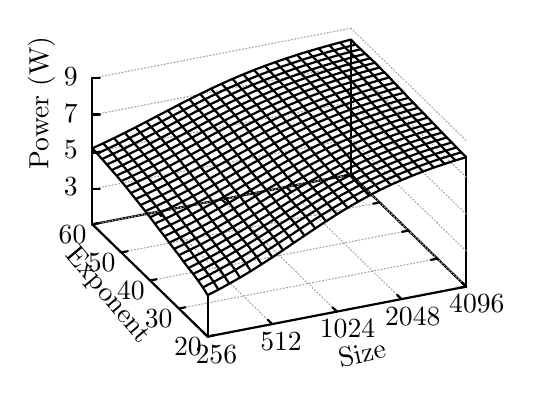
\begin{tikzpicture}[y=0.80pt, x=0.80pt, yscale=-0.570000, xscale=0.570000, inner sep=0pt, outer sep=0pt]
\begin{scope}[draw=black,line join=bevel,line cap=rect,even odd rule,line width=0.800pt]
  \begin{scope}[cm={{1.0,0.0,0.0,1.0,(0.0,0.0)}},draw=black,line join=bevel,line cap=rect,line width=0.800pt]
  \end{scope}
  \begin{scope}[cm={{1.00465,0.0,0.0,1.00465,(0.0,0.0)}},draw=black,line join=bevel,line cap=rect,line width=0.800pt]
  \end{scope}
  \begin{scope}[cm={{1.00465,0.0,0.0,1.00465,(0.0,0.0)}},draw=black,line join=round,line cap=round,line width=0.800pt]
    \path[draw] (67.6000,186.1000) -- (271.5000,146.8000);
    \path[draw] (362.4000,235.2000) -- (271.5000,146.8000);
    \path[draw] (67.5000,186.5000) -- (67.5000,70.5000);
    \path[draw] (271.5000,146.5000) -- (271.5000,40.5000);
    \path[draw] (362.5000,235.5000) -- (362.5000,133.5000);
  \end{scope}
  \begin{scope}[cm={{1.00465,0.0,0.0,1.00465,(0.0,0.0)}},draw=ca0a0a4,dash pattern=on 0.40pt off 0.80pt,line join=round,line cap=round,line width=0.400pt]
    \path[draw] (158.5000,274.6000) -- (67.6000,186.1000);
  \end{scope}
  \begin{scope}[cm={{1.00465,0.0,0.0,1.00465,(0.0,0.0)}},draw=black,line join=round,line cap=round,line width=0.800pt]
    \path[draw] (158.5000,274.6000) -- (155.1000,271.3000);
    \path[draw] (67.6000,186.1000) -- (71.0000,189.4000);
  \end{scope}
  \begin{scope}[cm={{1.00465,0.0,0.0,1.00465,(0.0,0.0)}},draw=black,line join=bevel,line cap=rect,line width=0.800pt]
  \end{scope}
  \begin{scope}[cm={{1.00465,0.0,0.0,1.00465,(149.693,296.874)}},draw=black,line join=bevel,line cap=rect,line width=0.800pt]
  \end{scope}
  \begin{scope}[cm={{1.00465,0.0,0.0,1.00465,(149.693,296.874)}},draw=black,line join=bevel,line cap=rect,line width=0.800pt]
  \end{scope}
  \begin{scope}[cm={{1.00465,0.0,0.0,1.00465,(149.693,296.874)}},draw=black,line join=bevel,line cap=rect,line width=0.800pt]
  \end{scope}
  \begin{scope}[cm={{1.00465,0.0,0.0,1.00465,(149.693,296.874)}},draw=black,line join=bevel,line cap=rect,line width=0.800pt]
  \end{scope}
  \begin{scope}[cm={{1.00465,0.0,0.0,1.00465,(149.693,296.874)}},draw=black,line join=bevel,line cap=rect,line width=0.800pt]
  \end{scope}
  \begin{scope}[cm={{1.00465,0.0,0.0,1.00465,(149.693,296.874)}},draw=black,line join=bevel,line cap=rect,line width=0.800pt]
    \path[fill=black] (0.0000,0.0000) node[above right] () {256};
  \end{scope}
  \begin{scope}[cm={{1.00465,0.0,0.0,1.00465,(149.693,296.874)}},draw=black,line join=bevel,line cap=rect,line width=0.800pt]
  \end{scope}
  \begin{scope}[cm={{1.00465,0.0,0.0,1.00465,(0.0,0.0)}},draw=black,line join=bevel,line cap=rect,line width=0.800pt]
  \end{scope}
  \begin{scope}[cm={{1.00465,0.0,0.0,1.00465,(0.0,0.0)}},draw=ca0a0a4,dash pattern=on 0.40pt off 0.80pt,line join=round,line cap=round,line width=0.400pt]
    \path[draw] (209.5000,264.8000) -- (118.6000,176.3000);
  \end{scope}
  \begin{scope}[cm={{1.00465,0.0,0.0,1.00465,(0.0,0.0)}},draw=black,line join=round,line cap=round,line width=0.800pt]
    \path[draw] (209.5000,264.8000) -- (206.1000,261.5000);
    \path[draw] (118.6000,176.3000) -- (122.0000,179.6000);
  \end{scope}
  \begin{scope}[cm={{1.00465,0.0,0.0,1.00465,(0.0,0.0)}},draw=black,line join=bevel,line cap=rect,line width=0.800pt]
  \end{scope}
  \begin{scope}[cm={{1.00465,0.0,0.0,1.00465,(200.93,286.828)}},draw=black,line join=bevel,line cap=rect,line width=0.800pt]
  \end{scope}
  \begin{scope}[cm={{1.00465,0.0,0.0,1.00465,(200.93,286.828)}},draw=black,line join=bevel,line cap=rect,line width=0.800pt]
  \end{scope}
  \begin{scope}[cm={{1.00465,0.0,0.0,1.00465,(200.93,286.828)}},draw=black,line join=bevel,line cap=rect,line width=0.800pt]
  \end{scope}
  \begin{scope}[cm={{1.00465,0.0,0.0,1.00465,(200.93,286.828)}},draw=black,line join=bevel,line cap=rect,line width=0.800pt]
  \end{scope}
  \begin{scope}[cm={{1.00465,0.0,0.0,1.00465,(200.93,286.828)}},draw=black,line join=bevel,line cap=rect,line width=0.800pt]
  \end{scope}
  \begin{scope}[cm={{1.00465,0.0,0.0,1.00465,(200.93,286.828)}},draw=black,line join=bevel,line cap=rect,line width=0.800pt]
    \path[fill=black] (0.0000,0.0000) node[above right] () {512};
  \end{scope}
  \begin{scope}[cm={{1.00465,0.0,0.0,1.00465,(200.93,286.828)}},draw=black,line join=bevel,line cap=rect,line width=0.800pt]
  \end{scope}
  \begin{scope}[cm={{1.00465,0.0,0.0,1.00465,(0.0,0.0)}},draw=black,line join=bevel,line cap=rect,line width=0.800pt]
  \end{scope}
  \begin{scope}[cm={{1.00465,0.0,0.0,1.00465,(0.0,0.0)}},draw=ca0a0a4,dash pattern=on 0.40pt off 0.80pt,line join=round,line cap=round,line width=0.400pt]
    \path[draw] (260.4000,254.9000) -- (169.6000,166.4000);
  \end{scope}
  \begin{scope}[cm={{1.00465,0.0,0.0,1.00465,(0.0,0.0)}},draw=black,line join=round,line cap=round,line width=0.800pt]
    \path[draw] (260.4000,254.9000) -- (257.0000,251.6000);
    \path[draw] (169.6000,166.4000) -- (173.0000,169.7000);
  \end{scope}
  \begin{scope}[cm={{1.00465,0.0,0.0,1.00465,(0.0,0.0)}},draw=black,line join=bevel,line cap=rect,line width=0.800pt]
  \end{scope}
  \begin{scope}[cm={{1.00465,0.0,0.0,1.00465,(248.149,276.781)}},draw=black,line join=bevel,line cap=rect,line width=0.800pt]
  \end{scope}
  \begin{scope}[cm={{1.00465,0.0,0.0,1.00465,(248.149,276.781)}},draw=black,line join=bevel,line cap=rect,line width=0.800pt]
  \end{scope}
  \begin{scope}[cm={{1.00465,0.0,0.0,1.00465,(248.149,276.781)}},draw=black,line join=bevel,line cap=rect,line width=0.800pt]
  \end{scope}
  \begin{scope}[cm={{1.00465,0.0,0.0,1.00465,(248.149,276.781)}},draw=black,line join=bevel,line cap=rect,line width=0.800pt]
  \end{scope}
  \begin{scope}[cm={{1.00465,0.0,0.0,1.00465,(248.149,276.781)}},draw=black,line join=bevel,line cap=rect,line width=0.800pt]
  \end{scope}
  \begin{scope}[cm={{1.00465,0.0,0.0,1.00465,(248.149,276.781)}},draw=black,line join=bevel,line cap=rect,line width=0.800pt]
    \path[fill=black] (0.0000,0.0000) node[above right] () {1024};
  \end{scope}
  \begin{scope}[cm={{1.00465,0.0,0.0,1.00465,(248.149,276.781)}},draw=black,line join=bevel,line cap=rect,line width=0.800pt]
  \end{scope}
  \begin{scope}[cm={{1.00465,0.0,0.0,1.00465,(0.0,0.0)}},draw=black,line join=bevel,line cap=rect,line width=0.800pt]
  \end{scope}
  \begin{scope}[cm={{1.00465,0.0,0.0,1.00465,(0.0,0.0)}},draw=ca0a0a4,dash pattern=on 0.40pt off 0.80pt,line join=round,line cap=round,line width=0.400pt]
    \path[draw] (311.4000,245.1000) -- (220.5000,156.6000);
  \end{scope}
  \begin{scope}[cm={{1.00465,0.0,0.0,1.00465,(0.0,0.0)}},draw=black,line join=round,line cap=round,line width=0.800pt]
    \path[draw] (311.4000,245.1000) -- (308.0000,241.8000);
    \path[draw] (220.5000,156.6000) -- (223.9000,159.9000);
  \end{scope}
  \begin{scope}[cm={{1.00465,0.0,0.0,1.00465,(0.0,0.0)}},draw=black,line join=bevel,line cap=rect,line width=0.800pt]
  \end{scope}
  \begin{scope}[cm={{1.00465,0.0,0.0,1.00465,(299.888,266.735)}},draw=black,line join=bevel,line cap=rect,line width=0.800pt]
  \end{scope}
  \begin{scope}[cm={{1.00465,0.0,0.0,1.00465,(299.888,266.735)}},draw=black,line join=bevel,line cap=rect,line width=0.800pt]
  \end{scope}
  \begin{scope}[cm={{1.00465,0.0,0.0,1.00465,(299.888,266.735)}},draw=black,line join=bevel,line cap=rect,line width=0.800pt]
  \end{scope}
  \begin{scope}[cm={{1.00465,0.0,0.0,1.00465,(299.888,266.735)}},draw=black,line join=bevel,line cap=rect,line width=0.800pt]
  \end{scope}
  \begin{scope}[cm={{1.00465,0.0,0.0,1.00465,(299.888,266.735)}},draw=black,line join=bevel,line cap=rect,line width=0.800pt]
  \end{scope}
  \begin{scope}[cm={{1.00465,0.0,0.0,1.00465,(299.888,266.735)}},draw=black,line join=bevel,line cap=rect,line width=0.800pt]
    \path[fill=black] (0.0000,0.0000) node[above right] () {2048};
  \end{scope}
  \begin{scope}[cm={{1.00465,0.0,0.0,1.00465,(299.888,266.735)}},draw=black,line join=bevel,line cap=rect,line width=0.800pt]
  \end{scope}
  \begin{scope}[cm={{1.00465,0.0,0.0,1.00465,(0.0,0.0)}},draw=black,line join=bevel,line cap=rect,line width=0.800pt]
  \end{scope}
  \begin{scope}[cm={{1.00465,0.0,0.0,1.00465,(0.0,0.0)}},draw=ca0a0a4,dash pattern=on 0.40pt off 0.80pt,line join=round,line cap=round,line width=0.400pt]
    \path[draw] (362.4000,235.2000) -- (271.5000,146.8000);
  \end{scope}
  \begin{scope}[cm={{1.00465,0.0,0.0,1.00465,(0.0,0.0)}},draw=black,line join=round,line cap=round,line width=0.800pt]
    \path[draw] (362.4000,235.2000) -- (359.0000,231.9000);
    \path[draw] (271.5000,146.8000) -- (274.9000,150.1000);
  \end{scope}
  \begin{scope}[cm={{1.00465,0.0,0.0,1.00465,(0.0,0.0)}},draw=black,line join=bevel,line cap=rect,line width=0.800pt]
  \end{scope}
  \begin{scope}[cm={{1.00465,0.0,0.0,1.00465,(350.623,256.688)}},draw=black,line join=bevel,line cap=rect,line width=0.800pt]
  \end{scope}
  \begin{scope}[cm={{1.00465,0.0,0.0,1.00465,(350.623,256.688)}},draw=black,line join=bevel,line cap=rect,line width=0.800pt]
  \end{scope}
  \begin{scope}[cm={{1.00465,0.0,0.0,1.00465,(350.623,256.688)}},draw=black,line join=bevel,line cap=rect,line width=0.800pt]
  \end{scope}
  \begin{scope}[cm={{1.00465,0.0,0.0,1.00465,(350.623,256.688)}},draw=black,line join=bevel,line cap=rect,line width=0.800pt]
  \end{scope}
  \begin{scope}[cm={{1.00465,0.0,0.0,1.00465,(350.623,256.688)}},draw=black,line join=bevel,line cap=rect,line width=0.800pt]
  \end{scope}
  \begin{scope}[cm={{1.00465,0.0,0.0,1.00465,(350.623,256.688)}},draw=black,line join=bevel,line cap=rect,line width=0.800pt]
    \path[fill=black] (0.0000,0.0000) node[above right] () {4096};
  \end{scope}
  \begin{scope}[cm={{1.00465,0.0,0.0,1.00465,(350.623,256.688)}},draw=black,line join=bevel,line cap=rect,line width=0.800pt]
  \end{scope}
  \begin{scope}[cm={{1.00465,0.0,0.0,1.00465,(0.0,0.0)}},draw=black,line join=bevel,line cap=rect,line width=0.800pt]
  \end{scope}
  \begin{scope}[cm={{1.00465,0.0,0.0,1.00465,(0.0,0.0)}},draw=ca0a0a4,dash pattern=on 0.40pt off 0.80pt,line join=round,line cap=round,line width=0.400pt]
    \path[draw] (158.5000,274.6000) -- (362.4000,235.2000);
  \end{scope}
  \begin{scope}[cm={{1.00465,0.0,0.0,1.00465,(0.0,0.0)}},draw=black,line join=round,line cap=round,line width=0.800pt]
    \path[draw] (158.5000,274.6000) -- (163.6000,273.6000);
    \path[draw] (362.4000,235.2000) -- (357.2000,236.2000);
  \end{scope}
  \begin{scope}[cm={{1.00465,0.0,0.0,1.00465,(0.0,0.0)}},draw=black,line join=bevel,line cap=rect,line width=0.800pt]
  \end{scope}
  \begin{scope}[cm={{1.00465,0.0,0.0,1.00465,(132.614,290.847)}},draw=black,line join=bevel,line cap=rect,line width=0.800pt]
  \end{scope}
  \begin{scope}[cm={{1.00465,0.0,0.0,1.00465,(132.614,290.847)}},draw=black,line join=bevel,line cap=rect,line width=0.800pt]
  \end{scope}
  \begin{scope}[cm={{1.00465,0.0,0.0,1.00465,(132.614,290.847)}},draw=black,line join=bevel,line cap=rect,line width=0.800pt]
  \end{scope}
  \begin{scope}[cm={{1.00465,0.0,0.0,1.00465,(132.614,290.847)}},draw=black,line join=bevel,line cap=rect,line width=0.800pt]
  \end{scope}
  \begin{scope}[cm={{1.00465,0.0,0.0,1.00465,(132.614,290.847)}},draw=black,line join=bevel,line cap=rect,line width=0.800pt]
  \end{scope}
  \begin{scope}[cm={{1.00465,0.0,0.0,1.00465,(132.614,290.847)}},draw=black,line join=bevel,line cap=rect,line width=0.800pt]
    \path[fill=black] (0.0000,0.0000) node[above right] () {20};
  \end{scope}
  \begin{scope}[cm={{1.00465,0.0,0.0,1.00465,(132.614,290.847)}},draw=black,line join=bevel,line cap=rect,line width=0.800pt]
  \end{scope}
  \begin{scope}[cm={{1.00465,0.0,0.0,1.00465,(0.0,0.0)}},draw=black,line join=bevel,line cap=rect,line width=0.800pt]
  \end{scope}
  \begin{scope}[cm={{1.00465,0.0,0.0,1.00465,(0.0,0.0)}},draw=ca0a0a4,dash pattern=on 0.40pt off 0.80pt,line join=round,line cap=round,line width=0.400pt]
    \path[draw] (135.8000,252.5000) -- (339.7000,213.1000);
  \end{scope}
  \begin{scope}[cm={{1.00465,0.0,0.0,1.00465,(0.0,0.0)}},draw=black,line join=round,line cap=round,line width=0.800pt]
    \path[draw] (135.8000,252.5000) -- (140.9000,251.5000);
    \path[draw] (339.7000,213.1000) -- (334.5000,214.1000);
  \end{scope}
  \begin{scope}[cm={{1.00465,0.0,0.0,1.00465,(0.0,0.0)}},draw=black,line join=bevel,line cap=rect,line width=0.800pt]
  \end{scope}
  \begin{scope}[cm={{1.00465,0.0,0.0,1.00465,(109.507,268.744)}},draw=black,line join=bevel,line cap=rect,line width=0.800pt]
  \end{scope}
  \begin{scope}[cm={{1.00465,0.0,0.0,1.00465,(109.507,268.744)}},draw=black,line join=bevel,line cap=rect,line width=0.800pt]
  \end{scope}
  \begin{scope}[cm={{1.00465,0.0,0.0,1.00465,(109.507,268.744)}},draw=black,line join=bevel,line cap=rect,line width=0.800pt]
  \end{scope}
  \begin{scope}[cm={{1.00465,0.0,0.0,1.00465,(109.507,268.744)}},draw=black,line join=bevel,line cap=rect,line width=0.800pt]
  \end{scope}
  \begin{scope}[cm={{1.00465,0.0,0.0,1.00465,(109.507,268.744)}},draw=black,line join=bevel,line cap=rect,line width=0.800pt]
  \end{scope}
  \begin{scope}[cm={{1.00465,0.0,0.0,1.00465,(109.507,268.744)}},draw=black,line join=bevel,line cap=rect,line width=0.800pt]
    \path[fill=black] (0.0000,0.0000) node[above right] () {30};
  \end{scope}
  \begin{scope}[cm={{1.00465,0.0,0.0,1.00465,(109.507,268.744)}},draw=black,line join=bevel,line cap=rect,line width=0.800pt]
  \end{scope}
  \begin{scope}[cm={{1.00465,0.0,0.0,1.00465,(0.0,0.0)}},draw=black,line join=bevel,line cap=rect,line width=0.800pt]
  \end{scope}
  \begin{scope}[cm={{1.00465,0.0,0.0,1.00465,(0.0,0.0)}},draw=ca0a0a4,dash pattern=on 0.40pt off 0.80pt,line join=round,line cap=round,line width=0.400pt]
    \path[draw] (113.1000,230.4000) -- (316.9000,191.0000);
  \end{scope}
  \begin{scope}[cm={{1.00465,0.0,0.0,1.00465,(0.0,0.0)}},draw=black,line join=round,line cap=round,line width=0.800pt]
    \path[draw] (113.1000,230.4000) -- (118.2000,229.4000);
    \path[draw] (316.9000,191.0000) -- (311.8000,192.0000);
  \end{scope}
  \begin{scope}[cm={{1.00465,0.0,0.0,1.00465,(0.0,0.0)}},draw=black,line join=bevel,line cap=rect,line width=0.800pt]
  \end{scope}
  \begin{scope}[cm={{1.00465,0.0,0.0,1.00465,(87.4047,246.642)}},draw=black,line join=bevel,line cap=rect,line width=0.800pt]
  \end{scope}
  \begin{scope}[cm={{1.00465,0.0,0.0,1.00465,(87.4047,246.642)}},draw=black,line join=bevel,line cap=rect,line width=0.800pt]
  \end{scope}
  \begin{scope}[cm={{1.00465,0.0,0.0,1.00465,(87.4047,246.642)}},draw=black,line join=bevel,line cap=rect,line width=0.800pt]
  \end{scope}
  \begin{scope}[cm={{1.00465,0.0,0.0,1.00465,(87.4047,246.642)}},draw=black,line join=bevel,line cap=rect,line width=0.800pt]
  \end{scope}
  \begin{scope}[cm={{1.00465,0.0,0.0,1.00465,(87.4047,246.642)}},draw=black,line join=bevel,line cap=rect,line width=0.800pt]
  \end{scope}
  \begin{scope}[cm={{1.00465,0.0,0.0,1.00465,(87.4047,246.642)}},draw=black,line join=bevel,line cap=rect,line width=0.800pt]
    \path[fill=black] (0.0000,0.0000) node[above right] () {40};
  \end{scope}
  \begin{scope}[cm={{1.00465,0.0,0.0,1.00465,(87.4047,246.642)}},draw=black,line join=bevel,line cap=rect,line width=0.800pt]
  \end{scope}
  \begin{scope}[cm={{1.00465,0.0,0.0,1.00465,(0.0,0.0)}},draw=black,line join=bevel,line cap=rect,line width=0.800pt]
  \end{scope}
  \begin{scope}[cm={{1.00465,0.0,0.0,1.00465,(0.0,0.0)}},draw=ca0a0a4,dash pattern=on 0.40pt off 0.80pt,line join=round,line cap=round,line width=0.400pt]
    \path[draw] (90.3000,208.2000) -- (294.2000,168.8000);
  \end{scope}
  \begin{scope}[cm={{1.00465,0.0,0.0,1.00465,(0.0,0.0)}},draw=black,line join=round,line cap=round,line width=0.800pt]
    \path[draw] (90.3000,208.2000) -- (95.5000,207.3000);
    \path[draw] (294.2000,168.8000) -- (289.1000,169.8000);
  \end{scope}
  \begin{scope}[cm={{1.00465,0.0,0.0,1.00465,(0.0,0.0)}},draw=black,line join=bevel,line cap=rect,line width=0.800pt]
  \end{scope}
  \begin{scope}[cm={{1.00465,0.0,0.0,1.00465,(64.2977,224.54)}},draw=black,line join=bevel,line cap=rect,line width=0.800pt]
  \end{scope}
  \begin{scope}[cm={{1.00465,0.0,0.0,1.00465,(64.2977,224.54)}},draw=black,line join=bevel,line cap=rect,line width=0.800pt]
  \end{scope}
  \begin{scope}[cm={{1.00465,0.0,0.0,1.00465,(64.2977,224.54)}},draw=black,line join=bevel,line cap=rect,line width=0.800pt]
  \end{scope}
  \begin{scope}[cm={{1.00465,0.0,0.0,1.00465,(64.2977,224.54)}},draw=black,line join=bevel,line cap=rect,line width=0.800pt]
  \end{scope}
  \begin{scope}[cm={{1.00465,0.0,0.0,1.00465,(64.2977,224.54)}},draw=black,line join=bevel,line cap=rect,line width=0.800pt]
  \end{scope}
  \begin{scope}[cm={{1.00465,0.0,0.0,1.00465,(64.2977,224.54)}},draw=black,line join=bevel,line cap=rect,line width=0.800pt]
    \path[fill=black] (0.0000,0.0000) node[above right] () {50};
  \end{scope}
  \begin{scope}[cm={{1.00465,0.0,0.0,1.00465,(64.2977,224.54)}},draw=black,line join=bevel,line cap=rect,line width=0.800pt]
  \end{scope}
  \begin{scope}[cm={{1.00465,0.0,0.0,1.00465,(0.0,0.0)}},draw=black,line join=bevel,line cap=rect,line width=0.800pt]
  \end{scope}
  \begin{scope}[cm={{1.00465,0.0,0.0,1.00465,(0.0,0.0)}},draw=ca0a0a4,dash pattern=on 0.40pt off 0.80pt,line join=round,line cap=round,line width=0.400pt]
    \path[draw] (67.6000,186.1000) -- (271.5000,146.8000);
  \end{scope}
  \begin{scope}[cm={{1.00465,0.0,0.0,1.00465,(0.0,0.0)}},draw=black,line join=round,line cap=round,line width=0.800pt]
    \path[draw] (67.6000,186.1000) -- (72.8000,185.1000);
    \path[draw] (271.5000,146.8000) -- (266.4000,147.8000);
  \end{scope}
  \begin{scope}[cm={{1.00465,0.0,0.0,1.00465,(0.0,0.0)}},draw=black,line join=bevel,line cap=rect,line width=0.800pt]
  \end{scope}
  \begin{scope}[cm={{1.00465,0.0,0.0,1.00465,(41.1907,202.437)}},draw=black,line join=bevel,line cap=rect,line width=0.800pt]
  \end{scope}
  \begin{scope}[cm={{1.00465,0.0,0.0,1.00465,(41.1907,202.437)}},draw=black,line join=bevel,line cap=rect,line width=0.800pt]
  \end{scope}
  \begin{scope}[cm={{1.00465,0.0,0.0,1.00465,(41.1907,202.437)}},draw=black,line join=bevel,line cap=rect,line width=0.800pt]
  \end{scope}
  \begin{scope}[cm={{1.00465,0.0,0.0,1.00465,(41.1907,202.437)}},draw=black,line join=bevel,line cap=rect,line width=0.800pt]
  \end{scope}
  \begin{scope}[cm={{1.00465,0.0,0.0,1.00465,(41.1907,202.437)}},draw=black,line join=bevel,line cap=rect,line width=0.800pt]
  \end{scope}
  \begin{scope}[cm={{1.00465,0.0,0.0,1.00465,(41.1907,202.437)}},draw=black,line join=bevel,line cap=rect,line width=0.800pt]
    \path[fill=black] (0.0000,0.0000) node[above right] () {60};
  \end{scope}
  \begin{scope}[cm={{1.00465,0.0,0.0,1.00465,(41.1907,202.437)}},draw=black,line join=bevel,line cap=rect,line width=0.800pt]
  \end{scope}
  \begin{scope}[cm={{1.00465,0.0,0.0,1.00465,(0.0,0.0)}},draw=black,line join=bevel,line cap=rect,line width=0.800pt]
  \end{scope}
  \begin{scope}[cm={{1.00465,0.0,0.0,1.00465,(0.0,0.0)}},draw=ca0a0a4,dash pattern=on 0.40pt off 0.80pt,line join=round,line cap=round,line width=0.400pt]
    \path[draw] (67.6000,158.1000) -- (271.5000,118.8000);
    \path[draw] (271.5000,118.8000) -- (271.5000,118.8000) -- (362.4000,207.2000);
  \end{scope}
  \begin{scope}[cm={{1.00465,0.0,0.0,1.00465,(0.0,0.0)}},draw=black,line join=round,line cap=round,line width=0.800pt]
    \path[draw] (67.5000,158.5000) -- (73.5000,158.5000);
  \end{scope}
  \begin{scope}[cm={{1.00465,0.0,0.0,1.00465,(0.0,0.0)}},draw=black,line join=bevel,line cap=rect,line width=0.800pt]
  \end{scope}
  \begin{scope}[cm={{1.00465,0.0,0.0,1.00465,(45.2093,164.26)}},draw=black,line join=bevel,line cap=rect,line width=0.800pt]
  \end{scope}
  \begin{scope}[cm={{1.00465,0.0,0.0,1.00465,(45.2093,164.26)}},draw=black,line join=bevel,line cap=rect,line width=0.800pt]
  \end{scope}
  \begin{scope}[cm={{1.00465,0.0,0.0,1.00465,(45.2093,164.26)}},draw=black,line join=bevel,line cap=rect,line width=0.800pt]
  \end{scope}
  \begin{scope}[cm={{1.00465,0.0,0.0,1.00465,(45.2093,164.26)}},draw=black,line join=bevel,line cap=rect,line width=0.800pt]
  \end{scope}
  \begin{scope}[cm={{1.00465,0.0,0.0,1.00465,(45.2093,164.26)}},draw=black,line join=bevel,line cap=rect,line width=0.800pt]
  \end{scope}
  \begin{scope}[cm={{1.00465,0.0,0.0,1.00465,(45.2093,164.26)}},draw=black,line join=bevel,line cap=rect,line width=0.800pt]
    \path[fill=black] (0.0000,0.0000) node[above right] () {3};
  \end{scope}
  \begin{scope}[cm={{1.00465,0.0,0.0,1.00465,(45.2093,164.26)}},draw=black,line join=bevel,line cap=rect,line width=0.800pt]
  \end{scope}
  \begin{scope}[cm={{1.00465,0.0,0.0,1.00465,(0.0,0.0)}},draw=black,line join=bevel,line cap=rect,line width=0.800pt]
  \end{scope}
  \begin{scope}[cm={{1.00465,0.0,0.0,1.00465,(0.0,0.0)}},draw=ca0a0a4,dash pattern=on 0.40pt off 0.80pt,line join=round,line cap=round,line width=0.400pt]
    \path[draw] (67.6000,129.1000) -- (271.5000,89.7000);
    \path[draw] (271.5000,89.7000) -- (271.5000,89.7000) -- (362.4000,178.1000);
  \end{scope}
  \begin{scope}[cm={{1.00465,0.0,0.0,1.00465,(0.0,0.0)}},draw=black,line join=round,line cap=round,line width=0.800pt]
    \path[draw] (67.5000,129.5000) -- (73.5000,129.5000);
  \end{scope}
  \begin{scope}[cm={{1.00465,0.0,0.0,1.00465,(0.0,0.0)}},draw=black,line join=bevel,line cap=rect,line width=0.800pt]
  \end{scope}
  \begin{scope}[cm={{1.00465,0.0,0.0,1.00465,(45.2093,135.126)}},draw=black,line join=bevel,line cap=rect,line width=0.800pt]
  \end{scope}
  \begin{scope}[cm={{1.00465,0.0,0.0,1.00465,(45.2093,135.126)}},draw=black,line join=bevel,line cap=rect,line width=0.800pt]
  \end{scope}
  \begin{scope}[cm={{1.00465,0.0,0.0,1.00465,(45.2093,135.126)}},draw=black,line join=bevel,line cap=rect,line width=0.800pt]
  \end{scope}
  \begin{scope}[cm={{1.00465,0.0,0.0,1.00465,(45.2093,135.126)}},draw=black,line join=bevel,line cap=rect,line width=0.800pt]
  \end{scope}
  \begin{scope}[cm={{1.00465,0.0,0.0,1.00465,(45.2093,135.126)}},draw=black,line join=bevel,line cap=rect,line width=0.800pt]
  \end{scope}
  \begin{scope}[cm={{1.00465,0.0,0.0,1.00465,(45.2093,135.126)}},draw=black,line join=bevel,line cap=rect,line width=0.800pt]
    \path[fill=black] (0.0000,0.0000) node[above right] () {5};
  \end{scope}
  \begin{scope}[cm={{1.00465,0.0,0.0,1.00465,(45.2093,135.126)}},draw=black,line join=bevel,line cap=rect,line width=0.800pt]
  \end{scope}
  \begin{scope}[cm={{1.00465,0.0,0.0,1.00465,(0.0,0.0)}},draw=black,line join=bevel,line cap=rect,line width=0.800pt]
  \end{scope}
  \begin{scope}[cm={{1.00465,0.0,0.0,1.00465,(0.0,0.0)}},draw=ca0a0a4,dash pattern=on 0.40pt off 0.80pt,line join=round,line cap=round,line width=0.400pt]
    \path[draw] (67.6000,99.9000) -- (271.5000,60.5000);
    \path[draw] (271.5000,60.5000) -- (271.5000,60.5000) -- (362.4000,149.0000);
  \end{scope}
  \begin{scope}[cm={{1.00465,0.0,0.0,1.00465,(0.0,0.0)}},draw=black,line join=round,line cap=round,line width=0.800pt]
    \path[draw] (67.5000,99.5000) -- (73.5000,99.5000);
  \end{scope}
  \begin{scope}[cm={{1.00465,0.0,0.0,1.00465,(0.0,0.0)}},draw=black,line join=bevel,line cap=rect,line width=0.800pt]
  \end{scope}
  \begin{scope}[cm={{1.00465,0.0,0.0,1.00465,(45.2093,105.991)}},draw=black,line join=bevel,line cap=rect,line width=0.800pt]
  \end{scope}
  \begin{scope}[cm={{1.00465,0.0,0.0,1.00465,(45.2093,105.991)}},draw=black,line join=bevel,line cap=rect,line width=0.800pt]
  \end{scope}
  \begin{scope}[cm={{1.00465,0.0,0.0,1.00465,(45.2093,105.991)}},draw=black,line join=bevel,line cap=rect,line width=0.800pt]
  \end{scope}
  \begin{scope}[cm={{1.00465,0.0,0.0,1.00465,(45.2093,105.991)}},draw=black,line join=bevel,line cap=rect,line width=0.800pt]
  \end{scope}
  \begin{scope}[cm={{1.00465,0.0,0.0,1.00465,(45.2093,105.991)}},draw=black,line join=bevel,line cap=rect,line width=0.800pt]
  \end{scope}
  \begin{scope}[cm={{1.00465,0.0,0.0,1.00465,(45.2093,105.991)}},draw=black,line join=bevel,line cap=rect,line width=0.800pt]
    \path[fill=black] (0.0000,0.0000) node[above right] () {7};
  \end{scope}
  \begin{scope}[cm={{1.00465,0.0,0.0,1.00465,(45.2093,105.991)}},draw=black,line join=bevel,line cap=rect,line width=0.800pt]
  \end{scope}
  \begin{scope}[cm={{1.00465,0.0,0.0,1.00465,(0.0,0.0)}},draw=black,line join=bevel,line cap=rect,line width=0.800pt]
  \end{scope}
  \begin{scope}[cm={{1.00465,0.0,0.0,1.00465,(0.0,0.0)}},draw=ca0a0a4,dash pattern=on 0.40pt off 0.80pt,line join=round,line cap=round,line width=0.400pt]
    \path[draw] (67.6000,70.8000) -- (271.5000,31.4000);
    \path[draw] (271.5000,31.4000) -- (271.5000,31.4000) -- (362.4000,119.9000);
  \end{scope}
  \begin{scope}[cm={{1.00465,0.0,0.0,1.00465,(0.0,0.0)}},draw=black,line join=round,line cap=round,line width=0.800pt]
    \path[draw] (67.5000,70.5000) -- (73.5000,70.5000);
  \end{scope}
  \begin{scope}[cm={{1.00465,0.0,0.0,1.00465,(0.0,0.0)}},draw=black,line join=bevel,line cap=rect,line width=0.800pt]
  \end{scope}
  \begin{scope}[cm={{1.00465,0.0,0.0,1.00465,(45.2093,76.8558)}},draw=black,line join=bevel,line cap=rect,line width=0.800pt]
  \end{scope}
  \begin{scope}[cm={{1.00465,0.0,0.0,1.00465,(45.2093,76.8558)}},draw=black,line join=bevel,line cap=rect,line width=0.800pt]
  \end{scope}
  \begin{scope}[cm={{1.00465,0.0,0.0,1.00465,(45.2093,76.8558)}},draw=black,line join=bevel,line cap=rect,line width=0.800pt]
  \end{scope}
  \begin{scope}[cm={{1.00465,0.0,0.0,1.00465,(45.2093,76.8558)}},draw=black,line join=bevel,line cap=rect,line width=0.800pt]
  \end{scope}
  \begin{scope}[cm={{1.00465,0.0,0.0,1.00465,(45.2093,76.8558)}},draw=black,line join=bevel,line cap=rect,line width=0.800pt]
  \end{scope}
  \begin{scope}[cm={{1.00465,0.0,0.0,1.00465,(45.2093,76.8558)}},draw=black,line join=bevel,line cap=rect,line width=0.800pt]
    \path[fill=black] (0.0000,0.0000) node[above right] () {9};
  \end{scope}
  \begin{scope}[cm={{1.00465,0.0,0.0,1.00465,(45.2093,76.8558)}},draw=black,line join=bevel,line cap=rect,line width=0.800pt]
  \end{scope}
  \begin{scope}[cm={{0.0,-1.00465,1.00465,0.0,(24.614,149.191)}},draw=black,line join=bevel,line cap=rect,line width=0.800pt]
  \end{scope}
  \begin{scope}[cm={{0.0,-1.00465,1.00465,0.0,(24.614,149.191)}},draw=black,line join=bevel,line cap=rect,line width=0.800pt]
  \end{scope}
  \begin{scope}[cm={{0.0,-1.00465,1.00465,0.0,(24.614,149.191)}},draw=black,line join=bevel,line cap=rect,line width=0.800pt]
  \end{scope}
  \begin{scope}[cm={{0.0,-1.00465,1.00465,0.0,(24.614,149.191)}},draw=black,line join=bevel,line cap=rect,line width=0.800pt]
  \end{scope}
  \begin{scope}[cm={{0.0,-1.00465,1.00465,0.0,(24.614,149.191)}},draw=black,line join=bevel,line cap=rect,line width=0.800pt]
  \end{scope}
  \begin{scope}[cm={{0.0,-1.00465,1.00465,0.0,(16.614,143.163)}},draw=black,line join=bevel,line cap=rect,line width=0.800pt]
    \path[fill=black] (0.0000,0.0000) node[above right] () {\rotatebox{90}{Power (W)}};
  \end{scope}
  \begin{scope}[cm={{0.0,-1.00465,1.00465,0.0,(24.614,149.191)}},draw=black,line join=bevel,line cap=rect,line width=0.800pt]
  \end{scope}
  \begin{scope}[cm={{1.00465,0.0,0.0,1.00465,(0.0,0.0)}},draw=black,line join=bevel,line cap=rect,line width=0.800pt]
  \end{scope}
  \begin{scope}[cm={{1.00465,0.0,0.0,1.00465,(0.0,0.0)}},draw=black,line join=bevel,line cap=rect,line width=0.800pt]
  \end{scope}
  \begin{scope}[cm={{1.00465,0.0,0.0,1.00465,(0.0,0.0)}},draw=black,line join=bevel,line cap=rect,line width=0.800pt]
  \end{scope}
  \begin{scope}[cm={{1.00465,0.0,0.0,1.00465,(0.0,0.0)}},draw=black,line join=round,line cap=round,line width=0.800pt]
    \path[draw] (362.4000,133.1000) -- (358.6000,129.3000) -- (358.6000,129.3000) --
      (354.8000,125.4000) -- (354.8000,125.4000) -- (351.0000,121.5000) --
      (351.0000,121.5000) -- (347.2000,117.6000) -- (347.2000,117.6000) --
      (343.4000,113.7000) -- (343.4000,113.7000) -- (339.7000,109.8000) --
      (339.7000,109.8000) -- (335.9000,105.9000) -- (335.9000,105.9000) --
      (332.1000,101.9000) -- (332.1000,101.9000) -- (328.3000,98.0000) --
      (328.3000,98.0000) -- (324.5000,94.1000) -- (324.5000,94.1000) --
      (320.7000,90.2000) -- (320.7000,90.2000) -- (316.9000,86.3000) --
      (316.9000,86.3000) -- (313.2000,82.2000) -- (313.2000,82.2000) --
      (309.4000,78.2000) -- (309.4000,78.2000) -- (305.6000,74.3000) --
      (305.6000,74.3000) -- (301.8000,70.2000) -- (301.8000,70.2000) --
      (298.0000,66.2000) -- (298.0000,66.2000) -- (294.2000,62.4000) --
      (294.2000,62.4000) -- (290.5000,58.6000) -- (290.5000,58.6000) --
      (286.7000,55.1000) -- (286.7000,55.1000) -- (282.9000,51.5000) --
      (282.9000,51.5000) -- (279.1000,47.9000) -- (279.1000,47.9000) --
      (275.3000,44.3000) -- (275.3000,44.3000) -- (271.5000,40.4000);
    \path[draw] (353.9000,135.7000) -- (350.1000,131.8000) -- (350.1000,131.8000) --
      (346.3000,128.0000) -- (346.3000,128.0000) -- (342.5000,124.1000) --
      (342.5000,124.1000) -- (338.7000,120.1000) -- (338.7000,120.1000) --
      (334.9000,116.2000) -- (334.9000,116.2000) -- (331.2000,112.3000) --
      (331.2000,112.3000) -- (327.4000,108.4000) -- (327.4000,108.4000) --
      (323.6000,104.4000) -- (323.6000,104.4000) -- (319.8000,100.5000) --
      (319.8000,100.5000) -- (316.0000,96.6000) -- (316.0000,96.6000) --
      (312.2000,92.6000) -- (312.2000,92.6000) -- (308.4000,88.7000) --
      (308.4000,88.7000) -- (304.7000,84.7000) -- (304.7000,84.7000) --
      (300.9000,80.6000) -- (300.9000,80.6000) -- (297.1000,76.7000) --
      (297.1000,76.7000) -- (293.3000,72.6000) -- (293.3000,72.6000) --
      (289.5000,68.6000) -- (289.5000,68.6000) -- (285.7000,64.7000) --
      (285.7000,64.7000) -- (282.0000,60.9000) -- (282.0000,60.9000) --
      (278.2000,57.4000) -- (278.2000,57.4000) -- (274.4000,53.8000) --
      (274.4000,53.8000) -- (270.6000,50.2000) -- (270.6000,50.2000) --
      (266.8000,46.5000) -- (266.8000,46.5000) -- (263.0000,42.6000);
    \path[draw] (345.4000,138.4000) -- (341.6000,134.5000) -- (341.6000,134.5000) --
      (337.8000,130.7000) -- (337.8000,130.7000) -- (334.0000,126.8000) --
      (334.0000,126.8000) -- (330.2000,122.8000) -- (330.2000,122.8000) --
      (326.4000,118.9000) -- (326.4000,118.9000) -- (322.7000,115.0000) --
      (322.7000,115.0000) -- (318.9000,111.0000) -- (318.9000,111.0000) --
      (315.1000,107.1000) -- (315.1000,107.1000) -- (311.3000,103.2000) --
      (311.3000,103.2000) -- (307.5000,99.2000) -- (307.5000,99.2000) --
      (303.7000,95.2000) -- (303.7000,95.2000) -- (299.9000,91.3000) --
      (299.9000,91.3000) -- (296.2000,87.2000) -- (296.2000,87.2000) --
      (292.4000,83.2000) -- (292.4000,83.2000) -- (288.6000,79.2000) --
      (288.6000,79.2000) -- (284.8000,75.1000) -- (284.8000,75.1000) --
      (281.0000,71.0000) -- (281.0000,71.0000) -- (277.2000,67.1000) --
      (277.2000,67.1000) -- (273.5000,63.4000) -- (273.5000,63.4000) --
      (269.7000,59.7000) -- (269.7000,59.7000) -- (265.9000,56.2000) --
      (265.9000,56.2000) -- (262.1000,52.5000) -- (262.1000,52.5000) --
      (258.3000,48.8000) -- (258.3000,48.8000) -- (254.5000,44.9000);
    \path[draw] (336.9000,141.3000) -- (333.1000,137.4000) -- (333.1000,137.4000) --
      (329.3000,133.5000) -- (329.3000,133.5000) -- (325.5000,129.6000) --
      (325.5000,129.6000) -- (321.7000,125.7000) -- (321.7000,125.7000) --
      (317.9000,121.8000) -- (317.9000,121.8000) -- (314.2000,117.8000) --
      (314.2000,117.8000) -- (310.4000,113.9000) -- (310.4000,113.9000) --
      (306.6000,109.9000) -- (306.6000,109.9000) -- (302.8000,105.9000) --
      (302.8000,105.9000) -- (299.0000,101.9000) -- (299.0000,101.9000) --
      (295.2000,97.9000) -- (295.2000,97.9000) -- (291.4000,94.0000) --
      (291.4000,94.0000) -- (287.7000,89.9000) -- (287.7000,89.9000) --
      (283.9000,85.8000) -- (283.9000,85.8000) -- (280.1000,81.8000) --
      (280.1000,81.8000) -- (276.3000,77.7000) -- (276.3000,77.7000) --
      (272.5000,73.6000) -- (272.5000,73.6000) -- (268.7000,69.7000) --
      (268.7000,69.7000) -- (265.0000,65.9000) -- (265.0000,65.9000) --
      (261.2000,62.3000) -- (261.2000,62.3000) -- (257.4000,58.7000) --
      (257.4000,58.7000) -- (253.6000,55.0000) -- (253.6000,55.0000) --
      (249.8000,51.2000) -- (249.8000,51.2000) -- (246.0000,47.3000);
    \path[draw] (328.4000,144.4000) -- (324.6000,140.5000) -- (324.6000,140.5000) --
      (320.8000,136.6000) -- (320.8000,136.6000) -- (317.0000,132.7000) --
      (317.0000,132.7000) -- (313.2000,128.7000) -- (313.2000,128.7000) --
      (309.4000,124.8000) -- (309.4000,124.8000) -- (305.7000,120.9000) --
      (305.7000,120.9000) -- (301.9000,116.9000) -- (301.9000,116.9000) --
      (298.1000,112.9000) -- (298.1000,112.9000) -- (294.3000,108.9000) --
      (294.3000,108.9000) -- (290.5000,104.8000) -- (290.5000,104.8000) --
      (286.7000,100.8000) -- (286.7000,100.8000) -- (282.9000,96.8000) --
      (282.9000,96.8000) -- (279.2000,92.7000) -- (279.2000,92.7000) --
      (275.4000,88.6000) -- (275.4000,88.6000) -- (271.6000,84.6000) --
      (271.6000,84.6000) -- (267.8000,80.4000) -- (267.8000,80.4000) --
      (264.0000,76.3000) -- (264.0000,76.3000) -- (260.2000,72.4000) --
      (260.2000,72.4000) -- (256.5000,68.6000) -- (256.5000,68.6000) --
      (252.7000,64.9000) -- (252.7000,64.9000) -- (248.9000,61.3000) --
      (248.9000,61.3000) -- (245.1000,57.5000) -- (245.1000,57.5000) --
      (241.3000,53.8000) -- (241.3000,53.8000) -- (237.5000,49.8000);
    \path[draw] (319.9000,147.7000) -- (316.1000,143.8000) -- (316.1000,143.8000) --
      (312.3000,139.8000) -- (312.3000,139.8000) -- (308.5000,135.9000) --
      (308.5000,135.9000) -- (304.7000,132.0000) -- (304.7000,132.0000) --
      (300.9000,128.1000) -- (300.9000,128.1000) -- (297.2000,124.1000) --
      (297.2000,124.1000) -- (293.4000,120.1000) -- (293.4000,120.1000) --
      (289.6000,116.0000) -- (289.6000,116.0000) -- (285.8000,112.0000) --
      (285.8000,112.0000) -- (282.0000,107.9000) -- (282.0000,107.9000) --
      (278.2000,103.9000) -- (278.2000,103.9000) -- (274.4000,99.8000) --
      (274.4000,99.8000) -- (270.7000,95.7000) -- (270.7000,95.7000) --
      (266.9000,91.6000) -- (266.9000,91.6000) -- (263.1000,87.5000) --
      (263.1000,87.5000) -- (259.3000,83.3000) -- (259.3000,83.3000) --
      (255.5000,79.2000) -- (255.5000,79.2000) -- (251.7000,75.2000) --
      (251.7000,75.2000) -- (248.0000,71.4000) -- (248.0000,71.4000) --
      (244.2000,67.7000) -- (244.2000,67.7000) -- (240.4000,64.0000) --
      (240.4000,64.0000) -- (236.6000,60.2000) -- (236.6000,60.2000) --
      (232.8000,56.4000) -- (232.8000,56.4000) -- (229.0000,52.4000);
    \path[draw] (311.4000,151.2000) -- (307.6000,147.3000) -- (307.6000,147.3000) --
      (303.8000,143.3000) -- (303.8000,143.3000) -- (300.0000,139.4000) --
      (300.0000,139.4000) -- (296.2000,135.5000) -- (296.2000,135.5000) --
      (292.4000,131.5000) -- (292.4000,131.5000) -- (288.7000,127.6000) --
      (288.7000,127.6000) -- (284.9000,123.5000) -- (284.9000,123.5000) --
      (281.1000,119.4000) -- (281.1000,119.4000) -- (277.3000,115.3000) --
      (277.3000,115.3000) -- (273.5000,111.2000) -- (273.5000,111.2000) --
      (269.7000,107.1000) -- (269.7000,107.1000) -- (265.9000,103.1000) --
      (265.9000,103.1000) -- (262.2000,98.9000) -- (262.2000,98.9000) --
      (258.4000,94.7000) -- (258.4000,94.7000) -- (254.6000,90.6000) --
      (254.6000,90.6000) -- (250.8000,86.4000) -- (250.8000,86.4000) --
      (247.0000,82.3000) -- (247.0000,82.3000) -- (243.2000,78.3000) --
      (243.2000,78.3000) -- (239.5000,74.4000) -- (239.5000,74.4000) --
      (235.7000,70.6000) -- (235.7000,70.6000) -- (231.9000,66.9000) --
      (231.9000,66.9000) -- (228.1000,63.0000) -- (228.1000,63.0000) --
      (224.3000,59.2000) -- (224.3000,59.2000) -- (220.5000,55.2000);
    \path[draw] (302.9000,154.9000) -- (299.1000,151.0000) -- (299.1000,151.0000) --
      (295.3000,147.1000) -- (295.3000,147.1000) -- (291.5000,143.1000) --
      (291.5000,143.1000) -- (287.7000,139.2000) -- (287.7000,139.2000) --
      (283.9000,135.2000) -- (283.9000,135.2000) -- (280.2000,131.2000) --
      (280.2000,131.2000) -- (276.4000,127.1000) -- (276.4000,127.1000) --
      (272.6000,123.0000) -- (272.6000,123.0000) -- (268.8000,118.9000) --
      (268.8000,118.9000) -- (265.0000,114.7000) -- (265.0000,114.7000) --
      (261.2000,110.6000) -- (261.2000,110.6000) -- (257.4000,106.5000) --
      (257.4000,106.5000) -- (253.7000,102.3000) -- (253.7000,102.3000) --
      (249.9000,98.1000) -- (249.9000,98.1000) -- (246.1000,93.9000) --
      (246.1000,93.9000) -- (242.3000,89.7000) -- (242.3000,89.7000) --
      (238.5000,85.5000) -- (238.5000,85.5000) -- (234.7000,81.4000) --
      (234.7000,81.4000) -- (231.0000,77.5000) -- (231.0000,77.5000) --
      (227.2000,73.7000) -- (227.2000,73.7000) -- (223.4000,69.9000) --
      (223.4000,69.9000) -- (219.6000,66.0000) -- (219.6000,66.0000) --
      (215.8000,62.1000) -- (215.8000,62.1000) -- (212.1000,58.1000);
    \path[draw] (294.4000,159.0000) -- (290.6000,155.0000) -- (290.6000,155.0000) --
      (286.8000,151.1000) -- (286.8000,151.1000) -- (283.0000,147.1000) --
      (283.0000,147.1000) -- (279.2000,143.1000) -- (279.2000,143.1000) --
      (275.4000,139.2000) -- (275.4000,139.2000) -- (271.7000,135.2000) --
      (271.7000,135.2000) -- (267.9000,131.0000) -- (267.9000,131.0000) --
      (264.1000,126.8000) -- (264.1000,126.8000) -- (260.3000,122.6000) --
      (260.3000,122.6000) -- (256.5000,118.4000) -- (256.5000,118.4000) --
      (252.7000,114.3000) -- (252.7000,114.3000) -- (248.9000,110.1000) --
      (248.9000,110.1000) -- (245.2000,105.8000) -- (245.2000,105.8000) --
      (241.4000,101.6000) -- (241.4000,101.6000) -- (237.6000,97.4000) --
      (237.6000,97.4000) -- (233.8000,93.2000) -- (233.8000,93.2000) --
      (230.0000,88.9000) -- (230.0000,88.9000) -- (226.2000,84.8000) --
      (226.2000,84.8000) -- (222.5000,80.8000) -- (222.5000,80.8000) --
      (218.7000,76.9000) -- (218.7000,76.9000) -- (215.0000,73.1000) --
      (215.0000,73.1000) -- (211.2000,69.2000) -- (211.2000,69.2000) --
      (207.4000,65.2000) -- (207.4000,65.2000) -- (203.6000,61.1000);
    \path[draw] (285.9000,163.4000) -- (282.1000,159.3000) -- (282.1000,159.3000) --
      (278.3000,155.3000) -- (278.3000,155.3000) -- (274.5000,151.3000) --
      (274.5000,151.3000) -- (270.7000,147.4000) -- (270.7000,147.4000) --
      (266.9000,143.4000) -- (266.9000,143.4000) -- (263.2000,139.3000) --
      (263.2000,139.3000) -- (259.4000,135.1000) -- (259.4000,135.1000) --
      (255.6000,130.9000) -- (255.6000,130.9000) -- (251.8000,126.6000) --
      (251.8000,126.6000) -- (248.0000,122.4000) -- (248.0000,122.4000) --
      (244.2000,118.1000) -- (244.2000,118.1000) -- (240.4000,113.9000) --
      (240.4000,113.9000) -- (236.7000,109.6000) -- (236.7000,109.6000) --
      (232.9000,105.3000) -- (232.9000,105.3000) -- (229.1000,101.1000) --
      (229.1000,101.1000) -- (225.3000,96.8000) -- (225.3000,96.8000) --
      (221.5000,92.5000) -- (221.5000,92.5000) -- (217.7000,88.4000) --
      (217.7000,88.4000) -- (214.1000,84.3000) -- (214.1000,84.3000) --
      (210.3000,80.4000) -- (210.3000,80.4000) -- (206.5000,76.5000) --
      (206.5000,76.5000) -- (202.7000,72.5000) -- (202.7000,72.5000) --
      (198.9000,68.5000) -- (198.9000,68.5000) -- (195.1000,64.4000);
    \path[draw] (277.4000,168.1000) -- (273.6000,163.9000) -- (273.6000,163.9000) --
      (269.8000,159.8000) -- (269.8000,159.8000) -- (266.0000,155.7000) --
      (266.0000,155.7000) -- (262.2000,151.8000) -- (262.2000,151.8000) --
      (258.4000,147.8000) -- (258.4000,147.8000) -- (254.7000,143.7000) --
      (254.7000,143.7000) -- (250.9000,139.5000) -- (250.9000,139.5000) --
      (247.1000,135.2000) -- (247.1000,135.2000) -- (243.3000,130.8000) --
      (243.3000,130.8000) -- (239.5000,126.5000) -- (239.5000,126.5000) --
      (235.7000,122.2000) -- (235.7000,122.2000) -- (231.9000,117.9000) --
      (231.9000,117.9000) -- (228.2000,113.6000) -- (228.2000,113.6000) --
      (224.4000,109.3000) -- (224.4000,109.3000) -- (220.6000,105.0000) --
      (220.6000,105.0000) -- (216.8000,100.6000) -- (216.8000,100.6000) --
      (213.1000,96.3000) -- (213.1000,96.3000) -- (209.3000,92.1000) --
      (209.3000,92.1000) -- (205.6000,88.0000) -- (205.6000,88.0000) --
      (201.8000,84.0000) -- (201.8000,84.0000) -- (198.0000,80.0000) --
      (198.0000,80.0000) -- (194.2000,76.0000) -- (194.2000,76.0000) --
      (190.4000,71.9000) -- (190.4000,71.9000) -- (186.6000,67.8000);
    \path[draw] (268.9000,173.0000) -- (265.1000,168.7000) -- (265.1000,168.7000) --
      (261.3000,164.5000) -- (261.3000,164.5000) -- (257.5000,160.4000) --
      (257.5000,160.4000) -- (253.7000,156.4000) -- (253.7000,156.4000) --
      (249.9000,152.4000) -- (249.9000,152.4000) -- (246.2000,148.3000) --
      (246.2000,148.3000) -- (242.4000,144.0000) -- (242.4000,144.0000) --
      (238.6000,139.6000) -- (238.6000,139.6000) -- (234.8000,135.2000) --
      (234.8000,135.2000) -- (231.0000,130.9000) -- (231.0000,130.9000) --
      (227.2000,126.5000) -- (227.2000,126.5000) -- (223.4000,122.1000) --
      (223.4000,122.1000) -- (219.7000,117.7000) -- (219.7000,117.7000) --
      (215.9000,113.4000) -- (215.9000,113.4000) -- (212.2000,109.0000) --
      (212.2000,109.0000) -- (208.4000,104.6000) -- (208.4000,104.6000) --
      (204.6000,100.3000) -- (204.6000,100.3000) -- (200.8000,96.0000) --
      (200.8000,96.0000) -- (197.1000,91.8000) -- (197.1000,91.8000) --
      (193.3000,87.8000) -- (193.3000,87.8000) -- (189.5000,83.7000) --
      (189.5000,83.7000) -- (185.7000,79.6000) -- (185.7000,79.6000) --
      (181.9000,75.6000) -- (181.9000,75.6000) -- (178.1000,71.4000);
    \path[draw] (260.4000,178.2000) -- (256.6000,173.7000) -- (256.6000,173.7000) --
      (252.8000,169.5000) -- (252.8000,169.5000) -- (249.0000,165.3000) --
      (249.0000,165.3000) -- (245.2000,161.3000) -- (245.2000,161.3000) --
      (241.4000,157.2000) -- (241.4000,157.2000) -- (237.7000,153.0000) --
      (237.7000,153.0000) -- (233.9000,148.7000) -- (233.9000,148.7000) --
      (230.1000,144.3000) -- (230.1000,144.3000) -- (226.3000,139.8000) --
      (226.3000,139.8000) -- (222.5000,135.4000) -- (222.5000,135.4000) --
      (218.7000,131.0000) -- (218.7000,131.0000) -- (215.0000,126.5000) --
      (215.0000,126.5000) -- (211.3000,122.1000) -- (211.3000,122.1000) --
      (207.5000,117.7000) -- (207.5000,117.7000) -- (203.7000,113.2000) --
      (203.7000,113.2000) -- (199.9000,108.8000) -- (199.9000,108.8000) --
      (196.1000,104.4000) -- (196.1000,104.4000) -- (192.3000,100.1000) --
      (192.3000,100.1000) -- (188.6000,95.8000) -- (188.6000,95.8000) --
      (184.8000,91.7000) -- (184.8000,91.7000) -- (181.0000,87.6000) --
      (181.0000,87.6000) -- (177.2000,83.5000) -- (177.2000,83.5000) --
      (173.4000,79.3000) -- (173.4000,79.3000) -- (169.6000,75.2000);
    \path[draw] (251.9000,183.7000) -- (248.1000,179.0000) -- (248.1000,179.0000) --
      (244.3000,174.7000) -- (244.3000,174.7000) -- (240.5000,170.4000) --
      (240.5000,170.4000) -- (236.7000,166.3000) -- (236.7000,166.3000) --
      (232.9000,162.2000) -- (232.9000,162.2000) -- (229.2000,157.9000) --
      (229.2000,157.9000) -- (225.4000,153.5000) -- (225.4000,153.5000) --
      (221.6000,149.1000) -- (221.6000,149.1000) -- (217.8000,144.5000) --
      (217.8000,144.5000) -- (214.1000,140.1000) -- (214.1000,140.1000) --
      (210.3000,135.6000) -- (210.3000,135.6000) -- (206.6000,131.0000) --
      (206.6000,131.0000) -- (202.8000,126.6000) -- (202.8000,126.6000) --
      (199.0000,122.1000) -- (199.0000,122.1000) -- (195.2000,117.6000) --
      (195.2000,117.6000) -- (191.4000,113.1000) -- (191.4000,113.1000) --
      (187.6000,108.7000) -- (187.6000,108.7000) -- (183.8000,104.3000) --
      (183.8000,104.3000) -- (180.1000,100.0000) -- (180.1000,100.0000) --
      (176.3000,95.8000) -- (176.3000,95.8000) -- (172.5000,91.7000) --
      (172.5000,91.7000) -- (168.7000,87.5000) -- (168.7000,87.5000) --
      (164.9000,83.3000) -- (164.9000,83.3000) -- (161.1000,79.1000);
    \path[draw] (243.4000,189.3000) -- (239.6000,184.4000) -- (239.6000,184.4000) --
      (235.8000,180.0000) -- (235.8000,180.0000) -- (232.0000,175.6000) --
      (232.0000,175.6000) -- (228.2000,171.5000) -- (228.2000,171.5000) --
      (224.4000,167.3000) -- (224.4000,167.3000) -- (220.7000,162.9000) --
      (220.7000,162.9000) -- (216.9000,158.5000) -- (216.9000,158.5000) --
      (213.2000,153.9000) -- (213.2000,153.9000) -- (209.4000,149.4000) --
      (209.4000,149.4000) -- (205.6000,144.9000) -- (205.6000,144.9000) --
      (201.8000,140.3000) -- (201.8000,140.3000) -- (198.1000,135.7000) --
      (198.1000,135.7000) -- (194.3000,131.2000) -- (194.3000,131.2000) --
      (190.5000,126.7000) -- (190.5000,126.7000) -- (186.7000,122.1000) --
      (186.7000,122.1000) -- (182.9000,117.6000) -- (182.9000,117.6000) --
      (179.1000,113.1000) -- (179.1000,113.1000) -- (175.3000,108.6000) --
      (175.3000,108.6000) -- (171.6000,104.3000) -- (171.6000,104.3000) --
      (167.8000,100.1000) -- (167.8000,100.1000) -- (164.0000,95.9000) --
      (164.0000,95.9000) -- (160.2000,91.6000) -- (160.2000,91.6000) --
      (156.4000,87.4000) -- (156.4000,87.4000) -- (152.6000,83.3000);
    \path[draw] (234.9000,195.0000) -- (231.1000,189.9000) -- (231.1000,189.9000) --
      (227.3000,185.3000) -- (227.3000,185.3000) -- (223.5000,180.9000) --
      (223.5000,180.9000) -- (219.7000,176.7000) -- (219.7000,176.7000) --
      (215.9000,172.5000) -- (215.9000,172.5000) -- (212.3000,168.0000) --
      (212.3000,168.0000) -- (208.5000,163.5000) -- (208.5000,163.5000) --
      (204.7000,158.9000) -- (204.7000,158.9000) -- (200.9000,154.2000) --
      (200.9000,154.2000) -- (197.1000,149.7000) -- (197.1000,149.7000) --
      (193.3000,145.1000) -- (193.3000,145.1000) -- (189.6000,140.4000) --
      (189.6000,140.4000) -- (185.8000,135.9000) -- (185.8000,135.9000) --
      (182.0000,131.3000) -- (182.0000,131.3000) -- (178.2000,126.7000) --
      (178.2000,126.7000) -- (174.4000,122.1000) -- (174.4000,122.1000) --
      (170.6000,117.5000) -- (170.6000,117.5000) -- (166.8000,113.0000) --
      (166.8000,113.0000) -- (163.1000,108.7000) -- (163.1000,108.7000) --
      (159.3000,104.4000) -- (159.3000,104.4000) -- (155.5000,100.2000) --
      (155.5000,100.2000) -- (151.7000,95.9000) -- (151.7000,95.9000) --
      (147.9000,91.7000) -- (147.9000,91.7000) -- (144.1000,87.5000);
    \path[draw] (226.4000,200.7000) -- (222.6000,195.5000) -- (222.6000,195.5000) --
      (218.8000,190.8000) -- (218.8000,190.8000) -- (215.0000,186.3000) --
      (215.0000,186.3000) -- (211.3000,182.0000) -- (211.3000,182.0000) --
      (207.5000,177.7000) -- (207.5000,177.7000) -- (203.8000,173.1000) --
      (203.8000,173.1000) -- (200.0000,168.6000) -- (200.0000,168.6000) --
      (196.2000,163.9000) -- (196.2000,163.9000) -- (192.4000,159.1000) --
      (192.4000,159.1000) -- (188.6000,154.5000) -- (188.6000,154.5000) --
      (184.8000,149.9000) -- (184.8000,149.9000) -- (181.1000,145.2000) --
      (181.1000,145.2000) -- (177.3000,140.6000) -- (177.3000,140.6000) --
      (173.5000,136.0000) -- (173.5000,136.0000) -- (169.7000,131.3000) --
      (169.7000,131.3000) -- (165.9000,126.7000) -- (165.9000,126.7000) --
      (162.1000,122.1000) -- (162.1000,122.1000) -- (158.3000,117.5000) --
      (158.3000,117.5000) -- (154.6000,113.1000) -- (154.6000,113.1000) --
      (150.8000,108.9000) -- (150.8000,108.9000) -- (147.0000,104.6000) --
      (147.0000,104.6000) -- (143.2000,100.3000) -- (143.2000,100.3000) --
      (139.4000,96.0000) -- (139.4000,96.0000) -- (135.6000,91.8000);
    \path[draw] (217.9000,206.5000) -- (214.2000,201.0000) -- (214.2000,201.0000) --
      (210.4000,196.2000) -- (210.4000,196.2000) -- (206.6000,191.6000) --
      (206.6000,191.6000) -- (202.8000,187.3000) -- (202.8000,187.3000) --
      (199.0000,182.8000) -- (199.0000,182.8000) -- (195.3000,178.2000) --
      (195.3000,178.2000) -- (191.5000,173.6000) -- (191.5000,173.6000) --
      (187.7000,168.9000) -- (187.7000,168.9000) -- (183.9000,164.1000) --
      (183.9000,164.1000) -- (180.1000,159.4000) -- (180.1000,159.4000) --
      (176.3000,154.7000) -- (176.3000,154.7000) -- (172.6000,150.0000) --
      (172.6000,150.0000) -- (168.8000,145.3000) -- (168.8000,145.3000) --
      (165.0000,140.7000) -- (165.0000,140.7000) -- (161.2000,136.0000) --
      (161.2000,136.0000) -- (157.4000,131.3000) -- (157.4000,131.3000) --
      (153.6000,126.7000) -- (153.6000,126.7000) -- (149.8000,122.1000) --
      (149.8000,122.1000) -- (146.1000,117.7000) -- (146.1000,117.7000) --
      (142.3000,113.4000) -- (142.3000,113.4000) -- (138.5000,109.0000) --
      (138.5000,109.0000) -- (134.7000,104.7000) -- (134.7000,104.7000) --
      (130.9000,100.4000) -- (130.9000,100.4000) -- (127.1000,96.3000);
    \path[draw] (209.5000,212.1000) -- (205.7000,206.5000) -- (205.7000,206.5000) --
      (201.9000,201.5000) -- (201.9000,201.5000) -- (198.1000,196.9000) --
      (198.1000,196.9000) -- (194.3000,192.5000) -- (194.3000,192.5000) --
      (190.5000,188.0000) -- (190.5000,188.0000) -- (186.8000,183.3000) --
      (186.8000,183.3000) -- (183.0000,178.6000) -- (183.0000,178.6000) --
      (179.2000,173.8000) -- (179.2000,173.8000) -- (175.4000,169.0000) --
      (175.4000,169.0000) -- (171.6000,164.2000) -- (171.6000,164.2000) --
      (167.8000,159.4000) -- (167.8000,159.4000) -- (164.1000,154.6000) --
      (164.1000,154.6000) -- (160.3000,150.0000) -- (160.3000,150.0000) --
      (156.5000,145.3000) -- (156.5000,145.3000) -- (152.7000,140.6000) --
      (152.7000,140.6000) -- (148.9000,135.9000) -- (148.9000,135.9000) --
      (145.1000,131.2000) -- (145.1000,131.2000) -- (141.3000,126.6000) --
      (141.3000,126.6000) -- (137.6000,122.2000) -- (137.6000,122.2000) --
      (133.8000,117.9000) -- (133.8000,117.9000) -- (130.0000,113.5000) --
      (130.0000,113.5000) -- (126.2000,109.2000) -- (126.2000,109.2000) --
      (122.4000,104.9000) -- (122.4000,104.9000) -- (118.6000,100.7000);
    \path[draw] (201.0000,217.6000) -- (197.2000,211.8000) -- (197.2000,211.8000) --
      (193.4000,206.8000) -- (193.4000,206.8000) -- (189.6000,202.0000) --
      (189.6000,202.0000) -- (185.8000,197.6000) -- (185.8000,197.6000) --
      (182.0000,193.0000) -- (182.0000,193.0000) -- (178.3000,188.2000) --
      (178.3000,188.2000) -- (174.5000,183.5000) -- (174.5000,183.5000) --
      (170.7000,178.7000) -- (170.7000,178.7000) -- (166.9000,173.7000) --
      (166.9000,173.7000) -- (163.1000,169.0000) -- (163.1000,169.0000) --
      (159.3000,164.1000) -- (159.3000,164.1000) -- (155.6000,159.3000) --
      (155.6000,159.3000) -- (151.8000,154.6000) -- (151.8000,154.6000) --
      (148.0000,149.9000) -- (148.0000,149.9000) -- (144.2000,145.2000) --
      (144.2000,145.2000) -- (140.4000,140.5000) -- (140.4000,140.5000) --
      (136.6000,135.7000) -- (136.6000,135.7000) -- (132.8000,131.1000) --
      (132.8000,131.1000) -- (129.1000,126.7000) -- (129.1000,126.7000) --
      (125.3000,122.3000) -- (125.3000,122.3000) -- (121.5000,118.0000) --
      (121.5000,118.0000) -- (117.7000,113.6000) -- (117.7000,113.6000) --
      (113.9000,109.3000) -- (113.9000,109.3000) -- (110.1000,105.2000);
    \path[draw] (192.5000,223.0000) -- (188.7000,217.0000) -- (188.7000,217.0000) --
      (184.9000,211.9000) -- (184.9000,211.9000) -- (181.1000,207.0000) --
      (181.1000,207.0000) -- (177.3000,202.5000) -- (177.3000,202.5000) --
      (173.5000,197.8000) -- (173.5000,197.8000) -- (169.8000,193.0000) --
      (169.8000,193.0000) -- (166.0000,188.3000) -- (166.0000,188.3000) --
      (162.2000,183.4000) -- (162.2000,183.4000) -- (158.4000,178.4000) --
      (158.4000,178.4000) -- (154.6000,173.6000) -- (154.6000,173.6000) --
      (150.8000,168.7000) -- (150.8000,168.7000) -- (147.1000,163.8000) --
      (147.1000,163.8000) -- (143.3000,159.1000) -- (143.3000,159.1000) --
      (139.5000,154.3000) -- (139.5000,154.3000) -- (135.7000,149.7000) --
      (135.7000,149.7000) -- (131.9000,144.9000) -- (131.9000,144.9000) --
      (128.1000,140.2000) -- (128.1000,140.2000) -- (124.3000,135.5000) --
      (124.3000,135.5000) -- (120.6000,131.1000) -- (120.6000,131.1000) --
      (116.8000,126.8000) -- (116.8000,126.8000) -- (113.0000,122.4000) --
      (113.0000,122.4000) -- (109.2000,118.0000) -- (109.2000,118.0000) --
      (105.4000,113.7000) -- (105.4000,113.7000) -- (101.6000,109.6000);
    \path[draw] (184.0000,228.1000) -- (180.2000,222.1000) -- (180.2000,222.1000) --
      (176.4000,216.8000) -- (176.4000,216.8000) -- (172.6000,211.9000) --
      (172.6000,211.9000) -- (168.8000,207.3000) -- (168.8000,207.3000) --
      (165.0000,202.6000) -- (165.0000,202.6000) -- (161.3000,197.6000) --
      (161.3000,197.6000) -- (157.5000,192.9000) -- (157.5000,192.9000) --
      (153.7000,187.9000) -- (153.7000,187.9000) -- (149.9000,182.9000) --
      (149.9000,182.9000) -- (146.1000,178.1000) -- (146.1000,178.1000) --
      (142.3000,173.2000) -- (142.3000,173.2000) -- (138.6000,168.2000) --
      (138.6000,168.2000) -- (134.8000,163.5000) -- (134.8000,163.5000) --
      (131.0000,158.7000) -- (131.0000,158.7000) -- (127.2000,153.9000) --
      (127.2000,153.9000) -- (123.4000,149.3000) -- (123.4000,149.3000) --
      (119.6000,144.5000) -- (119.6000,144.5000) -- (115.8000,139.9000) --
      (115.8000,139.9000) -- (112.1000,135.4000) -- (112.1000,135.4000) --
      (108.3000,131.1000) -- (108.3000,131.1000) -- (104.5000,126.7000) --
      (104.5000,126.7000) -- (100.7000,122.3000) -- (100.7000,122.3000) --
      (96.9000,118.1000) -- (96.9000,118.1000) -- (93.1000,113.9000);
    \path[draw] (175.5000,232.9000) -- (171.7000,226.9000) -- (171.7000,226.9000) --
      (167.9000,221.6000) -- (167.9000,221.6000) -- (164.1000,216.5000) --
      (164.1000,216.5000) -- (160.3000,211.9000) -- (160.3000,211.9000) --
      (156.5000,207.1000) -- (156.5000,207.1000) -- (152.8000,202.1000) --
      (152.8000,202.1000) -- (149.0000,197.3000) -- (149.0000,197.3000) --
      (145.2000,192.3000) -- (145.2000,192.3000) -- (141.4000,187.3000) --
      (141.4000,187.3000) -- (137.6000,182.4000) -- (137.6000,182.4000) --
      (133.8000,177.5000) -- (133.8000,177.5000) -- (130.1000,172.5000) --
      (130.1000,172.5000) -- (126.3000,167.7000) -- (126.3000,167.7000) --
      (122.5000,163.0000) -- (122.5000,163.0000) -- (118.7000,158.1000) --
      (118.7000,158.1000) -- (114.9000,153.4000) -- (114.9000,153.4000) --
      (111.1000,148.8000) -- (111.1000,148.8000) -- (107.3000,144.1000) --
      (107.3000,144.1000) -- (103.6000,139.6000) -- (103.6000,139.6000) --
      (99.8000,135.3000) -- (99.8000,135.3000) -- (96.0000,130.9000) --
      (96.0000,130.9000) -- (92.2000,126.6000) -- (92.2000,126.6000) --
      (88.4000,122.3000) -- (88.4000,122.3000) -- (84.6000,118.1000);
    \path[draw] (167.0000,237.6000) -- (163.2000,231.5000) -- (163.2000,231.5000) --
      (159.4000,226.1000) -- (159.4000,226.1000) -- (155.6000,221.0000) --
      (155.6000,221.0000) -- (151.8000,216.3000) -- (151.8000,216.3000) --
      (148.0000,211.4000) -- (148.0000,211.4000) -- (144.3000,206.3000) --
      (144.3000,206.3000) -- (140.5000,201.5000) -- (140.5000,201.5000) --
      (136.7000,196.5000) -- (136.7000,196.5000) -- (132.9000,191.4000) --
      (132.9000,191.4000) -- (129.1000,186.5000) -- (129.1000,186.5000) --
      (125.3000,181.6000) -- (125.3000,181.6000) -- (121.6000,176.6000) --
      (121.6000,176.6000) -- (117.8000,171.8000) -- (117.8000,171.8000) --
      (114.0000,167.0000) -- (114.0000,167.0000) -- (110.2000,162.2000) --
      (110.2000,162.2000) -- (106.4000,157.5000) -- (106.4000,157.5000) --
      (102.6000,152.8000) -- (102.6000,152.8000) -- (98.8000,148.1000) --
      (98.8000,148.1000) -- (95.1000,143.7000) -- (95.1000,143.7000) --
      (91.3000,139.4000) -- (91.3000,139.4000) -- (87.5000,135.0000) --
      (87.5000,135.0000) -- (83.7000,130.6000) -- (83.7000,130.6000) --
      (79.9000,126.3000) -- (79.9000,126.3000) -- (76.1000,122.2000);
    \path[draw] (158.5000,241.9000) -- (154.7000,235.8000) -- (154.7000,235.8000) --
      (150.9000,230.4000) -- (150.9000,230.4000) -- (147.1000,225.2000) --
      (147.1000,225.2000) -- (143.3000,220.5000) -- (143.3000,220.5000) --
      (139.5000,215.5000) -- (139.5000,215.5000) -- (135.8000,210.4000) --
      (135.8000,210.4000) -- (132.0000,205.5000) -- (132.0000,205.5000) --
      (128.2000,200.5000) -- (128.2000,200.5000) -- (124.4000,195.4000) --
      (124.4000,195.4000) -- (120.6000,190.5000) -- (120.6000,190.5000) --
      (116.8000,185.5000) -- (116.8000,185.5000) -- (113.1000,180.5000) --
      (113.1000,180.5000) -- (109.3000,175.7000) -- (109.3000,175.7000) --
      (105.5000,170.9000) -- (105.5000,170.9000) -- (101.7000,166.1000) --
      (101.7000,166.1000) -- (97.9000,161.4000) -- (97.9000,161.4000) --
      (94.1000,156.6000) -- (94.1000,156.6000) -- (90.3000,152.0000) --
      (90.3000,152.0000) -- (86.6000,147.6000) -- (86.6000,147.6000) --
      (82.8000,143.3000) -- (82.8000,143.3000) -- (79.0000,138.9000) --
      (79.0000,138.9000) -- (75.2000,134.6000) -- (75.2000,134.6000) --
      (71.4000,130.3000) -- (71.4000,130.3000) -- (67.6000,126.1000);
    \path[draw] (271.5000,40.4000) -- (263.0000,42.6000) -- (263.0000,42.6000) --
      (254.5000,44.9000) -- (254.5000,44.9000) -- (246.0000,47.3000) --
      (246.0000,47.3000) -- (237.5000,49.8000) -- (237.5000,49.8000) --
      (229.0000,52.4000) -- (229.0000,52.4000) -- (220.5000,55.2000) --
      (220.5000,55.2000) -- (212.1000,58.1000) -- (212.1000,58.1000) --
      (203.6000,61.1000) -- (203.6000,61.1000) -- (195.1000,64.4000) --
      (195.1000,64.4000) -- (186.6000,67.8000) -- (186.6000,67.8000) --
      (178.1000,71.4000) -- (178.1000,71.4000) -- (169.6000,75.2000) --
      (169.6000,75.2000) -- (161.1000,79.1000) -- (161.1000,79.1000) --
      (152.6000,83.3000) -- (152.6000,83.3000) -- (144.1000,87.5000) --
      (144.1000,87.5000) -- (135.6000,91.8000) -- (135.6000,91.8000) --
      (127.1000,96.3000) -- (127.1000,96.3000) -- (118.6000,100.7000) --
      (118.6000,100.7000) -- (110.1000,105.2000) -- (110.1000,105.2000) --
      (101.6000,109.6000) -- (101.6000,109.6000) -- (93.1000,113.9000) --
      (93.1000,113.9000) -- (84.6000,118.1000) -- (84.6000,118.1000) --
      (76.1000,122.2000) -- (76.1000,122.2000) -- (67.6000,126.1000);
    \path[draw] (275.3000,44.3000) -- (266.8000,46.5000) -- (266.8000,46.5000) --
      (258.3000,48.8000) -- (258.3000,48.8000) -- (249.8000,51.2000) --
      (249.8000,51.2000) -- (241.3000,53.8000) -- (241.3000,53.8000) --
      (232.8000,56.4000) -- (232.8000,56.4000) -- (224.3000,59.2000) --
      (224.3000,59.2000) -- (215.8000,62.1000) -- (215.8000,62.1000) --
      (207.4000,65.2000) -- (207.4000,65.2000) -- (198.9000,68.5000) --
      (198.9000,68.5000) -- (190.4000,71.9000) -- (190.4000,71.9000) --
      (181.9000,75.6000) -- (181.9000,75.6000) -- (173.4000,79.3000) --
      (173.4000,79.3000) -- (164.9000,83.3000) -- (164.9000,83.3000) --
      (156.4000,87.4000) -- (156.4000,87.4000) -- (147.9000,91.7000) --
      (147.9000,91.7000) -- (139.4000,96.0000) -- (139.4000,96.0000) --
      (130.9000,100.4000) -- (130.9000,100.4000) -- (122.4000,104.9000) --
      (122.4000,104.9000) -- (113.9000,109.3000) -- (113.9000,109.3000) --
      (105.4000,113.7000) -- (105.4000,113.7000) -- (96.9000,118.1000) --
      (96.9000,118.1000) -- (88.4000,122.3000) -- (88.4000,122.3000) --
      (79.9000,126.3000) -- (79.9000,126.3000) -- (71.4000,130.3000);
    \path[draw] (279.1000,47.9000) -- (270.6000,50.2000) -- (270.6000,50.2000) --
      (262.1000,52.5000) -- (262.1000,52.5000) -- (253.6000,55.0000) --
      (253.6000,55.0000) -- (245.1000,57.5000) -- (245.1000,57.5000) --
      (236.6000,60.2000) -- (236.6000,60.2000) -- (228.1000,63.0000) --
      (228.1000,63.0000) -- (219.6000,66.0000) -- (219.6000,66.0000) --
      (211.2000,69.2000) -- (211.2000,69.2000) -- (202.7000,72.5000) --
      (202.7000,72.5000) -- (194.2000,76.0000) -- (194.2000,76.0000) --
      (185.7000,79.6000) -- (185.7000,79.6000) -- (177.2000,83.5000) --
      (177.2000,83.5000) -- (168.7000,87.5000) -- (168.7000,87.5000) --
      (160.2000,91.6000) -- (160.2000,91.6000) -- (151.7000,95.9000) --
      (151.7000,95.9000) -- (143.2000,100.3000) -- (143.2000,100.3000) --
      (134.7000,104.7000) -- (134.7000,104.7000) -- (126.2000,109.2000) --
      (126.2000,109.2000) -- (117.7000,113.6000) -- (117.7000,113.6000) --
      (109.2000,118.0000) -- (109.2000,118.0000) -- (100.7000,122.3000) --
      (100.7000,122.3000) -- (92.2000,126.6000) -- (92.2000,126.6000) --
      (83.7000,130.6000) -- (83.7000,130.6000) -- (75.2000,134.6000);
    \path[draw] (282.9000,51.5000) -- (274.4000,53.8000) -- (274.4000,53.8000) --
      (265.9000,56.2000) -- (265.9000,56.2000) -- (257.4000,58.7000) --
      (257.4000,58.7000) -- (248.9000,61.3000) -- (248.9000,61.3000) --
      (240.4000,64.0000) -- (240.4000,64.0000) -- (231.9000,66.9000) --
      (231.9000,66.9000) -- (223.4000,69.9000) -- (223.4000,69.9000) --
      (215.0000,73.1000) -- (215.0000,73.1000) -- (206.5000,76.5000) --
      (206.5000,76.5000) -- (198.0000,80.0000) -- (198.0000,80.0000) --
      (189.5000,83.7000) -- (189.5000,83.7000) -- (181.0000,87.6000) --
      (181.0000,87.6000) -- (172.5000,91.7000) -- (172.5000,91.7000) --
      (164.0000,95.9000) -- (164.0000,95.9000) -- (155.5000,100.2000) --
      (155.5000,100.2000) -- (147.0000,104.6000) -- (147.0000,104.6000) --
      (138.5000,109.0000) -- (138.5000,109.0000) -- (130.0000,113.5000) --
      (130.0000,113.5000) -- (121.5000,118.0000) -- (121.5000,118.0000) --
      (113.0000,122.4000) -- (113.0000,122.4000) -- (104.5000,126.7000) --
      (104.5000,126.7000) -- (96.0000,130.9000) -- (96.0000,130.9000) --
      (87.5000,135.0000) -- (87.5000,135.0000) -- (79.0000,138.9000);
    \path[draw] (286.7000,55.1000) -- (278.2000,57.4000) -- (278.2000,57.4000) --
      (269.7000,59.7000) -- (269.7000,59.7000) -- (261.2000,62.3000) --
      (261.2000,62.3000) -- (252.7000,64.9000) -- (252.7000,64.9000) --
      (244.2000,67.7000) -- (244.2000,67.7000) -- (235.7000,70.6000) --
      (235.7000,70.6000) -- (227.2000,73.7000) -- (227.2000,73.7000) --
      (218.7000,76.9000) -- (218.7000,76.9000) -- (210.3000,80.4000) --
      (210.3000,80.4000) -- (201.8000,84.0000) -- (201.8000,84.0000) --
      (193.3000,87.8000) -- (193.3000,87.8000) -- (184.8000,91.7000) --
      (184.8000,91.7000) -- (176.3000,95.8000) -- (176.3000,95.8000) --
      (167.8000,100.1000) -- (167.8000,100.1000) -- (159.3000,104.4000) --
      (159.3000,104.4000) -- (150.8000,108.9000) -- (150.8000,108.9000) --
      (142.3000,113.4000) -- (142.3000,113.4000) -- (133.8000,117.9000) --
      (133.8000,117.9000) -- (125.3000,122.3000) -- (125.3000,122.3000) --
      (116.8000,126.8000) -- (116.8000,126.8000) -- (108.3000,131.1000) --
      (108.3000,131.1000) -- (99.8000,135.3000) -- (99.8000,135.3000) --
      (91.3000,139.4000) -- (91.3000,139.4000) -- (82.8000,143.3000);
    \path[draw] (290.5000,58.6000) -- (282.0000,60.9000) -- (282.0000,60.9000) --
      (273.5000,63.4000) -- (273.5000,63.4000) -- (265.0000,65.9000) --
      (265.0000,65.9000) -- (256.5000,68.6000) -- (256.5000,68.6000) --
      (248.0000,71.4000) -- (248.0000,71.4000) -- (239.5000,74.4000) --
      (239.5000,74.4000) -- (231.0000,77.5000) -- (231.0000,77.5000) --
      (222.5000,80.8000) -- (222.5000,80.8000) -- (214.1000,84.3000) --
      (214.1000,84.3000) -- (205.6000,88.0000) -- (205.6000,88.0000) --
      (197.1000,91.8000) -- (197.1000,91.8000) -- (188.6000,95.8000) --
      (188.6000,95.8000) -- (180.1000,100.0000) -- (180.1000,100.0000) --
      (171.6000,104.3000) -- (171.6000,104.3000) -- (163.1000,108.7000) --
      (163.1000,108.7000) -- (154.6000,113.1000) -- (154.6000,113.1000) --
      (146.1000,117.7000) -- (146.1000,117.7000) -- (137.6000,122.2000) --
      (137.6000,122.2000) -- (129.1000,126.7000) -- (129.1000,126.7000) --
      (120.6000,131.1000) -- (120.6000,131.1000) -- (112.1000,135.4000) --
      (112.1000,135.4000) -- (103.6000,139.6000) -- (103.6000,139.6000) --
      (95.1000,143.7000) -- (95.1000,143.7000) -- (86.6000,147.6000);
    \path[draw] (294.2000,62.4000) -- (285.7000,64.7000) -- (285.7000,64.7000) --
      (277.2000,67.1000) -- (277.2000,67.1000) -- (268.7000,69.7000) --
      (268.7000,69.7000) -- (260.2000,72.4000) -- (260.2000,72.4000) --
      (251.7000,75.2000) -- (251.7000,75.2000) -- (243.2000,78.3000) --
      (243.2000,78.3000) -- (234.7000,81.4000) -- (234.7000,81.4000) --
      (226.2000,84.8000) -- (226.2000,84.8000) -- (217.7000,88.4000) --
      (217.7000,88.4000) -- (209.3000,92.1000) -- (209.3000,92.1000) --
      (200.8000,96.0000) -- (200.8000,96.0000) -- (192.3000,100.1000) --
      (192.3000,100.1000) -- (183.8000,104.3000) -- (183.8000,104.3000) --
      (175.3000,108.6000) -- (175.3000,108.6000) -- (166.8000,113.0000) --
      (166.8000,113.0000) -- (158.3000,117.5000) -- (158.3000,117.5000) --
      (149.8000,122.1000) -- (149.8000,122.1000) -- (141.3000,126.6000) --
      (141.3000,126.6000) -- (132.8000,131.1000) -- (132.8000,131.1000) --
      (124.3000,135.5000) -- (124.3000,135.5000) -- (115.8000,139.9000) --
      (115.8000,139.9000) -- (107.3000,144.1000) -- (107.3000,144.1000) --
      (98.8000,148.1000) -- (98.8000,148.1000) -- (90.3000,152.0000);
    \path[draw] (298.0000,66.2000) -- (289.5000,68.6000) -- (289.5000,68.6000) --
      (281.0000,71.0000) -- (281.0000,71.0000) -- (272.5000,73.6000) --
      (272.5000,73.6000) -- (264.0000,76.3000) -- (264.0000,76.3000) --
      (255.5000,79.2000) -- (255.5000,79.2000) -- (247.0000,82.3000) --
      (247.0000,82.3000) -- (238.5000,85.5000) -- (238.5000,85.5000) --
      (230.0000,88.9000) -- (230.0000,88.9000) -- (221.5000,92.5000) --
      (221.5000,92.5000) -- (213.1000,96.3000) -- (213.1000,96.3000) --
      (204.6000,100.3000) -- (204.6000,100.3000) -- (196.1000,104.4000) --
      (196.1000,104.4000) -- (187.6000,108.7000) -- (187.6000,108.7000) --
      (179.1000,113.1000) -- (179.1000,113.1000) -- (170.6000,117.5000) --
      (170.6000,117.5000) -- (162.1000,122.1000) -- (162.1000,122.1000) --
      (153.6000,126.7000) -- (153.6000,126.7000) -- (145.1000,131.2000) --
      (145.1000,131.2000) -- (136.6000,135.7000) -- (136.6000,135.7000) --
      (128.1000,140.2000) -- (128.1000,140.2000) -- (119.6000,144.5000) --
      (119.6000,144.5000) -- (111.1000,148.8000) -- (111.1000,148.8000) --
      (102.6000,152.8000) -- (102.6000,152.8000) -- (94.1000,156.6000);
    \path[draw] (301.8000,70.2000) -- (293.3000,72.6000) -- (293.3000,72.6000) --
      (284.8000,75.1000) -- (284.8000,75.1000) -- (276.3000,77.7000) --
      (276.3000,77.7000) -- (267.8000,80.4000) -- (267.8000,80.4000) --
      (259.3000,83.3000) -- (259.3000,83.3000) -- (250.8000,86.4000) --
      (250.8000,86.4000) -- (242.3000,89.7000) -- (242.3000,89.7000) --
      (233.8000,93.2000) -- (233.8000,93.2000) -- (225.3000,96.8000) --
      (225.3000,96.8000) -- (216.8000,100.6000) -- (216.8000,100.6000) --
      (208.4000,104.6000) -- (208.4000,104.6000) -- (199.9000,108.8000) --
      (199.9000,108.8000) -- (191.4000,113.1000) -- (191.4000,113.1000) --
      (182.9000,117.6000) -- (182.9000,117.6000) -- (174.4000,122.1000) --
      (174.4000,122.1000) -- (165.9000,126.7000) -- (165.9000,126.7000) --
      (157.4000,131.3000) -- (157.4000,131.3000) -- (148.9000,135.9000) --
      (148.9000,135.9000) -- (140.4000,140.5000) -- (140.4000,140.5000) --
      (131.9000,144.9000) -- (131.9000,144.9000) -- (123.4000,149.3000) --
      (123.4000,149.3000) -- (114.9000,153.4000) -- (114.9000,153.4000) --
      (106.4000,157.5000) -- (106.4000,157.5000) -- (97.9000,161.4000);
    \path[draw] (305.6000,74.3000) -- (297.1000,76.7000) -- (297.1000,76.7000) --
      (288.6000,79.2000) -- (288.6000,79.2000) -- (280.1000,81.8000) --
      (280.1000,81.8000) -- (271.6000,84.6000) -- (271.6000,84.6000) --
      (263.1000,87.5000) -- (263.1000,87.5000) -- (254.6000,90.6000) --
      (254.6000,90.6000) -- (246.1000,93.9000) -- (246.1000,93.9000) --
      (237.6000,97.4000) -- (237.6000,97.4000) -- (229.1000,101.1000) --
      (229.1000,101.1000) -- (220.6000,105.0000) -- (220.6000,105.0000) --
      (212.2000,109.0000) -- (212.2000,109.0000) -- (203.7000,113.2000) --
      (203.7000,113.2000) -- (195.2000,117.6000) -- (195.2000,117.6000) --
      (186.7000,122.1000) -- (186.7000,122.1000) -- (178.2000,126.7000) --
      (178.2000,126.7000) -- (169.7000,131.3000) -- (169.7000,131.3000) --
      (161.2000,136.0000) -- (161.2000,136.0000) -- (152.7000,140.6000) --
      (152.7000,140.6000) -- (144.2000,145.2000) -- (144.2000,145.2000) --
      (135.7000,149.7000) -- (135.7000,149.7000) -- (127.2000,153.9000) --
      (127.2000,153.9000) -- (118.7000,158.1000) -- (118.7000,158.1000) --
      (110.2000,162.2000) -- (110.2000,162.2000) -- (101.7000,166.1000);
    \path[draw] (309.4000,78.2000) -- (300.9000,80.6000) -- (300.9000,80.6000) --
      (292.4000,83.2000) -- (292.4000,83.2000) -- (283.9000,85.8000) --
      (283.9000,85.8000) -- (275.4000,88.6000) -- (275.4000,88.6000) --
      (266.9000,91.6000) -- (266.9000,91.6000) -- (258.4000,94.7000) --
      (258.4000,94.7000) -- (249.9000,98.1000) -- (249.9000,98.1000) --
      (241.4000,101.6000) -- (241.4000,101.6000) -- (232.9000,105.3000) --
      (232.9000,105.3000) -- (224.4000,109.3000) -- (224.4000,109.3000) --
      (215.9000,113.4000) -- (215.9000,113.4000) -- (207.5000,117.7000) --
      (207.5000,117.7000) -- (199.0000,122.1000) -- (199.0000,122.1000) --
      (190.5000,126.7000) -- (190.5000,126.7000) -- (182.0000,131.3000) --
      (182.0000,131.3000) -- (173.5000,136.0000) -- (173.5000,136.0000) --
      (165.0000,140.7000) -- (165.0000,140.7000) -- (156.5000,145.3000) --
      (156.5000,145.3000) -- (148.0000,149.9000) -- (148.0000,149.9000) --
      (139.5000,154.3000) -- (139.5000,154.3000) -- (131.0000,158.7000) --
      (131.0000,158.7000) -- (122.5000,163.0000) -- (122.5000,163.0000) --
      (114.0000,167.0000) -- (114.0000,167.0000) -- (105.5000,170.9000);
    \path[draw] (313.2000,82.2000) -- (304.7000,84.7000) -- (304.7000,84.7000) --
      (296.2000,87.2000) -- (296.2000,87.2000) -- (287.7000,89.9000) --
      (287.7000,89.9000) -- (279.2000,92.7000) -- (279.2000,92.7000) --
      (270.7000,95.7000) -- (270.7000,95.7000) -- (262.2000,98.9000) --
      (262.2000,98.9000) -- (253.7000,102.3000) -- (253.7000,102.3000) --
      (245.2000,105.8000) -- (245.2000,105.8000) -- (236.7000,109.6000) --
      (236.7000,109.6000) -- (228.2000,113.6000) -- (228.2000,113.6000) --
      (219.7000,117.7000) -- (219.7000,117.7000) -- (211.3000,122.1000) --
      (211.3000,122.1000) -- (202.8000,126.6000) -- (202.8000,126.6000) --
      (194.3000,131.2000) -- (194.3000,131.2000) -- (185.8000,135.9000) --
      (185.8000,135.9000) -- (177.3000,140.6000) -- (177.3000,140.6000) --
      (168.8000,145.3000) -- (168.8000,145.3000) -- (160.3000,150.0000) --
      (160.3000,150.0000) -- (151.8000,154.6000) -- (151.8000,154.6000) --
      (143.3000,159.1000) -- (143.3000,159.1000) -- (134.8000,163.5000) --
      (134.8000,163.5000) -- (126.3000,167.7000) -- (126.3000,167.7000) --
      (117.8000,171.8000) -- (117.8000,171.8000) -- (109.3000,175.7000);
    \path[draw] (316.9000,86.3000) -- (308.4000,88.7000) -- (308.4000,88.7000) --
      (299.9000,91.3000) -- (299.9000,91.3000) -- (291.4000,94.0000) --
      (291.4000,94.0000) -- (282.9000,96.8000) -- (282.9000,96.8000) --
      (274.4000,99.8000) -- (274.4000,99.8000) -- (265.9000,103.1000) --
      (265.9000,103.1000) -- (257.4000,106.5000) -- (257.4000,106.5000) --
      (248.9000,110.1000) -- (248.9000,110.1000) -- (240.4000,113.9000) --
      (240.4000,113.9000) -- (231.9000,117.9000) -- (231.9000,117.9000) --
      (223.4000,122.1000) -- (223.4000,122.1000) -- (215.0000,126.5000) --
      (215.0000,126.5000) -- (206.6000,131.0000) -- (206.6000,131.0000) --
      (198.1000,135.7000) -- (198.1000,135.7000) -- (189.6000,140.4000) --
      (189.6000,140.4000) -- (181.1000,145.2000) -- (181.1000,145.2000) --
      (172.6000,150.0000) -- (172.6000,150.0000) -- (164.1000,154.6000) --
      (164.1000,154.6000) -- (155.6000,159.3000) -- (155.6000,159.3000) --
      (147.1000,163.8000) -- (147.1000,163.8000) -- (138.6000,168.2000) --
      (138.6000,168.2000) -- (130.1000,172.5000) -- (130.1000,172.5000) --
      (121.6000,176.6000) -- (121.6000,176.6000) -- (113.1000,180.5000);
    \path[draw] (320.7000,90.2000) -- (312.2000,92.6000) -- (312.2000,92.6000) --
      (303.7000,95.2000) -- (303.7000,95.2000) -- (295.2000,97.9000) --
      (295.2000,97.9000) -- (286.7000,100.8000) -- (286.7000,100.8000) --
      (278.2000,103.9000) -- (278.2000,103.9000) -- (269.7000,107.1000) --
      (269.7000,107.1000) -- (261.2000,110.6000) -- (261.2000,110.6000) --
      (252.7000,114.3000) -- (252.7000,114.3000) -- (244.2000,118.1000) --
      (244.2000,118.1000) -- (235.7000,122.2000) -- (235.7000,122.2000) --
      (227.2000,126.5000) -- (227.2000,126.5000) -- (218.7000,131.0000) --
      (218.7000,131.0000) -- (210.3000,135.6000) -- (210.3000,135.6000) --
      (201.8000,140.3000) -- (201.8000,140.3000) -- (193.3000,145.1000) --
      (193.3000,145.1000) -- (184.8000,149.9000) -- (184.8000,149.9000) --
      (176.3000,154.7000) -- (176.3000,154.7000) -- (167.8000,159.4000) --
      (167.8000,159.4000) -- (159.3000,164.1000) -- (159.3000,164.1000) --
      (150.8000,168.7000) -- (150.8000,168.7000) -- (142.3000,173.2000) --
      (142.3000,173.2000) -- (133.8000,177.5000) -- (133.8000,177.5000) --
      (125.3000,181.6000) -- (125.3000,181.6000) -- (116.8000,185.5000);
    \path[draw] (324.5000,94.1000) -- (316.0000,96.6000) -- (316.0000,96.6000) --
      (307.5000,99.2000) -- (307.5000,99.2000) -- (299.0000,101.9000) --
      (299.0000,101.9000) -- (290.5000,104.8000) -- (290.5000,104.8000) --
      (282.0000,107.9000) -- (282.0000,107.9000) -- (273.5000,111.2000) --
      (273.5000,111.2000) -- (265.0000,114.7000) -- (265.0000,114.7000) --
      (256.5000,118.4000) -- (256.5000,118.4000) -- (248.0000,122.4000) --
      (248.0000,122.4000) -- (239.5000,126.5000) -- (239.5000,126.5000) --
      (231.0000,130.9000) -- (231.0000,130.9000) -- (222.5000,135.4000) --
      (222.5000,135.4000) -- (214.1000,140.1000) -- (214.1000,140.1000) --
      (205.6000,144.9000) -- (205.6000,144.9000) -- (197.1000,149.7000) --
      (197.1000,149.7000) -- (188.6000,154.5000) -- (188.6000,154.5000) --
      (180.1000,159.4000) -- (180.1000,159.4000) -- (171.6000,164.2000) --
      (171.6000,164.2000) -- (163.1000,169.0000) -- (163.1000,169.0000) --
      (154.6000,173.6000) -- (154.6000,173.6000) -- (146.1000,178.1000) --
      (146.1000,178.1000) -- (137.6000,182.4000) -- (137.6000,182.4000) --
      (129.1000,186.5000) -- (129.1000,186.5000) -- (120.6000,190.5000);
    \path[draw] (328.3000,98.0000) -- (319.8000,100.5000) -- (319.8000,100.5000) --
      (311.3000,103.2000) -- (311.3000,103.2000) -- (302.8000,105.9000) --
      (302.8000,105.9000) -- (294.3000,108.9000) -- (294.3000,108.9000) --
      (285.8000,112.0000) -- (285.8000,112.0000) -- (277.3000,115.3000) --
      (277.3000,115.3000) -- (268.8000,118.9000) -- (268.8000,118.9000) --
      (260.3000,122.6000) -- (260.3000,122.6000) -- (251.8000,126.6000) --
      (251.8000,126.6000) -- (243.3000,130.8000) -- (243.3000,130.8000) --
      (234.8000,135.2000) -- (234.8000,135.2000) -- (226.3000,139.8000) --
      (226.3000,139.8000) -- (217.8000,144.5000) -- (217.8000,144.5000) --
      (209.4000,149.4000) -- (209.4000,149.4000) -- (200.9000,154.2000) --
      (200.9000,154.2000) -- (192.4000,159.1000) -- (192.4000,159.1000) --
      (183.9000,164.1000) -- (183.9000,164.1000) -- (175.4000,169.0000) --
      (175.4000,169.0000) -- (166.9000,173.7000) -- (166.9000,173.7000) --
      (158.4000,178.4000) -- (158.4000,178.4000) -- (149.9000,182.9000) --
      (149.9000,182.9000) -- (141.4000,187.3000) -- (141.4000,187.3000) --
      (132.9000,191.4000) -- (132.9000,191.4000) -- (124.4000,195.4000);
    \path[draw] (332.1000,101.9000) -- (323.6000,104.4000) -- (323.6000,104.4000) --
      (315.1000,107.1000) -- (315.1000,107.1000) -- (306.6000,109.9000) --
      (306.6000,109.9000) -- (298.1000,112.9000) -- (298.1000,112.9000) --
      (289.6000,116.0000) -- (289.6000,116.0000) -- (281.1000,119.4000) --
      (281.1000,119.4000) -- (272.6000,123.0000) -- (272.6000,123.0000) --
      (264.1000,126.8000) -- (264.1000,126.8000) -- (255.6000,130.9000) --
      (255.6000,130.9000) -- (247.1000,135.2000) -- (247.1000,135.2000) --
      (238.6000,139.6000) -- (238.6000,139.6000) -- (230.1000,144.3000) --
      (230.1000,144.3000) -- (221.6000,149.1000) -- (221.6000,149.1000) --
      (213.2000,153.9000) -- (213.2000,153.9000) -- (204.7000,158.9000) --
      (204.7000,158.9000) -- (196.2000,163.9000) -- (196.2000,163.9000) --
      (187.7000,168.9000) -- (187.7000,168.9000) -- (179.2000,173.8000) --
      (179.2000,173.8000) -- (170.7000,178.7000) -- (170.7000,178.7000) --
      (162.2000,183.4000) -- (162.2000,183.4000) -- (153.7000,187.9000) --
      (153.7000,187.9000) -- (145.2000,192.3000) -- (145.2000,192.3000) --
      (136.7000,196.5000) -- (136.7000,196.5000) -- (128.2000,200.5000);
    \path[draw] (335.9000,105.9000) -- (327.4000,108.4000) -- (327.4000,108.4000) --
      (318.9000,111.0000) -- (318.9000,111.0000) -- (310.4000,113.9000) --
      (310.4000,113.9000) -- (301.9000,116.9000) -- (301.9000,116.9000) --
      (293.4000,120.1000) -- (293.4000,120.1000) -- (284.9000,123.5000) --
      (284.9000,123.5000) -- (276.4000,127.1000) -- (276.4000,127.1000) --
      (267.9000,131.0000) -- (267.9000,131.0000) -- (259.4000,135.1000) --
      (259.4000,135.1000) -- (250.9000,139.5000) -- (250.9000,139.5000) --
      (242.4000,144.0000) -- (242.4000,144.0000) -- (233.9000,148.7000) --
      (233.9000,148.7000) -- (225.4000,153.5000) -- (225.4000,153.5000) --
      (216.9000,158.5000) -- (216.9000,158.5000) -- (208.5000,163.5000) --
      (208.5000,163.5000) -- (200.0000,168.6000) -- (200.0000,168.6000) --
      (191.5000,173.6000) -- (191.5000,173.6000) -- (183.0000,178.6000) --
      (183.0000,178.6000) -- (174.5000,183.5000) -- (174.5000,183.5000) --
      (166.0000,188.3000) -- (166.0000,188.3000) -- (157.5000,192.9000) --
      (157.5000,192.9000) -- (149.0000,197.3000) -- (149.0000,197.3000) --
      (140.5000,201.5000) -- (140.5000,201.5000) -- (132.0000,205.5000);
    \path[draw] (339.7000,109.8000) -- (331.2000,112.3000) -- (331.2000,112.3000) --
      (322.7000,115.0000) -- (322.7000,115.0000) -- (314.2000,117.8000) --
      (314.2000,117.8000) -- (305.7000,120.9000) -- (305.7000,120.9000) --
      (297.2000,124.1000) -- (297.2000,124.1000) -- (288.7000,127.6000) --
      (288.7000,127.6000) -- (280.2000,131.2000) -- (280.2000,131.2000) --
      (271.7000,135.2000) -- (271.7000,135.2000) -- (263.2000,139.3000) --
      (263.2000,139.3000) -- (254.7000,143.7000) -- (254.7000,143.7000) --
      (246.2000,148.3000) -- (246.2000,148.3000) -- (237.7000,153.0000) --
      (237.7000,153.0000) -- (229.2000,157.9000) -- (229.2000,157.9000) --
      (220.7000,162.9000) -- (220.7000,162.9000) -- (212.3000,168.0000) --
      (212.3000,168.0000) -- (203.8000,173.1000) -- (203.8000,173.1000) --
      (195.3000,178.2000) -- (195.3000,178.2000) -- (186.8000,183.3000) --
      (186.8000,183.3000) -- (178.3000,188.2000) -- (178.3000,188.2000) --
      (169.8000,193.0000) -- (169.8000,193.0000) -- (161.3000,197.6000) --
      (161.3000,197.6000) -- (152.8000,202.1000) -- (152.8000,202.1000) --
      (144.3000,206.3000) -- (144.3000,206.3000) -- (135.8000,210.4000);
    \path[draw] (343.4000,113.7000) -- (334.9000,116.2000) -- (334.9000,116.2000) --
      (326.4000,118.9000) -- (326.4000,118.9000) -- (317.9000,121.8000) --
      (317.9000,121.8000) -- (309.4000,124.8000) -- (309.4000,124.8000) --
      (300.9000,128.1000) -- (300.9000,128.1000) -- (292.4000,131.5000) --
      (292.4000,131.5000) -- (283.9000,135.2000) -- (283.9000,135.2000) --
      (275.4000,139.2000) -- (275.4000,139.2000) -- (266.9000,143.4000) --
      (266.9000,143.4000) -- (258.4000,147.8000) -- (258.4000,147.8000) --
      (249.9000,152.4000) -- (249.9000,152.4000) -- (241.4000,157.2000) --
      (241.4000,157.2000) -- (232.9000,162.2000) -- (232.9000,162.2000) --
      (224.4000,167.3000) -- (224.4000,167.3000) -- (215.9000,172.5000) --
      (215.9000,172.5000) -- (207.5000,177.7000) -- (207.5000,177.7000) --
      (199.0000,182.8000) -- (199.0000,182.8000) -- (190.5000,188.0000) --
      (190.5000,188.0000) -- (182.0000,193.0000) -- (182.0000,193.0000) --
      (173.5000,197.8000) -- (173.5000,197.8000) -- (165.0000,202.6000) --
      (165.0000,202.6000) -- (156.5000,207.1000) -- (156.5000,207.1000) --
      (148.0000,211.4000) -- (148.0000,211.4000) -- (139.5000,215.5000);
    \path[draw] (347.2000,117.6000) -- (338.7000,120.1000) -- (338.7000,120.1000) --
      (330.2000,122.8000) -- (330.2000,122.8000) -- (321.7000,125.7000) --
      (321.7000,125.7000) -- (313.2000,128.7000) -- (313.2000,128.7000) --
      (304.7000,132.0000) -- (304.7000,132.0000) -- (296.2000,135.5000) --
      (296.2000,135.5000) -- (287.7000,139.2000) -- (287.7000,139.2000) --
      (279.2000,143.1000) -- (279.2000,143.1000) -- (270.7000,147.4000) --
      (270.7000,147.4000) -- (262.2000,151.8000) -- (262.2000,151.8000) --
      (253.7000,156.4000) -- (253.7000,156.4000) -- (245.2000,161.3000) --
      (245.2000,161.3000) -- (236.7000,166.3000) -- (236.7000,166.3000) --
      (228.2000,171.5000) -- (228.2000,171.5000) -- (219.7000,176.7000) --
      (219.7000,176.7000) -- (211.3000,182.0000) -- (211.3000,182.0000) --
      (202.8000,187.3000) -- (202.8000,187.3000) -- (194.3000,192.5000) --
      (194.3000,192.5000) -- (185.8000,197.6000) -- (185.8000,197.6000) --
      (177.3000,202.5000) -- (177.3000,202.5000) -- (168.8000,207.3000) --
      (168.8000,207.3000) -- (160.3000,211.9000) -- (160.3000,211.9000) --
      (151.8000,216.3000) -- (151.8000,216.3000) -- (143.3000,220.5000);
    \path[draw] (351.0000,121.5000) -- (342.5000,124.1000) -- (342.5000,124.1000) --
      (334.0000,126.8000) -- (334.0000,126.8000) -- (325.5000,129.6000) --
      (325.5000,129.6000) -- (317.0000,132.7000) -- (317.0000,132.7000) --
      (308.5000,135.9000) -- (308.5000,135.9000) -- (300.0000,139.4000) --
      (300.0000,139.4000) -- (291.5000,143.1000) -- (291.5000,143.1000) --
      (283.0000,147.1000) -- (283.0000,147.1000) -- (274.5000,151.3000) --
      (274.5000,151.3000) -- (266.0000,155.7000) -- (266.0000,155.7000) --
      (257.5000,160.4000) -- (257.5000,160.4000) -- (249.0000,165.3000) --
      (249.0000,165.3000) -- (240.5000,170.4000) -- (240.5000,170.4000) --
      (232.0000,175.6000) -- (232.0000,175.6000) -- (223.5000,180.9000) --
      (223.5000,180.9000) -- (215.0000,186.3000) -- (215.0000,186.3000) --
      (206.6000,191.6000) -- (206.6000,191.6000) -- (198.1000,196.9000) --
      (198.1000,196.9000) -- (189.6000,202.0000) -- (189.6000,202.0000) --
      (181.1000,207.0000) -- (181.1000,207.0000) -- (172.6000,211.9000) --
      (172.6000,211.9000) -- (164.1000,216.5000) -- (164.1000,216.5000) --
      (155.6000,221.0000) -- (155.6000,221.0000) -- (147.1000,225.2000);
    \path[draw] (354.8000,125.4000) -- (346.3000,128.0000) -- (346.3000,128.0000) --
      (337.8000,130.7000) -- (337.8000,130.7000) -- (329.3000,133.5000) --
      (329.3000,133.5000) -- (320.8000,136.6000) -- (320.8000,136.6000) --
      (312.3000,139.8000) -- (312.3000,139.8000) -- (303.8000,143.3000) --
      (303.8000,143.3000) -- (295.3000,147.1000) -- (295.3000,147.1000) --
      (286.8000,151.1000) -- (286.8000,151.1000) -- (278.3000,155.3000) --
      (278.3000,155.3000) -- (269.8000,159.8000) -- (269.8000,159.8000) --
      (261.3000,164.5000) -- (261.3000,164.5000) -- (252.8000,169.5000) --
      (252.8000,169.5000) -- (244.3000,174.7000) -- (244.3000,174.7000) --
      (235.8000,180.0000) -- (235.8000,180.0000) -- (227.3000,185.3000) --
      (227.3000,185.3000) -- (218.8000,190.8000) -- (218.8000,190.8000) --
      (210.4000,196.2000) -- (210.4000,196.2000) -- (201.9000,201.5000) --
      (201.9000,201.5000) -- (193.4000,206.8000) -- (193.4000,206.8000) --
      (184.9000,211.9000) -- (184.9000,211.9000) -- (176.4000,216.8000) --
      (176.4000,216.8000) -- (167.9000,221.6000) -- (167.9000,221.6000) --
      (159.4000,226.1000) -- (159.4000,226.1000) -- (150.9000,230.4000);
    \path[draw] (358.6000,129.3000) -- (350.1000,131.8000) -- (350.1000,131.8000) --
      (341.6000,134.5000) -- (341.6000,134.5000) -- (333.1000,137.4000) --
      (333.1000,137.4000) -- (324.6000,140.5000) -- (324.6000,140.5000) --
      (316.1000,143.8000) -- (316.1000,143.8000) -- (307.6000,147.3000) --
      (307.6000,147.3000) -- (299.1000,151.0000) -- (299.1000,151.0000) --
      (290.6000,155.0000) -- (290.6000,155.0000) -- (282.1000,159.3000) --
      (282.1000,159.3000) -- (273.6000,163.9000) -- (273.6000,163.9000) --
      (265.1000,168.7000) -- (265.1000,168.7000) -- (256.6000,173.7000) --
      (256.6000,173.7000) -- (248.1000,179.0000) -- (248.1000,179.0000) --
      (239.6000,184.4000) -- (239.6000,184.4000) -- (231.1000,189.9000) --
      (231.1000,189.9000) -- (222.6000,195.5000) -- (222.6000,195.5000) --
      (214.2000,201.0000) -- (214.2000,201.0000) -- (205.7000,206.5000) --
      (205.7000,206.5000) -- (197.2000,211.8000) -- (197.2000,211.8000) --
      (188.7000,217.0000) -- (188.7000,217.0000) -- (180.2000,222.1000) --
      (180.2000,222.1000) -- (171.7000,226.9000) -- (171.7000,226.9000) --
      (163.2000,231.5000) -- (163.2000,231.5000) -- (154.7000,235.8000);
    \path[draw] (362.4000,133.1000) -- (353.9000,135.7000) -- (353.9000,135.7000) --
      (345.4000,138.4000) -- (345.4000,138.4000) -- (336.9000,141.3000) --
      (336.9000,141.3000) -- (328.4000,144.4000) -- (328.4000,144.4000) --
      (319.9000,147.7000) -- (319.9000,147.7000) -- (311.4000,151.2000) --
      (311.4000,151.2000) -- (302.9000,154.9000) -- (302.9000,154.9000) --
      (294.4000,159.0000) -- (294.4000,159.0000) -- (285.9000,163.4000) --
      (285.9000,163.4000) -- (277.4000,168.1000) -- (277.4000,168.1000) --
      (268.9000,173.0000) -- (268.9000,173.0000) -- (260.4000,178.2000) --
      (260.4000,178.2000) -- (251.9000,183.7000) -- (251.9000,183.7000) --
      (243.4000,189.3000) -- (243.4000,189.3000) -- (234.9000,195.0000) --
      (234.9000,195.0000) -- (226.4000,200.7000) -- (226.4000,200.7000) --
      (217.9000,206.5000) -- (217.9000,206.5000) -- (209.5000,212.1000) --
      (209.5000,212.1000) -- (201.0000,217.6000) -- (201.0000,217.6000) --
      (192.5000,223.0000) -- (192.5000,223.0000) -- (184.0000,228.1000) --
      (184.0000,228.1000) -- (175.5000,232.9000) -- (175.5000,232.9000) --
      (167.0000,237.6000) -- (167.0000,237.6000) -- (158.5000,241.9000);
  \end{scope}
  \begin{scope}[cm={{1.00465,0.0,0.0,1.00465,(0.0,0.0)}},draw=black,line join=bevel,line cap=rect,line width=0.800pt]
  \end{scope}
  \begin{scope}[cm={{1.00465,0.0,0.0,1.00465,(0.0,0.0)}},draw=black,line join=bevel,line cap=rect,line width=0.800pt]
  \end{scope}
  \begin{scope}[cm={{1.00465,0.0,0.0,1.00465,(0.0,0.0)}},draw=black,line join=round,line cap=round,line width=0.800pt]
    \path[draw] (362.4000,235.2000) -- (158.5000,274.6000);
    \path[draw] (67.6000,186.1000) -- (158.5000,274.6000);
    \path[draw] (158.5000,274.5000) -- (158.5000,274.5000) -- (158.5000,241.5000);
  \end{scope}
  \begin{scope}[cm={{1.00465,0.0,0.0,1.00465,(0.0,0.0)}},draw=black,line join=bevel,line cap=rect,line width=0.800pt]
  \end{scope}
  \begin{scope}[cm={{0.98619,-0.1917,0.1917,0.98619,(261.499,300.27)}},draw=black,line join=bevel,line cap=rect,line width=0.800pt]
  \end{scope}
  \begin{scope}[cm={{0.98619,-0.1917,0.1917,0.98619,(261.499,300.27)}},draw=black,line join=bevel,line cap=rect,line width=0.800pt]
  \end{scope}
  \begin{scope}[cm={{0.98619,-0.1917,0.1917,0.98619,(261.499,300.27)}},draw=black,line join=bevel,line cap=rect,line width=0.800pt]
  \end{scope}
  \begin{scope}[cm={{0.98619,-0.1917,0.1917,0.98619,(261.499,300.27)}},draw=black,line join=bevel,line cap=rect,line width=0.800pt]
  \end{scope}
  \begin{scope}[cm={{0.98619,-0.1917,0.1917,0.98619,(261.499,300.27)}},draw=black,line join=bevel,line cap=rect,line width=0.800pt]
  \end{scope}
  \begin{scope}[cm={{0.98619,-0.1917,0.1917,0.98619,(261.499,300.27)}},draw=black,line join=bevel,line cap=rect,line width=0.800pt]
    \path[fill=black] (0.0000,0.0000) node[above right] () {\rotatebox{12}{Size}};
  \end{scope}
  \begin{scope}[cm={{0.98619,-0.1917,0.1917,0.98619,(261.499,300.27)}},draw=black,line join=bevel,line cap=rect,line width=0.800pt]
  \end{scope}
  \begin{scope}[cm={{0.72269,0.69789,-0.69789,0.72269,(46.4546,232.847)}},draw=black,line join=bevel,line cap=rect,line width=0.800pt]
  \end{scope}
  \begin{scope}[cm={{0.72269,0.69789,-0.69789,0.72269,(46.4546,232.847)}},draw=black,line join=bevel,line cap=rect,line width=0.800pt]
  \end{scope}
  \begin{scope}[cm={{0.72269,0.69789,-0.69789,0.72269,(46.4546,232.847)}},draw=black,line join=bevel,line cap=rect,line width=0.800pt]
  \end{scope}
  \begin{scope}[cm={{0.72269,0.69789,-0.69789,0.72269,(46.4546,232.847)}},draw=black,line join=bevel,line cap=rect,line width=0.800pt]
  \end{scope}
  \begin{scope}[cm={{0.72269,0.69789,-0.69789,0.72269,(46.4546,232.847)}},draw=black,line join=bevel,line cap=rect,line width=0.800pt]
  \end{scope}
  \begin{scope}[cm={{0.72269,0.69789,-0.69789,0.72269,(42.4546,284.847)}},draw=black,line join=bevel,line cap=rect,line width=0.800pt]
    \path[fill=black] (0.0000,0.0000) node[above right] () {\rotatebox{-50}{Exponent}};
  \end{scope}
  \begin{scope}[cm={{0.72269,0.69789,-0.69789,0.72269,(46.4546,232.847)}},draw=black,line join=bevel,line cap=rect,line width=0.800pt]
  \end{scope}
  \begin{scope}[cm={{0.0,-1.00465,1.00465,0.0,(24.614,149.191)}},draw=black,line join=bevel,line cap=rect,line width=0.800pt]
  \end{scope}
  \begin{scope}[cm={{0.0,-1.00465,1.00465,0.0,(24.614,149.191)}},draw=black,line join=bevel,line cap=rect,line width=0.800pt]
  \end{scope}
  \begin{scope}[cm={{0.0,-1.00465,1.00465,0.0,(24.614,149.191)}},draw=black,line join=bevel,line cap=rect,line width=0.800pt]
  \end{scope}
  \begin{scope}[cm={{0.0,-1.00465,1.00465,0.0,(24.614,149.191)}},draw=black,line join=bevel,line cap=rect,line width=0.800pt]
  \end{scope}
  \begin{scope}[cm={{0.0,-1.00465,1.00465,0.0,(24.614,149.191)}},draw=black,line join=bevel,line cap=rect,line width=0.800pt]
  \end{scope}
  \begin{scope}[cm={{0.0,-1.00465,1.00465,0.0,(24.614,149.191)}},draw=black,line join=bevel,line cap=rect,line width=0.800pt]
  \end{scope}
  \begin{scope}[cm={{1.0,0.0,0.0,1.0,(0.0,0.0)}},draw=black,line join=bevel,line cap=rect,line width=0.800pt]
  \end{scope}
\end{scope}
\end{tikzpicture}
\end{footnotesize}

  \caption{Average power}
  \label{fig:matrix-exponent:power}
\end{figure}

\begin{figure}[t]
  \centering
  \scriptsize
  \fontfamily{phv}\selectfont
  \begin{footnotesize}
\definecolor{ca0a0a4}{RGB}{160,160,164}
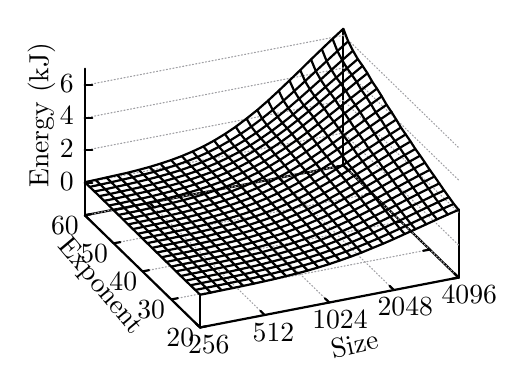
\begin{tikzpicture}[y=0.80pt, x=0.80pt, yscale=-0.570000, xscale=0.570000, inner sep=0pt, outer sep=0pt]
\begin{scope}[draw=black,line join=bevel,line cap=rect,even odd rule,line width=0.800pt]
  \begin{scope}[cm={{1.0,0.0,0.0,1.0,(0.0,0.0)}},draw=black,line join=bevel,line cap=rect,line width=0.800pt]
  \end{scope}
  \begin{scope}[cm={{1.00465,0.0,0.0,1.00465,(0.0,0.0)}},draw=black,line join=bevel,line cap=rect,line width=0.800pt]
  \end{scope}
  \begin{scope}[cm={{1.00465,0.0,0.0,1.00465,(0.0,0.0)}},draw=black,line join=round,line cap=round,line width=0.800pt]
    \path[draw] (67.6000,186.1000) -- (271.5000,146.8000);
    \path[draw] (362.4000,235.2000) -- (271.5000,146.8000);
    \path[draw] (67.5000,186.5000) -- (67.5000,70.5000);
    \path[draw] (271.5000,146.5000) -- (271.5000,39.5000);
    \path[draw] (362.5000,235.5000) -- (362.5000,181.5000);
  \end{scope}
  \begin{scope}[cm={{1.00465,0.0,0.0,1.00465,(0.0,0.0)}},draw=ca0a0a4,dash pattern=on 0.40pt off 0.80pt,line join=round,line cap=round,line width=0.400pt]
    \path[draw] (158.5000,274.6000) -- (67.6000,186.1000);
  \end{scope}
  \begin{scope}[cm={{1.00465,0.0,0.0,1.00465,(0.0,0.0)}},draw=black,line join=round,line cap=round,line width=0.800pt]
    \path[draw] (158.5000,274.6000) -- (155.1000,271.3000);
    \path[draw] (67.6000,186.1000) -- (71.0000,189.4000);
  \end{scope}
  \begin{scope}[cm={{1.00465,0.0,0.0,1.00465,(0.0,0.0)}},draw=black,line join=bevel,line cap=rect,line width=0.800pt]
  \end{scope}
  \begin{scope}[cm={{1.00465,0.0,0.0,1.00465,(149.693,296.874)}},draw=black,line join=bevel,line cap=rect,line width=0.800pt]
  \end{scope}
  \begin{scope}[cm={{1.00465,0.0,0.0,1.00465,(149.693,296.874)}},draw=black,line join=bevel,line cap=rect,line width=0.800pt]
  \end{scope}
  \begin{scope}[cm={{1.00465,0.0,0.0,1.00465,(149.693,296.874)}},draw=black,line join=bevel,line cap=rect,line width=0.800pt]
  \end{scope}
  \begin{scope}[cm={{1.00465,0.0,0.0,1.00465,(149.693,296.874)}},draw=black,line join=bevel,line cap=rect,line width=0.800pt]
  \end{scope}
  \begin{scope}[cm={{1.00465,0.0,0.0,1.00465,(149.693,296.874)}},draw=black,line join=bevel,line cap=rect,line width=0.800pt]
  \end{scope}
  \begin{scope}[cm={{1.00465,0.0,0.0,1.00465,(149.693,296.874)}},draw=black,line join=bevel,line cap=rect,line width=0.800pt]
    \path[fill=black] (0.0000,0.0000) node[above right] () {256};
  \end{scope}
  \begin{scope}[cm={{1.00465,0.0,0.0,1.00465,(149.693,296.874)}},draw=black,line join=bevel,line cap=rect,line width=0.800pt]
  \end{scope}
  \begin{scope}[cm={{1.00465,0.0,0.0,1.00465,(0.0,0.0)}},draw=black,line join=bevel,line cap=rect,line width=0.800pt]
  \end{scope}
  \begin{scope}[cm={{1.00465,0.0,0.0,1.00465,(0.0,0.0)}},draw=ca0a0a4,dash pattern=on 0.40pt off 0.80pt,line join=round,line cap=round,line width=0.400pt]
    \path[draw] (209.5000,264.8000) -- (118.6000,176.3000);
  \end{scope}
  \begin{scope}[cm={{1.00465,0.0,0.0,1.00465,(0.0,0.0)}},draw=black,line join=round,line cap=round,line width=0.800pt]
    \path[draw] (209.5000,264.8000) -- (206.1000,261.5000);
    \path[draw] (118.6000,176.3000) -- (122.0000,179.6000);
  \end{scope}
  \begin{scope}[cm={{1.00465,0.0,0.0,1.00465,(0.0,0.0)}},draw=black,line join=bevel,line cap=rect,line width=0.800pt]
  \end{scope}
  \begin{scope}[cm={{1.00465,0.0,0.0,1.00465,(200.93,286.828)}},draw=black,line join=bevel,line cap=rect,line width=0.800pt]
  \end{scope}
  \begin{scope}[cm={{1.00465,0.0,0.0,1.00465,(200.93,286.828)}},draw=black,line join=bevel,line cap=rect,line width=0.800pt]
  \end{scope}
  \begin{scope}[cm={{1.00465,0.0,0.0,1.00465,(200.93,286.828)}},draw=black,line join=bevel,line cap=rect,line width=0.800pt]
  \end{scope}
  \begin{scope}[cm={{1.00465,0.0,0.0,1.00465,(200.93,286.828)}},draw=black,line join=bevel,line cap=rect,line width=0.800pt]
  \end{scope}
  \begin{scope}[cm={{1.00465,0.0,0.0,1.00465,(200.93,286.828)}},draw=black,line join=bevel,line cap=rect,line width=0.800pt]
  \end{scope}
  \begin{scope}[cm={{1.00465,0.0,0.0,1.00465,(200.93,286.828)}},draw=black,line join=bevel,line cap=rect,line width=0.800pt]
    \path[fill=black] (0.0000,0.0000) node[above right] () {512};
  \end{scope}
  \begin{scope}[cm={{1.00465,0.0,0.0,1.00465,(200.93,286.828)}},draw=black,line join=bevel,line cap=rect,line width=0.800pt]
  \end{scope}
  \begin{scope}[cm={{1.00465,0.0,0.0,1.00465,(0.0,0.0)}},draw=black,line join=bevel,line cap=rect,line width=0.800pt]
  \end{scope}
  \begin{scope}[cm={{1.00465,0.0,0.0,1.00465,(0.0,0.0)}},draw=ca0a0a4,dash pattern=on 0.40pt off 0.80pt,line join=round,line cap=round,line width=0.400pt]
    \path[draw] (260.4000,254.9000) -- (169.6000,166.4000);
  \end{scope}
  \begin{scope}[cm={{1.00465,0.0,0.0,1.00465,(0.0,0.0)}},draw=black,line join=round,line cap=round,line width=0.800pt]
    \path[draw] (260.4000,254.9000) -- (257.0000,251.6000);
    \path[draw] (169.6000,166.4000) -- (173.0000,169.7000);
  \end{scope}
  \begin{scope}[cm={{1.00465,0.0,0.0,1.00465,(0.0,0.0)}},draw=black,line join=bevel,line cap=rect,line width=0.800pt]
  \end{scope}
  \begin{scope}[cm={{1.00465,0.0,0.0,1.00465,(248.149,276.781)}},draw=black,line join=bevel,line cap=rect,line width=0.800pt]
  \end{scope}
  \begin{scope}[cm={{1.00465,0.0,0.0,1.00465,(248.149,276.781)}},draw=black,line join=bevel,line cap=rect,line width=0.800pt]
  \end{scope}
  \begin{scope}[cm={{1.00465,0.0,0.0,1.00465,(248.149,276.781)}},draw=black,line join=bevel,line cap=rect,line width=0.800pt]
  \end{scope}
  \begin{scope}[cm={{1.00465,0.0,0.0,1.00465,(248.149,276.781)}},draw=black,line join=bevel,line cap=rect,line width=0.800pt]
  \end{scope}
  \begin{scope}[cm={{1.00465,0.0,0.0,1.00465,(248.149,276.781)}},draw=black,line join=bevel,line cap=rect,line width=0.800pt]
  \end{scope}
  \begin{scope}[cm={{1.00465,0.0,0.0,1.00465,(248.149,276.781)}},draw=black,line join=bevel,line cap=rect,line width=0.800pt]
    \path[fill=black] (0.0000,0.0000) node[above right] () {1024};
  \end{scope}
  \begin{scope}[cm={{1.00465,0.0,0.0,1.00465,(248.149,276.781)}},draw=black,line join=bevel,line cap=rect,line width=0.800pt]
  \end{scope}
  \begin{scope}[cm={{1.00465,0.0,0.0,1.00465,(0.0,0.0)}},draw=black,line join=bevel,line cap=rect,line width=0.800pt]
  \end{scope}
  \begin{scope}[cm={{1.00465,0.0,0.0,1.00465,(0.0,0.0)}},draw=ca0a0a4,dash pattern=on 0.40pt off 0.80pt,line join=round,line cap=round,line width=0.400pt]
    \path[draw] (311.4000,245.1000) -- (220.5000,156.6000);
  \end{scope}
  \begin{scope}[cm={{1.00465,0.0,0.0,1.00465,(0.0,0.0)}},draw=black,line join=round,line cap=round,line width=0.800pt]
    \path[draw] (311.4000,245.1000) -- (308.0000,241.8000);
    \path[draw] (220.5000,156.6000) -- (223.9000,159.9000);
  \end{scope}
  \begin{scope}[cm={{1.00465,0.0,0.0,1.00465,(0.0,0.0)}},draw=black,line join=bevel,line cap=rect,line width=0.800pt]
  \end{scope}
  \begin{scope}[cm={{1.00465,0.0,0.0,1.00465,(299.888,266.735)}},draw=black,line join=bevel,line cap=rect,line width=0.800pt]
  \end{scope}
  \begin{scope}[cm={{1.00465,0.0,0.0,1.00465,(299.888,266.735)}},draw=black,line join=bevel,line cap=rect,line width=0.800pt]
  \end{scope}
  \begin{scope}[cm={{1.00465,0.0,0.0,1.00465,(299.888,266.735)}},draw=black,line join=bevel,line cap=rect,line width=0.800pt]
  \end{scope}
  \begin{scope}[cm={{1.00465,0.0,0.0,1.00465,(299.888,266.735)}},draw=black,line join=bevel,line cap=rect,line width=0.800pt]
  \end{scope}
  \begin{scope}[cm={{1.00465,0.0,0.0,1.00465,(299.888,266.735)}},draw=black,line join=bevel,line cap=rect,line width=0.800pt]
  \end{scope}
  \begin{scope}[cm={{1.00465,0.0,0.0,1.00465,(299.888,266.735)}},draw=black,line join=bevel,line cap=rect,line width=0.800pt]
    \path[fill=black] (0.0000,0.0000) node[above right] () {2048};
  \end{scope}
  \begin{scope}[cm={{1.00465,0.0,0.0,1.00465,(299.888,266.735)}},draw=black,line join=bevel,line cap=rect,line width=0.800pt]
  \end{scope}
  \begin{scope}[cm={{1.00465,0.0,0.0,1.00465,(0.0,0.0)}},draw=black,line join=bevel,line cap=rect,line width=0.800pt]
  \end{scope}
  \begin{scope}[cm={{1.00465,0.0,0.0,1.00465,(0.0,0.0)}},draw=ca0a0a4,dash pattern=on 0.40pt off 0.80pt,line join=round,line cap=round,line width=0.400pt]
    \path[draw] (362.4000,235.2000) -- (271.5000,146.8000);
  \end{scope}
  \begin{scope}[cm={{1.00465,0.0,0.0,1.00465,(0.0,0.0)}},draw=black,line join=round,line cap=round,line width=0.800pt]
    \path[draw] (362.4000,235.2000) -- (359.0000,231.9000);
    \path[draw] (271.5000,146.8000) -- (274.9000,150.1000);
  \end{scope}
  \begin{scope}[cm={{1.00465,0.0,0.0,1.00465,(0.0,0.0)}},draw=black,line join=bevel,line cap=rect,line width=0.800pt]
  \end{scope}
  \begin{scope}[cm={{1.00465,0.0,0.0,1.00465,(350.623,256.688)}},draw=black,line join=bevel,line cap=rect,line width=0.800pt]
  \end{scope}
  \begin{scope}[cm={{1.00465,0.0,0.0,1.00465,(350.623,256.688)}},draw=black,line join=bevel,line cap=rect,line width=0.800pt]
  \end{scope}
  \begin{scope}[cm={{1.00465,0.0,0.0,1.00465,(350.623,256.688)}},draw=black,line join=bevel,line cap=rect,line width=0.800pt]
  \end{scope}
  \begin{scope}[cm={{1.00465,0.0,0.0,1.00465,(350.623,256.688)}},draw=black,line join=bevel,line cap=rect,line width=0.800pt]
  \end{scope}
  \begin{scope}[cm={{1.00465,0.0,0.0,1.00465,(350.623,256.688)}},draw=black,line join=bevel,line cap=rect,line width=0.800pt]
  \end{scope}
  \begin{scope}[cm={{1.00465,0.0,0.0,1.00465,(350.623,256.688)}},draw=black,line join=bevel,line cap=rect,line width=0.800pt]
    \path[fill=black] (0.0000,0.0000) node[above right] () {4096};
  \end{scope}
  \begin{scope}[cm={{1.00465,0.0,0.0,1.00465,(350.623,256.688)}},draw=black,line join=bevel,line cap=rect,line width=0.800pt]
  \end{scope}
  \begin{scope}[cm={{1.00465,0.0,0.0,1.00465,(0.0,0.0)}},draw=black,line join=bevel,line cap=rect,line width=0.800pt]
  \end{scope}
  \begin{scope}[cm={{1.00465,0.0,0.0,1.00465,(0.0,0.0)}},draw=ca0a0a4,dash pattern=on 0.40pt off 0.80pt,line join=round,line cap=round,line width=0.400pt]
    \path[draw] (158.5000,274.6000) -- (362.4000,235.2000);
  \end{scope}
  \begin{scope}[cm={{1.00465,0.0,0.0,1.00465,(0.0,0.0)}},draw=black,line join=round,line cap=round,line width=0.800pt]
    \path[draw] (158.5000,274.6000) -- (163.6000,273.6000);
    \path[draw] (362.4000,235.2000) -- (357.2000,236.2000);
  \end{scope}
  \begin{scope}[cm={{1.00465,0.0,0.0,1.00465,(0.0,0.0)}},draw=black,line join=bevel,line cap=rect,line width=0.800pt]
  \end{scope}
  \begin{scope}[cm={{1.00465,0.0,0.0,1.00465,(132.614,290.847)}},draw=black,line join=bevel,line cap=rect,line width=0.800pt]
  \end{scope}
  \begin{scope}[cm={{1.00465,0.0,0.0,1.00465,(132.614,290.847)}},draw=black,line join=bevel,line cap=rect,line width=0.800pt]
  \end{scope}
  \begin{scope}[cm={{1.00465,0.0,0.0,1.00465,(132.614,290.847)}},draw=black,line join=bevel,line cap=rect,line width=0.800pt]
  \end{scope}
  \begin{scope}[cm={{1.00465,0.0,0.0,1.00465,(132.614,290.847)}},draw=black,line join=bevel,line cap=rect,line width=0.800pt]
  \end{scope}
  \begin{scope}[cm={{1.00465,0.0,0.0,1.00465,(132.614,290.847)}},draw=black,line join=bevel,line cap=rect,line width=0.800pt]
  \end{scope}
  \begin{scope}[cm={{1.00465,0.0,0.0,1.00465,(132.614,290.847)}},draw=black,line join=bevel,line cap=rect,line width=0.800pt]
    \path[fill=black] (0.0000,0.0000) node[above right] () {20};
  \end{scope}
  \begin{scope}[cm={{1.00465,0.0,0.0,1.00465,(132.614,290.847)}},draw=black,line join=bevel,line cap=rect,line width=0.800pt]
  \end{scope}
  \begin{scope}[cm={{1.00465,0.0,0.0,1.00465,(0.0,0.0)}},draw=black,line join=bevel,line cap=rect,line width=0.800pt]
  \end{scope}
  \begin{scope}[cm={{1.00465,0.0,0.0,1.00465,(0.0,0.0)}},draw=ca0a0a4,dash pattern=on 0.40pt off 0.80pt,line join=round,line cap=round,line width=0.400pt]
    \path[draw] (135.8000,252.5000) -- (339.7000,213.1000);
  \end{scope}
  \begin{scope}[cm={{1.00465,0.0,0.0,1.00465,(0.0,0.0)}},draw=black,line join=round,line cap=round,line width=0.800pt]
    \path[draw] (135.8000,252.5000) -- (140.9000,251.5000);
    \path[draw] (339.7000,213.1000) -- (334.5000,214.1000);
  \end{scope}
  \begin{scope}[cm={{1.00465,0.0,0.0,1.00465,(0.0,0.0)}},draw=black,line join=bevel,line cap=rect,line width=0.800pt]
  \end{scope}
  \begin{scope}[cm={{1.00465,0.0,0.0,1.00465,(109.507,268.744)}},draw=black,line join=bevel,line cap=rect,line width=0.800pt]
  \end{scope}
  \begin{scope}[cm={{1.00465,0.0,0.0,1.00465,(109.507,268.744)}},draw=black,line join=bevel,line cap=rect,line width=0.800pt]
  \end{scope}
  \begin{scope}[cm={{1.00465,0.0,0.0,1.00465,(109.507,268.744)}},draw=black,line join=bevel,line cap=rect,line width=0.800pt]
  \end{scope}
  \begin{scope}[cm={{1.00465,0.0,0.0,1.00465,(109.507,268.744)}},draw=black,line join=bevel,line cap=rect,line width=0.800pt]
  \end{scope}
  \begin{scope}[cm={{1.00465,0.0,0.0,1.00465,(109.507,268.744)}},draw=black,line join=bevel,line cap=rect,line width=0.800pt]
  \end{scope}
  \begin{scope}[cm={{1.00465,0.0,0.0,1.00465,(109.507,268.744)}},draw=black,line join=bevel,line cap=rect,line width=0.800pt]
    \path[fill=black] (0.0000,0.0000) node[above right] () {30};
  \end{scope}
  \begin{scope}[cm={{1.00465,0.0,0.0,1.00465,(109.507,268.744)}},draw=black,line join=bevel,line cap=rect,line width=0.800pt]
  \end{scope}
  \begin{scope}[cm={{1.00465,0.0,0.0,1.00465,(0.0,0.0)}},draw=black,line join=bevel,line cap=rect,line width=0.800pt]
  \end{scope}
  \begin{scope}[cm={{1.00465,0.0,0.0,1.00465,(0.0,0.0)}},draw=ca0a0a4,dash pattern=on 0.40pt off 0.80pt,line join=round,line cap=round,line width=0.400pt]
    \path[draw] (113.1000,230.4000) -- (316.9000,191.0000);
  \end{scope}
  \begin{scope}[cm={{1.00465,0.0,0.0,1.00465,(0.0,0.0)}},draw=black,line join=round,line cap=round,line width=0.800pt]
    \path[draw] (113.1000,230.4000) -- (118.2000,229.4000);
    \path[draw] (316.9000,191.0000) -- (311.8000,192.0000);
  \end{scope}
  \begin{scope}[cm={{1.00465,0.0,0.0,1.00465,(0.0,0.0)}},draw=black,line join=bevel,line cap=rect,line width=0.800pt]
  \end{scope}
  \begin{scope}[cm={{1.00465,0.0,0.0,1.00465,(87.4047,246.642)}},draw=black,line join=bevel,line cap=rect,line width=0.800pt]
  \end{scope}
  \begin{scope}[cm={{1.00465,0.0,0.0,1.00465,(87.4047,246.642)}},draw=black,line join=bevel,line cap=rect,line width=0.800pt]
  \end{scope}
  \begin{scope}[cm={{1.00465,0.0,0.0,1.00465,(87.4047,246.642)}},draw=black,line join=bevel,line cap=rect,line width=0.800pt]
  \end{scope}
  \begin{scope}[cm={{1.00465,0.0,0.0,1.00465,(87.4047,246.642)}},draw=black,line join=bevel,line cap=rect,line width=0.800pt]
  \end{scope}
  \begin{scope}[cm={{1.00465,0.0,0.0,1.00465,(87.4047,246.642)}},draw=black,line join=bevel,line cap=rect,line width=0.800pt]
  \end{scope}
  \begin{scope}[cm={{1.00465,0.0,0.0,1.00465,(87.4047,246.642)}},draw=black,line join=bevel,line cap=rect,line width=0.800pt]
    \path[fill=black] (0.0000,0.0000) node[above right] () {40};
  \end{scope}
  \begin{scope}[cm={{1.00465,0.0,0.0,1.00465,(87.4047,246.642)}},draw=black,line join=bevel,line cap=rect,line width=0.800pt]
  \end{scope}
  \begin{scope}[cm={{1.00465,0.0,0.0,1.00465,(0.0,0.0)}},draw=black,line join=bevel,line cap=rect,line width=0.800pt]
  \end{scope}
  \begin{scope}[cm={{1.00465,0.0,0.0,1.00465,(0.0,0.0)}},draw=ca0a0a4,dash pattern=on 0.40pt off 0.80pt,line join=round,line cap=round,line width=0.400pt]
    \path[draw] (90.3000,208.2000) -- (294.2000,168.8000);
  \end{scope}
  \begin{scope}[cm={{1.00465,0.0,0.0,1.00465,(0.0,0.0)}},draw=black,line join=round,line cap=round,line width=0.800pt]
    \path[draw] (90.3000,208.2000) -- (95.5000,207.3000);
    \path[draw] (294.2000,168.8000) -- (289.1000,169.8000);
  \end{scope}
  \begin{scope}[cm={{1.00465,0.0,0.0,1.00465,(0.0,0.0)}},draw=black,line join=bevel,line cap=rect,line width=0.800pt]
  \end{scope}
  \begin{scope}[cm={{1.00465,0.0,0.0,1.00465,(64.2977,224.54)}},draw=black,line join=bevel,line cap=rect,line width=0.800pt]
  \end{scope}
  \begin{scope}[cm={{1.00465,0.0,0.0,1.00465,(64.2977,224.54)}},draw=black,line join=bevel,line cap=rect,line width=0.800pt]
  \end{scope}
  \begin{scope}[cm={{1.00465,0.0,0.0,1.00465,(64.2977,224.54)}},draw=black,line join=bevel,line cap=rect,line width=0.800pt]
  \end{scope}
  \begin{scope}[cm={{1.00465,0.0,0.0,1.00465,(64.2977,224.54)}},draw=black,line join=bevel,line cap=rect,line width=0.800pt]
  \end{scope}
  \begin{scope}[cm={{1.00465,0.0,0.0,1.00465,(64.2977,224.54)}},draw=black,line join=bevel,line cap=rect,line width=0.800pt]
  \end{scope}
  \begin{scope}[cm={{1.00465,0.0,0.0,1.00465,(64.2977,224.54)}},draw=black,line join=bevel,line cap=rect,line width=0.800pt]
    \path[fill=black] (0.0000,0.0000) node[above right] () {50};
  \end{scope}
  \begin{scope}[cm={{1.00465,0.0,0.0,1.00465,(64.2977,224.54)}},draw=black,line join=bevel,line cap=rect,line width=0.800pt]
  \end{scope}
  \begin{scope}[cm={{1.00465,0.0,0.0,1.00465,(0.0,0.0)}},draw=black,line join=bevel,line cap=rect,line width=0.800pt]
  \end{scope}
  \begin{scope}[cm={{1.00465,0.0,0.0,1.00465,(0.0,0.0)}},draw=ca0a0a4,dash pattern=on 0.40pt off 0.80pt,line join=round,line cap=round,line width=0.400pt]
    \path[draw] (67.6000,186.1000) -- (271.5000,146.8000);
  \end{scope}
  \begin{scope}[cm={{1.00465,0.0,0.0,1.00465,(0.0,0.0)}},draw=black,line join=round,line cap=round,line width=0.800pt]
    \path[draw] (67.6000,186.1000) -- (72.8000,185.1000);
    \path[draw] (271.5000,146.8000) -- (266.4000,147.8000);
  \end{scope}
  \begin{scope}[cm={{1.00465,0.0,0.0,1.00465,(0.0,0.0)}},draw=black,line join=bevel,line cap=rect,line width=0.800pt]
  \end{scope}
  \begin{scope}[cm={{1.00465,0.0,0.0,1.00465,(41.1907,202.437)}},draw=black,line join=bevel,line cap=rect,line width=0.800pt]
  \end{scope}
  \begin{scope}[cm={{1.00465,0.0,0.0,1.00465,(41.1907,202.437)}},draw=black,line join=bevel,line cap=rect,line width=0.800pt]
  \end{scope}
  \begin{scope}[cm={{1.00465,0.0,0.0,1.00465,(41.1907,202.437)}},draw=black,line join=bevel,line cap=rect,line width=0.800pt]
  \end{scope}
  \begin{scope}[cm={{1.00465,0.0,0.0,1.00465,(41.1907,202.437)}},draw=black,line join=bevel,line cap=rect,line width=0.800pt]
  \end{scope}
  \begin{scope}[cm={{1.00465,0.0,0.0,1.00465,(41.1907,202.437)}},draw=black,line join=bevel,line cap=rect,line width=0.800pt]
  \end{scope}
  \begin{scope}[cm={{1.00465,0.0,0.0,1.00465,(41.1907,202.437)}},draw=black,line join=bevel,line cap=rect,line width=0.800pt]
    \path[fill=black] (0.0000,0.0000) node[above right] () {60};
  \end{scope}
  \begin{scope}[cm={{1.00465,0.0,0.0,1.00465,(41.1907,202.437)}},draw=black,line join=bevel,line cap=rect,line width=0.800pt]
  \end{scope}
  \begin{scope}[cm={{1.00465,0.0,0.0,1.00465,(0.0,0.0)}},draw=black,line join=bevel,line cap=rect,line width=0.800pt]
  \end{scope}
  \begin{scope}[cm={{1.00465,0.0,0.0,1.00465,(0.0,0.0)}},draw=ca0a0a4,dash pattern=on 0.40pt off 0.80pt,line join=round,line cap=round,line width=0.400pt]
    \path[draw] (67.6000,160.5000) -- (271.5000,121.2000);
    \path[draw] (271.5000,121.2000) -- (271.5000,121.2000) -- (362.4000,209.6000);
  \end{scope}
  \begin{scope}[cm={{1.00465,0.0,0.0,1.00465,(0.0,0.0)}},draw=black,line join=round,line cap=round,line width=0.800pt]
    \path[draw] (67.5000,160.5000) -- (73.5000,160.5000);
  \end{scope}
  \begin{scope}[cm={{1.00465,0.0,0.0,1.00465,(0.0,0.0)}},draw=black,line join=bevel,line cap=rect,line width=0.800pt]
  \end{scope}
  \begin{scope}[cm={{1.00465,0.0,0.0,1.00465,(48.2233,167.274)}},draw=black,line join=bevel,line cap=rect,line width=0.800pt]
  \end{scope}
  \begin{scope}[cm={{1.00465,0.0,0.0,1.00465,(48.2233,167.274)}},draw=black,line join=bevel,line cap=rect,line width=0.800pt]
  \end{scope}
  \begin{scope}[cm={{1.00465,0.0,0.0,1.00465,(48.2233,167.274)}},draw=black,line join=bevel,line cap=rect,line width=0.800pt]
  \end{scope}
  \begin{scope}[cm={{1.00465,0.0,0.0,1.00465,(48.2233,167.274)}},draw=black,line join=bevel,line cap=rect,line width=0.800pt]
  \end{scope}
  \begin{scope}[cm={{1.00465,0.0,0.0,1.00465,(48.2233,167.274)}},draw=black,line join=bevel,line cap=rect,line width=0.800pt]
  \end{scope}
  \begin{scope}[cm={{1.00465,0.0,0.0,1.00465,(48.2233,167.274)}},draw=black,line join=bevel,line cap=rect,line width=0.800pt]
    \path[fill=black] (0.0000,0.0000) node[above right] () {0};
  \end{scope}
  \begin{scope}[cm={{1.00465,0.0,0.0,1.00465,(48.2233,167.274)}},draw=black,line join=bevel,line cap=rect,line width=0.800pt]
  \end{scope}
  \begin{scope}[cm={{1.00465,0.0,0.0,1.00465,(0.0,0.0)}},draw=black,line join=bevel,line cap=rect,line width=0.800pt]
  \end{scope}
  \begin{scope}[cm={{1.00465,0.0,0.0,1.00465,(0.0,0.0)}},draw=ca0a0a4,dash pattern=on 0.40pt off 0.80pt,line join=round,line cap=round,line width=0.400pt]
    \path[draw] (67.6000,134.9000) -- (271.5000,95.5000);
    \path[draw] (271.5000,95.5000) -- (271.5000,95.5000) -- (362.4000,183.9000);
  \end{scope}
  \begin{scope}[cm={{1.00465,0.0,0.0,1.00465,(0.0,0.0)}},draw=black,line join=round,line cap=round,line width=0.800pt]
    \path[draw] (67.5000,134.5000) -- (73.5000,134.5000);
  \end{scope}
  \begin{scope}[cm={{1.00465,0.0,0.0,1.00465,(0.0,0.0)}},draw=black,line join=bevel,line cap=rect,line width=0.800pt]
  \end{scope}
  \begin{scope}[cm={{1.00465,0.0,0.0,1.00465,(48.2233,141.153)}},draw=black,line join=bevel,line cap=rect,line width=0.800pt]
  \end{scope}
  \begin{scope}[cm={{1.00465,0.0,0.0,1.00465,(48.2233,141.153)}},draw=black,line join=bevel,line cap=rect,line width=0.800pt]
  \end{scope}
  \begin{scope}[cm={{1.00465,0.0,0.0,1.00465,(48.2233,141.153)}},draw=black,line join=bevel,line cap=rect,line width=0.800pt]
  \end{scope}
  \begin{scope}[cm={{1.00465,0.0,0.0,1.00465,(48.2233,141.153)}},draw=black,line join=bevel,line cap=rect,line width=0.800pt]
  \end{scope}
  \begin{scope}[cm={{1.00465,0.0,0.0,1.00465,(48.2233,141.153)}},draw=black,line join=bevel,line cap=rect,line width=0.800pt]
  \end{scope}
  \begin{scope}[cm={{1.00465,0.0,0.0,1.00465,(48.2233,141.153)}},draw=black,line join=bevel,line cap=rect,line width=0.800pt]
    \path[fill=black] (0.0000,0.0000) node[above right] () {2};
  \end{scope}
  \begin{scope}[cm={{1.00465,0.0,0.0,1.00465,(48.2233,141.153)}},draw=black,line join=bevel,line cap=rect,line width=0.800pt]
  \end{scope}
  \begin{scope}[cm={{1.00465,0.0,0.0,1.00465,(0.0,0.0)}},draw=black,line join=bevel,line cap=rect,line width=0.800pt]
  \end{scope}
  \begin{scope}[cm={{1.00465,0.0,0.0,1.00465,(0.0,0.0)}},draw=ca0a0a4,dash pattern=on 0.40pt off 0.80pt,line join=round,line cap=round,line width=0.400pt]
    \path[draw] (67.6000,109.3000) -- (271.5000,69.9000);
    \path[draw] (271.5000,69.9000) -- (271.5000,69.9000) -- (362.4000,158.3000);
  \end{scope}
  \begin{scope}[cm={{1.00465,0.0,0.0,1.00465,(0.0,0.0)}},draw=black,line join=round,line cap=round,line width=0.800pt]
    \path[draw] (67.5000,109.5000) -- (73.5000,109.5000);
  \end{scope}
  \begin{scope}[cm={{1.00465,0.0,0.0,1.00465,(0.0,0.0)}},draw=black,line join=bevel,line cap=rect,line width=0.800pt]
  \end{scope}
  \begin{scope}[cm={{1.00465,0.0,0.0,1.00465,(48.2233,115.033)}},draw=black,line join=bevel,line cap=rect,line width=0.800pt]
  \end{scope}
  \begin{scope}[cm={{1.00465,0.0,0.0,1.00465,(48.2233,115.033)}},draw=black,line join=bevel,line cap=rect,line width=0.800pt]
  \end{scope}
  \begin{scope}[cm={{1.00465,0.0,0.0,1.00465,(48.2233,115.033)}},draw=black,line join=bevel,line cap=rect,line width=0.800pt]
  \end{scope}
  \begin{scope}[cm={{1.00465,0.0,0.0,1.00465,(48.2233,115.033)}},draw=black,line join=bevel,line cap=rect,line width=0.800pt]
  \end{scope}
  \begin{scope}[cm={{1.00465,0.0,0.0,1.00465,(48.2233,115.033)}},draw=black,line join=bevel,line cap=rect,line width=0.800pt]
  \end{scope}
  \begin{scope}[cm={{1.00465,0.0,0.0,1.00465,(48.2233,115.033)}},draw=black,line join=bevel,line cap=rect,line width=0.800pt]
    \path[fill=black] (0.0000,0.0000) node[above right] () {4};
  \end{scope}
  \begin{scope}[cm={{1.00465,0.0,0.0,1.00465,(48.2233,115.033)}},draw=black,line join=bevel,line cap=rect,line width=0.800pt]
  \end{scope}
  \begin{scope}[cm={{1.00465,0.0,0.0,1.00465,(0.0,0.0)}},draw=black,line join=bevel,line cap=rect,line width=0.800pt]
  \end{scope}
  \begin{scope}[cm={{1.00465,0.0,0.0,1.00465,(0.0,0.0)}},draw=ca0a0a4,dash pattern=on 0.40pt off 0.80pt,line join=round,line cap=round,line width=0.400pt]
    \path[draw] (67.6000,83.6000) -- (271.5000,44.2000);
    \path[draw] (271.5000,44.2000) -- (271.5000,44.2000) -- (362.4000,132.7000);
  \end{scope}
  \begin{scope}[cm={{1.00465,0.0,0.0,1.00465,(0.0,0.0)}},draw=black,line join=round,line cap=round,line width=0.800pt]
    \path[draw] (67.5000,83.5000) -- (73.5000,83.5000);
  \end{scope}
  \begin{scope}[cm={{1.00465,0.0,0.0,1.00465,(0.0,0.0)}},draw=black,line join=bevel,line cap=rect,line width=0.800pt]
  \end{scope}
  \begin{scope}[cm={{1.00465,0.0,0.0,1.00465,(48.2233,89.9163)}},draw=black,line join=bevel,line cap=rect,line width=0.800pt]
  \end{scope}
  \begin{scope}[cm={{1.00465,0.0,0.0,1.00465,(48.2233,89.9163)}},draw=black,line join=bevel,line cap=rect,line width=0.800pt]
  \end{scope}
  \begin{scope}[cm={{1.00465,0.0,0.0,1.00465,(48.2233,89.9163)}},draw=black,line join=bevel,line cap=rect,line width=0.800pt]
  \end{scope}
  \begin{scope}[cm={{1.00465,0.0,0.0,1.00465,(48.2233,89.9163)}},draw=black,line join=bevel,line cap=rect,line width=0.800pt]
  \end{scope}
  \begin{scope}[cm={{1.00465,0.0,0.0,1.00465,(48.2233,89.9163)}},draw=black,line join=bevel,line cap=rect,line width=0.800pt]
  \end{scope}
  \begin{scope}[cm={{1.00465,0.0,0.0,1.00465,(48.2233,89.9163)}},draw=black,line join=bevel,line cap=rect,line width=0.800pt]
    \path[fill=black] (0.0000,0.0000) node[above right] () {6};
  \end{scope}
  \begin{scope}[cm={{1.00465,0.0,0.0,1.00465,(48.2233,89.9163)}},draw=black,line join=bevel,line cap=rect,line width=0.800pt]
  \end{scope}
  \begin{scope}[cm={{0.0,-1.00465,1.00465,0.0,(24.614,166.27)}},draw=black,line join=bevel,line cap=rect,line width=0.800pt]
  \end{scope}
  \begin{scope}[cm={{0.0,-1.00465,1.00465,0.0,(24.614,166.27)}},draw=black,line join=bevel,line cap=rect,line width=0.800pt]
  \end{scope}
  \begin{scope}[cm={{0.0,-1.00465,1.00465,0.0,(24.614,166.27)}},draw=black,line join=bevel,line cap=rect,line width=0.800pt]
  \end{scope}
  \begin{scope}[cm={{0.0,-1.00465,1.00465,0.0,(24.614,166.27)}},draw=black,line join=bevel,line cap=rect,line width=0.800pt]
  \end{scope}
  \begin{scope}[cm={{0.0,-1.00465,1.00465,0.0,(24.614,166.27)}},draw=black,line join=bevel,line cap=rect,line width=0.800pt]
  \end{scope}
  \begin{scope}[cm={{0.0,-1.00465,1.00465,0.0,(22.614,165.177)}},draw=black,line join=bevel,line cap=rect,line width=0.800pt]
    \path[fill=black] (0.0000,0.0000) node[above right] () {\rotatebox{90}{Energy (kJ)}};
  \end{scope}
  \begin{scope}[cm={{0.0,-1.00465,1.00465,0.0,(24.614,166.27)}},draw=black,line join=bevel,line cap=rect,line width=0.800pt]
  \end{scope}
  \begin{scope}[cm={{1.00465,0.0,0.0,1.00465,(0.0,0.0)}},draw=black,line join=bevel,line cap=rect,line width=0.800pt]
  \end{scope}
  \begin{scope}[cm={{1.00465,0.0,0.0,1.00465,(0.0,0.0)}},draw=black,line join=bevel,line cap=rect,line width=0.800pt]
  \end{scope}
  \begin{scope}[cm={{1.00465,0.0,0.0,1.00465,(0.0,0.0)}},draw=black,line join=bevel,line cap=rect,line width=0.800pt]
  \end{scope}
  \begin{scope}[cm={{1.00465,0.0,0.0,1.00465,(0.0,0.0)}},draw=black,line join=round,line cap=round,line width=0.800pt]
    \path[draw] (362.4000,181.8000) -- (358.6000,177.1000) -- (358.6000,177.1000) --
      (354.8000,171.8000) -- (354.8000,171.8000) -- (351.0000,166.5000) --
      (351.0000,166.5000) -- (347.2000,161.0000) -- (347.2000,161.0000) --
      (343.4000,155.5000) -- (343.4000,155.5000) -- (339.7000,150.3000) --
      (339.7000,150.3000) -- (335.9000,144.6000) -- (335.9000,144.6000) --
      (332.1000,139.1000) -- (332.1000,139.1000) -- (328.3000,133.8000) --
      (328.3000,133.8000) -- (324.5000,127.9000) -- (324.5000,127.9000) --
      (320.7000,122.3000) -- (320.7000,122.3000) -- (316.9000,116.9000) --
      (316.9000,116.9000) -- (313.2000,110.6000) -- (313.2000,110.6000) --
      (309.4000,104.5000) -- (309.4000,104.5000) -- (305.6000,98.9000) --
      (305.6000,98.9000) -- (301.8000,92.3000) -- (301.8000,92.3000) --
      (298.0000,86.2000) -- (298.0000,86.2000) -- (294.2000,80.6000) --
      (294.2000,80.6000) -- (290.5000,74.1000) -- (290.5000,74.1000) --
      (286.7000,68.3000) -- (286.7000,68.3000) -- (282.9000,62.9000) --
      (282.9000,62.9000) -- (279.1000,56.3000) -- (279.1000,56.3000) --
      (275.3000,48.9000) -- (275.3000,48.9000) -- (271.5000,39.0000);
    \path[draw] (353.9000,185.5000) -- (350.1000,180.9000) -- (350.1000,180.9000) --
      (346.3000,175.7000) -- (346.3000,175.7000) -- (342.5000,170.5000) --
      (342.5000,170.5000) -- (338.7000,165.1000) -- (338.7000,165.1000) --
      (334.9000,159.8000) -- (334.9000,159.8000) -- (331.2000,154.7000) --
      (331.2000,154.7000) -- (327.4000,149.2000) -- (327.4000,149.2000) --
      (323.6000,143.8000) -- (323.6000,143.8000) -- (319.8000,138.6000) --
      (319.8000,138.6000) -- (316.0000,132.9000) -- (316.0000,132.9000) --
      (312.2000,127.5000) -- (312.2000,127.5000) -- (308.4000,122.3000) --
      (308.4000,122.3000) -- (304.7000,116.2000) -- (304.7000,116.2000) --
      (300.9000,110.3000) -- (300.9000,110.3000) -- (297.1000,104.9000) --
      (297.1000,104.9000) -- (293.3000,98.5000) -- (293.3000,98.5000) --
      (289.5000,92.6000) -- (289.5000,92.6000) -- (285.7000,87.2000) --
      (285.7000,87.2000) -- (282.0000,80.9000) -- (282.0000,80.9000) --
      (278.2000,75.3000) -- (278.2000,75.3000) -- (274.4000,70.1000) --
      (274.4000,70.1000) -- (270.6000,63.8000) -- (270.6000,63.8000) --
      (266.8000,56.6000) -- (266.8000,56.6000) -- (263.0000,46.9000);
    \path[draw] (345.4000,189.3000) -- (341.6000,184.8000) -- (341.6000,184.8000) --
      (337.8000,179.7000) -- (337.8000,179.7000) -- (334.0000,174.7000) --
      (334.0000,174.7000) -- (330.2000,169.4000) -- (330.2000,169.4000) --
      (326.4000,164.2000) -- (326.4000,164.2000) -- (322.7000,159.2000) --
      (322.7000,159.2000) -- (318.9000,153.8000) -- (318.9000,153.8000) --
      (315.1000,148.6000) -- (315.1000,148.6000) -- (311.3000,143.6000) --
      (311.3000,143.6000) -- (307.5000,138.1000) -- (307.5000,138.1000) --
      (303.7000,132.8000) -- (303.7000,132.8000) -- (299.9000,127.7000) --
      (299.9000,127.7000) -- (296.2000,121.9000) -- (296.2000,121.9000) --
      (292.4000,116.2000) -- (292.4000,116.2000) -- (288.6000,110.9000) --
      (288.6000,110.9000) -- (284.8000,104.8000) -- (284.8000,104.8000) --
      (281.0000,99.1000) -- (281.0000,99.1000) -- (277.2000,93.9000) --
      (277.2000,93.9000) -- (273.5000,87.9000) -- (273.5000,87.9000) --
      (269.7000,82.5000) -- (269.7000,82.5000) -- (265.9000,77.5000) --
      (265.9000,77.5000) -- (262.1000,71.4000) -- (262.1000,71.4000) --
      (258.3000,64.5000) -- (258.3000,64.5000) -- (254.5000,55.0000);
    \path[draw] (336.9000,193.2000) -- (333.1000,188.7000) -- (333.1000,188.7000) --
      (329.3000,183.8000) -- (329.3000,183.8000) -- (325.5000,178.8000) --
      (325.5000,178.8000) -- (321.7000,173.7000) -- (321.7000,173.7000) --
      (317.9000,168.7000) -- (317.9000,168.7000) -- (314.2000,163.8000) --
      (314.2000,163.8000) -- (310.4000,158.6000) -- (310.4000,158.6000) --
      (306.6000,153.4000) -- (306.6000,153.4000) -- (302.8000,148.7000) --
      (302.8000,148.7000) -- (299.0000,143.3000) -- (299.0000,143.3000) --
      (295.2000,138.2000) -- (295.2000,138.2000) -- (291.4000,133.3000) --
      (291.4000,133.3000) -- (287.7000,127.6000) -- (287.7000,127.6000) --
      (283.9000,122.2000) -- (283.9000,122.2000) -- (280.1000,117.1000) --
      (280.1000,117.1000) -- (276.3000,111.2000) -- (276.3000,111.2000) --
      (272.5000,105.7000) -- (272.5000,105.7000) -- (268.7000,100.7000) --
      (268.7000,100.7000) -- (265.0000,94.9000) -- (265.0000,94.9000) --
      (261.2000,89.7000) -- (261.2000,89.7000) -- (257.4000,84.9000) --
      (257.4000,84.9000) -- (253.6000,79.1000) -- (253.6000,79.1000) --
      (249.8000,72.4000) -- (249.8000,72.4000) -- (246.0000,63.2000);
    \path[draw] (328.4000,197.1000) -- (324.6000,192.7000) -- (324.6000,192.7000) --
      (320.8000,187.9000) -- (320.8000,187.9000) -- (317.0000,183.0000) --
      (317.0000,183.0000) -- (313.2000,178.1000) -- (313.2000,178.1000) --
      (309.4000,173.2000) -- (309.4000,173.2000) -- (305.7000,168.4000) --
      (305.7000,168.4000) -- (301.9000,163.3000) -- (301.9000,163.3000) --
      (298.1000,158.4000) -- (298.1000,158.4000) -- (294.3000,153.6000) --
      (294.3000,153.6000) -- (290.5000,148.6000) -- (290.5000,148.6000) --
      (286.7000,143.6000) -- (286.7000,143.6000) -- (282.9000,138.8000) --
      (282.9000,138.8000) -- (279.2000,133.4000) -- (279.2000,133.4000) --
      (275.4000,128.1000) -- (275.4000,128.1000) -- (271.6000,123.2000) --
      (271.6000,123.2000) -- (267.8000,117.6000) -- (267.8000,117.6000) --
      (264.0000,112.3000) -- (264.0000,112.3000) -- (260.2000,107.4000) --
      (260.2000,107.4000) -- (256.5000,101.9000) -- (256.5000,101.9000) --
      (252.7000,96.9000) -- (252.7000,96.9000) -- (248.9000,92.3000) --
      (248.9000,92.3000) -- (245.1000,86.7000) -- (245.1000,86.7000) --
      (241.3000,80.3000) -- (241.3000,80.3000) -- (237.5000,71.6000);
    \path[draw] (319.9000,200.9000) -- (316.1000,196.6000) -- (316.1000,196.6000) --
      (312.3000,191.9000) -- (312.3000,191.9000) -- (308.5000,187.2000) --
      (308.5000,187.2000) -- (304.7000,182.4000) -- (304.7000,182.4000) --
      (300.9000,177.7000) -- (300.9000,177.7000) -- (297.2000,173.0000) --
      (297.2000,173.0000) -- (293.4000,168.1000) -- (293.4000,168.1000) --
      (289.6000,163.3000) -- (289.6000,163.3000) -- (285.8000,158.7000) --
      (285.8000,158.7000) -- (282.0000,153.7000) -- (282.0000,153.7000) --
      (278.2000,149.0000) -- (278.2000,149.0000) -- (274.4000,144.4000) --
      (274.4000,144.4000) -- (270.7000,139.1000) -- (270.7000,139.1000) --
      (266.9000,134.0000) -- (266.9000,134.0000) -- (263.1000,129.3000) --
      (263.1000,129.3000) -- (259.3000,123.9000) -- (259.3000,123.9000) --
      (255.5000,118.8000) -- (255.5000,118.8000) -- (251.7000,114.1000) --
      (251.7000,114.1000) -- (248.0000,108.8000) -- (248.0000,108.8000) --
      (244.2000,104.0000) -- (244.2000,104.0000) -- (240.4000,99.5000) --
      (240.4000,99.5000) -- (236.6000,94.2000) -- (236.6000,94.2000) --
      (232.8000,88.1000) -- (232.8000,88.1000) -- (229.0000,79.8000);
    \path[draw] (311.4000,204.8000) -- (307.6000,200.5000) -- (307.6000,200.5000) --
      (303.8000,195.9000) -- (303.8000,195.9000) -- (300.0000,191.4000) --
      (300.0000,191.4000) -- (296.2000,186.7000) -- (296.2000,186.7000) --
      (292.4000,182.1000) -- (292.4000,182.1000) -- (288.7000,177.5000) --
      (288.7000,177.5000) -- (284.9000,172.8000) -- (284.9000,172.8000) --
      (281.1000,168.1000) -- (281.1000,168.1000) -- (277.3000,163.6000) --
      (277.3000,163.6000) -- (273.5000,158.8000) -- (273.5000,158.8000) --
      (269.7000,154.2000) -- (269.7000,154.2000) -- (265.9000,149.7000) --
      (265.9000,149.7000) -- (262.2000,144.7000) -- (262.2000,144.7000) --
      (258.4000,139.8000) -- (258.4000,139.8000) -- (254.6000,135.2000) --
      (254.6000,135.2000) -- (250.8000,130.0000) -- (250.8000,130.0000) --
      (247.0000,125.1000) -- (247.0000,125.1000) -- (243.2000,120.6000) --
      (243.2000,120.6000) -- (239.5000,115.5000) -- (239.5000,115.5000) --
      (235.7000,110.9000) -- (235.7000,110.9000) -- (231.9000,106.6000) --
      (231.9000,106.6000) -- (228.1000,101.5000) -- (228.1000,101.5000) --
      (224.3000,95.7000) -- (224.3000,95.7000) -- (220.5000,87.9000);
    \path[draw] (302.9000,208.5000) -- (299.1000,204.3000) -- (299.1000,204.3000) --
      (295.3000,199.8000) -- (295.3000,199.8000) -- (291.5000,195.4000) --
      (291.5000,195.4000) -- (287.7000,190.9000) -- (287.7000,190.9000) --
      (283.9000,186.4000) -- (283.9000,186.4000) -- (280.2000,181.9000) --
      (280.2000,181.9000) -- (276.4000,177.3000) -- (276.4000,177.3000) --
      (272.6000,172.8000) -- (272.6000,172.8000) -- (268.8000,168.4000) --
      (268.8000,168.4000) -- (265.0000,163.8000) -- (265.0000,163.8000) --
      (261.2000,159.3000) -- (261.2000,159.3000) -- (257.4000,154.9000) --
      (257.4000,154.9000) -- (253.7000,150.1000) -- (253.7000,150.1000) --
      (249.9000,145.4000) -- (249.9000,145.4000) -- (246.1000,140.9000) --
      (246.1000,140.9000) -- (242.3000,135.9000) -- (242.3000,135.9000) --
      (238.5000,131.2000) -- (238.5000,131.2000) -- (234.7000,126.8000) --
      (234.7000,126.8000) -- (231.0000,122.0000) -- (231.0000,122.0000) --
      (227.2000,117.5000) -- (227.2000,117.5000) -- (223.4000,113.3000) --
      (223.4000,113.3000) -- (219.6000,108.4000) -- (219.6000,108.4000) --
      (215.8000,103.0000) -- (215.8000,103.0000) -- (212.1000,95.7000);
    \path[draw] (294.4000,212.0000) -- (290.6000,207.9000) -- (290.6000,207.9000) --
      (286.8000,203.6000) -- (286.8000,203.6000) -- (283.0000,199.3000) --
      (283.0000,199.3000) -- (279.2000,194.8000) -- (279.2000,194.8000) --
      (275.4000,190.5000) -- (275.4000,190.5000) -- (271.7000,186.2000) --
      (271.7000,186.2000) -- (267.9000,181.7000) -- (267.9000,181.7000) --
      (264.1000,177.3000) -- (264.1000,177.3000) -- (260.3000,173.0000) --
      (260.3000,173.0000) -- (256.5000,168.5000) -- (256.5000,168.5000) --
      (252.7000,164.1000) -- (252.7000,164.1000) -- (248.9000,159.8000) --
      (248.9000,159.8000) -- (245.2000,155.2000) -- (245.2000,155.2000) --
      (241.4000,150.7000) -- (241.4000,150.7000) -- (237.6000,146.3000) --
      (237.6000,146.3000) -- (233.8000,141.6000) -- (233.8000,141.6000) --
      (230.0000,137.0000) -- (230.0000,137.0000) -- (226.2000,132.7000) --
      (226.2000,132.7000) -- (222.5000,128.1000) -- (222.5000,128.1000) --
      (218.7000,123.7000) -- (218.7000,123.7000) -- (215.0000,119.6000) --
      (215.0000,119.6000) -- (211.2000,115.0000) -- (211.2000,115.0000) --
      (207.4000,109.8000) -- (207.4000,109.8000) -- (203.6000,103.1000);
    \path[draw] (285.9000,215.5000) -- (282.1000,211.4000) -- (282.1000,211.4000) --
      (278.3000,207.2000) -- (278.3000,207.2000) -- (274.5000,202.9000) --
      (274.5000,202.9000) -- (270.7000,198.7000) -- (270.7000,198.7000) --
      (266.9000,194.4000) -- (266.9000,194.4000) -- (263.2000,190.2000) --
      (263.2000,190.2000) -- (259.4000,185.9000) -- (259.4000,185.9000) --
      (255.6000,181.6000) -- (255.6000,181.6000) -- (251.8000,177.4000) --
      (251.8000,177.4000) -- (248.0000,173.0000) -- (248.0000,173.0000) --
      (244.2000,168.8000) -- (244.2000,168.8000) -- (240.4000,164.6000) --
      (240.4000,164.6000) -- (236.7000,160.1000) -- (236.7000,160.1000) --
      (232.9000,155.6000) -- (232.9000,155.6000) -- (229.1000,151.4000) --
      (229.1000,151.4000) -- (225.3000,146.9000) -- (225.3000,146.9000) --
      (221.5000,142.4000) -- (221.5000,142.4000) -- (217.7000,138.2000) --
      (217.7000,138.2000) -- (214.1000,133.8000) -- (214.1000,133.8000) --
      (210.3000,129.6000) -- (210.3000,129.6000) -- (206.5000,125.5000) --
      (206.5000,125.5000) -- (202.7000,121.1000) -- (202.7000,121.1000) --
      (198.9000,116.2000) -- (198.9000,116.2000) -- (195.1000,109.9000);
    \path[draw] (277.4000,218.7000) -- (273.6000,214.7000) -- (273.6000,214.7000) --
      (269.8000,210.5000) -- (269.8000,210.5000) -- (266.0000,206.4000) --
      (266.0000,206.4000) -- (262.2000,202.2000) -- (262.2000,202.2000) --
      (258.4000,198.1000) -- (258.4000,198.1000) -- (254.7000,194.0000) --
      (254.7000,194.0000) -- (250.9000,189.7000) -- (250.9000,189.7000) --
      (247.1000,185.6000) -- (247.1000,185.6000) -- (243.3000,181.5000) --
      (243.3000,181.5000) -- (239.5000,177.2000) -- (239.5000,177.2000) --
      (235.7000,173.1000) -- (235.7000,173.1000) -- (231.9000,168.9000) --
      (231.9000,168.9000) -- (228.2000,164.6000) -- (228.2000,164.6000) --
      (224.4000,160.3000) -- (224.4000,160.3000) -- (220.6000,156.1000) --
      (220.6000,156.1000) -- (216.8000,151.8000) -- (216.8000,151.8000) --
      (213.1000,147.5000) -- (213.1000,147.5000) -- (209.3000,143.4000) --
      (209.3000,143.4000) -- (205.6000,139.1000) -- (205.6000,139.1000) --
      (201.8000,134.9000) -- (201.8000,134.9000) -- (198.0000,131.0000) --
      (198.0000,131.0000) -- (194.2000,126.7000) -- (194.2000,126.7000) --
      (190.4000,122.0000) -- (190.4000,122.0000) -- (186.6000,116.3000);
    \path[draw] (268.9000,221.7000) -- (265.1000,217.8000) -- (265.1000,217.8000) --
      (261.3000,213.7000) -- (261.3000,213.7000) -- (257.5000,209.7000) --
      (257.5000,209.7000) -- (253.7000,205.6000) -- (253.7000,205.6000) --
      (249.9000,201.5000) -- (249.9000,201.5000) -- (246.2000,197.5000) --
      (246.2000,197.5000) -- (242.4000,193.4000) -- (242.4000,193.4000) --
      (238.6000,189.3000) -- (238.6000,189.3000) -- (234.8000,185.2000) --
      (234.8000,185.2000) -- (231.0000,181.1000) -- (231.0000,181.1000) --
      (227.2000,177.0000) -- (227.2000,177.0000) -- (223.4000,173.0000) --
      (223.4000,173.0000) -- (219.7000,168.8000) -- (219.7000,168.8000) --
      (215.9000,164.6000) -- (215.9000,164.6000) -- (212.2000,160.5000) --
      (212.2000,160.5000) -- (208.4000,156.2000) -- (208.4000,156.2000) --
      (204.6000,152.1000) -- (204.6000,152.1000) -- (200.8000,148.1000) --
      (200.8000,148.1000) -- (197.1000,143.9000) -- (197.1000,143.9000) --
      (193.3000,139.9000) -- (193.3000,139.9000) -- (189.5000,136.0000) --
      (189.5000,136.0000) -- (185.7000,131.8000) -- (185.7000,131.8000) --
      (181.9000,127.3000) -- (181.9000,127.3000) -- (178.1000,122.0000);
    \path[draw] (260.4000,224.6000) -- (256.6000,220.6000) -- (256.6000,220.6000) --
      (252.8000,216.7000) -- (252.8000,216.7000) -- (249.0000,212.7000) --
      (249.0000,212.7000) -- (245.2000,208.7000) -- (245.2000,208.7000) --
      (241.4000,204.7000) -- (241.4000,204.7000) -- (237.7000,200.7000) --
      (237.7000,200.7000) -- (233.9000,196.7000) -- (233.9000,196.7000) --
      (230.1000,192.7000) -- (230.1000,192.7000) -- (226.3000,188.7000) --
      (226.3000,188.7000) -- (222.5000,184.7000) -- (222.5000,184.7000) --
      (218.7000,180.7000) -- (218.7000,180.7000) -- (215.0000,176.7000) --
      (215.0000,176.7000) -- (211.3000,172.6000) -- (211.3000,172.6000) --
      (207.5000,168.5000) -- (207.5000,168.5000) -- (203.7000,164.5000) --
      (203.7000,164.5000) -- (199.9000,160.3000) -- (199.9000,160.3000) --
      (196.1000,156.2000) -- (196.1000,156.2000) -- (192.3000,152.3000) --
      (192.3000,152.3000) -- (188.6000,148.3000) -- (188.6000,148.3000) --
      (184.8000,144.3000) -- (184.8000,144.3000) -- (181.0000,140.5000) --
      (181.0000,140.5000) -- (177.2000,136.4000) -- (177.2000,136.4000) --
      (173.4000,132.1000) -- (173.4000,132.1000) -- (169.6000,127.2000);
    \path[draw] (251.9000,227.2000) -- (248.1000,223.3000) -- (248.1000,223.3000) --
      (244.3000,219.4000) -- (244.3000,219.4000) -- (240.5000,215.5000) --
      (240.5000,215.5000) -- (236.7000,211.5000) -- (236.7000,211.5000) --
      (232.9000,207.6000) -- (232.9000,207.6000) -- (229.2000,203.7000) --
      (229.2000,203.7000) -- (225.4000,199.8000) -- (225.4000,199.8000) --
      (221.6000,195.8000) -- (221.6000,195.8000) -- (217.8000,191.9000) --
      (217.8000,191.9000) -- (214.1000,188.0000) -- (214.1000,188.0000) --
      (210.3000,184.0000) -- (210.3000,184.0000) -- (206.6000,180.1000) --
      (206.6000,180.1000) -- (202.8000,176.1000) -- (202.8000,176.1000) --
      (199.0000,172.1000) -- (199.0000,172.1000) -- (195.2000,168.1000) --
      (195.2000,168.1000) -- (191.4000,164.0000) -- (191.4000,164.0000) --
      (187.6000,160.0000) -- (187.6000,160.0000) -- (183.8000,156.1000) --
      (183.8000,156.1000) -- (180.1000,152.2000) -- (180.1000,152.2000) --
      (176.3000,148.3000) -- (176.3000,148.3000) -- (172.5000,144.5000) --
      (172.5000,144.5000) -- (168.7000,140.5000) -- (168.7000,140.5000) --
      (164.9000,136.4000) -- (164.9000,136.4000) -- (161.1000,131.8000);
    \path[draw] (243.4000,229.7000) -- (239.6000,225.8000) -- (239.6000,225.8000) --
      (235.8000,221.9000) -- (235.8000,221.9000) -- (232.0000,218.1000) --
      (232.0000,218.1000) -- (228.2000,214.2000) -- (228.2000,214.2000) --
      (224.4000,210.3000) -- (224.4000,210.3000) -- (220.7000,206.5000) --
      (220.7000,206.5000) -- (216.9000,202.6000) -- (216.9000,202.6000) --
      (213.2000,198.7000) -- (213.2000,198.7000) -- (209.4000,194.8000) --
      (209.4000,194.8000) -- (205.6000,190.9000) -- (205.6000,190.9000) --
      (201.8000,187.1000) -- (201.8000,187.1000) -- (198.1000,183.2000) --
      (198.1000,183.2000) -- (194.3000,179.2000) -- (194.3000,179.2000) --
      (190.5000,175.3000) -- (190.5000,175.3000) -- (186.7000,171.4000) --
      (186.7000,171.4000) -- (182.9000,167.4000) -- (182.9000,167.4000) --
      (179.1000,163.5000) -- (179.1000,163.5000) -- (175.3000,159.6000) --
      (175.3000,159.6000) -- (171.6000,155.7000) -- (171.6000,155.7000) --
      (167.8000,151.9000) -- (167.8000,151.9000) -- (164.0000,148.1000) --
      (164.0000,148.1000) -- (160.2000,144.2000) -- (160.2000,144.2000) --
      (156.4000,140.2000) -- (156.4000,140.2000) -- (152.6000,135.8000);
    \path[draw] (234.9000,232.0000) -- (231.1000,228.1000) -- (231.1000,228.1000) --
      (227.3000,224.3000) -- (227.3000,224.3000) -- (223.5000,220.5000) --
      (223.5000,220.5000) -- (219.7000,216.7000) -- (219.7000,216.7000) --
      (215.9000,212.8000) -- (215.9000,212.8000) -- (212.3000,209.0000) --
      (212.3000,209.0000) -- (208.5000,205.2000) -- (208.5000,205.2000) --
      (204.7000,201.3000) -- (204.7000,201.3000) -- (200.9000,197.5000) --
      (200.9000,197.5000) -- (197.1000,193.7000) -- (197.1000,193.7000) --
      (193.3000,189.8000) -- (193.3000,189.8000) -- (189.6000,186.0000) --
      (189.6000,186.0000) -- (185.8000,182.1000) -- (185.8000,182.1000) --
      (182.0000,178.2000) -- (182.0000,178.2000) -- (178.2000,174.3000) --
      (178.2000,174.3000) -- (174.4000,170.4000) -- (174.4000,170.4000) --
      (170.6000,166.5000) -- (170.6000,166.5000) -- (166.8000,162.7000) --
      (166.8000,162.7000) -- (163.1000,158.8000) -- (163.1000,158.8000) --
      (159.3000,155.0000) -- (159.3000,155.0000) -- (155.5000,151.4000) --
      (155.5000,151.4000) -- (151.7000,147.5000) -- (151.7000,147.5000) --
      (147.9000,143.6000) -- (147.9000,143.6000) -- (144.1000,139.4000);
    \path[draw] (226.4000,234.1000) -- (222.6000,230.3000) -- (222.6000,230.3000) --
      (218.8000,226.5000) -- (218.8000,226.5000) -- (215.0000,222.7000) --
      (215.0000,222.7000) -- (211.3000,219.0000) -- (211.3000,219.0000) --
      (207.5000,215.2000) -- (207.5000,215.2000) -- (203.8000,211.4000) --
      (203.8000,211.4000) -- (200.0000,207.6000) -- (200.0000,207.6000) --
      (196.2000,203.8000) -- (196.2000,203.8000) -- (192.4000,200.0000) --
      (192.4000,200.0000) -- (188.6000,196.2000) -- (188.6000,196.2000) --
      (184.8000,192.4000) -- (184.8000,192.4000) -- (181.1000,188.6000) --
      (181.1000,188.6000) -- (177.3000,184.7000) -- (177.3000,184.7000) --
      (173.5000,180.9000) -- (173.5000,180.9000) -- (169.7000,177.0000) --
      (169.7000,177.0000) -- (165.9000,173.2000) -- (165.9000,173.2000) --
      (162.1000,169.3000) -- (162.1000,169.3000) -- (158.3000,165.5000) --
      (158.3000,165.5000) -- (154.6000,161.7000) -- (154.6000,161.7000) --
      (150.8000,157.9000) -- (150.8000,157.9000) -- (147.0000,154.2000) --
      (147.0000,154.2000) -- (143.2000,150.5000) -- (143.2000,150.5000) --
      (139.4000,146.6000) -- (139.4000,146.6000) -- (135.6000,142.6000);
    \path[draw] (217.9000,236.2000) -- (214.2000,232.4000) -- (214.2000,232.4000) --
      (210.4000,228.6000) -- (210.4000,228.6000) -- (206.6000,224.9000) --
      (206.6000,224.9000) -- (202.8000,221.1000) -- (202.8000,221.1000) --
      (199.0000,217.3000) -- (199.0000,217.3000) -- (195.3000,213.6000) --
      (195.3000,213.6000) -- (191.5000,209.8000) -- (191.5000,209.8000) --
      (187.7000,206.0000) -- (187.7000,206.0000) -- (183.9000,202.3000) --
      (183.9000,202.3000) -- (180.1000,198.5000) -- (180.1000,198.5000) --
      (176.3000,194.7000) -- (176.3000,194.7000) -- (172.6000,190.9000) --
      (172.6000,190.9000) -- (168.8000,187.1000) -- (168.8000,187.1000) --
      (165.0000,183.3000) -- (165.0000,183.3000) -- (161.2000,179.5000) --
      (161.2000,179.5000) -- (157.4000,175.7000) -- (157.4000,175.7000) --
      (153.6000,171.9000) -- (153.6000,171.9000) -- (149.8000,168.1000) --
      (149.8000,168.1000) -- (146.1000,164.3000) -- (146.1000,164.3000) --
      (142.3000,160.6000) -- (142.3000,160.6000) -- (138.5000,156.8000) --
      (138.5000,156.8000) -- (134.7000,153.1000) -- (134.7000,153.1000) --
      (130.9000,149.3000) -- (130.9000,149.3000) -- (127.1000,145.4000);
    \path[draw] (209.5000,238.1000) -- (205.7000,234.4000) -- (205.7000,234.4000) --
      (201.9000,230.6000) -- (201.9000,230.6000) -- (198.1000,226.9000) --
      (198.1000,226.9000) -- (194.3000,223.1000) -- (194.3000,223.1000) --
      (190.5000,219.4000) -- (190.5000,219.4000) -- (186.8000,215.6000) --
      (186.8000,215.6000) -- (183.0000,211.9000) -- (183.0000,211.9000) --
      (179.2000,208.1000) -- (179.2000,208.1000) -- (175.4000,204.4000) --
      (175.4000,204.4000) -- (171.6000,200.6000) -- (171.6000,200.6000) --
      (167.8000,196.9000) -- (167.8000,196.9000) -- (164.1000,193.1000) --
      (164.1000,193.1000) -- (160.3000,189.3000) -- (160.3000,189.3000) --
      (156.5000,185.6000) -- (156.5000,185.6000) -- (152.7000,181.8000) --
      (152.7000,181.8000) -- (148.9000,178.0000) -- (148.9000,178.0000) --
      (145.1000,174.2000) -- (145.1000,174.2000) -- (141.3000,170.5000) --
      (141.3000,170.5000) -- (137.6000,166.7000) -- (137.6000,166.7000) --
      (133.8000,163.0000) -- (133.8000,163.0000) -- (130.0000,159.2000) --
      (130.0000,159.2000) -- (126.2000,155.5000) -- (126.2000,155.5000) --
      (122.4000,151.8000) -- (122.4000,151.8000) -- (118.6000,148.0000);
    \path[draw] (201.0000,240.0000) -- (197.2000,236.3000) -- (197.2000,236.3000) --
      (193.4000,232.5000) -- (193.4000,232.5000) -- (189.6000,228.8000) --
      (189.6000,228.8000) -- (185.8000,225.1000) -- (185.8000,225.1000) --
      (182.0000,221.3000) -- (182.0000,221.3000) -- (178.3000,217.6000) --
      (178.3000,217.6000) -- (174.5000,213.9000) -- (174.5000,213.9000) --
      (170.7000,210.1000) -- (170.7000,210.1000) -- (166.9000,206.4000) --
      (166.9000,206.4000) -- (163.1000,202.7000) -- (163.1000,202.7000) --
      (159.3000,198.9000) -- (159.3000,198.9000) -- (155.6000,195.2000) --
      (155.6000,195.2000) -- (151.8000,191.4000) -- (151.8000,191.4000) --
      (148.0000,187.7000) -- (148.0000,187.7000) -- (144.2000,183.9000) --
      (144.2000,183.9000) -- (140.4000,180.2000) -- (140.4000,180.2000) --
      (136.6000,176.4000) -- (136.6000,176.4000) -- (132.8000,172.7000) --
      (132.8000,172.7000) -- (129.1000,168.9000) -- (129.1000,168.9000) --
      (125.3000,165.2000) -- (125.3000,165.2000) -- (121.5000,161.5000) --
      (121.5000,161.5000) -- (117.7000,157.7000) -- (117.7000,157.7000) --
      (113.9000,154.0000) -- (113.9000,154.0000) -- (110.1000,150.3000);
    \path[draw] (192.5000,241.8000) -- (188.7000,238.1000) -- (188.7000,238.1000) --
      (184.9000,234.4000) -- (184.9000,234.4000) -- (181.1000,230.7000) --
      (181.1000,230.7000) -- (177.3000,226.9000) -- (177.3000,226.9000) --
      (173.5000,223.2000) -- (173.5000,223.2000) -- (169.8000,219.5000) --
      (169.8000,219.5000) -- (166.0000,215.8000) -- (166.0000,215.8000) --
      (162.2000,212.1000) -- (162.2000,212.1000) -- (158.4000,208.3000) --
      (158.4000,208.3000) -- (154.6000,204.6000) -- (154.6000,204.6000) --
      (150.8000,200.9000) -- (150.8000,200.9000) -- (147.1000,197.2000) --
      (147.1000,197.2000) -- (143.3000,193.4000) -- (143.3000,193.4000) --
      (139.5000,189.7000) -- (139.5000,189.7000) -- (135.7000,185.9000) --
      (135.7000,185.9000) -- (131.9000,182.2000) -- (131.9000,182.2000) --
      (128.1000,178.5000) -- (128.1000,178.5000) -- (124.3000,174.7000) --
      (124.3000,174.7000) -- (120.6000,171.0000) -- (120.6000,171.0000) --
      (116.8000,167.3000) -- (116.8000,167.3000) -- (113.0000,163.6000) --
      (113.0000,163.6000) -- (109.2000,159.8000) -- (109.2000,159.8000) --
      (105.4000,156.1000) -- (105.4000,156.1000) -- (101.6000,152.5000);
    \path[draw] (184.0000,243.6000) -- (180.2000,239.9000) -- (180.2000,239.9000) --
      (176.4000,236.2000) -- (176.4000,236.2000) -- (172.6000,232.5000) --
      (172.6000,232.5000) -- (168.8000,228.7000) -- (168.8000,228.7000) --
      (165.0000,225.0000) -- (165.0000,225.0000) -- (161.3000,221.3000) --
      (161.3000,221.3000) -- (157.5000,217.6000) -- (157.5000,217.6000) --
      (153.7000,213.9000) -- (153.7000,213.9000) -- (149.9000,210.2000) --
      (149.9000,210.2000) -- (146.1000,206.5000) -- (146.1000,206.5000) --
      (142.3000,202.8000) -- (142.3000,202.8000) -- (138.6000,199.0000) --
      (138.6000,199.0000) -- (134.8000,195.3000) -- (134.8000,195.3000) --
      (131.0000,191.6000) -- (131.0000,191.6000) -- (127.2000,187.9000) --
      (127.2000,187.9000) -- (123.4000,184.1000) -- (123.4000,184.1000) --
      (119.6000,180.4000) -- (119.6000,180.4000) -- (115.8000,176.7000) --
      (115.8000,176.7000) -- (112.1000,173.0000) -- (112.1000,173.0000) --
      (108.3000,169.2000) -- (108.3000,169.2000) -- (104.5000,165.5000) --
      (104.5000,165.5000) -- (100.7000,161.8000) -- (100.7000,161.8000) --
      (96.9000,158.1000) -- (96.9000,158.1000) -- (93.1000,154.4000);
    \path[draw] (175.5000,245.3000) -- (171.7000,241.6000) -- (171.7000,241.6000) --
      (167.9000,237.9000) -- (167.9000,237.9000) -- (164.1000,234.2000) --
      (164.1000,234.2000) -- (160.3000,230.5000) -- (160.3000,230.5000) --
      (156.5000,226.8000) -- (156.5000,226.8000) -- (152.8000,223.1000) --
      (152.8000,223.1000) -- (149.0000,219.4000) -- (149.0000,219.4000) --
      (145.2000,215.7000) -- (145.2000,215.7000) -- (141.4000,212.0000) --
      (141.4000,212.0000) -- (137.6000,208.3000) -- (137.6000,208.3000) --
      (133.8000,204.6000) -- (133.8000,204.6000) -- (130.1000,200.9000) --
      (130.1000,200.9000) -- (126.3000,197.1000) -- (126.3000,197.1000) --
      (122.5000,193.4000) -- (122.5000,193.4000) -- (118.7000,189.7000) --
      (118.7000,189.7000) -- (114.9000,186.0000) -- (114.9000,186.0000) --
      (111.1000,182.3000) -- (111.1000,182.3000) -- (107.3000,178.5000) --
      (107.3000,178.5000) -- (103.6000,174.8000) -- (103.6000,174.8000) --
      (99.8000,171.1000) -- (99.8000,171.1000) -- (96.0000,167.4000) --
      (96.0000,167.4000) -- (92.2000,163.7000) -- (92.2000,163.7000) --
      (88.4000,160.0000) -- (88.4000,160.0000) -- (84.6000,156.3000);
    \path[draw] (167.0000,247.1000) -- (163.2000,243.3000) -- (163.2000,243.3000) --
      (159.4000,239.6000) -- (159.4000,239.6000) -- (155.6000,235.9000) --
      (155.6000,235.9000) -- (151.8000,232.2000) -- (151.8000,232.2000) --
      (148.0000,228.6000) -- (148.0000,228.6000) -- (144.3000,224.8000) --
      (144.3000,224.8000) -- (140.5000,221.1000) -- (140.5000,221.1000) --
      (136.7000,217.4000) -- (136.7000,217.4000) -- (132.9000,213.7000) --
      (132.9000,213.7000) -- (129.1000,210.0000) -- (129.1000,210.0000) --
      (125.3000,206.3000) -- (125.3000,206.3000) -- (121.6000,202.6000) --
      (121.6000,202.6000) -- (117.8000,198.9000) -- (117.8000,198.9000) --
      (114.0000,195.2000) -- (114.0000,195.2000) -- (110.2000,191.5000) --
      (110.2000,191.5000) -- (106.4000,187.8000) -- (106.4000,187.8000) --
      (102.6000,184.1000) -- (102.6000,184.1000) -- (98.8000,180.4000) --
      (98.8000,180.4000) -- (95.1000,176.7000) -- (95.1000,176.7000) --
      (91.3000,173.0000) -- (91.3000,173.0000) -- (87.5000,169.3000) --
      (87.5000,169.3000) -- (83.7000,165.6000) -- (83.7000,165.6000) --
      (79.9000,161.9000) -- (79.9000,161.9000) -- (76.1000,158.2000);
    \path[draw] (158.5000,248.8000) -- (154.7000,245.0000) -- (154.7000,245.0000) --
      (150.9000,241.3000) -- (150.9000,241.3000) -- (147.1000,237.7000) --
      (147.1000,237.7000) -- (143.3000,234.0000) -- (143.3000,234.0000) --
      (139.5000,230.3000) -- (139.5000,230.3000) -- (135.8000,226.6000) --
      (135.8000,226.6000) -- (132.0000,222.9000) -- (132.0000,222.9000) --
      (128.2000,219.2000) -- (128.2000,219.2000) -- (124.4000,215.5000) --
      (124.4000,215.5000) -- (120.6000,211.8000) -- (120.6000,211.8000) --
      (116.8000,208.1000) -- (116.8000,208.1000) -- (113.1000,204.4000) --
      (113.1000,204.4000) -- (109.3000,200.7000) -- (109.3000,200.7000) --
      (105.5000,197.0000) -- (105.5000,197.0000) -- (101.7000,193.3000) --
      (101.7000,193.3000) -- (97.9000,189.5000) -- (97.9000,189.5000) --
      (94.1000,185.8000) -- (94.1000,185.8000) -- (90.3000,182.1000) --
      (90.3000,182.1000) -- (86.6000,178.4000) -- (86.6000,178.4000) --
      (82.8000,174.7000) -- (82.8000,174.7000) -- (79.0000,171.0000) --
      (79.0000,171.0000) -- (75.2000,167.3000) -- (75.2000,167.3000) --
      (71.4000,163.7000) -- (71.4000,163.7000) -- (67.6000,160.0000);
    \path[draw] (271.5000,39.0000) -- (263.0000,46.9000) -- (263.0000,46.9000) --
      (254.5000,55.0000) -- (254.5000,55.0000) -- (246.0000,63.2000) --
      (246.0000,63.2000) -- (237.5000,71.6000) -- (237.5000,71.6000) --
      (229.0000,79.8000) -- (229.0000,79.8000) -- (220.5000,87.9000) --
      (220.5000,87.9000) -- (212.1000,95.7000) -- (212.1000,95.7000) --
      (203.6000,103.1000) -- (203.6000,103.1000) -- (195.1000,109.9000) --
      (195.1000,109.9000) -- (186.6000,116.3000) -- (186.6000,116.3000) --
      (178.1000,122.0000) -- (178.1000,122.0000) -- (169.6000,127.2000) --
      (169.6000,127.2000) -- (161.1000,131.8000) -- (161.1000,131.8000) --
      (152.6000,135.8000) -- (152.6000,135.8000) -- (144.1000,139.4000) --
      (144.1000,139.4000) -- (135.6000,142.6000) -- (135.6000,142.6000) --
      (127.1000,145.4000) -- (127.1000,145.4000) -- (118.6000,148.0000) --
      (118.6000,148.0000) -- (110.1000,150.3000) -- (110.1000,150.3000) --
      (101.6000,152.5000) -- (101.6000,152.5000) -- (93.1000,154.4000) --
      (93.1000,154.4000) -- (84.6000,156.3000) -- (84.6000,156.3000) --
      (76.1000,158.2000) -- (76.1000,158.2000) -- (67.6000,160.0000);
    \path[draw] (275.3000,48.9000) -- (266.8000,56.6000) -- (266.8000,56.6000) --
      (258.3000,64.5000) -- (258.3000,64.5000) -- (249.8000,72.4000) --
      (249.8000,72.4000) -- (241.3000,80.3000) -- (241.3000,80.3000) --
      (232.8000,88.1000) -- (232.8000,88.1000) -- (224.3000,95.7000) --
      (224.3000,95.7000) -- (215.8000,103.0000) -- (215.8000,103.0000) --
      (207.4000,109.8000) -- (207.4000,109.8000) -- (198.9000,116.2000) --
      (198.9000,116.2000) -- (190.4000,122.0000) -- (190.4000,122.0000) --
      (181.9000,127.3000) -- (181.9000,127.3000) -- (173.4000,132.1000) --
      (173.4000,132.1000) -- (164.9000,136.4000) -- (164.9000,136.4000) --
      (156.4000,140.2000) -- (156.4000,140.2000) -- (147.9000,143.6000) --
      (147.9000,143.6000) -- (139.4000,146.6000) -- (139.4000,146.6000) --
      (130.9000,149.3000) -- (130.9000,149.3000) -- (122.4000,151.8000) --
      (122.4000,151.8000) -- (113.9000,154.0000) -- (113.9000,154.0000) --
      (105.4000,156.1000) -- (105.4000,156.1000) -- (96.9000,158.1000) --
      (96.9000,158.1000) -- (88.4000,160.0000) -- (88.4000,160.0000) --
      (79.9000,161.9000) -- (79.9000,161.9000) -- (71.4000,163.7000);
    \path[draw] (279.1000,56.3000) -- (270.6000,63.8000) -- (270.6000,63.8000) --
      (262.1000,71.4000) -- (262.1000,71.4000) -- (253.6000,79.1000) --
      (253.6000,79.1000) -- (245.1000,86.7000) -- (245.1000,86.7000) --
      (236.6000,94.2000) -- (236.6000,94.2000) -- (228.1000,101.5000) --
      (228.1000,101.5000) -- (219.6000,108.4000) -- (219.6000,108.4000) --
      (211.2000,115.0000) -- (211.2000,115.0000) -- (202.7000,121.1000) --
      (202.7000,121.1000) -- (194.2000,126.7000) -- (194.2000,126.7000) --
      (185.7000,131.8000) -- (185.7000,131.8000) -- (177.2000,136.4000) --
      (177.2000,136.4000) -- (168.7000,140.5000) -- (168.7000,140.5000) --
      (160.2000,144.2000) -- (160.2000,144.2000) -- (151.7000,147.5000) --
      (151.7000,147.5000) -- (143.2000,150.5000) -- (143.2000,150.5000) --
      (134.7000,153.1000) -- (134.7000,153.1000) -- (126.2000,155.5000) --
      (126.2000,155.5000) -- (117.7000,157.7000) -- (117.7000,157.7000) --
      (109.2000,159.8000) -- (109.2000,159.8000) -- (100.7000,161.8000) --
      (100.7000,161.8000) -- (92.2000,163.7000) -- (92.2000,163.7000) --
      (83.7000,165.6000) -- (83.7000,165.6000) -- (75.2000,167.3000);
    \path[draw] (282.9000,62.9000) -- (274.4000,70.1000) -- (274.4000,70.1000) --
      (265.9000,77.5000) -- (265.9000,77.5000) -- (257.4000,84.9000) --
      (257.4000,84.9000) -- (248.9000,92.3000) -- (248.9000,92.3000) --
      (240.4000,99.5000) -- (240.4000,99.5000) -- (231.9000,106.6000) --
      (231.9000,106.6000) -- (223.4000,113.3000) -- (223.4000,113.3000) --
      (215.0000,119.6000) -- (215.0000,119.6000) -- (206.5000,125.5000) --
      (206.5000,125.5000) -- (198.0000,131.0000) -- (198.0000,131.0000) --
      (189.5000,136.0000) -- (189.5000,136.0000) -- (181.0000,140.5000) --
      (181.0000,140.5000) -- (172.5000,144.5000) -- (172.5000,144.5000) --
      (164.0000,148.1000) -- (164.0000,148.1000) -- (155.5000,151.4000) --
      (155.5000,151.4000) -- (147.0000,154.2000) -- (147.0000,154.2000) --
      (138.5000,156.8000) -- (138.5000,156.8000) -- (130.0000,159.2000) --
      (130.0000,159.2000) -- (121.5000,161.5000) -- (121.5000,161.5000) --
      (113.0000,163.6000) -- (113.0000,163.6000) -- (104.5000,165.5000) --
      (104.5000,165.5000) -- (96.0000,167.4000) -- (96.0000,167.4000) --
      (87.5000,169.3000) -- (87.5000,169.3000) -- (79.0000,171.0000);
    \path[draw] (286.7000,68.3000) -- (278.2000,75.3000) -- (278.2000,75.3000) --
      (269.7000,82.5000) -- (269.7000,82.5000) -- (261.2000,89.7000) --
      (261.2000,89.7000) -- (252.7000,96.9000) -- (252.7000,96.9000) --
      (244.2000,104.0000) -- (244.2000,104.0000) -- (235.7000,110.9000) --
      (235.7000,110.9000) -- (227.2000,117.5000) -- (227.2000,117.5000) --
      (218.7000,123.7000) -- (218.7000,123.7000) -- (210.3000,129.6000) --
      (210.3000,129.6000) -- (201.8000,134.9000) -- (201.8000,134.9000) --
      (193.3000,139.9000) -- (193.3000,139.9000) -- (184.8000,144.3000) --
      (184.8000,144.3000) -- (176.3000,148.3000) -- (176.3000,148.3000) --
      (167.8000,151.9000) -- (167.8000,151.9000) -- (159.3000,155.0000) --
      (159.3000,155.0000) -- (150.8000,157.9000) -- (150.8000,157.9000) --
      (142.3000,160.6000) -- (142.3000,160.6000) -- (133.8000,163.0000) --
      (133.8000,163.0000) -- (125.3000,165.2000) -- (125.3000,165.2000) --
      (116.8000,167.3000) -- (116.8000,167.3000) -- (108.3000,169.2000) --
      (108.3000,169.2000) -- (99.8000,171.1000) -- (99.8000,171.1000) --
      (91.3000,173.0000) -- (91.3000,173.0000) -- (82.8000,174.7000);
    \path[draw] (290.5000,74.1000) -- (282.0000,80.9000) -- (282.0000,80.9000) --
      (273.5000,87.9000) -- (273.5000,87.9000) -- (265.0000,94.9000) --
      (265.0000,94.9000) -- (256.5000,101.9000) -- (256.5000,101.9000) --
      (248.0000,108.8000) -- (248.0000,108.8000) -- (239.5000,115.5000) --
      (239.5000,115.5000) -- (231.0000,122.0000) -- (231.0000,122.0000) --
      (222.5000,128.1000) -- (222.5000,128.1000) -- (214.1000,133.8000) --
      (214.1000,133.8000) -- (205.6000,139.1000) -- (205.6000,139.1000) --
      (197.1000,143.9000) -- (197.1000,143.9000) -- (188.6000,148.3000) --
      (188.6000,148.3000) -- (180.1000,152.2000) -- (180.1000,152.2000) --
      (171.6000,155.7000) -- (171.6000,155.7000) -- (163.1000,158.8000) --
      (163.1000,158.8000) -- (154.6000,161.7000) -- (154.6000,161.7000) --
      (146.1000,164.3000) -- (146.1000,164.3000) -- (137.6000,166.7000) --
      (137.6000,166.7000) -- (129.1000,168.9000) -- (129.1000,168.9000) --
      (120.6000,171.0000) -- (120.6000,171.0000) -- (112.1000,173.0000) --
      (112.1000,173.0000) -- (103.6000,174.8000) -- (103.6000,174.8000) --
      (95.1000,176.7000) -- (95.1000,176.7000) -- (86.6000,178.4000);
    \path[draw] (294.2000,80.6000) -- (285.7000,87.2000) -- (285.7000,87.2000) --
      (277.2000,93.9000) -- (277.2000,93.9000) -- (268.7000,100.7000) --
      (268.7000,100.7000) -- (260.2000,107.4000) -- (260.2000,107.4000) --
      (251.7000,114.1000) -- (251.7000,114.1000) -- (243.2000,120.6000) --
      (243.2000,120.6000) -- (234.7000,126.8000) -- (234.7000,126.8000) --
      (226.2000,132.7000) -- (226.2000,132.7000) -- (217.7000,138.2000) --
      (217.7000,138.2000) -- (209.3000,143.4000) -- (209.3000,143.4000) --
      (200.8000,148.1000) -- (200.8000,148.1000) -- (192.3000,152.3000) --
      (192.3000,152.3000) -- (183.8000,156.1000) -- (183.8000,156.1000) --
      (175.3000,159.6000) -- (175.3000,159.6000) -- (166.8000,162.7000) --
      (166.8000,162.7000) -- (158.3000,165.5000) -- (158.3000,165.5000) --
      (149.8000,168.1000) -- (149.8000,168.1000) -- (141.3000,170.5000) --
      (141.3000,170.5000) -- (132.8000,172.7000) -- (132.8000,172.7000) --
      (124.3000,174.7000) -- (124.3000,174.7000) -- (115.8000,176.7000) --
      (115.8000,176.7000) -- (107.3000,178.5000) -- (107.3000,178.5000) --
      (98.8000,180.4000) -- (98.8000,180.4000) -- (90.3000,182.1000);
    \path[draw] (298.0000,86.2000) -- (289.5000,92.6000) -- (289.5000,92.6000) --
      (281.0000,99.1000) -- (281.0000,99.1000) -- (272.5000,105.7000) --
      (272.5000,105.7000) -- (264.0000,112.3000) -- (264.0000,112.3000) --
      (255.5000,118.8000) -- (255.5000,118.8000) -- (247.0000,125.1000) --
      (247.0000,125.1000) -- (238.5000,131.2000) -- (238.5000,131.2000) --
      (230.0000,137.0000) -- (230.0000,137.0000) -- (221.5000,142.4000) --
      (221.5000,142.4000) -- (213.1000,147.5000) -- (213.1000,147.5000) --
      (204.6000,152.1000) -- (204.6000,152.1000) -- (196.1000,156.2000) --
      (196.1000,156.2000) -- (187.6000,160.0000) -- (187.6000,160.0000) --
      (179.1000,163.5000) -- (179.1000,163.5000) -- (170.6000,166.5000) --
      (170.6000,166.5000) -- (162.1000,169.3000) -- (162.1000,169.3000) --
      (153.6000,171.9000) -- (153.6000,171.9000) -- (145.1000,174.2000) --
      (145.1000,174.2000) -- (136.6000,176.4000) -- (136.6000,176.4000) --
      (128.1000,178.5000) -- (128.1000,178.5000) -- (119.6000,180.4000) --
      (119.6000,180.4000) -- (111.1000,182.3000) -- (111.1000,182.3000) --
      (102.6000,184.1000) -- (102.6000,184.1000) -- (94.1000,185.8000);
    \path[draw] (301.8000,92.3000) -- (293.3000,98.5000) -- (293.3000,98.5000) --
      (284.8000,104.8000) -- (284.8000,104.8000) -- (276.3000,111.2000) --
      (276.3000,111.2000) -- (267.8000,117.6000) -- (267.8000,117.6000) --
      (259.3000,123.9000) -- (259.3000,123.9000) -- (250.8000,130.0000) --
      (250.8000,130.0000) -- (242.3000,135.9000) -- (242.3000,135.9000) --
      (233.8000,141.6000) -- (233.8000,141.6000) -- (225.3000,146.9000) --
      (225.3000,146.9000) -- (216.8000,151.8000) -- (216.8000,151.8000) --
      (208.4000,156.2000) -- (208.4000,156.2000) -- (199.9000,160.3000) --
      (199.9000,160.3000) -- (191.4000,164.0000) -- (191.4000,164.0000) --
      (182.9000,167.4000) -- (182.9000,167.4000) -- (174.4000,170.4000) --
      (174.4000,170.4000) -- (165.9000,173.2000) -- (165.9000,173.2000) --
      (157.4000,175.7000) -- (157.4000,175.7000) -- (148.9000,178.0000) --
      (148.9000,178.0000) -- (140.4000,180.2000) -- (140.4000,180.2000) --
      (131.9000,182.2000) -- (131.9000,182.2000) -- (123.4000,184.1000) --
      (123.4000,184.1000) -- (114.9000,186.0000) -- (114.9000,186.0000) --
      (106.4000,187.8000) -- (106.4000,187.8000) -- (97.9000,189.5000);
    \path[draw] (305.6000,98.9000) -- (297.1000,104.9000) -- (297.1000,104.9000) --
      (288.6000,110.9000) -- (288.6000,110.9000) -- (280.1000,117.1000) --
      (280.1000,117.1000) -- (271.6000,123.2000) -- (271.6000,123.2000) --
      (263.1000,129.3000) -- (263.1000,129.3000) -- (254.6000,135.2000) --
      (254.6000,135.2000) -- (246.1000,140.9000) -- (246.1000,140.9000) --
      (237.6000,146.3000) -- (237.6000,146.3000) -- (229.1000,151.4000) --
      (229.1000,151.4000) -- (220.6000,156.1000) -- (220.6000,156.1000) --
      (212.2000,160.5000) -- (212.2000,160.5000) -- (203.7000,164.5000) --
      (203.7000,164.5000) -- (195.2000,168.1000) -- (195.2000,168.1000) --
      (186.7000,171.4000) -- (186.7000,171.4000) -- (178.2000,174.3000) --
      (178.2000,174.3000) -- (169.7000,177.0000) -- (169.7000,177.0000) --
      (161.2000,179.5000) -- (161.2000,179.5000) -- (152.7000,181.8000) --
      (152.7000,181.8000) -- (144.2000,183.9000) -- (144.2000,183.9000) --
      (135.7000,185.9000) -- (135.7000,185.9000) -- (127.2000,187.9000) --
      (127.2000,187.9000) -- (118.7000,189.7000) -- (118.7000,189.7000) --
      (110.2000,191.5000) -- (110.2000,191.5000) -- (101.7000,193.3000);
    \path[draw] (309.4000,104.5000) -- (300.9000,110.3000) -- (300.9000,110.3000) --
      (292.4000,116.2000) -- (292.4000,116.2000) -- (283.9000,122.2000) --
      (283.9000,122.2000) -- (275.4000,128.1000) -- (275.4000,128.1000) --
      (266.9000,134.0000) -- (266.9000,134.0000) -- (258.4000,139.8000) --
      (258.4000,139.8000) -- (249.9000,145.4000) -- (249.9000,145.4000) --
      (241.4000,150.7000) -- (241.4000,150.7000) -- (232.9000,155.6000) --
      (232.9000,155.6000) -- (224.4000,160.3000) -- (224.4000,160.3000) --
      (215.9000,164.6000) -- (215.9000,164.6000) -- (207.5000,168.5000) --
      (207.5000,168.5000) -- (199.0000,172.1000) -- (199.0000,172.1000) --
      (190.5000,175.3000) -- (190.5000,175.3000) -- (182.0000,178.2000) --
      (182.0000,178.2000) -- (173.5000,180.9000) -- (173.5000,180.9000) --
      (165.0000,183.3000) -- (165.0000,183.3000) -- (156.5000,185.6000) --
      (156.5000,185.6000) -- (148.0000,187.7000) -- (148.0000,187.7000) --
      (139.5000,189.7000) -- (139.5000,189.7000) -- (131.0000,191.6000) --
      (131.0000,191.6000) -- (122.5000,193.4000) -- (122.5000,193.4000) --
      (114.0000,195.2000) -- (114.0000,195.2000) -- (105.5000,197.0000);
    \path[draw] (313.2000,110.6000) -- (304.7000,116.2000) -- (304.7000,116.2000) --
      (296.2000,121.9000) -- (296.2000,121.9000) -- (287.7000,127.6000) --
      (287.7000,127.6000) -- (279.2000,133.4000) -- (279.2000,133.4000) --
      (270.7000,139.1000) -- (270.7000,139.1000) -- (262.2000,144.7000) --
      (262.2000,144.7000) -- (253.7000,150.1000) -- (253.7000,150.1000) --
      (245.2000,155.2000) -- (245.2000,155.2000) -- (236.7000,160.1000) --
      (236.7000,160.1000) -- (228.2000,164.6000) -- (228.2000,164.6000) --
      (219.7000,168.8000) -- (219.7000,168.8000) -- (211.3000,172.6000) --
      (211.3000,172.6000) -- (202.8000,176.1000) -- (202.8000,176.1000) --
      (194.3000,179.2000) -- (194.3000,179.2000) -- (185.8000,182.1000) --
      (185.8000,182.1000) -- (177.3000,184.7000) -- (177.3000,184.7000) --
      (168.8000,187.1000) -- (168.8000,187.1000) -- (160.3000,189.3000) --
      (160.3000,189.3000) -- (151.8000,191.4000) -- (151.8000,191.4000) --
      (143.3000,193.4000) -- (143.3000,193.4000) -- (134.8000,195.3000) --
      (134.8000,195.3000) -- (126.3000,197.1000) -- (126.3000,197.1000) --
      (117.8000,198.9000) -- (117.8000,198.9000) -- (109.3000,200.7000);
    \path[draw] (316.9000,116.9000) -- (308.4000,122.3000) -- (308.4000,122.3000) --
      (299.9000,127.7000) -- (299.9000,127.7000) -- (291.4000,133.3000) --
      (291.4000,133.3000) -- (282.9000,138.8000) -- (282.9000,138.8000) --
      (274.4000,144.4000) -- (274.4000,144.4000) -- (265.9000,149.7000) --
      (265.9000,149.7000) -- (257.4000,154.9000) -- (257.4000,154.9000) --
      (248.9000,159.8000) -- (248.9000,159.8000) -- (240.4000,164.6000) --
      (240.4000,164.6000) -- (231.9000,168.9000) -- (231.9000,168.9000) --
      (223.4000,173.0000) -- (223.4000,173.0000) -- (215.0000,176.7000) --
      (215.0000,176.7000) -- (206.6000,180.1000) -- (206.6000,180.1000) --
      (198.1000,183.2000) -- (198.1000,183.2000) -- (189.6000,186.0000) --
      (189.6000,186.0000) -- (181.1000,188.6000) -- (181.1000,188.6000) --
      (172.6000,190.9000) -- (172.6000,190.9000) -- (164.1000,193.1000) --
      (164.1000,193.1000) -- (155.6000,195.2000) -- (155.6000,195.2000) --
      (147.1000,197.2000) -- (147.1000,197.2000) -- (138.6000,199.0000) --
      (138.6000,199.0000) -- (130.1000,200.9000) -- (130.1000,200.9000) --
      (121.6000,202.6000) -- (121.6000,202.6000) -- (113.1000,204.4000);
    \path[draw] (320.7000,122.3000) -- (312.2000,127.5000) -- (312.2000,127.5000) --
      (303.7000,132.8000) -- (303.7000,132.8000) -- (295.2000,138.2000) --
      (295.2000,138.2000) -- (286.7000,143.6000) -- (286.7000,143.6000) --
      (278.2000,149.0000) -- (278.2000,149.0000) -- (269.7000,154.2000) --
      (269.7000,154.2000) -- (261.2000,159.3000) -- (261.2000,159.3000) --
      (252.7000,164.1000) -- (252.7000,164.1000) -- (244.2000,168.8000) --
      (244.2000,168.8000) -- (235.7000,173.1000) -- (235.7000,173.1000) --
      (227.2000,177.0000) -- (227.2000,177.0000) -- (218.7000,180.7000) --
      (218.7000,180.7000) -- (210.3000,184.0000) -- (210.3000,184.0000) --
      (201.8000,187.1000) -- (201.8000,187.1000) -- (193.3000,189.8000) --
      (193.3000,189.8000) -- (184.8000,192.4000) -- (184.8000,192.4000) --
      (176.3000,194.7000) -- (176.3000,194.7000) -- (167.8000,196.9000) --
      (167.8000,196.9000) -- (159.3000,198.9000) -- (159.3000,198.9000) --
      (150.8000,200.9000) -- (150.8000,200.9000) -- (142.3000,202.8000) --
      (142.3000,202.8000) -- (133.8000,204.6000) -- (133.8000,204.6000) --
      (125.3000,206.3000) -- (125.3000,206.3000) -- (116.8000,208.1000);
    \path[draw] (324.5000,127.9000) -- (316.0000,132.9000) -- (316.0000,132.9000) --
      (307.5000,138.1000) -- (307.5000,138.1000) -- (299.0000,143.3000) --
      (299.0000,143.3000) -- (290.5000,148.6000) -- (290.5000,148.6000) --
      (282.0000,153.7000) -- (282.0000,153.7000) -- (273.5000,158.8000) --
      (273.5000,158.8000) -- (265.0000,163.8000) -- (265.0000,163.8000) --
      (256.5000,168.5000) -- (256.5000,168.5000) -- (248.0000,173.0000) --
      (248.0000,173.0000) -- (239.5000,177.2000) -- (239.5000,177.2000) --
      (231.0000,181.1000) -- (231.0000,181.1000) -- (222.5000,184.7000) --
      (222.5000,184.7000) -- (214.1000,188.0000) -- (214.1000,188.0000) --
      (205.6000,190.9000) -- (205.6000,190.9000) -- (197.1000,193.7000) --
      (197.1000,193.7000) -- (188.6000,196.2000) -- (188.6000,196.2000) --
      (180.1000,198.5000) -- (180.1000,198.5000) -- (171.6000,200.6000) --
      (171.6000,200.6000) -- (163.1000,202.7000) -- (163.1000,202.7000) --
      (154.6000,204.6000) -- (154.6000,204.6000) -- (146.1000,206.5000) --
      (146.1000,206.5000) -- (137.6000,208.3000) -- (137.6000,208.3000) --
      (129.1000,210.0000) -- (129.1000,210.0000) -- (120.6000,211.8000);
    \path[draw] (328.3000,133.8000) -- (319.8000,138.6000) -- (319.8000,138.6000) --
      (311.3000,143.6000) -- (311.3000,143.6000) -- (302.8000,148.7000) --
      (302.8000,148.7000) -- (294.3000,153.6000) -- (294.3000,153.6000) --
      (285.8000,158.7000) -- (285.8000,158.7000) -- (277.3000,163.6000) --
      (277.3000,163.6000) -- (268.8000,168.4000) -- (268.8000,168.4000) --
      (260.3000,173.0000) -- (260.3000,173.0000) -- (251.8000,177.4000) --
      (251.8000,177.4000) -- (243.3000,181.5000) -- (243.3000,181.5000) --
      (234.8000,185.2000) -- (234.8000,185.2000) -- (226.3000,188.7000) --
      (226.3000,188.7000) -- (217.8000,191.9000) -- (217.8000,191.9000) --
      (209.4000,194.8000) -- (209.4000,194.8000) -- (200.9000,197.5000) --
      (200.9000,197.5000) -- (192.4000,200.0000) -- (192.4000,200.0000) --
      (183.9000,202.3000) -- (183.9000,202.3000) -- (175.4000,204.4000) --
      (175.4000,204.4000) -- (166.9000,206.4000) -- (166.9000,206.4000) --
      (158.4000,208.3000) -- (158.4000,208.3000) -- (149.9000,210.2000) --
      (149.9000,210.2000) -- (141.4000,212.0000) -- (141.4000,212.0000) --
      (132.9000,213.7000) -- (132.9000,213.7000) -- (124.4000,215.5000);
    \path[draw] (332.1000,139.1000) -- (323.6000,143.8000) -- (323.6000,143.8000) --
      (315.1000,148.6000) -- (315.1000,148.6000) -- (306.6000,153.4000) --
      (306.6000,153.4000) -- (298.1000,158.4000) -- (298.1000,158.4000) --
      (289.6000,163.3000) -- (289.6000,163.3000) -- (281.1000,168.1000) --
      (281.1000,168.1000) -- (272.6000,172.8000) -- (272.6000,172.8000) --
      (264.1000,177.3000) -- (264.1000,177.3000) -- (255.6000,181.6000) --
      (255.6000,181.6000) -- (247.1000,185.6000) -- (247.1000,185.6000) --
      (238.6000,189.3000) -- (238.6000,189.3000) -- (230.1000,192.7000) --
      (230.1000,192.7000) -- (221.6000,195.8000) -- (221.6000,195.8000) --
      (213.2000,198.7000) -- (213.2000,198.7000) -- (204.7000,201.3000) --
      (204.7000,201.3000) -- (196.2000,203.8000) -- (196.2000,203.8000) --
      (187.7000,206.0000) -- (187.7000,206.0000) -- (179.2000,208.1000) --
      (179.2000,208.1000) -- (170.7000,210.1000) -- (170.7000,210.1000) --
      (162.2000,212.1000) -- (162.2000,212.1000) -- (153.7000,213.9000) --
      (153.7000,213.9000) -- (145.2000,215.7000) -- (145.2000,215.7000) --
      (136.7000,217.4000) -- (136.7000,217.4000) -- (128.2000,219.2000);
    \path[draw] (335.9000,144.6000) -- (327.4000,149.2000) -- (327.4000,149.2000) --
      (318.9000,153.8000) -- (318.9000,153.8000) -- (310.4000,158.6000) --
      (310.4000,158.6000) -- (301.9000,163.3000) -- (301.9000,163.3000) --
      (293.4000,168.1000) -- (293.4000,168.1000) -- (284.9000,172.8000) --
      (284.9000,172.8000) -- (276.4000,177.3000) -- (276.4000,177.3000) --
      (267.9000,181.7000) -- (267.9000,181.7000) -- (259.4000,185.9000) --
      (259.4000,185.9000) -- (250.9000,189.7000) -- (250.9000,189.7000) --
      (242.4000,193.4000) -- (242.4000,193.4000) -- (233.9000,196.7000) --
      (233.9000,196.7000) -- (225.4000,199.8000) -- (225.4000,199.8000) --
      (216.9000,202.6000) -- (216.9000,202.6000) -- (208.5000,205.2000) --
      (208.5000,205.2000) -- (200.0000,207.6000) -- (200.0000,207.6000) --
      (191.5000,209.8000) -- (191.5000,209.8000) -- (183.0000,211.9000) --
      (183.0000,211.9000) -- (174.5000,213.9000) -- (174.5000,213.9000) --
      (166.0000,215.8000) -- (166.0000,215.8000) -- (157.5000,217.6000) --
      (157.5000,217.6000) -- (149.0000,219.4000) -- (149.0000,219.4000) --
      (140.5000,221.1000) -- (140.5000,221.1000) -- (132.0000,222.9000);
    \path[draw] (339.7000,150.3000) -- (331.2000,154.7000) -- (331.2000,154.7000) --
      (322.7000,159.2000) -- (322.7000,159.2000) -- (314.2000,163.8000) --
      (314.2000,163.8000) -- (305.7000,168.4000) -- (305.7000,168.4000) --
      (297.2000,173.0000) -- (297.2000,173.0000) -- (288.7000,177.5000) --
      (288.7000,177.5000) -- (280.2000,181.9000) -- (280.2000,181.9000) --
      (271.7000,186.2000) -- (271.7000,186.2000) -- (263.2000,190.2000) --
      (263.2000,190.2000) -- (254.7000,194.0000) -- (254.7000,194.0000) --
      (246.2000,197.5000) -- (246.2000,197.5000) -- (237.7000,200.7000) --
      (237.7000,200.7000) -- (229.2000,203.7000) -- (229.2000,203.7000) --
      (220.7000,206.5000) -- (220.7000,206.5000) -- (212.3000,209.0000) --
      (212.3000,209.0000) -- (203.8000,211.4000) -- (203.8000,211.4000) --
      (195.3000,213.6000) -- (195.3000,213.6000) -- (186.8000,215.6000) --
      (186.8000,215.6000) -- (178.3000,217.6000) -- (178.3000,217.6000) --
      (169.8000,219.5000) -- (169.8000,219.5000) -- (161.3000,221.3000) --
      (161.3000,221.3000) -- (152.8000,223.1000) -- (152.8000,223.1000) --
      (144.3000,224.8000) -- (144.3000,224.8000) -- (135.8000,226.6000);
    \path[draw] (343.4000,155.5000) -- (334.9000,159.8000) -- (334.9000,159.8000) --
      (326.4000,164.2000) -- (326.4000,164.2000) -- (317.9000,168.7000) --
      (317.9000,168.7000) -- (309.4000,173.2000) -- (309.4000,173.2000) --
      (300.9000,177.7000) -- (300.9000,177.7000) -- (292.4000,182.1000) --
      (292.4000,182.1000) -- (283.9000,186.4000) -- (283.9000,186.4000) --
      (275.4000,190.5000) -- (275.4000,190.5000) -- (266.9000,194.4000) --
      (266.9000,194.4000) -- (258.4000,198.1000) -- (258.4000,198.1000) --
      (249.9000,201.5000) -- (249.9000,201.5000) -- (241.4000,204.7000) --
      (241.4000,204.7000) -- (232.9000,207.6000) -- (232.9000,207.6000) --
      (224.4000,210.3000) -- (224.4000,210.3000) -- (215.9000,212.8000) --
      (215.9000,212.8000) -- (207.5000,215.2000) -- (207.5000,215.2000) --
      (199.0000,217.3000) -- (199.0000,217.3000) -- (190.5000,219.4000) --
      (190.5000,219.4000) -- (182.0000,221.3000) -- (182.0000,221.3000) --
      (173.5000,223.2000) -- (173.5000,223.2000) -- (165.0000,225.0000) --
      (165.0000,225.0000) -- (156.5000,226.8000) -- (156.5000,226.8000) --
      (148.0000,228.6000) -- (148.0000,228.6000) -- (139.5000,230.3000);
    \path[draw] (347.2000,161.0000) -- (338.7000,165.1000) -- (338.7000,165.1000) --
      (330.2000,169.4000) -- (330.2000,169.4000) -- (321.7000,173.7000) --
      (321.7000,173.7000) -- (313.2000,178.1000) -- (313.2000,178.1000) --
      (304.7000,182.4000) -- (304.7000,182.4000) -- (296.2000,186.7000) --
      (296.2000,186.7000) -- (287.7000,190.9000) -- (287.7000,190.9000) --
      (279.2000,194.8000) -- (279.2000,194.8000) -- (270.7000,198.7000) --
      (270.7000,198.7000) -- (262.2000,202.2000) -- (262.2000,202.2000) --
      (253.7000,205.6000) -- (253.7000,205.6000) -- (245.2000,208.7000) --
      (245.2000,208.7000) -- (236.7000,211.5000) -- (236.7000,211.5000) --
      (228.2000,214.2000) -- (228.2000,214.2000) -- (219.7000,216.7000) --
      (219.7000,216.7000) -- (211.3000,219.0000) -- (211.3000,219.0000) --
      (202.8000,221.1000) -- (202.8000,221.1000) -- (194.3000,223.1000) --
      (194.3000,223.1000) -- (185.8000,225.1000) -- (185.8000,225.1000) --
      (177.3000,226.9000) -- (177.3000,226.9000) -- (168.8000,228.7000) --
      (168.8000,228.7000) -- (160.3000,230.5000) -- (160.3000,230.5000) --
      (151.8000,232.2000) -- (151.8000,232.2000) -- (143.3000,234.0000);
    \path[draw] (351.0000,166.5000) -- (342.5000,170.5000) -- (342.5000,170.5000) --
      (334.0000,174.7000) -- (334.0000,174.7000) -- (325.5000,178.8000) --
      (325.5000,178.8000) -- (317.0000,183.0000) -- (317.0000,183.0000) --
      (308.5000,187.2000) -- (308.5000,187.2000) -- (300.0000,191.4000) --
      (300.0000,191.4000) -- (291.5000,195.4000) -- (291.5000,195.4000) --
      (283.0000,199.3000) -- (283.0000,199.3000) -- (274.5000,202.9000) --
      (274.5000,202.9000) -- (266.0000,206.4000) -- (266.0000,206.4000) --
      (257.5000,209.7000) -- (257.5000,209.7000) -- (249.0000,212.7000) --
      (249.0000,212.7000) -- (240.5000,215.5000) -- (240.5000,215.5000) --
      (232.0000,218.1000) -- (232.0000,218.1000) -- (223.5000,220.5000) --
      (223.5000,220.5000) -- (215.0000,222.7000) -- (215.0000,222.7000) --
      (206.6000,224.9000) -- (206.6000,224.9000) -- (198.1000,226.9000) --
      (198.1000,226.9000) -- (189.6000,228.8000) -- (189.6000,228.8000) --
      (181.1000,230.7000) -- (181.1000,230.7000) -- (172.6000,232.5000) --
      (172.6000,232.5000) -- (164.1000,234.2000) -- (164.1000,234.2000) --
      (155.6000,235.9000) -- (155.6000,235.9000) -- (147.1000,237.7000);
    \path[draw] (354.8000,171.8000) -- (346.3000,175.7000) -- (346.3000,175.7000) --
      (337.8000,179.7000) -- (337.8000,179.7000) -- (329.3000,183.8000) --
      (329.3000,183.8000) -- (320.8000,187.9000) -- (320.8000,187.9000) --
      (312.3000,191.9000) -- (312.3000,191.9000) -- (303.8000,195.9000) --
      (303.8000,195.9000) -- (295.3000,199.8000) -- (295.3000,199.8000) --
      (286.8000,203.6000) -- (286.8000,203.6000) -- (278.3000,207.2000) --
      (278.3000,207.2000) -- (269.8000,210.5000) -- (269.8000,210.5000) --
      (261.3000,213.7000) -- (261.3000,213.7000) -- (252.8000,216.7000) --
      (252.8000,216.7000) -- (244.3000,219.4000) -- (244.3000,219.4000) --
      (235.8000,221.9000) -- (235.8000,221.9000) -- (227.3000,224.3000) --
      (227.3000,224.3000) -- (218.8000,226.5000) -- (218.8000,226.5000) --
      (210.4000,228.6000) -- (210.4000,228.6000) -- (201.9000,230.6000) --
      (201.9000,230.6000) -- (193.4000,232.5000) -- (193.4000,232.5000) --
      (184.9000,234.4000) -- (184.9000,234.4000) -- (176.4000,236.2000) --
      (176.4000,236.2000) -- (167.9000,237.9000) -- (167.9000,237.9000) --
      (159.4000,239.6000) -- (159.4000,239.6000) -- (150.9000,241.3000);
    \path[draw] (358.6000,177.1000) -- (350.1000,180.9000) -- (350.1000,180.9000) --
      (341.6000,184.8000) -- (341.6000,184.8000) -- (333.1000,188.7000) --
      (333.1000,188.7000) -- (324.6000,192.7000) -- (324.6000,192.7000) --
      (316.1000,196.6000) -- (316.1000,196.6000) -- (307.6000,200.5000) --
      (307.6000,200.5000) -- (299.1000,204.3000) -- (299.1000,204.3000) --
      (290.6000,207.9000) -- (290.6000,207.9000) -- (282.1000,211.4000) --
      (282.1000,211.4000) -- (273.6000,214.7000) -- (273.6000,214.7000) --
      (265.1000,217.8000) -- (265.1000,217.8000) -- (256.6000,220.6000) --
      (256.6000,220.6000) -- (248.1000,223.3000) -- (248.1000,223.3000) --
      (239.6000,225.8000) -- (239.6000,225.8000) -- (231.1000,228.1000) --
      (231.1000,228.1000) -- (222.6000,230.3000) -- (222.6000,230.3000) --
      (214.2000,232.4000) -- (214.2000,232.4000) -- (205.7000,234.4000) --
      (205.7000,234.4000) -- (197.2000,236.3000) -- (197.2000,236.3000) --
      (188.7000,238.1000) -- (188.7000,238.1000) -- (180.2000,239.9000) --
      (180.2000,239.9000) -- (171.7000,241.6000) -- (171.7000,241.6000) --
      (163.2000,243.3000) -- (163.2000,243.3000) -- (154.7000,245.0000);
    \path[draw] (362.4000,181.8000) -- (353.9000,185.5000) -- (353.9000,185.5000) --
      (345.4000,189.3000) -- (345.4000,189.3000) -- (336.9000,193.2000) --
      (336.9000,193.2000) -- (328.4000,197.1000) -- (328.4000,197.1000) --
      (319.9000,200.9000) -- (319.9000,200.9000) -- (311.4000,204.8000) --
      (311.4000,204.8000) -- (302.9000,208.5000) -- (302.9000,208.5000) --
      (294.4000,212.0000) -- (294.4000,212.0000) -- (285.9000,215.5000) --
      (285.9000,215.5000) -- (277.4000,218.7000) -- (277.4000,218.7000) --
      (268.9000,221.7000) -- (268.9000,221.7000) -- (260.4000,224.6000) --
      (260.4000,224.6000) -- (251.9000,227.2000) -- (251.9000,227.2000) --
      (243.4000,229.7000) -- (243.4000,229.7000) -- (234.9000,232.0000) --
      (234.9000,232.0000) -- (226.4000,234.1000) -- (226.4000,234.1000) --
      (217.9000,236.2000) -- (217.9000,236.2000) -- (209.5000,238.1000) --
      (209.5000,238.1000) -- (201.0000,240.0000) -- (201.0000,240.0000) --
      (192.5000,241.8000) -- (192.5000,241.8000) -- (184.0000,243.6000) --
      (184.0000,243.6000) -- (175.5000,245.3000) -- (175.5000,245.3000) --
      (167.0000,247.1000) -- (167.0000,247.1000) -- (158.5000,248.8000);
  \end{scope}
  \begin{scope}[cm={{1.00465,0.0,0.0,1.00465,(0.0,0.0)}},draw=black,line join=bevel,line cap=rect,line width=0.800pt]
  \end{scope}
  \begin{scope}[cm={{1.00465,0.0,0.0,1.00465,(0.0,0.0)}},draw=black,line join=bevel,line cap=rect,line width=0.800pt]
  \end{scope}
  \begin{scope}[cm={{1.00465,0.0,0.0,1.00465,(0.0,0.0)}},draw=black,line join=round,line cap=round,line width=0.800pt]
    \path[draw] (362.4000,235.2000) -- (158.5000,274.6000);
    \path[draw] (67.6000,186.1000) -- (158.5000,274.6000);
    \path[draw] (158.5000,274.5000) -- (158.5000,274.5000) -- (158.5000,248.5000);
  \end{scope}
  \begin{scope}[cm={{1.00465,0.0,0.0,1.00465,(0.0,0.0)}},draw=black,line join=bevel,line cap=rect,line width=0.800pt]
  \end{scope}
  \begin{scope}[cm={{0.98619,-0.1917,0.1917,0.98619,(261.499,300.27)}},draw=black,line join=bevel,line cap=rect,line width=0.800pt]
  \end{scope}
  \begin{scope}[cm={{0.98619,-0.1917,0.1917,0.98619,(261.499,300.27)}},draw=black,line join=bevel,line cap=rect,line width=0.800pt]
  \end{scope}
  \begin{scope}[cm={{0.98619,-0.1917,0.1917,0.98619,(261.499,300.27)}},draw=black,line join=bevel,line cap=rect,line width=0.800pt]
  \end{scope}
  \begin{scope}[cm={{0.98619,-0.1917,0.1917,0.98619,(261.499,300.27)}},draw=black,line join=bevel,line cap=rect,line width=0.800pt]
  \end{scope}
  \begin{scope}[cm={{0.98619,-0.1917,0.1917,0.98619,(261.499,300.27)}},draw=black,line join=bevel,line cap=rect,line width=0.800pt]
  \end{scope}
  \begin{scope}[cm={{0.98619,-0.1917,0.1917,0.98619,(261.499,300.27)}},draw=black,line join=bevel,line cap=rect,line width=0.800pt]
    \path[fill=black] (0.0000,0.0000) node[above right] () {\rotatebox{12}{Size}};
  \end{scope}
  \begin{scope}[cm={{0.98619,-0.1917,0.1917,0.98619,(261.499,300.27)}},draw=black,line join=bevel,line cap=rect,line width=0.800pt]
  \end{scope}
  \begin{scope}[cm={{0.72269,0.69789,-0.69789,0.72269,(46.4546,232.847)}},draw=black,line join=bevel,line cap=rect,line width=0.800pt]
  \end{scope}
  \begin{scope}[cm={{0.72269,0.69789,-0.69789,0.72269,(46.4546,232.847)}},draw=black,line join=bevel,line cap=rect,line width=0.800pt]
  \end{scope}
  \begin{scope}[cm={{0.72269,0.69789,-0.69789,0.72269,(46.4546,232.847)}},draw=black,line join=bevel,line cap=rect,line width=0.800pt]
  \end{scope}
  \begin{scope}[cm={{0.72269,0.69789,-0.69789,0.72269,(46.4546,232.847)}},draw=black,line join=bevel,line cap=rect,line width=0.800pt]
  \end{scope}
  \begin{scope}[cm={{0.72269,0.69789,-0.69789,0.72269,(46.4546,232.847)}},draw=black,line join=bevel,line cap=rect,line width=0.800pt]
  \end{scope}
  \begin{scope}[cm={{0.72269,0.69789,-0.69789,0.72269,(42.4546,284.847)}},draw=black,line join=bevel,line cap=rect,line width=0.800pt]
    \path[fill=black] (0.0000,0.0000) node[above right] () {\rotatebox{-50}{Exponent}};
  \end{scope}
  \begin{scope}[cm={{0.72269,0.69789,-0.69789,0.72269,(46.4546,232.847)}},draw=black,line join=bevel,line cap=rect,line width=0.800pt]
  \end{scope}
  \begin{scope}[cm={{0.0,-1.00465,1.00465,0.0,(24.614,166.27)}},draw=black,line join=bevel,line cap=rect,line width=0.800pt]
  \end{scope}
  \begin{scope}[cm={{0.0,-1.00465,1.00465,0.0,(24.614,166.27)}},draw=black,line join=bevel,line cap=rect,line width=0.800pt]
  \end{scope}
  \begin{scope}[cm={{0.0,-1.00465,1.00465,0.0,(24.614,166.27)}},draw=black,line join=bevel,line cap=rect,line width=0.800pt]
  \end{scope}
  \begin{scope}[cm={{0.0,-1.00465,1.00465,0.0,(24.614,166.27)}},draw=black,line join=bevel,line cap=rect,line width=0.800pt]
  \end{scope}
  \begin{scope}[cm={{0.0,-1.00465,1.00465,0.0,(24.614,166.27)}},draw=black,line join=bevel,line cap=rect,line width=0.800pt]
  \end{scope}
  \begin{scope}[cm={{0.0,-1.00465,1.00465,0.0,(24.614,166.27)}},draw=black,line join=bevel,line cap=rect,line width=0.800pt]
  \end{scope}
  \begin{scope}[cm={{1.0,0.0,0.0,1.0,(0.0,0.0)}},draw=black,line join=bevel,line cap=rect,line width=0.800pt]
  \end{scope}
\end{scope}
\end{tikzpicture}
\end{footnotesize}

  \caption{Overall energy}
  \label{fig:matrix-exponent:energy}
  \label{fig:matrix-exponent}
\end{figure}

\begin{figure}[t]
  \centering
  \scriptsize
  \fontfamily{phv}\selectfont
  
\definecolor{cffffff}{RGB}{255,255,255}
\definecolor{cf8f8f8}{RGB}{248,248,248}
\definecolor{cf1f1f1}{RGB}{241,241,241}
\definecolor{ceaeaea}{RGB}{234,234,234}
\definecolor{ce2e2e2}{RGB}{226,226,226}
\definecolor{ccbcbcb}{RGB}{203,203,203}
\definecolor{cbbbbbb}{RGB}{187,187,187}
\definecolor{caaaaaa}{RGB}{170,170,170}
\definecolor{cdbdbdb}{RGB}{219,219,219}
\definecolor{cb2b2b2}{RGB}{178,178,178}
\definecolor{ca1a1a1}{RGB}{161,161,161}
\definecolor{cc3c3c3}{RGB}{195,195,195}
\definecolor{c989898}{RGB}{152,152,152}
\definecolor{cd3d3d3}{RGB}{211,211,211}
\definecolor{c8e8e8e}{RGB}{142,142,142}
\definecolor{c858585}{RGB}{133,133,133}
\definecolor{c7b7b7b}{RGB}{123,123,123}
\definecolor{c656565}{RGB}{101,101,101}
\definecolor{c595959}{RGB}{89,89,89}
\definecolor{c4d4d4d}{RGB}{77,77,77}
\definecolor{c707070}{RGB}{112,112,112}
\definecolor{c404040}{RGB}{64,64,64}
\definecolor{c303030}{RGB}{48,48,48}
\definecolor{c1e1e1e}{RGB}{30,30,30}
\definecolor{ca0a0a4}{RGB}{160,160,164}
\scriptsize
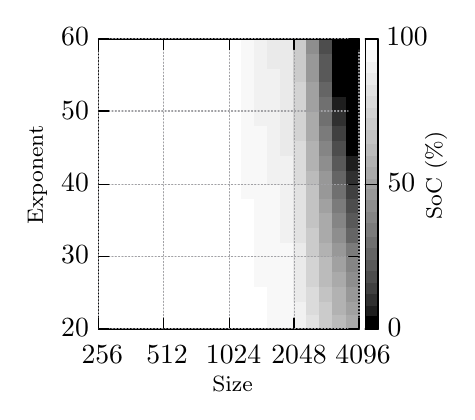
\begin{tikzpicture}[y=0.80pt, x=0.80pt, yscale=-0.600000, xscale=0.570000, inner sep=0pt, outer sep=0pt]
\begin{scope}[draw=black,line join=bevel,line cap=rect,even odd rule,line width=0.512pt]
  \begin{scope}[cm={{1.0,0.0,0.0,1.0,(0.0,0.0)}},draw=black,line join=bevel,line cap=rect,line width=0.512pt]
  \end{scope}
  \begin{scope}[cm={{1.00625,0.0,0.0,1.00625,(0.0,0.0)}},draw=black,line join=bevel,line cap=rect,line width=0.512pt]
  \end{scope}
  \begin{scope}[cm={{1.00625,0.0,0.0,1.00625,(0.0,0.0)}},draw=black,line join=bevel,line cap=rect,line width=0.512pt]
  \end{scope}
  \begin{scope}[cm={{1.00625,0.0,0.0,1.00625,(0.0,0.0)}},draw=black,line join=bevel,line cap=rect,line width=0.512pt]
  \end{scope}
  \begin{scope}[cm={{1.00625,0.0,0.0,1.00625,(0.0,0.0)}},draw=cffffff,fill=cffffff,line join=bevel,line cap=rect,line width=0.512pt]
    \path[draw,fill,even odd rule] (57.5000,268.5000) -- (57.5000,257.5000) --
      (67.5000,257.5000) -- (67.5000,268.5000) -- (57.5000,268.5000);
    \path[draw,fill,even odd rule] (67.5000,268.5000) -- (67.5000,257.5000) --
      (78.5000,257.5000) -- (78.5000,268.5000) -- (67.5000,268.5000);
    \path[draw,fill,even odd rule] (78.5000,268.5000) -- (78.5000,257.5000) --
      (88.5000,257.5000) -- (88.5000,268.5000) -- (78.5000,268.5000);
    \path[draw,fill,even odd rule] (88.5000,268.5000) -- (88.5000,257.5000) --
      (98.5000,257.5000) -- (98.5000,268.5000) -- (88.5000,268.5000);
    \path[draw,fill,even odd rule] (98.5000,268.5000) -- (98.5000,257.5000) --
      (108.5000,257.5000) -- (108.5000,268.5000) -- (98.5000,268.5000);
    \path[draw,fill,even odd rule] (57.5000,257.5000) -- (57.5000,247.5000) --
      (67.5000,247.5000) -- (67.5000,257.5000) -- (57.5000,257.5000);
    \path[draw,fill,even odd rule] (67.5000,257.5000) -- (67.5000,247.5000) --
      (78.5000,247.5000) -- (78.5000,257.5000) -- (67.5000,257.5000);
    \path[draw,fill,even odd rule] (78.5000,257.5000) -- (78.5000,247.5000) --
      (88.5000,247.5000) -- (88.5000,257.5000) -- (78.5000,257.5000);
    \path[draw,fill,even odd rule] (88.5000,257.5000) -- (88.5000,247.5000) --
      (98.5000,247.5000) -- (98.5000,257.5000) -- (88.5000,257.5000);
    \path[draw,fill,even odd rule] (98.5000,257.5000) -- (98.5000,247.5000) --
      (108.5000,247.5000) -- (108.5000,257.5000) -- (98.5000,257.5000);
    \path[draw,fill,even odd rule] (57.5000,247.5000) -- (57.5000,236.5000) --
      (67.5000,236.5000) -- (67.5000,247.5000) -- (57.5000,247.5000);
    \path[draw,fill,even odd rule] (67.5000,247.5000) -- (67.5000,236.5000) --
      (78.5000,236.5000) -- (78.5000,247.5000) -- (67.5000,247.5000);
    \path[draw,fill,even odd rule] (78.5000,247.5000) -- (78.5000,236.5000) --
      (88.5000,236.5000) -- (88.5000,247.5000) -- (78.5000,247.5000);
    \path[draw,fill,even odd rule] (88.5000,247.5000) -- (88.5000,236.5000) --
      (98.5000,236.5000) -- (98.5000,247.5000) -- (88.5000,247.5000);
    \path[draw,fill,even odd rule] (98.5000,247.5000) -- (98.5000,236.5000) --
      (108.5000,236.5000) -- (108.5000,247.5000) -- (98.5000,247.5000);
    \path[draw,fill,even odd rule] (57.5000,236.5000) -- (57.5000,225.5000) --
      (67.5000,225.5000) -- (67.5000,236.5000) -- (57.5000,236.5000);
    \path[draw,fill,even odd rule] (67.5000,236.5000) -- (67.5000,225.5000) --
      (78.5000,225.5000) -- (78.5000,236.5000) -- (67.5000,236.5000);
    \path[draw,fill,even odd rule] (78.5000,236.5000) -- (78.5000,225.5000) --
      (88.5000,225.5000) -- (88.5000,236.5000) -- (78.5000,236.5000);
    \path[draw,fill,even odd rule] (88.5000,236.5000) -- (88.5000,225.5000) --
      (98.5000,225.5000) -- (98.5000,236.5000) -- (88.5000,236.5000);
    \path[draw,fill,even odd rule] (98.5000,236.5000) -- (98.5000,225.5000) --
      (108.5000,225.5000) -- (108.5000,236.5000) -- (98.5000,236.5000);
    \path[draw,fill,even odd rule] (57.5000,225.5000) -- (57.5000,214.5000) --
      (67.5000,214.5000) -- (67.5000,225.5000) -- (57.5000,225.5000);
    \path[draw,fill,even odd rule] (67.5000,225.5000) -- (67.5000,214.5000) --
      (78.5000,214.5000) -- (78.5000,225.5000) -- (67.5000,225.5000);
    \path[draw,fill,even odd rule] (78.5000,225.5000) -- (78.5000,214.5000) --
      (88.5000,214.5000) -- (88.5000,225.5000) -- (78.5000,225.5000);
    \path[draw,fill,even odd rule] (88.5000,225.5000) -- (88.5000,214.5000) --
      (98.5000,214.5000) -- (98.5000,225.5000) -- (88.5000,225.5000);
    \path[draw,fill,even odd rule] (98.5000,225.5000) -- (98.5000,214.5000) --
      (108.5000,214.5000) -- (108.5000,225.5000) -- (98.5000,225.5000);
    \path[draw,fill,even odd rule] (57.5000,214.5000) -- (57.5000,203.5000) --
      (67.5000,203.5000) -- (67.5000,214.5000) -- (57.5000,214.5000);
    \path[draw,fill,even odd rule] (67.5000,214.5000) -- (67.5000,203.5000) --
      (78.5000,203.5000) -- (78.5000,214.5000) -- (67.5000,214.5000);
    \path[draw,fill,even odd rule] (78.5000,214.5000) -- (78.5000,203.5000) --
      (88.5000,203.5000) -- (88.5000,214.5000) -- (78.5000,214.5000);
    \path[draw,fill,even odd rule] (88.5000,214.5000) -- (88.5000,203.5000) --
      (98.5000,203.5000) -- (98.5000,214.5000) -- (88.5000,214.5000);
    \path[draw,fill,even odd rule] (98.5000,214.5000) -- (98.5000,203.5000) --
      (108.5000,203.5000) -- (108.5000,214.5000) -- (98.5000,214.5000);
    \path[draw,fill,even odd rule] (57.5000,203.5000) -- (57.5000,192.5000) --
      (67.5000,192.5000) -- (67.5000,203.5000) -- (57.5000,203.5000);
    \path[draw,fill,even odd rule] (67.5000,203.5000) -- (67.5000,192.5000) --
      (78.5000,192.5000) -- (78.5000,203.5000) -- (67.5000,203.5000);
    \path[draw,fill,even odd rule] (78.5000,203.5000) -- (78.5000,192.5000) --
      (88.5000,192.5000) -- (88.5000,203.5000) -- (78.5000,203.5000);
    \path[draw,fill,even odd rule] (88.5000,203.5000) -- (88.5000,192.5000) --
      (98.5000,192.5000) -- (98.5000,203.5000) -- (88.5000,203.5000);
    \path[draw,fill,even odd rule] (98.5000,203.5000) -- (98.5000,192.5000) --
      (108.5000,192.5000) -- (108.5000,203.5000) -- (98.5000,203.5000);
    \path[draw,fill,even odd rule] (57.5000,192.5000) -- (57.5000,181.5000) --
      (67.5000,181.5000) -- (67.5000,192.5000) -- (57.5000,192.5000);
    \path[draw,fill,even odd rule] (67.5000,192.5000) -- (67.5000,181.5000) --
      (78.5000,181.5000) -- (78.5000,192.5000) -- (67.5000,192.5000);
    \path[draw,fill,even odd rule] (78.5000,192.5000) -- (78.5000,181.5000) --
      (88.5000,181.5000) -- (88.5000,192.5000) -- (78.5000,192.5000);
    \path[draw,fill,even odd rule] (88.5000,192.5000) -- (88.5000,181.5000) --
      (98.5000,181.5000) -- (98.5000,192.5000) -- (88.5000,192.5000);
    \path[draw,fill,even odd rule] (98.5000,192.5000) -- (98.5000,181.5000) --
      (108.5000,181.5000) -- (108.5000,192.5000) -- (98.5000,192.5000);
    \path[draw,fill,even odd rule] (57.5000,181.5000) -- (57.5000,170.5000) --
      (67.5000,170.5000) -- (67.5000,181.5000) -- (57.5000,181.5000);
    \path[draw,fill,even odd rule] (67.5000,181.5000) -- (67.5000,170.5000) --
      (78.5000,170.5000) -- (78.5000,181.5000) -- (67.5000,181.5000);
    \path[draw,fill,even odd rule] (78.5000,181.5000) -- (78.5000,170.5000) --
      (88.5000,170.5000) -- (88.5000,181.5000) -- (78.5000,181.5000);
    \path[draw,fill,even odd rule] (88.5000,181.5000) -- (88.5000,170.5000) --
      (98.5000,170.5000) -- (98.5000,181.5000) -- (88.5000,181.5000);
    \path[draw,fill,even odd rule] (98.5000,181.5000) -- (98.5000,170.5000) --
      (108.5000,170.5000) -- (108.5000,181.5000) -- (98.5000,181.5000);
    \path[draw,fill,even odd rule] (57.5000,170.5000) -- (57.5000,160.5000) --
      (67.5000,160.5000) -- (67.5000,170.5000) -- (57.5000,170.5000);
    \path[draw,fill,even odd rule] (67.5000,170.5000) -- (67.5000,160.5000) --
      (78.5000,160.5000) -- (78.5000,170.5000) -- (67.5000,170.5000);
    \path[draw,fill,even odd rule] (78.5000,170.5000) -- (78.5000,160.5000) --
      (88.5000,160.5000) -- (88.5000,170.5000) -- (78.5000,170.5000);
    \path[draw,fill,even odd rule] (88.5000,170.5000) -- (88.5000,160.5000) --
      (98.5000,160.5000) -- (98.5000,170.5000) -- (88.5000,170.5000);
    \path[draw,fill,even odd rule] (98.5000,170.5000) -- (98.5000,160.5000) --
      (108.5000,160.5000) -- (108.5000,170.5000) -- (98.5000,170.5000);
    \path[draw,fill,even odd rule] (57.5000,160.5000) -- (57.5000,149.5000) --
      (67.5000,149.5000) -- (67.5000,160.5000) -- (57.5000,160.5000);
    \path[draw,fill,even odd rule] (67.5000,160.5000) -- (67.5000,149.5000) --
      (78.5000,149.5000) -- (78.5000,160.5000) -- (67.5000,160.5000);
    \path[draw,fill,even odd rule] (78.5000,160.5000) -- (78.5000,149.5000) --
      (88.5000,149.5000) -- (88.5000,160.5000) -- (78.5000,160.5000);
    \path[draw,fill,even odd rule] (88.5000,160.5000) -- (88.5000,149.5000) --
      (98.5000,149.5000) -- (98.5000,160.5000) -- (88.5000,160.5000);
    \path[draw,fill,even odd rule] (98.5000,160.5000) -- (98.5000,149.5000) --
      (108.5000,149.5000) -- (108.5000,160.5000) -- (98.5000,160.5000);
    \path[draw,fill,even odd rule] (57.5000,149.5000) -- (57.5000,138.5000) --
      (67.5000,138.5000) -- (67.5000,149.5000) -- (57.5000,149.5000);
    \path[draw,fill,even odd rule] (67.5000,149.5000) -- (67.5000,138.5000) --
      (78.5000,138.5000) -- (78.5000,149.5000) -- (67.5000,149.5000);
    \path[draw,fill,even odd rule] (78.5000,149.5000) -- (78.5000,138.5000) --
      (88.5000,138.5000) -- (88.5000,149.5000) -- (78.5000,149.5000);
    \path[draw,fill,even odd rule] (88.5000,149.5000) -- (88.5000,138.5000) --
      (98.5000,138.5000) -- (98.5000,149.5000) -- (88.5000,149.5000);
    \path[draw,fill,even odd rule] (98.5000,149.5000) -- (98.5000,138.5000) --
      (108.5000,138.5000) -- (108.5000,149.5000) -- (98.5000,149.5000);
    \path[draw,fill,even odd rule] (57.5000,138.5000) -- (57.5000,127.5000) --
      (67.5000,127.5000) -- (67.5000,138.5000) -- (57.5000,138.5000);
    \path[draw,fill,even odd rule] (67.5000,138.5000) -- (67.5000,127.5000) --
      (78.5000,127.5000) -- (78.5000,138.5000) -- (67.5000,138.5000);
    \path[draw,fill,even odd rule] (78.5000,138.5000) -- (78.5000,127.5000) --
      (88.5000,127.5000) -- (88.5000,138.5000) -- (78.5000,138.5000);
    \path[draw,fill,even odd rule] (88.5000,138.5000) -- (88.5000,127.5000) --
      (98.5000,127.5000) -- (98.5000,138.5000) -- (88.5000,138.5000);
    \path[draw,fill,even odd rule] (98.5000,138.5000) -- (98.5000,127.5000) --
      (108.5000,127.5000) -- (108.5000,138.5000) -- (98.5000,138.5000);
    \path[draw,fill,even odd rule] (57.5000,127.5000) -- (57.5000,116.5000) --
      (67.5000,116.5000) -- (67.5000,127.5000) -- (57.5000,127.5000);
    \path[draw,fill,even odd rule] (67.5000,127.5000) -- (67.5000,116.5000) --
      (78.5000,116.5000) -- (78.5000,127.5000) -- (67.5000,127.5000);
    \path[draw,fill,even odd rule] (78.5000,127.5000) -- (78.5000,116.5000) --
      (88.5000,116.5000) -- (88.5000,127.5000) -- (78.5000,127.5000);
    \path[draw,fill,even odd rule] (88.5000,127.5000) -- (88.5000,116.5000) --
      (98.5000,116.5000) -- (98.5000,127.5000) -- (88.5000,127.5000);
    \path[draw,fill,even odd rule] (98.5000,127.5000) -- (98.5000,116.5000) --
      (108.5000,116.5000) -- (108.5000,127.5000) -- (98.5000,127.5000);
    \path[draw,fill,even odd rule] (57.5000,116.5000) -- (57.5000,105.5000) --
      (67.5000,105.5000) -- (67.5000,116.5000) -- (57.5000,116.5000);
    \path[draw,fill,even odd rule] (67.5000,116.5000) -- (67.5000,105.5000) --
      (78.5000,105.5000) -- (78.5000,116.5000) -- (67.5000,116.5000);
    \path[draw,fill,even odd rule] (78.5000,116.5000) -- (78.5000,105.5000) --
      (88.5000,105.5000) -- (88.5000,116.5000) -- (78.5000,116.5000);
    \path[draw,fill,even odd rule] (88.5000,116.5000) -- (88.5000,105.5000) --
      (98.5000,105.5000) -- (98.5000,116.5000) -- (88.5000,116.5000);
    \path[draw,fill,even odd rule] (98.5000,116.5000) -- (98.5000,105.5000) --
      (108.5000,105.5000) -- (108.5000,116.5000) -- (98.5000,116.5000);
    \path[draw,fill,even odd rule] (57.5000,105.5000) -- (57.5000,94.5000) --
      (67.5000,94.5000) -- (67.5000,105.5000) -- (57.5000,105.5000);
    \path[draw,fill,even odd rule] (67.5000,105.5000) -- (67.5000,94.5000) --
      (78.5000,94.5000) -- (78.5000,105.5000) -- (67.5000,105.5000);
    \path[draw,fill,even odd rule] (78.5000,105.5000) -- (78.5000,94.5000) --
      (88.5000,94.5000) -- (88.5000,105.5000) -- (78.5000,105.5000);
    \path[draw,fill,even odd rule] (88.5000,105.5000) -- (88.5000,94.5000) --
      (98.5000,94.5000) -- (98.5000,105.5000) -- (88.5000,105.5000);
    \path[draw,fill,even odd rule] (98.5000,105.5000) -- (98.5000,94.5000) --
      (108.5000,94.5000) -- (108.5000,105.5000) -- (98.5000,105.5000);
    \path[draw,fill,even odd rule] (57.5000,94.5000) -- (57.5000,83.5000) --
      (67.5000,83.5000) -- (67.5000,94.5000) -- (57.5000,94.5000);
    \path[draw,fill,even odd rule] (67.5000,94.5000) -- (67.5000,83.5000) --
      (78.5000,83.5000) -- (78.5000,94.5000) -- (67.5000,94.5000);
    \path[draw,fill,even odd rule] (78.5000,94.5000) -- (78.5000,83.5000) --
      (88.5000,83.5000) -- (88.5000,94.5000) -- (78.5000,94.5000);
    \path[draw,fill,even odd rule] (88.5000,94.5000) -- (88.5000,83.5000) --
      (98.5000,83.5000) -- (98.5000,94.5000) -- (88.5000,94.5000);
    \path[draw,fill,even odd rule] (98.5000,94.5000) -- (98.5000,83.5000) --
      (108.5000,83.5000) -- (108.5000,94.5000) -- (98.5000,94.5000);
    \path[draw,fill,even odd rule] (57.5000,83.5000) -- (57.5000,73.5000) --
      (67.5000,73.5000) -- (67.5000,83.5000) -- (57.5000,83.5000);
    \path[draw,fill,even odd rule] (67.5000,83.5000) -- (67.5000,73.5000) --
      (78.5000,73.5000) -- (78.5000,83.5000) -- (67.5000,83.5000);
    \path[draw,fill,even odd rule] (78.5000,83.5000) -- (78.5000,73.5000) --
      (88.5000,73.5000) -- (88.5000,83.5000) -- (78.5000,83.5000);
    \path[draw,fill,even odd rule] (88.5000,83.5000) -- (88.5000,73.5000) --
      (98.5000,73.5000) -- (98.5000,83.5000) -- (88.5000,83.5000);
    \path[draw,fill,even odd rule] (98.5000,83.5000) -- (98.5000,73.5000) --
      (108.5000,73.5000) -- (108.5000,83.5000) -- (98.5000,83.5000);
    \path[draw,fill,even odd rule] (57.5000,73.5000) -- (57.5000,62.5000) --
      (67.5000,62.5000) -- (67.5000,73.5000) -- (57.5000,73.5000);
    \path[draw,fill,even odd rule] (67.5000,73.5000) -- (67.5000,62.5000) --
      (78.5000,62.5000) -- (78.5000,73.5000) -- (67.5000,73.5000);
    \path[draw,fill,even odd rule] (78.5000,73.5000) -- (78.5000,62.5000) --
      (88.5000,62.5000) -- (88.5000,73.5000) -- (78.5000,73.5000);
    \path[draw,fill,even odd rule] (88.5000,73.5000) -- (88.5000,62.5000) --
      (98.5000,62.5000) -- (98.5000,73.5000) -- (88.5000,73.5000);
    \path[draw,fill,even odd rule] (98.5000,73.5000) -- (98.5000,62.5000) --
      (108.5000,62.5000) -- (108.5000,73.5000) -- (98.5000,73.5000);
    \path[draw,fill,even odd rule] (57.5000,62.5000) -- (57.5000,51.5000) --
      (67.5000,51.5000) -- (67.5000,62.5000) -- (57.5000,62.5000);
    \path[draw,fill,even odd rule] (67.5000,62.5000) -- (67.5000,51.5000) --
      (78.5000,51.5000) -- (78.5000,62.5000) -- (67.5000,62.5000);
    \path[draw,fill,even odd rule] (78.5000,62.5000) -- (78.5000,51.5000) --
      (88.5000,51.5000) -- (88.5000,62.5000) -- (78.5000,62.5000);
    \path[draw,fill,even odd rule] (88.5000,62.5000) -- (88.5000,51.5000) --
      (98.5000,51.5000) -- (98.5000,62.5000) -- (88.5000,62.5000);
    \path[draw,fill,even odd rule] (98.5000,62.5000) -- (98.5000,51.5000) --
      (108.5000,51.5000) -- (108.5000,62.5000) -- (98.5000,62.5000);
    \path[draw,fill,even odd rule] (108.5000,268.5000) -- (108.5000,257.5000) --
      (119.5000,257.5000) -- (119.5000,268.5000) -- (108.5000,268.5000);
    \path[draw,fill,even odd rule] (119.5000,268.5000) -- (119.5000,257.5000) --
      (129.5000,257.5000) -- (129.5000,268.5000) -- (119.5000,268.5000);
    \path[draw,fill,even odd rule] (129.5000,268.5000) -- (129.5000,257.5000) --
      (139.5000,257.5000) -- (139.5000,268.5000) -- (129.5000,268.5000);
    \path[draw,fill,even odd rule] (139.5000,268.5000) -- (139.5000,257.5000) --
      (149.5000,257.5000) -- (149.5000,268.5000) -- (139.5000,268.5000);
    \path[draw,fill,even odd rule] (149.5000,268.5000) -- (149.5000,257.5000) --
      (160.5000,257.5000) -- (160.5000,268.5000) -- (149.5000,268.5000);
    \path[draw,fill,even odd rule] (108.5000,257.5000) -- (108.5000,247.5000) --
      (119.5000,247.5000) -- (119.5000,257.5000) -- (108.5000,257.5000);
    \path[draw,fill,even odd rule] (119.5000,257.5000) -- (119.5000,247.5000) --
      (129.5000,247.5000) -- (129.5000,257.5000) -- (119.5000,257.5000);
    \path[draw,fill,even odd rule] (129.5000,257.5000) -- (129.5000,247.5000) --
      (139.5000,247.5000) -- (139.5000,257.5000) -- (129.5000,257.5000);
    \path[draw,fill,even odd rule] (139.5000,257.5000) -- (139.5000,247.5000) --
      (149.5000,247.5000) -- (149.5000,257.5000) -- (139.5000,257.5000);
    \path[draw,fill,even odd rule] (149.5000,257.5000) -- (149.5000,247.5000) --
      (160.5000,247.5000) -- (160.5000,257.5000) -- (149.5000,257.5000);
    \path[draw,fill,even odd rule] (108.5000,247.5000) -- (108.5000,236.5000) --
      (119.5000,236.5000) -- (119.5000,247.5000) -- (108.5000,247.5000);
    \path[draw,fill,even odd rule] (119.5000,247.5000) -- (119.5000,236.5000) --
      (129.5000,236.5000) -- (129.5000,247.5000) -- (119.5000,247.5000);
    \path[draw,fill,even odd rule] (129.5000,247.5000) -- (129.5000,236.5000) --
      (139.5000,236.5000) -- (139.5000,247.5000) -- (129.5000,247.5000);
    \path[draw,fill,even odd rule] (139.5000,247.5000) -- (139.5000,236.5000) --
      (149.5000,236.5000) -- (149.5000,247.5000) -- (139.5000,247.5000);
    \path[draw,fill,even odd rule] (149.5000,247.5000) -- (149.5000,236.5000) --
      (160.5000,236.5000) -- (160.5000,247.5000) -- (149.5000,247.5000);
    \path[draw,fill,even odd rule] (108.5000,236.5000) -- (108.5000,225.5000) --
      (119.5000,225.5000) -- (119.5000,236.5000) -- (108.5000,236.5000);
    \path[draw,fill,even odd rule] (119.5000,236.5000) -- (119.5000,225.5000) --
      (129.5000,225.5000) -- (129.5000,236.5000) -- (119.5000,236.5000);
    \path[draw,fill,even odd rule] (129.5000,236.5000) -- (129.5000,225.5000) --
      (139.5000,225.5000) -- (139.5000,236.5000) -- (129.5000,236.5000);
    \path[draw,fill,even odd rule] (139.5000,236.5000) -- (139.5000,225.5000) --
      (149.5000,225.5000) -- (149.5000,236.5000) -- (139.5000,236.5000);
    \path[draw,fill,even odd rule] (149.5000,236.5000) -- (149.5000,225.5000) --
      (160.5000,225.5000) -- (160.5000,236.5000) -- (149.5000,236.5000);
    \path[draw,fill,even odd rule] (108.5000,225.5000) -- (108.5000,214.5000) --
      (119.5000,214.5000) -- (119.5000,225.5000) -- (108.5000,225.5000);
    \path[draw,fill,even odd rule] (119.5000,225.5000) -- (119.5000,214.5000) --
      (129.5000,214.5000) -- (129.5000,225.5000) -- (119.5000,225.5000);
    \path[draw,fill,even odd rule] (129.5000,225.5000) -- (129.5000,214.5000) --
      (139.5000,214.5000) -- (139.5000,225.5000) -- (129.5000,225.5000);
    \path[draw,fill,even odd rule] (139.5000,225.5000) -- (139.5000,214.5000) --
      (149.5000,214.5000) -- (149.5000,225.5000) -- (139.5000,225.5000);
    \path[draw,fill,even odd rule] (149.5000,225.5000) -- (149.5000,214.5000) --
      (160.5000,214.5000) -- (160.5000,225.5000) -- (149.5000,225.5000);
    \path[draw,fill,even odd rule] (108.5000,214.5000) -- (108.5000,203.5000) --
      (119.5000,203.5000) -- (119.5000,214.5000) -- (108.5000,214.5000);
    \path[draw,fill,even odd rule] (119.5000,214.5000) -- (119.5000,203.5000) --
      (129.5000,203.5000) -- (129.5000,214.5000) -- (119.5000,214.5000);
    \path[draw,fill,even odd rule] (129.5000,214.5000) -- (129.5000,203.5000) --
      (139.5000,203.5000) -- (139.5000,214.5000) -- (129.5000,214.5000);
    \path[draw,fill,even odd rule] (139.5000,214.5000) -- (139.5000,203.5000) --
      (149.5000,203.5000) -- (149.5000,214.5000) -- (139.5000,214.5000);
    \path[draw,fill,even odd rule] (149.5000,214.5000) -- (149.5000,203.5000) --
      (160.5000,203.5000) -- (160.5000,214.5000) -- (149.5000,214.5000);
    \path[draw,fill,even odd rule] (108.5000,203.5000) -- (108.5000,192.5000) --
      (119.5000,192.5000) -- (119.5000,203.5000) -- (108.5000,203.5000);
    \path[draw,fill,even odd rule] (119.5000,203.5000) -- (119.5000,192.5000) --
      (129.5000,192.5000) -- (129.5000,203.5000) -- (119.5000,203.5000);
    \path[draw,fill,even odd rule] (129.5000,203.5000) -- (129.5000,192.5000) --
      (139.5000,192.5000) -- (139.5000,203.5000) -- (129.5000,203.5000);
    \path[draw,fill,even odd rule] (139.5000,203.5000) -- (139.5000,192.5000) --
      (149.5000,192.5000) -- (149.5000,203.5000) -- (139.5000,203.5000);
    \path[draw,fill,even odd rule] (149.5000,203.5000) -- (149.5000,192.5000) --
      (160.5000,192.5000) -- (160.5000,203.5000) -- (149.5000,203.5000);
    \path[draw,fill,even odd rule] (108.5000,192.5000) -- (108.5000,181.5000) --
      (119.5000,181.5000) -- (119.5000,192.5000) -- (108.5000,192.5000);
    \path[draw,fill,even odd rule] (119.5000,192.5000) -- (119.5000,181.5000) --
      (129.5000,181.5000) -- (129.5000,192.5000) -- (119.5000,192.5000);
    \path[draw,fill,even odd rule] (129.5000,192.5000) -- (129.5000,181.5000) --
      (139.5000,181.5000) -- (139.5000,192.5000) -- (129.5000,192.5000);
    \path[draw,fill,even odd rule] (139.5000,192.5000) -- (139.5000,181.5000) --
      (149.5000,181.5000) -- (149.5000,192.5000) -- (139.5000,192.5000);
    \path[draw,fill,even odd rule] (149.5000,192.5000) -- (149.5000,181.5000) --
      (160.5000,181.5000) -- (160.5000,192.5000) -- (149.5000,192.5000);
    \path[draw,fill,even odd rule] (108.5000,181.5000) -- (108.5000,170.5000) --
      (119.5000,170.5000) -- (119.5000,181.5000) -- (108.5000,181.5000);
    \path[draw,fill,even odd rule] (119.5000,181.5000) -- (119.5000,170.5000) --
      (129.5000,170.5000) -- (129.5000,181.5000) -- (119.5000,181.5000);
    \path[draw,fill,even odd rule] (129.5000,181.5000) -- (129.5000,170.5000) --
      (139.5000,170.5000) -- (139.5000,181.5000) -- (129.5000,181.5000);
    \path[draw,fill,even odd rule] (139.5000,181.5000) -- (139.5000,170.5000) --
      (149.5000,170.5000) -- (149.5000,181.5000) -- (139.5000,181.5000);
    \path[draw,fill,even odd rule] (149.5000,181.5000) -- (149.5000,170.5000) --
      (160.5000,170.5000) -- (160.5000,181.5000) -- (149.5000,181.5000);
    \path[draw,fill,even odd rule] (108.5000,170.5000) -- (108.5000,160.5000) --
      (119.5000,160.5000) -- (119.5000,170.5000) -- (108.5000,170.5000);
    \path[draw,fill,even odd rule] (119.5000,170.5000) -- (119.5000,160.5000) --
      (129.5000,160.5000) -- (129.5000,170.5000) -- (119.5000,170.5000);
    \path[draw,fill,even odd rule] (129.5000,170.5000) -- (129.5000,160.5000) --
      (139.5000,160.5000) -- (139.5000,170.5000) -- (129.5000,170.5000);
    \path[draw,fill,even odd rule] (139.5000,170.5000) -- (139.5000,160.5000) --
      (149.5000,160.5000) -- (149.5000,170.5000) -- (139.5000,170.5000);
    \path[draw,fill,even odd rule] (149.5000,170.5000) -- (149.5000,160.5000) --
      (160.5000,160.5000) -- (160.5000,170.5000) -- (149.5000,170.5000);
    \path[draw,fill,even odd rule] (108.5000,160.5000) -- (108.5000,149.5000) --
      (119.5000,149.5000) -- (119.5000,160.5000) -- (108.5000,160.5000);
    \path[draw,fill,even odd rule] (119.5000,160.5000) -- (119.5000,149.5000) --
      (129.5000,149.5000) -- (129.5000,160.5000) -- (119.5000,160.5000);
    \path[draw,fill,even odd rule] (129.5000,160.5000) -- (129.5000,149.5000) --
      (139.5000,149.5000) -- (139.5000,160.5000) -- (129.5000,160.5000);
    \path[draw,fill,even odd rule] (139.5000,160.5000) -- (139.5000,149.5000) --
      (149.5000,149.5000) -- (149.5000,160.5000) -- (139.5000,160.5000);
    \path[draw,fill,even odd rule] (149.5000,160.5000) -- (149.5000,149.5000) --
      (160.5000,149.5000) -- (160.5000,160.5000) -- (149.5000,160.5000);
    \path[draw,fill,even odd rule] (108.5000,149.5000) -- (108.5000,138.5000) --
      (119.5000,138.5000) -- (119.5000,149.5000) -- (108.5000,149.5000);
    \path[draw,fill,even odd rule] (119.5000,149.5000) -- (119.5000,138.5000) --
      (129.5000,138.5000) -- (129.5000,149.5000) -- (119.5000,149.5000);
    \path[draw,fill,even odd rule] (129.5000,149.5000) -- (129.5000,138.5000) --
      (139.5000,138.5000) -- (139.5000,149.5000) -- (129.5000,149.5000);
    \path[draw,fill,even odd rule] (139.5000,149.5000) -- (139.5000,138.5000) --
      (149.5000,138.5000) -- (149.5000,149.5000) -- (139.5000,149.5000);
    \path[draw,fill,even odd rule] (149.5000,149.5000) -- (149.5000,138.5000) --
      (160.5000,138.5000) -- (160.5000,149.5000) -- (149.5000,149.5000);
    \path[draw,fill,even odd rule] (108.5000,138.5000) -- (108.5000,127.5000) --
      (119.5000,127.5000) -- (119.5000,138.5000) -- (108.5000,138.5000);
    \path[draw,fill,even odd rule] (119.5000,138.5000) -- (119.5000,127.5000) --
      (129.5000,127.5000) -- (129.5000,138.5000) -- (119.5000,138.5000);
    \path[draw,fill,even odd rule] (129.5000,138.5000) -- (129.5000,127.5000) --
      (139.5000,127.5000) -- (139.5000,138.5000) -- (129.5000,138.5000);
    \path[draw,fill,even odd rule] (139.5000,138.5000) -- (139.5000,127.5000) --
      (149.5000,127.5000) -- (149.5000,138.5000) -- (139.5000,138.5000);
    \path[draw,fill,even odd rule] (149.5000,138.5000) -- (149.5000,127.5000) --
      (160.5000,127.5000) -- (160.5000,138.5000) -- (149.5000,138.5000);
    \path[draw,fill,even odd rule] (108.5000,127.5000) -- (108.5000,116.5000) --
      (119.5000,116.5000) -- (119.5000,127.5000) -- (108.5000,127.5000);
    \path[draw,fill,even odd rule] (119.5000,127.5000) -- (119.5000,116.5000) --
      (129.5000,116.5000) -- (129.5000,127.5000) -- (119.5000,127.5000);
    \path[draw,fill,even odd rule] (129.5000,127.5000) -- (129.5000,116.5000) --
      (139.5000,116.5000) -- (139.5000,127.5000) -- (129.5000,127.5000);
    \path[draw,fill,even odd rule] (139.5000,127.5000) -- (139.5000,116.5000) --
      (149.5000,116.5000) -- (149.5000,127.5000) -- (139.5000,127.5000);
    \path[draw,fill,even odd rule] (149.5000,127.5000) -- (149.5000,116.5000) --
      (160.5000,116.5000) -- (160.5000,127.5000) -- (149.5000,127.5000);
    \path[draw,fill,even odd rule] (108.5000,116.5000) -- (108.5000,105.5000) --
      (119.5000,105.5000) -- (119.5000,116.5000) -- (108.5000,116.5000);
    \path[draw,fill,even odd rule] (119.5000,116.5000) -- (119.5000,105.5000) --
      (129.5000,105.5000) -- (129.5000,116.5000) -- (119.5000,116.5000);
    \path[draw,fill,even odd rule] (129.5000,116.5000) -- (129.5000,105.5000) --
      (139.5000,105.5000) -- (139.5000,116.5000) -- (129.5000,116.5000);
    \path[draw,fill,even odd rule] (139.5000,116.5000) -- (139.5000,105.5000) --
      (149.5000,105.5000) -- (149.5000,116.5000) -- (139.5000,116.5000);
    \path[draw,fill,even odd rule] (149.5000,116.5000) -- (149.5000,105.5000) --
      (160.5000,105.5000) -- (160.5000,116.5000) -- (149.5000,116.5000);
    \path[draw,fill,even odd rule] (108.5000,105.5000) -- (108.5000,94.5000) --
      (119.5000,94.5000) -- (119.5000,105.5000) -- (108.5000,105.5000);
    \path[draw,fill,even odd rule] (119.5000,105.5000) -- (119.5000,94.5000) --
      (129.5000,94.5000) -- (129.5000,105.5000) -- (119.5000,105.5000);
    \path[draw,fill,even odd rule] (129.5000,105.5000) -- (129.5000,94.5000) --
      (139.5000,94.5000) -- (139.5000,105.5000) -- (129.5000,105.5000);
    \path[draw,fill,even odd rule] (139.5000,105.5000) -- (139.5000,94.5000) --
      (149.5000,94.5000) -- (149.5000,105.5000) -- (139.5000,105.5000);
    \path[draw,fill,even odd rule] (149.5000,105.5000) -- (149.5000,94.5000) --
      (160.5000,94.5000) -- (160.5000,105.5000) -- (149.5000,105.5000);
    \path[draw,fill,even odd rule] (108.5000,94.5000) -- (108.5000,83.5000) --
      (119.5000,83.5000) -- (119.5000,94.5000) -- (108.5000,94.5000);
    \path[draw,fill,even odd rule] (119.5000,94.5000) -- (119.5000,83.5000) --
      (129.5000,83.5000) -- (129.5000,94.5000) -- (119.5000,94.5000);
    \path[draw,fill,even odd rule] (129.5000,94.5000) -- (129.5000,83.5000) --
      (139.5000,83.5000) -- (139.5000,94.5000) -- (129.5000,94.5000);
    \path[draw,fill,even odd rule] (139.5000,94.5000) -- (139.5000,83.5000) --
      (149.5000,83.5000) -- (149.5000,94.5000) -- (139.5000,94.5000);
    \path[draw,fill,even odd rule] (149.5000,94.5000) -- (149.5000,83.5000) --
      (160.5000,83.5000) -- (160.5000,94.5000) -- (149.5000,94.5000);
    \path[draw,fill,even odd rule] (108.5000,83.5000) -- (108.5000,73.5000) --
      (119.5000,73.5000) -- (119.5000,83.5000) -- (108.5000,83.5000);
    \path[draw,fill,even odd rule] (119.5000,83.5000) -- (119.5000,73.5000) --
      (129.5000,73.5000) -- (129.5000,83.5000) -- (119.5000,83.5000);
    \path[draw,fill,even odd rule] (129.5000,83.5000) -- (129.5000,73.5000) --
      (139.5000,73.5000) -- (139.5000,83.5000) -- (129.5000,83.5000);
    \path[draw,fill,even odd rule] (139.5000,83.5000) -- (139.5000,73.5000) --
      (149.5000,73.5000) -- (149.5000,83.5000) -- (139.5000,83.5000);
    \path[draw,fill,even odd rule] (149.5000,83.5000) -- (149.5000,73.5000) --
      (160.5000,73.5000) -- (160.5000,83.5000) -- (149.5000,83.5000);
    \path[draw,fill,even odd rule] (108.5000,73.5000) -- (108.5000,62.5000) --
      (119.5000,62.5000) -- (119.5000,73.5000) -- (108.5000,73.5000);
    \path[draw,fill,even odd rule] (119.5000,73.5000) -- (119.5000,62.5000) --
      (129.5000,62.5000) -- (129.5000,73.5000) -- (119.5000,73.5000);
    \path[draw,fill,even odd rule] (129.5000,73.5000) -- (129.5000,62.5000) --
      (139.5000,62.5000) -- (139.5000,73.5000) -- (129.5000,73.5000);
    \path[draw,fill,even odd rule] (139.5000,73.5000) -- (139.5000,62.5000) --
      (149.5000,62.5000) -- (149.5000,73.5000) -- (139.5000,73.5000);
    \path[draw,fill,even odd rule] (149.5000,73.5000) -- (149.5000,62.5000) --
      (160.5000,62.5000) -- (160.5000,73.5000) -- (149.5000,73.5000);
    \path[draw,fill,even odd rule] (108.5000,62.5000) -- (108.5000,51.5000) --
      (119.5000,51.5000) -- (119.5000,62.5000) -- (108.5000,62.5000);
    \path[draw,fill,even odd rule] (119.5000,62.5000) -- (119.5000,51.5000) --
      (129.5000,51.5000) -- (129.5000,62.5000) -- (119.5000,62.5000);
    \path[draw,fill,even odd rule] (129.5000,62.5000) -- (129.5000,51.5000) --
      (139.5000,51.5000) -- (139.5000,62.5000) -- (129.5000,62.5000);
    \path[draw,fill,even odd rule] (139.5000,62.5000) -- (139.5000,51.5000) --
      (149.5000,51.5000) -- (149.5000,62.5000) -- (139.5000,62.5000);
    \path[draw,fill,even odd rule] (149.5000,62.5000) -- (149.5000,51.5000) --
      (160.5000,51.5000) -- (160.5000,62.5000) -- (149.5000,62.5000);
    \path[draw,fill,even odd rule] (160.5000,268.5000) -- (160.5000,257.5000) --
      (170.5000,257.5000) -- (170.5000,268.5000) -- (160.5000,268.5000);
    \path[draw,fill,even odd rule] (170.5000,268.5000) -- (170.5000,257.5000) --
      (180.5000,257.5000) -- (180.5000,268.5000) -- (170.5000,268.5000);
    \path[draw,fill,even odd rule] (180.5000,268.5000) -- (180.5000,257.5000) --
      (190.5000,257.5000) -- (190.5000,268.5000) -- (180.5000,268.5000);
  \end{scope}
  \begin{scope}[cm={{1.00625,0.0,0.0,1.00625,(0.0,0.0)}},draw=cf8f8f8,fill=cf8f8f8,line join=bevel,line cap=rect,line width=0.512pt]
    \path[draw,fill,even odd rule] (190.5000,268.5000) -- (190.5000,257.5000) --
      (200.5000,257.5000) -- (200.5000,268.5000) -- (190.5000,268.5000);
    \path[draw,fill,even odd rule] (200.5000,268.5000) -- (200.5000,257.5000) --
      (211.5000,257.5000) -- (211.5000,268.5000) -- (200.5000,268.5000);
  \end{scope}
  \begin{scope}[cm={{1.00625,0.0,0.0,1.00625,(0.0,0.0)}},draw=cffffff,fill=cffffff,line join=bevel,line cap=rect,line width=0.512pt]
    \path[draw,fill,even odd rule] (160.5000,257.5000) -- (160.5000,247.5000) --
      (170.5000,247.5000) -- (170.5000,257.5000) -- (160.5000,257.5000);
    \path[draw,fill,even odd rule] (170.5000,257.5000) -- (170.5000,247.5000) --
      (180.5000,247.5000) -- (180.5000,257.5000) -- (170.5000,257.5000);
    \path[draw,fill,even odd rule] (180.5000,257.5000) -- (180.5000,247.5000) --
      (190.5000,247.5000) -- (190.5000,257.5000) -- (180.5000,257.5000);
  \end{scope}
  \begin{scope}[cm={{1.00625,0.0,0.0,1.00625,(0.0,0.0)}},draw=cf8f8f8,fill=cf8f8f8,line join=bevel,line cap=rect,line width=0.512pt]
    \path[draw,fill,even odd rule] (190.5000,257.5000) -- (190.5000,247.5000) --
      (200.5000,247.5000) -- (200.5000,257.5000) -- (190.5000,257.5000);
    \path[draw,fill,even odd rule] (200.5000,257.5000) -- (200.5000,247.5000) --
      (211.5000,247.5000) -- (211.5000,257.5000) -- (200.5000,257.5000);
  \end{scope}
  \begin{scope}[cm={{1.00625,0.0,0.0,1.00625,(0.0,0.0)}},draw=cffffff,fill=cffffff,line join=bevel,line cap=rect,line width=0.512pt]
    \path[draw,fill,even odd rule] (160.5000,247.5000) -- (160.5000,236.5000) --
      (170.5000,236.5000) -- (170.5000,247.5000) -- (160.5000,247.5000);
    \path[draw,fill,even odd rule] (170.5000,247.5000) -- (170.5000,236.5000) --
      (180.5000,236.5000) -- (180.5000,247.5000) -- (170.5000,247.5000);
    \path[draw,fill,even odd rule] (180.5000,247.5000) -- (180.5000,236.5000) --
      (190.5000,236.5000) -- (190.5000,247.5000) -- (180.5000,247.5000);
  \end{scope}
  \begin{scope}[cm={{1.00625,0.0,0.0,1.00625,(0.0,0.0)}},draw=cf8f8f8,fill=cf8f8f8,line join=bevel,line cap=rect,line width=0.512pt]
    \path[draw,fill,even odd rule] (190.5000,247.5000) -- (190.5000,236.5000) --
      (200.5000,236.5000) -- (200.5000,247.5000) -- (190.5000,247.5000);
    \path[draw,fill,even odd rule] (200.5000,247.5000) -- (200.5000,236.5000) --
      (211.5000,236.5000) -- (211.5000,247.5000) -- (200.5000,247.5000);
  \end{scope}
  \begin{scope}[cm={{1.00625,0.0,0.0,1.00625,(0.0,0.0)}},draw=cffffff,fill=cffffff,line join=bevel,line cap=rect,line width=0.512pt]
    \path[draw,fill,even odd rule] (160.5000,236.5000) -- (160.5000,225.5000) --
      (170.5000,225.5000) -- (170.5000,236.5000) -- (160.5000,236.5000);
    \path[draw,fill,even odd rule] (170.5000,236.5000) -- (170.5000,225.5000) --
      (180.5000,225.5000) -- (180.5000,236.5000) -- (170.5000,236.5000);
  \end{scope}
  \begin{scope}[cm={{1.00625,0.0,0.0,1.00625,(0.0,0.0)}},draw=cf8f8f8,fill=cf8f8f8,line join=bevel,line cap=rect,line width=0.512pt]
    \path[draw,fill,even odd rule] (180.5000,236.5000) -- (180.5000,225.5000) --
      (190.5000,225.5000) -- (190.5000,236.5000) -- (180.5000,236.5000);
    \path[draw,fill,even odd rule] (190.5000,236.5000) -- (190.5000,225.5000) --
      (200.5000,225.5000) -- (200.5000,236.5000) -- (190.5000,236.5000);
    \path[draw,fill,even odd rule] (200.5000,236.5000) -- (200.5000,225.5000) --
      (211.5000,225.5000) -- (211.5000,236.5000) -- (200.5000,236.5000);
  \end{scope}
  \begin{scope}[cm={{1.00625,0.0,0.0,1.00625,(0.0,0.0)}},draw=cffffff,fill=cffffff,line join=bevel,line cap=rect,line width=0.512pt]
    \path[draw,fill,even odd rule] (160.5000,225.5000) -- (160.5000,214.5000) --
      (170.5000,214.5000) -- (170.5000,225.5000) -- (160.5000,225.5000);
    \path[draw,fill,even odd rule] (170.5000,225.5000) -- (170.5000,214.5000) --
      (180.5000,214.5000) -- (180.5000,225.5000) -- (170.5000,225.5000);
  \end{scope}
  \begin{scope}[cm={{1.00625,0.0,0.0,1.00625,(0.0,0.0)}},draw=cf8f8f8,fill=cf8f8f8,line join=bevel,line cap=rect,line width=0.512pt]
    \path[draw,fill,even odd rule] (180.5000,225.5000) -- (180.5000,214.5000) --
      (190.5000,214.5000) -- (190.5000,225.5000) -- (180.5000,225.5000);
    \path[draw,fill,even odd rule] (190.5000,225.5000) -- (190.5000,214.5000) --
      (200.5000,214.5000) -- (200.5000,225.5000) -- (190.5000,225.5000);
    \path[draw,fill,even odd rule] (200.5000,225.5000) -- (200.5000,214.5000) --
      (211.5000,214.5000) -- (211.5000,225.5000) -- (200.5000,225.5000);
  \end{scope}
  \begin{scope}[cm={{1.00625,0.0,0.0,1.00625,(0.0,0.0)}},draw=cffffff,fill=cffffff,line join=bevel,line cap=rect,line width=0.512pt]
    \path[draw,fill,even odd rule] (160.5000,214.5000) -- (160.5000,203.5000) --
      (170.5000,203.5000) -- (170.5000,214.5000) -- (160.5000,214.5000);
    \path[draw,fill,even odd rule] (170.5000,214.5000) -- (170.5000,203.5000) --
      (180.5000,203.5000) -- (180.5000,214.5000) -- (170.5000,214.5000);
  \end{scope}
  \begin{scope}[cm={{1.00625,0.0,0.0,1.00625,(0.0,0.0)}},draw=cf8f8f8,fill=cf8f8f8,line join=bevel,line cap=rect,line width=0.512pt]
    \path[draw,fill,even odd rule] (180.5000,214.5000) -- (180.5000,203.5000) --
      (190.5000,203.5000) -- (190.5000,214.5000) -- (180.5000,214.5000);
    \path[draw,fill,even odd rule] (190.5000,214.5000) -- (190.5000,203.5000) --
      (200.5000,203.5000) -- (200.5000,214.5000) -- (190.5000,214.5000);
    \path[draw,fill,even odd rule] (200.5000,214.5000) -- (200.5000,203.5000) --
      (211.5000,203.5000) -- (211.5000,214.5000) -- (200.5000,214.5000);
  \end{scope}
  \begin{scope}[cm={{1.00625,0.0,0.0,1.00625,(0.0,0.0)}},draw=cffffff,fill=cffffff,line join=bevel,line cap=rect,line width=0.512pt]
    \path[draw,fill,even odd rule] (160.5000,203.5000) -- (160.5000,192.5000) --
      (170.5000,192.5000) -- (170.5000,203.5000) -- (160.5000,203.5000);
    \path[draw,fill,even odd rule] (170.5000,203.5000) -- (170.5000,192.5000) --
      (180.5000,192.5000) -- (180.5000,203.5000) -- (170.5000,203.5000);
  \end{scope}
  \begin{scope}[cm={{1.00625,0.0,0.0,1.00625,(0.0,0.0)}},draw=cf8f8f8,fill=cf8f8f8,line join=bevel,line cap=rect,line width=0.512pt]
    \path[draw,fill,even odd rule] (180.5000,203.5000) -- (180.5000,192.5000) --
      (190.5000,192.5000) -- (190.5000,203.5000) -- (180.5000,203.5000);
    \path[draw,fill,even odd rule] (190.5000,203.5000) -- (190.5000,192.5000) --
      (200.5000,192.5000) -- (200.5000,203.5000) -- (190.5000,203.5000);
  \end{scope}
  \begin{scope}[cm={{1.00625,0.0,0.0,1.00625,(0.0,0.0)}},draw=cf1f1f1,fill=cf1f1f1,line join=bevel,line cap=rect,line width=0.512pt]
    \path[draw,fill,even odd rule] (200.5000,203.5000) -- (200.5000,192.5000) --
      (211.5000,192.5000) -- (211.5000,203.5000) -- (200.5000,203.5000);
  \end{scope}
  \begin{scope}[cm={{1.00625,0.0,0.0,1.00625,(0.0,0.0)}},draw=cffffff,fill=cffffff,line join=bevel,line cap=rect,line width=0.512pt]
    \path[draw,fill,even odd rule] (160.5000,192.5000) -- (160.5000,181.5000) --
      (170.5000,181.5000) -- (170.5000,192.5000) -- (160.5000,192.5000);
    \path[draw,fill,even odd rule] (170.5000,192.5000) -- (170.5000,181.5000) --
      (180.5000,181.5000) -- (180.5000,192.5000) -- (170.5000,192.5000);
  \end{scope}
  \begin{scope}[cm={{1.00625,0.0,0.0,1.00625,(0.0,0.0)}},draw=cf8f8f8,fill=cf8f8f8,line join=bevel,line cap=rect,line width=0.512pt]
    \path[draw,fill,even odd rule] (180.5000,192.5000) -- (180.5000,181.5000) --
      (190.5000,181.5000) -- (190.5000,192.5000) -- (180.5000,192.5000);
    \path[draw,fill,even odd rule] (190.5000,192.5000) -- (190.5000,181.5000) --
      (200.5000,181.5000) -- (200.5000,192.5000) -- (190.5000,192.5000);
  \end{scope}
  \begin{scope}[cm={{1.00625,0.0,0.0,1.00625,(0.0,0.0)}},draw=cf1f1f1,fill=cf1f1f1,line join=bevel,line cap=rect,line width=0.512pt]
    \path[draw,fill,even odd rule] (200.5000,192.5000) -- (200.5000,181.5000) --
      (211.5000,181.5000) -- (211.5000,192.5000) -- (200.5000,192.5000);
  \end{scope}
  \begin{scope}[cm={{1.00625,0.0,0.0,1.00625,(0.0,0.0)}},draw=cffffff,fill=cffffff,line join=bevel,line cap=rect,line width=0.512pt]
    \path[draw,fill,even odd rule] (160.5000,181.5000) -- (160.5000,170.5000) --
      (170.5000,170.5000) -- (170.5000,181.5000) -- (160.5000,181.5000);
    \path[draw,fill,even odd rule] (170.5000,181.5000) -- (170.5000,170.5000) --
      (180.5000,170.5000) -- (180.5000,181.5000) -- (170.5000,181.5000);
  \end{scope}
  \begin{scope}[cm={{1.00625,0.0,0.0,1.00625,(0.0,0.0)}},draw=cf8f8f8,fill=cf8f8f8,line join=bevel,line cap=rect,line width=0.512pt]
    \path[draw,fill,even odd rule] (180.5000,181.5000) -- (180.5000,170.5000) --
      (190.5000,170.5000) -- (190.5000,181.5000) -- (180.5000,181.5000);
    \path[draw,fill,even odd rule] (190.5000,181.5000) -- (190.5000,170.5000) --
      (200.5000,170.5000) -- (200.5000,181.5000) -- (190.5000,181.5000);
  \end{scope}
  \begin{scope}[cm={{1.00625,0.0,0.0,1.00625,(0.0,0.0)}},draw=cf1f1f1,fill=cf1f1f1,line join=bevel,line cap=rect,line width=0.512pt]
    \path[draw,fill,even odd rule] (200.5000,181.5000) -- (200.5000,170.5000) --
      (211.5000,170.5000) -- (211.5000,181.5000) -- (200.5000,181.5000);
  \end{scope}
  \begin{scope}[cm={{1.00625,0.0,0.0,1.00625,(0.0,0.0)}},draw=cffffff,fill=cffffff,line join=bevel,line cap=rect,line width=0.512pt]
    \path[draw,fill,even odd rule] (160.5000,170.5000) -- (160.5000,160.5000) --
      (170.5000,160.5000) -- (170.5000,170.5000) -- (160.5000,170.5000);
  \end{scope}
  \begin{scope}[cm={{1.00625,0.0,0.0,1.00625,(0.0,0.0)}},draw=cf8f8f8,fill=cf8f8f8,line join=bevel,line cap=rect,line width=0.512pt]
    \path[draw,fill,even odd rule] (170.5000,170.5000) -- (170.5000,160.5000) --
      (180.5000,160.5000) -- (180.5000,170.5000) -- (170.5000,170.5000);
    \path[draw,fill,even odd rule] (180.5000,170.5000) -- (180.5000,160.5000) --
      (190.5000,160.5000) -- (190.5000,170.5000) -- (180.5000,170.5000);
    \path[draw,fill,even odd rule] (190.5000,170.5000) -- (190.5000,160.5000) --
      (200.5000,160.5000) -- (200.5000,170.5000) -- (190.5000,170.5000);
  \end{scope}
  \begin{scope}[cm={{1.00625,0.0,0.0,1.00625,(0.0,0.0)}},draw=cf1f1f1,fill=cf1f1f1,line join=bevel,line cap=rect,line width=0.512pt]
    \path[draw,fill,even odd rule] (200.5000,170.5000) -- (200.5000,160.5000) --
      (211.5000,160.5000) -- (211.5000,170.5000) -- (200.5000,170.5000);
  \end{scope}
  \begin{scope}[cm={{1.00625,0.0,0.0,1.00625,(0.0,0.0)}},draw=cffffff,fill=cffffff,line join=bevel,line cap=rect,line width=0.512pt]
    \path[draw,fill,even odd rule] (160.5000,160.5000) -- (160.5000,149.5000) --
      (170.5000,149.5000) -- (170.5000,160.5000) -- (160.5000,160.5000);
  \end{scope}
  \begin{scope}[cm={{1.00625,0.0,0.0,1.00625,(0.0,0.0)}},draw=cf8f8f8,fill=cf8f8f8,line join=bevel,line cap=rect,line width=0.512pt]
    \path[draw,fill,even odd rule] (170.5000,160.5000) -- (170.5000,149.5000) --
      (180.5000,149.5000) -- (180.5000,160.5000) -- (170.5000,160.5000);
    \path[draw,fill,even odd rule] (180.5000,160.5000) -- (180.5000,149.5000) --
      (190.5000,149.5000) -- (190.5000,160.5000) -- (180.5000,160.5000);
  \end{scope}
  \begin{scope}[cm={{1.00625,0.0,0.0,1.00625,(0.0,0.0)}},draw=cf1f1f1,fill=cf1f1f1,line join=bevel,line cap=rect,line width=0.512pt]
    \path[draw,fill,even odd rule] (190.5000,160.5000) -- (190.5000,149.5000) --
      (200.5000,149.5000) -- (200.5000,160.5000) -- (190.5000,160.5000);
    \path[draw,fill,even odd rule] (200.5000,160.5000) -- (200.5000,149.5000) --
      (211.5000,149.5000) -- (211.5000,160.5000) -- (200.5000,160.5000);
  \end{scope}
  \begin{scope}[cm={{1.00625,0.0,0.0,1.00625,(0.0,0.0)}},draw=cffffff,fill=cffffff,line join=bevel,line cap=rect,line width=0.512pt]
    \path[draw,fill,even odd rule] (160.5000,149.5000) -- (160.5000,138.5000) --
      (170.5000,138.5000) -- (170.5000,149.5000) -- (160.5000,149.5000);
  \end{scope}
  \begin{scope}[cm={{1.00625,0.0,0.0,1.00625,(0.0,0.0)}},draw=cf8f8f8,fill=cf8f8f8,line join=bevel,line cap=rect,line width=0.512pt]
    \path[draw,fill,even odd rule] (170.5000,149.5000) -- (170.5000,138.5000) --
      (180.5000,138.5000) -- (180.5000,149.5000) -- (170.5000,149.5000);
    \path[draw,fill,even odd rule] (180.5000,149.5000) -- (180.5000,138.5000) --
      (190.5000,138.5000) -- (190.5000,149.5000) -- (180.5000,149.5000);
  \end{scope}
  \begin{scope}[cm={{1.00625,0.0,0.0,1.00625,(0.0,0.0)}},draw=cf1f1f1,fill=cf1f1f1,line join=bevel,line cap=rect,line width=0.512pt]
    \path[draw,fill,even odd rule] (190.5000,149.5000) -- (190.5000,138.5000) --
      (200.5000,138.5000) -- (200.5000,149.5000) -- (190.5000,149.5000);
    \path[draw,fill,even odd rule] (200.5000,149.5000) -- (200.5000,138.5000) --
      (211.5000,138.5000) -- (211.5000,149.5000) -- (200.5000,149.5000);
  \end{scope}
  \begin{scope}[cm={{1.00625,0.0,0.0,1.00625,(0.0,0.0)}},draw=cffffff,fill=cffffff,line join=bevel,line cap=rect,line width=0.512pt]
    \path[draw,fill,even odd rule] (160.5000,138.5000) -- (160.5000,127.5000) --
      (170.5000,127.5000) -- (170.5000,138.5000) -- (160.5000,138.5000);
  \end{scope}
  \begin{scope}[cm={{1.00625,0.0,0.0,1.00625,(0.0,0.0)}},draw=cf8f8f8,fill=cf8f8f8,line join=bevel,line cap=rect,line width=0.512pt]
    \path[draw,fill,even odd rule] (170.5000,138.5000) -- (170.5000,127.5000) --
      (180.5000,127.5000) -- (180.5000,138.5000) -- (170.5000,138.5000);
    \path[draw,fill,even odd rule] (180.5000,138.5000) -- (180.5000,127.5000) --
      (190.5000,127.5000) -- (190.5000,138.5000) -- (180.5000,138.5000);
  \end{scope}
  \begin{scope}[cm={{1.00625,0.0,0.0,1.00625,(0.0,0.0)}},draw=cf1f1f1,fill=cf1f1f1,line join=bevel,line cap=rect,line width=0.512pt]
    \path[draw,fill,even odd rule] (190.5000,138.5000) -- (190.5000,127.5000) --
      (200.5000,127.5000) -- (200.5000,138.5000) -- (190.5000,138.5000);
  \end{scope}
  \begin{scope}[cm={{1.00625,0.0,0.0,1.00625,(0.0,0.0)}},draw=ceaeaea,fill=ceaeaea,line join=bevel,line cap=rect,line width=0.512pt]
    \path[draw,fill,even odd rule] (200.5000,138.5000) -- (200.5000,127.5000) --
      (211.5000,127.5000) -- (211.5000,138.5000) -- (200.5000,138.5000);
  \end{scope}
  \begin{scope}[cm={{1.00625,0.0,0.0,1.00625,(0.0,0.0)}},draw=cffffff,fill=cffffff,line join=bevel,line cap=rect,line width=0.512pt]
    \path[draw,fill,even odd rule] (160.5000,127.5000) -- (160.5000,116.5000) --
      (170.5000,116.5000) -- (170.5000,127.5000) -- (160.5000,127.5000);
  \end{scope}
  \begin{scope}[cm={{1.00625,0.0,0.0,1.00625,(0.0,0.0)}},draw=cf8f8f8,fill=cf8f8f8,line join=bevel,line cap=rect,line width=0.512pt]
    \path[draw,fill,even odd rule] (170.5000,127.5000) -- (170.5000,116.5000) --
      (180.5000,116.5000) -- (180.5000,127.5000) -- (170.5000,127.5000);
    \path[draw,fill,even odd rule] (180.5000,127.5000) -- (180.5000,116.5000) --
      (190.5000,116.5000) -- (190.5000,127.5000) -- (180.5000,127.5000);
  \end{scope}
  \begin{scope}[cm={{1.00625,0.0,0.0,1.00625,(0.0,0.0)}},draw=cf1f1f1,fill=cf1f1f1,line join=bevel,line cap=rect,line width=0.512pt]
    \path[draw,fill,even odd rule] (190.5000,127.5000) -- (190.5000,116.5000) --
      (200.5000,116.5000) -- (200.5000,127.5000) -- (190.5000,127.5000);
  \end{scope}
  \begin{scope}[cm={{1.00625,0.0,0.0,1.00625,(0.0,0.0)}},draw=ceaeaea,fill=ceaeaea,line join=bevel,line cap=rect,line width=0.512pt]
    \path[draw,fill,even odd rule] (200.5000,127.5000) -- (200.5000,116.5000) --
      (211.5000,116.5000) -- (211.5000,127.5000) -- (200.5000,127.5000);
  \end{scope}
  \begin{scope}[cm={{1.00625,0.0,0.0,1.00625,(0.0,0.0)}},draw=cffffff,fill=cffffff,line join=bevel,line cap=rect,line width=0.512pt]
    \path[draw,fill,even odd rule] (160.5000,116.5000) -- (160.5000,105.5000) --
      (170.5000,105.5000) -- (170.5000,116.5000) -- (160.5000,116.5000);
  \end{scope}
  \begin{scope}[cm={{1.00625,0.0,0.0,1.00625,(0.0,0.0)}},draw=cf8f8f8,fill=cf8f8f8,line join=bevel,line cap=rect,line width=0.512pt]
    \path[draw,fill,even odd rule] (170.5000,116.5000) -- (170.5000,105.5000) --
      (180.5000,105.5000) -- (180.5000,116.5000) -- (170.5000,116.5000);
  \end{scope}
  \begin{scope}[cm={{1.00625,0.0,0.0,1.00625,(0.0,0.0)}},draw=cf1f1f1,fill=cf1f1f1,line join=bevel,line cap=rect,line width=0.512pt]
    \path[draw,fill,even odd rule] (180.5000,116.5000) -- (180.5000,105.5000) --
      (190.5000,105.5000) -- (190.5000,116.5000) -- (180.5000,116.5000);
    \path[draw,fill,even odd rule] (190.5000,116.5000) -- (190.5000,105.5000) --
      (200.5000,105.5000) -- (200.5000,116.5000) -- (190.5000,116.5000);
  \end{scope}
  \begin{scope}[cm={{1.00625,0.0,0.0,1.00625,(0.0,0.0)}},draw=ceaeaea,fill=ceaeaea,line join=bevel,line cap=rect,line width=0.512pt]
    \path[draw,fill,even odd rule] (200.5000,116.5000) -- (200.5000,105.5000) --
      (211.5000,105.5000) -- (211.5000,116.5000) -- (200.5000,116.5000);
  \end{scope}
  \begin{scope}[cm={{1.00625,0.0,0.0,1.00625,(0.0,0.0)}},draw=cffffff,fill=cffffff,line join=bevel,line cap=rect,line width=0.512pt]
    \path[draw,fill,even odd rule] (160.5000,105.5000) -- (160.5000,94.5000) --
      (170.5000,94.5000) -- (170.5000,105.5000) -- (160.5000,105.5000);
  \end{scope}
  \begin{scope}[cm={{1.00625,0.0,0.0,1.00625,(0.0,0.0)}},draw=cf8f8f8,fill=cf8f8f8,line join=bevel,line cap=rect,line width=0.512pt]
    \path[draw,fill,even odd rule] (170.5000,105.5000) -- (170.5000,94.5000) --
      (180.5000,94.5000) -- (180.5000,105.5000) -- (170.5000,105.5000);
  \end{scope}
  \begin{scope}[cm={{1.00625,0.0,0.0,1.00625,(0.0,0.0)}},draw=cf1f1f1,fill=cf1f1f1,line join=bevel,line cap=rect,line width=0.512pt]
    \path[draw,fill,even odd rule] (180.5000,105.5000) -- (180.5000,94.5000) --
      (190.5000,94.5000) -- (190.5000,105.5000) -- (180.5000,105.5000);
    \path[draw,fill,even odd rule] (190.5000,105.5000) -- (190.5000,94.5000) --
      (200.5000,94.5000) -- (200.5000,105.5000) -- (190.5000,105.5000);
  \end{scope}
  \begin{scope}[cm={{1.00625,0.0,0.0,1.00625,(0.0,0.0)}},draw=ceaeaea,fill=ceaeaea,line join=bevel,line cap=rect,line width=0.512pt]
    \path[draw,fill,even odd rule] (200.5000,105.5000) -- (200.5000,94.5000) --
      (211.5000,94.5000) -- (211.5000,105.5000) -- (200.5000,105.5000);
  \end{scope}
  \begin{scope}[cm={{1.00625,0.0,0.0,1.00625,(0.0,0.0)}},draw=cffffff,fill=cffffff,line join=bevel,line cap=rect,line width=0.512pt]
    \path[draw,fill,even odd rule] (160.5000,94.5000) -- (160.5000,83.5000) --
      (170.5000,83.5000) -- (170.5000,94.5000) -- (160.5000,94.5000);
  \end{scope}
  \begin{scope}[cm={{1.00625,0.0,0.0,1.00625,(0.0,0.0)}},draw=cf8f8f8,fill=cf8f8f8,line join=bevel,line cap=rect,line width=0.512pt]
    \path[draw,fill,even odd rule] (170.5000,94.5000) -- (170.5000,83.5000) --
      (180.5000,83.5000) -- (180.5000,94.5000) -- (170.5000,94.5000);
  \end{scope}
  \begin{scope}[cm={{1.00625,0.0,0.0,1.00625,(0.0,0.0)}},draw=cf1f1f1,fill=cf1f1f1,line join=bevel,line cap=rect,line width=0.512pt]
    \path[draw,fill,even odd rule] (180.5000,94.5000) -- (180.5000,83.5000) --
      (190.5000,83.5000) -- (190.5000,94.5000) -- (180.5000,94.5000);
    \path[draw,fill,even odd rule] (190.5000,94.5000) -- (190.5000,83.5000) --
      (200.5000,83.5000) -- (200.5000,94.5000) -- (190.5000,94.5000);
  \end{scope}
  \begin{scope}[cm={{1.00625,0.0,0.0,1.00625,(0.0,0.0)}},draw=ceaeaea,fill=ceaeaea,line join=bevel,line cap=rect,line width=0.512pt]
    \path[draw,fill,even odd rule] (200.5000,94.5000) -- (200.5000,83.5000) --
      (211.5000,83.5000) -- (211.5000,94.5000) -- (200.5000,94.5000);
  \end{scope}
  \begin{scope}[cm={{1.00625,0.0,0.0,1.00625,(0.0,0.0)}},draw=cffffff,fill=cffffff,line join=bevel,line cap=rect,line width=0.512pt]
    \path[draw,fill,even odd rule] (160.5000,83.5000) -- (160.5000,73.5000) --
      (170.5000,73.5000) -- (170.5000,83.5000) -- (160.5000,83.5000);
  \end{scope}
  \begin{scope}[cm={{1.00625,0.0,0.0,1.00625,(0.0,0.0)}},draw=cf8f8f8,fill=cf8f8f8,line join=bevel,line cap=rect,line width=0.512pt]
    \path[draw,fill,even odd rule] (170.5000,83.5000) -- (170.5000,73.5000) --
      (180.5000,73.5000) -- (180.5000,83.5000) -- (170.5000,83.5000);
  \end{scope}
  \begin{scope}[cm={{1.00625,0.0,0.0,1.00625,(0.0,0.0)}},draw=cf1f1f1,fill=cf1f1f1,line join=bevel,line cap=rect,line width=0.512pt]
    \path[draw,fill,even odd rule] (180.5000,83.5000) -- (180.5000,73.5000) --
      (190.5000,73.5000) -- (190.5000,83.5000) -- (180.5000,83.5000);
    \path[draw,fill,even odd rule] (190.5000,83.5000) -- (190.5000,73.5000) --
      (200.5000,73.5000) -- (200.5000,83.5000) -- (190.5000,83.5000);
  \end{scope}
  \begin{scope}[cm={{1.00625,0.0,0.0,1.00625,(0.0,0.0)}},draw=ceaeaea,fill=ceaeaea,line join=bevel,line cap=rect,line width=0.512pt]
    \path[draw,fill,even odd rule] (200.5000,83.5000) -- (200.5000,73.5000) --
      (211.5000,73.5000) -- (211.5000,83.5000) -- (200.5000,83.5000);
  \end{scope}
  \begin{scope}[cm={{1.00625,0.0,0.0,1.00625,(0.0,0.0)}},draw=cffffff,fill=cffffff,line join=bevel,line cap=rect,line width=0.512pt]
    \path[draw,fill,even odd rule] (160.5000,73.5000) -- (160.5000,62.5000) --
      (170.5000,62.5000) -- (170.5000,73.5000) -- (160.5000,73.5000);
  \end{scope}
  \begin{scope}[cm={{1.00625,0.0,0.0,1.00625,(0.0,0.0)}},draw=cf8f8f8,fill=cf8f8f8,line join=bevel,line cap=rect,line width=0.512pt]
    \path[draw,fill,even odd rule] (170.5000,73.5000) -- (170.5000,62.5000) --
      (180.5000,62.5000) -- (180.5000,73.5000) -- (170.5000,73.5000);
  \end{scope}
  \begin{scope}[cm={{1.00625,0.0,0.0,1.00625,(0.0,0.0)}},draw=cf1f1f1,fill=cf1f1f1,line join=bevel,line cap=rect,line width=0.512pt]
    \path[draw,fill,even odd rule] (180.5000,73.5000) -- (180.5000,62.5000) --
      (190.5000,62.5000) -- (190.5000,73.5000) -- (180.5000,73.5000);
  \end{scope}
  \begin{scope}[cm={{1.00625,0.0,0.0,1.00625,(0.0,0.0)}},draw=ceaeaea,fill=ceaeaea,line join=bevel,line cap=rect,line width=0.512pt]
    \path[draw,fill,even odd rule] (190.5000,73.5000) -- (190.5000,62.5000) --
      (200.5000,62.5000) -- (200.5000,73.5000) -- (190.5000,73.5000);
    \path[draw,fill,even odd rule] (200.5000,73.5000) -- (200.5000,62.5000) --
      (211.5000,62.5000) -- (211.5000,73.5000) -- (200.5000,73.5000);
  \end{scope}
  \begin{scope}[cm={{1.00625,0.0,0.0,1.00625,(0.0,0.0)}},draw=cffffff,fill=cffffff,line join=bevel,line cap=rect,line width=0.512pt]
    \path[draw,fill,even odd rule] (160.5000,62.5000) -- (160.5000,51.5000) --
      (170.5000,51.5000) -- (170.5000,62.5000) -- (160.5000,62.5000);
  \end{scope}
  \begin{scope}[cm={{1.00625,0.0,0.0,1.00625,(0.0,0.0)}},draw=cf8f8f8,fill=cf8f8f8,line join=bevel,line cap=rect,line width=0.512pt]
    \path[draw,fill,even odd rule] (170.5000,62.5000) -- (170.5000,51.5000) --
      (180.5000,51.5000) -- (180.5000,62.5000) -- (170.5000,62.5000);
  \end{scope}
  \begin{scope}[cm={{1.00625,0.0,0.0,1.00625,(0.0,0.0)}},draw=cf1f1f1,fill=cf1f1f1,line join=bevel,line cap=rect,line width=0.512pt]
    \path[draw,fill,even odd rule] (180.5000,62.5000) -- (180.5000,51.5000) --
      (190.5000,51.5000) -- (190.5000,62.5000) -- (180.5000,62.5000);
  \end{scope}
  \begin{scope}[cm={{1.00625,0.0,0.0,1.00625,(0.0,0.0)}},draw=ceaeaea,fill=ceaeaea,line join=bevel,line cap=rect,line width=0.512pt]
    \path[draw,fill,even odd rule] (190.5000,62.5000) -- (190.5000,51.5000) --
      (200.5000,51.5000) -- (200.5000,62.5000) -- (190.5000,62.5000);
    \path[draw,fill,even odd rule] (200.5000,62.5000) -- (200.5000,51.5000) --
      (211.5000,51.5000) -- (211.5000,62.5000) -- (200.5000,62.5000);
  \end{scope}
  \begin{scope}[cm={{1.00625,0.0,0.0,1.00625,(0.0,0.0)}},draw=cf1f1f1,fill=cf1f1f1,line join=bevel,line cap=rect,line width=0.512pt]
    \path[draw,fill,even odd rule] (211.5000,268.5000) -- (211.5000,257.5000) --
      (221.5000,257.5000) -- (221.5000,268.5000) -- (211.5000,268.5000);
  \end{scope}
  \begin{scope}[cm={{1.00625,0.0,0.0,1.00625,(0.0,0.0)}},draw=ce2e2e2,fill=ce2e2e2,line join=bevel,line cap=rect,line width=0.512pt]
    \path[draw,fill,even odd rule] (221.5000,268.5000) -- (221.5000,257.5000) --
      (231.5000,257.5000) -- (231.5000,268.5000) -- (221.5000,268.5000);
  \end{scope}
  \begin{scope}[cm={{1.00625,0.0,0.0,1.00625,(0.0,0.0)}},draw=ccbcbcb,fill=ccbcbcb,line join=bevel,line cap=rect,line width=0.512pt]
    \path[draw,fill,even odd rule] (231.5000,268.5000) -- (231.5000,257.5000) --
      (241.5000,257.5000) -- (241.5000,268.5000) -- (231.5000,268.5000);
  \end{scope}
  \begin{scope}[cm={{1.00625,0.0,0.0,1.00625,(0.0,0.0)}},draw=cbbbbbb,fill=cbbbbbb,line join=bevel,line cap=rect,line width=0.512pt]
    \path[draw,fill,even odd rule] (241.5000,268.5000) -- (241.5000,257.5000) --
      (252.5000,257.5000) -- (252.5000,268.5000) -- (241.5000,268.5000);
  \end{scope}
  \begin{scope}[cm={{1.00625,0.0,0.0,1.00625,(0.0,0.0)}},draw=caaaaaa,fill=caaaaaa,line join=bevel,line cap=rect,line width=0.512pt]
    \path[draw,fill,even odd rule] (252.5000,268.5000) -- (252.5000,257.5000) --
      (262.5000,257.5000) -- (262.5000,268.5000) -- (252.5000,268.5000);
  \end{scope}
  \begin{scope}[cm={{1.00625,0.0,0.0,1.00625,(0.0,0.0)}},draw=cf1f1f1,fill=cf1f1f1,line join=bevel,line cap=rect,line width=0.512pt]
    \path[draw,fill,even odd rule] (211.5000,257.5000) -- (211.5000,247.5000) --
      (221.5000,247.5000) -- (221.5000,257.5000) -- (211.5000,257.5000);
  \end{scope}
  \begin{scope}[cm={{1.00625,0.0,0.0,1.00625,(0.0,0.0)}},draw=cdbdbdb,fill=cdbdbdb,line join=bevel,line cap=rect,line width=0.512pt]
    \path[draw,fill,even odd rule] (221.5000,257.5000) -- (221.5000,247.5000) --
      (231.5000,247.5000) -- (231.5000,257.5000) -- (221.5000,257.5000);
  \end{scope}
  \begin{scope}[cm={{1.00625,0.0,0.0,1.00625,(0.0,0.0)}},draw=ccbcbcb,fill=ccbcbcb,line join=bevel,line cap=rect,line width=0.512pt]
    \path[draw,fill,even odd rule] (231.5000,257.5000) -- (231.5000,247.5000) --
      (241.5000,247.5000) -- (241.5000,257.5000) -- (231.5000,257.5000);
  \end{scope}
  \begin{scope}[cm={{1.00625,0.0,0.0,1.00625,(0.0,0.0)}},draw=cb2b2b2,fill=cb2b2b2,line join=bevel,line cap=rect,line width=0.512pt]
    \path[draw,fill,even odd rule] (241.5000,257.5000) -- (241.5000,247.5000) --
      (252.5000,247.5000) -- (252.5000,257.5000) -- (241.5000,257.5000);
  \end{scope}
  \begin{scope}[cm={{1.00625,0.0,0.0,1.00625,(0.0,0.0)}},draw=ca1a1a1,fill=ca1a1a1,line join=bevel,line cap=rect,line width=0.512pt]
    \path[draw,fill,even odd rule] (252.5000,257.5000) -- (252.5000,247.5000) --
      (262.5000,247.5000) -- (262.5000,257.5000) -- (252.5000,257.5000);
  \end{scope}
  \begin{scope}[cm={{1.00625,0.0,0.0,1.00625,(0.0,0.0)}},draw=ceaeaea,fill=ceaeaea,line join=bevel,line cap=rect,line width=0.512pt]
    \path[draw,fill,even odd rule] (211.5000,247.5000) -- (211.5000,236.5000) --
      (221.5000,236.5000) -- (221.5000,247.5000) -- (211.5000,247.5000);
  \end{scope}
  \begin{scope}[cm={{1.00625,0.0,0.0,1.00625,(0.0,0.0)}},draw=cdbdbdb,fill=cdbdbdb,line join=bevel,line cap=rect,line width=0.512pt]
    \path[draw,fill,even odd rule] (221.5000,247.5000) -- (221.5000,236.5000) --
      (231.5000,236.5000) -- (231.5000,247.5000) -- (221.5000,247.5000);
  \end{scope}
  \begin{scope}[cm={{1.00625,0.0,0.0,1.00625,(0.0,0.0)}},draw=cc3c3c3,fill=cc3c3c3,line join=bevel,line cap=rect,line width=0.512pt]
    \path[draw,fill,even odd rule] (231.5000,247.5000) -- (231.5000,236.5000) --
      (241.5000,236.5000) -- (241.5000,247.5000) -- (231.5000,247.5000);
  \end{scope}
  \begin{scope}[cm={{1.00625,0.0,0.0,1.00625,(0.0,0.0)}},draw=cb2b2b2,fill=cb2b2b2,line join=bevel,line cap=rect,line width=0.512pt]
    \path[draw,fill,even odd rule] (241.5000,247.5000) -- (241.5000,236.5000) --
      (252.5000,236.5000) -- (252.5000,247.5000) -- (241.5000,247.5000);
  \end{scope}
  \begin{scope}[cm={{1.00625,0.0,0.0,1.00625,(0.0,0.0)}},draw=c989898,fill=c989898,line join=bevel,line cap=rect,line width=0.512pt]
    \path[draw,fill,even odd rule] (252.5000,247.5000) -- (252.5000,236.5000) --
      (262.5000,236.5000) -- (262.5000,247.5000) -- (252.5000,247.5000);
  \end{scope}
  \begin{scope}[cm={{1.00625,0.0,0.0,1.00625,(0.0,0.0)}},draw=ceaeaea,fill=ceaeaea,line join=bevel,line cap=rect,line width=0.512pt]
    \path[draw,fill,even odd rule] (211.5000,236.5000) -- (211.5000,225.5000) --
      (221.5000,225.5000) -- (221.5000,236.5000) -- (211.5000,236.5000);
  \end{scope}
  \begin{scope}[cm={{1.00625,0.0,0.0,1.00625,(0.0,0.0)}},draw=cd3d3d3,fill=cd3d3d3,line join=bevel,line cap=rect,line width=0.512pt]
    \path[draw,fill,even odd rule] (221.5000,236.5000) -- (221.5000,225.5000) --
      (231.5000,225.5000) -- (231.5000,236.5000) -- (221.5000,236.5000);
  \end{scope}
  \begin{scope}[cm={{1.00625,0.0,0.0,1.00625,(0.0,0.0)}},draw=cbbbbbb,fill=cbbbbbb,line join=bevel,line cap=rect,line width=0.512pt]
    \path[draw,fill,even odd rule] (231.5000,236.5000) -- (231.5000,225.5000) --
      (241.5000,225.5000) -- (241.5000,236.5000) -- (231.5000,236.5000);
  \end{scope}
  \begin{scope}[cm={{1.00625,0.0,0.0,1.00625,(0.0,0.0)}},draw=caaaaaa,fill=caaaaaa,line join=bevel,line cap=rect,line width=0.512pt]
    \path[draw,fill,even odd rule] (241.5000,236.5000) -- (241.5000,225.5000) --
      (252.5000,225.5000) -- (252.5000,236.5000) -- (241.5000,236.5000);
  \end{scope}
  \begin{scope}[cm={{1.00625,0.0,0.0,1.00625,(0.0,0.0)}},draw=c8e8e8e,fill=c8e8e8e,line join=bevel,line cap=rect,line width=0.512pt]
    \path[draw,fill,even odd rule] (252.5000,236.5000) -- (252.5000,225.5000) --
      (262.5000,225.5000) -- (262.5000,236.5000) -- (252.5000,236.5000);
  \end{scope}
  \begin{scope}[cm={{1.00625,0.0,0.0,1.00625,(0.0,0.0)}},draw=ceaeaea,fill=ceaeaea,line join=bevel,line cap=rect,line width=0.512pt]
    \path[draw,fill,even odd rule] (211.5000,225.5000) -- (211.5000,214.5000) --
      (221.5000,214.5000) -- (221.5000,225.5000) -- (211.5000,225.5000);
  \end{scope}
  \begin{scope}[cm={{1.00625,0.0,0.0,1.00625,(0.0,0.0)}},draw=cd3d3d3,fill=cd3d3d3,line join=bevel,line cap=rect,line width=0.512pt]
    \path[draw,fill,even odd rule] (221.5000,225.5000) -- (221.5000,214.5000) --
      (231.5000,214.5000) -- (231.5000,225.5000) -- (221.5000,225.5000);
  \end{scope}
  \begin{scope}[cm={{1.00625,0.0,0.0,1.00625,(0.0,0.0)}},draw=cbbbbbb,fill=cbbbbbb,line join=bevel,line cap=rect,line width=0.512pt]
    \path[draw,fill,even odd rule] (231.5000,225.5000) -- (231.5000,214.5000) --
      (241.5000,214.5000) -- (241.5000,225.5000) -- (231.5000,225.5000);
  \end{scope}
  \begin{scope}[cm={{1.00625,0.0,0.0,1.00625,(0.0,0.0)}},draw=ca1a1a1,fill=ca1a1a1,line join=bevel,line cap=rect,line width=0.512pt]
    \path[draw,fill,even odd rule] (241.5000,225.5000) -- (241.5000,214.5000) --
      (252.5000,214.5000) -- (252.5000,225.5000) -- (241.5000,225.5000);
  \end{scope}
  \begin{scope}[cm={{1.00625,0.0,0.0,1.00625,(0.0,0.0)}},draw=c858585,fill=c858585,line join=bevel,line cap=rect,line width=0.512pt]
    \path[draw,fill,even odd rule] (252.5000,225.5000) -- (252.5000,214.5000) --
      (262.5000,214.5000) -- (262.5000,225.5000) -- (252.5000,225.5000);
  \end{scope}
  \begin{scope}[cm={{1.00625,0.0,0.0,1.00625,(0.0,0.0)}},draw=ceaeaea,fill=ceaeaea,line join=bevel,line cap=rect,line width=0.512pt]
    \path[draw,fill,even odd rule] (211.5000,214.5000) -- (211.5000,203.5000) --
      (221.5000,203.5000) -- (221.5000,214.5000) -- (211.5000,214.5000);
  \end{scope}
  \begin{scope}[cm={{1.00625,0.0,0.0,1.00625,(0.0,0.0)}},draw=ccbcbcb,fill=ccbcbcb,line join=bevel,line cap=rect,line width=0.512pt]
    \path[draw,fill,even odd rule] (221.5000,214.5000) -- (221.5000,203.5000) --
      (231.5000,203.5000) -- (231.5000,214.5000) -- (221.5000,214.5000);
  \end{scope}
  \begin{scope}[cm={{1.00625,0.0,0.0,1.00625,(0.0,0.0)}},draw=cb2b2b2,fill=cb2b2b2,line join=bevel,line cap=rect,line width=0.512pt]
    \path[draw,fill,even odd rule] (231.5000,214.5000) -- (231.5000,203.5000) --
      (241.5000,203.5000) -- (241.5000,214.5000) -- (231.5000,214.5000);
  \end{scope}
  \begin{scope}[cm={{1.00625,0.0,0.0,1.00625,(0.0,0.0)}},draw=c989898,fill=c989898,line join=bevel,line cap=rect,line width=0.512pt]
    \path[draw,fill,even odd rule] (241.5000,214.5000) -- (241.5000,203.5000) --
      (252.5000,203.5000) -- (252.5000,214.5000) -- (241.5000,214.5000);
  \end{scope}
  \begin{scope}[cm={{1.00625,0.0,0.0,1.00625,(0.0,0.0)}},draw=c7b7b7b,fill=c7b7b7b,line join=bevel,line cap=rect,line width=0.512pt]
    \path[draw,fill,even odd rule] (252.5000,214.5000) -- (252.5000,203.5000) --
      (262.5000,203.5000) -- (262.5000,214.5000) -- (252.5000,214.5000);
  \end{scope}
  \begin{scope}[cm={{1.00625,0.0,0.0,1.00625,(0.0,0.0)}},draw=ce2e2e2,fill=ce2e2e2,line join=bevel,line cap=rect,line width=0.512pt]
    \path[draw,fill,even odd rule] (211.5000,203.5000) -- (211.5000,192.5000) --
      (221.5000,192.5000) -- (221.5000,203.5000) -- (211.5000,203.5000);
  \end{scope}
  \begin{scope}[cm={{1.00625,0.0,0.0,1.00625,(0.0,0.0)}},draw=ccbcbcb,fill=ccbcbcb,line join=bevel,line cap=rect,line width=0.512pt]
    \path[draw,fill,even odd rule] (221.5000,203.5000) -- (221.5000,192.5000) --
      (231.5000,192.5000) -- (231.5000,203.5000) -- (221.5000,203.5000);
  \end{scope}
  \begin{scope}[cm={{1.00625,0.0,0.0,1.00625,(0.0,0.0)}},draw=caaaaaa,fill=caaaaaa,line join=bevel,line cap=rect,line width=0.512pt]
    \path[draw,fill,even odd rule] (231.5000,203.5000) -- (231.5000,192.5000) --
      (241.5000,192.5000) -- (241.5000,203.5000) -- (231.5000,203.5000);
  \end{scope}
  \begin{scope}[cm={{1.00625,0.0,0.0,1.00625,(0.0,0.0)}},draw=c8e8e8e,fill=c8e8e8e,line join=bevel,line cap=rect,line width=0.512pt]
    \path[draw,fill,even odd rule] (241.5000,203.5000) -- (241.5000,192.5000) --
      (252.5000,192.5000) -- (252.5000,203.5000) -- (241.5000,203.5000);
  \end{scope}
  \begin{scope}[cm={{1.00625,0.0,0.0,1.00625,(0.0,0.0)}},draw=c656565,fill=c656565,line join=bevel,line cap=rect,line width=0.512pt]
    \path[draw,fill,even odd rule] (252.5000,203.5000) -- (252.5000,192.5000) --
      (262.5000,192.5000) -- (262.5000,203.5000) -- (252.5000,203.5000);
  \end{scope}
  \begin{scope}[cm={{1.00625,0.0,0.0,1.00625,(0.0,0.0)}},draw=ce2e2e2,fill=ce2e2e2,line join=bevel,line cap=rect,line width=0.512pt]
    \path[draw,fill,even odd rule] (211.5000,192.5000) -- (211.5000,181.5000) --
      (221.5000,181.5000) -- (221.5000,192.5000) -- (211.5000,192.5000);
  \end{scope}
  \begin{scope}[cm={{1.00625,0.0,0.0,1.00625,(0.0,0.0)}},draw=cc3c3c3,fill=cc3c3c3,line join=bevel,line cap=rect,line width=0.512pt]
    \path[draw,fill,even odd rule] (221.5000,192.5000) -- (221.5000,181.5000) --
      (231.5000,181.5000) -- (231.5000,192.5000) -- (221.5000,192.5000);
  \end{scope}
  \begin{scope}[cm={{1.00625,0.0,0.0,1.00625,(0.0,0.0)}},draw=caaaaaa,fill=caaaaaa,line join=bevel,line cap=rect,line width=0.512pt]
    \path[draw,fill,even odd rule] (231.5000,192.5000) -- (231.5000,181.5000) --
      (241.5000,181.5000) -- (241.5000,192.5000) -- (231.5000,192.5000);
  \end{scope}
  \begin{scope}[cm={{1.00625,0.0,0.0,1.00625,(0.0,0.0)}},draw=c858585,fill=c858585,line join=bevel,line cap=rect,line width=0.512pt]
    \path[draw,fill,even odd rule] (241.5000,192.5000) -- (241.5000,181.5000) --
      (252.5000,181.5000) -- (252.5000,192.5000) -- (241.5000,192.5000);
  \end{scope}
  \begin{scope}[cm={{1.00625,0.0,0.0,1.00625,(0.0,0.0)}},draw=c595959,fill=c595959,line join=bevel,line cap=rect,line width=0.512pt]
    \path[draw,fill,even odd rule] (252.5000,192.5000) -- (252.5000,181.5000) --
      (262.5000,181.5000) -- (262.5000,192.5000) -- (252.5000,192.5000);
  \end{scope}
  \begin{scope}[cm={{1.00625,0.0,0.0,1.00625,(0.0,0.0)}},draw=ce2e2e2,fill=ce2e2e2,line join=bevel,line cap=rect,line width=0.512pt]
    \path[draw,fill,even odd rule] (211.5000,181.5000) -- (211.5000,170.5000) --
      (221.5000,170.5000) -- (221.5000,181.5000) -- (211.5000,181.5000);
  \end{scope}
  \begin{scope}[cm={{1.00625,0.0,0.0,1.00625,(0.0,0.0)}},draw=cc3c3c3,fill=cc3c3c3,line join=bevel,line cap=rect,line width=0.512pt]
    \path[draw,fill,even odd rule] (221.5000,181.5000) -- (221.5000,170.5000) --
      (231.5000,170.5000) -- (231.5000,181.5000) -- (221.5000,181.5000);
  \end{scope}
  \begin{scope}[cm={{1.00625,0.0,0.0,1.00625,(0.0,0.0)}},draw=ca1a1a1,fill=ca1a1a1,line join=bevel,line cap=rect,line width=0.512pt]
    \path[draw,fill,even odd rule] (231.5000,181.5000) -- (231.5000,170.5000) --
      (241.5000,170.5000) -- (241.5000,181.5000) -- (231.5000,181.5000);
  \end{scope}
  \begin{scope}[cm={{1.00625,0.0,0.0,1.00625,(0.0,0.0)}},draw=c7b7b7b,fill=c7b7b7b,line join=bevel,line cap=rect,line width=0.512pt]
    \path[draw,fill,even odd rule] (241.5000,181.5000) -- (241.5000,170.5000) --
      (252.5000,170.5000) -- (252.5000,181.5000) -- (241.5000,181.5000);
  \end{scope}
  \begin{scope}[cm={{1.00625,0.0,0.0,1.00625,(0.0,0.0)}},draw=c4d4d4d,fill=c4d4d4d,line join=bevel,line cap=rect,line width=0.512pt]
    \path[draw,fill,even odd rule] (252.5000,181.5000) -- (252.5000,170.5000) --
      (262.5000,170.5000) -- (262.5000,181.5000) -- (252.5000,181.5000);
  \end{scope}
  \begin{scope}[cm={{1.00625,0.0,0.0,1.00625,(0.0,0.0)}},draw=ce2e2e2,fill=ce2e2e2,line join=bevel,line cap=rect,line width=0.512pt]
    \path[draw,fill,even odd rule] (211.5000,170.5000) -- (211.5000,160.5000) --
      (221.5000,160.5000) -- (221.5000,170.5000) -- (211.5000,170.5000);
  \end{scope}
  \begin{scope}[cm={{1.00625,0.0,0.0,1.00625,(0.0,0.0)}},draw=cc3c3c3,fill=cc3c3c3,line join=bevel,line cap=rect,line width=0.512pt]
    \path[draw,fill,even odd rule] (221.5000,170.5000) -- (221.5000,160.5000) --
      (231.5000,160.5000) -- (231.5000,170.5000) -- (221.5000,170.5000);
  \end{scope}
  \begin{scope}[cm={{1.00625,0.0,0.0,1.00625,(0.0,0.0)}},draw=c989898,fill=c989898,line join=bevel,line cap=rect,line width=0.512pt]
    \path[draw,fill,even odd rule] (231.5000,170.5000) -- (231.5000,160.5000) --
      (241.5000,160.5000) -- (241.5000,170.5000) -- (231.5000,170.5000);
  \end{scope}
  \begin{scope}[cm={{1.00625,0.0,0.0,1.00625,(0.0,0.0)}},draw=c707070,fill=c707070,line join=bevel,line cap=rect,line width=0.512pt]
    \path[draw,fill,even odd rule] (241.5000,170.5000) -- (241.5000,160.5000) --
      (252.5000,160.5000) -- (252.5000,170.5000) -- (241.5000,170.5000);
  \end{scope}
  \begin{scope}[cm={{1.00625,0.0,0.0,1.00625,(0.0,0.0)}},draw=c404040,fill=c404040,line join=bevel,line cap=rect,line width=0.512pt]
    \path[draw,fill,even odd rule] (252.5000,170.5000) -- (252.5000,160.5000) --
      (262.5000,160.5000) -- (262.5000,170.5000) -- (252.5000,170.5000);
  \end{scope}
  \begin{scope}[cm={{1.00625,0.0,0.0,1.00625,(0.0,0.0)}},draw=cdbdbdb,fill=cdbdbdb,line join=bevel,line cap=rect,line width=0.512pt]
    \path[draw,fill,even odd rule] (211.5000,160.5000) -- (211.5000,149.5000) --
      (221.5000,149.5000) -- (221.5000,160.5000) -- (211.5000,160.5000);
  \end{scope}
  \begin{scope}[cm={{1.00625,0.0,0.0,1.00625,(0.0,0.0)}},draw=cbbbbbb,fill=cbbbbbb,line join=bevel,line cap=rect,line width=0.512pt]
    \path[draw,fill,even odd rule] (221.5000,160.5000) -- (221.5000,149.5000) --
      (231.5000,149.5000) -- (231.5000,160.5000) -- (221.5000,160.5000);
  \end{scope}
  \begin{scope}[cm={{1.00625,0.0,0.0,1.00625,(0.0,0.0)}},draw=c989898,fill=c989898,line join=bevel,line cap=rect,line width=0.512pt]
    \path[draw,fill,even odd rule] (231.5000,160.5000) -- (231.5000,149.5000) --
      (241.5000,149.5000) -- (241.5000,160.5000) -- (231.5000,160.5000);
  \end{scope}
  \begin{scope}[cm={{1.00625,0.0,0.0,1.00625,(0.0,0.0)}},draw=c656565,fill=c656565,line join=bevel,line cap=rect,line width=0.512pt]
    \path[draw,fill,even odd rule] (241.5000,160.5000) -- (241.5000,149.5000) --
      (252.5000,149.5000) -- (252.5000,160.5000) -- (241.5000,160.5000);
  \end{scope}
  \begin{scope}[cm={{1.00625,0.0,0.0,1.00625,(0.0,0.0)}},draw=c303030,fill=c303030,line join=bevel,line cap=rect,line width=0.512pt]
    \path[draw,fill,even odd rule] (252.5000,160.5000) -- (252.5000,149.5000) --
      (262.5000,149.5000) -- (262.5000,160.5000) -- (252.5000,160.5000);
  \end{scope}
  \begin{scope}[cm={{1.00625,0.0,0.0,1.00625,(0.0,0.0)}},draw=cdbdbdb,fill=cdbdbdb,line join=bevel,line cap=rect,line width=0.512pt]
    \path[draw,fill,even odd rule] (211.5000,149.5000) -- (211.5000,138.5000) --
      (221.5000,138.5000) -- (221.5000,149.5000) -- (211.5000,149.5000);
  \end{scope}
  \begin{scope}[cm={{1.00625,0.0,0.0,1.00625,(0.0,0.0)}},draw=cb2b2b2,fill=cb2b2b2,line join=bevel,line cap=rect,line width=0.512pt]
    \path[draw,fill,even odd rule] (221.5000,149.5000) -- (221.5000,138.5000) --
      (231.5000,138.5000) -- (231.5000,149.5000) -- (221.5000,149.5000);
  \end{scope}
  \begin{scope}[cm={{1.00625,0.0,0.0,1.00625,(0.0,0.0)}},draw=c8e8e8e,fill=c8e8e8e,line join=bevel,line cap=rect,line width=0.512pt]
    \path[draw,fill,even odd rule] (231.5000,149.5000) -- (231.5000,138.5000) --
      (241.5000,138.5000) -- (241.5000,149.5000) -- (231.5000,149.5000);
  \end{scope}
  \begin{scope}[cm={{1.00625,0.0,0.0,1.00625,(0.0,0.0)}},draw=c595959,fill=c595959,line join=bevel,line cap=rect,line width=0.512pt]
    \path[draw,fill,even odd rule] (241.5000,149.5000) -- (241.5000,138.5000) --
      (252.5000,138.5000) -- (252.5000,149.5000) -- (241.5000,149.5000);
  \end{scope}
  \begin{scope}[cm={{1.00625,0.0,0.0,1.00625,(0.0,0.0)}},draw=c1e1e1e,fill=c1e1e1e,line join=bevel,line cap=rect,line width=0.512pt]
    \path[draw,fill,even odd rule] (252.5000,149.5000) -- (252.5000,138.5000) --
      (262.5000,138.5000) -- (262.5000,149.5000) -- (252.5000,149.5000);
  \end{scope}
  \begin{scope}[cm={{1.00625,0.0,0.0,1.00625,(0.0,0.0)}},draw=cdbdbdb,fill=cdbdbdb,line join=bevel,line cap=rect,line width=0.512pt]
    \path[draw,fill,even odd rule] (211.5000,138.5000) -- (211.5000,127.5000) --
      (221.5000,127.5000) -- (221.5000,138.5000) -- (211.5000,138.5000);
  \end{scope}
  \begin{scope}[cm={{1.00625,0.0,0.0,1.00625,(0.0,0.0)}},draw=cb2b2b2,fill=cb2b2b2,line join=bevel,line cap=rect,line width=0.512pt]
    \path[draw,fill,even odd rule] (221.5000,138.5000) -- (221.5000,127.5000) --
      (231.5000,127.5000) -- (231.5000,138.5000) -- (221.5000,138.5000);
  \end{scope}
  \begin{scope}[cm={{1.00625,0.0,0.0,1.00625,(0.0,0.0)}},draw=c858585,fill=c858585,line join=bevel,line cap=rect,line width=0.512pt]
    \path[draw,fill,even odd rule] (231.5000,138.5000) -- (231.5000,127.5000) --
      (241.5000,127.5000) -- (241.5000,138.5000) -- (231.5000,138.5000);
  \end{scope}
  \begin{scope}[cm={{1.00625,0.0,0.0,1.00625,(0.0,0.0)}},draw=c4d4d4d,fill=c4d4d4d,line join=bevel,line cap=rect,line width=0.512pt]
    \path[draw,fill,even odd rule] (241.5000,138.5000) -- (241.5000,127.5000) --
      (252.5000,127.5000) -- (252.5000,138.5000) -- (241.5000,138.5000);
  \end{scope}
  \begin{scope}[cm={{1.00625,0.0,0.0,1.00625,(0.0,0.0)}},draw=black,fill=black,line join=bevel,line cap=rect,line width=0.512pt]
    \path[draw,fill,even odd rule] (252.5000,138.5000) -- (252.5000,127.5000) --
      (262.5000,127.5000) -- (262.5000,138.5000) -- (252.5000,138.5000);
  \end{scope}
  \begin{scope}[cm={{1.00625,0.0,0.0,1.00625,(0.0,0.0)}},draw=cd3d3d3,fill=cd3d3d3,line join=bevel,line cap=rect,line width=0.512pt]
    \path[draw,fill,even odd rule] (211.5000,127.5000) -- (211.5000,116.5000) --
      (221.5000,116.5000) -- (221.5000,127.5000) -- (211.5000,127.5000);
  \end{scope}
  \begin{scope}[cm={{1.00625,0.0,0.0,1.00625,(0.0,0.0)}},draw=caaaaaa,fill=caaaaaa,line join=bevel,line cap=rect,line width=0.512pt]
    \path[draw,fill,even odd rule] (221.5000,127.5000) -- (221.5000,116.5000) --
      (231.5000,116.5000) -- (231.5000,127.5000) -- (221.5000,127.5000);
  \end{scope}
  \begin{scope}[cm={{1.00625,0.0,0.0,1.00625,(0.0,0.0)}},draw=c7b7b7b,fill=c7b7b7b,line join=bevel,line cap=rect,line width=0.512pt]
    \path[draw,fill,even odd rule] (231.5000,127.5000) -- (231.5000,116.5000) --
      (241.5000,116.5000) -- (241.5000,127.5000) -- (231.5000,127.5000);
  \end{scope}
  \begin{scope}[cm={{1.00625,0.0,0.0,1.00625,(0.0,0.0)}},draw=c404040,fill=c404040,line join=bevel,line cap=rect,line width=0.512pt]
    \path[draw,fill,even odd rule] (241.5000,127.5000) -- (241.5000,116.5000) --
      (252.5000,116.5000) -- (252.5000,127.5000) -- (241.5000,127.5000);
  \end{scope}
  \begin{scope}[cm={{1.00625,0.0,0.0,1.00625,(0.0,0.0)}},draw=black,fill=black,line join=bevel,line cap=rect,line width=0.512pt]
    \path[draw,fill,even odd rule] (252.5000,127.5000) -- (252.5000,116.5000) --
      (262.5000,116.5000) -- (262.5000,127.5000) -- (252.5000,127.5000);
  \end{scope}
  \begin{scope}[cm={{1.00625,0.0,0.0,1.00625,(0.0,0.0)}},draw=cd3d3d3,fill=cd3d3d3,line join=bevel,line cap=rect,line width=0.512pt]
    \path[draw,fill,even odd rule] (211.5000,116.5000) -- (211.5000,105.5000) --
      (221.5000,105.5000) -- (221.5000,116.5000) -- (211.5000,116.5000);
  \end{scope}
  \begin{scope}[cm={{1.00625,0.0,0.0,1.00625,(0.0,0.0)}},draw=caaaaaa,fill=caaaaaa,line join=bevel,line cap=rect,line width=0.512pt]
    \path[draw,fill,even odd rule] (221.5000,116.5000) -- (221.5000,105.5000) --
      (231.5000,105.5000) -- (231.5000,116.5000) -- (221.5000,116.5000);
  \end{scope}
  \begin{scope}[cm={{1.00625,0.0,0.0,1.00625,(0.0,0.0)}},draw=c707070,fill=c707070,line join=bevel,line cap=rect,line width=0.512pt]
    \path[draw,fill,even odd rule] (231.5000,116.5000) -- (231.5000,105.5000) --
      (241.5000,105.5000) -- (241.5000,116.5000) -- (231.5000,116.5000);
  \end{scope}
  \begin{scope}[cm={{1.00625,0.0,0.0,1.00625,(0.0,0.0)}},draw=c303030,fill=c303030,line join=bevel,line cap=rect,line width=0.512pt]
    \path[draw,fill,even odd rule] (241.5000,116.5000) -- (241.5000,105.5000) --
      (252.5000,105.5000) -- (252.5000,116.5000) -- (241.5000,116.5000);
  \end{scope}
  \begin{scope}[cm={{1.00625,0.0,0.0,1.00625,(0.0,0.0)}},draw=black,fill=black,line join=bevel,line cap=rect,line width=0.512pt]
    \path[draw,fill,even odd rule] (252.5000,116.5000) -- (252.5000,105.5000) --
      (262.5000,105.5000) -- (262.5000,116.5000) -- (252.5000,116.5000);
  \end{scope}
  \begin{scope}[cm={{1.00625,0.0,0.0,1.00625,(0.0,0.0)}},draw=cd3d3d3,fill=cd3d3d3,line join=bevel,line cap=rect,line width=0.512pt]
    \path[draw,fill,even odd rule] (211.5000,105.5000) -- (211.5000,94.5000) --
      (221.5000,94.5000) -- (221.5000,105.5000) -- (211.5000,105.5000);
  \end{scope}
  \begin{scope}[cm={{1.00625,0.0,0.0,1.00625,(0.0,0.0)}},draw=ca1a1a1,fill=ca1a1a1,line join=bevel,line cap=rect,line width=0.512pt]
    \path[draw,fill,even odd rule] (221.5000,105.5000) -- (221.5000,94.5000) --
      (231.5000,94.5000) -- (231.5000,105.5000) -- (221.5000,105.5000);
  \end{scope}
  \begin{scope}[cm={{1.00625,0.0,0.0,1.00625,(0.0,0.0)}},draw=c707070,fill=c707070,line join=bevel,line cap=rect,line width=0.512pt]
    \path[draw,fill,even odd rule] (231.5000,105.5000) -- (231.5000,94.5000) --
      (241.5000,94.5000) -- (241.5000,105.5000) -- (231.5000,105.5000);
  \end{scope}
  \begin{scope}[cm={{1.00625,0.0,0.0,1.00625,(0.0,0.0)}},draw=c1e1e1e,fill=c1e1e1e,line join=bevel,line cap=rect,line width=0.512pt]
    \path[draw,fill,even odd rule] (241.5000,105.5000) -- (241.5000,94.5000) --
      (252.5000,94.5000) -- (252.5000,105.5000) -- (241.5000,105.5000);
  \end{scope}
  \begin{scope}[cm={{1.00625,0.0,0.0,1.00625,(0.0,0.0)}},draw=black,fill=black,line join=bevel,line cap=rect,line width=0.512pt]
    \path[draw,fill,even odd rule] (252.5000,105.5000) -- (252.5000,94.5000) --
      (262.5000,94.5000) -- (262.5000,105.5000) -- (252.5000,105.5000);
  \end{scope}
  \begin{scope}[cm={{1.00625,0.0,0.0,1.00625,(0.0,0.0)}},draw=cd3d3d3,fill=cd3d3d3,line join=bevel,line cap=rect,line width=0.512pt]
    \path[draw,fill,even odd rule] (211.5000,94.5000) -- (211.5000,83.5000) --
      (221.5000,83.5000) -- (221.5000,94.5000) -- (211.5000,94.5000);
  \end{scope}
  \begin{scope}[cm={{1.00625,0.0,0.0,1.00625,(0.0,0.0)}},draw=ca1a1a1,fill=ca1a1a1,line join=bevel,line cap=rect,line width=0.512pt]
    \path[draw,fill,even odd rule] (221.5000,94.5000) -- (221.5000,83.5000) --
      (231.5000,83.5000) -- (231.5000,94.5000) -- (221.5000,94.5000);
  \end{scope}
  \begin{scope}[cm={{1.00625,0.0,0.0,1.00625,(0.0,0.0)}},draw=c656565,fill=c656565,line join=bevel,line cap=rect,line width=0.512pt]
    \path[draw,fill,even odd rule] (231.5000,94.5000) -- (231.5000,83.5000) --
      (241.5000,83.5000) -- (241.5000,94.5000) -- (231.5000,94.5000);
  \end{scope}
  \begin{scope}[cm={{1.00625,0.0,0.0,1.00625,(0.0,0.0)}},draw=black,fill=black,line join=bevel,line cap=rect,line width=0.512pt]
    \path[draw,fill,even odd rule] (241.5000,94.5000) -- (241.5000,83.5000) --
      (252.5000,83.5000) -- (252.5000,94.5000) -- (241.5000,94.5000);
    \path[draw,fill,even odd rule] (252.5000,94.5000) -- (252.5000,83.5000) --
      (262.5000,83.5000) -- (262.5000,94.5000) -- (252.5000,94.5000);
  \end{scope}
  \begin{scope}[cm={{1.00625,0.0,0.0,1.00625,(0.0,0.0)}},draw=ccbcbcb,fill=ccbcbcb,line join=bevel,line cap=rect,line width=0.512pt]
    \path[draw,fill,even odd rule] (211.5000,83.5000) -- (211.5000,73.5000) --
      (221.5000,73.5000) -- (221.5000,83.5000) -- (211.5000,83.5000);
  \end{scope}
  \begin{scope}[cm={{1.00625,0.0,0.0,1.00625,(0.0,0.0)}},draw=c989898,fill=c989898,line join=bevel,line cap=rect,line width=0.512pt]
    \path[draw,fill,even odd rule] (221.5000,83.5000) -- (221.5000,73.5000) --
      (231.5000,73.5000) -- (231.5000,83.5000) -- (221.5000,83.5000);
  \end{scope}
  \begin{scope}[cm={{1.00625,0.0,0.0,1.00625,(0.0,0.0)}},draw=c595959,fill=c595959,line join=bevel,line cap=rect,line width=0.512pt]
    \path[draw,fill,even odd rule] (231.5000,83.5000) -- (231.5000,73.5000) --
      (241.5000,73.5000) -- (241.5000,83.5000) -- (231.5000,83.5000);
  \end{scope}
  \begin{scope}[cm={{1.00625,0.0,0.0,1.00625,(0.0,0.0)}},draw=black,fill=black,line join=bevel,line cap=rect,line width=0.512pt]
    \path[draw,fill,even odd rule] (241.5000,83.5000) -- (241.5000,73.5000) --
      (252.5000,73.5000) -- (252.5000,83.5000) -- (241.5000,83.5000);
    \path[draw,fill,even odd rule] (252.5000,83.5000) -- (252.5000,73.5000) --
      (262.5000,73.5000) -- (262.5000,83.5000) -- (252.5000,83.5000);
  \end{scope}
  \begin{scope}[cm={{1.00625,0.0,0.0,1.00625,(0.0,0.0)}},draw=ccbcbcb,fill=ccbcbcb,line join=bevel,line cap=rect,line width=0.512pt]
    \path[draw,fill,even odd rule] (211.5000,73.5000) -- (211.5000,62.5000) --
      (221.5000,62.5000) -- (221.5000,73.5000) -- (211.5000,73.5000);
  \end{scope}
  \begin{scope}[cm={{1.00625,0.0,0.0,1.00625,(0.0,0.0)}},draw=c989898,fill=c989898,line join=bevel,line cap=rect,line width=0.512pt]
    \path[draw,fill,even odd rule] (221.5000,73.5000) -- (221.5000,62.5000) --
      (231.5000,62.5000) -- (231.5000,73.5000) -- (221.5000,73.5000);
  \end{scope}
  \begin{scope}[cm={{1.00625,0.0,0.0,1.00625,(0.0,0.0)}},draw=c595959,fill=c595959,line join=bevel,line cap=rect,line width=0.512pt]
    \path[draw,fill,even odd rule] (231.5000,73.5000) -- (231.5000,62.5000) --
      (241.5000,62.5000) -- (241.5000,73.5000) -- (231.5000,73.5000);
  \end{scope}
  \begin{scope}[cm={{1.00625,0.0,0.0,1.00625,(0.0,0.0)}},draw=black,fill=black,line join=bevel,line cap=rect,line width=0.512pt]
    \path[draw,fill,even odd rule] (241.5000,73.5000) -- (241.5000,62.5000) --
      (252.5000,62.5000) -- (252.5000,73.5000) -- (241.5000,73.5000);
    \path[draw,fill,even odd rule] (252.5000,73.5000) -- (252.5000,62.5000) --
      (262.5000,62.5000) -- (262.5000,73.5000) -- (252.5000,73.5000);
  \end{scope}
  \begin{scope}[cm={{1.00625,0.0,0.0,1.00625,(0.0,0.0)}},draw=ccbcbcb,fill=ccbcbcb,line join=bevel,line cap=rect,line width=0.512pt]
    \path[draw,fill,even odd rule] (211.5000,62.5000) -- (211.5000,51.5000) --
      (221.5000,51.5000) -- (221.5000,62.5000) -- (211.5000,62.5000);
  \end{scope}
  \begin{scope}[cm={{1.00625,0.0,0.0,1.00625,(0.0,0.0)}},draw=c8e8e8e,fill=c8e8e8e,line join=bevel,line cap=rect,line width=0.512pt]
    \path[draw,fill,even odd rule] (221.5000,62.5000) -- (221.5000,51.5000) --
      (231.5000,51.5000) -- (231.5000,62.5000) -- (221.5000,62.5000);
  \end{scope}
  \begin{scope}[cm={{1.00625,0.0,0.0,1.00625,(0.0,0.0)}},draw=c4d4d4d,fill=c4d4d4d,line join=bevel,line cap=rect,line width=0.512pt]
    \path[draw,fill,even odd rule] (231.5000,62.5000) -- (231.5000,51.5000) --
      (241.5000,51.5000) -- (241.5000,62.5000) -- (231.5000,62.5000);
  \end{scope}
  \begin{scope}[cm={{1.00625,0.0,0.0,1.00625,(0.0,0.0)}},draw=black,fill=black,line join=bevel,line cap=rect,line width=0.512pt]
    \path[draw,fill,even odd rule] (241.5000,62.5000) -- (241.5000,51.5000) --
      (252.5000,51.5000) -- (252.5000,62.5000) -- (241.5000,62.5000);
    \path[draw,fill,even odd rule] (252.5000,62.5000) -- (252.5000,51.5000) --
      (262.5000,51.5000) -- (262.5000,62.5000) -- (252.5000,62.5000);
  \end{scope}
  \begin{scope}[cm={{1.00625,0.0,0.0,1.00625,(0.0,0.0)}},draw=black,line join=bevel,line cap=rect,line width=0.512pt]
  \end{scope}
  \begin{scope}[cm={{1.00625,0.0,0.0,1.00625,(0.0,0.0)}},draw=black,line join=bevel,line cap=rect,line width=0.512pt]
  \end{scope}
  \begin{scope}[cm={{1.00625,0.0,0.0,1.00625,(0.0,0.0)}},draw=black,line join=round,line cap=round,line width=0.512pt]
    \path[draw] (57.5000,51.5000) -- (57.5000,268.5000) -- (57.5000,268.5000) --
      (262.5000,268.5000) -- (262.5000,268.5000) -- (262.5000,51.5000) --
      (262.5000,51.5000) -- (57.5000,51.5000);
  \end{scope}
  \begin{scope}[cm={{1.00625,0.0,0.0,1.00625,(0.0,0.0)}},draw=ca0a0a4,dash pattern=on 0.40pt off 0.80pt,line join=round,line cap=round,line width=0.400pt]
    \path[draw] (57.5000,268.5000) -- (57.5000,51.5000);
  \end{scope}
  \begin{scope}[cm={{1.00625,0.0,0.0,1.00625,(0.0,0.0)}},draw=black,line join=round,line cap=round,line width=0.512pt]
    \path[draw] (57.5000,268.5000) -- (57.5000,260.5000);
    \path[draw] (57.5000,51.5000) -- (57.5000,59.5000);
  \end{scope}
  \begin{scope}[cm={{1.00625,0.0,0.0,1.00625,(0.0,0.0)}},draw=black,line join=bevel,line cap=rect,line width=0.512pt]
  \end{scope}
  \begin{scope}[cm={{1.00625,0.0,0.0,1.00625,(44.275,296.341)}},draw=black,line join=bevel,line cap=rect,line width=0.512pt]
  \end{scope}
  \begin{scope}[cm={{1.00625,0.0,0.0,1.00625,(44.275,296.341)}},draw=black,line join=bevel,line cap=rect,line width=0.512pt]
  \end{scope}
  \begin{scope}[cm={{1.00625,0.0,0.0,1.00625,(44.275,296.341)}},draw=black,line join=bevel,line cap=rect,line width=0.512pt]
  \end{scope}
  \begin{scope}[cm={{1.00625,0.0,0.0,1.00625,(44.275,296.341)}},draw=black,line join=bevel,line cap=rect,line width=0.512pt]
  \end{scope}
  \begin{scope}[cm={{1.00625,0.0,0.0,1.00625,(44.275,296.341)}},draw=black,line join=bevel,line cap=rect,line width=0.512pt]
  \end{scope}
  \begin{scope}[cm={{1.00625,0.0,0.0,1.00625,(44.275,296.341)}},draw=black,line join=bevel,line cap=rect,line width=0.512pt]
    \path[fill=black] (0.0000,0.0000) node[above right] () {256};
  \end{scope}
  \begin{scope}[cm={{1.00625,0.0,0.0,1.00625,(44.275,296.341)}},draw=black,line join=bevel,line cap=rect,line width=0.512pt]
  \end{scope}
  \begin{scope}[cm={{1.00625,0.0,0.0,1.00625,(0.0,0.0)}},draw=black,line join=bevel,line cap=rect,line width=0.512pt]
  \end{scope}
  \begin{scope}[cm={{1.00625,0.0,0.0,1.00625,(0.0,0.0)}},draw=ca0a0a4,dash pattern=on 0.40pt off 0.80pt,line join=round,line cap=round,line width=0.400pt]
    \path[draw] (108.5000,268.5000) -- (108.5000,51.5000);
  \end{scope}
  \begin{scope}[cm={{1.00625,0.0,0.0,1.00625,(0.0,0.0)}},draw=black,line join=round,line cap=round,line width=0.512pt]
    \path[draw] (108.5000,268.5000) -- (108.5000,260.5000);
    \path[draw] (108.5000,51.5000) -- (108.5000,59.5000);
  \end{scope}
  \begin{scope}[cm={{1.00625,0.0,0.0,1.00625,(0.0,0.0)}},draw=black,line join=bevel,line cap=rect,line width=0.512pt]
  \end{scope}
  \begin{scope}[cm={{1.00625,0.0,0.0,1.00625,(95.5938,296.341)}},draw=black,line join=bevel,line cap=rect,line width=0.512pt]
  \end{scope}
  \begin{scope}[cm={{1.00625,0.0,0.0,1.00625,(95.5938,296.341)}},draw=black,line join=bevel,line cap=rect,line width=0.512pt]
  \end{scope}
  \begin{scope}[cm={{1.00625,0.0,0.0,1.00625,(95.5938,296.341)}},draw=black,line join=bevel,line cap=rect,line width=0.512pt]
  \end{scope}
  \begin{scope}[cm={{1.00625,0.0,0.0,1.00625,(95.5938,296.341)}},draw=black,line join=bevel,line cap=rect,line width=0.512pt]
  \end{scope}
  \begin{scope}[cm={{1.00625,0.0,0.0,1.00625,(95.5938,296.341)}},draw=black,line join=bevel,line cap=rect,line width=0.512pt]
  \end{scope}
  \begin{scope}[cm={{1.00625,0.0,0.0,1.00625,(95.5938,296.341)}},draw=black,line join=bevel,line cap=rect,line width=0.512pt]
    \path[fill=black] (0.0000,0.0000) node[above right] () {512};
  \end{scope}
  \begin{scope}[cm={{1.00625,0.0,0.0,1.00625,(95.5938,296.341)}},draw=black,line join=bevel,line cap=rect,line width=0.512pt]
  \end{scope}
  \begin{scope}[cm={{1.00625,0.0,0.0,1.00625,(0.0,0.0)}},draw=black,line join=bevel,line cap=rect,line width=0.512pt]
  \end{scope}
  \begin{scope}[cm={{1.00625,0.0,0.0,1.00625,(0.0,0.0)}},draw=ca0a0a4,dash pattern=on 0.40pt off 0.80pt,line join=round,line cap=round,line width=0.400pt]
    \path[draw] (160.5000,268.5000) -- (160.5000,51.5000);
  \end{scope}
  \begin{scope}[cm={{1.00625,0.0,0.0,1.00625,(0.0,0.0)}},draw=black,line join=round,line cap=round,line width=0.512pt]
    \path[draw] (160.5000,268.5000) -- (160.5000,260.5000);
    \path[draw] (160.5000,51.5000) -- (160.5000,59.5000);
  \end{scope}
  \begin{scope}[cm={{1.00625,0.0,0.0,1.00625,(0.0,0.0)}},draw=black,line join=bevel,line cap=rect,line width=0.512pt]
  \end{scope}
  \begin{scope}[cm={{1.00625,0.0,0.0,1.00625,(142.888,296.341)}},draw=black,line join=bevel,line cap=rect,line width=0.512pt]
  \end{scope}
  \begin{scope}[cm={{1.00625,0.0,0.0,1.00625,(142.888,296.341)}},draw=black,line join=bevel,line cap=rect,line width=0.512pt]
  \end{scope}
  \begin{scope}[cm={{1.00625,0.0,0.0,1.00625,(142.888,296.341)}},draw=black,line join=bevel,line cap=rect,line width=0.512pt]
  \end{scope}
  \begin{scope}[cm={{1.00625,0.0,0.0,1.00625,(142.888,296.341)}},draw=black,line join=bevel,line cap=rect,line width=0.512pt]
  \end{scope}
  \begin{scope}[cm={{1.00625,0.0,0.0,1.00625,(142.888,296.341)}},draw=black,line join=bevel,line cap=rect,line width=0.512pt]
  \end{scope}
  \begin{scope}[cm={{1.00625,0.0,0.0,1.00625,(142.888,296.341)}},draw=black,line join=bevel,line cap=rect,line width=0.512pt]
    \path[fill=black] (0.0000,0.0000) node[above right] () {1024};
  \end{scope}
  \begin{scope}[cm={{1.00625,0.0,0.0,1.00625,(142.888,296.341)}},draw=black,line join=bevel,line cap=rect,line width=0.512pt]
  \end{scope}
  \begin{scope}[cm={{1.00625,0.0,0.0,1.00625,(0.0,0.0)}},draw=black,line join=bevel,line cap=rect,line width=0.512pt]
  \end{scope}
  \begin{scope}[cm={{1.00625,0.0,0.0,1.00625,(0.0,0.0)}},draw=ca0a0a4,dash pattern=on 0.40pt off 0.80pt,line join=round,line cap=round,line width=0.400pt]
    \path[draw] (211.5000,268.5000) -- (211.5000,51.5000);
  \end{scope}
  \begin{scope}[cm={{1.00625,0.0,0.0,1.00625,(0.0,0.0)}},draw=black,line join=round,line cap=round,line width=0.512pt]
    \path[draw] (211.5000,268.5000) -- (211.5000,260.5000);
    \path[draw] (211.5000,51.5000) -- (211.5000,59.5000);
  \end{scope}
  \begin{scope}[cm={{1.00625,0.0,0.0,1.00625,(0.0,0.0)}},draw=black,line join=bevel,line cap=rect,line width=0.512pt]
  \end{scope}
  \begin{scope}[cm={{1.00625,0.0,0.0,1.00625,(194.709,296.341)}},draw=black,line join=bevel,line cap=rect,line width=0.512pt]
  \end{scope}
  \begin{scope}[cm={{1.00625,0.0,0.0,1.00625,(194.709,296.341)}},draw=black,line join=bevel,line cap=rect,line width=0.512pt]
  \end{scope}
  \begin{scope}[cm={{1.00625,0.0,0.0,1.00625,(194.709,296.341)}},draw=black,line join=bevel,line cap=rect,line width=0.512pt]
  \end{scope}
  \begin{scope}[cm={{1.00625,0.0,0.0,1.00625,(194.709,296.341)}},draw=black,line join=bevel,line cap=rect,line width=0.512pt]
  \end{scope}
  \begin{scope}[cm={{1.00625,0.0,0.0,1.00625,(194.709,296.341)}},draw=black,line join=bevel,line cap=rect,line width=0.512pt]
  \end{scope}
  \begin{scope}[cm={{1.00625,0.0,0.0,1.00625,(194.709,296.341)}},draw=black,line join=bevel,line cap=rect,line width=0.512pt]
    \path[fill=black] (0.0000,0.0000) node[above right] () {2048};
  \end{scope}
  \begin{scope}[cm={{1.00625,0.0,0.0,1.00625,(194.709,296.341)}},draw=black,line join=bevel,line cap=rect,line width=0.512pt]
  \end{scope}
  \begin{scope}[cm={{1.00625,0.0,0.0,1.00625,(0.0,0.0)}},draw=black,line join=bevel,line cap=rect,line width=0.512pt]
  \end{scope}
  \begin{scope}[cm={{1.00625,0.0,0.0,1.00625,(0.0,0.0)}},draw=ca0a0a4,dash pattern=on 0.40pt off 0.80pt,line join=round,line cap=round,line width=0.400pt]
    \path[draw] (262.5000,268.5000) -- (262.5000,51.5000);
  \end{scope}
  \begin{scope}[cm={{1.00625,0.0,0.0,1.00625,(0.0,0.0)}},draw=black,line join=round,line cap=round,line width=0.512pt]
    \path[draw] (262.5000,268.5000) -- (262.5000,260.5000);
    \path[draw] (262.5000,51.5000) -- (262.5000,59.5000);
  \end{scope}
  \begin{scope}[cm={{1.00625,0.0,0.0,1.00625,(0.0,0.0)}},draw=black,line join=bevel,line cap=rect,line width=0.512pt]
  \end{scope}
  \begin{scope}[cm={{1.00625,0.0,0.0,1.00625,(245.525,296.341)}},draw=black,line join=bevel,line cap=rect,line width=0.512pt]
  \end{scope}
  \begin{scope}[cm={{1.00625,0.0,0.0,1.00625,(245.525,296.341)}},draw=black,line join=bevel,line cap=rect,line width=0.512pt]
  \end{scope}
  \begin{scope}[cm={{1.00625,0.0,0.0,1.00625,(245.525,296.341)}},draw=black,line join=bevel,line cap=rect,line width=0.512pt]
  \end{scope}
  \begin{scope}[cm={{1.00625,0.0,0.0,1.00625,(245.525,296.341)}},draw=black,line join=bevel,line cap=rect,line width=0.512pt]
  \end{scope}
  \begin{scope}[cm={{1.00625,0.0,0.0,1.00625,(245.525,296.341)}},draw=black,line join=bevel,line cap=rect,line width=0.512pt]
  \end{scope}
  \begin{scope}[cm={{1.00625,0.0,0.0,1.00625,(245.525,296.341)}},draw=black,line join=bevel,line cap=rect,line width=0.512pt]
    \path[fill=black] (0.0000,0.0000) node[above right] () {4096};
  \end{scope}
  \begin{scope}[cm={{1.00625,0.0,0.0,1.00625,(245.525,296.341)}},draw=black,line join=bevel,line cap=rect,line width=0.512pt]
  \end{scope}
  \begin{scope}[cm={{1.00625,0.0,0.0,1.00625,(147.919,317.472)}},draw=black,line join=bevel,line cap=rect,line width=0.512pt]
  \end{scope}
  \begin{scope}[cm={{1.00625,0.0,0.0,1.00625,(147.919,317.472)}},draw=black,line join=bevel,line cap=rect,line width=0.512pt]
  \end{scope}
  \begin{scope}[cm={{1.00625,0.0,0.0,1.00625,(147.919,317.472)}},draw=black,line join=bevel,line cap=rect,line width=0.512pt]
  \end{scope}
  \begin{scope}[cm={{1.00625,0.0,0.0,1.00625,(147.919,317.472)}},draw=black,line join=bevel,line cap=rect,line width=0.512pt]
  \end{scope}
  \begin{scope}[cm={{1.00625,0.0,0.0,1.00625,(147.919,317.472)}},draw=black,line join=bevel,line cap=rect,line width=0.512pt]
  \end{scope}
  \begin{scope}[cm={{1.00625,0.0,0.0,1.00625,(147.919,317.472)}},draw=black,line join=bevel,line cap=rect,line width=0.512pt]
    \path[fill=black] (0.0000,0.0000) node[above right] () {\footnotesize Size};
  \end{scope}
  \begin{scope}[cm={{1.00625,0.0,0.0,1.00625,(147.919,317.472)}},draw=black,line join=bevel,line cap=rect,line width=0.512pt]
  \end{scope}
  \begin{scope}[cm={{1.00625,0.0,0.0,1.00625,(0.0,0.0)}},draw=black,line join=bevel,line cap=rect,line width=0.512pt]
  \end{scope}
  \begin{scope}[cm={{1.00625,0.0,0.0,1.00625,(0.0,0.0)}},draw=ca0a0a4,dash pattern=on 0.40pt off 0.80pt,line join=round,line cap=round,line width=0.400pt]
    \path[draw] (57.5000,268.5000) -- (262.5000,268.5000);
  \end{scope}
  \begin{scope}[cm={{1.00625,0.0,0.0,1.00625,(0.0,0.0)}},draw=black,line join=round,line cap=round,line width=0.512pt]
    \path[draw] (57.5000,268.5000) -- (65.5000,268.5000);
    \path[draw] (262.5000,268.5000) -- (254.5000,268.5000);
  \end{scope}
  \begin{scope}[cm={{1.00625,0.0,0.0,1.00625,(0.0,0.0)}},draw=black,line join=bevel,line cap=rect,line width=0.512pt]
  \end{scope}
  \begin{scope}[cm={{1.00625,0.0,0.0,1.00625,(28.175,276.216)}},draw=black,line join=bevel,line cap=rect,line width=0.512pt]
  \end{scope}
  \begin{scope}[cm={{1.00625,0.0,0.0,1.00625,(28.175,276.216)}},draw=black,line join=bevel,line cap=rect,line width=0.512pt]
  \end{scope}
  \begin{scope}[cm={{1.00625,0.0,0.0,1.00625,(28.175,276.216)}},draw=black,line join=bevel,line cap=rect,line width=0.512pt]
  \end{scope}
  \begin{scope}[cm={{1.00625,0.0,0.0,1.00625,(28.175,276.216)}},draw=black,line join=bevel,line cap=rect,line width=0.512pt]
  \end{scope}
  \begin{scope}[cm={{1.00625,0.0,0.0,1.00625,(28.175,276.216)}},draw=black,line join=bevel,line cap=rect,line width=0.512pt]
  \end{scope}
  \begin{scope}[cm={{1.00625,0.0,0.0,1.00625,(28.175,276.216)}},draw=black,line join=bevel,line cap=rect,line width=0.512pt]
    \path[fill=black] (0.0000,0.0000) node[above right] () {20};
  \end{scope}
  \begin{scope}[cm={{1.00625,0.0,0.0,1.00625,(28.175,276.216)}},draw=black,line join=bevel,line cap=rect,line width=0.512pt]
  \end{scope}
  \begin{scope}[cm={{1.00625,0.0,0.0,1.00625,(0.0,0.0)}},draw=black,line join=bevel,line cap=rect,line width=0.512pt]
  \end{scope}
  \begin{scope}[cm={{1.00625,0.0,0.0,1.00625,(0.0,0.0)}},draw=ca0a0a4,dash pattern=on 0.40pt off 0.80pt,line join=round,line cap=round,line width=0.400pt]
    \path[draw] (57.5000,214.5000) -- (262.5000,214.5000);
  \end{scope}
  \begin{scope}[cm={{1.00625,0.0,0.0,1.00625,(0.0,0.0)}},draw=black,line join=round,line cap=round,line width=0.512pt]
    \path[draw] (57.5000,214.5000) -- (65.5000,214.5000);
    \path[draw] (262.5000,214.5000) -- (254.5000,214.5000);
  \end{scope}
  \begin{scope}[cm={{1.00625,0.0,0.0,1.00625,(0.0,0.0)}},draw=black,line join=bevel,line cap=rect,line width=0.512pt]
  \end{scope}
  \begin{scope}[cm={{1.00625,0.0,0.0,1.00625,(28.175,220.872)}},draw=black,line join=bevel,line cap=rect,line width=0.512pt]
  \end{scope}
  \begin{scope}[cm={{1.00625,0.0,0.0,1.00625,(28.175,220.872)}},draw=black,line join=bevel,line cap=rect,line width=0.512pt]
  \end{scope}
  \begin{scope}[cm={{1.00625,0.0,0.0,1.00625,(28.175,220.872)}},draw=black,line join=bevel,line cap=rect,line width=0.512pt]
  \end{scope}
  \begin{scope}[cm={{1.00625,0.0,0.0,1.00625,(28.175,220.872)}},draw=black,line join=bevel,line cap=rect,line width=0.512pt]
  \end{scope}
  \begin{scope}[cm={{1.00625,0.0,0.0,1.00625,(28.175,220.872)}},draw=black,line join=bevel,line cap=rect,line width=0.512pt]
  \end{scope}
  \begin{scope}[cm={{1.00625,0.0,0.0,1.00625,(28.175,220.872)}},draw=black,line join=bevel,line cap=rect,line width=0.512pt]
    \path[fill=black] (0.0000,0.0000) node[above right] () {30};
  \end{scope}
  \begin{scope}[cm={{1.00625,0.0,0.0,1.00625,(28.175,220.872)}},draw=black,line join=bevel,line cap=rect,line width=0.512pt]
  \end{scope}
  \begin{scope}[cm={{1.00625,0.0,0.0,1.00625,(0.0,0.0)}},draw=black,line join=bevel,line cap=rect,line width=0.512pt]
  \end{scope}
  \begin{scope}[cm={{1.00625,0.0,0.0,1.00625,(0.0,0.0)}},draw=ca0a0a4,dash pattern=on 0.40pt off 0.80pt,line join=round,line cap=round,line width=0.400pt]
    \path[draw] (57.5000,160.5000) -- (262.5000,160.5000);
  \end{scope}
  \begin{scope}[cm={{1.00625,0.0,0.0,1.00625,(0.0,0.0)}},draw=black,line join=round,line cap=round,line width=0.512pt]
    \path[draw] (57.5000,160.5000) -- (65.5000,160.5000);
    \path[draw] (262.5000,160.5000) -- (254.5000,160.5000);
  \end{scope}
  \begin{scope}[cm={{1.00625,0.0,0.0,1.00625,(0.0,0.0)}},draw=black,line join=bevel,line cap=rect,line width=0.512pt]
  \end{scope}
  \begin{scope}[cm={{1.00625,0.0,0.0,1.00625,(28.175,166.534)}},draw=black,line join=bevel,line cap=rect,line width=0.512pt]
  \end{scope}
  \begin{scope}[cm={{1.00625,0.0,0.0,1.00625,(28.175,166.534)}},draw=black,line join=bevel,line cap=rect,line width=0.512pt]
  \end{scope}
  \begin{scope}[cm={{1.00625,0.0,0.0,1.00625,(28.175,166.534)}},draw=black,line join=bevel,line cap=rect,line width=0.512pt]
  \end{scope}
  \begin{scope}[cm={{1.00625,0.0,0.0,1.00625,(28.175,166.534)}},draw=black,line join=bevel,line cap=rect,line width=0.512pt]
  \end{scope}
  \begin{scope}[cm={{1.00625,0.0,0.0,1.00625,(28.175,166.534)}},draw=black,line join=bevel,line cap=rect,line width=0.512pt]
  \end{scope}
  \begin{scope}[cm={{1.00625,0.0,0.0,1.00625,(28.175,166.534)}},draw=black,line join=bevel,line cap=rect,line width=0.512pt]
    \path[fill=black] (0.0000,0.0000) node[above right] () {40};
  \end{scope}
  \begin{scope}[cm={{1.00625,0.0,0.0,1.00625,(28.175,166.534)}},draw=black,line join=bevel,line cap=rect,line width=0.512pt]
  \end{scope}
  \begin{scope}[cm={{1.00625,0.0,0.0,1.00625,(0.0,0.0)}},draw=black,line join=bevel,line cap=rect,line width=0.512pt]
  \end{scope}
  \begin{scope}[cm={{1.00625,0.0,0.0,1.00625,(0.0,0.0)}},draw=ca0a0a4,dash pattern=on 0.40pt off 0.80pt,line join=round,line cap=round,line width=0.400pt]
    \path[draw] (57.5000,105.5000) -- (262.5000,105.5000);
  \end{scope}
  \begin{scope}[cm={{1.00625,0.0,0.0,1.00625,(0.0,0.0)}},draw=black,line join=round,line cap=round,line width=0.512pt]
    \path[draw] (57.5000,105.5000) -- (65.5000,105.5000);
    \path[draw] (262.5000,105.5000) -- (254.5000,105.5000);
  \end{scope}
  \begin{scope}[cm={{1.00625,0.0,0.0,1.00625,(0.0,0.0)}},draw=black,line join=bevel,line cap=rect,line width=0.512pt]
  \end{scope}
  \begin{scope}[cm={{1.00625,0.0,0.0,1.00625,(28.175,112.197)}},draw=black,line join=bevel,line cap=rect,line width=0.512pt]
  \end{scope}
  \begin{scope}[cm={{1.00625,0.0,0.0,1.00625,(28.175,112.197)}},draw=black,line join=bevel,line cap=rect,line width=0.512pt]
  \end{scope}
  \begin{scope}[cm={{1.00625,0.0,0.0,1.00625,(28.175,112.197)}},draw=black,line join=bevel,line cap=rect,line width=0.512pt]
  \end{scope}
  \begin{scope}[cm={{1.00625,0.0,0.0,1.00625,(28.175,112.197)}},draw=black,line join=bevel,line cap=rect,line width=0.512pt]
  \end{scope}
  \begin{scope}[cm={{1.00625,0.0,0.0,1.00625,(28.175,112.197)}},draw=black,line join=bevel,line cap=rect,line width=0.512pt]
  \end{scope}
  \begin{scope}[cm={{1.00625,0.0,0.0,1.00625,(28.175,112.197)}},draw=black,line join=bevel,line cap=rect,line width=0.512pt]
    \path[fill=black] (0.0000,0.0000) node[above right] () {50};
  \end{scope}
  \begin{scope}[cm={{1.00625,0.0,0.0,1.00625,(28.175,112.197)}},draw=black,line join=bevel,line cap=rect,line width=0.512pt]
  \end{scope}
  \begin{scope}[cm={{1.00625,0.0,0.0,1.00625,(0.0,0.0)}},draw=black,line join=bevel,line cap=rect,line width=0.512pt]
  \end{scope}
  \begin{scope}[cm={{1.00625,0.0,0.0,1.00625,(0.0,0.0)}},draw=ca0a0a4,dash pattern=on 0.40pt off 0.80pt,line join=round,line cap=round,line width=0.400pt]
    \path[draw] (57.5000,51.5000) -- (262.5000,51.5000);
  \end{scope}
  \begin{scope}[cm={{1.00625,0.0,0.0,1.00625,(0.0,0.0)}},draw=black,line join=round,line cap=round,line width=0.512pt]
    \path[draw] (57.5000,51.5000) -- (65.5000,51.5000);
    \path[draw] (262.5000,51.5000) -- (254.5000,51.5000);
  \end{scope}
  \begin{scope}[cm={{1.00625,0.0,0.0,1.00625,(0.0,0.0)}},draw=black,line join=bevel,line cap=rect,line width=0.512pt]
  \end{scope}
  \begin{scope}[cm={{1.00625,0.0,0.0,1.00625,(28.175,56.8531)}},draw=black,line join=bevel,line cap=rect,line width=0.512pt]
  \end{scope}
  \begin{scope}[cm={{1.00625,0.0,0.0,1.00625,(28.175,56.8531)}},draw=black,line join=bevel,line cap=rect,line width=0.512pt]
  \end{scope}
  \begin{scope}[cm={{1.00625,0.0,0.0,1.00625,(28.175,56.8531)}},draw=black,line join=bevel,line cap=rect,line width=0.512pt]
  \end{scope}
  \begin{scope}[cm={{1.00625,0.0,0.0,1.00625,(28.175,56.8531)}},draw=black,line join=bevel,line cap=rect,line width=0.512pt]
  \end{scope}
  \begin{scope}[cm={{1.00625,0.0,0.0,1.00625,(28.175,56.8531)}},draw=black,line join=bevel,line cap=rect,line width=0.512pt]
  \end{scope}
  \begin{scope}[cm={{1.00625,0.0,0.0,1.00625,(28.175,56.8531)}},draw=black,line join=bevel,line cap=rect,line width=0.512pt]
    \path[fill=black] (0.0000,0.0000) node[above right] () {60};
  \end{scope}
  \begin{scope}[cm={{1.00625,0.0,0.0,1.00625,(28.175,56.8531)}},draw=black,line join=bevel,line cap=rect,line width=0.512pt]
  \end{scope}
  \begin{scope}[cm={{0.0,-1.00625,1.00625,0.0,(18.6156,191.691)}},draw=black,line join=bevel,line cap=rect,line width=0.512pt]
  \end{scope}
  \begin{scope}[cm={{0.0,-1.00625,1.00625,0.0,(18.6156,191.691)}},draw=black,line join=bevel,line cap=rect,line width=0.512pt]
  \end{scope}
  \begin{scope}[cm={{0.0,-1.00625,1.00625,0.0,(18.6156,191.691)}},draw=black,line join=bevel,line cap=rect,line width=0.512pt]
  \end{scope}
  \begin{scope}[cm={{0.0,-1.00625,1.00625,0.0,(18.6156,191.691)}},draw=black,line join=bevel,line cap=rect,line width=0.512pt]
  \end{scope}
  \begin{scope}[cm={{0.0,-1.00625,1.00625,0.0,(18.6156,191.691)}},draw=black,line join=bevel,line cap=rect,line width=0.512pt]
  \end{scope}
  \begin{scope}[cm={{0.0,-1.00625,1.00625,0.0,(1.6156,191.691)}},draw=black,line join=bevel,line cap=rect,line width=0.512pt]
    \path[fill=black] (0.0000,0.0000) node[above right] () {\rotatebox{90}{\footnotesize Exponent}};
  \end{scope}
  \begin{scope}[cm={{0.0,-1.00625,1.00625,0.0,(18.6156,191.691)}},draw=black,line join=bevel,line cap=rect,line width=0.512pt]
  \end{scope}
  \begin{scope}[cm={{1.00625,0.0,0.0,1.00625,(0.0,0.0)}},draw=black,line join=bevel,line cap=rect,line width=0.512pt]
  \end{scope}
  \begin{scope}[cm={{1.00625,0.0,0.0,1.00625,(0.0,0.0)}},draw=black,fill=black,line join=bevel,line cap=rect,line width=0.512pt]
    \path[draw,fill,even odd rule] (267.5000,268.5000) -- (277.5000,268.5000) --
      (277.5000,267.5000) -- (267.5000,267.5000) -- (267.5000,268.5000);
    \path[draw,fill,even odd rule] (267.5000,267.5000) -- (277.5000,267.5000) --
      (277.5000,265.5000) -- (267.5000,265.5000) -- (267.5000,267.5000);
    \path[draw,fill,even odd rule] (267.5000,265.5000) -- (277.5000,265.5000) --
      (277.5000,263.5000) -- (267.5000,263.5000) -- (267.5000,265.5000);
    \path[draw,fill,even odd rule] (267.5000,263.5000) -- (277.5000,263.5000) --
      (277.5000,261.5000) -- (267.5000,261.5000) -- (267.5000,263.5000);
    \path[draw,fill,even odd rule] (267.5000,262.5000) -- (277.5000,262.5000) --
      (277.5000,260.5000) -- (267.5000,260.5000) -- (267.5000,262.5000);
    \path[draw,fill,even odd rule] (267.5000,260.5000) -- (277.5000,260.5000) --
      (277.5000,258.5000) -- (267.5000,258.5000) -- (267.5000,260.5000);
  \end{scope}
  \begin{scope}[cm={{1.00625,0.0,0.0,1.00625,(0.0,0.0)}},draw=c1e1e1e,fill=c1e1e1e,line join=bevel,line cap=rect,line width=0.512pt]
    \path[draw,fill,even odd rule] (267.5000,258.5000) -- (277.5000,258.5000) --
      (277.5000,256.5000) -- (267.5000,256.5000) -- (267.5000,258.5000);
    \path[draw,fill,even odd rule] (267.5000,256.5000) -- (277.5000,256.5000) --
      (277.5000,255.5000) -- (267.5000,255.5000) -- (267.5000,256.5000);
    \path[draw,fill,even odd rule] (267.5000,255.5000) -- (277.5000,255.5000) --
      (277.5000,253.5000) -- (267.5000,253.5000) -- (267.5000,255.5000);
    \path[draw,fill,even odd rule] (267.5000,253.5000) -- (277.5000,253.5000) --
      (277.5000,251.5000) -- (267.5000,251.5000) -- (267.5000,253.5000);
    \path[draw,fill,even odd rule] (267.5000,251.5000) -- (277.5000,251.5000) --
      (277.5000,250.5000) -- (267.5000,250.5000) -- (267.5000,251.5000);
  \end{scope}
  \begin{scope}[cm={{1.00625,0.0,0.0,1.00625,(0.0,0.0)}},draw=c303030,fill=c303030,line join=bevel,line cap=rect,line width=0.512pt]
    \path[draw,fill,even odd rule] (267.5000,250.5000) -- (277.5000,250.5000) --
      (277.5000,248.5000) -- (267.5000,248.5000) -- (267.5000,250.5000);
    \path[draw,fill,even odd rule] (267.5000,248.5000) -- (277.5000,248.5000) --
      (277.5000,246.5000) -- (267.5000,246.5000) -- (267.5000,248.5000);
    \path[draw,fill,even odd rule] (267.5000,246.5000) -- (277.5000,246.5000) --
      (277.5000,244.5000) -- (267.5000,244.5000) -- (267.5000,246.5000);
    \path[draw,fill,even odd rule] (267.5000,245.5000) -- (277.5000,245.5000) --
      (277.5000,243.5000) -- (267.5000,243.5000) -- (267.5000,245.5000);
    \path[draw,fill,even odd rule] (267.5000,243.5000) -- (277.5000,243.5000) --
      (277.5000,241.5000) -- (267.5000,241.5000) -- (267.5000,243.5000);
  \end{scope}
  \begin{scope}[cm={{1.00625,0.0,0.0,1.00625,(0.0,0.0)}},draw=c404040,fill=c404040,line join=bevel,line cap=rect,line width=0.512pt]
    \path[draw,fill,even odd rule] (267.5000,241.5000) -- (277.5000,241.5000) --
      (277.5000,239.5000) -- (267.5000,239.5000) -- (267.5000,241.5000);
    \path[draw,fill,even odd rule] (267.5000,239.5000) -- (277.5000,239.5000) --
      (277.5000,238.5000) -- (267.5000,238.5000) -- (267.5000,239.5000);
    \path[draw,fill,even odd rule] (267.5000,238.5000) -- (277.5000,238.5000) --
      (277.5000,236.5000) -- (267.5000,236.5000) -- (267.5000,238.5000);
    \path[draw,fill,even odd rule] (267.5000,236.5000) -- (277.5000,236.5000) --
      (277.5000,234.5000) -- (267.5000,234.5000) -- (267.5000,236.5000);
    \path[draw,fill,even odd rule] (267.5000,234.5000) -- (277.5000,234.5000) --
      (277.5000,233.5000) -- (267.5000,233.5000) -- (267.5000,234.5000);
  \end{scope}
  \begin{scope}[cm={{1.00625,0.0,0.0,1.00625,(0.0,0.0)}},draw=c4d4d4d,fill=c4d4d4d,line join=bevel,line cap=rect,line width=0.512pt]
    \path[draw,fill,even odd rule] (267.5000,233.5000) -- (277.5000,233.5000) --
      (277.5000,231.5000) -- (267.5000,231.5000) -- (267.5000,233.5000);
    \path[draw,fill,even odd rule] (267.5000,231.5000) -- (277.5000,231.5000) --
      (277.5000,229.5000) -- (267.5000,229.5000) -- (267.5000,231.5000);
    \path[draw,fill,even odd rule] (267.5000,229.5000) -- (277.5000,229.5000) --
      (277.5000,227.5000) -- (267.5000,227.5000) -- (267.5000,229.5000);
    \path[draw,fill,even odd rule] (267.5000,228.5000) -- (277.5000,228.5000) --
      (277.5000,226.5000) -- (267.5000,226.5000) -- (267.5000,228.5000);
    \path[draw,fill,even odd rule] (267.5000,226.5000) -- (277.5000,226.5000) --
      (277.5000,224.5000) -- (267.5000,224.5000) -- (267.5000,226.5000);
  \end{scope}
  \begin{scope}[cm={{1.00625,0.0,0.0,1.00625,(0.0,0.0)}},draw=c595959,fill=c595959,line join=bevel,line cap=rect,line width=0.512pt]
    \path[draw,fill,even odd rule] (267.5000,224.5000) -- (277.5000,224.5000) --
      (277.5000,222.5000) -- (267.5000,222.5000) -- (267.5000,224.5000);
    \path[draw,fill,even odd rule] (267.5000,222.5000) -- (277.5000,222.5000) --
      (277.5000,221.5000) -- (267.5000,221.5000) -- (267.5000,222.5000);
    \path[draw,fill,even odd rule] (267.5000,221.5000) -- (277.5000,221.5000) --
      (277.5000,219.5000) -- (267.5000,219.5000) -- (267.5000,221.5000);
    \path[draw,fill,even odd rule] (267.5000,219.5000) -- (277.5000,219.5000) --
      (277.5000,217.5000) -- (267.5000,217.5000) -- (267.5000,219.5000);
    \path[draw,fill,even odd rule] (267.5000,217.5000) -- (277.5000,217.5000) --
      (277.5000,216.5000) -- (267.5000,216.5000) -- (267.5000,217.5000);
  \end{scope}
  \begin{scope}[cm={{1.00625,0.0,0.0,1.00625,(0.0,0.0)}},draw=c656565,fill=c656565,line join=bevel,line cap=rect,line width=0.512pt]
    \path[draw,fill,even odd rule] (267.5000,216.5000) -- (277.5000,216.5000) --
      (277.5000,214.5000) -- (267.5000,214.5000) -- (267.5000,216.5000);
    \path[draw,fill,even odd rule] (267.5000,214.5000) -- (277.5000,214.5000) --
      (277.5000,212.5000) -- (267.5000,212.5000) -- (267.5000,214.5000);
    \path[draw,fill,even odd rule] (267.5000,212.5000) -- (277.5000,212.5000) --
      (277.5000,210.5000) -- (267.5000,210.5000) -- (267.5000,212.5000);
    \path[draw,fill,even odd rule] (267.5000,211.5000) -- (277.5000,211.5000) --
      (277.5000,209.5000) -- (267.5000,209.5000) -- (267.5000,211.5000);
    \path[draw,fill,even odd rule] (267.5000,209.5000) -- (277.5000,209.5000) --
      (277.5000,207.5000) -- (267.5000,207.5000) -- (267.5000,209.5000);
  \end{scope}
  \begin{scope}[cm={{1.00625,0.0,0.0,1.00625,(0.0,0.0)}},draw=c707070,fill=c707070,line join=bevel,line cap=rect,line width=0.512pt]
    \path[draw,fill,even odd rule] (267.5000,207.5000) -- (277.5000,207.5000) --
      (277.5000,205.5000) -- (267.5000,205.5000) -- (267.5000,207.5000);
    \path[draw,fill,even odd rule] (267.5000,205.5000) -- (277.5000,205.5000) --
      (277.5000,204.5000) -- (267.5000,204.5000) -- (267.5000,205.5000);
    \path[draw,fill,even odd rule] (267.5000,204.5000) -- (277.5000,204.5000) --
      (277.5000,202.5000) -- (267.5000,202.5000) -- (267.5000,204.5000);
    \path[draw,fill,even odd rule] (267.5000,202.5000) -- (277.5000,202.5000) --
      (277.5000,200.5000) -- (267.5000,200.5000) -- (267.5000,202.5000);
    \path[draw,fill,even odd rule] (267.5000,200.5000) -- (277.5000,200.5000) --
      (277.5000,199.5000) -- (267.5000,199.5000) -- (267.5000,200.5000);
  \end{scope}
  \begin{scope}[cm={{1.00625,0.0,0.0,1.00625,(0.0,0.0)}},draw=c7b7b7b,fill=c7b7b7b,line join=bevel,line cap=rect,line width=0.512pt]
    \path[draw,fill,even odd rule] (267.5000,199.5000) -- (277.5000,199.5000) --
      (277.5000,197.5000) -- (267.5000,197.5000) -- (267.5000,199.5000);
    \path[draw,fill,even odd rule] (267.5000,197.5000) -- (277.5000,197.5000) --
      (277.5000,195.5000) -- (267.5000,195.5000) -- (267.5000,197.5000);
    \path[draw,fill,even odd rule] (267.5000,195.5000) -- (277.5000,195.5000) --
      (277.5000,193.5000) -- (267.5000,193.5000) -- (267.5000,195.5000);
    \path[draw,fill,even odd rule] (267.5000,194.5000) -- (277.5000,194.5000) --
      (277.5000,192.5000) -- (267.5000,192.5000) -- (267.5000,194.5000);
    \path[draw,fill,even odd rule] (267.5000,192.5000) -- (277.5000,192.5000) --
      (277.5000,190.5000) -- (267.5000,190.5000) -- (267.5000,192.5000);
    \path[draw,fill,even odd rule] (267.5000,190.5000) -- (277.5000,190.5000) --
      (277.5000,188.5000) -- (267.5000,188.5000) -- (267.5000,190.5000);
  \end{scope}
  \begin{scope}[cm={{1.00625,0.0,0.0,1.00625,(0.0,0.0)}},draw=c858585,fill=c858585,line join=bevel,line cap=rect,line width=0.512pt]
    \path[draw,fill,even odd rule] (267.5000,188.5000) -- (277.5000,188.5000) --
      (277.5000,187.5000) -- (267.5000,187.5000) -- (267.5000,188.5000);
    \path[draw,fill,even odd rule] (267.5000,187.5000) -- (277.5000,187.5000) --
      (277.5000,185.5000) -- (267.5000,185.5000) -- (267.5000,187.5000);
    \path[draw,fill,even odd rule] (267.5000,185.5000) -- (277.5000,185.5000) --
      (277.5000,183.5000) -- (267.5000,183.5000) -- (267.5000,185.5000);
    \path[draw,fill,even odd rule] (267.5000,183.5000) -- (277.5000,183.5000) --
      (277.5000,182.5000) -- (267.5000,182.5000) -- (267.5000,183.5000);
    \path[draw,fill,even odd rule] (267.5000,182.5000) -- (277.5000,182.5000) --
      (277.5000,180.5000) -- (267.5000,180.5000) -- (267.5000,182.5000);
  \end{scope}
  \begin{scope}[cm={{1.00625,0.0,0.0,1.00625,(0.0,0.0)}},draw=c8e8e8e,fill=c8e8e8e,line join=bevel,line cap=rect,line width=0.512pt]
    \path[draw,fill,even odd rule] (267.5000,180.5000) -- (277.5000,180.5000) --
      (277.5000,178.5000) -- (267.5000,178.5000) -- (267.5000,180.5000);
    \path[draw,fill,even odd rule] (267.5000,178.5000) -- (277.5000,178.5000) --
      (277.5000,176.5000) -- (267.5000,176.5000) -- (267.5000,178.5000);
    \path[draw,fill,even odd rule] (267.5000,177.5000) -- (277.5000,177.5000) --
      (277.5000,175.5000) -- (267.5000,175.5000) -- (267.5000,177.5000);
    \path[draw,fill,even odd rule] (267.5000,175.5000) -- (277.5000,175.5000) --
      (277.5000,173.5000) -- (267.5000,173.5000) -- (267.5000,175.5000);
    \path[draw,fill,even odd rule] (267.5000,173.5000) -- (277.5000,173.5000) --
      (277.5000,171.5000) -- (267.5000,171.5000) -- (267.5000,173.5000);
  \end{scope}
  \begin{scope}[cm={{1.00625,0.0,0.0,1.00625,(0.0,0.0)}},draw=c989898,fill=c989898,line join=bevel,line cap=rect,line width=0.512pt]
    \path[draw,fill,even odd rule] (267.5000,171.5000) -- (277.5000,171.5000) --
      (277.5000,170.5000) -- (267.5000,170.5000) -- (267.5000,171.5000);
    \path[draw,fill,even odd rule] (267.5000,170.5000) -- (277.5000,170.5000) --
      (277.5000,168.5000) -- (267.5000,168.5000) -- (267.5000,170.5000);
    \path[draw,fill,even odd rule] (267.5000,168.5000) -- (277.5000,168.5000) --
      (277.5000,166.5000) -- (267.5000,166.5000) -- (267.5000,168.5000);
    \path[draw,fill,even odd rule] (267.5000,166.5000) -- (277.5000,166.5000) --
      (277.5000,165.5000) -- (267.5000,165.5000) -- (267.5000,166.5000);
    \path[draw,fill,even odd rule] (267.5000,165.5000) -- (277.5000,165.5000) --
      (277.5000,163.5000) -- (267.5000,163.5000) -- (267.5000,165.5000);
  \end{scope}
  \begin{scope}[cm={{1.00625,0.0,0.0,1.00625,(0.0,0.0)}},draw=ca1a1a1,fill=ca1a1a1,line join=bevel,line cap=rect,line width=0.512pt]
    \path[draw,fill,even odd rule] (267.5000,163.5000) -- (277.5000,163.5000) --
      (277.5000,161.5000) -- (267.5000,161.5000) -- (267.5000,163.5000);
    \path[draw,fill,even odd rule] (267.5000,161.5000) -- (277.5000,161.5000) --
      (277.5000,159.5000) -- (267.5000,159.5000) -- (267.5000,161.5000);
    \path[draw,fill,even odd rule] (267.5000,160.5000) -- (277.5000,160.5000) --
      (277.5000,158.5000) -- (267.5000,158.5000) -- (267.5000,160.5000);
    \path[draw,fill,even odd rule] (267.5000,158.5000) -- (277.5000,158.5000) --
      (277.5000,156.5000) -- (267.5000,156.5000) -- (267.5000,158.5000);
    \path[draw,fill,even odd rule] (267.5000,156.5000) -- (277.5000,156.5000) --
      (277.5000,154.5000) -- (267.5000,154.5000) -- (267.5000,156.5000);
  \end{scope}
  \begin{scope}[cm={{1.00625,0.0,0.0,1.00625,(0.0,0.0)}},draw=caaaaaa,fill=caaaaaa,line join=bevel,line cap=rect,line width=0.512pt]
    \path[draw,fill,even odd rule] (267.5000,155.5000) -- (277.5000,155.5000) --
      (277.5000,153.5000) -- (267.5000,153.5000) -- (267.5000,155.5000);
    \path[draw,fill,even odd rule] (267.5000,153.5000) -- (277.5000,153.5000) --
      (277.5000,151.5000) -- (267.5000,151.5000) -- (267.5000,153.5000);
    \path[draw,fill,even odd rule] (267.5000,151.5000) -- (277.5000,151.5000) --
      (277.5000,149.5000) -- (267.5000,149.5000) -- (267.5000,151.5000);
    \path[draw,fill,even odd rule] (267.5000,149.5000) -- (277.5000,149.5000) --
      (277.5000,148.5000) -- (267.5000,148.5000) -- (267.5000,149.5000);
    \path[draw,fill,even odd rule] (267.5000,148.5000) -- (277.5000,148.5000) --
      (277.5000,146.5000) -- (267.5000,146.5000) -- (267.5000,148.5000);
  \end{scope}
  \begin{scope}[cm={{1.00625,0.0,0.0,1.00625,(0.0,0.0)}},draw=cb2b2b2,fill=cb2b2b2,line join=bevel,line cap=rect,line width=0.512pt]
    \path[draw,fill,even odd rule] (267.5000,146.5000) -- (277.5000,146.5000) --
      (277.5000,144.5000) -- (267.5000,144.5000) -- (267.5000,146.5000);
    \path[draw,fill,even odd rule] (267.5000,144.5000) -- (277.5000,144.5000) --
      (277.5000,143.5000) -- (267.5000,143.5000) -- (267.5000,144.5000);
    \path[draw,fill,even odd rule] (267.5000,143.5000) -- (277.5000,143.5000) --
      (277.5000,141.5000) -- (267.5000,141.5000) -- (267.5000,143.5000);
    \path[draw,fill,even odd rule] (267.5000,141.5000) -- (277.5000,141.5000) --
      (277.5000,139.5000) -- (267.5000,139.5000) -- (267.5000,141.5000);
    \path[draw,fill,even odd rule] (267.5000,139.5000) -- (277.5000,139.5000) --
      (277.5000,137.5000) -- (267.5000,137.5000) -- (267.5000,139.5000);
  \end{scope}
  \begin{scope}[cm={{1.00625,0.0,0.0,1.00625,(0.0,0.0)}},draw=cbbbbbb,fill=cbbbbbb,line join=bevel,line cap=rect,line width=0.512pt]
    \path[draw,fill,even odd rule] (267.5000,138.5000) -- (277.5000,138.5000) --
      (277.5000,136.5000) -- (267.5000,136.5000) -- (267.5000,138.5000);
    \path[draw,fill,even odd rule] (267.5000,136.5000) -- (277.5000,136.5000) --
      (277.5000,134.5000) -- (267.5000,134.5000) -- (267.5000,136.5000);
    \path[draw,fill,even odd rule] (267.5000,134.5000) -- (277.5000,134.5000) --
      (277.5000,132.5000) -- (267.5000,132.5000) -- (267.5000,134.5000);
    \path[draw,fill,even odd rule] (267.5000,132.5000) -- (277.5000,132.5000) --
      (277.5000,131.5000) -- (267.5000,131.5000) -- (267.5000,132.5000);
    \path[draw,fill,even odd rule] (267.5000,131.5000) -- (277.5000,131.5000) --
      (277.5000,129.5000) -- (267.5000,129.5000) -- (267.5000,131.5000);
  \end{scope}
  \begin{scope}[cm={{1.00625,0.0,0.0,1.00625,(0.0,0.0)}},draw=cc3c3c3,fill=cc3c3c3,line join=bevel,line cap=rect,line width=0.512pt]
    \path[draw,fill,even odd rule] (267.5000,129.5000) -- (277.5000,129.5000) --
      (277.5000,127.5000) -- (267.5000,127.5000) -- (267.5000,129.5000);
    \path[draw,fill,even odd rule] (267.5000,127.5000) -- (277.5000,127.5000) --
      (277.5000,126.5000) -- (267.5000,126.5000) -- (267.5000,127.5000);
    \path[draw,fill,even odd rule] (267.5000,126.5000) -- (277.5000,126.5000) --
      (277.5000,124.5000) -- (267.5000,124.5000) -- (267.5000,126.5000);
    \path[draw,fill,even odd rule] (267.5000,124.5000) -- (277.5000,124.5000) --
      (277.5000,122.5000) -- (267.5000,122.5000) -- (267.5000,124.5000);
    \path[draw,fill,even odd rule] (267.5000,122.5000) -- (277.5000,122.5000) --
      (277.5000,120.5000) -- (267.5000,120.5000) -- (267.5000,122.5000);
    \path[draw,fill,even odd rule] (267.5000,121.5000) -- (277.5000,121.5000) --
      (277.5000,119.5000) -- (267.5000,119.5000) -- (267.5000,121.5000);
  \end{scope}
  \begin{scope}[cm={{1.00625,0.0,0.0,1.00625,(0.0,0.0)}},draw=ccbcbcb,fill=ccbcbcb,line join=bevel,line cap=rect,line width=0.512pt]
    \path[draw,fill,even odd rule] (267.5000,119.5000) -- (277.5000,119.5000) --
      (277.5000,117.5000) -- (267.5000,117.5000) -- (267.5000,119.5000);
    \path[draw,fill,even odd rule] (267.5000,117.5000) -- (277.5000,117.5000) --
      (277.5000,115.5000) -- (267.5000,115.5000) -- (267.5000,117.5000);
    \path[draw,fill,even odd rule] (267.5000,115.5000) -- (277.5000,115.5000) --
      (277.5000,114.5000) -- (267.5000,114.5000) -- (267.5000,115.5000);
    \path[draw,fill,even odd rule] (267.5000,114.5000) -- (277.5000,114.5000) --
      (277.5000,112.5000) -- (267.5000,112.5000) -- (267.5000,114.5000);
    \path[draw,fill,even odd rule] (267.5000,112.5000) -- (277.5000,112.5000) --
      (277.5000,110.5000) -- (267.5000,110.5000) -- (267.5000,112.5000);
  \end{scope}
  \begin{scope}[cm={{1.00625,0.0,0.0,1.00625,(0.0,0.0)}},draw=cd3d3d3,fill=cd3d3d3,line join=bevel,line cap=rect,line width=0.512pt]
    \path[draw,fill,even odd rule] (267.5000,110.5000) -- (277.5000,110.5000) --
      (277.5000,109.5000) -- (267.5000,109.5000) -- (267.5000,110.5000);
    \path[draw,fill,even odd rule] (267.5000,109.5000) -- (277.5000,109.5000) --
      (277.5000,107.5000) -- (267.5000,107.5000) -- (267.5000,109.5000);
    \path[draw,fill,even odd rule] (267.5000,107.5000) -- (277.5000,107.5000) --
      (277.5000,105.5000) -- (267.5000,105.5000) -- (267.5000,107.5000);
    \path[draw,fill,even odd rule] (267.5000,105.5000) -- (277.5000,105.5000) --
      (277.5000,103.5000) -- (267.5000,103.5000) -- (267.5000,105.5000);
    \path[draw,fill,even odd rule] (267.5000,104.5000) -- (277.5000,104.5000) --
      (277.5000,102.5000) -- (267.5000,102.5000) -- (267.5000,104.5000);
  \end{scope}
  \begin{scope}[cm={{1.00625,0.0,0.0,1.00625,(0.0,0.0)}},draw=cdbdbdb,fill=cdbdbdb,line join=bevel,line cap=rect,line width=0.512pt]
    \path[draw,fill,even odd rule] (267.5000,102.5000) -- (277.5000,102.5000) --
      (277.5000,100.5000) -- (267.5000,100.5000) -- (267.5000,102.5000);
    \path[draw,fill,even odd rule] (267.5000,100.5000) -- (277.5000,100.5000) --
      (277.5000,98.5000) -- (267.5000,98.5000) -- (267.5000,100.5000);
    \path[draw,fill,even odd rule] (267.5000,98.5000) -- (277.5000,98.5000) --
      (277.5000,97.5000) -- (267.5000,97.5000) -- (267.5000,98.5000);
    \path[draw,fill,even odd rule] (267.5000,97.5000) -- (277.5000,97.5000) --
      (277.5000,95.5000) -- (267.5000,95.5000) -- (267.5000,97.5000);
    \path[draw,fill,even odd rule] (267.5000,95.5000) -- (277.5000,95.5000) --
      (277.5000,93.5000) -- (267.5000,93.5000) -- (267.5000,95.5000);
  \end{scope}
  \begin{scope}[cm={{1.00625,0.0,0.0,1.00625,(0.0,0.0)}},draw=ce2e2e2,fill=ce2e2e2,line join=bevel,line cap=rect,line width=0.512pt]
    \path[draw,fill,even odd rule] (267.5000,93.5000) -- (277.5000,93.5000) --
      (277.5000,92.5000) -- (267.5000,92.5000) -- (267.5000,93.5000);
    \path[draw,fill,even odd rule] (267.5000,92.5000) -- (277.5000,92.5000) --
      (277.5000,90.5000) -- (267.5000,90.5000) -- (267.5000,92.5000);
    \path[draw,fill,even odd rule] (267.5000,90.5000) -- (277.5000,90.5000) --
      (277.5000,88.5000) -- (267.5000,88.5000) -- (267.5000,90.5000);
    \path[draw,fill,even odd rule] (267.5000,88.5000) -- (277.5000,88.5000) --
      (277.5000,86.5000) -- (267.5000,86.5000) -- (267.5000,88.5000);
    \path[draw,fill,even odd rule] (267.5000,87.5000) -- (277.5000,87.5000) --
      (277.5000,85.5000) -- (267.5000,85.5000) -- (267.5000,87.5000);
  \end{scope}
  \begin{scope}[cm={{1.00625,0.0,0.0,1.00625,(0.0,0.0)}},draw=ceaeaea,fill=ceaeaea,line join=bevel,line cap=rect,line width=0.512pt]
    \path[draw,fill,even odd rule] (267.5000,85.5000) -- (277.5000,85.5000) --
      (277.5000,83.5000) -- (267.5000,83.5000) -- (267.5000,85.5000);
    \path[draw,fill,even odd rule] (267.5000,83.5000) -- (277.5000,83.5000) --
      (277.5000,81.5000) -- (267.5000,81.5000) -- (267.5000,83.5000);
    \path[draw,fill,even odd rule] (267.5000,81.5000) -- (277.5000,81.5000) --
      (277.5000,80.5000) -- (267.5000,80.5000) -- (267.5000,81.5000);
    \path[draw,fill,even odd rule] (267.5000,80.5000) -- (277.5000,80.5000) --
      (277.5000,78.5000) -- (267.5000,78.5000) -- (267.5000,80.5000);
    \path[draw,fill,even odd rule] (267.5000,78.5000) -- (277.5000,78.5000) --
      (277.5000,76.5000) -- (267.5000,76.5000) -- (267.5000,78.5000);
  \end{scope}
  \begin{scope}[cm={{1.00625,0.0,0.0,1.00625,(0.0,0.0)}},draw=cf1f1f1,fill=cf1f1f1,line join=bevel,line cap=rect,line width=0.512pt]
    \path[draw,fill,even odd rule] (267.5000,76.5000) -- (277.5000,76.5000) --
      (277.5000,75.5000) -- (267.5000,75.5000) -- (267.5000,76.5000);
    \path[draw,fill,even odd rule] (267.5000,75.5000) -- (277.5000,75.5000) --
      (277.5000,73.5000) -- (267.5000,73.5000) -- (267.5000,75.5000);
    \path[draw,fill,even odd rule] (267.5000,73.5000) -- (277.5000,73.5000) --
      (277.5000,71.5000) -- (267.5000,71.5000) -- (267.5000,73.5000);
    \path[draw,fill,even odd rule] (267.5000,71.5000) -- (277.5000,71.5000) --
      (277.5000,69.5000) -- (267.5000,69.5000) -- (267.5000,71.5000);
    \path[draw,fill,even odd rule] (267.5000,70.5000) -- (277.5000,70.5000) --
      (277.5000,68.5000) -- (267.5000,68.5000) -- (267.5000,70.5000);
  \end{scope}
  \begin{scope}[cm={{1.00625,0.0,0.0,1.00625,(0.0,0.0)}},draw=cf8f8f8,fill=cf8f8f8,line join=bevel,line cap=rect,line width=0.512pt]
    \path[draw,fill,even odd rule] (267.5000,68.5000) -- (277.5000,68.5000) --
      (277.5000,66.5000) -- (267.5000,66.5000) -- (267.5000,68.5000);
    \path[draw,fill,even odd rule] (267.5000,66.5000) -- (277.5000,66.5000) --
      (277.5000,64.5000) -- (267.5000,64.5000) -- (267.5000,66.5000);
    \path[draw,fill,even odd rule] (267.5000,64.5000) -- (277.5000,64.5000) --
      (277.5000,63.5000) -- (267.5000,63.5000) -- (267.5000,64.5000);
    \path[draw,fill,even odd rule] (267.5000,63.5000) -- (277.5000,63.5000) --
      (277.5000,61.5000) -- (267.5000,61.5000) -- (267.5000,63.5000);
    \path[draw,fill,even odd rule] (267.5000,61.5000) -- (277.5000,61.5000) --
      (277.5000,59.5000) -- (267.5000,59.5000) -- (267.5000,61.5000);
  \end{scope}
  \begin{scope}[cm={{1.00625,0.0,0.0,1.00625,(0.0,0.0)}},draw=cffffff,fill=cffffff,line join=bevel,line cap=rect,line width=0.512pt]
    \path[draw,fill,even odd rule] (267.5000,59.5000) -- (277.5000,59.5000) --
      (277.5000,58.5000) -- (267.5000,58.5000) -- (267.5000,59.5000);
    \path[draw,fill,even odd rule] (267.5000,58.5000) -- (277.5000,58.5000) --
      (277.5000,56.5000) -- (267.5000,56.5000) -- (267.5000,58.5000);
    \path[draw,fill,even odd rule] (267.5000,56.5000) -- (277.5000,56.5000) --
      (277.5000,54.5000) -- (267.5000,54.5000) -- (267.5000,56.5000);
    \path[draw,fill,even odd rule] (267.5000,54.5000) -- (277.5000,54.5000) --
      (277.5000,52.5000) -- (267.5000,52.5000) -- (267.5000,54.5000);
    \path[draw,fill,even odd rule] (267.5000,53.5000) -- (277.5000,53.5000) --
      (277.5000,51.5000) -- (267.5000,51.5000) -- (267.5000,53.5000);
  \end{scope}
  \begin{scope}[cm={{1.00625,0.0,0.0,1.00625,(0.0,0.0)}},draw=black,line join=round,line cap=round,line width=0.512pt]
    \path[draw] (267.5000,268.5000) -- (277.5000,268.5000) -- (277.5000,51.5000) --
      (267.5000,51.5000) -- (267.5000,268.5000);
    \path[draw] (277.5000,268.5000) -- (272.5000,268.5000);
  \end{scope}
  \begin{scope}[cm={{1.00625,0.0,0.0,1.00625,(0.0,0.0)}},draw=black,line join=bevel,line cap=rect,line width=0.512pt]
  \end{scope}
  \begin{scope}[cm={{1.00625,0.0,0.0,1.00625,(286.781,276.216)}},draw=black,line join=bevel,line cap=rect,line width=0.512pt]
  \end{scope}
  \begin{scope}[cm={{1.00625,0.0,0.0,1.00625,(286.781,276.216)}},draw=black,line join=bevel,line cap=rect,line width=0.512pt]
  \end{scope}
  \begin{scope}[cm={{1.00625,0.0,0.0,1.00625,(286.781,276.216)}},draw=black,line join=bevel,line cap=rect,line width=0.512pt]
  \end{scope}
  \begin{scope}[cm={{1.00625,0.0,0.0,1.00625,(286.781,276.216)}},draw=black,line join=bevel,line cap=rect,line width=0.512pt]
  \end{scope}
  \begin{scope}[cm={{1.00625,0.0,0.0,1.00625,(286.781,276.216)}},draw=black,line join=bevel,line cap=rect,line width=0.512pt]
  \end{scope}
  \begin{scope}[cm={{1.00625,0.0,0.0,1.00625,(286.781,276.216)}},draw=black,line join=bevel,line cap=rect,line width=0.512pt]
    \path[fill=black] (0.0000,0.0000) node[above right] () {0};
  \end{scope}
  \begin{scope}[cm={{1.00625,0.0,0.0,1.00625,(286.781,276.216)}},draw=black,line join=bevel,line cap=rect,line width=0.512pt]
  \end{scope}
  \begin{scope}[cm={{1.00625,0.0,0.0,1.00625,(0.0,0.0)}},draw=black,line join=bevel,line cap=rect,line width=0.512pt]
  \end{scope}
  \begin{scope}[cm={{1.00625,0.0,0.0,1.00625,(0.0,0.0)}},draw=black,line join=round,line cap=round,line width=0.512pt]
    \path[draw] (267.5000,268.5000) -- (273.5000,268.5000);
    \path[draw] (277.5000,160.5000) -- (272.5000,160.5000);
  \end{scope}
  \begin{scope}[cm={{1.00625,0.0,0.0,1.00625,(0.0,0.0)}},draw=black,line join=bevel,line cap=rect,line width=0.512pt]
  \end{scope}
  \begin{scope}[cm={{1.00625,0.0,0.0,1.00625,(286.781,166.534)}},draw=black,line join=bevel,line cap=rect,line width=0.512pt]
  \end{scope}
  \begin{scope}[cm={{1.00625,0.0,0.0,1.00625,(286.781,166.534)}},draw=black,line join=bevel,line cap=rect,line width=0.512pt]
  \end{scope}
  \begin{scope}[cm={{1.00625,0.0,0.0,1.00625,(286.781,166.534)}},draw=black,line join=bevel,line cap=rect,line width=0.512pt]
  \end{scope}
  \begin{scope}[cm={{1.00625,0.0,0.0,1.00625,(286.781,166.534)}},draw=black,line join=bevel,line cap=rect,line width=0.512pt]
  \end{scope}
  \begin{scope}[cm={{1.00625,0.0,0.0,1.00625,(286.781,166.534)}},draw=black,line join=bevel,line cap=rect,line width=0.512pt]
  \end{scope}
  \begin{scope}[cm={{1.00625,0.0,0.0,1.00625,(286.781,166.534)}},draw=black,line join=bevel,line cap=rect,line width=0.512pt]
    \path[fill=black] (0.0000,0.0000) node[above right] () {50};
  \end{scope}
  \begin{scope}[cm={{1.00625,0.0,0.0,1.00625,(286.781,166.534)}},draw=black,line join=bevel,line cap=rect,line width=0.512pt]
  \end{scope}
  \begin{scope}[cm={{1.00625,0.0,0.0,1.00625,(0.0,0.0)}},draw=black,line join=bevel,line cap=rect,line width=0.512pt]
  \end{scope}
  \begin{scope}[cm={{1.00625,0.0,0.0,1.00625,(0.0,0.0)}},draw=black,line join=round,line cap=round,line width=0.512pt]
    \path[draw] (267.5000,160.5000) -- (273.5000,160.5000);
    \path[draw] (277.5000,51.5000) -- (272.5000,51.5000);
  \end{scope}
  \begin{scope}[cm={{1.00625,0.0,0.0,1.00625,(0.0,0.0)}},draw=black,line join=bevel,line cap=rect,line width=0.512pt]
  \end{scope}
  \begin{scope}[cm={{1.00625,0.0,0.0,1.00625,(285.775,56.8531)}},draw=black,line join=bevel,line cap=rect,line width=0.512pt]
  \end{scope}
  \begin{scope}[cm={{1.00625,0.0,0.0,1.00625,(285.775,56.8531)}},draw=black,line join=bevel,line cap=rect,line width=0.512pt]
  \end{scope}
  \begin{scope}[cm={{1.00625,0.0,0.0,1.00625,(285.775,56.8531)}},draw=black,line join=bevel,line cap=rect,line width=0.512pt]
  \end{scope}
  \begin{scope}[cm={{1.00625,0.0,0.0,1.00625,(285.775,56.8531)}},draw=black,line join=bevel,line cap=rect,line width=0.512pt]
  \end{scope}
  \begin{scope}[cm={{1.00625,0.0,0.0,1.00625,(285.775,56.8531)}},draw=black,line join=bevel,line cap=rect,line width=0.512pt]
  \end{scope}
  \begin{scope}[cm={{1.00625,0.0,0.0,1.00625,(285.775,56.8531)}},draw=black,line join=bevel,line cap=rect,line width=0.512pt]
    \path[fill=black] (0.0000,0.0000) node[above right] () {100};
  \end{scope}
  \begin{scope}[cm={{1.00625,0.0,0.0,1.00625,(285.775,56.8531)}},draw=black,line join=bevel,line cap=rect,line width=0.512pt]
  \end{scope}
  \begin{scope}[cm={{1.00625,0.0,0.0,1.00625,(0.0,0.0)}},draw=black,line join=bevel,line cap=rect,line width=0.512pt]
  \end{scope}
  \begin{scope}[cm={{1.00625,0.0,0.0,1.00625,(0.0,0.0)}},draw=black,line join=round,line cap=round,line width=0.512pt]
    \path[draw] (267.5000,51.5000) -- (273.5000,51.5000);
  \end{scope}
  \begin{scope}[cm={{1.00625,0.0,0.0,1.00625,(0.0,0.0)}},draw=black,line join=bevel,line cap=rect,line width=0.512pt]
  \end{scope}
  \begin{scope}[cm={{0.0,-1.00625,1.00625,0.0,(316.466,187.666)}},draw=black,line join=bevel,line cap=rect,line width=0.512pt]
  \end{scope}
  \begin{scope}[cm={{0.0,-1.00625,1.00625,0.0,(316.466,187.666)}},draw=black,line join=bevel,line cap=rect,line width=0.512pt]
  \end{scope}
  \begin{scope}[cm={{0.0,-1.00625,1.00625,0.0,(316.466,187.666)}},draw=black,line join=bevel,line cap=rect,line width=0.512pt]
  \end{scope}
  \begin{scope}[cm={{0.0,-1.00625,1.00625,0.0,(316.466,187.666)}},draw=black,line join=bevel,line cap=rect,line width=0.512pt]
  \end{scope}
  \begin{scope}[cm={{0.0,-1.00625,1.00625,0.0,(316.466,187.666)}},draw=black,line join=bevel,line cap=rect,line width=0.512pt]
  \end{scope}
  \begin{scope}[cm={{0.0,-1.00625,1.00625,0.0,(316.466,187.666)}},draw=black,line join=bevel,line cap=rect,line width=0.512pt]
    \path[fill=black] (0.0000,0.0000) node[above right] () {\rotatebox{90}{\footnotesize SoC (\%)}};
  \end{scope}
  \begin{scope}[cm={{0.0,-1.00625,1.00625,0.0,(316.466,187.666)}},draw=black,line join=bevel,line cap=rect,line width=0.512pt]
  \end{scope}
  \begin{scope}[cm={{1.0,0.0,0.0,1.0,(0.0,0.0)}},draw=black,line join=bevel,line cap=rect,line width=0.512pt]
  \end{scope}
\end{scope}
\end{tikzpicture}


  \caption{Remaining battery capacity}  
  \label{fig:matrix-exponent:battery}
\end{figure}
%\caption{Execution of GPU exponentiation, average total power~\ref{fig:matrix-exponent:power}, overall energy consumption~\ref{fig:matrix-exponent:energy}, and battery depletion~\ref{fig:matrix-exponent:battery} as a function of size and exponent parameters. The plot shows how the choice between specific configurations impacts the energy performance of the system under analysis.}
  
\begin{figure}[t]
  \centering
  \scriptsize
  \fontfamily{phv}\selectfont
  \begin{footnotesize}
\definecolor{ca0a0a4}{RGB}{160,160,164}
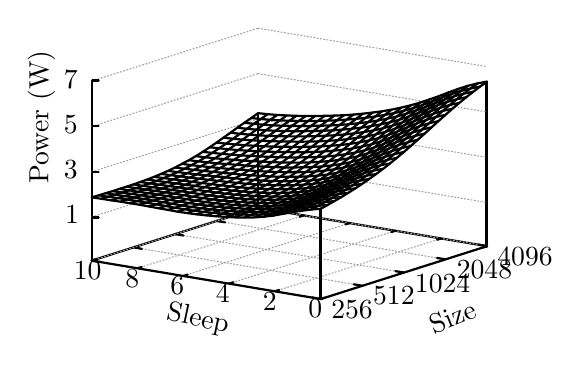
\begin{tikzpicture}[y=0.80pt, x=0.80pt, yscale=-0.570000, xscale=0.570000, inner sep=0pt, outer sep=0pt]
\begin{scope}[draw=black,line join=bevel,line cap=rect,even odd rule,line width=0.800pt]
  \begin{scope}[cm={{1.0,0.0,0.0,1.0,(0.0,0.0)}},draw=black,line join=bevel,line cap=rect,line width=0.800pt]
  \end{scope}
  \begin{scope}[cm={{1.00465,0.0,0.0,1.00465,(0.0,0.0)}},draw=black,line join=bevel,line cap=rect,line width=0.800pt]
  \end{scope}
  \begin{scope}[cm={{1.00465,0.0,0.0,1.00465,(0.0,0.0)}},draw=black,line join=round,line cap=round,line width=0.800pt]
    \path[draw] (59.1000,229.5000) -- (190.3000,187.8000);
    \path[draw] (370.9000,218.1000) -- (190.3000,187.8000);
    \path[draw] (59.5000,229.5000) -- (59.5000,87.5000);
    \path[draw] (190.5000,187.5000) -- (190.5000,113.5000);
    \path[draw] (370.5000,218.5000) -- (370.5000,88.5000);
  \end{scope}
  \begin{scope}[cm={{1.00465,0.0,0.0,1.00465,(0.0,0.0)}},draw=ca0a0a4,dash pattern=on 0.40pt off 0.80pt,line join=round,line cap=round,line width=0.400pt]
    \path[draw] (239.7000,259.8000) -- (59.1000,229.5000);
  \end{scope}
  \begin{scope}[cm={{1.00465,0.0,0.0,1.00465,(0.0,0.0)}},draw=black,line join=round,line cap=round,line width=0.800pt]
    \path[draw] (239.7000,259.8000) -- (232.9000,258.6000);
    \path[draw] (59.1000,229.5000) -- (65.8000,230.6000);
  \end{scope}
  \begin{scope}[cm={{1.00465,0.0,0.0,1.00465,(0.0,0.0)}},draw=black,line join=bevel,line cap=rect,line width=0.800pt]
  \end{scope}
  \begin{scope}[cm={{1.00465,0.0,0.0,1.00465,(249.153,276.781)}},draw=black,line join=bevel,line cap=rect,line width=0.800pt]
  \end{scope}
  \begin{scope}[cm={{1.00465,0.0,0.0,1.00465,(249.153,276.781)}},draw=black,line join=bevel,line cap=rect,line width=0.800pt]
  \end{scope}
  \begin{scope}[cm={{1.00465,0.0,0.0,1.00465,(249.153,276.781)}},draw=black,line join=bevel,line cap=rect,line width=0.800pt]
  \end{scope}
  \begin{scope}[cm={{1.00465,0.0,0.0,1.00465,(249.153,276.781)}},draw=black,line join=bevel,line cap=rect,line width=0.800pt]
  \end{scope}
  \begin{scope}[cm={{1.00465,0.0,0.0,1.00465,(249.153,276.781)}},draw=black,line join=bevel,line cap=rect,line width=0.800pt]
  \end{scope}
  \begin{scope}[cm={{1.00465,0.0,0.0,1.00465,(249.153,276.781)}},draw=black,line join=bevel,line cap=rect,line width=0.800pt]
    \path[fill=black] (0.0000,0.0000) node[above right] () {256};
  \end{scope}
  \begin{scope}[cm={{1.00465,0.0,0.0,1.00465,(249.153,276.781)}},draw=black,line join=bevel,line cap=rect,line width=0.800pt]
  \end{scope}
  \begin{scope}[cm={{1.00465,0.0,0.0,1.00465,(0.0,0.0)}},draw=black,line join=bevel,line cap=rect,line width=0.800pt]
  \end{scope}
  \begin{scope}[cm={{1.00465,0.0,0.0,1.00465,(0.0,0.0)}},draw=ca0a0a4,dash pattern=on 0.40pt off 0.80pt,line join=round,line cap=round,line width=0.400pt]
    \path[draw] (272.5000,249.3000) -- (91.9000,219.0000);
  \end{scope}
  \begin{scope}[cm={{1.00465,0.0,0.0,1.00465,(0.0,0.0)}},draw=black,line join=round,line cap=round,line width=0.800pt]
    \path[draw] (272.5000,249.3000) -- (265.8000,248.2000);
    \path[draw] (91.9000,219.0000) -- (98.6000,220.2000);
  \end{scope}
  \begin{scope}[cm={{1.00465,0.0,0.0,1.00465,(0.0,0.0)}},draw=black,line join=bevel,line cap=rect,line width=0.800pt]
  \end{scope}
  \begin{scope}[cm={{1.00465,0.0,0.0,1.00465,(282.307,265.73)}},draw=black,line join=bevel,line cap=rect,line width=0.800pt]
  \end{scope}
  \begin{scope}[cm={{1.00465,0.0,0.0,1.00465,(282.307,265.73)}},draw=black,line join=bevel,line cap=rect,line width=0.800pt]
  \end{scope}
  \begin{scope}[cm={{1.00465,0.0,0.0,1.00465,(282.307,265.73)}},draw=black,line join=bevel,line cap=rect,line width=0.800pt]
  \end{scope}
  \begin{scope}[cm={{1.00465,0.0,0.0,1.00465,(282.307,265.73)}},draw=black,line join=bevel,line cap=rect,line width=0.800pt]
  \end{scope}
  \begin{scope}[cm={{1.00465,0.0,0.0,1.00465,(282.307,265.73)}},draw=black,line join=bevel,line cap=rect,line width=0.800pt]
  \end{scope}
  \begin{scope}[cm={{1.00465,0.0,0.0,1.00465,(282.307,265.73)}},draw=black,line join=bevel,line cap=rect,line width=0.800pt]
    \path[fill=black] (0.0000,0.0000) node[above right] () {512};
  \end{scope}
  \begin{scope}[cm={{1.00465,0.0,0.0,1.00465,(282.307,265.73)}},draw=black,line join=bevel,line cap=rect,line width=0.800pt]
  \end{scope}
  \begin{scope}[cm={{1.00465,0.0,0.0,1.00465,(0.0,0.0)}},draw=black,line join=bevel,line cap=rect,line width=0.800pt]
  \end{scope}
  \begin{scope}[cm={{1.00465,0.0,0.0,1.00465,(0.0,0.0)}},draw=ca0a0a4,dash pattern=on 0.40pt off 0.80pt,line join=round,line cap=round,line width=0.400pt]
    \path[draw] (305.3000,238.9000) -- (124.7000,208.6000);
  \end{scope}
  \begin{scope}[cm={{1.00465,0.0,0.0,1.00465,(0.0,0.0)}},draw=black,line join=round,line cap=round,line width=0.800pt]
    \path[draw] (305.3000,238.9000) -- (298.6000,237.8000);
    \path[draw] (124.7000,208.6000) -- (131.4000,209.7000);
  \end{scope}
  \begin{scope}[cm={{1.00465,0.0,0.0,1.00465,(0.0,0.0)}},draw=black,line join=bevel,line cap=rect,line width=0.800pt]
  \end{scope}
  \begin{scope}[cm={{1.00465,0.0,0.0,1.00465,(315.46,255.684)}},draw=black,line join=bevel,line cap=rect,line width=0.800pt]
  \end{scope}
  \begin{scope}[cm={{1.00465,0.0,0.0,1.00465,(315.46,255.684)}},draw=black,line join=bevel,line cap=rect,line width=0.800pt]
  \end{scope}
  \begin{scope}[cm={{1.00465,0.0,0.0,1.00465,(315.46,255.684)}},draw=black,line join=bevel,line cap=rect,line width=0.800pt]
  \end{scope}
  \begin{scope}[cm={{1.00465,0.0,0.0,1.00465,(315.46,255.684)}},draw=black,line join=bevel,line cap=rect,line width=0.800pt]
  \end{scope}
  \begin{scope}[cm={{1.00465,0.0,0.0,1.00465,(315.46,255.684)}},draw=black,line join=bevel,line cap=rect,line width=0.800pt]
  \end{scope}
  \begin{scope}[cm={{1.00465,0.0,0.0,1.00465,(315.46,255.684)}},draw=black,line join=bevel,line cap=rect,line width=0.800pt]
    \path[fill=black] (0.0000,0.0000) node[above right] () {1024};
  \end{scope}
  \begin{scope}[cm={{1.00465,0.0,0.0,1.00465,(315.46,255.684)}},draw=black,line join=bevel,line cap=rect,line width=0.800pt]
  \end{scope}
  \begin{scope}[cm={{1.00465,0.0,0.0,1.00465,(0.0,0.0)}},draw=black,line join=bevel,line cap=rect,line width=0.800pt]
  \end{scope}
  \begin{scope}[cm={{1.00465,0.0,0.0,1.00465,(0.0,0.0)}},draw=ca0a0a4,dash pattern=on 0.40pt off 0.80pt,line join=round,line cap=round,line width=0.400pt]
    \path[draw] (338.1000,228.5000) -- (157.5000,198.2000);
  \end{scope}
  \begin{scope}[cm={{1.00465,0.0,0.0,1.00465,(0.0,0.0)}},draw=black,line join=round,line cap=round,line width=0.800pt]
    \path[draw] (338.1000,228.5000) -- (331.4000,227.4000);
    \path[draw] (157.5000,198.2000) -- (164.2000,199.3000);
  \end{scope}
  \begin{scope}[cm={{1.00465,0.0,0.0,1.00465,(0.0,0.0)}},draw=black,line join=bevel,line cap=rect,line width=0.800pt]
  \end{scope}
  \begin{scope}[cm={{1.00465,0.0,0.0,1.00465,(348.614,244.633)}},draw=black,line join=bevel,line cap=rect,line width=0.800pt]
  \end{scope}
  \begin{scope}[cm={{1.00465,0.0,0.0,1.00465,(348.614,244.633)}},draw=black,line join=bevel,line cap=rect,line width=0.800pt]
  \end{scope}
  \begin{scope}[cm={{1.00465,0.0,0.0,1.00465,(348.614,244.633)}},draw=black,line join=bevel,line cap=rect,line width=0.800pt]
  \end{scope}
  \begin{scope}[cm={{1.00465,0.0,0.0,1.00465,(348.614,244.633)}},draw=black,line join=bevel,line cap=rect,line width=0.800pt]
  \end{scope}
  \begin{scope}[cm={{1.00465,0.0,0.0,1.00465,(348.614,244.633)}},draw=black,line join=bevel,line cap=rect,line width=0.800pt]
  \end{scope}
  \begin{scope}[cm={{1.00465,0.0,0.0,1.00465,(348.614,244.633)}},draw=black,line join=bevel,line cap=rect,line width=0.800pt]
    \path[fill=black] (0.0000,0.0000) node[above right] () {2048};
  \end{scope}
  \begin{scope}[cm={{1.00465,0.0,0.0,1.00465,(348.614,244.633)}},draw=black,line join=bevel,line cap=rect,line width=0.800pt]
  \end{scope}
  \begin{scope}[cm={{1.00465,0.0,0.0,1.00465,(0.0,0.0)}},draw=black,line join=bevel,line cap=rect,line width=0.800pt]
  \end{scope}
  \begin{scope}[cm={{1.00465,0.0,0.0,1.00465,(0.0,0.0)}},draw=ca0a0a4,dash pattern=on 0.40pt off 0.80pt,line join=round,line cap=round,line width=0.400pt]
    \path[draw] (370.9000,218.1000) -- (190.3000,187.8000);
  \end{scope}
  \begin{scope}[cm={{1.00465,0.0,0.0,1.00465,(0.0,0.0)}},draw=black,line join=round,line cap=round,line width=0.800pt]
    \path[draw] (370.9000,218.1000) -- (364.2000,216.9000);
    \path[draw] (190.3000,187.8000) -- (197.1000,188.9000);
  \end{scope}
  \begin{scope}[cm={{1.00465,0.0,0.0,1.00465,(0.0,0.0)}},draw=black,line join=bevel,line cap=rect,line width=0.800pt]
  \end{scope}
  \begin{scope}[cm={{1.00465,0.0,0.0,1.00465,(380.763,234.586)}},draw=black,line join=bevel,line cap=rect,line width=0.800pt]
  \end{scope}
  \begin{scope}[cm={{1.00465,0.0,0.0,1.00465,(380.763,234.586)}},draw=black,line join=bevel,line cap=rect,line width=0.800pt]
  \end{scope}
  \begin{scope}[cm={{1.00465,0.0,0.0,1.00465,(380.763,234.586)}},draw=black,line join=bevel,line cap=rect,line width=0.800pt]
  \end{scope}
  \begin{scope}[cm={{1.00465,0.0,0.0,1.00465,(380.763,234.586)}},draw=black,line join=bevel,line cap=rect,line width=0.800pt]
  \end{scope}
  \begin{scope}[cm={{1.00465,0.0,0.0,1.00465,(380.763,234.586)}},draw=black,line join=bevel,line cap=rect,line width=0.800pt]
  \end{scope}
  \begin{scope}[cm={{1.00465,0.0,0.0,1.00465,(380.763,234.586)}},draw=black,line join=bevel,line cap=rect,line width=0.800pt]
    \path[fill=black] (0.0000,0.0000) node[above right] () {4096};
  \end{scope}
  \begin{scope}[cm={{1.00465,0.0,0.0,1.00465,(380.763,234.586)}},draw=black,line join=bevel,line cap=rect,line width=0.800pt]
  \end{scope}
  \begin{scope}[cm={{1.00465,0.0,0.0,1.00465,(0.0,0.0)}},draw=black,line join=bevel,line cap=rect,line width=0.800pt]
  \end{scope}
  \begin{scope}[cm={{1.00465,0.0,0.0,1.00465,(0.0,0.0)}},draw=ca0a0a4,dash pattern=on 0.40pt off 0.80pt,line join=round,line cap=round,line width=0.400pt]
    \path[draw] (239.7000,259.8000) -- (370.9000,218.1000);
  \end{scope}
  \begin{scope}[cm={{1.00465,0.0,0.0,1.00465,(0.0,0.0)}},draw=black,line join=round,line cap=round,line width=0.800pt]
    \path[draw] (239.7000,259.8000) -- (242.9000,258.7000);
    \path[draw] (370.9000,218.1000) -- (367.6000,219.1000);
  \end{scope}
  \begin{scope}[cm={{1.00465,0.0,0.0,1.00465,(0.0,0.0)}},draw=black,line join=bevel,line cap=rect,line width=0.800pt]
  \end{scope}
  \begin{scope}[cm={{1.00465,0.0,0.0,1.00465,(231.07,275.777)}},draw=black,line join=bevel,line cap=rect,line width=0.800pt]
  \end{scope}
  \begin{scope}[cm={{1.00465,0.0,0.0,1.00465,(231.07,275.777)}},draw=black,line join=bevel,line cap=rect,line width=0.800pt]
  \end{scope}
  \begin{scope}[cm={{1.00465,0.0,0.0,1.00465,(231.07,275.777)}},draw=black,line join=bevel,line cap=rect,line width=0.800pt]
  \end{scope}
  \begin{scope}[cm={{1.00465,0.0,0.0,1.00465,(231.07,275.777)}},draw=black,line join=bevel,line cap=rect,line width=0.800pt]
  \end{scope}
  \begin{scope}[cm={{1.00465,0.0,0.0,1.00465,(231.07,275.777)}},draw=black,line join=bevel,line cap=rect,line width=0.800pt]
  \end{scope}
  \begin{scope}[cm={{1.00465,0.0,0.0,1.00465,(231.07,275.777)}},draw=black,line join=bevel,line cap=rect,line width=0.800pt]
    \path[fill=black] (0.0000,0.0000) node[above right] () {0};
  \end{scope}
  \begin{scope}[cm={{1.00465,0.0,0.0,1.00465,(231.07,275.777)}},draw=black,line join=bevel,line cap=rect,line width=0.800pt]
  \end{scope}
  \begin{scope}[cm={{1.00465,0.0,0.0,1.00465,(0.0,0.0)}},draw=black,line join=bevel,line cap=rect,line width=0.800pt]
  \end{scope}
  \begin{scope}[cm={{1.00465,0.0,0.0,1.00465,(0.0,0.0)}},draw=ca0a0a4,dash pattern=on 0.40pt off 0.80pt,line join=round,line cap=round,line width=0.400pt]
    \path[draw] (203.6000,253.7000) -- (334.8000,212.0000);
  \end{scope}
  \begin{scope}[cm={{1.00465,0.0,0.0,1.00465,(0.0,0.0)}},draw=black,line join=round,line cap=round,line width=0.800pt]
    \path[draw] (203.6000,253.7000) -- (206.9000,252.6000);
    \path[draw] (334.8000,212.0000) -- (331.5000,213.0000);
  \end{scope}
  \begin{scope}[cm={{1.00465,0.0,0.0,1.00465,(0.0,0.0)}},draw=black,line join=bevel,line cap=rect,line width=0.800pt]
  \end{scope}
  \begin{scope}[cm={{1.00465,0.0,0.0,1.00465,(194.902,269.749)}},draw=black,line join=bevel,line cap=rect,line width=0.800pt]
  \end{scope}
  \begin{scope}[cm={{1.00465,0.0,0.0,1.00465,(194.902,269.749)}},draw=black,line join=bevel,line cap=rect,line width=0.800pt]
  \end{scope}
  \begin{scope}[cm={{1.00465,0.0,0.0,1.00465,(194.902,269.749)}},draw=black,line join=bevel,line cap=rect,line width=0.800pt]
  \end{scope}
  \begin{scope}[cm={{1.00465,0.0,0.0,1.00465,(194.902,269.749)}},draw=black,line join=bevel,line cap=rect,line width=0.800pt]
  \end{scope}
  \begin{scope}[cm={{1.00465,0.0,0.0,1.00465,(194.902,269.749)}},draw=black,line join=bevel,line cap=rect,line width=0.800pt]
  \end{scope}
  \begin{scope}[cm={{1.00465,0.0,0.0,1.00465,(194.902,269.749)}},draw=black,line join=bevel,line cap=rect,line width=0.800pt]
    \path[fill=black] (0.0000,0.0000) node[above right] () {2};
  \end{scope}
  \begin{scope}[cm={{1.00465,0.0,0.0,1.00465,(194.902,269.749)}},draw=black,line join=bevel,line cap=rect,line width=0.800pt]
  \end{scope}
  \begin{scope}[cm={{1.00465,0.0,0.0,1.00465,(0.0,0.0)}},draw=black,line join=bevel,line cap=rect,line width=0.800pt]
  \end{scope}
  \begin{scope}[cm={{1.00465,0.0,0.0,1.00465,(0.0,0.0)}},draw=ca0a0a4,dash pattern=on 0.40pt off 0.80pt,line join=round,line cap=round,line width=0.400pt]
    \path[draw] (167.5000,247.6000) -- (298.6000,205.9000);
  \end{scope}
  \begin{scope}[cm={{1.00465,0.0,0.0,1.00465,(0.0,0.0)}},draw=black,line join=round,line cap=round,line width=0.800pt]
    \path[draw] (167.5000,247.6000) -- (170.8000,246.6000);
    \path[draw] (298.6000,205.9000) -- (295.3000,207.0000);
  \end{scope}
  \begin{scope}[cm={{1.00465,0.0,0.0,1.00465,(0.0,0.0)}},draw=black,line join=bevel,line cap=rect,line width=0.800pt]
  \end{scope}
  \begin{scope}[cm={{1.00465,0.0,0.0,1.00465,(157.73,263.721)}},draw=black,line join=bevel,line cap=rect,line width=0.800pt]
  \end{scope}
  \begin{scope}[cm={{1.00465,0.0,0.0,1.00465,(157.73,263.721)}},draw=black,line join=bevel,line cap=rect,line width=0.800pt]
  \end{scope}
  \begin{scope}[cm={{1.00465,0.0,0.0,1.00465,(157.73,263.721)}},draw=black,line join=bevel,line cap=rect,line width=0.800pt]
  \end{scope}
  \begin{scope}[cm={{1.00465,0.0,0.0,1.00465,(157.73,263.721)}},draw=black,line join=bevel,line cap=rect,line width=0.800pt]
  \end{scope}
  \begin{scope}[cm={{1.00465,0.0,0.0,1.00465,(157.73,263.721)}},draw=black,line join=bevel,line cap=rect,line width=0.800pt]
  \end{scope}
  \begin{scope}[cm={{1.00465,0.0,0.0,1.00465,(157.73,263.721)}},draw=black,line join=bevel,line cap=rect,line width=0.800pt]
    \path[fill=black] (0.0000,0.0000) node[above right] () {4};
  \end{scope}
  \begin{scope}[cm={{1.00465,0.0,0.0,1.00465,(157.73,263.721)}},draw=black,line join=bevel,line cap=rect,line width=0.800pt]
  \end{scope}
  \begin{scope}[cm={{1.00465,0.0,0.0,1.00465,(0.0,0.0)}},draw=black,line join=bevel,line cap=rect,line width=0.800pt]
  \end{scope}
  \begin{scope}[cm={{1.00465,0.0,0.0,1.00465,(0.0,0.0)}},draw=ca0a0a4,dash pattern=on 0.40pt off 0.80pt,line join=round,line cap=round,line width=0.400pt]
    \path[draw] (131.4000,241.6000) -- (262.5000,199.9000);
  \end{scope}
  \begin{scope}[cm={{1.00465,0.0,0.0,1.00465,(0.0,0.0)}},draw=black,line join=round,line cap=round,line width=0.800pt]
    \path[draw] (131.4000,241.6000) -- (134.7000,240.5000);
    \path[draw] (262.5000,199.9000) -- (259.2000,200.9000);
  \end{scope}
  \begin{scope}[cm={{1.00465,0.0,0.0,1.00465,(0.0,0.0)}},draw=black,line join=bevel,line cap=rect,line width=0.800pt]
  \end{scope}
  \begin{scope}[cm={{1.00465,0.0,0.0,1.00465,(121.563,257.693)}},draw=black,line join=bevel,line cap=rect,line width=0.800pt]
  \end{scope}
  \begin{scope}[cm={{1.00465,0.0,0.0,1.00465,(121.563,257.693)}},draw=black,line join=bevel,line cap=rect,line width=0.800pt]
  \end{scope}
  \begin{scope}[cm={{1.00465,0.0,0.0,1.00465,(121.563,257.693)}},draw=black,line join=bevel,line cap=rect,line width=0.800pt]
  \end{scope}
  \begin{scope}[cm={{1.00465,0.0,0.0,1.00465,(121.563,257.693)}},draw=black,line join=bevel,line cap=rect,line width=0.800pt]
  \end{scope}
  \begin{scope}[cm={{1.00465,0.0,0.0,1.00465,(121.563,257.693)}},draw=black,line join=bevel,line cap=rect,line width=0.800pt]
  \end{scope}
  \begin{scope}[cm={{1.00465,0.0,0.0,1.00465,(121.563,257.693)}},draw=black,line join=bevel,line cap=rect,line width=0.800pt]
    \path[fill=black] (0.0000,0.0000) node[above right] () {6};
  \end{scope}
  \begin{scope}[cm={{1.00465,0.0,0.0,1.00465,(121.563,257.693)}},draw=black,line join=bevel,line cap=rect,line width=0.800pt]
  \end{scope}
  \begin{scope}[cm={{1.00465,0.0,0.0,1.00465,(0.0,0.0)}},draw=black,line join=bevel,line cap=rect,line width=0.800pt]
  \end{scope}
  \begin{scope}[cm={{1.00465,0.0,0.0,1.00465,(0.0,0.0)}},draw=ca0a0a4,dash pattern=on 0.40pt off 0.80pt,line join=round,line cap=round,line width=0.400pt]
    \path[draw] (95.2000,235.5000) -- (226.4000,193.8000);
  \end{scope}
  \begin{scope}[cm={{1.00465,0.0,0.0,1.00465,(0.0,0.0)}},draw=black,line join=round,line cap=round,line width=0.800pt]
    \path[draw] (95.2000,235.5000) -- (98.5000,234.5000);
    \path[draw] (226.4000,193.8000) -- (223.1000,194.9000);
  \end{scope}
  \begin{scope}[cm={{1.00465,0.0,0.0,1.00465,(0.0,0.0)}},draw=black,line join=bevel,line cap=rect,line width=0.800pt]
  \end{scope}
  \begin{scope}[cm={{1.00465,0.0,0.0,1.00465,(85.8977,251.665)}},draw=black,line join=bevel,line cap=rect,line width=0.800pt]
  \end{scope}
  \begin{scope}[cm={{1.00465,0.0,0.0,1.00465,(85.8977,251.665)}},draw=black,line join=bevel,line cap=rect,line width=0.800pt]
  \end{scope}
  \begin{scope}[cm={{1.00465,0.0,0.0,1.00465,(85.8977,251.665)}},draw=black,line join=bevel,line cap=rect,line width=0.800pt]
  \end{scope}
  \begin{scope}[cm={{1.00465,0.0,0.0,1.00465,(85.8977,251.665)}},draw=black,line join=bevel,line cap=rect,line width=0.800pt]
  \end{scope}
  \begin{scope}[cm={{1.00465,0.0,0.0,1.00465,(85.8977,251.665)}},draw=black,line join=bevel,line cap=rect,line width=0.800pt]
  \end{scope}
  \begin{scope}[cm={{1.00465,0.0,0.0,1.00465,(85.8977,251.665)}},draw=black,line join=bevel,line cap=rect,line width=0.800pt]
    \path[fill=black] (0.0000,0.0000) node[above right] () {8};
  \end{scope}
  \begin{scope}[cm={{1.00465,0.0,0.0,1.00465,(85.8977,251.665)}},draw=black,line join=bevel,line cap=rect,line width=0.800pt]
  \end{scope}
  \begin{scope}[cm={{1.00465,0.0,0.0,1.00465,(0.0,0.0)}},draw=black,line join=bevel,line cap=rect,line width=0.800pt]
  \end{scope}
  \begin{scope}[cm={{1.00465,0.0,0.0,1.00465,(0.0,0.0)}},draw=ca0a0a4,dash pattern=on 0.40pt off 0.80pt,line join=round,line cap=round,line width=0.400pt]
    \path[draw] (59.1000,229.5000) -- (190.3000,187.8000);
  \end{scope}
  \begin{scope}[cm={{1.00465,0.0,0.0,1.00465,(0.0,0.0)}},draw=black,line join=round,line cap=round,line width=0.800pt]
    \path[draw] (59.1000,229.5000) -- (62.4000,228.4000);
    \path[draw] (190.3000,187.8000) -- (187.1000,188.8000);
  \end{scope}
  \begin{scope}[cm={{1.00465,0.0,0.0,1.00465,(0.0,0.0)}},draw=black,line join=bevel,line cap=rect,line width=0.800pt]
  \end{scope}
  \begin{scope}[cm={{1.00465,0.0,0.0,1.00465,(45.2093,245.637)}},draw=black,line join=bevel,line cap=rect,line width=0.800pt]
  \end{scope}
  \begin{scope}[cm={{1.00465,0.0,0.0,1.00465,(45.2093,245.637)}},draw=black,line join=bevel,line cap=rect,line width=0.800pt]
  \end{scope}
  \begin{scope}[cm={{1.00465,0.0,0.0,1.00465,(45.2093,245.637)}},draw=black,line join=bevel,line cap=rect,line width=0.800pt]
  \end{scope}
  \begin{scope}[cm={{1.00465,0.0,0.0,1.00465,(45.2093,245.637)}},draw=black,line join=bevel,line cap=rect,line width=0.800pt]
  \end{scope}
  \begin{scope}[cm={{1.00465,0.0,0.0,1.00465,(45.2093,245.637)}},draw=black,line join=bevel,line cap=rect,line width=0.800pt]
  \end{scope}
  \begin{scope}[cm={{1.00465,0.0,0.0,1.00465,(45.2093,245.637)}},draw=black,line join=bevel,line cap=rect,line width=0.800pt]
    \path[fill=black] (0.0000,0.0000) node[above right] () {10};
  \end{scope}
  \begin{scope}[cm={{1.00465,0.0,0.0,1.00465,(45.2093,245.637)}},draw=black,line join=bevel,line cap=rect,line width=0.800pt]
  \end{scope}
  \begin{scope}[cm={{1.00465,0.0,0.0,1.00465,(0.0,0.0)}},draw=black,line join=bevel,line cap=rect,line width=0.800pt]
  \end{scope}
  \begin{scope}[cm={{1.00465,0.0,0.0,1.00465,(0.0,0.0)}},draw=ca0a0a4,dash pattern=on 0.40pt off 0.80pt,line join=round,line cap=round,line width=0.400pt]
    \path[draw] (59.1000,195.1000) -- (190.3000,153.4000);
    \path[draw] (190.3000,153.4000) -- (190.3000,153.4000) -- (370.9000,183.7000);
  \end{scope}
  \begin{scope}[cm={{1.00465,0.0,0.0,1.00465,(0.0,0.0)}},draw=black,line join=round,line cap=round,line width=0.800pt]
    \path[draw] (59.5000,195.5000) -- (64.5000,195.5000);
  \end{scope}
  \begin{scope}[cm={{1.00465,0.0,0.0,1.00465,(0.0,0.0)}},draw=black,line join=bevel,line cap=rect,line width=0.800pt]
  \end{scope}
  \begin{scope}[cm={{1.00465,0.0,0.0,1.00465,(38.1767,201.433)}},draw=black,line join=bevel,line cap=rect,line width=0.800pt]
  \end{scope}
  \begin{scope}[cm={{1.00465,0.0,0.0,1.00465,(38.1767,201.433)}},draw=black,line join=bevel,line cap=rect,line width=0.800pt]
  \end{scope}
  \begin{scope}[cm={{1.00465,0.0,0.0,1.00465,(38.1767,201.433)}},draw=black,line join=bevel,line cap=rect,line width=0.800pt]
  \end{scope}
  \begin{scope}[cm={{1.00465,0.0,0.0,1.00465,(38.1767,201.433)}},draw=black,line join=bevel,line cap=rect,line width=0.800pt]
  \end{scope}
  \begin{scope}[cm={{1.00465,0.0,0.0,1.00465,(38.1767,201.433)}},draw=black,line join=bevel,line cap=rect,line width=0.800pt]
  \end{scope}
  \begin{scope}[cm={{1.00465,0.0,0.0,1.00465,(38.1767,201.433)}},draw=black,line join=bevel,line cap=rect,line width=0.800pt]
    \path[fill=black] (0.0000,0.0000) node[above right] () {1};
  \end{scope}
  \begin{scope}[cm={{1.00465,0.0,0.0,1.00465,(38.1767,201.433)}},draw=black,line join=bevel,line cap=rect,line width=0.800pt]
  \end{scope}
  \begin{scope}[cm={{1.00465,0.0,0.0,1.00465,(0.0,0.0)}},draw=black,line join=bevel,line cap=rect,line width=0.800pt]
  \end{scope}
  \begin{scope}[cm={{1.00465,0.0,0.0,1.00465,(0.0,0.0)}},draw=ca0a0a4,dash pattern=on 0.40pt off 0.80pt,line join=round,line cap=round,line width=0.400pt]
    \path[draw] (59.1000,159.4000) -- (190.3000,117.8000);
    \path[draw] (190.3000,117.8000) -- (190.3000,117.8000) -- (370.9000,148.1000);
  \end{scope}
  \begin{scope}[cm={{1.00465,0.0,0.0,1.00465,(0.0,0.0)}},draw=black,line join=round,line cap=round,line width=0.800pt]
    \path[draw] (59.5000,159.5000) -- (64.5000,159.5000);
  \end{scope}
  \begin{scope}[cm={{1.00465,0.0,0.0,1.00465,(0.0,0.0)}},draw=black,line join=bevel,line cap=rect,line width=0.800pt]
  \end{scope}
  \begin{scope}[cm={{1.00465,0.0,0.0,1.00465,(37.1721,165.265)}},draw=black,line join=bevel,line cap=rect,line width=0.800pt]
  \end{scope}
  \begin{scope}[cm={{1.00465,0.0,0.0,1.00465,(37.1721,165.265)}},draw=black,line join=bevel,line cap=rect,line width=0.800pt]
  \end{scope}
  \begin{scope}[cm={{1.00465,0.0,0.0,1.00465,(37.1721,165.265)}},draw=black,line join=bevel,line cap=rect,line width=0.800pt]
  \end{scope}
  \begin{scope}[cm={{1.00465,0.0,0.0,1.00465,(37.1721,165.265)}},draw=black,line join=bevel,line cap=rect,line width=0.800pt]
  \end{scope}
  \begin{scope}[cm={{1.00465,0.0,0.0,1.00465,(37.1721,165.265)}},draw=black,line join=bevel,line cap=rect,line width=0.800pt]
  \end{scope}
  \begin{scope}[cm={{1.00465,0.0,0.0,1.00465,(37.1721,165.265)}},draw=black,line join=bevel,line cap=rect,line width=0.800pt]
    \path[fill=black] (0.0000,0.0000) node[above right] () {3};
  \end{scope}
  \begin{scope}[cm={{1.00465,0.0,0.0,1.00465,(37.1721,165.265)}},draw=black,line join=bevel,line cap=rect,line width=0.800pt]
  \end{scope}
  \begin{scope}[cm={{1.00465,0.0,0.0,1.00465,(0.0,0.0)}},draw=black,line join=bevel,line cap=rect,line width=0.800pt]
  \end{scope}
  \begin{scope}[cm={{1.00465,0.0,0.0,1.00465,(0.0,0.0)}},draw=ca0a0a4,dash pattern=on 0.40pt off 0.80pt,line join=round,line cap=round,line width=0.400pt]
    \path[draw] (59.1000,123.7000) -- (190.3000,82.0000);
    \path[draw] (190.3000,82.0000) -- (190.3000,82.0000) -- (370.9000,112.3000);
  \end{scope}
  \begin{scope}[cm={{1.00465,0.0,0.0,1.00465,(0.0,0.0)}},draw=black,line join=round,line cap=round,line width=0.800pt]
    \path[draw] (59.5000,123.5000) -- (64.5000,123.5000);
  \end{scope}
  \begin{scope}[cm={{1.00465,0.0,0.0,1.00465,(0.0,0.0)}},draw=black,line join=bevel,line cap=rect,line width=0.800pt]
  \end{scope}
  \begin{scope}[cm={{1.00465,0.0,0.0,1.00465,(37.1721,130.102)}},draw=black,line join=bevel,line cap=rect,line width=0.800pt]
  \end{scope}
  \begin{scope}[cm={{1.00465,0.0,0.0,1.00465,(37.1721,130.102)}},draw=black,line join=bevel,line cap=rect,line width=0.800pt]
  \end{scope}
  \begin{scope}[cm={{1.00465,0.0,0.0,1.00465,(37.1721,130.102)}},draw=black,line join=bevel,line cap=rect,line width=0.800pt]
  \end{scope}
  \begin{scope}[cm={{1.00465,0.0,0.0,1.00465,(37.1721,130.102)}},draw=black,line join=bevel,line cap=rect,line width=0.800pt]
  \end{scope}
  \begin{scope}[cm={{1.00465,0.0,0.0,1.00465,(37.1721,130.102)}},draw=black,line join=bevel,line cap=rect,line width=0.800pt]
  \end{scope}
  \begin{scope}[cm={{1.00465,0.0,0.0,1.00465,(37.1721,130.102)}},draw=black,line join=bevel,line cap=rect,line width=0.800pt]
    \path[fill=black] (0.0000,0.0000) node[above right] () {5};
  \end{scope}
  \begin{scope}[cm={{1.00465,0.0,0.0,1.00465,(37.1721,130.102)}},draw=black,line join=bevel,line cap=rect,line width=0.800pt]
  \end{scope}
  \begin{scope}[cm={{1.00465,0.0,0.0,1.00465,(0.0,0.0)}},draw=black,line join=bevel,line cap=rect,line width=0.800pt]
  \end{scope}
  \begin{scope}[cm={{1.00465,0.0,0.0,1.00465,(0.0,0.0)}},draw=ca0a0a4,dash pattern=on 0.40pt off 0.80pt,line join=round,line cap=round,line width=0.400pt]
    \path[draw] (59.1000,87.9000) -- (190.3000,46.2000);
    \path[draw] (190.3000,46.2000) -- (190.3000,46.2000) -- (370.9000,76.5000);
  \end{scope}
  \begin{scope}[cm={{1.00465,0.0,0.0,1.00465,(0.0,0.0)}},draw=black,line join=round,line cap=round,line width=0.800pt]
    \path[draw] (59.5000,87.5000) -- (64.5000,87.5000);
  \end{scope}
  \begin{scope}[cm={{1.00465,0.0,0.0,1.00465,(0.0,0.0)}},draw=black,line join=bevel,line cap=rect,line width=0.800pt]
  \end{scope}
  \begin{scope}[cm={{1.00465,0.0,0.0,1.00465,(37.1721,93.9349)}},draw=black,line join=bevel,line cap=rect,line width=0.800pt]
  \end{scope}
  \begin{scope}[cm={{1.00465,0.0,0.0,1.00465,(37.1721,93.9349)}},draw=black,line join=bevel,line cap=rect,line width=0.800pt]
  \end{scope}
  \begin{scope}[cm={{1.00465,0.0,0.0,1.00465,(37.1721,93.9349)}},draw=black,line join=bevel,line cap=rect,line width=0.800pt]
  \end{scope}
  \begin{scope}[cm={{1.00465,0.0,0.0,1.00465,(37.1721,93.9349)}},draw=black,line join=bevel,line cap=rect,line width=0.800pt]
  \end{scope}
  \begin{scope}[cm={{1.00465,0.0,0.0,1.00465,(37.1721,93.9349)}},draw=black,line join=bevel,line cap=rect,line width=0.800pt]
  \end{scope}
  \begin{scope}[cm={{1.00465,0.0,0.0,1.00465,(37.1721,93.9349)}},draw=black,line join=bevel,line cap=rect,line width=0.800pt]
    \path[fill=black] (0.0000,0.0000) node[above right] () {7};
  \end{scope}
  \begin{scope}[cm={{1.00465,0.0,0.0,1.00465,(37.1721,93.9349)}},draw=black,line join=bevel,line cap=rect,line width=0.800pt]
  \end{scope}
  \begin{scope}[cm={{0.0,-1.00465,1.00465,0.0,(15.5721,176.316)}},draw=black,line join=bevel,line cap=rect,line width=0.800pt]
  \end{scope}
  \begin{scope}[cm={{0.0,-1.00465,1.00465,0.0,(15.5721,176.316)}},draw=black,line join=bevel,line cap=rect,line width=0.800pt]
  \end{scope}
  \begin{scope}[cm={{0.0,-1.00465,1.00465,0.0,(15.5721,176.316)}},draw=black,line join=bevel,line cap=rect,line width=0.800pt]
  \end{scope}
  \begin{scope}[cm={{0.0,-1.00465,1.00465,0.0,(15.5721,176.316)}},draw=black,line join=bevel,line cap=rect,line width=0.800pt]
  \end{scope}
  \begin{scope}[cm={{0.0,-1.00465,1.00465,0.0,(15.5721,176.316)}},draw=black,line join=bevel,line cap=rect,line width=0.800pt]
  \end{scope}
  \begin{scope}[cm={{0.0,-1.00465,1.00465,0.0,(8.5721,169.284)}},draw=black,line join=bevel,line cap=rect,line width=0.800pt]
    \path[fill=black] (0.0000,0.0000) node[above right] () {\rotatebox{90}{Power (W)}};
  \end{scope}
  \begin{scope}[cm={{0.0,-1.00465,1.00465,0.0,(15.5721,176.316)}},draw=black,line join=bevel,line cap=rect,line width=0.800pt]
  \end{scope}
  \begin{scope}[cm={{1.00465,0.0,0.0,1.00465,(0.0,0.0)}},draw=black,line join=bevel,line cap=rect,line width=0.800pt]
  \end{scope}
  \begin{scope}[cm={{1.00465,0.0,0.0,1.00465,(0.0,0.0)}},draw=black,line join=bevel,line cap=rect,line width=0.800pt]
  \end{scope}
  \begin{scope}[cm={{1.00465,0.0,0.0,1.00465,(0.0,0.0)}},draw=black,line join=bevel,line cap=rect,line width=0.800pt]
  \end{scope}
  \begin{scope}[cm={{1.00465,0.0,0.0,1.00465,(0.0,0.0)}},draw=black,line join=round,line cap=round,line width=0.800pt]
    \path[draw] (370.9000,88.3000) -- (363.4000,89.7000) -- (363.4000,89.7000) --
      (355.8000,91.6000) -- (355.8000,91.6000) -- (348.3000,94.0000) --
      (348.3000,94.0000) -- (340.8000,96.7000) -- (340.8000,96.7000) --
      (333.3000,99.6000) -- (333.3000,99.6000) -- (325.7000,102.3000) --
      (325.7000,102.3000) -- (318.2000,104.8000) -- (318.2000,104.8000) --
      (310.7000,107.0000) -- (310.7000,107.0000) -- (303.2000,108.8000) --
      (303.2000,108.8000) -- (295.6000,110.4000) -- (295.6000,110.4000) --
      (288.1000,111.7000) -- (288.1000,111.7000) -- (280.6000,112.7000) --
      (280.6000,112.7000) -- (273.0000,113.6000) -- (273.0000,113.6000) --
      (265.5000,114.3000) -- (265.5000,114.3000) -- (258.0000,114.8000) --
      (258.0000,114.8000) -- (250.5000,115.1000) -- (250.5000,115.1000) --
      (242.9000,115.3000) -- (242.9000,115.3000) -- (235.4000,115.4000) --
      (235.4000,115.4000) -- (227.9000,115.4000) -- (227.9000,115.4000) --
      (220.4000,115.3000) -- (220.4000,115.3000) -- (212.9000,115.0000) --
      (212.9000,115.0000) -- (205.4000,114.6000) -- (205.4000,114.6000) --
      (197.9000,114.0000) -- (197.9000,114.0000) -- (190.3000,113.2000);
    \path[draw] (365.4000,92.2000) -- (357.9000,93.7000) -- (357.9000,93.7000) --
      (350.4000,95.6000) -- (350.4000,95.6000) -- (342.9000,98.1000) --
      (342.9000,98.1000) -- (335.3000,100.9000) -- (335.3000,100.9000) --
      (327.8000,103.8000) -- (327.8000,103.8000) -- (320.3000,106.6000) --
      (320.3000,106.6000) -- (312.7000,109.2000) -- (312.7000,109.2000) --
      (305.2000,111.3000) -- (305.2000,111.3000) -- (297.7000,113.1000) --
      (297.7000,113.1000) -- (290.2000,114.6000) -- (290.2000,114.6000) --
      (282.6000,115.8000) -- (282.6000,115.8000) -- (275.1000,116.9000) --
      (275.1000,116.9000) -- (267.6000,117.7000) -- (267.6000,117.7000) --
      (260.1000,118.3000) -- (260.1000,118.3000) -- (252.5000,118.8000) --
      (252.5000,118.8000) -- (245.0000,119.1000) -- (245.0000,119.1000) --
      (237.5000,119.3000) -- (237.5000,119.3000) -- (229.9000,119.3000) --
      (229.9000,119.3000) -- (222.4000,119.3000) -- (222.4000,119.3000) --
      (215.0000,119.2000) -- (215.0000,119.2000) -- (207.5000,118.9000) --
      (207.5000,118.9000) -- (199.9000,118.4000) -- (199.9000,118.4000) --
      (192.4000,117.8000) -- (192.4000,117.8000) -- (184.9000,117.0000);
    \path[draw] (360.0000,96.3000) -- (352.4000,97.8000) -- (352.4000,97.8000) --
      (344.9000,99.9000) -- (344.9000,99.9000) -- (337.4000,102.4000) --
      (337.4000,102.4000) -- (329.9000,105.3000) -- (329.9000,105.3000) --
      (322.3000,108.3000) -- (322.3000,108.3000) -- (314.8000,111.1000) --
      (314.8000,111.1000) -- (307.3000,113.6000) -- (307.3000,113.6000) --
      (299.7000,115.8000) -- (299.7000,115.8000) -- (292.2000,117.5000) --
      (292.2000,117.5000) -- (284.7000,119.0000) -- (284.7000,119.0000) --
      (277.2000,120.2000) -- (277.2000,120.2000) -- (269.6000,121.1000) --
      (269.6000,121.1000) -- (262.1000,121.9000) -- (262.1000,121.9000) --
      (254.6000,122.5000) -- (254.6000,122.5000) -- (247.1000,122.9000) --
      (247.1000,122.9000) -- (239.5000,123.1000) -- (239.5000,123.1000) --
      (232.0000,123.3000) -- (232.0000,123.3000) -- (224.5000,123.3000) --
      (224.5000,123.3000) -- (216.9000,123.3000) -- (216.9000,123.3000) --
      (209.5000,123.1000) -- (209.5000,123.1000) -- (202.0000,122.8000) --
      (202.0000,122.8000) -- (194.5000,122.3000) -- (194.5000,122.3000) --
      (186.9000,121.6000) -- (186.9000,121.6000) -- (179.4000,120.8000);
    \path[draw] (354.5000,100.6000) -- (347.0000,102.2000) -- (347.0000,102.2000) --
      (339.4000,104.3000) -- (339.4000,104.3000) -- (331.9000,106.9000) --
      (331.9000,106.9000) -- (324.4000,109.9000) -- (324.4000,109.9000) --
      (316.9000,112.9000) -- (316.9000,112.9000) -- (309.3000,115.8000) --
      (309.3000,115.8000) -- (301.8000,118.3000) -- (301.8000,118.3000) --
      (294.3000,120.4000) -- (294.3000,120.4000) -- (286.8000,122.1000) --
      (286.8000,122.1000) -- (279.2000,123.5000) -- (279.2000,123.5000) --
      (271.7000,124.6000) -- (271.7000,124.6000) -- (264.2000,125.5000) --
      (264.2000,125.5000) -- (256.6000,126.2000) -- (256.6000,126.2000) --
      (249.1000,126.7000) -- (249.1000,126.7000) -- (241.6000,127.1000) --
      (241.6000,127.1000) -- (234.1000,127.3000) -- (234.1000,127.3000) --
      (226.5000,127.4000) -- (226.5000,127.4000) -- (219.0000,127.4000) --
      (219.0000,127.4000) -- (211.6000,127.3000) -- (211.6000,127.3000) --
      (204.1000,127.1000) -- (204.1000,127.1000) -- (196.5000,126.7000) --
      (196.5000,126.7000) -- (189.0000,126.2000) -- (189.0000,126.2000) --
      (181.5000,125.5000) -- (181.5000,125.5000) -- (173.9000,124.7000);
    \path[draw] (349.0000,105.1000) -- (341.5000,106.7000) -- (341.5000,106.7000) --
      (334.0000,108.9000) -- (334.0000,108.9000) -- (326.4000,111.6000) --
      (326.4000,111.6000) -- (318.9000,114.6000) -- (318.9000,114.6000) --
      (311.4000,117.7000) -- (311.4000,117.7000) -- (303.9000,120.6000) --
      (303.9000,120.6000) -- (296.3000,123.0000) -- (296.3000,123.0000) --
      (288.8000,125.1000) -- (288.8000,125.1000) -- (281.3000,126.8000) --
      (281.3000,126.8000) -- (273.8000,128.1000) -- (273.8000,128.1000) --
      (266.2000,129.1000) -- (266.2000,129.1000) -- (258.7000,130.0000) --
      (258.7000,130.0000) -- (251.2000,130.6000) -- (251.2000,130.6000) --
      (243.6000,131.0000) -- (243.6000,131.0000) -- (236.1000,131.3000) --
      (236.1000,131.3000) -- (228.6000,131.5000) -- (228.6000,131.5000) --
      (221.1000,131.5000) -- (221.1000,131.5000) -- (213.6000,131.5000) --
      (213.6000,131.5000) -- (206.1000,131.3000) -- (206.1000,131.3000) --
      (198.6000,131.1000) -- (198.6000,131.1000) -- (191.1000,130.7000) --
      (191.1000,130.7000) -- (183.5000,130.1000) -- (183.5000,130.1000) --
      (176.0000,129.5000) -- (176.0000,129.5000) -- (168.5000,128.6000);
    \path[draw] (343.6000,109.7000) -- (336.0000,111.4000) -- (336.0000,111.4000) --
      (328.5000,113.7000) -- (328.5000,113.7000) -- (321.0000,116.4000) --
      (321.0000,116.4000) -- (313.4000,119.5000) -- (313.4000,119.5000) --
      (305.9000,122.6000) -- (305.9000,122.6000) -- (298.4000,125.4000) --
      (298.4000,125.4000) -- (290.9000,127.9000) -- (290.9000,127.9000) --
      (283.3000,129.9000) -- (283.3000,129.9000) -- (275.8000,131.5000) --
      (275.8000,131.5000) -- (268.3000,132.7000) -- (268.3000,132.7000) --
      (260.8000,133.7000) -- (260.8000,133.7000) -- (253.2000,134.5000) --
      (253.2000,134.5000) -- (245.7000,135.0000) -- (245.7000,135.0000) --
      (238.2000,135.4000) -- (238.2000,135.4000) -- (230.7000,135.6000) --
      (230.7000,135.6000) -- (223.1000,135.7000) -- (223.1000,135.7000) --
      (215.6000,135.6000) -- (215.6000,135.6000) -- (208.2000,135.5000) --
      (208.2000,135.5000) -- (200.6000,135.3000) -- (200.6000,135.3000) --
      (193.1000,135.0000) -- (193.1000,135.0000) -- (185.6000,134.6000) --
      (185.6000,134.6000) -- (178.1000,134.1000) -- (178.1000,134.1000) --
      (170.5000,133.4000) -- (170.5000,133.4000) -- (163.0000,132.5000);
    \path[draw] (338.1000,114.5000) -- (330.6000,116.2000) -- (330.6000,116.2000) --
      (323.0000,118.5000) -- (323.0000,118.5000) -- (315.5000,121.3000) --
      (315.5000,121.3000) -- (308.0000,124.4000) -- (308.0000,124.4000) --
      (300.5000,127.5000) -- (300.5000,127.5000) -- (292.9000,130.4000) --
      (292.9000,130.4000) -- (285.4000,132.8000) -- (285.4000,132.8000) --
      (277.9000,134.7000) -- (277.9000,134.7000) -- (270.3000,136.2000) --
      (270.3000,136.2000) -- (262.8000,137.4000) -- (262.8000,137.4000) --
      (255.3000,138.3000) -- (255.3000,138.3000) -- (247.8000,138.9000) --
      (247.8000,138.9000) -- (240.2000,139.4000) -- (240.2000,139.4000) --
      (232.7000,139.7000) -- (232.7000,139.7000) -- (225.2000,139.8000) --
      (225.2000,139.8000) -- (217.7000,139.8000) -- (217.7000,139.8000) --
      (210.2000,139.7000) -- (210.2000,139.7000) -- (202.7000,139.6000) --
      (202.7000,139.6000) -- (195.2000,139.3000) -- (195.2000,139.3000) --
      (187.6000,138.9000) -- (187.6000,138.9000) -- (180.1000,138.5000) --
      (180.1000,138.5000) -- (172.6000,137.9000) -- (172.6000,137.9000) --
      (165.1000,137.2000) -- (165.1000,137.2000) -- (157.5000,136.4000);
    \path[draw] (332.6000,119.4000) -- (325.1000,121.2000) -- (325.1000,121.2000) --
      (317.6000,123.5000) -- (317.6000,123.5000) -- (310.0000,126.3000) --
      (310.0000,126.3000) -- (302.5000,129.4000) -- (302.5000,129.4000) --
      (295.0000,132.5000) -- (295.0000,132.5000) -- (287.5000,135.3000) --
      (287.5000,135.3000) -- (279.9000,137.7000) -- (279.9000,137.7000) --
      (272.4000,139.5000) -- (272.4000,139.5000) -- (264.9000,141.0000) --
      (264.9000,141.0000) -- (257.3000,142.0000) -- (257.3000,142.0000) --
      (249.8000,142.8000) -- (249.8000,142.8000) -- (242.3000,143.4000) --
      (242.3000,143.4000) -- (234.8000,143.8000) -- (234.8000,143.8000) --
      (227.2000,144.0000) -- (227.2000,144.0000) -- (219.7000,144.0000) --
      (219.7000,144.0000) -- (212.3000,143.9000) -- (212.3000,143.9000) --
      (204.8000,143.8000) -- (204.8000,143.8000) -- (197.2000,143.5000) --
      (197.2000,143.5000) -- (189.7000,143.2000) -- (189.7000,143.2000) --
      (182.2000,142.8000) -- (182.2000,142.8000) -- (174.6000,142.3000) --
      (174.6000,142.3000) -- (167.1000,141.7000) -- (167.1000,141.7000) --
      (159.6000,140.9000) -- (159.6000,140.9000) -- (152.1000,140.1000);
    \path[draw] (327.2000,124.3000) -- (319.6000,126.1000) -- (319.6000,126.1000) --
      (312.1000,128.4000) -- (312.1000,128.4000) -- (304.6000,131.3000) --
      (304.6000,131.3000) -- (297.0000,134.3000) -- (297.0000,134.3000) --
      (289.5000,137.4000) -- (289.5000,137.4000) -- (282.0000,140.2000) --
      (282.0000,140.2000) -- (274.5000,142.5000) -- (274.5000,142.5000) --
      (266.9000,144.3000) -- (266.9000,144.3000) -- (259.4000,145.6000) --
      (259.4000,145.6000) -- (251.9000,146.6000) -- (251.9000,146.6000) --
      (244.4000,147.3000) -- (244.4000,147.3000) -- (236.8000,147.8000) --
      (236.8000,147.8000) -- (229.3000,148.0000) -- (229.3000,148.0000) --
      (221.8000,148.1000) -- (221.8000,148.1000) -- (214.3000,148.1000) --
      (214.3000,148.1000) -- (206.8000,147.9000) -- (206.8000,147.9000) --
      (199.3000,147.7000) -- (199.3000,147.7000) -- (191.8000,147.3000) --
      (191.8000,147.3000) -- (184.2000,146.9000) -- (184.2000,146.9000) --
      (176.7000,146.5000) -- (176.7000,146.5000) -- (169.2000,145.9000) --
      (169.2000,145.9000) -- (161.7000,145.3000) -- (161.7000,145.3000) --
      (154.1000,144.5000) -- (154.1000,144.5000) -- (146.6000,143.7000);
    \path[draw] (321.7000,129.3000) -- (314.2000,131.1000) -- (314.2000,131.1000) --
      (306.6000,133.4000) -- (306.6000,133.4000) -- (299.1000,136.2000) --
      (299.1000,136.2000) -- (291.6000,139.2000) -- (291.6000,139.2000) --
      (284.0000,142.3000) -- (284.0000,142.3000) -- (276.5000,145.0000) --
      (276.5000,145.0000) -- (269.0000,147.2000) -- (269.0000,147.2000) --
      (261.5000,148.9000) -- (261.5000,148.9000) -- (253.9000,150.1000) --
      (253.9000,150.1000) -- (246.4000,151.0000) -- (246.4000,151.0000) --
      (238.9000,151.6000) -- (238.9000,151.6000) -- (231.4000,152.0000) --
      (231.4000,152.0000) -- (223.8000,152.2000) -- (223.8000,152.2000) --
      (216.3000,152.2000) -- (216.3000,152.2000) -- (208.9000,152.1000) --
      (208.9000,152.1000) -- (201.3000,151.8000) -- (201.3000,151.8000) --
      (193.8000,151.4000) -- (193.8000,151.4000) -- (186.3000,151.0000) --
      (186.3000,151.0000) -- (178.8000,150.6000) -- (178.8000,150.6000) --
      (171.2000,150.0000) -- (171.2000,150.0000) -- (163.7000,149.4000) --
      (163.7000,149.4000) -- (156.2000,148.8000) -- (156.2000,148.8000) --
      (148.7000,148.0000) -- (148.7000,148.0000) -- (141.1000,147.1000);
    \path[draw] (316.2000,134.2000) -- (308.7000,136.0000) -- (308.7000,136.0000) --
      (301.2000,138.3000) -- (301.2000,138.3000) -- (293.6000,141.0000) --
      (293.6000,141.0000) -- (286.1000,144.0000) -- (286.1000,144.0000) --
      (278.6000,147.0000) -- (278.6000,147.0000) -- (271.1000,149.6000) --
      (271.1000,149.6000) -- (263.5000,151.8000) -- (263.5000,151.8000) --
      (256.0000,153.3000) -- (256.0000,153.3000) -- (248.5000,154.4000) --
      (248.5000,154.4000) -- (240.9000,155.2000) -- (240.9000,155.2000) --
      (233.4000,155.7000) -- (233.4000,155.7000) -- (225.9000,155.9000) --
      (225.9000,155.9000) -- (218.4000,156.0000) -- (218.4000,156.0000) --
      (210.9000,156.0000) -- (210.9000,156.0000) -- (203.4000,155.7000) --
      (203.4000,155.7000) -- (195.9000,155.4000) -- (195.9000,155.4000) --
      (188.4000,155.0000) -- (188.4000,155.0000) -- (180.8000,154.5000) --
      (180.8000,154.5000) -- (173.3000,153.9000) -- (173.3000,153.9000) --
      (165.8000,153.3000) -- (165.8000,153.3000) -- (158.2000,152.8000) --
      (158.2000,152.8000) -- (150.7000,152.0000) -- (150.7000,152.0000) --
      (143.2000,151.2000) -- (143.2000,151.2000) -- (135.7000,150.3000);
    \path[draw] (310.7000,139.1000) -- (303.2000,140.8000) -- (303.2000,140.8000) --
      (295.7000,143.1000) -- (295.7000,143.1000) -- (288.2000,145.7000) --
      (288.2000,145.7000) -- (280.6000,148.7000) -- (280.6000,148.7000) --
      (273.1000,151.6000) -- (273.1000,151.6000) -- (265.6000,154.0000) --
      (265.6000,154.0000) -- (258.1000,156.0000) -- (258.1000,156.0000) --
      (250.5000,157.5000) -- (250.5000,157.5000) -- (243.0000,158.5000) --
      (243.0000,158.5000) -- (235.5000,159.2000) -- (235.5000,159.2000) --
      (227.9000,159.6000) -- (227.9000,159.6000) -- (220.4000,159.8000) --
      (220.4000,159.8000) -- (213.0000,159.8000) -- (213.0000,159.8000) --
      (205.5000,159.6000) -- (205.5000,159.6000) -- (197.9000,159.3000) --
      (197.9000,159.3000) -- (190.4000,158.9000) -- (190.4000,158.9000) --
      (182.9000,158.4000) -- (182.9000,158.4000) -- (175.4000,157.8000) --
      (175.4000,157.8000) -- (167.8000,157.2000) -- (167.8000,157.2000) --
      (160.3000,156.5000) -- (160.3000,156.5000) -- (152.8000,155.8000) --
      (152.8000,155.8000) -- (145.2000,155.0000) -- (145.2000,155.0000) --
      (137.7000,154.2000) -- (137.7000,154.2000) -- (130.2000,153.2000);
    \path[draw] (305.3000,143.8000) -- (297.7000,145.5000) -- (297.7000,145.5000) --
      (290.2000,147.7000) -- (290.2000,147.7000) -- (282.7000,150.3000) --
      (282.7000,150.3000) -- (275.2000,153.1000) -- (275.2000,153.1000) --
      (267.6000,155.8000) -- (267.6000,155.8000) -- (260.1000,158.3000) --
      (260.1000,158.3000) -- (252.6000,160.2000) -- (252.6000,160.2000) --
      (245.1000,161.6000) -- (245.1000,161.6000) -- (237.5000,162.5000) --
      (237.5000,162.5000) -- (230.0000,163.0000) -- (230.0000,163.0000) --
      (222.5000,163.4000) -- (222.5000,163.4000) -- (215.0000,163.4000) --
      (215.0000,163.4000) -- (207.5000,163.4000) -- (207.5000,163.4000) --
      (200.0000,163.1000) -- (200.0000,163.1000) -- (192.5000,162.7000) --
      (192.5000,162.7000) -- (184.9000,162.2000) -- (184.9000,162.2000) --
      (177.4000,161.6000) -- (177.4000,161.6000) -- (169.9000,160.9000) --
      (169.9000,160.9000) -- (162.4000,160.2000) -- (162.4000,160.2000) --
      (154.8000,159.5000) -- (154.8000,159.5000) -- (147.3000,158.7000) --
      (147.3000,158.7000) -- (139.8000,157.9000) -- (139.8000,157.9000) --
      (132.3000,157.0000) -- (132.3000,157.0000) -- (124.7000,156.1000);
    \path[draw] (299.8000,148.4000) -- (292.3000,150.0000) -- (292.3000,150.0000) --
      (284.8000,152.2000) -- (284.8000,152.2000) -- (277.2000,154.6000) --
      (277.2000,154.6000) -- (269.7000,157.3000) -- (269.7000,157.3000) --
      (262.2000,160.0000) -- (262.2000,160.0000) -- (254.6000,162.3000) --
      (254.6000,162.3000) -- (247.1000,164.1000) -- (247.1000,164.1000) --
      (239.6000,165.4000) -- (239.6000,165.4000) -- (232.1000,166.2000) --
      (232.1000,166.2000) -- (224.5000,166.6000) -- (224.5000,166.6000) --
      (217.0000,166.9000) -- (217.0000,166.9000) -- (209.6000,166.9000) --
      (209.6000,166.9000) -- (202.1000,166.7000) -- (202.1000,166.7000) --
      (194.5000,166.4000) -- (194.5000,166.4000) -- (187.0000,165.9000) --
      (187.0000,165.9000) -- (179.5000,165.3000) -- (179.5000,165.3000) --
      (171.9000,164.6000) -- (171.9000,164.6000) -- (164.4000,163.9000) --
      (164.4000,163.9000) -- (156.9000,163.1000) -- (156.9000,163.1000) --
      (149.4000,162.3000) -- (149.4000,162.3000) -- (141.8000,161.5000) --
      (141.8000,161.5000) -- (134.3000,160.6000) -- (134.3000,160.6000) --
      (126.8000,159.7000) -- (126.8000,159.7000) -- (119.3000,158.7000);
    \path[draw] (294.3000,152.9000) -- (286.8000,154.3000) -- (286.8000,154.3000) --
      (279.3000,156.4000) -- (279.3000,156.4000) -- (271.8000,158.8000) --
      (271.8000,158.8000) -- (264.2000,161.4000) -- (264.2000,161.4000) --
      (256.7000,163.9000) -- (256.7000,163.9000) -- (249.2000,166.1000) --
      (249.2000,166.1000) -- (241.6000,167.8000) -- (241.6000,167.8000) --
      (234.1000,168.9000) -- (234.1000,168.9000) -- (226.6000,169.6000) --
      (226.6000,169.6000) -- (219.1000,170.0000) -- (219.1000,170.0000) --
      (211.6000,170.1000) -- (211.6000,170.1000) -- (204.1000,170.1000) --
      (204.1000,170.1000) -- (196.6000,169.8000) -- (196.6000,169.8000) --
      (189.1000,169.4000) -- (189.1000,169.4000) -- (181.5000,168.9000) --
      (181.5000,168.9000) -- (174.0000,168.2000) -- (174.0000,168.2000) --
      (166.5000,167.5000) -- (166.5000,167.5000) -- (158.9000,166.6000) --
      (158.9000,166.6000) -- (151.4000,165.8000) -- (151.4000,165.8000) --
      (143.9000,164.9000) -- (143.9000,164.9000) -- (136.4000,164.0000) --
      (136.4000,164.0000) -- (128.8000,163.1000) -- (128.8000,163.1000) --
      (121.3000,162.1000) -- (121.3000,162.1000) -- (113.8000,161.1000);
    \path[draw] (288.9000,157.1000) -- (281.3000,158.5000) -- (281.3000,158.5000) --
      (273.8000,160.5000) -- (273.8000,160.5000) -- (266.3000,162.8000) --
      (266.3000,162.8000) -- (258.8000,165.3000) -- (258.8000,165.3000) --
      (251.2000,167.7000) -- (251.2000,167.7000) -- (243.7000,169.7000) --
      (243.7000,169.7000) -- (236.2000,171.3000) -- (236.2000,171.3000) --
      (228.7000,172.3000) -- (228.7000,172.3000) -- (221.1000,172.9000) --
      (221.1000,172.9000) -- (213.7000,173.2000) -- (213.7000,173.2000) --
      (206.2000,173.2000) -- (206.2000,173.2000) -- (198.6000,173.1000) --
      (198.6000,173.1000) -- (191.1000,172.8000) -- (191.1000,172.8000) --
      (183.6000,172.3000) -- (183.6000,172.3000) -- (176.1000,171.7000) --
      (176.1000,171.7000) -- (168.5000,170.9000) -- (168.5000,170.9000) --
      (161.0000,170.1000) -- (161.0000,170.1000) -- (153.5000,169.2000) --
      (153.5000,169.2000) -- (146.0000,168.3000) -- (146.0000,168.3000) --
      (138.4000,167.3000) -- (138.4000,167.3000) -- (130.9000,166.4000) --
      (130.9000,166.4000) -- (123.4000,165.4000) -- (123.4000,165.4000) --
      (115.8000,164.4000) -- (115.8000,164.4000) -- (108.3000,163.4000);
    \path[draw] (283.4000,161.2000) -- (275.9000,162.5000) -- (275.9000,162.5000) --
      (268.3000,164.4000) -- (268.3000,164.4000) -- (260.8000,166.6000) --
      (260.8000,166.6000) -- (253.3000,168.9000) -- (253.3000,168.9000) --
      (245.8000,171.2000) -- (245.8000,171.2000) -- (238.2000,173.1000) --
      (238.2000,173.1000) -- (230.7000,174.5000) -- (230.7000,174.5000) --
      (223.2000,175.4000) -- (223.2000,175.4000) -- (215.7000,175.9000) --
      (215.7000,175.9000) -- (208.2000,176.1000) -- (208.2000,176.1000) --
      (200.7000,176.1000) -- (200.7000,176.1000) -- (193.2000,175.9000) --
      (193.2000,175.9000) -- (185.6000,175.5000) -- (185.6000,175.5000) --
      (178.1000,175.0000) -- (178.1000,175.0000) -- (170.6000,174.3000) --
      (170.6000,174.3000) -- (163.1000,173.5000) -- (163.1000,173.5000) --
      (155.5000,172.5000) -- (155.5000,172.5000) -- (148.0000,171.6000) --
      (148.0000,171.6000) -- (140.5000,170.6000) -- (140.5000,170.6000) --
      (133.0000,169.6000) -- (133.0000,169.6000) -- (125.4000,168.6000) --
      (125.4000,168.6000) -- (117.9000,167.6000) -- (117.9000,167.6000) --
      (110.4000,166.6000) -- (110.4000,166.6000) -- (102.8000,165.5000);
    \path[draw] (277.9000,165.1000) -- (270.4000,166.4000) -- (270.4000,166.4000) --
      (262.9000,168.1000) -- (262.9000,168.1000) -- (255.4000,170.2000) --
      (255.4000,170.2000) -- (247.8000,172.4000) -- (247.8000,172.4000) --
      (240.3000,174.5000) -- (240.3000,174.5000) -- (232.8000,176.3000) --
      (232.8000,176.3000) -- (225.2000,177.6000) -- (225.2000,177.6000) --
      (217.7000,178.4000) -- (217.7000,178.4000) -- (210.3000,178.8000) --
      (210.3000,178.8000) -- (202.8000,178.9000) -- (202.8000,178.9000) --
      (195.2000,178.8000) -- (195.2000,178.8000) -- (187.7000,178.5000) --
      (187.7000,178.5000) -- (180.2000,178.1000) -- (180.2000,178.1000) --
      (172.7000,177.5000) -- (172.7000,177.5000) -- (165.1000,176.7000) --
      (165.1000,176.7000) -- (157.6000,175.8000) -- (157.6000,175.8000) --
      (150.1000,174.8000) -- (150.1000,174.8000) -- (142.5000,173.8000) --
      (142.5000,173.8000) -- (135.0000,172.8000) -- (135.0000,172.8000) --
      (127.5000,171.7000) -- (127.5000,171.7000) -- (120.0000,170.7000) --
      (120.0000,170.7000) -- (112.4000,169.6000) -- (112.4000,169.6000) --
      (104.9000,168.6000) -- (104.9000,168.6000) -- (97.4000,167.5000);
    \path[draw] (272.5000,168.9000) -- (264.9000,170.1000) -- (264.9000,170.1000) --
      (257.4000,171.7000) -- (257.4000,171.7000) -- (249.9000,173.6000) --
      (249.9000,173.6000) -- (242.4000,175.7000) -- (242.4000,175.7000) --
      (234.8000,177.7000) -- (234.8000,177.7000) -- (227.3000,179.3000) --
      (227.3000,179.3000) -- (219.8000,180.5000) -- (219.8000,180.5000) --
      (212.3000,181.1000) -- (212.3000,181.1000) -- (204.8000,181.5000) --
      (204.8000,181.5000) -- (197.3000,181.5000) -- (197.3000,181.5000) --
      (189.8000,181.3000) -- (189.8000,181.3000) -- (182.2000,181.0000) --
      (182.2000,181.0000) -- (174.7000,180.5000) -- (174.7000,180.5000) --
      (167.2000,179.8000) -- (167.2000,179.8000) -- (159.7000,179.0000) --
      (159.7000,179.0000) -- (152.1000,178.1000) -- (152.1000,178.1000) --
      (144.6000,177.0000) -- (144.6000,177.0000) -- (137.1000,175.9000) --
      (137.1000,175.9000) -- (129.5000,174.8000) -- (129.5000,174.8000) --
      (122.0000,173.7000) -- (122.0000,173.7000) -- (114.5000,172.6000) --
      (114.5000,172.6000) -- (107.0000,171.6000) -- (107.0000,171.6000) --
      (99.4000,170.5000) -- (99.4000,170.5000) -- (91.9000,169.4000);
    \path[draw] (267.0000,172.5000) -- (259.5000,173.6000) -- (259.5000,173.6000) --
      (251.9000,175.1000) -- (251.9000,175.1000) -- (244.4000,176.9000) --
      (244.4000,176.9000) -- (236.9000,178.8000) -- (236.9000,178.8000) --
      (229.4000,180.7000) -- (229.4000,180.7000) -- (221.8000,182.2000) --
      (221.8000,182.2000) -- (214.4000,183.2000) -- (214.4000,183.2000) --
      (206.9000,183.8000) -- (206.9000,183.8000) -- (199.3000,184.0000) --
      (199.3000,184.0000) -- (191.8000,184.0000) -- (191.8000,184.0000) --
      (184.3000,183.7000) -- (184.3000,183.7000) -- (176.8000,183.3000) --
      (176.8000,183.3000) -- (169.2000,182.8000) -- (169.2000,182.8000) --
      (161.7000,182.1000) -- (161.7000,182.1000) -- (154.2000,181.2000) --
      (154.2000,181.2000) -- (146.7000,180.2000) -- (146.7000,180.2000) --
      (139.1000,179.1000) -- (139.1000,179.1000) -- (131.6000,177.9000) --
      (131.6000,177.9000) -- (124.1000,176.7000) -- (124.1000,176.7000) --
      (116.6000,175.6000) -- (116.6000,175.6000) -- (109.0000,174.5000) --
      (109.0000,174.5000) -- (101.5000,173.4000) -- (101.5000,173.4000) --
      (94.0000,172.3000) -- (94.0000,172.3000) -- (86.4000,171.2000);
    \path[draw] (261.5000,176.0000) -- (254.0000,177.0000) -- (254.0000,177.0000) --
      (246.5000,178.3000) -- (246.5000,178.3000) -- (238.9000,180.0000) --
      (238.9000,180.0000) -- (231.4000,181.8000) -- (231.4000,181.8000) --
      (223.9000,183.5000) -- (223.9000,183.5000) -- (216.4000,184.9000) --
      (216.4000,184.9000) -- (208.9000,185.8000) -- (208.9000,185.8000) --
      (201.4000,186.3000) -- (201.4000,186.3000) -- (193.9000,186.4000) --
      (193.9000,186.4000) -- (186.4000,186.3000) -- (186.4000,186.3000) --
      (178.8000,186.0000) -- (178.8000,186.0000) -- (171.3000,185.6000) --
      (171.3000,185.6000) -- (163.8000,185.0000) -- (163.8000,185.0000) --
      (156.2000,184.2000) -- (156.2000,184.2000) -- (148.7000,183.3000) --
      (148.7000,183.3000) -- (141.2000,182.2000) -- (141.2000,182.2000) --
      (133.7000,181.0000) -- (133.7000,181.0000) -- (126.1000,179.8000) --
      (126.1000,179.8000) -- (118.6000,178.6000) -- (118.6000,178.6000) --
      (111.1000,177.4000) -- (111.1000,177.4000) -- (103.6000,176.3000) --
      (103.6000,176.3000) -- (96.0000,175.2000) -- (96.0000,175.2000) --
      (88.5000,174.1000) -- (88.5000,174.1000) -- (81.0000,172.9000);
    \path[draw] (256.1000,179.3000) -- (248.5000,180.2000) -- (248.5000,180.2000) --
      (241.0000,181.5000) -- (241.0000,181.5000) -- (233.5000,183.0000) --
      (233.5000,183.0000) -- (225.9000,184.7000) -- (225.9000,184.7000) --
      (218.4000,186.3000) -- (218.4000,186.3000) -- (211.0000,187.5000) --
      (211.0000,187.5000) -- (203.5000,188.3000) -- (203.5000,188.3000) --
      (195.9000,188.7000) -- (195.9000,188.7000) -- (188.4000,188.8000) --
      (188.4000,188.8000) -- (180.9000,188.6000) -- (180.9000,188.6000) --
      (173.4000,188.2000) -- (173.4000,188.2000) -- (165.8000,187.7000) --
      (165.8000,187.7000) -- (158.3000,187.1000) -- (158.3000,187.1000) --
      (150.8000,186.2000) -- (150.8000,186.2000) -- (143.2000,185.2000) --
      (143.2000,185.2000) -- (135.7000,184.1000) -- (135.7000,184.1000) --
      (128.2000,182.9000) -- (128.2000,182.9000) -- (120.7000,181.6000) --
      (120.7000,181.6000) -- (113.1000,180.4000) -- (113.1000,180.4000) --
      (105.6000,179.2000) -- (105.6000,179.2000) -- (98.1000,178.0000) --
      (98.1000,178.0000) -- (90.6000,176.9000) -- (90.6000,176.9000) --
      (83.0000,175.8000) -- (83.0000,175.8000) -- (75.5000,174.7000);
    \path[draw] (250.6000,182.5000) -- (243.1000,183.3000) -- (243.1000,183.3000) --
      (235.5000,184.5000) -- (235.5000,184.5000) -- (228.0000,185.9000) --
      (228.0000,185.9000) -- (220.5000,187.5000) -- (220.5000,187.5000) --
      (213.1000,188.9000) -- (213.1000,188.9000) -- (205.5000,190.1000) --
      (205.5000,190.1000) -- (198.0000,190.8000) -- (198.0000,190.8000) --
      (190.5000,191.1000) -- (190.5000,191.1000) -- (182.9000,191.0000) --
      (182.9000,191.0000) -- (175.4000,190.8000) -- (175.4000,190.8000) --
      (167.9000,190.4000) -- (167.9000,190.4000) -- (160.4000,189.8000) --
      (160.4000,189.8000) -- (152.8000,189.1000) -- (152.8000,189.1000) --
      (145.3000,188.2000) -- (145.3000,188.2000) -- (137.8000,187.2000) --
      (137.8000,187.2000) -- (130.3000,186.0000) -- (130.3000,186.0000) --
      (122.7000,184.7000) -- (122.7000,184.7000) -- (115.2000,183.4000) --
      (115.2000,183.4000) -- (107.7000,182.1000) -- (107.7000,182.1000) --
      (100.1000,180.9000) -- (100.1000,180.9000) -- (92.6000,179.7000) --
      (92.6000,179.7000) -- (85.1000,178.6000) -- (85.1000,178.6000) --
      (77.6000,177.5000) -- (77.6000,177.5000) -- (70.0000,176.3000);
    \path[draw] (245.1000,185.6000) -- (237.6000,186.3000) -- (237.6000,186.3000) --
      (230.1000,187.4000) -- (230.1000,187.4000) -- (222.5000,188.7000) --
      (222.5000,188.7000) -- (215.0000,190.2000) -- (215.0000,190.2000) --
      (207.6000,191.5000) -- (207.6000,191.5000) -- (200.1000,192.5000) --
      (200.1000,192.5000) -- (192.5000,193.1000) -- (192.5000,193.1000) --
      (185.0000,193.3000) -- (185.0000,193.3000) -- (177.5000,193.2000) --
      (177.5000,193.2000) -- (169.9000,192.9000) -- (169.9000,192.9000) --
      (162.4000,192.4000) -- (162.4000,192.4000) -- (154.9000,191.8000) --
      (154.9000,191.8000) -- (147.4000,191.1000) -- (147.4000,191.1000) --
      (139.8000,190.1000) -- (139.8000,190.1000) -- (132.3000,189.0000) --
      (132.3000,189.0000) -- (124.8000,187.8000) -- (124.8000,187.8000) --
      (117.3000,186.4000) -- (117.3000,186.4000) -- (109.7000,185.1000) --
      (109.7000,185.1000) -- (102.2000,183.8000) -- (102.2000,183.8000) --
      (94.7000,182.5000) -- (94.7000,182.5000) -- (87.1000,181.3000) --
      (87.1000,181.3000) -- (79.6000,180.2000) -- (79.6000,180.2000) --
      (72.1000,179.1000) -- (72.1000,179.1000) -- (64.6000,178.0000);
    \path[draw] (239.7000,188.6000) -- (232.1000,189.2000) -- (232.1000,189.2000) --
      (224.6000,190.2000) -- (224.6000,190.2000) -- (217.1000,191.4000) --
      (217.1000,191.4000) -- (209.6000,192.7000) -- (209.6000,192.7000) --
      (202.1000,194.0000) -- (202.1000,194.0000) -- (194.6000,194.9000) --
      (194.6000,194.9000) -- (187.1000,195.4000) -- (187.1000,195.4000) --
      (179.5000,195.5000) -- (179.5000,195.5000) -- (172.0000,195.4000) --
      (172.0000,195.4000) -- (164.5000,195.0000) -- (164.5000,195.0000) --
      (157.0000,194.5000) -- (157.0000,194.5000) -- (149.4000,193.8000) --
      (149.4000,193.8000) -- (141.9000,193.0000) -- (141.9000,193.0000) --
      (134.4000,192.0000) -- (134.4000,192.0000) -- (126.8000,190.9000) --
      (126.8000,190.9000) -- (119.3000,189.5000) -- (119.3000,189.5000) --
      (111.8000,188.2000) -- (111.8000,188.2000) -- (104.3000,186.8000) --
      (104.3000,186.8000) -- (96.7000,185.4000) -- (96.7000,185.4000) --
      (89.2000,184.2000) -- (89.2000,184.2000) -- (81.7000,183.0000) --
      (81.7000,183.0000) -- (74.2000,181.9000) -- (74.2000,181.9000) --
      (66.6000,180.7000) -- (66.6000,180.7000) -- (59.1000,179.6000);
    \path[draw] (190.3000,113.2000) -- (184.9000,117.0000) -- (184.9000,117.0000) --
      (179.4000,120.8000) -- (179.4000,120.8000) -- (173.9000,124.7000) --
      (173.9000,124.7000) -- (168.5000,128.6000) -- (168.5000,128.6000) --
      (163.0000,132.5000) -- (163.0000,132.5000) -- (157.5000,136.4000) --
      (157.5000,136.4000) -- (152.1000,140.1000) -- (152.1000,140.1000) --
      (146.6000,143.7000) -- (146.6000,143.7000) -- (141.1000,147.1000) --
      (141.1000,147.1000) -- (135.7000,150.3000) -- (135.7000,150.3000) --
      (130.2000,153.2000) -- (130.2000,153.2000) -- (124.7000,156.1000) --
      (124.7000,156.1000) -- (119.3000,158.7000) -- (119.3000,158.7000) --
      (113.8000,161.1000) -- (113.8000,161.1000) -- (108.3000,163.4000) --
      (108.3000,163.4000) -- (102.8000,165.5000) -- (102.8000,165.5000) --
      (97.4000,167.5000) -- (97.4000,167.5000) -- (91.9000,169.4000) --
      (91.9000,169.4000) -- (86.4000,171.2000) -- (86.4000,171.2000) --
      (81.0000,172.9000) -- (81.0000,172.9000) -- (75.5000,174.7000) --
      (75.5000,174.7000) -- (70.0000,176.3000) -- (70.0000,176.3000) --
      (64.6000,178.0000) -- (64.6000,178.0000) -- (59.1000,179.6000);
    \path[draw] (197.9000,114.0000) -- (192.4000,117.8000) -- (192.4000,117.8000) --
      (186.9000,121.6000) -- (186.9000,121.6000) -- (181.5000,125.5000) --
      (181.5000,125.5000) -- (176.0000,129.5000) -- (176.0000,129.5000) --
      (170.5000,133.4000) -- (170.5000,133.4000) -- (165.1000,137.2000) --
      (165.1000,137.2000) -- (159.6000,140.9000) -- (159.6000,140.9000) --
      (154.1000,144.5000) -- (154.1000,144.5000) -- (148.7000,148.0000) --
      (148.7000,148.0000) -- (143.2000,151.2000) -- (143.2000,151.2000) --
      (137.7000,154.2000) -- (137.7000,154.2000) -- (132.3000,157.0000) --
      (132.3000,157.0000) -- (126.8000,159.7000) -- (126.8000,159.7000) --
      (121.3000,162.1000) -- (121.3000,162.1000) -- (115.8000,164.4000) --
      (115.8000,164.4000) -- (110.4000,166.6000) -- (110.4000,166.6000) --
      (104.9000,168.6000) -- (104.9000,168.6000) -- (99.4000,170.5000) --
      (99.4000,170.5000) -- (94.0000,172.3000) -- (94.0000,172.3000) --
      (88.5000,174.1000) -- (88.5000,174.1000) -- (83.0000,175.8000) --
      (83.0000,175.8000) -- (77.6000,177.5000) -- (77.6000,177.5000) --
      (72.1000,179.1000) -- (72.1000,179.1000) -- (66.6000,180.7000);
    \path[draw] (205.4000,114.6000) -- (199.9000,118.4000) -- (199.9000,118.4000) --
      (194.5000,122.3000) -- (194.5000,122.3000) -- (189.0000,126.2000) --
      (189.0000,126.2000) -- (183.5000,130.1000) -- (183.5000,130.1000) --
      (178.1000,134.1000) -- (178.1000,134.1000) -- (172.6000,137.9000) --
      (172.6000,137.9000) -- (167.1000,141.7000) -- (167.1000,141.7000) --
      (161.7000,145.3000) -- (161.7000,145.3000) -- (156.2000,148.8000) --
      (156.2000,148.8000) -- (150.7000,152.0000) -- (150.7000,152.0000) --
      (145.2000,155.0000) -- (145.2000,155.0000) -- (139.8000,157.9000) --
      (139.8000,157.9000) -- (134.3000,160.6000) -- (134.3000,160.6000) --
      (128.8000,163.1000) -- (128.8000,163.1000) -- (123.4000,165.4000) --
      (123.4000,165.4000) -- (117.9000,167.6000) -- (117.9000,167.6000) --
      (112.4000,169.6000) -- (112.4000,169.6000) -- (107.0000,171.6000) --
      (107.0000,171.6000) -- (101.5000,173.4000) -- (101.5000,173.4000) --
      (96.0000,175.2000) -- (96.0000,175.2000) -- (90.6000,176.9000) --
      (90.6000,176.9000) -- (85.1000,178.6000) -- (85.1000,178.6000) --
      (79.6000,180.2000) -- (79.6000,180.2000) -- (74.2000,181.9000);
    \path[draw] (212.9000,115.0000) -- (207.5000,118.9000) -- (207.5000,118.9000) --
      (202.0000,122.8000) -- (202.0000,122.8000) -- (196.5000,126.7000) --
      (196.5000,126.7000) -- (191.1000,130.7000) -- (191.1000,130.7000) --
      (185.6000,134.6000) -- (185.6000,134.6000) -- (180.1000,138.5000) --
      (180.1000,138.5000) -- (174.6000,142.3000) -- (174.6000,142.3000) --
      (169.2000,145.9000) -- (169.2000,145.9000) -- (163.7000,149.4000) --
      (163.7000,149.4000) -- (158.2000,152.8000) -- (158.2000,152.8000) --
      (152.8000,155.8000) -- (152.8000,155.8000) -- (147.3000,158.7000) --
      (147.3000,158.7000) -- (141.8000,161.5000) -- (141.8000,161.5000) --
      (136.4000,164.0000) -- (136.4000,164.0000) -- (130.9000,166.4000) --
      (130.9000,166.4000) -- (125.4000,168.6000) -- (125.4000,168.6000) --
      (120.0000,170.7000) -- (120.0000,170.7000) -- (114.5000,172.6000) --
      (114.5000,172.6000) -- (109.0000,174.5000) -- (109.0000,174.5000) --
      (103.6000,176.3000) -- (103.6000,176.3000) -- (98.1000,178.0000) --
      (98.1000,178.0000) -- (92.6000,179.7000) -- (92.6000,179.7000) --
      (87.1000,181.3000) -- (87.1000,181.3000) -- (81.7000,183.0000);
    \path[draw] (220.4000,115.3000) -- (215.0000,119.2000) -- (215.0000,119.2000) --
      (209.5000,123.1000) -- (209.5000,123.1000) -- (204.1000,127.1000) --
      (204.1000,127.1000) -- (198.6000,131.1000) -- (198.6000,131.1000) --
      (193.1000,135.0000) -- (193.1000,135.0000) -- (187.6000,138.9000) --
      (187.6000,138.9000) -- (182.2000,142.8000) -- (182.2000,142.8000) --
      (176.7000,146.5000) -- (176.7000,146.5000) -- (171.2000,150.0000) --
      (171.2000,150.0000) -- (165.8000,153.3000) -- (165.8000,153.3000) --
      (160.3000,156.5000) -- (160.3000,156.5000) -- (154.8000,159.5000) --
      (154.8000,159.5000) -- (149.4000,162.3000) -- (149.4000,162.3000) --
      (143.9000,164.9000) -- (143.9000,164.9000) -- (138.4000,167.3000) --
      (138.4000,167.3000) -- (133.0000,169.6000) -- (133.0000,169.6000) --
      (127.5000,171.7000) -- (127.5000,171.7000) -- (122.0000,173.7000) --
      (122.0000,173.7000) -- (116.6000,175.6000) -- (116.6000,175.6000) --
      (111.1000,177.4000) -- (111.1000,177.4000) -- (105.6000,179.2000) --
      (105.6000,179.2000) -- (100.1000,180.9000) -- (100.1000,180.9000) --
      (94.7000,182.5000) -- (94.7000,182.5000) -- (89.2000,184.2000);
    \path[draw] (227.9000,115.4000) -- (222.4000,119.3000) -- (222.4000,119.3000) --
      (216.9000,123.3000) -- (216.9000,123.3000) -- (211.6000,127.3000) --
      (211.6000,127.3000) -- (206.1000,131.3000) -- (206.1000,131.3000) --
      (200.6000,135.3000) -- (200.6000,135.3000) -- (195.2000,139.3000) --
      (195.2000,139.3000) -- (189.7000,143.2000) -- (189.7000,143.2000) --
      (184.2000,146.9000) -- (184.2000,146.9000) -- (178.8000,150.6000) --
      (178.8000,150.6000) -- (173.3000,153.9000) -- (173.3000,153.9000) --
      (167.8000,157.2000) -- (167.8000,157.2000) -- (162.4000,160.2000) --
      (162.4000,160.2000) -- (156.9000,163.1000) -- (156.9000,163.1000) --
      (151.4000,165.8000) -- (151.4000,165.8000) -- (146.0000,168.3000) --
      (146.0000,168.3000) -- (140.5000,170.6000) -- (140.5000,170.6000) --
      (135.0000,172.8000) -- (135.0000,172.8000) -- (129.5000,174.8000) --
      (129.5000,174.8000) -- (124.1000,176.7000) -- (124.1000,176.7000) --
      (118.6000,178.6000) -- (118.6000,178.6000) -- (113.1000,180.4000) --
      (113.1000,180.4000) -- (107.7000,182.1000) -- (107.7000,182.1000) --
      (102.2000,183.8000) -- (102.2000,183.8000) -- (96.7000,185.4000);
    \path[draw] (235.4000,115.4000) -- (229.9000,119.3000) -- (229.9000,119.3000) --
      (224.5000,123.3000) -- (224.5000,123.3000) -- (219.0000,127.4000) --
      (219.0000,127.4000) -- (213.6000,131.5000) -- (213.6000,131.5000) --
      (208.2000,135.5000) -- (208.2000,135.5000) -- (202.7000,139.6000) --
      (202.7000,139.6000) -- (197.2000,143.5000) -- (197.2000,143.5000) --
      (191.8000,147.3000) -- (191.8000,147.3000) -- (186.3000,151.0000) --
      (186.3000,151.0000) -- (180.8000,154.5000) -- (180.8000,154.5000) --
      (175.4000,157.8000) -- (175.4000,157.8000) -- (169.9000,160.9000) --
      (169.9000,160.9000) -- (164.4000,163.9000) -- (164.4000,163.9000) --
      (158.9000,166.6000) -- (158.9000,166.6000) -- (153.5000,169.2000) --
      (153.5000,169.2000) -- (148.0000,171.6000) -- (148.0000,171.6000) --
      (142.5000,173.8000) -- (142.5000,173.8000) -- (137.1000,175.9000) --
      (137.1000,175.9000) -- (131.6000,177.9000) -- (131.6000,177.9000) --
      (126.1000,179.8000) -- (126.1000,179.8000) -- (120.7000,181.6000) --
      (120.7000,181.6000) -- (115.2000,183.4000) -- (115.2000,183.4000) --
      (109.7000,185.1000) -- (109.7000,185.1000) -- (104.3000,186.8000);
    \path[draw] (242.9000,115.3000) -- (237.5000,119.3000) -- (237.5000,119.3000) --
      (232.0000,123.3000) -- (232.0000,123.3000) -- (226.5000,127.4000) --
      (226.5000,127.4000) -- (221.1000,131.5000) -- (221.1000,131.5000) --
      (215.6000,135.6000) -- (215.6000,135.6000) -- (210.2000,139.7000) --
      (210.2000,139.7000) -- (204.8000,143.8000) -- (204.8000,143.8000) --
      (199.3000,147.7000) -- (199.3000,147.7000) -- (193.8000,151.4000) --
      (193.8000,151.4000) -- (188.4000,155.0000) -- (188.4000,155.0000) --
      (182.9000,158.4000) -- (182.9000,158.4000) -- (177.4000,161.6000) --
      (177.4000,161.6000) -- (171.9000,164.6000) -- (171.9000,164.6000) --
      (166.5000,167.5000) -- (166.5000,167.5000) -- (161.0000,170.1000) --
      (161.0000,170.1000) -- (155.5000,172.5000) -- (155.5000,172.5000) --
      (150.1000,174.8000) -- (150.1000,174.8000) -- (144.6000,177.0000) --
      (144.6000,177.0000) -- (139.1000,179.1000) -- (139.1000,179.1000) --
      (133.7000,181.0000) -- (133.7000,181.0000) -- (128.2000,182.9000) --
      (128.2000,182.9000) -- (122.7000,184.7000) -- (122.7000,184.7000) --
      (117.3000,186.4000) -- (117.3000,186.4000) -- (111.8000,188.2000);
    \path[draw] (250.5000,115.1000) -- (245.0000,119.1000) -- (245.0000,119.1000) --
      (239.5000,123.1000) -- (239.5000,123.1000) -- (234.1000,127.3000) --
      (234.1000,127.3000) -- (228.6000,131.5000) -- (228.6000,131.5000) --
      (223.1000,135.7000) -- (223.1000,135.7000) -- (217.7000,139.8000) --
      (217.7000,139.8000) -- (212.3000,143.9000) -- (212.3000,143.9000) --
      (206.8000,147.9000) -- (206.8000,147.9000) -- (201.3000,151.8000) --
      (201.3000,151.8000) -- (195.9000,155.4000) -- (195.9000,155.4000) --
      (190.4000,158.9000) -- (190.4000,158.9000) -- (184.9000,162.2000) --
      (184.9000,162.2000) -- (179.5000,165.3000) -- (179.5000,165.3000) --
      (174.0000,168.2000) -- (174.0000,168.2000) -- (168.5000,170.9000) --
      (168.5000,170.9000) -- (163.1000,173.5000) -- (163.1000,173.5000) --
      (157.6000,175.8000) -- (157.6000,175.8000) -- (152.1000,178.1000) --
      (152.1000,178.1000) -- (146.7000,180.2000) -- (146.7000,180.2000) --
      (141.2000,182.2000) -- (141.2000,182.2000) -- (135.7000,184.1000) --
      (135.7000,184.1000) -- (130.3000,186.0000) -- (130.3000,186.0000) --
      (124.8000,187.8000) -- (124.8000,187.8000) -- (119.3000,189.5000);
    \path[draw] (258.0000,114.8000) -- (252.5000,118.8000) -- (252.5000,118.8000) --
      (247.1000,122.9000) -- (247.1000,122.9000) -- (241.6000,127.1000) --
      (241.6000,127.1000) -- (236.1000,131.3000) -- (236.1000,131.3000) --
      (230.7000,135.6000) -- (230.7000,135.6000) -- (225.2000,139.8000) --
      (225.2000,139.8000) -- (219.7000,144.0000) -- (219.7000,144.0000) --
      (214.3000,148.1000) -- (214.3000,148.1000) -- (208.9000,152.1000) --
      (208.9000,152.1000) -- (203.4000,155.7000) -- (203.4000,155.7000) --
      (197.9000,159.3000) -- (197.9000,159.3000) -- (192.5000,162.7000) --
      (192.5000,162.7000) -- (187.0000,165.9000) -- (187.0000,165.9000) --
      (181.5000,168.9000) -- (181.5000,168.9000) -- (176.1000,171.7000) --
      (176.1000,171.7000) -- (170.6000,174.3000) -- (170.6000,174.3000) --
      (165.1000,176.7000) -- (165.1000,176.7000) -- (159.7000,179.0000) --
      (159.7000,179.0000) -- (154.2000,181.2000) -- (154.2000,181.2000) --
      (148.7000,183.3000) -- (148.7000,183.3000) -- (143.2000,185.2000) --
      (143.2000,185.2000) -- (137.8000,187.2000) -- (137.8000,187.2000) --
      (132.3000,189.0000) -- (132.3000,189.0000) -- (126.8000,190.9000);
    \path[draw] (265.5000,114.3000) -- (260.1000,118.3000) -- (260.1000,118.3000) --
      (254.6000,122.5000) -- (254.6000,122.5000) -- (249.1000,126.7000) --
      (249.1000,126.7000) -- (243.6000,131.0000) -- (243.6000,131.0000) --
      (238.2000,135.4000) -- (238.2000,135.4000) -- (232.7000,139.7000) --
      (232.7000,139.7000) -- (227.2000,144.0000) -- (227.2000,144.0000) --
      (221.8000,148.1000) -- (221.8000,148.1000) -- (216.3000,152.2000) --
      (216.3000,152.2000) -- (210.9000,156.0000) -- (210.9000,156.0000) --
      (205.5000,159.6000) -- (205.5000,159.6000) -- (200.0000,163.1000) --
      (200.0000,163.1000) -- (194.5000,166.4000) -- (194.5000,166.4000) --
      (189.1000,169.4000) -- (189.1000,169.4000) -- (183.6000,172.3000) --
      (183.6000,172.3000) -- (178.1000,175.0000) -- (178.1000,175.0000) --
      (172.7000,177.5000) -- (172.7000,177.5000) -- (167.2000,179.8000) --
      (167.2000,179.8000) -- (161.7000,182.1000) -- (161.7000,182.1000) --
      (156.2000,184.2000) -- (156.2000,184.2000) -- (150.8000,186.2000) --
      (150.8000,186.2000) -- (145.3000,188.2000) -- (145.3000,188.2000) --
      (139.8000,190.1000) -- (139.8000,190.1000) -- (134.4000,192.0000);
    \path[draw] (273.0000,113.6000) -- (267.6000,117.7000) -- (267.6000,117.7000) --
      (262.1000,121.9000) -- (262.1000,121.9000) -- (256.6000,126.2000) --
      (256.6000,126.2000) -- (251.2000,130.6000) -- (251.2000,130.6000) --
      (245.7000,135.0000) -- (245.7000,135.0000) -- (240.2000,139.4000) --
      (240.2000,139.4000) -- (234.8000,143.8000) -- (234.8000,143.8000) --
      (229.3000,148.0000) -- (229.3000,148.0000) -- (223.8000,152.2000) --
      (223.8000,152.2000) -- (218.4000,156.0000) -- (218.4000,156.0000) --
      (213.0000,159.8000) -- (213.0000,159.8000) -- (207.5000,163.4000) --
      (207.5000,163.4000) -- (202.1000,166.7000) -- (202.1000,166.7000) --
      (196.6000,169.8000) -- (196.6000,169.8000) -- (191.1000,172.8000) --
      (191.1000,172.8000) -- (185.6000,175.5000) -- (185.6000,175.5000) --
      (180.2000,178.1000) -- (180.2000,178.1000) -- (174.7000,180.5000) --
      (174.7000,180.5000) -- (169.2000,182.8000) -- (169.2000,182.8000) --
      (163.8000,185.0000) -- (163.8000,185.0000) -- (158.3000,187.1000) --
      (158.3000,187.1000) -- (152.8000,189.1000) -- (152.8000,189.1000) --
      (147.4000,191.1000) -- (147.4000,191.1000) -- (141.9000,193.0000);
    \path[draw] (280.6000,112.7000) -- (275.1000,116.9000) -- (275.1000,116.9000) --
      (269.6000,121.1000) -- (269.6000,121.1000) -- (264.2000,125.5000) --
      (264.2000,125.5000) -- (258.7000,130.0000) -- (258.7000,130.0000) --
      (253.2000,134.5000) -- (253.2000,134.5000) -- (247.8000,138.9000) --
      (247.8000,138.9000) -- (242.3000,143.4000) -- (242.3000,143.4000) --
      (236.8000,147.8000) -- (236.8000,147.8000) -- (231.4000,152.0000) --
      (231.4000,152.0000) -- (225.9000,155.9000) -- (225.9000,155.9000) --
      (220.4000,159.8000) -- (220.4000,159.8000) -- (215.0000,163.4000) --
      (215.0000,163.4000) -- (209.6000,166.9000) -- (209.6000,166.9000) --
      (204.1000,170.1000) -- (204.1000,170.1000) -- (198.6000,173.1000) --
      (198.6000,173.1000) -- (193.2000,175.9000) -- (193.2000,175.9000) --
      (187.7000,178.5000) -- (187.7000,178.5000) -- (182.2000,181.0000) --
      (182.2000,181.0000) -- (176.8000,183.3000) -- (176.8000,183.3000) --
      (171.3000,185.6000) -- (171.3000,185.6000) -- (165.8000,187.7000) --
      (165.8000,187.7000) -- (160.4000,189.8000) -- (160.4000,189.8000) --
      (154.9000,191.8000) -- (154.9000,191.8000) -- (149.4000,193.8000);
    \path[draw] (288.1000,111.7000) -- (282.6000,115.8000) -- (282.6000,115.8000) --
      (277.2000,120.2000) -- (277.2000,120.2000) -- (271.7000,124.6000) --
      (271.7000,124.6000) -- (266.2000,129.1000) -- (266.2000,129.1000) --
      (260.8000,133.7000) -- (260.8000,133.7000) -- (255.3000,138.3000) --
      (255.3000,138.3000) -- (249.8000,142.8000) -- (249.8000,142.8000) --
      (244.4000,147.3000) -- (244.4000,147.3000) -- (238.9000,151.6000) --
      (238.9000,151.6000) -- (233.4000,155.7000) -- (233.4000,155.7000) --
      (227.9000,159.6000) -- (227.9000,159.6000) -- (222.5000,163.4000) --
      (222.5000,163.4000) -- (217.0000,166.9000) -- (217.0000,166.9000) --
      (211.6000,170.1000) -- (211.6000,170.1000) -- (206.2000,173.2000) --
      (206.2000,173.2000) -- (200.7000,176.1000) -- (200.7000,176.1000) --
      (195.2000,178.8000) -- (195.2000,178.8000) -- (189.8000,181.3000) --
      (189.8000,181.3000) -- (184.3000,183.7000) -- (184.3000,183.7000) --
      (178.8000,186.0000) -- (178.8000,186.0000) -- (173.4000,188.2000) --
      (173.4000,188.2000) -- (167.9000,190.4000) -- (167.9000,190.4000) --
      (162.4000,192.4000) -- (162.4000,192.4000) -- (157.0000,194.5000);
    \path[draw] (295.6000,110.4000) -- (290.2000,114.6000) -- (290.2000,114.6000) --
      (284.7000,119.0000) -- (284.7000,119.0000) -- (279.2000,123.5000) --
      (279.2000,123.5000) -- (273.8000,128.1000) -- (273.8000,128.1000) --
      (268.3000,132.7000) -- (268.3000,132.7000) -- (262.8000,137.4000) --
      (262.8000,137.4000) -- (257.3000,142.0000) -- (257.3000,142.0000) --
      (251.9000,146.6000) -- (251.9000,146.6000) -- (246.4000,151.0000) --
      (246.4000,151.0000) -- (240.9000,155.2000) -- (240.9000,155.2000) --
      (235.5000,159.2000) -- (235.5000,159.2000) -- (230.0000,163.0000) --
      (230.0000,163.0000) -- (224.5000,166.6000) -- (224.5000,166.6000) --
      (219.1000,170.0000) -- (219.1000,170.0000) -- (213.7000,173.2000) --
      (213.7000,173.2000) -- (208.2000,176.1000) -- (208.2000,176.1000) --
      (202.8000,178.9000) -- (202.8000,178.9000) -- (197.3000,181.5000) --
      (197.3000,181.5000) -- (191.8000,184.0000) -- (191.8000,184.0000) --
      (186.4000,186.3000) -- (186.4000,186.3000) -- (180.9000,188.6000) --
      (180.9000,188.6000) -- (175.4000,190.8000) -- (175.4000,190.8000) --
      (169.9000,192.9000) -- (169.9000,192.9000) -- (164.5000,195.0000);
    \path[draw] (303.2000,108.8000) -- (297.7000,113.1000) -- (297.7000,113.1000) --
      (292.2000,117.5000) -- (292.2000,117.5000) -- (286.8000,122.1000) --
      (286.8000,122.1000) -- (281.3000,126.8000) -- (281.3000,126.8000) --
      (275.8000,131.5000) -- (275.8000,131.5000) -- (270.3000,136.2000) --
      (270.3000,136.2000) -- (264.9000,141.0000) -- (264.9000,141.0000) --
      (259.4000,145.6000) -- (259.4000,145.6000) -- (253.9000,150.1000) --
      (253.9000,150.1000) -- (248.5000,154.4000) -- (248.5000,154.4000) --
      (243.0000,158.5000) -- (243.0000,158.5000) -- (237.5000,162.5000) --
      (237.5000,162.5000) -- (232.1000,166.2000) -- (232.1000,166.2000) --
      (226.6000,169.6000) -- (226.6000,169.6000) -- (221.1000,172.9000) --
      (221.1000,172.9000) -- (215.7000,175.9000) -- (215.7000,175.9000) --
      (210.3000,178.8000) -- (210.3000,178.8000) -- (204.8000,181.5000) --
      (204.8000,181.5000) -- (199.3000,184.0000) -- (199.3000,184.0000) --
      (193.9000,186.4000) -- (193.9000,186.4000) -- (188.4000,188.8000) --
      (188.4000,188.8000) -- (182.9000,191.0000) -- (182.9000,191.0000) --
      (177.5000,193.2000) -- (177.5000,193.2000) -- (172.0000,195.4000);
    \path[draw] (310.7000,107.0000) -- (305.2000,111.3000) -- (305.2000,111.3000) --
      (299.7000,115.8000) -- (299.7000,115.8000) -- (294.3000,120.4000) --
      (294.3000,120.4000) -- (288.8000,125.1000) -- (288.8000,125.1000) --
      (283.3000,129.9000) -- (283.3000,129.9000) -- (277.9000,134.7000) --
      (277.9000,134.7000) -- (272.4000,139.5000) -- (272.4000,139.5000) --
      (266.9000,144.3000) -- (266.9000,144.3000) -- (261.5000,148.9000) --
      (261.5000,148.9000) -- (256.0000,153.3000) -- (256.0000,153.3000) --
      (250.5000,157.5000) -- (250.5000,157.5000) -- (245.1000,161.6000) --
      (245.1000,161.6000) -- (239.6000,165.4000) -- (239.6000,165.4000) --
      (234.1000,168.9000) -- (234.1000,168.9000) -- (228.7000,172.3000) --
      (228.7000,172.3000) -- (223.2000,175.4000) -- (223.2000,175.4000) --
      (217.7000,178.4000) -- (217.7000,178.4000) -- (212.3000,181.1000) --
      (212.3000,181.1000) -- (206.9000,183.8000) -- (206.9000,183.8000) --
      (201.4000,186.3000) -- (201.4000,186.3000) -- (195.9000,188.7000) --
      (195.9000,188.7000) -- (190.5000,191.1000) -- (190.5000,191.1000) --
      (185.0000,193.3000) -- (185.0000,193.3000) -- (179.5000,195.5000);
    \path[draw] (318.2000,104.8000) -- (312.7000,109.2000) -- (312.7000,109.2000) --
      (307.3000,113.6000) -- (307.3000,113.6000) -- (301.8000,118.3000) --
      (301.8000,118.3000) -- (296.3000,123.0000) -- (296.3000,123.0000) --
      (290.9000,127.9000) -- (290.9000,127.9000) -- (285.4000,132.8000) --
      (285.4000,132.8000) -- (279.9000,137.7000) -- (279.9000,137.7000) --
      (274.5000,142.5000) -- (274.5000,142.5000) -- (269.0000,147.2000) --
      (269.0000,147.2000) -- (263.5000,151.8000) -- (263.5000,151.8000) --
      (258.1000,156.0000) -- (258.1000,156.0000) -- (252.6000,160.2000) --
      (252.6000,160.2000) -- (247.1000,164.1000) -- (247.1000,164.1000) --
      (241.6000,167.8000) -- (241.6000,167.8000) -- (236.2000,171.3000) --
      (236.2000,171.3000) -- (230.7000,174.5000) -- (230.7000,174.5000) --
      (225.2000,177.6000) -- (225.2000,177.6000) -- (219.8000,180.5000) --
      (219.8000,180.5000) -- (214.4000,183.2000) -- (214.4000,183.2000) --
      (208.9000,185.8000) -- (208.9000,185.8000) -- (203.5000,188.3000) --
      (203.5000,188.3000) -- (198.0000,190.8000) -- (198.0000,190.8000) --
      (192.5000,193.1000) -- (192.5000,193.1000) -- (187.1000,195.4000);
    \path[draw] (325.7000,102.3000) -- (320.3000,106.6000) -- (320.3000,106.6000) --
      (314.8000,111.1000) -- (314.8000,111.1000) -- (309.3000,115.8000) --
      (309.3000,115.8000) -- (303.9000,120.6000) -- (303.9000,120.6000) --
      (298.4000,125.4000) -- (298.4000,125.4000) -- (292.9000,130.4000) --
      (292.9000,130.4000) -- (287.5000,135.3000) -- (287.5000,135.3000) --
      (282.0000,140.2000) -- (282.0000,140.2000) -- (276.5000,145.0000) --
      (276.5000,145.0000) -- (271.1000,149.6000) -- (271.1000,149.6000) --
      (265.6000,154.0000) -- (265.6000,154.0000) -- (260.1000,158.3000) --
      (260.1000,158.3000) -- (254.6000,162.3000) -- (254.6000,162.3000) --
      (249.2000,166.1000) -- (249.2000,166.1000) -- (243.7000,169.7000) --
      (243.7000,169.7000) -- (238.2000,173.1000) -- (238.2000,173.1000) --
      (232.8000,176.3000) -- (232.8000,176.3000) -- (227.3000,179.3000) --
      (227.3000,179.3000) -- (221.8000,182.2000) -- (221.8000,182.2000) --
      (216.4000,184.9000) -- (216.4000,184.9000) -- (211.0000,187.5000) --
      (211.0000,187.5000) -- (205.5000,190.1000) -- (205.5000,190.1000) --
      (200.1000,192.5000) -- (200.1000,192.5000) -- (194.6000,194.9000);
    \path[draw] (333.3000,99.6000) -- (327.8000,103.8000) -- (327.8000,103.8000) --
      (322.3000,108.3000) -- (322.3000,108.3000) -- (316.9000,112.9000) --
      (316.9000,112.9000) -- (311.4000,117.7000) -- (311.4000,117.7000) --
      (305.9000,122.6000) -- (305.9000,122.6000) -- (300.5000,127.5000) --
      (300.5000,127.5000) -- (295.0000,132.5000) -- (295.0000,132.5000) --
      (289.5000,137.4000) -- (289.5000,137.4000) -- (284.0000,142.3000) --
      (284.0000,142.3000) -- (278.6000,147.0000) -- (278.6000,147.0000) --
      (273.1000,151.6000) -- (273.1000,151.6000) -- (267.6000,155.8000) --
      (267.6000,155.8000) -- (262.2000,160.0000) -- (262.2000,160.0000) --
      (256.7000,163.9000) -- (256.7000,163.9000) -- (251.2000,167.7000) --
      (251.2000,167.7000) -- (245.8000,171.2000) -- (245.8000,171.2000) --
      (240.3000,174.5000) -- (240.3000,174.5000) -- (234.8000,177.7000) --
      (234.8000,177.7000) -- (229.4000,180.7000) -- (229.4000,180.7000) --
      (223.9000,183.5000) -- (223.9000,183.5000) -- (218.4000,186.3000) --
      (218.4000,186.3000) -- (213.1000,188.9000) -- (213.1000,188.9000) --
      (207.6000,191.5000) -- (207.6000,191.5000) -- (202.1000,194.0000);
    \path[draw] (340.8000,96.7000) -- (335.3000,100.9000) -- (335.3000,100.9000) --
      (329.9000,105.3000) -- (329.9000,105.3000) -- (324.4000,109.9000) --
      (324.4000,109.9000) -- (318.9000,114.6000) -- (318.9000,114.6000) --
      (313.4000,119.5000) -- (313.4000,119.5000) -- (308.0000,124.4000) --
      (308.0000,124.4000) -- (302.5000,129.4000) -- (302.5000,129.4000) --
      (297.0000,134.3000) -- (297.0000,134.3000) -- (291.6000,139.2000) --
      (291.6000,139.2000) -- (286.1000,144.0000) -- (286.1000,144.0000) --
      (280.6000,148.7000) -- (280.6000,148.7000) -- (275.2000,153.1000) --
      (275.2000,153.1000) -- (269.7000,157.3000) -- (269.7000,157.3000) --
      (264.2000,161.4000) -- (264.2000,161.4000) -- (258.8000,165.3000) --
      (258.8000,165.3000) -- (253.3000,168.9000) -- (253.3000,168.9000) --
      (247.8000,172.4000) -- (247.8000,172.4000) -- (242.4000,175.7000) --
      (242.4000,175.7000) -- (236.9000,178.8000) -- (236.9000,178.8000) --
      (231.4000,181.8000) -- (231.4000,181.8000) -- (225.9000,184.7000) --
      (225.9000,184.7000) -- (220.5000,187.5000) -- (220.5000,187.5000) --
      (215.0000,190.2000) -- (215.0000,190.2000) -- (209.6000,192.7000);
    \path[draw] (348.3000,94.0000) -- (342.9000,98.1000) -- (342.9000,98.1000) --
      (337.4000,102.4000) -- (337.4000,102.4000) -- (331.9000,106.9000) --
      (331.9000,106.9000) -- (326.4000,111.6000) -- (326.4000,111.6000) --
      (321.0000,116.4000) -- (321.0000,116.4000) -- (315.5000,121.3000) --
      (315.5000,121.3000) -- (310.0000,126.3000) -- (310.0000,126.3000) --
      (304.6000,131.3000) -- (304.6000,131.3000) -- (299.1000,136.2000) --
      (299.1000,136.2000) -- (293.6000,141.0000) -- (293.6000,141.0000) --
      (288.2000,145.7000) -- (288.2000,145.7000) -- (282.7000,150.3000) --
      (282.7000,150.3000) -- (277.2000,154.6000) -- (277.2000,154.6000) --
      (271.8000,158.8000) -- (271.8000,158.8000) -- (266.3000,162.8000) --
      (266.3000,162.8000) -- (260.8000,166.6000) -- (260.8000,166.6000) --
      (255.4000,170.2000) -- (255.4000,170.2000) -- (249.9000,173.6000) --
      (249.9000,173.6000) -- (244.4000,176.9000) -- (244.4000,176.9000) --
      (238.9000,180.0000) -- (238.9000,180.0000) -- (233.5000,183.0000) --
      (233.5000,183.0000) -- (228.0000,185.9000) -- (228.0000,185.9000) --
      (222.5000,188.7000) -- (222.5000,188.7000) -- (217.1000,191.4000);
    \path[draw] (355.8000,91.6000) -- (350.4000,95.6000) -- (350.4000,95.6000) --
      (344.9000,99.9000) -- (344.9000,99.9000) -- (339.4000,104.3000) --
      (339.4000,104.3000) -- (334.0000,108.9000) -- (334.0000,108.9000) --
      (328.5000,113.7000) -- (328.5000,113.7000) -- (323.0000,118.5000) --
      (323.0000,118.5000) -- (317.6000,123.5000) -- (317.6000,123.5000) --
      (312.1000,128.4000) -- (312.1000,128.4000) -- (306.6000,133.4000) --
      (306.6000,133.4000) -- (301.2000,138.3000) -- (301.2000,138.3000) --
      (295.7000,143.1000) -- (295.7000,143.1000) -- (290.2000,147.7000) --
      (290.2000,147.7000) -- (284.8000,152.2000) -- (284.8000,152.2000) --
      (279.3000,156.4000) -- (279.3000,156.4000) -- (273.8000,160.5000) --
      (273.8000,160.5000) -- (268.3000,164.4000) -- (268.3000,164.4000) --
      (262.9000,168.1000) -- (262.9000,168.1000) -- (257.4000,171.7000) --
      (257.4000,171.7000) -- (251.9000,175.1000) -- (251.9000,175.1000) --
      (246.5000,178.3000) -- (246.5000,178.3000) -- (241.0000,181.5000) --
      (241.0000,181.5000) -- (235.5000,184.5000) -- (235.5000,184.5000) --
      (230.1000,187.4000) -- (230.1000,187.4000) -- (224.6000,190.2000);
    \path[draw] (363.4000,89.7000) -- (357.9000,93.7000) -- (357.9000,93.7000) --
      (352.4000,97.8000) -- (352.4000,97.8000) -- (347.0000,102.2000) --
      (347.0000,102.2000) -- (341.5000,106.7000) -- (341.5000,106.7000) --
      (336.0000,111.4000) -- (336.0000,111.4000) -- (330.6000,116.2000) --
      (330.6000,116.2000) -- (325.1000,121.2000) -- (325.1000,121.2000) --
      (319.6000,126.1000) -- (319.6000,126.1000) -- (314.2000,131.1000) --
      (314.2000,131.1000) -- (308.7000,136.0000) -- (308.7000,136.0000) --
      (303.2000,140.8000) -- (303.2000,140.8000) -- (297.7000,145.5000) --
      (297.7000,145.5000) -- (292.3000,150.0000) -- (292.3000,150.0000) --
      (286.8000,154.3000) -- (286.8000,154.3000) -- (281.3000,158.5000) --
      (281.3000,158.5000) -- (275.9000,162.5000) -- (275.9000,162.5000) --
      (270.4000,166.4000) -- (270.4000,166.4000) -- (264.9000,170.1000) --
      (264.9000,170.1000) -- (259.5000,173.6000) -- (259.5000,173.6000) --
      (254.0000,177.0000) -- (254.0000,177.0000) -- (248.5000,180.2000) --
      (248.5000,180.2000) -- (243.1000,183.3000) -- (243.1000,183.3000) --
      (237.6000,186.3000) -- (237.6000,186.3000) -- (232.1000,189.2000);
    \path[draw] (370.9000,88.3000) -- (365.4000,92.2000) -- (365.4000,92.2000) --
      (360.0000,96.3000) -- (360.0000,96.3000) -- (354.5000,100.6000) --
      (354.5000,100.6000) -- (349.0000,105.1000) -- (349.0000,105.1000) --
      (343.6000,109.7000) -- (343.6000,109.7000) -- (338.1000,114.5000) --
      (338.1000,114.5000) -- (332.6000,119.4000) -- (332.6000,119.4000) --
      (327.2000,124.3000) -- (327.2000,124.3000) -- (321.7000,129.3000) --
      (321.7000,129.3000) -- (316.2000,134.2000) -- (316.2000,134.2000) --
      (310.7000,139.1000) -- (310.7000,139.1000) -- (305.3000,143.8000) --
      (305.3000,143.8000) -- (299.8000,148.4000) -- (299.8000,148.4000) --
      (294.3000,152.9000) -- (294.3000,152.9000) -- (288.9000,157.1000) --
      (288.9000,157.1000) -- (283.4000,161.2000) -- (283.4000,161.2000) --
      (277.9000,165.1000) -- (277.9000,165.1000) -- (272.5000,168.9000) --
      (272.5000,168.9000) -- (267.0000,172.5000) -- (267.0000,172.5000) --
      (261.5000,176.0000) -- (261.5000,176.0000) -- (256.1000,179.3000) --
      (256.1000,179.3000) -- (250.6000,182.5000) -- (250.6000,182.5000) --
      (245.1000,185.6000) -- (245.1000,185.6000) -- (239.7000,188.6000);
  \end{scope}
  \begin{scope}[cm={{1.00465,0.0,0.0,1.00465,(0.0,0.0)}},draw=black,line join=bevel,line cap=rect,line width=0.800pt]
  \end{scope}
  \begin{scope}[cm={{1.00465,0.0,0.0,1.00465,(0.0,0.0)}},draw=black,line join=bevel,line cap=rect,line width=0.800pt]
  \end{scope}
  \begin{scope}[cm={{1.00465,0.0,0.0,1.00465,(0.0,0.0)}},draw=black,line join=round,line cap=round,line width=0.800pt]
    \path[draw] (370.9000,218.1000) -- (239.7000,259.8000);
    \path[draw] (59.1000,229.5000) -- (239.7000,259.8000);
    \path[draw] (239.5000,259.5000) -- (239.5000,259.5000) -- (239.5000,188.5000);
  \end{scope}
  \begin{scope}[cm={{1.00465,0.0,0.0,1.00465,(0.0,0.0)}},draw=black,line join=bevel,line cap=rect,line width=0.800pt]
  \end{scope}
  \begin{scope}[cm={{0.95548,-0.31045,0.31045,0.95548,(318.812,278.538)}},draw=black,line join=bevel,line cap=rect,line width=0.800pt]
  \end{scope}
  \begin{scope}[cm={{0.95548,-0.31045,0.31045,0.95548,(318.812,278.538)}},draw=black,line join=bevel,line cap=rect,line width=0.800pt]
  \end{scope}
  \begin{scope}[cm={{0.95548,-0.31045,0.31045,0.95548,(318.812,278.538)}},draw=black,line join=bevel,line cap=rect,line width=0.800pt]
  \end{scope}
  \begin{scope}[cm={{0.95548,-0.31045,0.31045,0.95548,(318.812,278.538)}},draw=black,line join=bevel,line cap=rect,line width=0.800pt]
  \end{scope}
  \begin{scope}[cm={{0.95548,-0.31045,0.31045,0.95548,(318.812,278.538)}},draw=black,line join=bevel,line cap=rect,line width=0.800pt]
  \end{scope}
  \begin{scope}[cm={{0.95548,-0.31045,0.31045,0.95548,(324.812,288.938)}},draw=black,line join=bevel,line cap=rect,line width=0.800pt]
    \path[fill=black] (0.0000,0.0000) node[above right] () {\rotatebox{22}{Size}};
  \end{scope}
  \begin{scope}[cm={{0.95548,-0.31045,0.31045,0.95548,(318.812,278.538)}},draw=black,line join=bevel,line cap=rect,line width=0.800pt]
  \end{scope}
  \begin{scope}[cm={{0.98939,0.17446,-0.17446,0.98939,(99.7651,267.704)}},draw=black,line join=bevel,line cap=rect,line width=0.800pt]
  \end{scope}
  \begin{scope}[cm={{0.98939,0.17446,-0.17446,0.98939,(99.7651,267.704)}},draw=black,line join=bevel,line cap=rect,line width=0.800pt]
  \end{scope}
  \begin{scope}[cm={{0.98939,0.17446,-0.17446,0.98939,(99.7651,267.704)}},draw=black,line join=bevel,line cap=rect,line width=0.800pt]
  \end{scope}
  \begin{scope}[cm={{0.98939,0.17446,-0.17446,0.98939,(99.7651,267.704)}},draw=black,line join=bevel,line cap=rect,line width=0.800pt]
  \end{scope}
  \begin{scope}[cm={{0.98939,0.17446,-0.17446,0.98939,(99.7651,267.704)}},draw=black,line join=bevel,line cap=rect,line width=0.800pt]
  \end{scope}
  \begin{scope}[cm={{0.98939,0.17446,-0.17446,0.98939,(117.0051,292.004)}},draw=black,line join=bevel,line cap=rect,line width=0.800pt]
    \path[fill=black] (0.0000,0.0000) node[above right] () {\rotatebox{-12}{Sleep}};
  \end{scope}
  \begin{scope}[cm={{0.98939,0.17446,-0.17446,0.98939,(99.7651,267.704)}},draw=black,line join=bevel,line cap=rect,line width=0.800pt]
  \end{scope}
  \begin{scope}[cm={{0.0,-1.00465,1.00465,0.0,(15.5721,176.316)}},draw=black,line join=bevel,line cap=rect,line width=0.800pt]
  \end{scope}
  \begin{scope}[cm={{0.0,-1.00465,1.00465,0.0,(15.5721,176.316)}},draw=black,line join=bevel,line cap=rect,line width=0.800pt]
  \end{scope}
  \begin{scope}[cm={{0.0,-1.00465,1.00465,0.0,(15.5721,176.316)}},draw=black,line join=bevel,line cap=rect,line width=0.800pt]
  \end{scope}
  \begin{scope}[cm={{0.0,-1.00465,1.00465,0.0,(15.5721,176.316)}},draw=black,line join=bevel,line cap=rect,line width=0.800pt]
  \end{scope}
  \begin{scope}[cm={{0.0,-1.00465,1.00465,0.0,(15.5721,176.316)}},draw=black,line join=bevel,line cap=rect,line width=0.800pt]
  \end{scope}
  \begin{scope}[cm={{0.0,-1.00465,1.00465,0.0,(15.5721,176.316)}},draw=black,line join=bevel,line cap=rect,line width=0.800pt]
  \end{scope}
  \begin{scope}[cm={{1.0,0.0,0.0,1.0,(0.0,0.0)}},draw=black,line join=bevel,line cap=rect,line width=0.800pt]
  \end{scope}
\end{scope}
\end{tikzpicture}
\end{footnotesize}

  \caption{Average power}
  \label{fig:matrix-sleep:power}
\end{figure}

\begin{figure}[t]
  \centering
  \scriptsize
  \fontfamily{phv}\selectfont
  \definecolor{ca0a0a4}{RGB}{160,160,164}
\scriptsize
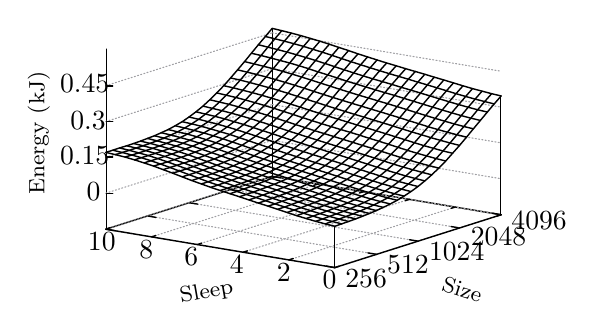
\begin{tikzpicture}[y=0.80pt, x=0.80pt, yscale=-0.570000, xscale=0.570000, inner sep=0pt, outer sep=0pt]
\begin{scope}[draw=black,line join=bevel,line cap=rect,even odd rule,line width=0.512pt]
  \begin{scope}[cm={{1.0,0.0,0.0,1.0,(0.0,0.0)}},draw=black,line join=bevel,line cap=rect,line width=0.512pt]
  \end{scope}
  \begin{scope}[cm={{1.00465,0.0,0.0,1.00465,(0.0,0.0)}},draw=black,line join=bevel,line cap=rect,line width=0.512pt]
  \end{scope}
  \begin{scope}[cm={{1.00465,0.0,0.0,1.00465,(0.0,0.0)}},draw=black,line join=round,line cap=round,line width=0.512pt]
    \path[draw] (59.1000,229.5000) -- (190.3000,187.8000);
    \path[draw] (370.9000,218.1000) -- (190.3000,187.8000);
    \path[draw] (59.5000,229.5000) -- (59.5000,87.5000);
    \path[draw] (190.5000,187.5000) -- (190.5000,71.5000);
    \path[draw] (370.5000,218.5000) -- (370.5000,124.5000);
  \end{scope}
  \begin{scope}[cm={{1.00465,0.0,0.0,1.00465,(0.0,0.0)}},draw=ca0a0a4,dash pattern=on 0.40pt off 0.80pt,line join=round,line cap=round,line width=0.400pt]
    \path[draw] (239.7000,259.8000) -- (59.1000,229.5000);
  \end{scope}
  \begin{scope}[cm={{1.00465,0.0,0.0,1.00465,(0.0,0.0)}},draw=black,line join=round,line cap=round,line width=0.512pt]
    \path[draw] (239.7000,259.8000) -- (232.9000,258.6000);
    \path[draw] (59.1000,229.5000) -- (65.8000,230.6000);
  \end{scope}
  \begin{scope}[cm={{1.00465,0.0,0.0,1.00465,(0.0,0.0)}},draw=black,line join=bevel,line cap=rect,line width=0.512pt]
  \end{scope}
  \begin{scope}[cm={{1.00465,0.0,0.0,1.00465,(249.153,276.781)}},draw=black,line join=bevel,line cap=rect,line width=0.512pt]
  \end{scope}
  \begin{scope}[cm={{1.00465,0.0,0.0,1.00465,(249.153,276.781)}},draw=black,line join=bevel,line cap=rect,line width=0.512pt]
  \end{scope}
  \begin{scope}[cm={{1.00465,0.0,0.0,1.00465,(249.153,276.781)}},draw=black,line join=bevel,line cap=rect,line width=0.512pt]
  \end{scope}
  \begin{scope}[cm={{1.00465,0.0,0.0,1.00465,(249.153,276.781)}},draw=black,line join=bevel,line cap=rect,line width=0.512pt]
  \end{scope}
  \begin{scope}[cm={{1.00465,0.0,0.0,1.00465,(249.153,276.781)}},draw=black,line join=bevel,line cap=rect,line width=0.512pt]
  \end{scope}
  \begin{scope}[cm={{1.00465,0.0,0.0,1.00465,(249.153,276.781)}},draw=black,line join=bevel,line cap=rect,line width=0.512pt]
    \path[fill=black] (0.0000,0.0000) node[above right] () {256};
  \end{scope}
  \begin{scope}[cm={{1.00465,0.0,0.0,1.00465,(249.153,276.781)}},draw=black,line join=bevel,line cap=rect,line width=0.512pt]
  \end{scope}
  \begin{scope}[cm={{1.00465,0.0,0.0,1.00465,(0.0,0.0)}},draw=black,line join=bevel,line cap=rect,line width=0.512pt]
  \end{scope}
  \begin{scope}[cm={{1.00465,0.0,0.0,1.00465,(0.0,0.0)}},draw=ca0a0a4,dash pattern=on 0.40pt off 0.80pt,line join=round,line cap=round,line width=0.400pt]
    \path[draw] (272.5000,249.3000) -- (91.9000,219.0000);
  \end{scope}
  \begin{scope}[cm={{1.00465,0.0,0.0,1.00465,(0.0,0.0)}},draw=black,line join=round,line cap=round,line width=0.512pt]
    \path[draw] (272.5000,249.3000) -- (265.8000,248.2000);
    \path[draw] (91.9000,219.0000) -- (98.6000,220.2000);
  \end{scope}
  \begin{scope}[cm={{1.00465,0.0,0.0,1.00465,(0.0,0.0)}},draw=black,line join=bevel,line cap=rect,line width=0.512pt]
  \end{scope}
  \begin{scope}[cm={{1.00465,0.0,0.0,1.00465,(282.307,265.73)}},draw=black,line join=bevel,line cap=rect,line width=0.512pt]
  \end{scope}
  \begin{scope}[cm={{1.00465,0.0,0.0,1.00465,(282.307,265.73)}},draw=black,line join=bevel,line cap=rect,line width=0.512pt]
  \end{scope}
  \begin{scope}[cm={{1.00465,0.0,0.0,1.00465,(282.307,265.73)}},draw=black,line join=bevel,line cap=rect,line width=0.512pt]
  \end{scope}
  \begin{scope}[cm={{1.00465,0.0,0.0,1.00465,(282.307,265.73)}},draw=black,line join=bevel,line cap=rect,line width=0.512pt]
  \end{scope}
  \begin{scope}[cm={{1.00465,0.0,0.0,1.00465,(282.307,265.73)}},draw=black,line join=bevel,line cap=rect,line width=0.512pt]
  \end{scope}
  \begin{scope}[cm={{1.00465,0.0,0.0,1.00465,(282.307,265.73)}},draw=black,line join=bevel,line cap=rect,line width=0.512pt]
    \path[fill=black] (0.0000,0.0000) node[above right] () {512};
  \end{scope}
  \begin{scope}[cm={{1.00465,0.0,0.0,1.00465,(282.307,265.73)}},draw=black,line join=bevel,line cap=rect,line width=0.512pt]
  \end{scope}
  \begin{scope}[cm={{1.00465,0.0,0.0,1.00465,(0.0,0.0)}},draw=black,line join=bevel,line cap=rect,line width=0.512pt]
  \end{scope}
  \begin{scope}[cm={{1.00465,0.0,0.0,1.00465,(0.0,0.0)}},draw=ca0a0a4,dash pattern=on 0.40pt off 0.80pt,line join=round,line cap=round,line width=0.400pt]
    \path[draw] (305.3000,238.9000) -- (124.7000,208.6000);
  \end{scope}
  \begin{scope}[cm={{1.00465,0.0,0.0,1.00465,(0.0,0.0)}},draw=black,line join=round,line cap=round,line width=0.512pt]
    \path[draw] (305.3000,238.9000) -- (298.6000,237.8000);
    \path[draw] (124.7000,208.6000) -- (131.4000,209.7000);
  \end{scope}
  \begin{scope}[cm={{1.00465,0.0,0.0,1.00465,(0.0,0.0)}},draw=black,line join=bevel,line cap=rect,line width=0.512pt]
  \end{scope}
  \begin{scope}[cm={{1.00465,0.0,0.0,1.00465,(315.46,255.684)}},draw=black,line join=bevel,line cap=rect,line width=0.512pt]
  \end{scope}
  \begin{scope}[cm={{1.00465,0.0,0.0,1.00465,(315.46,255.684)}},draw=black,line join=bevel,line cap=rect,line width=0.512pt]
  \end{scope}
  \begin{scope}[cm={{1.00465,0.0,0.0,1.00465,(315.46,255.684)}},draw=black,line join=bevel,line cap=rect,line width=0.512pt]
  \end{scope}
  \begin{scope}[cm={{1.00465,0.0,0.0,1.00465,(315.46,255.684)}},draw=black,line join=bevel,line cap=rect,line width=0.512pt]
  \end{scope}
  \begin{scope}[cm={{1.00465,0.0,0.0,1.00465,(315.46,255.684)}},draw=black,line join=bevel,line cap=rect,line width=0.512pt]
  \end{scope}
  \begin{scope}[cm={{1.00465,0.0,0.0,1.00465,(315.46,255.684)}},draw=black,line join=bevel,line cap=rect,line width=0.512pt]
    \path[fill=black] (0.0000,0.0000) node[above right] () {1024};
  \end{scope}
  \begin{scope}[cm={{1.00465,0.0,0.0,1.00465,(315.46,255.684)}},draw=black,line join=bevel,line cap=rect,line width=0.512pt]
  \end{scope}
  \begin{scope}[cm={{1.00465,0.0,0.0,1.00465,(0.0,0.0)}},draw=black,line join=bevel,line cap=rect,line width=0.512pt]
  \end{scope}
  \begin{scope}[cm={{1.00465,0.0,0.0,1.00465,(0.0,0.0)}},draw=ca0a0a4,dash pattern=on 0.40pt off 0.80pt,line join=round,line cap=round,line width=0.400pt]
    \path[draw] (338.1000,228.5000) -- (157.5000,198.2000);
  \end{scope}
  \begin{scope}[cm={{1.00465,0.0,0.0,1.00465,(0.0,0.0)}},draw=black,line join=round,line cap=round,line width=0.512pt]
    \path[draw] (338.1000,228.5000) -- (331.4000,227.4000);
    \path[draw] (157.5000,198.2000) -- (164.2000,199.3000);
  \end{scope}
  \begin{scope}[cm={{1.00465,0.0,0.0,1.00465,(0.0,0.0)}},draw=black,line join=bevel,line cap=rect,line width=0.512pt]
  \end{scope}
  \begin{scope}[cm={{1.00465,0.0,0.0,1.00465,(348.614,244.633)}},draw=black,line join=bevel,line cap=rect,line width=0.512pt]
  \end{scope}
  \begin{scope}[cm={{1.00465,0.0,0.0,1.00465,(348.614,244.633)}},draw=black,line join=bevel,line cap=rect,line width=0.512pt]
  \end{scope}
  \begin{scope}[cm={{1.00465,0.0,0.0,1.00465,(348.614,244.633)}},draw=black,line join=bevel,line cap=rect,line width=0.512pt]
  \end{scope}
  \begin{scope}[cm={{1.00465,0.0,0.0,1.00465,(348.614,244.633)}},draw=black,line join=bevel,line cap=rect,line width=0.512pt]
  \end{scope}
  \begin{scope}[cm={{1.00465,0.0,0.0,1.00465,(348.614,244.633)}},draw=black,line join=bevel,line cap=rect,line width=0.512pt]
  \end{scope}
  \begin{scope}[cm={{1.00465,0.0,0.0,1.00465,(348.614,243.133)}},draw=black,line join=bevel,line cap=rect,line width=0.512pt]
    \path[fill=black] (0.0000,0.0000) node[above right] () {2048};
  \end{scope}
  \begin{scope}[cm={{1.00465,0.0,0.0,1.00465,(348.614,244.633)}},draw=black,line join=bevel,line cap=rect,line width=0.512pt]
  \end{scope}
  \begin{scope}[cm={{1.00465,0.0,0.0,1.00465,(0.0,0.0)}},draw=black,line join=bevel,line cap=rect,line width=0.512pt]
  \end{scope}
  \begin{scope}[cm={{1.00465,0.0,0.0,1.00465,(0.0,0.0)}},draw=ca0a0a4,dash pattern=on 0.40pt off 0.80pt,line join=round,line cap=round,line width=0.400pt]
    \path[draw] (370.9000,218.1000) -- (190.3000,187.8000);
  \end{scope}
  \begin{scope}[cm={{1.00465,0.0,0.0,1.00465,(0.0,0.0)}},draw=black,line join=round,line cap=round,line width=0.512pt]
    \path[draw] (370.9000,218.1000) -- (364.2000,216.9000);
    \path[draw] (190.3000,187.8000) -- (197.1000,188.9000);
  \end{scope}
  \begin{scope}[cm={{1.00465,0.0,0.0,1.00465,(0.0,0.0)}},draw=black,line join=bevel,line cap=rect,line width=0.512pt]
  \end{scope}
  \begin{scope}[cm={{1.00465,0.0,0.0,1.00465,(380.763,234.586)}},draw=black,line join=bevel,line cap=rect,line width=0.512pt]
  \end{scope}
  \begin{scope}[cm={{1.00465,0.0,0.0,1.00465,(380.763,234.586)}},draw=black,line join=bevel,line cap=rect,line width=0.512pt]
  \end{scope}
  \begin{scope}[cm={{1.00465,0.0,0.0,1.00465,(380.763,234.586)}},draw=black,line join=bevel,line cap=rect,line width=0.512pt]
  \end{scope}
  \begin{scope}[cm={{1.00465,0.0,0.0,1.00465,(380.763,234.586)}},draw=black,line join=bevel,line cap=rect,line width=0.512pt]
  \end{scope}
  \begin{scope}[cm={{1.00465,0.0,0.0,1.00465,(380.763,234.586)}},draw=black,line join=bevel,line cap=rect,line width=0.512pt]
  \end{scope}
  \begin{scope}[cm={{1.00465,0.0,0.0,1.00465,(380.763,230.586)}},draw=black,line join=bevel,line cap=rect,line width=0.512pt]
    \path[fill=black] (0.0000,0.0000) node[above right] () {4096};
  \end{scope}
  \begin{scope}[cm={{1.00465,0.0,0.0,1.00465,(380.763,234.586)}},draw=black,line join=bevel,line cap=rect,line width=0.512pt]
  \end{scope}
  \begin{scope}[cm={{1.00465,0.0,0.0,1.00465,(0.0,0.0)}},draw=black,line join=bevel,line cap=rect,line width=0.512pt]
  \end{scope}
  \begin{scope}[cm={{1.00465,0.0,0.0,1.00465,(0.0,0.0)}},draw=ca0a0a4,dash pattern=on 0.40pt off 0.80pt,line join=round,line cap=round,line width=0.400pt]
    \path[draw] (239.7000,259.8000) -- (370.9000,218.1000);
  \end{scope}
  \begin{scope}[cm={{1.00465,0.0,0.0,1.00465,(0.0,0.0)}},draw=black,line join=round,line cap=round,line width=0.512pt]
    \path[draw] (239.7000,259.8000) -- (242.9000,258.7000);
    \path[draw] (370.9000,218.1000) -- (367.6000,219.1000);
  \end{scope}
  \begin{scope}[cm={{1.00465,0.0,0.0,1.00465,(0.0,0.0)}},draw=black,line join=bevel,line cap=rect,line width=0.512pt]
  \end{scope}
  \begin{scope}[cm={{1.00465,0.0,0.0,1.00465,(231.07,275.777)}},draw=black,line join=bevel,line cap=rect,line width=0.512pt]
  \end{scope}
  \begin{scope}[cm={{1.00465,0.0,0.0,1.00465,(231.07,275.777)}},draw=black,line join=bevel,line cap=rect,line width=0.512pt]
  \end{scope}
  \begin{scope}[cm={{1.00465,0.0,0.0,1.00465,(231.07,275.777)}},draw=black,line join=bevel,line cap=rect,line width=0.512pt]
  \end{scope}
  \begin{scope}[cm={{1.00465,0.0,0.0,1.00465,(231.07,275.777)}},draw=black,line join=bevel,line cap=rect,line width=0.512pt]
  \end{scope}
  \begin{scope}[cm={{1.00465,0.0,0.0,1.00465,(231.07,275.777)}},draw=black,line join=bevel,line cap=rect,line width=0.512pt]
  \end{scope}
  \begin{scope}[cm={{1.00465,0.0,0.0,1.00465,(231.07,277.777)}},draw=black,line join=bevel,line cap=rect,line width=0.512pt]
    \path[fill=black] (0.0000,0.0000) node[above right] () {0};
  \end{scope}
  \begin{scope}[cm={{1.00465,0.0,0.0,1.00465,(231.07,275.777)}},draw=black,line join=bevel,line cap=rect,line width=0.512pt]
  \end{scope}
  \begin{scope}[cm={{1.00465,0.0,0.0,1.00465,(0.0,0.0)}},draw=black,line join=bevel,line cap=rect,line width=0.512pt]
  \end{scope}
  \begin{scope}[cm={{1.00465,0.0,0.0,1.00465,(0.0,0.0)}},draw=ca0a0a4,dash pattern=on 0.40pt off 0.80pt,line join=round,line cap=round,line width=0.400pt]
    \path[draw] (203.6000,253.7000) -- (334.8000,212.0000);
  \end{scope}
  \begin{scope}[cm={{1.00465,0.0,0.0,1.00465,(0.0,0.0)}},draw=black,line join=round,line cap=round,line width=0.512pt]
    \path[draw] (203.6000,253.7000) -- (206.9000,252.6000);
    \path[draw] (334.8000,212.0000) -- (331.5000,213.0000);
  \end{scope}
  \begin{scope}[cm={{1.00465,0.0,0.0,1.00465,(0.0,0.0)}},draw=black,line join=bevel,line cap=rect,line width=0.512pt]
  \end{scope}
  \begin{scope}[cm={{1.00465,0.0,0.0,1.00465,(194.902,269.749)}},draw=black,line join=bevel,line cap=rect,line width=0.512pt]
  \end{scope}
  \begin{scope}[cm={{1.00465,0.0,0.0,1.00465,(194.902,269.749)}},draw=black,line join=bevel,line cap=rect,line width=0.512pt]
  \end{scope}
  \begin{scope}[cm={{1.00465,0.0,0.0,1.00465,(194.902,269.749)}},draw=black,line join=bevel,line cap=rect,line width=0.512pt]
  \end{scope}
  \begin{scope}[cm={{1.00465,0.0,0.0,1.00465,(194.902,269.749)}},draw=black,line join=bevel,line cap=rect,line width=0.512pt]
  \end{scope}
  \begin{scope}[cm={{1.00465,0.0,0.0,1.00465,(194.902,269.749)}},draw=black,line join=bevel,line cap=rect,line width=0.512pt]
  \end{scope}
  \begin{scope}[cm={{1.00465,0.0,0.0,1.00465,(194.902,271.749)}},draw=black,line join=bevel,line cap=rect,line width=0.512pt]
    \path[fill=black] (0.0000,0.0000) node[above right] () {2};
  \end{scope}
  \begin{scope}[cm={{1.00465,0.0,0.0,1.00465,(194.902,269.749)}},draw=black,line join=bevel,line cap=rect,line width=0.512pt]
  \end{scope}
  \begin{scope}[cm={{1.00465,0.0,0.0,1.00465,(0.0,0.0)}},draw=black,line join=bevel,line cap=rect,line width=0.512pt]
  \end{scope}
  \begin{scope}[cm={{1.00465,0.0,0.0,1.00465,(0.0,0.0)}},draw=ca0a0a4,dash pattern=on 0.40pt off 0.80pt,line join=round,line cap=round,line width=0.400pt]
    \path[draw] (167.5000,247.6000) -- (298.6000,205.9000);
  \end{scope}
  \begin{scope}[cm={{1.00465,0.0,0.0,1.00465,(0.0,0.0)}},draw=black,line join=round,line cap=round,line width=0.512pt]
    \path[draw] (167.5000,247.6000) -- (170.8000,246.6000);
    \path[draw] (298.6000,205.9000) -- (295.3000,207.0000);
  \end{scope}
  \begin{scope}[cm={{1.00465,0.0,0.0,1.00465,(0.0,0.0)}},draw=black,line join=bevel,line cap=rect,line width=0.512pt]
  \end{scope}
  \begin{scope}[cm={{1.00465,0.0,0.0,1.00465,(157.73,263.721)}},draw=black,line join=bevel,line cap=rect,line width=0.512pt]
  \end{scope}
  \begin{scope}[cm={{1.00465,0.0,0.0,1.00465,(157.73,263.721)}},draw=black,line join=bevel,line cap=rect,line width=0.512pt]
  \end{scope}
  \begin{scope}[cm={{1.00465,0.0,0.0,1.00465,(157.73,263.721)}},draw=black,line join=bevel,line cap=rect,line width=0.512pt]
  \end{scope}
  \begin{scope}[cm={{1.00465,0.0,0.0,1.00465,(157.73,263.721)}},draw=black,line join=bevel,line cap=rect,line width=0.512pt]
  \end{scope}
  \begin{scope}[cm={{1.00465,0.0,0.0,1.00465,(157.73,263.721)}},draw=black,line join=bevel,line cap=rect,line width=0.512pt]
  \end{scope}
  \begin{scope}[cm={{1.00465,0.0,0.0,1.00465,(157.73,265.721)}},draw=black,line join=bevel,line cap=rect,line width=0.512pt]
    \path[fill=black] (0.0000,0.0000) node[above right] () {4};
  \end{scope}
  \begin{scope}[cm={{1.00465,0.0,0.0,1.00465,(157.73,263.721)}},draw=black,line join=bevel,line cap=rect,line width=0.512pt]
  \end{scope}
  \begin{scope}[cm={{1.00465,0.0,0.0,1.00465,(0.0,0.0)}},draw=black,line join=bevel,line cap=rect,line width=0.512pt]
  \end{scope}
  \begin{scope}[cm={{1.00465,0.0,0.0,1.00465,(0.0,0.0)}},draw=ca0a0a4,dash pattern=on 0.40pt off 0.80pt,line join=round,line cap=round,line width=0.400pt]
    \path[draw] (131.4000,241.6000) -- (262.5000,199.9000);
  \end{scope}
  \begin{scope}[cm={{1.00465,0.0,0.0,1.00465,(0.0,0.0)}},draw=black,line join=round,line cap=round,line width=0.512pt]
    \path[draw] (131.4000,241.6000) -- (134.7000,240.5000);
    \path[draw] (262.5000,199.9000) -- (259.2000,200.9000);
  \end{scope}
  \begin{scope}[cm={{1.00465,0.0,0.0,1.00465,(0.0,0.0)}},draw=black,line join=bevel,line cap=rect,line width=0.512pt]
  \end{scope}
  \begin{scope}[cm={{1.00465,0.0,0.0,1.00465,(121.563,257.693)}},draw=black,line join=bevel,line cap=rect,line width=0.512pt]
  \end{scope}
  \begin{scope}[cm={{1.00465,0.0,0.0,1.00465,(121.563,257.693)}},draw=black,line join=bevel,line cap=rect,line width=0.512pt]
  \end{scope}
  \begin{scope}[cm={{1.00465,0.0,0.0,1.00465,(121.563,257.693)}},draw=black,line join=bevel,line cap=rect,line width=0.512pt]
  \end{scope}
  \begin{scope}[cm={{1.00465,0.0,0.0,1.00465,(121.563,257.693)}},draw=black,line join=bevel,line cap=rect,line width=0.512pt]
  \end{scope}
  \begin{scope}[cm={{1.00465,0.0,0.0,1.00465,(121.563,257.693)}},draw=black,line join=bevel,line cap=rect,line width=0.512pt]
  \end{scope}
  \begin{scope}[cm={{1.00465,0.0,0.0,1.00465,(121.563,259.693)}},draw=black,line join=bevel,line cap=rect,line width=0.512pt]
    \path[fill=black] (0.0000,0.0000) node[above right] () {6};
  \end{scope}
  \begin{scope}[cm={{1.00465,0.0,0.0,1.00465,(121.563,257.693)}},draw=black,line join=bevel,line cap=rect,line width=0.512pt]
  \end{scope}
  \begin{scope}[cm={{1.00465,0.0,0.0,1.00465,(0.0,0.0)}},draw=black,line join=bevel,line cap=rect,line width=0.512pt]
  \end{scope}
  \begin{scope}[cm={{1.00465,0.0,0.0,1.00465,(0.0,0.0)}},draw=ca0a0a4,dash pattern=on 0.40pt off 0.80pt,line join=round,line cap=round,line width=0.400pt]
    \path[draw] (95.2000,235.5000) -- (226.4000,193.8000);
  \end{scope}
  \begin{scope}[cm={{1.00465,0.0,0.0,1.00465,(0.0,0.0)}},draw=black,line join=round,line cap=round,line width=0.512pt]
    \path[draw] (95.2000,235.5000) -- (98.5000,234.5000);
    \path[draw] (226.4000,193.8000) -- (223.1000,194.9000);
  \end{scope}
  \begin{scope}[cm={{1.00465,0.0,0.0,1.00465,(0.0,0.0)}},draw=black,line join=bevel,line cap=rect,line width=0.512pt]
  \end{scope}
  \begin{scope}[cm={{1.00465,0.0,0.0,1.00465,(85.8977,251.665)}},draw=black,line join=bevel,line cap=rect,line width=0.512pt]
  \end{scope}
  \begin{scope}[cm={{1.00465,0.0,0.0,1.00465,(85.8977,251.665)}},draw=black,line join=bevel,line cap=rect,line width=0.512pt]
  \end{scope}
  \begin{scope}[cm={{1.00465,0.0,0.0,1.00465,(85.8977,251.665)}},draw=black,line join=bevel,line cap=rect,line width=0.512pt]
  \end{scope}
  \begin{scope}[cm={{1.00465,0.0,0.0,1.00465,(85.8977,251.665)}},draw=black,line join=bevel,line cap=rect,line width=0.512pt]
  \end{scope}
  \begin{scope}[cm={{1.00465,0.0,0.0,1.00465,(85.8977,251.665)}},draw=black,line join=bevel,line cap=rect,line width=0.512pt]
  \end{scope}
  \begin{scope}[cm={{1.00465,0.0,0.0,1.00465,(85.8977,253.665)}},draw=black,line join=bevel,line cap=rect,line width=0.512pt]
    \path[fill=black] (0.0000,0.0000) node[above right] () {8};
  \end{scope}
  \begin{scope}[cm={{1.00465,0.0,0.0,1.00465,(85.8977,251.665)}},draw=black,line join=bevel,line cap=rect,line width=0.512pt]
  \end{scope}
  \begin{scope}[cm={{1.00465,0.0,0.0,1.00465,(0.0,0.0)}},draw=black,line join=bevel,line cap=rect,line width=0.512pt]
  \end{scope}
  \begin{scope}[cm={{1.00465,0.0,0.0,1.00465,(0.0,0.0)}},draw=ca0a0a4,dash pattern=on 0.40pt off 0.80pt,line join=round,line cap=round,line width=0.400pt]
    \path[draw] (59.1000,229.5000) -- (190.3000,187.8000);
  \end{scope}
  \begin{scope}[cm={{1.00465,0.0,0.0,1.00465,(0.0,0.0)}},draw=black,line join=round,line cap=round,line width=0.512pt]
    \path[draw] (59.1000,229.5000) -- (62.4000,228.4000);
    \path[draw] (190.3000,187.8000) -- (187.1000,188.8000);
  \end{scope}
  \begin{scope}[cm={{1.00465,0.0,0.0,1.00465,(0.0,0.0)}},draw=black,line join=bevel,line cap=rect,line width=0.512pt]
  \end{scope}
  \begin{scope}[cm={{1.00465,0.0,0.0,1.00465,(45.2093,245.637)}},draw=black,line join=bevel,line cap=rect,line width=0.512pt]
  \end{scope}
  \begin{scope}[cm={{1.00465,0.0,0.0,1.00465,(45.2093,245.637)}},draw=black,line join=bevel,line cap=rect,line width=0.512pt]
  \end{scope}
  \begin{scope}[cm={{1.00465,0.0,0.0,1.00465,(45.2093,245.637)}},draw=black,line join=bevel,line cap=rect,line width=0.512pt]
  \end{scope}
  \begin{scope}[cm={{1.00465,0.0,0.0,1.00465,(45.2093,245.637)}},draw=black,line join=bevel,line cap=rect,line width=0.512pt]
  \end{scope}
  \begin{scope}[cm={{1.00465,0.0,0.0,1.00465,(45.2093,245.637)}},draw=black,line join=bevel,line cap=rect,line width=0.512pt]
  \end{scope}
  \begin{scope}[cm={{1.00465,0.0,0.0,1.00465,(45.2093,247.637)}},draw=black,line join=bevel,line cap=rect,line width=0.512pt]
    \path[fill=black] (0.0000,0.0000) node[above right] () {10};
  \end{scope}
  \begin{scope}[cm={{1.00465,0.0,0.0,1.00465,(45.2093,245.637)}},draw=black,line join=bevel,line cap=rect,line width=0.512pt]
  \end{scope}
  \begin{scope}[cm={{1.00465,0.0,0.0,1.00465,(0.0,0.0)}},draw=black,line join=bevel,line cap=rect,line width=0.512pt]
  \end{scope}
  \begin{scope}[cm={{1.00465,0.0,0.0,1.00465,(0.0,0.0)}},draw=ca0a0a4,dash pattern=on 0.40pt off 0.80pt,line join=round,line cap=round,line width=0.400pt]
    \path[draw] (59.1000,201.1000) -- (190.3000,159.4000);
    \path[draw] (190.3000,159.4000) -- (190.3000,159.4000) -- (370.9000,189.7000);
  \end{scope}
  \begin{scope}[cm={{1.00465,0.0,0.0,1.00465,(0.0,0.0)}},draw=black,line join=round,line cap=round,line width=0.512pt]
    \path[draw] (59.5000,201.5000) -- (64.5000,201.5000);
  \end{scope}
  \begin{scope}[cm={{1.00465,0.0,0.0,1.00465,(0.0,0.0)}},draw=black,line join=bevel,line cap=rect,line width=0.512pt]
  \end{scope}
  \begin{scope}[cm={{1.00465,0.0,0.0,1.00465,(40.186,207.46)}},draw=black,line join=bevel,line cap=rect,line width=0.512pt]
  \end{scope}
  \begin{scope}[cm={{1.00465,0.0,0.0,1.00465,(40.186,207.46)}},draw=black,line join=bevel,line cap=rect,line width=0.512pt]
  \end{scope}
  \begin{scope}[cm={{1.00465,0.0,0.0,1.00465,(40.186,207.46)}},draw=black,line join=bevel,line cap=rect,line width=0.512pt]
  \end{scope}
  \begin{scope}[cm={{1.00465,0.0,0.0,1.00465,(40.186,207.46)}},draw=black,line join=bevel,line cap=rect,line width=0.512pt]
  \end{scope}
  \begin{scope}[cm={{1.00465,0.0,0.0,1.00465,(40.186,207.46)}},draw=black,line join=bevel,line cap=rect,line width=0.512pt]
  \end{scope}
  \begin{scope}[cm={{1.00465,0.0,0.0,1.00465,(44.186,207.46)}},draw=black,line join=bevel,line cap=rect,line width=0.512pt]
    \path[fill=black] (0.0000,0.0000) node[above right] () {0};
  \end{scope}
  \begin{scope}[cm={{1.00465,0.0,0.0,1.00465,(40.186,207.46)}},draw=black,line join=bevel,line cap=rect,line width=0.512pt]
  \end{scope}
  \begin{scope}[cm={{1.00465,0.0,0.0,1.00465,(0.0,0.0)}},draw=black,line join=bevel,line cap=rect,line width=0.512pt]
  \end{scope}
  \begin{scope}[cm={{1.00465,0.0,0.0,1.00465,(0.0,0.0)}},draw=ca0a0a4,dash pattern=on 0.40pt off 0.80pt,line join=round,line cap=round,line width=0.400pt]
    \path[draw] (59.1000,172.8000) -- (190.3000,131.2000);
    \path[draw] (190.3000,131.2000) -- (190.3000,131.2000) -- (370.9000,161.4000);
  \end{scope}
  \begin{scope}[cm={{1.00465,0.0,0.0,1.00465,(0.0,0.0)}},draw=black,line join=round,line cap=round,line width=0.512pt]
    \path[draw] (59.5000,172.5000) -- (64.5000,172.5000);
  \end{scope}
  \begin{scope}[cm={{1.00465,0.0,0.0,1.00465,(0.0,0.0)}},draw=black,line join=bevel,line cap=rect,line width=0.512pt]
  \end{scope}
  \begin{scope}[cm={{1.00465,0.0,0.0,1.00465,(29.1349,179.33)}},draw=black,line join=bevel,line cap=rect,line width=0.512pt]
  \end{scope}
  \begin{scope}[cm={{1.00465,0.0,0.0,1.00465,(29.1349,179.33)}},draw=black,line join=bevel,line cap=rect,line width=0.512pt]
  \end{scope}
  \begin{scope}[cm={{1.00465,0.0,0.0,1.00465,(29.1349,179.33)}},draw=black,line join=bevel,line cap=rect,line width=0.512pt]
  \end{scope}
  \begin{scope}[cm={{1.00465,0.0,0.0,1.00465,(29.1349,179.33)}},draw=black,line join=bevel,line cap=rect,line width=0.512pt]
  \end{scope}
  \begin{scope}[cm={{1.00465,0.0,0.0,1.00465,(29.1349,179.33)}},draw=black,line join=bevel,line cap=rect,line width=0.512pt]
  \end{scope}
  \begin{scope}[cm={{1.00465,0.0,0.0,1.00465,(23.1349,179.33)}},draw=black,line join=bevel,line cap=rect,line width=0.512pt]
    \path[fill=black] (0.0000,0.0000) node[above right] () {0.15};
  \end{scope}
  \begin{scope}[cm={{1.00465,0.0,0.0,1.00465,(29.1349,179.33)}},draw=black,line join=bevel,line cap=rect,line width=0.512pt]
  \end{scope}
  \begin{scope}[cm={{1.00465,0.0,0.0,1.00465,(0.0,0.0)}},draw=black,line join=bevel,line cap=rect,line width=0.512pt]
  \end{scope}
  \begin{scope}[cm={{1.00465,0.0,0.0,1.00465,(0.0,0.0)}},draw=ca0a0a4,dash pattern=on 0.40pt off 0.80pt,line join=round,line cap=round,line width=0.400pt]
    \path[draw] (59.1000,144.6000) -- (190.3000,102.9000);
    \path[draw] (190.3000,102.9000) -- (190.3000,102.9000) -- (370.9000,133.2000);
  \end{scope}
  \begin{scope}[cm={{1.00465,0.0,0.0,1.00465,(0.0,0.0)}},draw=black,line join=round,line cap=round,line width=0.512pt]
    \path[draw] (59.5000,144.5000) -- (64.5000,144.5000);
  \end{scope}
  \begin{scope}[cm={{1.00465,0.0,0.0,1.00465,(0.0,0.0)}},draw=black,line join=bevel,line cap=rect,line width=0.512pt]
  \end{scope}
  \begin{scope}[cm={{1.00465,0.0,0.0,1.00465,(41.1907,151.2)}},draw=black,line join=bevel,line cap=rect,line width=0.512pt]
  \end{scope}
  \begin{scope}[cm={{1.00465,0.0,0.0,1.00465,(41.1907,151.2)}},draw=black,line join=bevel,line cap=rect,line width=0.512pt]
  \end{scope}
  \begin{scope}[cm={{1.00465,0.0,0.0,1.00465,(41.1907,151.2)}},draw=black,line join=bevel,line cap=rect,line width=0.512pt]
  \end{scope}
  \begin{scope}[cm={{1.00465,0.0,0.0,1.00465,(41.1907,151.2)}},draw=black,line join=bevel,line cap=rect,line width=0.512pt]
  \end{scope}
  \begin{scope}[cm={{1.00465,0.0,0.0,1.00465,(41.1907,151.2)}},draw=black,line join=bevel,line cap=rect,line width=0.512pt]
  \end{scope}
  \begin{scope}[cm={{1.00465,0.0,0.0,1.00465,(31.1907,151.2)}},draw=black,line join=bevel,line cap=rect,line width=0.512pt]
    \path[fill=black] (0.0000,0.0000) node[above right] () {0.3};
  \end{scope}
  \begin{scope}[cm={{1.00465,0.0,0.0,1.00465,(41.1907,151.2)}},draw=black,line join=bevel,line cap=rect,line width=0.512pt]
  \end{scope}
  \begin{scope}[cm={{1.00465,0.0,0.0,1.00465,(0.0,0.0)}},draw=black,line join=bevel,line cap=rect,line width=0.512pt]
  \end{scope}
  \begin{scope}[cm={{1.00465,0.0,0.0,1.00465,(0.0,0.0)}},draw=ca0a0a4,dash pattern=on 0.40pt off 0.80pt,line join=round,line cap=round,line width=0.400pt]
    \path[draw] (59.1000,116.3000) -- (190.3000,74.6000);
    \path[draw] (190.3000,74.6000) -- (190.3000,74.6000) -- (370.9000,104.9000);
  \end{scope}
  \begin{scope}[cm={{1.00465,0.0,0.0,1.00465,(0.0,0.0)}},draw=black,line join=round,line cap=round,line width=0.512pt]
    \path[draw] (59.5000,116.5000) -- (64.5000,116.5000);
  \end{scope}
  \begin{scope}[cm={{1.00465,0.0,0.0,1.00465,(0.0,0.0)}},draw=black,line join=bevel,line cap=rect,line width=0.512pt]
  \end{scope}
  \begin{scope}[cm={{1.00465,0.0,0.0,1.00465,(29.1349,122.065)}},draw=black,line join=bevel,line cap=rect,line width=0.512pt]
  \end{scope}
  \begin{scope}[cm={{1.00465,0.0,0.0,1.00465,(29.1349,122.065)}},draw=black,line join=bevel,line cap=rect,line width=0.512pt]
  \end{scope}
  \begin{scope}[cm={{1.00465,0.0,0.0,1.00465,(29.1349,122.065)}},draw=black,line join=bevel,line cap=rect,line width=0.512pt]
  \end{scope}
  \begin{scope}[cm={{1.00465,0.0,0.0,1.00465,(29.1349,122.065)}},draw=black,line join=bevel,line cap=rect,line width=0.512pt]
  \end{scope}
  \begin{scope}[cm={{1.00465,0.0,0.0,1.00465,(29.1349,122.065)}},draw=black,line join=bevel,line cap=rect,line width=0.512pt]
  \end{scope}
  \begin{scope}[cm={{1.00465,0.0,0.0,1.00465,(23.1349,122.065)}},draw=black,line join=bevel,line cap=rect,line width=0.512pt]
    \path[fill=black] (0.0000,0.0000) node[above right] () {0.45};
  \end{scope}
  \begin{scope}[cm={{1.00465,0.0,0.0,1.00465,(29.1349,122.065)}},draw=black,line join=bevel,line cap=rect,line width=0.512pt]
  \end{scope}
  \begin{scope}[cm={{0.0,-1.00465,1.00465,0.0,(15.5721,196.409)}},draw=black,line join=bevel,line cap=rect,line width=0.512pt]
  \end{scope}
  \begin{scope}[cm={{0.0,-1.00465,1.00465,0.0,(15.5721,196.409)}},draw=black,line join=bevel,line cap=rect,line width=0.512pt]
  \end{scope}
  \begin{scope}[cm={{0.0,-1.00465,1.00465,0.0,(15.5721,196.409)}},draw=black,line join=bevel,line cap=rect,line width=0.512pt]
  \end{scope}
  \begin{scope}[cm={{0.0,-1.00465,1.00465,0.0,(15.5721,196.409)}},draw=black,line join=bevel,line cap=rect,line width=0.512pt]
  \end{scope}
  \begin{scope}[cm={{0.0,-1.00465,1.00465,0.0,(15.5721,196.409)}},draw=black,line join=bevel,line cap=rect,line width=0.512pt]
  \end{scope}
  \begin{scope}[cm={{0.0,-1.00465,1.00465,0.0,(-2.5721,203.298)}},draw=black,line join=bevel,line cap=rect,line width=0.512pt]
    \path[fill=black] (0.0000,0.0000) node[above right] () {\rotatebox{90}{\footnotesize Energy (kJ)}};
  \end{scope}
  \begin{scope}[cm={{0.0,-1.00465,1.00465,0.0,(15.5721,196.409)}},draw=black,line join=bevel,line cap=rect,line width=0.512pt]
  \end{scope}
  \begin{scope}[cm={{1.00465,0.0,0.0,1.00465,(0.0,0.0)}},draw=black,line join=bevel,line cap=rect,line width=0.512pt]
  \end{scope}
  \begin{scope}[cm={{1.00465,0.0,0.0,1.00465,(0.0,0.0)}},draw=black,line join=bevel,line cap=rect,line width=0.512pt]
  \end{scope}
  \begin{scope}[cm={{1.00465,0.0,0.0,1.00465,(0.0,0.0)}},draw=black,line join=bevel,line cap=rect,line width=0.512pt]
  \end{scope}
  \begin{scope}[cm={{1.00465,0.0,0.0,1.00465,(0.0,0.0)}},draw=black,line join=round,line cap=round,line width=0.512pt]
    \path[draw] (370.9000,124.4000) -- (363.4000,122.6000) -- (363.4000,122.6000) --
      (355.8000,120.6000) -- (355.8000,120.6000) -- (348.3000,118.6000) --
      (348.3000,118.6000) -- (340.8000,116.4000) -- (340.8000,116.4000) --
      (333.3000,114.1000) -- (333.3000,114.1000) -- (325.7000,111.8000) --
      (325.7000,111.8000) -- (318.2000,109.6000) -- (318.2000,109.6000) --
      (310.7000,107.3000) -- (310.7000,107.3000) -- (303.2000,105.1000) --
      (303.2000,105.1000) -- (295.6000,102.9000) -- (295.6000,102.9000) --
      (288.1000,100.6000) -- (288.1000,100.6000) -- (280.6000,98.4000) --
      (280.6000,98.4000) -- (273.0000,96.0000) -- (273.0000,96.0000) --
      (265.5000,93.6000) -- (265.5000,93.6000) -- (258.0000,91.2000) --
      (258.0000,91.2000) -- (250.5000,88.6000) -- (250.5000,88.6000) --
      (242.9000,86.1000) -- (242.9000,86.1000) -- (235.4000,83.6000) --
      (235.4000,83.6000) -- (227.9000,81.2000) -- (227.9000,81.2000) --
      (220.4000,79.0000) -- (220.4000,79.0000) -- (212.9000,76.8000) --
      (212.9000,76.8000) -- (205.4000,74.8000) -- (205.4000,74.8000) --
      (197.9000,72.9000) -- (197.9000,72.9000) -- (190.3000,71.1000);
    \path[draw] (365.4000,130.7000) -- (357.9000,128.8000) -- (357.9000,128.8000) --
      (350.4000,126.9000) -- (350.4000,126.9000) -- (342.9000,124.8000) --
      (342.9000,124.8000) -- (335.3000,122.6000) -- (335.3000,122.6000) --
      (327.8000,120.3000) -- (327.8000,120.3000) -- (320.3000,118.0000) --
      (320.3000,118.0000) -- (312.7000,115.7000) -- (312.7000,115.7000) --
      (305.2000,113.5000) -- (305.2000,113.5000) -- (297.7000,111.2000) --
      (297.7000,111.2000) -- (290.2000,109.0000) -- (290.2000,109.0000) --
      (282.6000,106.8000) -- (282.6000,106.8000) -- (275.1000,104.5000) --
      (275.1000,104.5000) -- (267.6000,102.2000) -- (267.6000,102.2000) --
      (260.1000,99.8000) -- (260.1000,99.8000) -- (252.5000,97.4000) --
      (252.5000,97.4000) -- (245.0000,94.9000) -- (245.0000,94.9000) --
      (237.5000,92.4000) -- (237.5000,92.4000) -- (229.9000,89.9000) --
      (229.9000,89.9000) -- (222.4000,87.6000) -- (222.4000,87.6000) --
      (215.0000,85.3000) -- (215.0000,85.3000) -- (207.5000,83.2000) --
      (207.5000,83.2000) -- (199.9000,81.2000) -- (199.9000,81.2000) --
      (192.4000,79.3000) -- (192.4000,79.3000) -- (184.9000,77.5000);
    \path[draw] (360.0000,137.1000) -- (352.4000,135.3000) -- (352.4000,135.3000) --
      (344.9000,133.3000) -- (344.9000,133.3000) -- (337.4000,131.2000) --
      (337.4000,131.2000) -- (329.9000,129.0000) -- (329.9000,129.0000) --
      (322.3000,126.7000) -- (322.3000,126.7000) -- (314.8000,124.4000) --
      (314.8000,124.4000) -- (307.3000,122.1000) -- (307.3000,122.1000) --
      (299.7000,119.8000) -- (299.7000,119.8000) -- (292.2000,117.6000) --
      (292.2000,117.6000) -- (284.7000,115.3000) -- (284.7000,115.3000) --
      (277.2000,113.1000) -- (277.2000,113.1000) -- (269.6000,110.9000) --
      (269.6000,110.9000) -- (262.1000,108.6000) -- (262.1000,108.6000) --
      (254.6000,106.2000) -- (254.6000,106.2000) -- (247.1000,103.8000) --
      (247.1000,103.8000) -- (239.5000,101.3000) -- (239.5000,101.3000) --
      (232.0000,98.8000) -- (232.0000,98.8000) -- (224.5000,96.4000) --
      (224.5000,96.4000) -- (216.9000,94.1000) -- (216.9000,94.1000) --
      (209.5000,91.9000) -- (209.5000,91.9000) -- (202.0000,89.8000) --
      (202.0000,89.8000) -- (194.5000,87.8000) -- (194.5000,87.8000) --
      (186.9000,85.9000) -- (186.9000,85.9000) -- (179.4000,84.0000);
    \path[draw] (354.5000,143.7000) -- (347.0000,141.9000) -- (347.0000,141.9000) --
      (339.4000,139.9000) -- (339.4000,139.9000) -- (331.9000,137.7000) --
      (331.9000,137.7000) -- (324.4000,135.5000) -- (324.4000,135.5000) --
      (316.9000,133.2000) -- (316.9000,133.2000) -- (309.3000,130.9000) --
      (309.3000,130.9000) -- (301.8000,128.6000) -- (301.8000,128.6000) --
      (294.3000,126.3000) -- (294.3000,126.3000) -- (286.8000,124.0000) --
      (286.8000,124.0000) -- (279.2000,121.8000) -- (279.2000,121.8000) --
      (271.7000,119.6000) -- (271.7000,119.6000) -- (264.2000,117.3000) --
      (264.2000,117.3000) -- (256.6000,115.0000) -- (256.6000,115.0000) --
      (249.1000,112.7000) -- (249.1000,112.7000) -- (241.6000,110.2000) --
      (241.6000,110.2000) -- (234.1000,107.8000) -- (234.1000,107.8000) --
      (226.5000,105.4000) -- (226.5000,105.4000) -- (219.0000,102.9000) --
      (219.0000,102.9000) -- (211.6000,100.6000) -- (211.6000,100.6000) --
      (204.1000,98.4000) -- (204.1000,98.4000) -- (196.5000,96.4000) --
      (196.5000,96.4000) -- (189.0000,94.4000) -- (189.0000,94.4000) --
      (181.5000,92.5000) -- (181.5000,92.5000) -- (173.9000,90.7000);
    \path[draw] (349.0000,150.3000) -- (341.5000,148.5000) -- (341.5000,148.5000) --
      (334.0000,146.5000) -- (334.0000,146.5000) -- (326.4000,144.3000) --
      (326.4000,144.3000) -- (318.9000,142.1000) -- (318.9000,142.1000) --
      (311.4000,139.8000) -- (311.4000,139.8000) -- (303.9000,137.5000) --
      (303.9000,137.5000) -- (296.3000,135.1000) -- (296.3000,135.1000) --
      (288.8000,132.8000) -- (288.8000,132.8000) -- (281.3000,130.5000) --
      (281.3000,130.5000) -- (273.8000,128.3000) -- (273.8000,128.3000) --
      (266.2000,126.0000) -- (266.2000,126.0000) -- (258.7000,123.8000) --
      (258.7000,123.8000) -- (251.2000,121.5000) -- (251.2000,121.5000) --
      (243.6000,119.1000) -- (243.6000,119.1000) -- (236.1000,116.7000) --
      (236.1000,116.7000) -- (228.6000,114.3000) -- (228.6000,114.3000) --
      (221.1000,111.9000) -- (221.1000,111.9000) -- (213.6000,109.5000) --
      (213.6000,109.5000) -- (206.1000,107.2000) -- (206.1000,107.2000) --
      (198.6000,105.0000) -- (198.6000,105.0000) -- (191.1000,102.9000) --
      (191.1000,102.9000) -- (183.5000,101.0000) -- (183.5000,101.0000) --
      (176.0000,99.1000) -- (176.0000,99.1000) -- (168.5000,97.3000);
    \path[draw] (343.6000,156.9000) -- (336.0000,155.0000) -- (336.0000,155.0000) --
      (328.5000,153.0000) -- (328.5000,153.0000) -- (321.0000,150.9000) --
      (321.0000,150.9000) -- (313.4000,148.7000) -- (313.4000,148.7000) --
      (305.9000,146.3000) -- (305.9000,146.3000) -- (298.4000,144.0000) --
      (298.4000,144.0000) -- (290.9000,141.6000) -- (290.9000,141.6000) --
      (283.3000,139.3000) -- (283.3000,139.3000) -- (275.8000,137.0000) --
      (275.8000,137.0000) -- (268.3000,134.8000) -- (268.3000,134.8000) --
      (260.8000,132.5000) -- (260.8000,132.5000) -- (253.2000,130.2000) --
      (253.2000,130.2000) -- (245.7000,127.9000) -- (245.7000,127.9000) --
      (238.2000,125.6000) -- (238.2000,125.6000) -- (230.7000,123.2000) --
      (230.7000,123.2000) -- (223.1000,120.8000) -- (223.1000,120.8000) --
      (215.6000,118.3000) -- (215.6000,118.3000) -- (208.2000,116.0000) --
      (208.2000,116.0000) -- (200.6000,113.7000) -- (200.6000,113.7000) --
      (193.1000,111.5000) -- (193.1000,111.5000) -- (185.6000,109.4000) --
      (185.6000,109.4000) -- (178.1000,107.5000) -- (178.1000,107.5000) --
      (170.5000,105.6000) -- (170.5000,105.6000) -- (163.0000,103.8000);
    \path[draw] (338.1000,163.4000) -- (330.6000,161.5000) -- (330.6000,161.5000) --
      (323.0000,159.4000) -- (323.0000,159.4000) -- (315.5000,157.3000) --
      (315.5000,157.3000) -- (308.0000,155.0000) -- (308.0000,155.0000) --
      (300.5000,152.8000) -- (300.5000,152.8000) -- (292.9000,150.4000) --
      (292.9000,150.4000) -- (285.4000,148.1000) -- (285.4000,148.1000) --
      (277.9000,145.7000) -- (277.9000,145.7000) -- (270.3000,143.4000) --
      (270.3000,143.4000) -- (262.8000,141.1000) -- (262.8000,141.1000) --
      (255.3000,138.9000) -- (255.3000,138.9000) -- (247.8000,136.6000) --
      (247.8000,136.6000) -- (240.2000,134.3000) -- (240.2000,134.3000) --
      (232.7000,131.9000) -- (232.7000,131.9000) -- (225.2000,129.5000) --
      (225.2000,129.5000) -- (217.7000,127.1000) -- (217.7000,127.1000) --
      (210.2000,124.7000) -- (210.2000,124.7000) -- (202.7000,122.3000) --
      (202.7000,122.3000) -- (195.2000,120.0000) -- (195.2000,120.0000) --
      (187.6000,117.8000) -- (187.6000,117.8000) -- (180.1000,115.8000) --
      (180.1000,115.8000) -- (172.6000,113.8000) -- (172.6000,113.8000) --
      (165.1000,111.9000) -- (165.1000,111.9000) -- (157.5000,110.2000);
    \path[draw] (332.6000,169.6000) -- (325.1000,167.8000) -- (325.1000,167.8000) --
      (317.6000,165.7000) -- (317.6000,165.7000) -- (310.0000,163.6000) --
      (310.0000,163.6000) -- (302.5000,161.3000) -- (302.5000,161.3000) --
      (295.0000,158.9000) -- (295.0000,158.9000) -- (287.5000,156.6000) --
      (287.5000,156.6000) -- (279.9000,154.2000) -- (279.9000,154.2000) --
      (272.4000,151.9000) -- (272.4000,151.9000) -- (264.9000,149.6000) --
      (264.9000,149.6000) -- (257.3000,147.3000) -- (257.3000,147.3000) --
      (249.8000,145.0000) -- (249.8000,145.0000) -- (242.3000,142.7000) --
      (242.3000,142.7000) -- (234.8000,140.4000) -- (234.8000,140.4000) --
      (227.2000,138.0000) -- (227.2000,138.0000) -- (219.7000,135.6000) --
      (219.7000,135.6000) -- (212.3000,133.2000) -- (212.3000,133.2000) --
      (204.8000,130.8000) -- (204.8000,130.8000) -- (197.2000,128.4000) --
      (197.2000,128.4000) -- (189.7000,126.1000) -- (189.7000,126.1000) --
      (182.2000,123.9000) -- (182.2000,123.9000) -- (174.6000,121.8000) --
      (174.6000,121.8000) -- (167.1000,119.9000) -- (167.1000,119.9000) --
      (159.6000,118.0000) -- (159.6000,118.0000) -- (152.1000,116.3000);
    \path[draw] (327.2000,175.7000) -- (319.6000,173.8000) -- (319.6000,173.8000) --
      (312.1000,171.7000) -- (312.1000,171.7000) -- (304.6000,169.6000) --
      (304.6000,169.6000) -- (297.0000,167.3000) -- (297.0000,167.3000) --
      (289.5000,164.9000) -- (289.5000,164.9000) -- (282.0000,162.5000) --
      (282.0000,162.5000) -- (274.5000,160.1000) -- (274.5000,160.1000) --
      (266.9000,157.8000) -- (266.9000,157.8000) -- (259.4000,155.4000) --
      (259.4000,155.4000) -- (251.9000,153.1000) -- (251.9000,153.1000) --
      (244.4000,150.9000) -- (244.4000,150.9000) -- (236.8000,148.6000) --
      (236.8000,148.6000) -- (229.3000,146.3000) -- (229.3000,146.3000) --
      (221.8000,143.9000) -- (221.8000,143.9000) -- (214.3000,141.5000) --
      (214.3000,141.5000) -- (206.8000,139.0000) -- (206.8000,139.0000) --
      (199.3000,136.6000) -- (199.3000,136.6000) -- (191.8000,134.2000) --
      (191.8000,134.2000) -- (184.2000,131.9000) -- (184.2000,131.9000) --
      (176.7000,129.7000) -- (176.7000,129.7000) -- (169.2000,127.6000) --
      (169.2000,127.6000) -- (161.7000,125.6000) -- (161.7000,125.6000) --
      (154.1000,123.8000) -- (154.1000,123.8000) -- (146.6000,122.0000);
    \path[draw] (321.7000,181.3000) -- (314.2000,179.4000) -- (314.2000,179.4000) --
      (306.6000,177.4000) -- (306.6000,177.4000) -- (299.1000,175.2000) --
      (299.1000,175.2000) -- (291.6000,172.9000) -- (291.6000,172.9000) --
      (284.0000,170.5000) -- (284.0000,170.5000) -- (276.5000,168.1000) --
      (276.5000,168.1000) -- (269.0000,165.7000) -- (269.0000,165.7000) --
      (261.5000,163.4000) -- (261.5000,163.4000) -- (253.9000,161.0000) --
      (253.9000,161.0000) -- (246.4000,158.7000) -- (246.4000,158.7000) --
      (238.9000,156.4000) -- (238.9000,156.4000) -- (231.4000,154.1000) --
      (231.4000,154.1000) -- (223.8000,151.8000) -- (223.8000,151.8000) --
      (216.3000,149.4000) -- (216.3000,149.4000) -- (208.9000,147.0000) --
      (208.9000,147.0000) -- (201.3000,144.5000) -- (201.3000,144.5000) --
      (193.8000,142.1000) -- (193.8000,142.1000) -- (186.3000,139.6000) --
      (186.3000,139.6000) -- (178.8000,137.3000) -- (178.8000,137.3000) --
      (171.2000,135.1000) -- (171.2000,135.1000) -- (163.7000,133.0000) --
      (163.7000,133.0000) -- (156.2000,131.0000) -- (156.2000,131.0000) --
      (148.7000,129.2000) -- (148.7000,129.2000) -- (141.1000,127.4000);
    \path[draw] (316.2000,186.6000) -- (308.7000,184.7000) -- (308.7000,184.7000) --
      (301.2000,182.6000) -- (301.2000,182.6000) -- (293.6000,180.5000) --
      (293.6000,180.5000) -- (286.1000,178.2000) -- (286.1000,178.2000) --
      (278.6000,175.8000) -- (278.6000,175.8000) -- (271.1000,173.4000) --
      (271.1000,173.4000) -- (263.5000,171.0000) -- (263.5000,171.0000) --
      (256.0000,168.6000) -- (256.0000,168.6000) -- (248.5000,166.2000) --
      (248.5000,166.2000) -- (240.9000,163.9000) -- (240.9000,163.9000) --
      (233.4000,161.6000) -- (233.4000,161.6000) -- (225.9000,159.2000) --
      (225.9000,159.2000) -- (218.4000,156.9000) -- (218.4000,156.9000) --
      (210.9000,154.5000) -- (210.9000,154.5000) -- (203.4000,152.1000) --
      (203.4000,152.1000) -- (195.9000,149.6000) -- (195.9000,149.6000) --
      (188.4000,147.1000) -- (188.4000,147.1000) -- (180.8000,144.7000) --
      (180.8000,144.7000) -- (173.3000,142.3000) -- (173.3000,142.3000) --
      (165.8000,140.1000) -- (165.8000,140.1000) -- (158.2000,138.0000) --
      (158.2000,138.0000) -- (150.7000,136.0000) -- (150.7000,136.0000) --
      (143.2000,134.2000) -- (143.2000,134.2000) -- (135.7000,132.4000);
    \path[draw] (310.7000,191.4000) -- (303.2000,189.5000) -- (303.2000,189.5000) --
      (295.7000,187.5000) -- (295.7000,187.5000) -- (288.2000,185.3000) --
      (288.2000,185.3000) -- (280.6000,183.0000) -- (280.6000,183.0000) --
      (273.1000,180.6000) -- (273.1000,180.6000) -- (265.6000,178.2000) --
      (265.6000,178.2000) -- (258.1000,175.8000) -- (258.1000,175.8000) --
      (250.5000,173.4000) -- (250.5000,173.4000) -- (243.0000,171.0000) --
      (243.0000,171.0000) -- (235.5000,168.7000) -- (235.5000,168.7000) --
      (227.9000,166.3000) -- (227.9000,166.3000) -- (220.4000,164.0000) --
      (220.4000,164.0000) -- (213.0000,161.6000) -- (213.0000,161.6000) --
      (205.5000,159.2000) -- (205.5000,159.2000) -- (197.9000,156.7000) --
      (197.9000,156.7000) -- (190.4000,154.2000) -- (190.4000,154.2000) --
      (182.9000,151.8000) -- (182.9000,151.8000) -- (175.4000,149.3000) --
      (175.4000,149.3000) -- (167.8000,146.9000) -- (167.8000,146.9000) --
      (160.3000,144.7000) -- (160.3000,144.7000) -- (152.8000,142.5000) --
      (152.8000,142.5000) -- (145.2000,140.5000) -- (145.2000,140.5000) --
      (137.7000,138.7000) -- (137.7000,138.7000) -- (130.2000,136.9000);
    \path[draw] (305.3000,195.8000) -- (297.7000,193.9000) -- (297.7000,193.9000) --
      (290.2000,191.9000) -- (290.2000,191.9000) -- (282.7000,189.7000) --
      (282.7000,189.7000) -- (275.2000,187.4000) -- (275.2000,187.4000) --
      (267.6000,185.0000) -- (267.6000,185.0000) -- (260.1000,182.6000) --
      (260.1000,182.6000) -- (252.6000,180.2000) -- (252.6000,180.2000) --
      (245.1000,177.8000) -- (245.1000,177.8000) -- (237.5000,175.4000) --
      (237.5000,175.4000) -- (230.0000,173.0000) -- (230.0000,173.0000) --
      (222.5000,170.7000) -- (222.5000,170.7000) -- (215.0000,168.3000) --
      (215.0000,168.3000) -- (207.5000,165.9000) -- (207.5000,165.9000) --
      (200.0000,163.5000) -- (200.0000,163.5000) -- (192.5000,161.0000) --
      (192.5000,161.0000) -- (184.9000,158.5000) -- (184.9000,158.5000) --
      (177.4000,156.0000) -- (177.4000,156.0000) -- (169.9000,153.5000) --
      (169.9000,153.5000) -- (162.4000,151.1000) -- (162.4000,151.1000) --
      (154.8000,148.8000) -- (154.8000,148.8000) -- (147.3000,146.7000) --
      (147.3000,146.7000) -- (139.8000,144.7000) -- (139.8000,144.7000) --
      (132.3000,142.8000) -- (132.3000,142.8000) -- (124.7000,141.0000);
    \path[draw] (299.8000,199.8000) -- (292.3000,197.9000) -- (292.3000,197.9000) --
      (284.8000,195.9000) -- (284.8000,195.9000) -- (277.2000,193.7000) --
      (277.2000,193.7000) -- (269.7000,191.4000) -- (269.7000,191.4000) --
      (262.2000,189.0000) -- (262.2000,189.0000) -- (254.6000,186.6000) --
      (254.6000,186.6000) -- (247.1000,184.1000) -- (247.1000,184.1000) --
      (239.6000,181.7000) -- (239.6000,181.7000) -- (232.1000,179.3000) --
      (232.1000,179.3000) -- (224.5000,177.0000) -- (224.5000,177.0000) --
      (217.0000,174.6000) -- (217.0000,174.6000) -- (209.6000,172.3000) --
      (209.6000,172.3000) -- (202.1000,169.9000) -- (202.1000,169.9000) --
      (194.5000,167.4000) -- (194.5000,167.4000) -- (187.0000,164.9000) --
      (187.0000,164.9000) -- (179.5000,162.4000) -- (179.5000,162.4000) --
      (171.9000,159.8000) -- (171.9000,159.8000) -- (164.4000,157.3000) --
      (164.4000,157.3000) -- (156.9000,154.8000) -- (156.9000,154.8000) --
      (149.4000,152.6000) -- (149.4000,152.6000) -- (141.8000,150.4000) --
      (141.8000,150.4000) -- (134.3000,148.3000) -- (134.3000,148.3000) --
      (126.8000,146.4000) -- (126.8000,146.4000) -- (119.3000,144.7000);
    \path[draw] (294.3000,203.4000) -- (286.8000,201.5000) -- (286.8000,201.5000) --
      (279.3000,199.5000) -- (279.3000,199.5000) -- (271.8000,197.3000) --
      (271.8000,197.3000) -- (264.2000,195.0000) -- (264.2000,195.0000) --
      (256.7000,192.6000) -- (256.7000,192.6000) -- (249.2000,190.2000) --
      (249.2000,190.2000) -- (241.6000,187.7000) -- (241.6000,187.7000) --
      (234.1000,185.3000) -- (234.1000,185.3000) -- (226.6000,182.9000) --
      (226.6000,182.9000) -- (219.1000,180.6000) -- (219.1000,180.6000) --
      (211.6000,178.2000) -- (211.6000,178.2000) -- (204.1000,175.8000) --
      (204.1000,175.8000) -- (196.6000,173.4000) -- (196.6000,173.4000) --
      (189.1000,171.0000) -- (189.1000,171.0000) -- (181.5000,168.4000) --
      (181.5000,168.4000) -- (174.0000,165.9000) -- (174.0000,165.9000) --
      (166.5000,163.3000) -- (166.5000,163.3000) -- (158.9000,160.7000) --
      (158.9000,160.7000) -- (151.4000,158.2000) -- (151.4000,158.2000) --
      (143.9000,155.8000) -- (143.9000,155.8000) -- (136.4000,153.6000) --
      (136.4000,153.6000) -- (128.8000,151.6000) -- (128.8000,151.6000) --
      (121.3000,149.7000) -- (121.3000,149.7000) -- (113.8000,147.9000);
    \path[draw] (288.9000,206.7000) -- (281.3000,204.8000) -- (281.3000,204.8000) --
      (273.8000,202.7000) -- (273.8000,202.7000) -- (266.3000,200.6000) --
      (266.3000,200.6000) -- (258.8000,198.2000) -- (258.8000,198.2000) --
      (251.2000,195.8000) -- (251.2000,195.8000) -- (243.7000,193.4000) --
      (243.7000,193.4000) -- (236.2000,191.0000) -- (236.2000,191.0000) --
      (228.7000,188.5000) -- (228.7000,188.5000) -- (221.1000,186.1000) --
      (221.1000,186.1000) -- (213.7000,183.8000) -- (213.7000,183.8000) --
      (206.2000,181.4000) -- (206.2000,181.4000) -- (198.6000,179.0000) --
      (198.6000,179.0000) -- (191.1000,176.6000) -- (191.1000,176.6000) --
      (183.6000,174.2000) -- (183.6000,174.2000) -- (176.1000,171.6000) --
      (176.1000,171.6000) -- (168.5000,169.0000) -- (168.5000,169.0000) --
      (161.0000,166.4000) -- (161.0000,166.4000) -- (153.5000,163.8000) --
      (153.5000,163.8000) -- (146.0000,161.3000) -- (146.0000,161.3000) --
      (138.4000,158.9000) -- (138.4000,158.9000) -- (130.9000,156.6000) --
      (130.9000,156.6000) -- (123.4000,154.5000) -- (123.4000,154.5000) --
      (115.8000,152.7000) -- (115.8000,152.7000) -- (108.3000,150.9000);
    \path[draw] (283.4000,209.6000) -- (275.9000,207.7000) -- (275.9000,207.7000) --
      (268.3000,205.7000) -- (268.3000,205.7000) -- (260.8000,203.5000) --
      (260.8000,203.5000) -- (253.3000,201.2000) -- (253.3000,201.2000) --
      (245.8000,198.8000) -- (245.8000,198.8000) -- (238.2000,196.3000) --
      (238.2000,196.3000) -- (230.7000,193.9000) -- (230.7000,193.9000) --
      (223.2000,191.5000) -- (223.2000,191.5000) -- (215.7000,189.1000) --
      (215.7000,189.1000) -- (208.2000,186.7000) -- (208.2000,186.7000) --
      (200.7000,184.3000) -- (200.7000,184.3000) -- (193.2000,181.9000) --
      (193.2000,181.9000) -- (185.6000,179.5000) -- (185.6000,179.5000) --
      (178.1000,177.0000) -- (178.1000,177.0000) -- (170.6000,174.5000) --
      (170.6000,174.5000) -- (163.1000,171.9000) -- (163.1000,171.9000) --
      (155.5000,169.2000) -- (155.5000,169.2000) -- (148.0000,166.6000) --
      (148.0000,166.6000) -- (140.5000,164.0000) -- (140.5000,164.0000) --
      (133.0000,161.6000) -- (133.0000,161.6000) -- (125.4000,159.3000) --
      (125.4000,159.3000) -- (117.9000,157.2000) -- (117.9000,157.2000) --
      (110.4000,155.2000) -- (110.4000,155.2000) -- (102.8000,153.4000);
    \path[draw] (277.9000,212.3000) -- (270.4000,210.4000) -- (270.4000,210.4000) --
      (262.9000,208.4000) -- (262.9000,208.4000) -- (255.4000,206.2000) --
      (255.4000,206.2000) -- (247.8000,203.9000) -- (247.8000,203.9000) --
      (240.3000,201.5000) -- (240.3000,201.5000) -- (232.8000,199.0000) --
      (232.8000,199.0000) -- (225.2000,196.6000) -- (225.2000,196.6000) --
      (217.7000,194.1000) -- (217.7000,194.1000) -- (210.3000,191.7000) --
      (210.3000,191.7000) -- (202.8000,189.3000) -- (202.8000,189.3000) --
      (195.2000,187.0000) -- (195.2000,187.0000) -- (187.7000,184.6000) --
      (187.7000,184.6000) -- (180.2000,182.1000) -- (180.2000,182.1000) --
      (172.7000,179.6000) -- (172.7000,179.6000) -- (165.1000,177.1000) --
      (165.1000,177.1000) -- (157.6000,174.4000) -- (157.6000,174.4000) --
      (150.1000,171.7000) -- (150.1000,171.7000) -- (142.5000,169.1000) --
      (142.5000,169.1000) -- (135.0000,166.5000) -- (135.0000,166.5000) --
      (127.5000,164.0000) -- (127.5000,164.0000) -- (120.0000,161.7000) --
      (120.0000,161.7000) -- (112.4000,159.6000) -- (112.4000,159.6000) --
      (104.9000,157.6000) -- (104.9000,157.6000) -- (97.4000,155.8000);
    \path[draw] (272.5000,214.8000) -- (264.9000,212.9000) -- (264.9000,212.9000) --
      (257.4000,210.9000) -- (257.4000,210.9000) -- (249.9000,208.7000) --
      (249.9000,208.7000) -- (242.4000,206.4000) -- (242.4000,206.4000) --
      (234.8000,204.0000) -- (234.8000,204.0000) -- (227.3000,201.5000) --
      (227.3000,201.5000) -- (219.8000,199.0000) -- (219.8000,199.0000) --
      (212.3000,196.6000) -- (212.3000,196.6000) -- (204.8000,194.2000) --
      (204.8000,194.2000) -- (197.3000,191.8000) -- (197.3000,191.8000) --
      (189.8000,189.4000) -- (189.8000,189.4000) -- (182.2000,187.0000) --
      (182.2000,187.0000) -- (174.7000,184.6000) -- (174.7000,184.6000) --
      (167.2000,182.1000) -- (167.2000,182.1000) -- (159.7000,179.5000) --
      (159.7000,179.5000) -- (152.1000,176.8000) -- (152.1000,176.8000) --
      (144.6000,174.1000) -- (144.6000,174.1000) -- (137.1000,171.4000) --
      (137.1000,171.4000) -- (129.5000,168.7000) -- (129.5000,168.7000) --
      (122.0000,166.2000) -- (122.0000,166.2000) -- (114.5000,163.9000) --
      (114.5000,163.9000) -- (107.0000,161.8000) -- (107.0000,161.8000) --
      (99.4000,159.8000) -- (99.4000,159.8000) -- (91.9000,157.9000);
    \path[draw] (267.0000,217.1000) -- (259.5000,215.2000) -- (259.5000,215.2000) --
      (251.9000,213.2000) -- (251.9000,213.2000) -- (244.4000,211.0000) --
      (244.4000,211.0000) -- (236.9000,208.7000) -- (236.9000,208.7000) --
      (229.4000,206.3000) -- (229.4000,206.3000) -- (221.8000,203.8000) --
      (221.8000,203.8000) -- (214.4000,201.3000) -- (214.4000,201.3000) --
      (206.9000,198.9000) -- (206.9000,198.9000) -- (199.3000,196.5000) --
      (199.3000,196.5000) -- (191.8000,194.1000) -- (191.8000,194.1000) --
      (184.3000,191.7000) -- (184.3000,191.7000) -- (176.8000,189.3000) --
      (176.8000,189.3000) -- (169.2000,186.8000) -- (169.2000,186.8000) --
      (161.7000,184.3000) -- (161.7000,184.3000) -- (154.2000,181.7000) --
      (154.2000,181.7000) -- (146.7000,179.0000) -- (146.7000,179.0000) --
      (139.1000,176.2000) -- (139.1000,176.2000) -- (131.6000,173.5000) --
      (131.6000,173.5000) -- (124.1000,170.8000) -- (124.1000,170.8000) --
      (116.6000,168.3000) -- (116.6000,168.3000) -- (109.0000,166.0000) --
      (109.0000,166.0000) -- (101.5000,163.8000) -- (101.5000,163.8000) --
      (94.0000,161.8000) -- (94.0000,161.8000) -- (86.4000,160.0000);
    \path[draw] (261.5000,219.3000) -- (254.0000,217.4000) -- (254.0000,217.4000) --
      (246.5000,215.4000) -- (246.5000,215.4000) -- (238.9000,213.2000) --
      (238.9000,213.2000) -- (231.4000,210.8000) -- (231.4000,210.8000) --
      (223.9000,208.4000) -- (223.9000,208.4000) -- (216.4000,206.0000) --
      (216.4000,206.0000) -- (208.9000,203.5000) -- (208.9000,203.5000) --
      (201.4000,201.0000) -- (201.4000,201.0000) -- (193.9000,198.6000) --
      (193.9000,198.6000) -- (186.4000,196.2000) -- (186.4000,196.2000) --
      (178.8000,193.8000) -- (178.8000,193.8000) -- (171.3000,191.4000) --
      (171.3000,191.4000) -- (163.8000,188.9000) -- (163.8000,188.9000) --
      (156.2000,186.4000) -- (156.2000,186.4000) -- (148.7000,183.7000) --
      (148.7000,183.7000) -- (141.2000,181.0000) -- (141.2000,181.0000) --
      (133.7000,178.2000) -- (133.7000,178.2000) -- (126.1000,175.5000) --
      (126.1000,175.5000) -- (118.6000,172.8000) -- (118.6000,172.8000) --
      (111.1000,170.2000) -- (111.1000,170.2000) -- (103.6000,167.9000) --
      (103.6000,167.9000) -- (96.0000,165.7000) -- (96.0000,165.7000) --
      (88.5000,163.7000) -- (88.5000,163.7000) -- (81.0000,161.9000);
    \path[draw] (256.1000,221.4000) -- (248.5000,219.5000) -- (248.5000,219.5000) --
      (241.0000,217.4000) -- (241.0000,217.4000) -- (233.5000,215.2000) --
      (233.5000,215.2000) -- (225.9000,212.9000) -- (225.9000,212.9000) --
      (218.4000,210.5000) -- (218.4000,210.5000) -- (211.0000,208.0000) --
      (211.0000,208.0000) -- (203.5000,205.6000) -- (203.5000,205.6000) --
      (195.9000,203.1000) -- (195.9000,203.1000) -- (188.4000,200.6000) --
      (188.4000,200.6000) -- (180.9000,198.2000) -- (180.9000,198.2000) --
      (173.4000,195.8000) -- (173.4000,195.8000) -- (165.8000,193.4000) --
      (165.8000,193.4000) -- (158.3000,190.9000) -- (158.3000,190.9000) --
      (150.8000,188.3000) -- (150.8000,188.3000) -- (143.2000,185.7000) --
      (143.2000,185.7000) -- (135.7000,182.9000) -- (135.7000,182.9000) --
      (128.2000,180.1000) -- (128.2000,180.1000) -- (120.7000,177.3000) --
      (120.7000,177.3000) -- (113.1000,174.6000) -- (113.1000,174.6000) --
      (105.6000,172.1000) -- (105.6000,172.1000) -- (98.1000,169.7000) --
      (98.1000,169.7000) -- (90.6000,167.5000) -- (90.6000,167.5000) --
      (83.0000,165.5000) -- (83.0000,165.5000) -- (75.5000,163.7000);
    \path[draw] (250.6000,223.4000) -- (243.1000,221.5000) -- (243.1000,221.5000) --
      (235.5000,219.4000) -- (235.5000,219.4000) -- (228.0000,217.2000) --
      (228.0000,217.2000) -- (220.5000,214.9000) -- (220.5000,214.9000) --
      (213.1000,212.5000) -- (213.1000,212.5000) -- (205.5000,210.0000) --
      (205.5000,210.0000) -- (198.0000,207.5000) -- (198.0000,207.5000) --
      (190.5000,205.1000) -- (190.5000,205.1000) -- (182.9000,202.6000) --
      (182.9000,202.6000) -- (175.4000,200.2000) -- (175.4000,200.2000) --
      (167.9000,197.8000) -- (167.9000,197.8000) -- (160.4000,195.3000) --
      (160.4000,195.3000) -- (152.8000,192.8000) -- (152.8000,192.8000) --
      (145.3000,190.2000) -- (145.3000,190.2000) -- (137.8000,187.5000) --
      (137.8000,187.5000) -- (130.3000,184.7000) -- (130.3000,184.7000) --
      (122.7000,181.9000) -- (122.7000,181.9000) -- (115.2000,179.1000) --
      (115.2000,179.1000) -- (107.7000,176.4000) -- (107.7000,176.4000) --
      (100.1000,173.8000) -- (100.1000,173.8000) -- (92.6000,171.4000) --
      (92.6000,171.4000) -- (85.1000,169.3000) -- (85.1000,169.3000) --
      (77.6000,167.3000) -- (77.6000,167.3000) -- (70.0000,165.4000);
    \path[draw] (245.1000,225.3000) -- (237.6000,223.4000) -- (237.6000,223.4000) --
      (230.1000,221.4000) -- (230.1000,221.4000) -- (222.5000,219.2000) --
      (222.5000,219.2000) -- (215.0000,216.9000) -- (215.0000,216.9000) --
      (207.6000,214.4000) -- (207.6000,214.4000) -- (200.1000,212.0000) --
      (200.1000,212.0000) -- (192.5000,209.5000) -- (192.5000,209.5000) --
      (185.0000,207.0000) -- (185.0000,207.0000) -- (177.5000,204.5000) --
      (177.5000,204.5000) -- (169.9000,202.1000) -- (169.9000,202.1000) --
      (162.4000,199.7000) -- (162.4000,199.7000) -- (154.9000,197.2000) --
      (154.9000,197.2000) -- (147.4000,194.7000) -- (147.4000,194.7000) --
      (139.8000,192.1000) -- (139.8000,192.1000) -- (132.3000,189.3000) --
      (132.3000,189.3000) -- (124.8000,186.5000) -- (124.8000,186.5000) --
      (117.3000,183.7000) -- (117.3000,183.7000) -- (109.7000,180.8000) --
      (109.7000,180.8000) -- (102.2000,178.1000) -- (102.2000,178.1000) --
      (94.7000,175.5000) -- (94.7000,175.5000) -- (87.1000,173.1000) --
      (87.1000,173.1000) -- (79.6000,171.0000) -- (79.6000,171.0000) --
      (72.1000,169.0000) -- (72.1000,169.0000) -- (64.6000,167.2000);
    \path[draw] (239.7000,227.2000) -- (232.1000,225.3000) -- (232.1000,225.3000) --
      (224.6000,223.3000) -- (224.6000,223.3000) -- (217.1000,221.1000) --
      (217.1000,221.1000) -- (209.6000,218.8000) -- (209.6000,218.8000) --
      (202.1000,216.3000) -- (202.1000,216.3000) -- (194.6000,213.8000) --
      (194.6000,213.8000) -- (187.1000,211.3000) -- (187.1000,211.3000) --
      (179.5000,208.9000) -- (179.5000,208.9000) -- (172.0000,206.4000) --
      (172.0000,206.4000) -- (164.5000,203.9000) -- (164.5000,203.9000) --
      (157.0000,201.5000) -- (157.0000,201.5000) -- (149.4000,199.0000) --
      (149.4000,199.0000) -- (141.9000,196.5000) -- (141.9000,196.5000) --
      (134.4000,193.8000) -- (134.4000,193.8000) -- (126.8000,191.1000) --
      (126.8000,191.1000) -- (119.3000,188.2000) -- (119.3000,188.2000) --
      (111.8000,185.3000) -- (111.8000,185.3000) -- (104.3000,182.5000) --
      (104.3000,182.5000) -- (96.7000,179.7000) -- (96.7000,179.7000) --
      (89.2000,177.2000) -- (89.2000,177.2000) -- (81.7000,174.8000) --
      (81.7000,174.8000) -- (74.2000,172.6000) -- (74.2000,172.6000) --
      (66.6000,170.7000) -- (66.6000,170.7000) -- (59.1000,168.9000);
    \path[draw] (190.3000,71.1000) -- (184.9000,77.5000) -- (184.9000,77.5000) --
      (179.4000,84.0000) -- (179.4000,84.0000) -- (173.9000,90.7000) --
      (173.9000,90.7000) -- (168.5000,97.3000) -- (168.5000,97.3000) --
      (163.0000,103.8000) -- (163.0000,103.8000) -- (157.5000,110.2000) --
      (157.5000,110.2000) -- (152.1000,116.3000) -- (152.1000,116.3000) --
      (146.6000,122.0000) -- (146.6000,122.0000) -- (141.1000,127.4000) --
      (141.1000,127.4000) -- (135.7000,132.4000) -- (135.7000,132.4000) --
      (130.2000,136.9000) -- (130.2000,136.9000) -- (124.7000,141.0000) --
      (124.7000,141.0000) -- (119.3000,144.7000) -- (119.3000,144.7000) --
      (113.8000,147.9000) -- (113.8000,147.9000) -- (108.3000,150.9000) --
      (108.3000,150.9000) -- (102.8000,153.4000) -- (102.8000,153.4000) --
      (97.4000,155.8000) -- (97.4000,155.8000) -- (91.9000,157.9000) --
      (91.9000,157.9000) -- (86.4000,160.0000) -- (86.4000,160.0000) --
      (81.0000,161.9000) -- (81.0000,161.9000) -- (75.5000,163.7000) --
      (75.5000,163.7000) -- (70.0000,165.4000) -- (70.0000,165.4000) --
      (64.6000,167.2000) -- (64.6000,167.2000) -- (59.1000,168.9000);
    \path[draw] (197.9000,72.9000) -- (192.4000,79.3000) -- (192.4000,79.3000) --
      (186.9000,85.9000) -- (186.9000,85.9000) -- (181.5000,92.5000) --
      (181.5000,92.5000) -- (176.0000,99.1000) -- (176.0000,99.1000) --
      (170.5000,105.6000) -- (170.5000,105.6000) -- (165.1000,111.9000) --
      (165.1000,111.9000) -- (159.6000,118.0000) -- (159.6000,118.0000) --
      (154.1000,123.8000) -- (154.1000,123.8000) -- (148.7000,129.2000) --
      (148.7000,129.2000) -- (143.2000,134.2000) -- (143.2000,134.2000) --
      (137.7000,138.7000) -- (137.7000,138.7000) -- (132.3000,142.8000) --
      (132.3000,142.8000) -- (126.8000,146.4000) -- (126.8000,146.4000) --
      (121.3000,149.7000) -- (121.3000,149.7000) -- (115.8000,152.7000) --
      (115.8000,152.7000) -- (110.4000,155.2000) -- (110.4000,155.2000) --
      (104.9000,157.6000) -- (104.9000,157.6000) -- (99.4000,159.8000) --
      (99.4000,159.8000) -- (94.0000,161.8000) -- (94.0000,161.8000) --
      (88.5000,163.7000) -- (88.5000,163.7000) -- (83.0000,165.5000) --
      (83.0000,165.5000) -- (77.6000,167.3000) -- (77.6000,167.3000) --
      (72.1000,169.0000) -- (72.1000,169.0000) -- (66.6000,170.7000);
    \path[draw] (205.4000,74.8000) -- (199.9000,81.2000) -- (199.9000,81.2000) --
      (194.5000,87.8000) -- (194.5000,87.8000) -- (189.0000,94.4000) --
      (189.0000,94.4000) -- (183.5000,101.0000) -- (183.5000,101.0000) --
      (178.1000,107.5000) -- (178.1000,107.5000) -- (172.6000,113.8000) --
      (172.6000,113.8000) -- (167.1000,119.9000) -- (167.1000,119.9000) --
      (161.7000,125.6000) -- (161.7000,125.6000) -- (156.2000,131.0000) --
      (156.2000,131.0000) -- (150.7000,136.0000) -- (150.7000,136.0000) --
      (145.2000,140.5000) -- (145.2000,140.5000) -- (139.8000,144.7000) --
      (139.8000,144.7000) -- (134.3000,148.3000) -- (134.3000,148.3000) --
      (128.8000,151.6000) -- (128.8000,151.6000) -- (123.4000,154.5000) --
      (123.4000,154.5000) -- (117.9000,157.2000) -- (117.9000,157.2000) --
      (112.4000,159.6000) -- (112.4000,159.6000) -- (107.0000,161.8000) --
      (107.0000,161.8000) -- (101.5000,163.8000) -- (101.5000,163.8000) --
      (96.0000,165.7000) -- (96.0000,165.7000) -- (90.6000,167.5000) --
      (90.6000,167.5000) -- (85.1000,169.3000) -- (85.1000,169.3000) --
      (79.6000,171.0000) -- (79.6000,171.0000) -- (74.2000,172.6000);
    \path[draw] (212.9000,76.8000) -- (207.5000,83.2000) -- (207.5000,83.2000) --
      (202.0000,89.8000) -- (202.0000,89.8000) -- (196.5000,96.4000) --
      (196.5000,96.4000) -- (191.1000,102.9000) -- (191.1000,102.9000) --
      (185.6000,109.4000) -- (185.6000,109.4000) -- (180.1000,115.8000) --
      (180.1000,115.8000) -- (174.6000,121.8000) -- (174.6000,121.8000) --
      (169.2000,127.6000) -- (169.2000,127.6000) -- (163.7000,133.0000) --
      (163.7000,133.0000) -- (158.2000,138.0000) -- (158.2000,138.0000) --
      (152.8000,142.5000) -- (152.8000,142.5000) -- (147.3000,146.7000) --
      (147.3000,146.7000) -- (141.8000,150.4000) -- (141.8000,150.4000) --
      (136.4000,153.6000) -- (136.4000,153.6000) -- (130.9000,156.6000) --
      (130.9000,156.6000) -- (125.4000,159.3000) -- (125.4000,159.3000) --
      (120.0000,161.7000) -- (120.0000,161.7000) -- (114.5000,163.9000) --
      (114.5000,163.9000) -- (109.0000,166.0000) -- (109.0000,166.0000) --
      (103.6000,167.9000) -- (103.6000,167.9000) -- (98.1000,169.7000) --
      (98.1000,169.7000) -- (92.6000,171.4000) -- (92.6000,171.4000) --
      (87.1000,173.1000) -- (87.1000,173.1000) -- (81.7000,174.8000);
    \path[draw] (220.4000,79.0000) -- (215.0000,85.3000) -- (215.0000,85.3000) --
      (209.5000,91.9000) -- (209.5000,91.9000) -- (204.1000,98.4000) --
      (204.1000,98.4000) -- (198.6000,105.0000) -- (198.6000,105.0000) --
      (193.1000,111.5000) -- (193.1000,111.5000) -- (187.6000,117.8000) --
      (187.6000,117.8000) -- (182.2000,123.9000) -- (182.2000,123.9000) --
      (176.7000,129.7000) -- (176.7000,129.7000) -- (171.2000,135.1000) --
      (171.2000,135.1000) -- (165.8000,140.1000) -- (165.8000,140.1000) --
      (160.3000,144.7000) -- (160.3000,144.7000) -- (154.8000,148.8000) --
      (154.8000,148.8000) -- (149.4000,152.6000) -- (149.4000,152.6000) --
      (143.9000,155.8000) -- (143.9000,155.8000) -- (138.4000,158.9000) --
      (138.4000,158.9000) -- (133.0000,161.6000) -- (133.0000,161.6000) --
      (127.5000,164.0000) -- (127.5000,164.0000) -- (122.0000,166.2000) --
      (122.0000,166.2000) -- (116.6000,168.3000) -- (116.6000,168.3000) --
      (111.1000,170.2000) -- (111.1000,170.2000) -- (105.6000,172.1000) --
      (105.6000,172.1000) -- (100.1000,173.8000) -- (100.1000,173.8000) --
      (94.7000,175.5000) -- (94.7000,175.5000) -- (89.2000,177.2000);
    \path[draw] (227.9000,81.2000) -- (222.4000,87.6000) -- (222.4000,87.6000) --
      (216.9000,94.1000) -- (216.9000,94.1000) -- (211.6000,100.6000) --
      (211.6000,100.6000) -- (206.1000,107.2000) -- (206.1000,107.2000) --
      (200.6000,113.7000) -- (200.6000,113.7000) -- (195.2000,120.0000) --
      (195.2000,120.0000) -- (189.7000,126.1000) -- (189.7000,126.1000) --
      (184.2000,131.9000) -- (184.2000,131.9000) -- (178.8000,137.3000) --
      (178.8000,137.3000) -- (173.3000,142.3000) -- (173.3000,142.3000) --
      (167.8000,146.9000) -- (167.8000,146.9000) -- (162.4000,151.1000) --
      (162.4000,151.1000) -- (156.9000,154.8000) -- (156.9000,154.8000) --
      (151.4000,158.2000) -- (151.4000,158.2000) -- (146.0000,161.3000) --
      (146.0000,161.3000) -- (140.5000,164.0000) -- (140.5000,164.0000) --
      (135.0000,166.5000) -- (135.0000,166.5000) -- (129.5000,168.7000) --
      (129.5000,168.7000) -- (124.1000,170.8000) -- (124.1000,170.8000) --
      (118.6000,172.8000) -- (118.6000,172.8000) -- (113.1000,174.6000) --
      (113.1000,174.6000) -- (107.7000,176.4000) -- (107.7000,176.4000) --
      (102.2000,178.1000) -- (102.2000,178.1000) -- (96.7000,179.7000);
    \path[draw] (235.4000,83.6000) -- (229.9000,89.9000) -- (229.9000,89.9000) --
      (224.5000,96.4000) -- (224.5000,96.4000) -- (219.0000,102.9000) --
      (219.0000,102.9000) -- (213.6000,109.5000) -- (213.6000,109.5000) --
      (208.2000,116.0000) -- (208.2000,116.0000) -- (202.7000,122.3000) --
      (202.7000,122.3000) -- (197.2000,128.4000) -- (197.2000,128.4000) --
      (191.8000,134.2000) -- (191.8000,134.2000) -- (186.3000,139.6000) --
      (186.3000,139.6000) -- (180.8000,144.7000) -- (180.8000,144.7000) --
      (175.4000,149.3000) -- (175.4000,149.3000) -- (169.9000,153.5000) --
      (169.9000,153.5000) -- (164.4000,157.3000) -- (164.4000,157.3000) --
      (158.9000,160.7000) -- (158.9000,160.7000) -- (153.5000,163.8000) --
      (153.5000,163.8000) -- (148.0000,166.6000) -- (148.0000,166.6000) --
      (142.5000,169.1000) -- (142.5000,169.1000) -- (137.1000,171.4000) --
      (137.1000,171.4000) -- (131.6000,173.5000) -- (131.6000,173.5000) --
      (126.1000,175.5000) -- (126.1000,175.5000) -- (120.7000,177.3000) --
      (120.7000,177.3000) -- (115.2000,179.1000) -- (115.2000,179.1000) --
      (109.7000,180.8000) -- (109.7000,180.8000) -- (104.3000,182.5000);
    \path[draw] (242.9000,86.1000) -- (237.5000,92.4000) -- (237.5000,92.4000) --
      (232.0000,98.8000) -- (232.0000,98.8000) -- (226.5000,105.4000) --
      (226.5000,105.4000) -- (221.1000,111.9000) -- (221.1000,111.9000) --
      (215.6000,118.3000) -- (215.6000,118.3000) -- (210.2000,124.7000) --
      (210.2000,124.7000) -- (204.8000,130.8000) -- (204.8000,130.8000) --
      (199.3000,136.6000) -- (199.3000,136.6000) -- (193.8000,142.1000) --
      (193.8000,142.1000) -- (188.4000,147.1000) -- (188.4000,147.1000) --
      (182.9000,151.8000) -- (182.9000,151.8000) -- (177.4000,156.0000) --
      (177.4000,156.0000) -- (171.9000,159.8000) -- (171.9000,159.8000) --
      (166.5000,163.3000) -- (166.5000,163.3000) -- (161.0000,166.4000) --
      (161.0000,166.4000) -- (155.5000,169.2000) -- (155.5000,169.2000) --
      (150.1000,171.7000) -- (150.1000,171.7000) -- (144.6000,174.1000) --
      (144.6000,174.1000) -- (139.1000,176.2000) -- (139.1000,176.2000) --
      (133.7000,178.2000) -- (133.7000,178.2000) -- (128.2000,180.1000) --
      (128.2000,180.1000) -- (122.7000,181.9000) -- (122.7000,181.9000) --
      (117.3000,183.7000) -- (117.3000,183.7000) -- (111.8000,185.3000);
    \path[draw] (250.5000,88.6000) -- (245.0000,94.9000) -- (245.0000,94.9000) --
      (239.5000,101.3000) -- (239.5000,101.3000) -- (234.1000,107.8000) --
      (234.1000,107.8000) -- (228.6000,114.3000) -- (228.6000,114.3000) --
      (223.1000,120.8000) -- (223.1000,120.8000) -- (217.7000,127.1000) --
      (217.7000,127.1000) -- (212.3000,133.2000) -- (212.3000,133.2000) --
      (206.8000,139.0000) -- (206.8000,139.0000) -- (201.3000,144.5000) --
      (201.3000,144.5000) -- (195.9000,149.6000) -- (195.9000,149.6000) --
      (190.4000,154.2000) -- (190.4000,154.2000) -- (184.9000,158.5000) --
      (184.9000,158.5000) -- (179.5000,162.4000) -- (179.5000,162.4000) --
      (174.0000,165.9000) -- (174.0000,165.9000) -- (168.5000,169.0000) --
      (168.5000,169.0000) -- (163.1000,171.9000) -- (163.1000,171.9000) --
      (157.6000,174.4000) -- (157.6000,174.4000) -- (152.1000,176.8000) --
      (152.1000,176.8000) -- (146.7000,179.0000) -- (146.7000,179.0000) --
      (141.2000,181.0000) -- (141.2000,181.0000) -- (135.7000,182.9000) --
      (135.7000,182.9000) -- (130.3000,184.7000) -- (130.3000,184.7000) --
      (124.8000,186.5000) -- (124.8000,186.5000) -- (119.3000,188.2000);
    \path[draw] (258.0000,91.2000) -- (252.5000,97.4000) -- (252.5000,97.4000) --
      (247.1000,103.8000) -- (247.1000,103.8000) -- (241.6000,110.2000) --
      (241.6000,110.2000) -- (236.1000,116.7000) -- (236.1000,116.7000) --
      (230.7000,123.2000) -- (230.7000,123.2000) -- (225.2000,129.5000) --
      (225.2000,129.5000) -- (219.7000,135.6000) -- (219.7000,135.6000) --
      (214.3000,141.5000) -- (214.3000,141.5000) -- (208.9000,147.0000) --
      (208.9000,147.0000) -- (203.4000,152.1000) -- (203.4000,152.1000) --
      (197.9000,156.7000) -- (197.9000,156.7000) -- (192.5000,161.0000) --
      (192.5000,161.0000) -- (187.0000,164.9000) -- (187.0000,164.9000) --
      (181.5000,168.4000) -- (181.5000,168.4000) -- (176.1000,171.6000) --
      (176.1000,171.6000) -- (170.6000,174.5000) -- (170.6000,174.5000) --
      (165.1000,177.1000) -- (165.1000,177.1000) -- (159.7000,179.5000) --
      (159.7000,179.5000) -- (154.2000,181.7000) -- (154.2000,181.7000) --
      (148.7000,183.7000) -- (148.7000,183.7000) -- (143.2000,185.7000) --
      (143.2000,185.7000) -- (137.8000,187.5000) -- (137.8000,187.5000) --
      (132.3000,189.3000) -- (132.3000,189.3000) -- (126.8000,191.1000);
    \path[draw] (265.5000,93.6000) -- (260.1000,99.8000) -- (260.1000,99.8000) --
      (254.6000,106.2000) -- (254.6000,106.2000) -- (249.1000,112.7000) --
      (249.1000,112.7000) -- (243.6000,119.1000) -- (243.6000,119.1000) --
      (238.2000,125.6000) -- (238.2000,125.6000) -- (232.7000,131.9000) --
      (232.7000,131.9000) -- (227.2000,138.0000) -- (227.2000,138.0000) --
      (221.8000,143.9000) -- (221.8000,143.9000) -- (216.3000,149.4000) --
      (216.3000,149.4000) -- (210.9000,154.5000) -- (210.9000,154.5000) --
      (205.5000,159.2000) -- (205.5000,159.2000) -- (200.0000,163.5000) --
      (200.0000,163.5000) -- (194.5000,167.4000) -- (194.5000,167.4000) --
      (189.1000,171.0000) -- (189.1000,171.0000) -- (183.6000,174.2000) --
      (183.6000,174.2000) -- (178.1000,177.0000) -- (178.1000,177.0000) --
      (172.7000,179.6000) -- (172.7000,179.6000) -- (167.2000,182.1000) --
      (167.2000,182.1000) -- (161.7000,184.3000) -- (161.7000,184.3000) --
      (156.2000,186.4000) -- (156.2000,186.4000) -- (150.8000,188.3000) --
      (150.8000,188.3000) -- (145.3000,190.2000) -- (145.3000,190.2000) --
      (139.8000,192.1000) -- (139.8000,192.1000) -- (134.4000,193.8000);
    \path[draw] (273.0000,96.0000) -- (267.6000,102.2000) -- (267.6000,102.2000) --
      (262.1000,108.6000) -- (262.1000,108.6000) -- (256.6000,115.0000) --
      (256.6000,115.0000) -- (251.2000,121.5000) -- (251.2000,121.5000) --
      (245.7000,127.9000) -- (245.7000,127.9000) -- (240.2000,134.3000) --
      (240.2000,134.3000) -- (234.8000,140.4000) -- (234.8000,140.4000) --
      (229.3000,146.3000) -- (229.3000,146.3000) -- (223.8000,151.8000) --
      (223.8000,151.8000) -- (218.4000,156.9000) -- (218.4000,156.9000) --
      (213.0000,161.6000) -- (213.0000,161.6000) -- (207.5000,165.9000) --
      (207.5000,165.9000) -- (202.1000,169.9000) -- (202.1000,169.9000) --
      (196.6000,173.4000) -- (196.6000,173.4000) -- (191.1000,176.6000) --
      (191.1000,176.6000) -- (185.6000,179.5000) -- (185.6000,179.5000) --
      (180.2000,182.1000) -- (180.2000,182.1000) -- (174.7000,184.6000) --
      (174.7000,184.6000) -- (169.2000,186.8000) -- (169.2000,186.8000) --
      (163.8000,188.9000) -- (163.8000,188.9000) -- (158.3000,190.9000) --
      (158.3000,190.9000) -- (152.8000,192.8000) -- (152.8000,192.8000) --
      (147.4000,194.7000) -- (147.4000,194.7000) -- (141.9000,196.5000);
    \path[draw] (280.6000,98.4000) -- (275.1000,104.5000) -- (275.1000,104.5000) --
      (269.6000,110.9000) -- (269.6000,110.9000) -- (264.2000,117.3000) --
      (264.2000,117.3000) -- (258.7000,123.8000) -- (258.7000,123.8000) --
      (253.2000,130.2000) -- (253.2000,130.2000) -- (247.8000,136.6000) --
      (247.8000,136.6000) -- (242.3000,142.7000) -- (242.3000,142.7000) --
      (236.8000,148.6000) -- (236.8000,148.6000) -- (231.4000,154.1000) --
      (231.4000,154.1000) -- (225.9000,159.2000) -- (225.9000,159.2000) --
      (220.4000,164.0000) -- (220.4000,164.0000) -- (215.0000,168.3000) --
      (215.0000,168.3000) -- (209.6000,172.3000) -- (209.6000,172.3000) --
      (204.1000,175.8000) -- (204.1000,175.8000) -- (198.6000,179.0000) --
      (198.6000,179.0000) -- (193.2000,181.9000) -- (193.2000,181.9000) --
      (187.7000,184.6000) -- (187.7000,184.6000) -- (182.2000,187.0000) --
      (182.2000,187.0000) -- (176.8000,189.3000) -- (176.8000,189.3000) --
      (171.3000,191.4000) -- (171.3000,191.4000) -- (165.8000,193.4000) --
      (165.8000,193.4000) -- (160.4000,195.3000) -- (160.4000,195.3000) --
      (154.9000,197.2000) -- (154.9000,197.2000) -- (149.4000,199.0000);
    \path[draw] (288.1000,100.6000) -- (282.6000,106.8000) -- (282.6000,106.8000) --
      (277.2000,113.1000) -- (277.2000,113.1000) -- (271.7000,119.6000) --
      (271.7000,119.6000) -- (266.2000,126.0000) -- (266.2000,126.0000) --
      (260.8000,132.5000) -- (260.8000,132.5000) -- (255.3000,138.9000) --
      (255.3000,138.9000) -- (249.8000,145.0000) -- (249.8000,145.0000) --
      (244.4000,150.9000) -- (244.4000,150.9000) -- (238.9000,156.4000) --
      (238.9000,156.4000) -- (233.4000,161.6000) -- (233.4000,161.6000) --
      (227.9000,166.3000) -- (227.9000,166.3000) -- (222.5000,170.7000) --
      (222.5000,170.7000) -- (217.0000,174.6000) -- (217.0000,174.6000) --
      (211.6000,178.2000) -- (211.6000,178.2000) -- (206.2000,181.4000) --
      (206.2000,181.4000) -- (200.7000,184.3000) -- (200.7000,184.3000) --
      (195.2000,187.0000) -- (195.2000,187.0000) -- (189.8000,189.4000) --
      (189.8000,189.4000) -- (184.3000,191.7000) -- (184.3000,191.7000) --
      (178.8000,193.8000) -- (178.8000,193.8000) -- (173.4000,195.8000) --
      (173.4000,195.8000) -- (167.9000,197.8000) -- (167.9000,197.8000) --
      (162.4000,199.7000) -- (162.4000,199.7000) -- (157.0000,201.5000);
    \path[draw] (295.6000,102.9000) -- (290.2000,109.0000) -- (290.2000,109.0000) --
      (284.7000,115.3000) -- (284.7000,115.3000) -- (279.2000,121.8000) --
      (279.2000,121.8000) -- (273.8000,128.3000) -- (273.8000,128.3000) --
      (268.3000,134.8000) -- (268.3000,134.8000) -- (262.8000,141.1000) --
      (262.8000,141.1000) -- (257.3000,147.3000) -- (257.3000,147.3000) --
      (251.9000,153.1000) -- (251.9000,153.1000) -- (246.4000,158.7000) --
      (246.4000,158.7000) -- (240.9000,163.9000) -- (240.9000,163.9000) --
      (235.5000,168.7000) -- (235.5000,168.7000) -- (230.0000,173.0000) --
      (230.0000,173.0000) -- (224.5000,177.0000) -- (224.5000,177.0000) --
      (219.1000,180.6000) -- (219.1000,180.6000) -- (213.7000,183.8000) --
      (213.7000,183.8000) -- (208.2000,186.7000) -- (208.2000,186.7000) --
      (202.8000,189.3000) -- (202.8000,189.3000) -- (197.3000,191.8000) --
      (197.3000,191.8000) -- (191.8000,194.1000) -- (191.8000,194.1000) --
      (186.4000,196.2000) -- (186.4000,196.2000) -- (180.9000,198.2000) --
      (180.9000,198.2000) -- (175.4000,200.2000) -- (175.4000,200.2000) --
      (169.9000,202.1000) -- (169.9000,202.1000) -- (164.5000,203.9000);
    \path[draw] (303.2000,105.1000) -- (297.7000,111.2000) -- (297.7000,111.2000) --
      (292.2000,117.6000) -- (292.2000,117.6000) -- (286.8000,124.0000) --
      (286.8000,124.0000) -- (281.3000,130.5000) -- (281.3000,130.5000) --
      (275.8000,137.0000) -- (275.8000,137.0000) -- (270.3000,143.4000) --
      (270.3000,143.4000) -- (264.9000,149.6000) -- (264.9000,149.6000) --
      (259.4000,155.4000) -- (259.4000,155.4000) -- (253.9000,161.0000) --
      (253.9000,161.0000) -- (248.5000,166.2000) -- (248.5000,166.2000) --
      (243.0000,171.0000) -- (243.0000,171.0000) -- (237.5000,175.4000) --
      (237.5000,175.4000) -- (232.1000,179.3000) -- (232.1000,179.3000) --
      (226.6000,182.9000) -- (226.6000,182.9000) -- (221.1000,186.1000) --
      (221.1000,186.1000) -- (215.7000,189.1000) -- (215.7000,189.1000) --
      (210.3000,191.7000) -- (210.3000,191.7000) -- (204.8000,194.2000) --
      (204.8000,194.2000) -- (199.3000,196.5000) -- (199.3000,196.5000) --
      (193.9000,198.6000) -- (193.9000,198.6000) -- (188.4000,200.6000) --
      (188.4000,200.6000) -- (182.9000,202.6000) -- (182.9000,202.6000) --
      (177.5000,204.5000) -- (177.5000,204.5000) -- (172.0000,206.4000);
    \path[draw] (310.7000,107.3000) -- (305.2000,113.5000) -- (305.2000,113.5000) --
      (299.7000,119.8000) -- (299.7000,119.8000) -- (294.3000,126.3000) --
      (294.3000,126.3000) -- (288.8000,132.8000) -- (288.8000,132.8000) --
      (283.3000,139.3000) -- (283.3000,139.3000) -- (277.9000,145.7000) --
      (277.9000,145.7000) -- (272.4000,151.9000) -- (272.4000,151.9000) --
      (266.9000,157.8000) -- (266.9000,157.8000) -- (261.5000,163.4000) --
      (261.5000,163.4000) -- (256.0000,168.6000) -- (256.0000,168.6000) --
      (250.5000,173.4000) -- (250.5000,173.4000) -- (245.1000,177.8000) --
      (245.1000,177.8000) -- (239.6000,181.7000) -- (239.6000,181.7000) --
      (234.1000,185.3000) -- (234.1000,185.3000) -- (228.7000,188.5000) --
      (228.7000,188.5000) -- (223.2000,191.5000) -- (223.2000,191.5000) --
      (217.7000,194.1000) -- (217.7000,194.1000) -- (212.3000,196.6000) --
      (212.3000,196.6000) -- (206.9000,198.9000) -- (206.9000,198.9000) --
      (201.4000,201.0000) -- (201.4000,201.0000) -- (195.9000,203.1000) --
      (195.9000,203.1000) -- (190.5000,205.1000) -- (190.5000,205.1000) --
      (185.0000,207.0000) -- (185.0000,207.0000) -- (179.5000,208.9000);
    \path[draw] (318.2000,109.6000) -- (312.7000,115.7000) -- (312.7000,115.7000) --
      (307.3000,122.1000) -- (307.3000,122.1000) -- (301.8000,128.6000) --
      (301.8000,128.6000) -- (296.3000,135.1000) -- (296.3000,135.1000) --
      (290.9000,141.6000) -- (290.9000,141.6000) -- (285.4000,148.1000) --
      (285.4000,148.1000) -- (279.9000,154.2000) -- (279.9000,154.2000) --
      (274.5000,160.1000) -- (274.5000,160.1000) -- (269.0000,165.7000) --
      (269.0000,165.7000) -- (263.5000,171.0000) -- (263.5000,171.0000) --
      (258.1000,175.8000) -- (258.1000,175.8000) -- (252.6000,180.2000) --
      (252.6000,180.2000) -- (247.1000,184.1000) -- (247.1000,184.1000) --
      (241.6000,187.7000) -- (241.6000,187.7000) -- (236.2000,191.0000) --
      (236.2000,191.0000) -- (230.7000,193.9000) -- (230.7000,193.9000) --
      (225.2000,196.6000) -- (225.2000,196.6000) -- (219.8000,199.0000) --
      (219.8000,199.0000) -- (214.4000,201.3000) -- (214.4000,201.3000) --
      (208.9000,203.5000) -- (208.9000,203.5000) -- (203.5000,205.6000) --
      (203.5000,205.6000) -- (198.0000,207.5000) -- (198.0000,207.5000) --
      (192.5000,209.5000) -- (192.5000,209.5000) -- (187.1000,211.3000);
    \path[draw] (325.7000,111.8000) -- (320.3000,118.0000) -- (320.3000,118.0000) --
      (314.8000,124.4000) -- (314.8000,124.4000) -- (309.3000,130.9000) --
      (309.3000,130.9000) -- (303.9000,137.5000) -- (303.9000,137.5000) --
      (298.4000,144.0000) -- (298.4000,144.0000) -- (292.9000,150.4000) --
      (292.9000,150.4000) -- (287.5000,156.6000) -- (287.5000,156.6000) --
      (282.0000,162.5000) -- (282.0000,162.5000) -- (276.5000,168.1000) --
      (276.5000,168.1000) -- (271.1000,173.4000) -- (271.1000,173.4000) --
      (265.6000,178.2000) -- (265.6000,178.2000) -- (260.1000,182.6000) --
      (260.1000,182.6000) -- (254.6000,186.6000) -- (254.6000,186.6000) --
      (249.2000,190.2000) -- (249.2000,190.2000) -- (243.7000,193.4000) --
      (243.7000,193.4000) -- (238.2000,196.3000) -- (238.2000,196.3000) --
      (232.8000,199.0000) -- (232.8000,199.0000) -- (227.3000,201.5000) --
      (227.3000,201.5000) -- (221.8000,203.8000) -- (221.8000,203.8000) --
      (216.4000,206.0000) -- (216.4000,206.0000) -- (211.0000,208.0000) --
      (211.0000,208.0000) -- (205.5000,210.0000) -- (205.5000,210.0000) --
      (200.1000,212.0000) -- (200.1000,212.0000) -- (194.6000,213.8000);
    \path[draw] (333.3000,114.1000) -- (327.8000,120.3000) -- (327.8000,120.3000) --
      (322.3000,126.7000) -- (322.3000,126.7000) -- (316.9000,133.2000) --
      (316.9000,133.2000) -- (311.4000,139.8000) -- (311.4000,139.8000) --
      (305.9000,146.3000) -- (305.9000,146.3000) -- (300.5000,152.8000) --
      (300.5000,152.8000) -- (295.0000,158.9000) -- (295.0000,158.9000) --
      (289.5000,164.9000) -- (289.5000,164.9000) -- (284.0000,170.5000) --
      (284.0000,170.5000) -- (278.6000,175.8000) -- (278.6000,175.8000) --
      (273.1000,180.6000) -- (273.1000,180.6000) -- (267.6000,185.0000) --
      (267.6000,185.0000) -- (262.2000,189.0000) -- (262.2000,189.0000) --
      (256.7000,192.6000) -- (256.7000,192.6000) -- (251.2000,195.8000) --
      (251.2000,195.8000) -- (245.8000,198.8000) -- (245.8000,198.8000) --
      (240.3000,201.5000) -- (240.3000,201.5000) -- (234.8000,204.0000) --
      (234.8000,204.0000) -- (229.4000,206.3000) -- (229.4000,206.3000) --
      (223.9000,208.4000) -- (223.9000,208.4000) -- (218.4000,210.5000) --
      (218.4000,210.5000) -- (213.1000,212.5000) -- (213.1000,212.5000) --
      (207.6000,214.4000) -- (207.6000,214.4000) -- (202.1000,216.3000);
    \path[draw] (340.8000,116.4000) -- (335.3000,122.6000) -- (335.3000,122.6000) --
      (329.9000,129.0000) -- (329.9000,129.0000) -- (324.4000,135.5000) --
      (324.4000,135.5000) -- (318.9000,142.1000) -- (318.9000,142.1000) --
      (313.4000,148.7000) -- (313.4000,148.7000) -- (308.0000,155.0000) --
      (308.0000,155.0000) -- (302.5000,161.3000) -- (302.5000,161.3000) --
      (297.0000,167.3000) -- (297.0000,167.3000) -- (291.6000,172.9000) --
      (291.6000,172.9000) -- (286.1000,178.2000) -- (286.1000,178.2000) --
      (280.6000,183.0000) -- (280.6000,183.0000) -- (275.2000,187.4000) --
      (275.2000,187.4000) -- (269.7000,191.4000) -- (269.7000,191.4000) --
      (264.2000,195.0000) -- (264.2000,195.0000) -- (258.8000,198.2000) --
      (258.8000,198.2000) -- (253.3000,201.2000) -- (253.3000,201.2000) --
      (247.8000,203.9000) -- (247.8000,203.9000) -- (242.4000,206.4000) --
      (242.4000,206.4000) -- (236.9000,208.7000) -- (236.9000,208.7000) --
      (231.4000,210.8000) -- (231.4000,210.8000) -- (225.9000,212.9000) --
      (225.9000,212.9000) -- (220.5000,214.9000) -- (220.5000,214.9000) --
      (215.0000,216.9000) -- (215.0000,216.9000) -- (209.6000,218.8000);
    \path[draw] (348.3000,118.6000) -- (342.9000,124.8000) -- (342.9000,124.8000) --
      (337.4000,131.2000) -- (337.4000,131.2000) -- (331.9000,137.7000) --
      (331.9000,137.7000) -- (326.4000,144.3000) -- (326.4000,144.3000) --
      (321.0000,150.9000) -- (321.0000,150.9000) -- (315.5000,157.3000) --
      (315.5000,157.3000) -- (310.0000,163.6000) -- (310.0000,163.6000) --
      (304.6000,169.6000) -- (304.6000,169.6000) -- (299.1000,175.2000) --
      (299.1000,175.2000) -- (293.6000,180.5000) -- (293.6000,180.5000) --
      (288.2000,185.3000) -- (288.2000,185.3000) -- (282.7000,189.7000) --
      (282.7000,189.7000) -- (277.2000,193.7000) -- (277.2000,193.7000) --
      (271.8000,197.3000) -- (271.8000,197.3000) -- (266.3000,200.6000) --
      (266.3000,200.6000) -- (260.8000,203.5000) -- (260.8000,203.5000) --
      (255.4000,206.2000) -- (255.4000,206.2000) -- (249.9000,208.7000) --
      (249.9000,208.7000) -- (244.4000,211.0000) -- (244.4000,211.0000) --
      (238.9000,213.2000) -- (238.9000,213.2000) -- (233.5000,215.2000) --
      (233.5000,215.2000) -- (228.0000,217.2000) -- (228.0000,217.2000) --
      (222.5000,219.2000) -- (222.5000,219.2000) -- (217.1000,221.1000);
    \path[draw] (355.8000,120.6000) -- (350.4000,126.9000) -- (350.4000,126.9000) --
      (344.9000,133.3000) -- (344.9000,133.3000) -- (339.4000,139.9000) --
      (339.4000,139.9000) -- (334.0000,146.5000) -- (334.0000,146.5000) --
      (328.5000,153.0000) -- (328.5000,153.0000) -- (323.0000,159.4000) --
      (323.0000,159.4000) -- (317.6000,165.7000) -- (317.6000,165.7000) --
      (312.1000,171.7000) -- (312.1000,171.7000) -- (306.6000,177.4000) --
      (306.6000,177.4000) -- (301.2000,182.6000) -- (301.2000,182.6000) --
      (295.7000,187.5000) -- (295.7000,187.5000) -- (290.2000,191.9000) --
      (290.2000,191.9000) -- (284.8000,195.9000) -- (284.8000,195.9000) --
      (279.3000,199.5000) -- (279.3000,199.5000) -- (273.8000,202.7000) --
      (273.8000,202.7000) -- (268.3000,205.7000) -- (268.3000,205.7000) --
      (262.9000,208.4000) -- (262.9000,208.4000) -- (257.4000,210.9000) --
      (257.4000,210.9000) -- (251.9000,213.2000) -- (251.9000,213.2000) --
      (246.5000,215.4000) -- (246.5000,215.4000) -- (241.0000,217.4000) --
      (241.0000,217.4000) -- (235.5000,219.4000) -- (235.5000,219.4000) --
      (230.1000,221.4000) -- (230.1000,221.4000) -- (224.6000,223.3000);
    \path[draw] (363.4000,122.6000) -- (357.9000,128.8000) -- (357.9000,128.8000) --
      (352.4000,135.3000) -- (352.4000,135.3000) -- (347.0000,141.9000) --
      (347.0000,141.9000) -- (341.5000,148.5000) -- (341.5000,148.5000) --
      (336.0000,155.0000) -- (336.0000,155.0000) -- (330.6000,161.5000) --
      (330.6000,161.5000) -- (325.1000,167.8000) -- (325.1000,167.8000) --
      (319.6000,173.8000) -- (319.6000,173.8000) -- (314.2000,179.4000) --
      (314.2000,179.4000) -- (308.7000,184.7000) -- (308.7000,184.7000) --
      (303.2000,189.5000) -- (303.2000,189.5000) -- (297.7000,193.9000) --
      (297.7000,193.9000) -- (292.3000,197.9000) -- (292.3000,197.9000) --
      (286.8000,201.5000) -- (286.8000,201.5000) -- (281.3000,204.8000) --
      (281.3000,204.8000) -- (275.9000,207.7000) -- (275.9000,207.7000) --
      (270.4000,210.4000) -- (270.4000,210.4000) -- (264.9000,212.9000) --
      (264.9000,212.9000) -- (259.5000,215.2000) -- (259.5000,215.2000) --
      (254.0000,217.4000) -- (254.0000,217.4000) -- (248.5000,219.5000) --
      (248.5000,219.5000) -- (243.1000,221.5000) -- (243.1000,221.5000) --
      (237.6000,223.4000) -- (237.6000,223.4000) -- (232.1000,225.3000);
    \path[draw] (370.9000,124.4000) -- (365.4000,130.7000) -- (365.4000,130.7000) --
      (360.0000,137.1000) -- (360.0000,137.1000) -- (354.5000,143.7000) --
      (354.5000,143.7000) -- (349.0000,150.3000) -- (349.0000,150.3000) --
      (343.6000,156.9000) -- (343.6000,156.9000) -- (338.1000,163.4000) --
      (338.1000,163.4000) -- (332.6000,169.6000) -- (332.6000,169.6000) --
      (327.2000,175.7000) -- (327.2000,175.7000) -- (321.7000,181.3000) --
      (321.7000,181.3000) -- (316.2000,186.6000) -- (316.2000,186.6000) --
      (310.7000,191.4000) -- (310.7000,191.4000) -- (305.3000,195.8000) --
      (305.3000,195.8000) -- (299.8000,199.8000) -- (299.8000,199.8000) --
      (294.3000,203.4000) -- (294.3000,203.4000) -- (288.9000,206.7000) --
      (288.9000,206.7000) -- (283.4000,209.6000) -- (283.4000,209.6000) --
      (277.9000,212.3000) -- (277.9000,212.3000) -- (272.5000,214.8000) --
      (272.5000,214.8000) -- (267.0000,217.1000) -- (267.0000,217.1000) --
      (261.5000,219.3000) -- (261.5000,219.3000) -- (256.1000,221.4000) --
      (256.1000,221.4000) -- (250.6000,223.4000) -- (250.6000,223.4000) --
      (245.1000,225.3000) -- (245.1000,225.3000) -- (239.7000,227.2000);
  \end{scope}
  \begin{scope}[cm={{1.00465,0.0,0.0,1.00465,(0.0,0.0)}},draw=black,line join=bevel,line cap=rect,line width=0.512pt]
  \end{scope}
  \begin{scope}[cm={{1.00465,0.0,0.0,1.00465,(0.0,0.0)}},draw=black,line join=bevel,line cap=rect,line width=0.512pt]
  \end{scope}
  \begin{scope}[cm={{1.00465,0.0,0.0,1.00465,(0.0,0.0)}},draw=black,line join=round,line cap=round,line width=0.512pt]
    \path[draw] (370.9000,218.1000) -- (239.7000,259.8000);
    \path[draw] (59.1000,229.5000) -- (239.7000,259.8000);
    \path[draw] (239.5000,259.5000) -- (239.5000,259.5000) -- (239.5000,227.5000);
  \end{scope}
  \begin{scope}[cm={{1.00465,0.0,0.0,1.00465,(0.0,0.0)}},draw=black,line join=bevel,line cap=rect,line width=0.512pt]
  \end{scope}
  \begin{scope}[cm={{0.95548,-0.31045,0.31045,0.95548,(318.812,278.538)}},draw=black,line join=bevel,line cap=rect,line width=0.512pt]
  \end{scope}
  \begin{scope}[cm={{0.95548,-0.31045,0.31045,0.95548,(318.812,278.538)}},draw=black,line join=bevel,line cap=rect,line width=0.512pt]
  \end{scope}
  \begin{scope}[cm={{0.95548,-0.31045,0.31045,0.95548,(318.812,278.538)}},draw=black,line join=bevel,line cap=rect,line width=0.512pt]
  \end{scope}
  \begin{scope}[cm={{0.95548,-0.31045,0.31045,0.95548,(318.812,278.538)}},draw=black,line join=bevel,line cap=rect,line width=0.512pt]
  \end{scope}
  \begin{scope}[cm={{0.95548,-0.31045,0.31045,0.95548,(318.812,278.538)}},draw=black,line join=bevel,line cap=rect,line width=0.512pt]
  \end{scope}
  \begin{scope}[cm={{0.95548,-0.31045,0.31045,0.95548,(324.812,288.938)}},draw=black,line join=bevel,line cap=rect,line width=0.512pt]
    \path[fill=black] (0.0000,0.0000) node[above right] () {\rotatebox{-18}{\footnotesize Size}};
  \end{scope}
  \begin{scope}[cm={{0.95548,-0.31045,0.31045,0.95548,(318.812,278.538)}},draw=black,line join=bevel,line cap=rect,line width=0.512pt]
  \end{scope}
  \begin{scope}[cm={{0.98939,0.17446,-0.17446,0.98939,(99.7651,267.704)}},draw=black,line join=bevel,line cap=rect,line width=0.512pt]
  \end{scope}
  \begin{scope}[cm={{0.98939,0.17446,-0.17446,0.98939,(99.7651,267.704)}},draw=black,line join=bevel,line cap=rect,line width=0.512pt]
  \end{scope}
  \begin{scope}[cm={{0.98939,0.17446,-0.17446,0.98939,(99.7651,267.704)}},draw=black,line join=bevel,line cap=rect,line width=0.512pt]
  \end{scope}
  \begin{scope}[cm={{0.98939,0.17446,-0.17446,0.98939,(99.7651,267.704)}},draw=black,line join=bevel,line cap=rect,line width=0.512pt]
  \end{scope}
  \begin{scope}[cm={{0.98939,0.17446,-0.17446,0.98939,(99.7651,267.704)}},draw=black,line join=bevel,line cap=rect,line width=0.512pt]
  \end{scope}
  \begin{scope}[cm={{0.98939,0.17446,-0.17446,0.98939,(117.0051,292.004)}},draw=black,line join=bevel,line cap=rect,line width=0.512pt]
    \path[fill=black] (0.0000,0.0000) node[above right] () {\rotatebox{10}{\footnotesize Sleep}};
  \end{scope}
  \begin{scope}[cm={{0.98939,0.17446,-0.17446,0.98939,(99.7651,267.704)}},draw=black,line join=bevel,line cap=rect,line width=0.512pt]
  \end{scope}
  \begin{scope}[cm={{0.0,-1.00465,1.00465,0.0,(15.5721,196.409)}},draw=black,line join=bevel,line cap=rect,line width=0.512pt]
  \end{scope}
  \begin{scope}[cm={{0.0,-1.00465,1.00465,0.0,(15.5721,196.409)}},draw=black,line join=bevel,line cap=rect,line width=0.512pt]
  \end{scope}
  \begin{scope}[cm={{0.0,-1.00465,1.00465,0.0,(15.5721,196.409)}},draw=black,line join=bevel,line cap=rect,line width=0.512pt]
  \end{scope}
  \begin{scope}[cm={{0.0,-1.00465,1.00465,0.0,(15.5721,196.409)}},draw=black,line join=bevel,line cap=rect,line width=0.512pt]
  \end{scope}
  \begin{scope}[cm={{0.0,-1.00465,1.00465,0.0,(15.5721,196.409)}},draw=black,line join=bevel,line cap=rect,line width=0.512pt]
  \end{scope}
  \begin{scope}[cm={{0.0,-1.00465,1.00465,0.0,(15.5721,196.409)}},draw=black,line join=bevel,line cap=rect,line width=0.512pt]
  \end{scope}
  \begin{scope}[cm={{1.0,0.0,0.0,1.0,(0.0,0.0)}},draw=black,line join=bevel,line cap=rect,line width=0.512pt]
  \end{scope}
\end{scope}
\end{tikzpicture}

  \caption{Overall energy}
  \label{fig:matrix-sleep:energy}
\end{figure}

\begin{figure}[t]
  \centering
  \scriptsize
  \fontfamily{phv}\selectfont
  \definecolor{cffffff}{RGB}{255,255,255}
\definecolor{cf9f9f9}{RGB}{249,249,249}
\definecolor{cf3f3f3}{RGB}{243,243,243}
\definecolor{cececec}{RGB}{236,236,236}
\definecolor{ce6e6e6}{RGB}{230,230,230}
\definecolor{cdfdfdf}{RGB}{223,223,223}
\definecolor{cd8d8d8}{RGB}{216,216,216}
\definecolor{cd1d1d1}{RGB}{209,209,209}
\definecolor{ccacaca}{RGB}{202,202,202}
\definecolor{cbcbcbc}{RGB}{188,188,188}
\definecolor{ca5a5a5}{RGB}{165,165,165}
\definecolor{c8c8c8c}{RGB}{140,140,140}
\definecolor{c717171}{RGB}{113,113,113}
\definecolor{cb4b4b4}{RGB}{180,180,180}
\definecolor{c9d9d9d}{RGB}{157,157,157}
\definecolor{c848484}{RGB}{132,132,132}
\definecolor{c686868}{RGB}{104,104,104}
\definecolor{c959595}{RGB}{149,149,149}
\definecolor{c7b7b7b}{RGB}{123,123,123}
\definecolor{c5d5d5d}{RGB}{93,93,93}
\definecolor{cc3c3c3}{RGB}{195,195,195}
\definecolor{cadadad}{RGB}{173,173,173}
\definecolor{c535353}{RGB}{83,83,83}
\definecolor{c474747}{RGB}{71,71,71}
\definecolor{c3b3b3b}{RGB}{59,59,59}
\definecolor{c2d2d2d}{RGB}{45,45,45}
\definecolor{ca0a0a4}{RGB}{160,160,164}
\definecolor{c1c1c1c}{RGB}{28,28,28}
\scriptsize
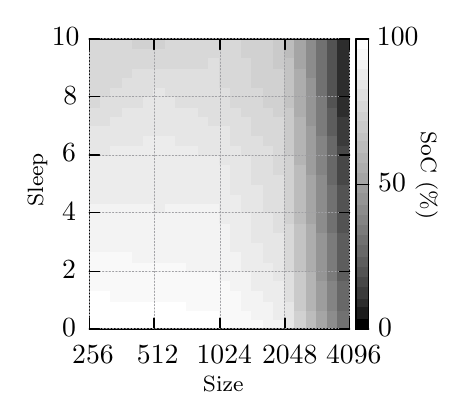
\begin{tikzpicture}[y=0.80pt, x=0.80pt, yscale=-0.600000, xscale=0.570000, inner sep=0pt, outer sep=0pt]
\begin{scope}[draw=black,line join=bevel,line cap=rect,even odd rule,line width=0.512pt]
  \begin{scope}[cm={{1.0,0.0,0.0,1.0,(0.0,0.0)}},draw=black,line join=bevel,line cap=rect,line width=0.512pt]
  \end{scope}
  \begin{scope}[cm={{1.00625,0.0,0.0,1.00625,(0.0,0.0)}},draw=black,line join=bevel,line cap=rect,line width=0.512pt]
  \end{scope}
  \begin{scope}[cm={{1.00625,0.0,0.0,1.00625,(0.0,0.0)}},draw=black,line join=bevel,line cap=rect,line width=0.512pt]
  \end{scope}
  \begin{scope}[cm={{1.00625,0.0,0.0,1.00625,(0.0,0.0)}},draw=black,line join=bevel,line cap=rect,line width=0.512pt]
  \end{scope}
  \begin{scope}[cm={{1.00625,0.0,0.0,1.00625,(0.0,0.0)}},draw=cffffff,fill=cffffff,line join=bevel,line cap=rect,line width=0.512pt]
    \path[draw,fill,even odd rule] (57.5000,268.5000) -- (57.5000,261.5000) --
      (66.5000,261.5000) -- (66.5000,268.5000) -- (57.5000,268.5000);
    \path[draw,fill,even odd rule] (66.5000,268.5000) -- (66.5000,261.5000) --
      (74.5000,261.5000) -- (74.5000,268.5000) -- (66.5000,268.5000);
    \path[draw,fill,even odd rule] (74.5000,268.5000) -- (74.5000,261.5000) --
      (83.5000,261.5000) -- (83.5000,268.5000) -- (74.5000,268.5000);
    \path[draw,fill,even odd rule] (83.5000,268.5000) -- (83.5000,261.5000) --
      (91.5000,261.5000) -- (91.5000,268.5000) -- (83.5000,268.5000);
    \path[draw,fill,even odd rule] (91.5000,268.5000) -- (91.5000,261.5000) --
      (100.5000,261.5000) -- (100.5000,268.5000) -- (91.5000,268.5000);
    \path[draw,fill,even odd rule] (100.5000,268.5000) -- (100.5000,261.5000) --
      (108.5000,261.5000) -- (108.5000,268.5000) -- (100.5000,268.5000);
    \path[draw,fill,even odd rule] (57.5000,261.5000) -- (57.5000,254.5000) --
      (66.5000,254.5000) -- (66.5000,261.5000) -- (57.5000,261.5000);
    \path[draw,fill,even odd rule] (66.5000,261.5000) -- (66.5000,254.5000) --
      (74.5000,254.5000) -- (74.5000,261.5000) -- (66.5000,261.5000);
    \path[draw,fill,even odd rule] (74.5000,261.5000) -- (74.5000,254.5000) --
      (83.5000,254.5000) -- (83.5000,261.5000) -- (74.5000,261.5000);
    \path[draw,fill,even odd rule] (83.5000,261.5000) -- (83.5000,254.5000) --
      (91.5000,254.5000) -- (91.5000,261.5000) -- (83.5000,261.5000);
    \path[draw,fill,even odd rule] (91.5000,261.5000) -- (91.5000,254.5000) --
      (100.5000,254.5000) -- (100.5000,261.5000) -- (91.5000,261.5000);
    \path[draw,fill,even odd rule] (100.5000,261.5000) -- (100.5000,254.5000) --
      (108.5000,254.5000) -- (108.5000,261.5000) -- (100.5000,261.5000);
    \path[draw,fill,even odd rule] (57.5000,254.5000) -- (57.5000,247.5000) --
      (66.5000,247.5000) -- (66.5000,254.5000) -- (57.5000,254.5000);
    \path[draw,fill,even odd rule] (66.5000,254.5000) -- (66.5000,247.5000) --
      (74.5000,247.5000) -- (74.5000,254.5000) -- (66.5000,254.5000);
    \path[draw,fill,even odd rule] (74.5000,254.5000) -- (74.5000,247.5000) --
      (83.5000,247.5000) -- (83.5000,254.5000) -- (74.5000,254.5000);
    \path[draw,fill,even odd rule] (83.5000,254.5000) -- (83.5000,247.5000) --
      (91.5000,247.5000) -- (91.5000,254.5000) -- (83.5000,254.5000);
    \path[draw,fill,even odd rule] (91.5000,254.5000) -- (91.5000,247.5000) --
      (100.5000,247.5000) -- (100.5000,254.5000) -- (91.5000,254.5000);
    \path[draw,fill,even odd rule] (100.5000,254.5000) -- (100.5000,247.5000) --
      (108.5000,247.5000) -- (108.5000,254.5000) -- (100.5000,254.5000);
    \path[draw,fill,even odd rule] (57.5000,247.5000) -- (57.5000,239.5000) --
      (66.5000,239.5000) -- (66.5000,247.5000) -- (57.5000,247.5000);
    \path[draw,fill,even odd rule] (66.5000,247.5000) -- (66.5000,239.5000) --
      (74.5000,239.5000) -- (74.5000,247.5000) -- (66.5000,247.5000);
  \end{scope}
  \begin{scope}[cm={{1.00625,0.0,0.0,1.00625,(0.0,0.0)}},draw=cf9f9f9,fill=cf9f9f9,line join=bevel,line cap=rect,line width=0.512pt]
    \path[draw,fill,even odd rule] (74.5000,247.5000) -- (74.5000,239.5000) --
      (83.5000,239.5000) -- (83.5000,247.5000) -- (74.5000,247.5000);
    \path[draw,fill,even odd rule] (83.5000,247.5000) -- (83.5000,239.5000) --
      (91.5000,239.5000) -- (91.5000,247.5000) -- (83.5000,247.5000);
    \path[draw,fill,even odd rule] (91.5000,247.5000) -- (91.5000,239.5000) --
      (100.5000,239.5000) -- (100.5000,247.5000) -- (91.5000,247.5000);
    \path[draw,fill,even odd rule] (100.5000,247.5000) -- (100.5000,239.5000) --
      (108.5000,239.5000) -- (108.5000,247.5000) -- (100.5000,247.5000);
    \path[draw,fill,even odd rule] (57.5000,239.5000) -- (57.5000,232.5000) --
      (66.5000,232.5000) -- (66.5000,239.5000) -- (57.5000,239.5000);
    \path[draw,fill,even odd rule] (66.5000,239.5000) -- (66.5000,232.5000) --
      (74.5000,232.5000) -- (74.5000,239.5000) -- (66.5000,239.5000);
    \path[draw,fill,even odd rule] (74.5000,239.5000) -- (74.5000,232.5000) --
      (83.5000,232.5000) -- (83.5000,239.5000) -- (74.5000,239.5000);
    \path[draw,fill,even odd rule] (83.5000,239.5000) -- (83.5000,232.5000) --
      (91.5000,232.5000) -- (91.5000,239.5000) -- (83.5000,239.5000);
    \path[draw,fill,even odd rule] (91.5000,239.5000) -- (91.5000,232.5000) --
      (100.5000,232.5000) -- (100.5000,239.5000) -- (91.5000,239.5000);
    \path[draw,fill,even odd rule] (100.5000,239.5000) -- (100.5000,232.5000) --
      (108.5000,232.5000) -- (108.5000,239.5000) -- (100.5000,239.5000);
    \path[draw,fill,even odd rule] (57.5000,232.5000) -- (57.5000,225.5000) --
      (66.5000,225.5000) -- (66.5000,232.5000) -- (57.5000,232.5000);
    \path[draw,fill,even odd rule] (66.5000,232.5000) -- (66.5000,225.5000) --
      (74.5000,225.5000) -- (74.5000,232.5000) -- (66.5000,232.5000);
    \path[draw,fill,even odd rule] (74.5000,232.5000) -- (74.5000,225.5000) --
      (83.5000,225.5000) -- (83.5000,232.5000) -- (74.5000,232.5000);
    \path[draw,fill,even odd rule] (83.5000,232.5000) -- (83.5000,225.5000) --
      (91.5000,225.5000) -- (91.5000,232.5000) -- (83.5000,232.5000);
    \path[draw,fill,even odd rule] (91.5000,232.5000) -- (91.5000,225.5000) --
      (100.5000,225.5000) -- (100.5000,232.5000) -- (91.5000,232.5000);
    \path[draw,fill,even odd rule] (100.5000,232.5000) -- (100.5000,225.5000) --
      (108.5000,225.5000) -- (108.5000,232.5000) -- (100.5000,232.5000);
    \path[draw,fill,even odd rule] (57.5000,225.5000) -- (57.5000,218.5000) --
      (66.5000,218.5000) -- (66.5000,225.5000) -- (57.5000,225.5000);
    \path[draw,fill,even odd rule] (66.5000,225.5000) -- (66.5000,218.5000) --
      (74.5000,218.5000) -- (74.5000,225.5000) -- (66.5000,225.5000);
    \path[draw,fill,even odd rule] (74.5000,225.5000) -- (74.5000,218.5000) --
      (83.5000,218.5000) -- (83.5000,225.5000) -- (74.5000,225.5000);
    \path[draw,fill,even odd rule] (83.5000,225.5000) -- (83.5000,218.5000) --
      (91.5000,218.5000) -- (91.5000,225.5000) -- (83.5000,225.5000);
    \path[draw,fill,even odd rule] (91.5000,225.5000) -- (91.5000,218.5000) --
      (100.5000,218.5000) -- (100.5000,225.5000) -- (91.5000,225.5000);
    \path[draw,fill,even odd rule] (100.5000,225.5000) -- (100.5000,218.5000) --
      (108.5000,218.5000) -- (108.5000,225.5000) -- (100.5000,225.5000);
    \path[draw,fill,even odd rule] (57.5000,218.5000) -- (57.5000,210.5000) --
      (66.5000,210.5000) -- (66.5000,218.5000) -- (57.5000,218.5000);
    \path[draw,fill,even odd rule] (66.5000,218.5000) -- (66.5000,210.5000) --
      (74.5000,210.5000) -- (74.5000,218.5000) -- (66.5000,218.5000);
    \path[draw,fill,even odd rule] (74.5000,218.5000) -- (74.5000,210.5000) --
      (83.5000,210.5000) -- (83.5000,218.5000) -- (74.5000,218.5000);
    \path[draw,fill,even odd rule] (83.5000,218.5000) -- (83.5000,210.5000) --
      (91.5000,210.5000) -- (91.5000,218.5000) -- (83.5000,218.5000);
  \end{scope}
  \begin{scope}[cm={{1.00625,0.0,0.0,1.00625,(0.0,0.0)}},draw=cf3f3f3,fill=cf3f3f3,line join=bevel,line cap=rect,line width=0.512pt]
    \path[draw,fill,even odd rule] (91.5000,218.5000) -- (91.5000,210.5000) --
      (100.5000,210.5000) -- (100.5000,218.5000) -- (91.5000,218.5000);
    \path[draw,fill,even odd rule] (100.5000,218.5000) -- (100.5000,210.5000) --
      (108.5000,210.5000) -- (108.5000,218.5000) -- (100.5000,218.5000);
    \path[draw,fill,even odd rule] (57.5000,210.5000) -- (57.5000,203.5000) --
      (66.5000,203.5000) -- (66.5000,210.5000) -- (57.5000,210.5000);
    \path[draw,fill,even odd rule] (66.5000,210.5000) -- (66.5000,203.5000) --
      (74.5000,203.5000) -- (74.5000,210.5000) -- (66.5000,210.5000);
    \path[draw,fill,even odd rule] (74.5000,210.5000) -- (74.5000,203.5000) --
      (83.5000,203.5000) -- (83.5000,210.5000) -- (74.5000,210.5000);
    \path[draw,fill,even odd rule] (83.5000,210.5000) -- (83.5000,203.5000) --
      (91.5000,203.5000) -- (91.5000,210.5000) -- (83.5000,210.5000);
    \path[draw,fill,even odd rule] (91.5000,210.5000) -- (91.5000,203.5000) --
      (100.5000,203.5000) -- (100.5000,210.5000) -- (91.5000,210.5000);
    \path[draw,fill,even odd rule] (100.5000,210.5000) -- (100.5000,203.5000) --
      (108.5000,203.5000) -- (108.5000,210.5000) -- (100.5000,210.5000);
    \path[draw,fill,even odd rule] (57.5000,203.5000) -- (57.5000,196.5000) --
      (66.5000,196.5000) -- (66.5000,203.5000) -- (57.5000,203.5000);
    \path[draw,fill,even odd rule] (66.5000,203.5000) -- (66.5000,196.5000) --
      (74.5000,196.5000) -- (74.5000,203.5000) -- (66.5000,203.5000);
    \path[draw,fill,even odd rule] (74.5000,203.5000) -- (74.5000,196.5000) --
      (83.5000,196.5000) -- (83.5000,203.5000) -- (74.5000,203.5000);
    \path[draw,fill,even odd rule] (83.5000,203.5000) -- (83.5000,196.5000) --
      (91.5000,196.5000) -- (91.5000,203.5000) -- (83.5000,203.5000);
    \path[draw,fill,even odd rule] (91.5000,203.5000) -- (91.5000,196.5000) --
      (100.5000,196.5000) -- (100.5000,203.5000) -- (91.5000,203.5000);
    \path[draw,fill,even odd rule] (100.5000,203.5000) -- (100.5000,196.5000) --
      (108.5000,196.5000) -- (108.5000,203.5000) -- (100.5000,203.5000);
    \path[draw,fill,even odd rule] (57.5000,196.5000) -- (57.5000,189.5000) --
      (66.5000,189.5000) -- (66.5000,196.5000) -- (57.5000,196.5000);
    \path[draw,fill,even odd rule] (66.5000,196.5000) -- (66.5000,189.5000) --
      (74.5000,189.5000) -- (74.5000,196.5000) -- (66.5000,196.5000);
    \path[draw,fill,even odd rule] (74.5000,196.5000) -- (74.5000,189.5000) --
      (83.5000,189.5000) -- (83.5000,196.5000) -- (74.5000,196.5000);
    \path[draw,fill,even odd rule] (83.5000,196.5000) -- (83.5000,189.5000) --
      (91.5000,189.5000) -- (91.5000,196.5000) -- (83.5000,196.5000);
    \path[draw,fill,even odd rule] (91.5000,196.5000) -- (91.5000,189.5000) --
      (100.5000,189.5000) -- (100.5000,196.5000) -- (91.5000,196.5000);
    \path[draw,fill,even odd rule] (100.5000,196.5000) -- (100.5000,189.5000) --
      (108.5000,189.5000) -- (108.5000,196.5000) -- (100.5000,196.5000);
    \path[draw,fill,even odd rule] (57.5000,189.5000) -- (57.5000,181.5000) --
      (66.5000,181.5000) -- (66.5000,189.5000) -- (57.5000,189.5000);
    \path[draw,fill,even odd rule] (66.5000,189.5000) -- (66.5000,181.5000) --
      (74.5000,181.5000) -- (74.5000,189.5000) -- (66.5000,189.5000);
    \path[draw,fill,even odd rule] (74.5000,189.5000) -- (74.5000,181.5000) --
      (83.5000,181.5000) -- (83.5000,189.5000) -- (74.5000,189.5000);
    \path[draw,fill,even odd rule] (83.5000,189.5000) -- (83.5000,181.5000) --
      (91.5000,181.5000) -- (91.5000,189.5000) -- (83.5000,189.5000);
    \path[draw,fill,even odd rule] (91.5000,189.5000) -- (91.5000,181.5000) --
      (100.5000,181.5000) -- (100.5000,189.5000) -- (91.5000,189.5000);
    \path[draw,fill,even odd rule] (100.5000,189.5000) -- (100.5000,181.5000) --
      (108.5000,181.5000) -- (108.5000,189.5000) -- (100.5000,189.5000);
    \path[draw,fill,even odd rule] (57.5000,181.5000) -- (57.5000,174.5000) --
      (66.5000,174.5000) -- (66.5000,181.5000) -- (57.5000,181.5000);
    \path[draw,fill,even odd rule] (66.5000,181.5000) -- (66.5000,174.5000) --
      (74.5000,174.5000) -- (74.5000,181.5000) -- (66.5000,181.5000);
    \path[draw,fill,even odd rule] (74.5000,181.5000) -- (74.5000,174.5000) --
      (83.5000,174.5000) -- (83.5000,181.5000) -- (74.5000,181.5000);
    \path[draw,fill,even odd rule] (83.5000,181.5000) -- (83.5000,174.5000) --
      (91.5000,174.5000) -- (91.5000,181.5000) -- (83.5000,181.5000);
    \path[draw,fill,even odd rule] (91.5000,181.5000) -- (91.5000,174.5000) --
      (100.5000,174.5000) -- (100.5000,181.5000) -- (91.5000,181.5000);
    \path[draw,fill,even odd rule] (100.5000,181.5000) -- (100.5000,174.5000) --
      (108.5000,174.5000) -- (108.5000,181.5000) -- (100.5000,181.5000);
  \end{scope}
  \begin{scope}[cm={{1.00625,0.0,0.0,1.00625,(0.0,0.0)}},draw=cececec,fill=cececec,line join=bevel,line cap=rect,line width=0.512pt]
    \path[draw,fill,even odd rule] (57.5000,174.5000) -- (57.5000,167.5000) --
      (66.5000,167.5000) -- (66.5000,174.5000) -- (57.5000,174.5000);
    \path[draw,fill,even odd rule] (66.5000,174.5000) -- (66.5000,167.5000) --
      (74.5000,167.5000) -- (74.5000,174.5000) -- (66.5000,174.5000);
    \path[draw,fill,even odd rule] (74.5000,174.5000) -- (74.5000,167.5000) --
      (83.5000,167.5000) -- (83.5000,174.5000) -- (74.5000,174.5000);
    \path[draw,fill,even odd rule] (83.5000,174.5000) -- (83.5000,167.5000) --
      (91.5000,167.5000) -- (91.5000,174.5000) -- (83.5000,174.5000);
    \path[draw,fill,even odd rule] (91.5000,174.5000) -- (91.5000,167.5000) --
      (100.5000,167.5000) -- (100.5000,174.5000) -- (91.5000,174.5000);
    \path[draw,fill,even odd rule] (100.5000,174.5000) -- (100.5000,167.5000) --
      (108.5000,167.5000) -- (108.5000,174.5000) -- (100.5000,174.5000);
    \path[draw,fill,even odd rule] (57.5000,167.5000) -- (57.5000,160.5000) --
      (66.5000,160.5000) -- (66.5000,167.5000) -- (57.5000,167.5000);
    \path[draw,fill,even odd rule] (66.5000,167.5000) -- (66.5000,160.5000) --
      (74.5000,160.5000) -- (74.5000,167.5000) -- (66.5000,167.5000);
    \path[draw,fill,even odd rule] (74.5000,167.5000) -- (74.5000,160.5000) --
      (83.5000,160.5000) -- (83.5000,167.5000) -- (74.5000,167.5000);
    \path[draw,fill,even odd rule] (83.5000,167.5000) -- (83.5000,160.5000) --
      (91.5000,160.5000) -- (91.5000,167.5000) -- (83.5000,167.5000);
    \path[draw,fill,even odd rule] (91.5000,167.5000) -- (91.5000,160.5000) --
      (100.5000,160.5000) -- (100.5000,167.5000) -- (91.5000,167.5000);
    \path[draw,fill,even odd rule] (100.5000,167.5000) -- (100.5000,160.5000) --
      (108.5000,160.5000) -- (108.5000,167.5000) -- (100.5000,167.5000);
    \path[draw,fill,even odd rule] (57.5000,160.5000) -- (57.5000,152.5000) --
      (66.5000,152.5000) -- (66.5000,160.5000) -- (57.5000,160.5000);
    \path[draw,fill,even odd rule] (66.5000,160.5000) -- (66.5000,152.5000) --
      (74.5000,152.5000) -- (74.5000,160.5000) -- (66.5000,160.5000);
    \path[draw,fill,even odd rule] (74.5000,160.5000) -- (74.5000,152.5000) --
      (83.5000,152.5000) -- (83.5000,160.5000) -- (74.5000,160.5000);
    \path[draw,fill,even odd rule] (83.5000,160.5000) -- (83.5000,152.5000) --
      (91.5000,152.5000) -- (91.5000,160.5000) -- (83.5000,160.5000);
    \path[draw,fill,even odd rule] (91.5000,160.5000) -- (91.5000,152.5000) --
      (100.5000,152.5000) -- (100.5000,160.5000) -- (91.5000,160.5000);
    \path[draw,fill,even odd rule] (100.5000,160.5000) -- (100.5000,152.5000) --
      (108.5000,152.5000) -- (108.5000,160.5000) -- (100.5000,160.5000);
    \path[draw,fill,even odd rule] (57.5000,152.5000) -- (57.5000,145.5000) --
      (66.5000,145.5000) -- (66.5000,152.5000) -- (57.5000,152.5000);
    \path[draw,fill,even odd rule] (66.5000,152.5000) -- (66.5000,145.5000) --
      (74.5000,145.5000) -- (74.5000,152.5000) -- (66.5000,152.5000);
    \path[draw,fill,even odd rule] (74.5000,152.5000) -- (74.5000,145.5000) --
      (83.5000,145.5000) -- (83.5000,152.5000) -- (74.5000,152.5000);
    \path[draw,fill,even odd rule] (83.5000,152.5000) -- (83.5000,145.5000) --
      (91.5000,145.5000) -- (91.5000,152.5000) -- (83.5000,152.5000);
    \path[draw,fill,even odd rule] (91.5000,152.5000) -- (91.5000,145.5000) --
      (100.5000,145.5000) -- (100.5000,152.5000) -- (91.5000,152.5000);
    \path[draw,fill,even odd rule] (100.5000,152.5000) -- (100.5000,145.5000) --
      (108.5000,145.5000) -- (108.5000,152.5000) -- (100.5000,152.5000);
    \path[draw,fill,even odd rule] (57.5000,145.5000) -- (57.5000,138.5000) --
      (66.5000,138.5000) -- (66.5000,145.5000) -- (57.5000,145.5000);
    \path[draw,fill,even odd rule] (66.5000,145.5000) -- (66.5000,138.5000) --
      (74.5000,138.5000) -- (74.5000,145.5000) -- (66.5000,145.5000);
    \path[draw,fill,even odd rule] (74.5000,145.5000) -- (74.5000,138.5000) --
      (83.5000,138.5000) -- (83.5000,145.5000) -- (74.5000,145.5000);
    \path[draw,fill,even odd rule] (83.5000,145.5000) -- (83.5000,138.5000) --
      (91.5000,138.5000) -- (91.5000,145.5000) -- (83.5000,145.5000);
    \path[draw,fill,even odd rule] (91.5000,145.5000) -- (91.5000,138.5000) --
      (100.5000,138.5000) -- (100.5000,145.5000) -- (91.5000,145.5000);
    \path[draw,fill,even odd rule] (100.5000,145.5000) -- (100.5000,138.5000) --
      (108.5000,138.5000) -- (108.5000,145.5000) -- (100.5000,145.5000);
  \end{scope}
  \begin{scope}[cm={{1.00625,0.0,0.0,1.00625,(0.0,0.0)}},draw=ce6e6e6,fill=ce6e6e6,line join=bevel,line cap=rect,line width=0.512pt]
    \path[draw,fill,even odd rule] (57.5000,138.5000) -- (57.5000,131.5000) --
      (66.5000,131.5000) -- (66.5000,138.5000) -- (57.5000,138.5000);
    \path[draw,fill,even odd rule] (66.5000,138.5000) -- (66.5000,131.5000) --
      (74.5000,131.5000) -- (74.5000,138.5000) -- (66.5000,138.5000);
  \end{scope}
  \begin{scope}[cm={{1.00625,0.0,0.0,1.00625,(0.0,0.0)}},draw=cececec,fill=cececec,line join=bevel,line cap=rect,line width=0.512pt]
    \path[draw,fill,even odd rule] (74.5000,138.5000) -- (74.5000,131.5000) --
      (83.5000,131.5000) -- (83.5000,138.5000) -- (74.5000,138.5000);
    \path[draw,fill,even odd rule] (83.5000,138.5000) -- (83.5000,131.5000) --
      (91.5000,131.5000) -- (91.5000,138.5000) -- (83.5000,138.5000);
    \path[draw,fill,even odd rule] (91.5000,138.5000) -- (91.5000,131.5000) --
      (100.5000,131.5000) -- (100.5000,138.5000) -- (91.5000,138.5000);
    \path[draw,fill,even odd rule] (100.5000,138.5000) -- (100.5000,131.5000) --
      (108.5000,131.5000) -- (108.5000,138.5000) -- (100.5000,138.5000);
  \end{scope}
  \begin{scope}[cm={{1.00625,0.0,0.0,1.00625,(0.0,0.0)}},draw=ce6e6e6,fill=ce6e6e6,line join=bevel,line cap=rect,line width=0.512pt]
    \path[draw,fill,even odd rule] (57.5000,131.5000) -- (57.5000,123.5000) --
      (66.5000,123.5000) -- (66.5000,131.5000) -- (57.5000,131.5000);
    \path[draw,fill,even odd rule] (66.5000,131.5000) -- (66.5000,123.5000) --
      (74.5000,123.5000) -- (74.5000,131.5000) -- (66.5000,131.5000);
    \path[draw,fill,even odd rule] (74.5000,131.5000) -- (74.5000,123.5000) --
      (83.5000,123.5000) -- (83.5000,131.5000) -- (74.5000,131.5000);
    \path[draw,fill,even odd rule] (83.5000,131.5000) -- (83.5000,123.5000) --
      (91.5000,123.5000) -- (91.5000,131.5000) -- (83.5000,131.5000);
    \path[draw,fill,even odd rule] (91.5000,131.5000) -- (91.5000,123.5000) --
      (100.5000,123.5000) -- (100.5000,131.5000) -- (91.5000,131.5000);
  \end{scope}
  \begin{scope}[cm={{1.00625,0.0,0.0,1.00625,(0.0,0.0)}},draw=cececec,fill=cececec,line join=bevel,line cap=rect,line width=0.512pt]
    \path[draw,fill,even odd rule] (100.5000,131.5000) -- (100.5000,123.5000) --
      (108.5000,123.5000) -- (108.5000,131.5000) -- (100.5000,131.5000);
  \end{scope}
  \begin{scope}[cm={{1.00625,0.0,0.0,1.00625,(0.0,0.0)}},draw=ce6e6e6,fill=ce6e6e6,line join=bevel,line cap=rect,line width=0.512pt]
    \path[draw,fill,even odd rule] (57.5000,123.5000) -- (57.5000,116.5000) --
      (66.5000,116.5000) -- (66.5000,123.5000) -- (57.5000,123.5000);
    \path[draw,fill,even odd rule] (66.5000,123.5000) -- (66.5000,116.5000) --
      (74.5000,116.5000) -- (74.5000,123.5000) -- (66.5000,123.5000);
    \path[draw,fill,even odd rule] (74.5000,123.5000) -- (74.5000,116.5000) --
      (83.5000,116.5000) -- (83.5000,123.5000) -- (74.5000,123.5000);
    \path[draw,fill,even odd rule] (83.5000,123.5000) -- (83.5000,116.5000) --
      (91.5000,116.5000) -- (91.5000,123.5000) -- (83.5000,123.5000);
    \path[draw,fill,even odd rule] (91.5000,123.5000) -- (91.5000,116.5000) --
      (100.5000,116.5000) -- (100.5000,123.5000) -- (91.5000,123.5000);
    \path[draw,fill,even odd rule] (100.5000,123.5000) -- (100.5000,116.5000) --
      (108.5000,116.5000) -- (108.5000,123.5000) -- (100.5000,123.5000);
  \end{scope}
  \begin{scope}[cm={{1.00625,0.0,0.0,1.00625,(0.0,0.0)}},draw=cdfdfdf,fill=cdfdfdf,line join=bevel,line cap=rect,line width=0.512pt]
    \path[draw,fill,even odd rule] (57.5000,116.5000) -- (57.5000,109.5000) --
      (66.5000,109.5000) -- (66.5000,116.5000) -- (57.5000,116.5000);
    \path[draw,fill,even odd rule] (66.5000,116.5000) -- (66.5000,109.5000) --
      (74.5000,109.5000) -- (74.5000,116.5000) -- (66.5000,116.5000);
  \end{scope}
  \begin{scope}[cm={{1.00625,0.0,0.0,1.00625,(0.0,0.0)}},draw=ce6e6e6,fill=ce6e6e6,line join=bevel,line cap=rect,line width=0.512pt]
    \path[draw,fill,even odd rule] (74.5000,116.5000) -- (74.5000,109.5000) --
      (83.5000,109.5000) -- (83.5000,116.5000) -- (74.5000,116.5000);
    \path[draw,fill,even odd rule] (83.5000,116.5000) -- (83.5000,109.5000) --
      (91.5000,109.5000) -- (91.5000,116.5000) -- (83.5000,116.5000);
    \path[draw,fill,even odd rule] (91.5000,116.5000) -- (91.5000,109.5000) --
      (100.5000,109.5000) -- (100.5000,116.5000) -- (91.5000,116.5000);
    \path[draw,fill,even odd rule] (100.5000,116.5000) -- (100.5000,109.5000) --
      (108.5000,109.5000) -- (108.5000,116.5000) -- (100.5000,116.5000);
  \end{scope}
  \begin{scope}[cm={{1.00625,0.0,0.0,1.00625,(0.0,0.0)}},draw=cdfdfdf,fill=cdfdfdf,line join=bevel,line cap=rect,line width=0.512pt]
    \path[draw,fill,even odd rule] (57.5000,109.5000) -- (57.5000,102.5000) --
      (66.5000,102.5000) -- (66.5000,109.5000) -- (57.5000,109.5000);
    \path[draw,fill,even odd rule] (66.5000,109.5000) -- (66.5000,102.5000) --
      (74.5000,102.5000) -- (74.5000,109.5000) -- (66.5000,109.5000);
    \path[draw,fill,even odd rule] (74.5000,109.5000) -- (74.5000,102.5000) --
      (83.5000,102.5000) -- (83.5000,109.5000) -- (74.5000,109.5000);
  \end{scope}
  \begin{scope}[cm={{1.00625,0.0,0.0,1.00625,(0.0,0.0)}},draw=ce6e6e6,fill=ce6e6e6,line join=bevel,line cap=rect,line width=0.512pt]
    \path[draw,fill,even odd rule] (83.5000,109.5000) -- (83.5000,102.5000) --
      (91.5000,102.5000) -- (91.5000,109.5000) -- (83.5000,109.5000);
    \path[draw,fill,even odd rule] (91.5000,109.5000) -- (91.5000,102.5000) --
      (100.5000,102.5000) -- (100.5000,109.5000) -- (91.5000,109.5000);
    \path[draw,fill,even odd rule] (100.5000,109.5000) -- (100.5000,102.5000) --
      (108.5000,102.5000) -- (108.5000,109.5000) -- (100.5000,109.5000);
  \end{scope}
  \begin{scope}[cm={{1.00625,0.0,0.0,1.00625,(0.0,0.0)}},draw=cd8d8d8,fill=cd8d8d8,line join=bevel,line cap=rect,line width=0.512pt]
    \path[draw,fill,even odd rule] (57.5000,102.5000) -- (57.5000,94.5000) --
      (66.5000,94.5000) -- (66.5000,102.5000) -- (57.5000,102.5000);
  \end{scope}
  \begin{scope}[cm={{1.00625,0.0,0.0,1.00625,(0.0,0.0)}},draw=cdfdfdf,fill=cdfdfdf,line join=bevel,line cap=rect,line width=0.512pt]
    \path[draw,fill,even odd rule] (66.5000,102.5000) -- (66.5000,94.5000) --
      (74.5000,94.5000) -- (74.5000,102.5000) -- (66.5000,102.5000);
    \path[draw,fill,even odd rule] (74.5000,102.5000) -- (74.5000,94.5000) --
      (83.5000,94.5000) -- (83.5000,102.5000) -- (74.5000,102.5000);
    \path[draw,fill,even odd rule] (83.5000,102.5000) -- (83.5000,94.5000) --
      (91.5000,94.5000) -- (91.5000,102.5000) -- (83.5000,102.5000);
    \path[draw,fill,even odd rule] (91.5000,102.5000) -- (91.5000,94.5000) --
      (100.5000,94.5000) -- (100.5000,102.5000) -- (91.5000,102.5000);
  \end{scope}
  \begin{scope}[cm={{1.00625,0.0,0.0,1.00625,(0.0,0.0)}},draw=ce6e6e6,fill=ce6e6e6,line join=bevel,line cap=rect,line width=0.512pt]
    \path[draw,fill,even odd rule] (100.5000,102.5000) -- (100.5000,94.5000) --
      (108.5000,94.5000) -- (108.5000,102.5000) -- (100.5000,102.5000);
  \end{scope}
  \begin{scope}[cm={{1.00625,0.0,0.0,1.00625,(0.0,0.0)}},draw=cd8d8d8,fill=cd8d8d8,line join=bevel,line cap=rect,line width=0.512pt]
    \path[draw,fill,even odd rule] (57.5000,94.5000) -- (57.5000,87.5000) --
      (66.5000,87.5000) -- (66.5000,94.5000) -- (57.5000,94.5000);
    \path[draw,fill,even odd rule] (66.5000,94.5000) -- (66.5000,87.5000) --
      (74.5000,87.5000) -- (74.5000,94.5000) -- (66.5000,94.5000);
  \end{scope}
  \begin{scope}[cm={{1.00625,0.0,0.0,1.00625,(0.0,0.0)}},draw=cdfdfdf,fill=cdfdfdf,line join=bevel,line cap=rect,line width=0.512pt]
    \path[draw,fill,even odd rule] (74.5000,94.5000) -- (74.5000,87.5000) --
      (83.5000,87.5000) -- (83.5000,94.5000) -- (74.5000,94.5000);
    \path[draw,fill,even odd rule] (83.5000,94.5000) -- (83.5000,87.5000) --
      (91.5000,87.5000) -- (91.5000,94.5000) -- (83.5000,94.5000);
    \path[draw,fill,even odd rule] (91.5000,94.5000) -- (91.5000,87.5000) --
      (100.5000,87.5000) -- (100.5000,94.5000) -- (91.5000,94.5000);
    \path[draw,fill,even odd rule] (100.5000,94.5000) -- (100.5000,87.5000) --
      (108.5000,87.5000) -- (108.5000,94.5000) -- (100.5000,94.5000);
  \end{scope}
  \begin{scope}[cm={{1.00625,0.0,0.0,1.00625,(0.0,0.0)}},draw=cd8d8d8,fill=cd8d8d8,line join=bevel,line cap=rect,line width=0.512pt]
    \path[draw,fill,even odd rule] (57.5000,87.5000) -- (57.5000,80.5000) --
      (66.5000,80.5000) -- (66.5000,87.5000) -- (57.5000,87.5000);
    \path[draw,fill,even odd rule] (66.5000,87.5000) -- (66.5000,80.5000) --
      (74.5000,80.5000) -- (74.5000,87.5000) -- (66.5000,87.5000);
    \path[draw,fill,even odd rule] (74.5000,87.5000) -- (74.5000,80.5000) --
      (83.5000,80.5000) -- (83.5000,87.5000) -- (74.5000,87.5000);
  \end{scope}
  \begin{scope}[cm={{1.00625,0.0,0.0,1.00625,(0.0,0.0)}},draw=cdfdfdf,fill=cdfdfdf,line join=bevel,line cap=rect,line width=0.512pt]
    \path[draw,fill,even odd rule] (83.5000,87.5000) -- (83.5000,80.5000) --
      (91.5000,80.5000) -- (91.5000,87.5000) -- (83.5000,87.5000);
    \path[draw,fill,even odd rule] (91.5000,87.5000) -- (91.5000,80.5000) --
      (100.5000,80.5000) -- (100.5000,87.5000) -- (91.5000,87.5000);
    \path[draw,fill,even odd rule] (100.5000,87.5000) -- (100.5000,80.5000) --
      (108.5000,80.5000) -- (108.5000,87.5000) -- (100.5000,87.5000);
  \end{scope}
  \begin{scope}[cm={{1.00625,0.0,0.0,1.00625,(0.0,0.0)}},draw=cd8d8d8,fill=cd8d8d8,line join=bevel,line cap=rect,line width=0.512pt]
    \path[draw,fill,even odd rule] (57.5000,80.5000) -- (57.5000,73.5000) --
      (66.5000,73.5000) -- (66.5000,80.5000) -- (57.5000,80.5000);
    \path[draw,fill,even odd rule] (66.5000,80.5000) -- (66.5000,73.5000) --
      (74.5000,73.5000) -- (74.5000,80.5000) -- (66.5000,80.5000);
    \path[draw,fill,even odd rule] (74.5000,80.5000) -- (74.5000,73.5000) --
      (83.5000,73.5000) -- (83.5000,80.5000) -- (74.5000,80.5000);
    \path[draw,fill,even odd rule] (83.5000,80.5000) -- (83.5000,73.5000) --
      (91.5000,73.5000) -- (91.5000,80.5000) -- (83.5000,80.5000);
  \end{scope}
  \begin{scope}[cm={{1.00625,0.0,0.0,1.00625,(0.0,0.0)}},draw=cdfdfdf,fill=cdfdfdf,line join=bevel,line cap=rect,line width=0.512pt]
    \path[draw,fill,even odd rule] (91.5000,80.5000) -- (91.5000,73.5000) --
      (100.5000,73.5000) -- (100.5000,80.5000) -- (91.5000,80.5000);
    \path[draw,fill,even odd rule] (100.5000,80.5000) -- (100.5000,73.5000) --
      (108.5000,73.5000) -- (108.5000,80.5000) -- (100.5000,80.5000);
  \end{scope}
  \begin{scope}[cm={{1.00625,0.0,0.0,1.00625,(0.0,0.0)}},draw=cd8d8d8,fill=cd8d8d8,line join=bevel,line cap=rect,line width=0.512pt]
    \path[draw,fill,even odd rule] (57.5000,73.5000) -- (57.5000,65.5000) --
      (66.5000,65.5000) -- (66.5000,73.5000) -- (57.5000,73.5000);
    \path[draw,fill,even odd rule] (66.5000,73.5000) -- (66.5000,65.5000) --
      (74.5000,65.5000) -- (74.5000,73.5000) -- (66.5000,73.5000);
    \path[draw,fill,even odd rule] (74.5000,73.5000) -- (74.5000,65.5000) --
      (83.5000,65.5000) -- (83.5000,73.5000) -- (74.5000,73.5000);
    \path[draw,fill,even odd rule] (83.5000,73.5000) -- (83.5000,65.5000) --
      (91.5000,65.5000) -- (91.5000,73.5000) -- (83.5000,73.5000);
    \path[draw,fill,even odd rule] (91.5000,73.5000) -- (91.5000,65.5000) --
      (100.5000,65.5000) -- (100.5000,73.5000) -- (91.5000,73.5000);
    \path[draw,fill,even odd rule] (100.5000,73.5000) -- (100.5000,65.5000) --
      (108.5000,65.5000) -- (108.5000,73.5000) -- (100.5000,73.5000);
    \path[draw,fill,even odd rule] (57.5000,65.5000) -- (57.5000,58.5000) --
      (66.5000,58.5000) -- (66.5000,65.5000) -- (57.5000,65.5000);
    \path[draw,fill,even odd rule] (66.5000,65.5000) -- (66.5000,58.5000) --
      (74.5000,58.5000) -- (74.5000,65.5000) -- (66.5000,65.5000);
    \path[draw,fill,even odd rule] (74.5000,65.5000) -- (74.5000,58.5000) --
      (83.5000,58.5000) -- (83.5000,65.5000) -- (74.5000,65.5000);
    \path[draw,fill,even odd rule] (83.5000,65.5000) -- (83.5000,58.5000) --
      (91.5000,58.5000) -- (91.5000,65.5000) -- (83.5000,65.5000);
    \path[draw,fill,even odd rule] (91.5000,65.5000) -- (91.5000,58.5000) --
      (100.5000,58.5000) -- (100.5000,65.5000) -- (91.5000,65.5000);
    \path[draw,fill,even odd rule] (100.5000,65.5000) -- (100.5000,58.5000) --
      (108.5000,58.5000) -- (108.5000,65.5000) -- (100.5000,65.5000);
    \path[draw,fill,even odd rule] (57.5000,58.5000) -- (57.5000,51.5000) --
      (66.5000,51.5000) -- (66.5000,58.5000) -- (57.5000,58.5000);
    \path[draw,fill,even odd rule] (66.5000,58.5000) -- (66.5000,51.5000) --
      (74.5000,51.5000) -- (74.5000,58.5000) -- (66.5000,58.5000);
    \path[draw,fill,even odd rule] (74.5000,58.5000) -- (74.5000,51.5000) --
      (83.5000,51.5000) -- (83.5000,58.5000) -- (74.5000,58.5000);
    \path[draw,fill,even odd rule] (83.5000,58.5000) -- (83.5000,51.5000) --
      (91.5000,51.5000) -- (91.5000,58.5000) -- (83.5000,58.5000);
  \end{scope}
  \begin{scope}[cm={{1.00625,0.0,0.0,1.00625,(0.0,0.0)}},draw=cd1d1d1,fill=cd1d1d1,line join=bevel,line cap=rect,line width=0.512pt]
    \path[draw,fill,even odd rule] (91.5000,58.5000) -- (91.5000,51.5000) --
      (100.5000,51.5000) -- (100.5000,58.5000) -- (91.5000,58.5000);
    \path[draw,fill,even odd rule] (100.5000,58.5000) -- (100.5000,51.5000) --
      (108.5000,51.5000) -- (108.5000,58.5000) -- (100.5000,58.5000);
  \end{scope}
  \begin{scope}[cm={{1.00625,0.0,0.0,1.00625,(0.0,0.0)}},draw=cffffff,fill=cffffff,line join=bevel,line cap=rect,line width=0.512pt]
    \path[draw,fill,even odd rule] (108.5000,268.5000) -- (108.5000,261.5000) --
      (117.5000,261.5000) -- (117.5000,268.5000) -- (108.5000,268.5000);
    \path[draw,fill,even odd rule] (117.5000,268.5000) -- (117.5000,261.5000) --
      (125.5000,261.5000) -- (125.5000,268.5000) -- (117.5000,268.5000);
    \path[draw,fill,even odd rule] (125.5000,268.5000) -- (125.5000,261.5000) --
      (134.5000,261.5000) -- (134.5000,268.5000) -- (125.5000,268.5000);
    \path[draw,fill,even odd rule] (134.5000,268.5000) -- (134.5000,261.5000) --
      (143.5000,261.5000) -- (143.5000,268.5000) -- (134.5000,268.5000);
    \path[draw,fill,even odd rule] (143.5000,268.5000) -- (143.5000,261.5000) --
      (151.5000,261.5000) -- (151.5000,268.5000) -- (143.5000,268.5000);
    \path[draw,fill,even odd rule] (151.5000,268.5000) -- (151.5000,261.5000) --
      (160.5000,261.5000) -- (160.5000,268.5000) -- (151.5000,268.5000);
    \path[draw,fill,even odd rule] (108.5000,261.5000) -- (108.5000,254.5000) --
      (117.5000,254.5000) -- (117.5000,261.5000) -- (108.5000,261.5000);
    \path[draw,fill,even odd rule] (117.5000,261.5000) -- (117.5000,254.5000) --
      (125.5000,254.5000) -- (125.5000,261.5000) -- (117.5000,261.5000);
    \path[draw,fill,even odd rule] (125.5000,261.5000) -- (125.5000,254.5000) --
      (134.5000,254.5000) -- (134.5000,261.5000) -- (125.5000,261.5000);
    \path[draw,fill,even odd rule] (134.5000,261.5000) -- (134.5000,254.5000) --
      (143.5000,254.5000) -- (143.5000,261.5000) -- (134.5000,261.5000);
    \path[draw,fill,even odd rule] (143.5000,261.5000) -- (143.5000,254.5000) --
      (151.5000,254.5000) -- (151.5000,261.5000) -- (143.5000,261.5000);
    \path[draw,fill,even odd rule] (151.5000,261.5000) -- (151.5000,254.5000) --
      (160.5000,254.5000) -- (160.5000,261.5000) -- (151.5000,261.5000);
    \path[draw,fill,even odd rule] (108.5000,254.5000) -- (108.5000,247.5000) --
      (117.5000,247.5000) -- (117.5000,254.5000) -- (108.5000,254.5000);
    \path[draw,fill,even odd rule] (117.5000,254.5000) -- (117.5000,247.5000) --
      (125.5000,247.5000) -- (125.5000,254.5000) -- (117.5000,254.5000);
    \path[draw,fill,even odd rule] (125.5000,254.5000) -- (125.5000,247.5000) --
      (134.5000,247.5000) -- (134.5000,254.5000) -- (125.5000,254.5000);
  \end{scope}
  \begin{scope}[cm={{1.00625,0.0,0.0,1.00625,(0.0,0.0)}},draw=cf9f9f9,fill=cf9f9f9,line join=bevel,line cap=rect,line width=0.512pt]
    \path[draw,fill,even odd rule] (134.5000,254.5000) -- (134.5000,247.5000) --
      (143.5000,247.5000) -- (143.5000,254.5000) -- (134.5000,254.5000);
    \path[draw,fill,even odd rule] (143.5000,254.5000) -- (143.5000,247.5000) --
      (151.5000,247.5000) -- (151.5000,254.5000) -- (143.5000,254.5000);
    \path[draw,fill,even odd rule] (151.5000,254.5000) -- (151.5000,247.5000) --
      (160.5000,247.5000) -- (160.5000,254.5000) -- (151.5000,254.5000);
    \path[draw,fill,even odd rule] (108.5000,247.5000) -- (108.5000,239.5000) --
      (117.5000,239.5000) -- (117.5000,247.5000) -- (108.5000,247.5000);
    \path[draw,fill,even odd rule] (117.5000,247.5000) -- (117.5000,239.5000) --
      (125.5000,239.5000) -- (125.5000,247.5000) -- (117.5000,247.5000);
    \path[draw,fill,even odd rule] (125.5000,247.5000) -- (125.5000,239.5000) --
      (134.5000,239.5000) -- (134.5000,247.5000) -- (125.5000,247.5000);
    \path[draw,fill,even odd rule] (134.5000,247.5000) -- (134.5000,239.5000) --
      (143.5000,239.5000) -- (143.5000,247.5000) -- (134.5000,247.5000);
    \path[draw,fill,even odd rule] (143.5000,247.5000) -- (143.5000,239.5000) --
      (151.5000,239.5000) -- (151.5000,247.5000) -- (143.5000,247.5000);
    \path[draw,fill,even odd rule] (151.5000,247.5000) -- (151.5000,239.5000) --
      (160.5000,239.5000) -- (160.5000,247.5000) -- (151.5000,247.5000);
    \path[draw,fill,even odd rule] (108.5000,239.5000) -- (108.5000,232.5000) --
      (117.5000,232.5000) -- (117.5000,239.5000) -- (108.5000,239.5000);
    \path[draw,fill,even odd rule] (117.5000,239.5000) -- (117.5000,232.5000) --
      (125.5000,232.5000) -- (125.5000,239.5000) -- (117.5000,239.5000);
    \path[draw,fill,even odd rule] (125.5000,239.5000) -- (125.5000,232.5000) --
      (134.5000,232.5000) -- (134.5000,239.5000) -- (125.5000,239.5000);
    \path[draw,fill,even odd rule] (134.5000,239.5000) -- (134.5000,232.5000) --
      (143.5000,232.5000) -- (143.5000,239.5000) -- (134.5000,239.5000);
    \path[draw,fill,even odd rule] (143.5000,239.5000) -- (143.5000,232.5000) --
      (151.5000,232.5000) -- (151.5000,239.5000) -- (143.5000,239.5000);
    \path[draw,fill,even odd rule] (151.5000,239.5000) -- (151.5000,232.5000) --
      (160.5000,232.5000) -- (160.5000,239.5000) -- (151.5000,239.5000);
    \path[draw,fill,even odd rule] (108.5000,232.5000) -- (108.5000,225.5000) --
      (117.5000,225.5000) -- (117.5000,232.5000) -- (108.5000,232.5000);
    \path[draw,fill,even odd rule] (117.5000,232.5000) -- (117.5000,225.5000) --
      (125.5000,225.5000) -- (125.5000,232.5000) -- (117.5000,232.5000);
    \path[draw,fill,even odd rule] (125.5000,232.5000) -- (125.5000,225.5000) --
      (134.5000,225.5000) -- (134.5000,232.5000) -- (125.5000,232.5000);
    \path[draw,fill,even odd rule] (134.5000,232.5000) -- (134.5000,225.5000) --
      (143.5000,225.5000) -- (143.5000,232.5000) -- (134.5000,232.5000);
    \path[draw,fill,even odd rule] (143.5000,232.5000) -- (143.5000,225.5000) --
      (151.5000,225.5000) -- (151.5000,232.5000) -- (143.5000,232.5000);
    \path[draw,fill,even odd rule] (151.5000,232.5000) -- (151.5000,225.5000) --
      (160.5000,225.5000) -- (160.5000,232.5000) -- (151.5000,232.5000);
    \path[draw,fill,even odd rule] (108.5000,225.5000) -- (108.5000,218.5000) --
      (117.5000,218.5000) -- (117.5000,225.5000) -- (108.5000,225.5000);
    \path[draw,fill,even odd rule] (117.5000,225.5000) -- (117.5000,218.5000) --
      (125.5000,218.5000) -- (125.5000,225.5000) -- (117.5000,225.5000);
    \path[draw,fill,even odd rule] (125.5000,225.5000) -- (125.5000,218.5000) --
      (134.5000,218.5000) -- (134.5000,225.5000) -- (125.5000,225.5000);
  \end{scope}
  \begin{scope}[cm={{1.00625,0.0,0.0,1.00625,(0.0,0.0)}},draw=cf3f3f3,fill=cf3f3f3,line join=bevel,line cap=rect,line width=0.512pt]
    \path[draw,fill,even odd rule] (134.5000,225.5000) -- (134.5000,218.5000) --
      (143.5000,218.5000) -- (143.5000,225.5000) -- (134.5000,225.5000);
    \path[draw,fill,even odd rule] (143.5000,225.5000) -- (143.5000,218.5000) --
      (151.5000,218.5000) -- (151.5000,225.5000) -- (143.5000,225.5000);
    \path[draw,fill,even odd rule] (151.5000,225.5000) -- (151.5000,218.5000) --
      (160.5000,218.5000) -- (160.5000,225.5000) -- (151.5000,225.5000);
    \path[draw,fill,even odd rule] (108.5000,218.5000) -- (108.5000,210.5000) --
      (117.5000,210.5000) -- (117.5000,218.5000) -- (108.5000,218.5000);
    \path[draw,fill,even odd rule] (117.5000,218.5000) -- (117.5000,210.5000) --
      (125.5000,210.5000) -- (125.5000,218.5000) -- (117.5000,218.5000);
    \path[draw,fill,even odd rule] (125.5000,218.5000) -- (125.5000,210.5000) --
      (134.5000,210.5000) -- (134.5000,218.5000) -- (125.5000,218.5000);
    \path[draw,fill,even odd rule] (134.5000,218.5000) -- (134.5000,210.5000) --
      (143.5000,210.5000) -- (143.5000,218.5000) -- (134.5000,218.5000);
    \path[draw,fill,even odd rule] (143.5000,218.5000) -- (143.5000,210.5000) --
      (151.5000,210.5000) -- (151.5000,218.5000) -- (143.5000,218.5000);
    \path[draw,fill,even odd rule] (151.5000,218.5000) -- (151.5000,210.5000) --
      (160.5000,210.5000) -- (160.5000,218.5000) -- (151.5000,218.5000);
    \path[draw,fill,even odd rule] (108.5000,210.5000) -- (108.5000,203.5000) --
      (117.5000,203.5000) -- (117.5000,210.5000) -- (108.5000,210.5000);
    \path[draw,fill,even odd rule] (117.5000,210.5000) -- (117.5000,203.5000) --
      (125.5000,203.5000) -- (125.5000,210.5000) -- (117.5000,210.5000);
    \path[draw,fill,even odd rule] (125.5000,210.5000) -- (125.5000,203.5000) --
      (134.5000,203.5000) -- (134.5000,210.5000) -- (125.5000,210.5000);
    \path[draw,fill,even odd rule] (134.5000,210.5000) -- (134.5000,203.5000) --
      (143.5000,203.5000) -- (143.5000,210.5000) -- (134.5000,210.5000);
    \path[draw,fill,even odd rule] (143.5000,210.5000) -- (143.5000,203.5000) --
      (151.5000,203.5000) -- (151.5000,210.5000) -- (143.5000,210.5000);
    \path[draw,fill,even odd rule] (151.5000,210.5000) -- (151.5000,203.5000) --
      (160.5000,203.5000) -- (160.5000,210.5000) -- (151.5000,210.5000);
    \path[draw,fill,even odd rule] (108.5000,203.5000) -- (108.5000,196.5000) --
      (117.5000,196.5000) -- (117.5000,203.5000) -- (108.5000,203.5000);
    \path[draw,fill,even odd rule] (117.5000,203.5000) -- (117.5000,196.5000) --
      (125.5000,196.5000) -- (125.5000,203.5000) -- (117.5000,203.5000);
    \path[draw,fill,even odd rule] (125.5000,203.5000) -- (125.5000,196.5000) --
      (134.5000,196.5000) -- (134.5000,203.5000) -- (125.5000,203.5000);
    \path[draw,fill,even odd rule] (134.5000,203.5000) -- (134.5000,196.5000) --
      (143.5000,196.5000) -- (143.5000,203.5000) -- (134.5000,203.5000);
    \path[draw,fill,even odd rule] (143.5000,203.5000) -- (143.5000,196.5000) --
      (151.5000,196.5000) -- (151.5000,203.5000) -- (143.5000,203.5000);
    \path[draw,fill,even odd rule] (151.5000,203.5000) -- (151.5000,196.5000) --
      (160.5000,196.5000) -- (160.5000,203.5000) -- (151.5000,203.5000);
    \path[draw,fill,even odd rule] (108.5000,196.5000) -- (108.5000,189.5000) --
      (117.5000,189.5000) -- (117.5000,196.5000) -- (108.5000,196.5000);
    \path[draw,fill,even odd rule] (117.5000,196.5000) -- (117.5000,189.5000) --
      (125.5000,189.5000) -- (125.5000,196.5000) -- (117.5000,196.5000);
    \path[draw,fill,even odd rule] (125.5000,196.5000) -- (125.5000,189.5000) --
      (134.5000,189.5000) -- (134.5000,196.5000) -- (125.5000,196.5000);
    \path[draw,fill,even odd rule] (134.5000,196.5000) -- (134.5000,189.5000) --
      (143.5000,189.5000) -- (143.5000,196.5000) -- (134.5000,196.5000);
    \path[draw,fill,even odd rule] (143.5000,196.5000) -- (143.5000,189.5000) --
      (151.5000,189.5000) -- (151.5000,196.5000) -- (143.5000,196.5000);
    \path[draw,fill,even odd rule] (151.5000,196.5000) -- (151.5000,189.5000) --
      (160.5000,189.5000) -- (160.5000,196.5000) -- (151.5000,196.5000);
    \path[draw,fill,even odd rule] (108.5000,189.5000) -- (108.5000,181.5000) --
      (117.5000,181.5000) -- (117.5000,189.5000) -- (108.5000,189.5000);
    \path[draw,fill,even odd rule] (117.5000,189.5000) -- (117.5000,181.5000) --
      (125.5000,181.5000) -- (125.5000,189.5000) -- (117.5000,189.5000);
    \path[draw,fill,even odd rule] (125.5000,189.5000) -- (125.5000,181.5000) --
      (134.5000,181.5000) -- (134.5000,189.5000) -- (125.5000,189.5000);
    \path[draw,fill,even odd rule] (134.5000,189.5000) -- (134.5000,181.5000) --
      (143.5000,181.5000) -- (143.5000,189.5000) -- (134.5000,189.5000);
    \path[draw,fill,even odd rule] (143.5000,189.5000) -- (143.5000,181.5000) --
      (151.5000,181.5000) -- (151.5000,189.5000) -- (143.5000,189.5000);
    \path[draw,fill,even odd rule] (151.5000,189.5000) -- (151.5000,181.5000) --
      (160.5000,181.5000) -- (160.5000,189.5000) -- (151.5000,189.5000);
  \end{scope}
  \begin{scope}[cm={{1.00625,0.0,0.0,1.00625,(0.0,0.0)}},draw=cececec,fill=cececec,line join=bevel,line cap=rect,line width=0.512pt]
    \path[draw,fill,even odd rule] (108.5000,181.5000) -- (108.5000,174.5000) --
      (117.5000,174.5000) -- (117.5000,181.5000) -- (108.5000,181.5000);
  \end{scope}
  \begin{scope}[cm={{1.00625,0.0,0.0,1.00625,(0.0,0.0)}},draw=cf3f3f3,fill=cf3f3f3,line join=bevel,line cap=rect,line width=0.512pt]
    \path[draw,fill,even odd rule] (117.5000,181.5000) -- (117.5000,174.5000) --
      (125.5000,174.5000) -- (125.5000,181.5000) -- (117.5000,181.5000);
    \path[draw,fill,even odd rule] (125.5000,181.5000) -- (125.5000,174.5000) --
      (134.5000,174.5000) -- (134.5000,181.5000) -- (125.5000,181.5000);
    \path[draw,fill,even odd rule] (134.5000,181.5000) -- (134.5000,174.5000) --
      (143.5000,174.5000) -- (143.5000,181.5000) -- (134.5000,181.5000);
    \path[draw,fill,even odd rule] (143.5000,181.5000) -- (143.5000,174.5000) --
      (151.5000,174.5000) -- (151.5000,181.5000) -- (143.5000,181.5000);
    \path[draw,fill,even odd rule] (151.5000,181.5000) -- (151.5000,174.5000) --
      (160.5000,174.5000) -- (160.5000,181.5000) -- (151.5000,181.5000);
  \end{scope}
  \begin{scope}[cm={{1.00625,0.0,0.0,1.00625,(0.0,0.0)}},draw=cececec,fill=cececec,line join=bevel,line cap=rect,line width=0.512pt]
    \path[draw,fill,even odd rule] (108.5000,174.5000) -- (108.5000,167.5000) --
      (117.5000,167.5000) -- (117.5000,174.5000) -- (108.5000,174.5000);
    \path[draw,fill,even odd rule] (117.5000,174.5000) -- (117.5000,167.5000) --
      (125.5000,167.5000) -- (125.5000,174.5000) -- (117.5000,174.5000);
    \path[draw,fill,even odd rule] (125.5000,174.5000) -- (125.5000,167.5000) --
      (134.5000,167.5000) -- (134.5000,174.5000) -- (125.5000,174.5000);
    \path[draw,fill,even odd rule] (134.5000,174.5000) -- (134.5000,167.5000) --
      (143.5000,167.5000) -- (143.5000,174.5000) -- (134.5000,174.5000);
    \path[draw,fill,even odd rule] (143.5000,174.5000) -- (143.5000,167.5000) --
      (151.5000,167.5000) -- (151.5000,174.5000) -- (143.5000,174.5000);
    \path[draw,fill,even odd rule] (151.5000,174.5000) -- (151.5000,167.5000) --
      (160.5000,167.5000) -- (160.5000,174.5000) -- (151.5000,174.5000);
    \path[draw,fill,even odd rule] (108.5000,167.5000) -- (108.5000,160.5000) --
      (117.5000,160.5000) -- (117.5000,167.5000) -- (108.5000,167.5000);
    \path[draw,fill,even odd rule] (117.5000,167.5000) -- (117.5000,160.5000) --
      (125.5000,160.5000) -- (125.5000,167.5000) -- (117.5000,167.5000);
    \path[draw,fill,even odd rule] (125.5000,167.5000) -- (125.5000,160.5000) --
      (134.5000,160.5000) -- (134.5000,167.5000) -- (125.5000,167.5000);
    \path[draw,fill,even odd rule] (134.5000,167.5000) -- (134.5000,160.5000) --
      (143.5000,160.5000) -- (143.5000,167.5000) -- (134.5000,167.5000);
    \path[draw,fill,even odd rule] (143.5000,167.5000) -- (143.5000,160.5000) --
      (151.5000,160.5000) -- (151.5000,167.5000) -- (143.5000,167.5000);
    \path[draw,fill,even odd rule] (151.5000,167.5000) -- (151.5000,160.5000) --
      (160.5000,160.5000) -- (160.5000,167.5000) -- (151.5000,167.5000);
    \path[draw,fill,even odd rule] (108.5000,160.5000) -- (108.5000,152.5000) --
      (117.5000,152.5000) -- (117.5000,160.5000) -- (108.5000,160.5000);
    \path[draw,fill,even odd rule] (117.5000,160.5000) -- (117.5000,152.5000) --
      (125.5000,152.5000) -- (125.5000,160.5000) -- (117.5000,160.5000);
    \path[draw,fill,even odd rule] (125.5000,160.5000) -- (125.5000,152.5000) --
      (134.5000,152.5000) -- (134.5000,160.5000) -- (125.5000,160.5000);
    \path[draw,fill,even odd rule] (134.5000,160.5000) -- (134.5000,152.5000) --
      (143.5000,152.5000) -- (143.5000,160.5000) -- (134.5000,160.5000);
    \path[draw,fill,even odd rule] (143.5000,160.5000) -- (143.5000,152.5000) --
      (151.5000,152.5000) -- (151.5000,160.5000) -- (143.5000,160.5000);
    \path[draw,fill,even odd rule] (151.5000,160.5000) -- (151.5000,152.5000) --
      (160.5000,152.5000) -- (160.5000,160.5000) -- (151.5000,160.5000);
    \path[draw,fill,even odd rule] (108.5000,152.5000) -- (108.5000,145.5000) --
      (117.5000,145.5000) -- (117.5000,152.5000) -- (108.5000,152.5000);
    \path[draw,fill,even odd rule] (117.5000,152.5000) -- (117.5000,145.5000) --
      (125.5000,145.5000) -- (125.5000,152.5000) -- (117.5000,152.5000);
    \path[draw,fill,even odd rule] (125.5000,152.5000) -- (125.5000,145.5000) --
      (134.5000,145.5000) -- (134.5000,152.5000) -- (125.5000,152.5000);
    \path[draw,fill,even odd rule] (134.5000,152.5000) -- (134.5000,145.5000) --
      (143.5000,145.5000) -- (143.5000,152.5000) -- (134.5000,152.5000);
    \path[draw,fill,even odd rule] (143.5000,152.5000) -- (143.5000,145.5000) --
      (151.5000,145.5000) -- (151.5000,152.5000) -- (143.5000,152.5000);
    \path[draw,fill,even odd rule] (151.5000,152.5000) -- (151.5000,145.5000) --
      (160.5000,145.5000) -- (160.5000,152.5000) -- (151.5000,152.5000);
    \path[draw,fill,even odd rule] (108.5000,145.5000) -- (108.5000,138.5000) --
      (117.5000,138.5000) -- (117.5000,145.5000) -- (108.5000,145.5000);
    \path[draw,fill,even odd rule] (117.5000,145.5000) -- (117.5000,138.5000) --
      (125.5000,138.5000) -- (125.5000,145.5000) -- (117.5000,145.5000);
    \path[draw,fill,even odd rule] (125.5000,145.5000) -- (125.5000,138.5000) --
      (134.5000,138.5000) -- (134.5000,145.5000) -- (125.5000,145.5000);
    \path[draw,fill,even odd rule] (134.5000,145.5000) -- (134.5000,138.5000) --
      (143.5000,138.5000) -- (143.5000,145.5000) -- (134.5000,145.5000);
    \path[draw,fill,even odd rule] (143.5000,145.5000) -- (143.5000,138.5000) --
      (151.5000,138.5000) -- (151.5000,145.5000) -- (143.5000,145.5000);
    \path[draw,fill,even odd rule] (151.5000,145.5000) -- (151.5000,138.5000) --
      (160.5000,138.5000) -- (160.5000,145.5000) -- (151.5000,145.5000);
    \path[draw,fill,even odd rule] (108.5000,138.5000) -- (108.5000,131.5000) --
      (117.5000,131.5000) -- (117.5000,138.5000) -- (108.5000,138.5000);
    \path[draw,fill,even odd rule] (117.5000,138.5000) -- (117.5000,131.5000) --
      (125.5000,131.5000) -- (125.5000,138.5000) -- (117.5000,138.5000);
    \path[draw,fill,even odd rule] (125.5000,138.5000) -- (125.5000,131.5000) --
      (134.5000,131.5000) -- (134.5000,138.5000) -- (125.5000,138.5000);
    \path[draw,fill,even odd rule] (134.5000,138.5000) -- (134.5000,131.5000) --
      (143.5000,131.5000) -- (143.5000,138.5000) -- (134.5000,138.5000);
  \end{scope}
  \begin{scope}[cm={{1.00625,0.0,0.0,1.00625,(0.0,0.0)}},draw=ce6e6e6,fill=ce6e6e6,line join=bevel,line cap=rect,line width=0.512pt]
    \path[draw,fill,even odd rule] (143.5000,138.5000) -- (143.5000,131.5000) --
      (151.5000,131.5000) -- (151.5000,138.5000) -- (143.5000,138.5000);
    \path[draw,fill,even odd rule] (151.5000,138.5000) -- (151.5000,131.5000) --
      (160.5000,131.5000) -- (160.5000,138.5000) -- (151.5000,138.5000);
  \end{scope}
  \begin{scope}[cm={{1.00625,0.0,0.0,1.00625,(0.0,0.0)}},draw=cececec,fill=cececec,line join=bevel,line cap=rect,line width=0.512pt]
    \path[draw,fill,even odd rule] (108.5000,131.5000) -- (108.5000,123.5000) --
      (117.5000,123.5000) -- (117.5000,131.5000) -- (108.5000,131.5000);
    \path[draw,fill,even odd rule] (117.5000,131.5000) -- (117.5000,123.5000) --
      (125.5000,123.5000) -- (125.5000,131.5000) -- (117.5000,131.5000);
  \end{scope}
  \begin{scope}[cm={{1.00625,0.0,0.0,1.00625,(0.0,0.0)}},draw=ce6e6e6,fill=ce6e6e6,line join=bevel,line cap=rect,line width=0.512pt]
    \path[draw,fill,even odd rule] (125.5000,131.5000) -- (125.5000,123.5000) --
      (134.5000,123.5000) -- (134.5000,131.5000) -- (125.5000,131.5000);
    \path[draw,fill,even odd rule] (134.5000,131.5000) -- (134.5000,123.5000) --
      (143.5000,123.5000) -- (143.5000,131.5000) -- (134.5000,131.5000);
    \path[draw,fill,even odd rule] (143.5000,131.5000) -- (143.5000,123.5000) --
      (151.5000,123.5000) -- (151.5000,131.5000) -- (143.5000,131.5000);
    \path[draw,fill,even odd rule] (151.5000,131.5000) -- (151.5000,123.5000) --
      (160.5000,123.5000) -- (160.5000,131.5000) -- (151.5000,131.5000);
    \path[draw,fill,even odd rule] (108.5000,123.5000) -- (108.5000,116.5000) --
      (117.5000,116.5000) -- (117.5000,123.5000) -- (108.5000,123.5000);
    \path[draw,fill,even odd rule] (117.5000,123.5000) -- (117.5000,116.5000) --
      (125.5000,116.5000) -- (125.5000,123.5000) -- (117.5000,123.5000);
    \path[draw,fill,even odd rule] (125.5000,123.5000) -- (125.5000,116.5000) --
      (134.5000,116.5000) -- (134.5000,123.5000) -- (125.5000,123.5000);
    \path[draw,fill,even odd rule] (134.5000,123.5000) -- (134.5000,116.5000) --
      (143.5000,116.5000) -- (143.5000,123.5000) -- (134.5000,123.5000);
    \path[draw,fill,even odd rule] (143.5000,123.5000) -- (143.5000,116.5000) --
      (151.5000,116.5000) -- (151.5000,123.5000) -- (143.5000,123.5000);
    \path[draw,fill,even odd rule] (151.5000,123.5000) -- (151.5000,116.5000) --
      (160.5000,116.5000) -- (160.5000,123.5000) -- (151.5000,123.5000);
    \path[draw,fill,even odd rule] (108.5000,116.5000) -- (108.5000,109.5000) --
      (117.5000,109.5000) -- (117.5000,116.5000) -- (108.5000,116.5000);
    \path[draw,fill,even odd rule] (117.5000,116.5000) -- (117.5000,109.5000) --
      (125.5000,109.5000) -- (125.5000,116.5000) -- (117.5000,116.5000);
    \path[draw,fill,even odd rule] (125.5000,116.5000) -- (125.5000,109.5000) --
      (134.5000,109.5000) -- (134.5000,116.5000) -- (125.5000,116.5000);
    \path[draw,fill,even odd rule] (134.5000,116.5000) -- (134.5000,109.5000) --
      (143.5000,109.5000) -- (143.5000,116.5000) -- (134.5000,116.5000);
    \path[draw,fill,even odd rule] (143.5000,116.5000) -- (143.5000,109.5000) --
      (151.5000,109.5000) -- (151.5000,116.5000) -- (143.5000,116.5000);
  \end{scope}
  \begin{scope}[cm={{1.00625,0.0,0.0,1.00625,(0.0,0.0)}},draw=cdfdfdf,fill=cdfdfdf,line join=bevel,line cap=rect,line width=0.512pt]
    \path[draw,fill,even odd rule] (151.5000,116.5000) -- (151.5000,109.5000) --
      (160.5000,109.5000) -- (160.5000,116.5000) -- (151.5000,116.5000);
  \end{scope}
  \begin{scope}[cm={{1.00625,0.0,0.0,1.00625,(0.0,0.0)}},draw=ce6e6e6,fill=ce6e6e6,line join=bevel,line cap=rect,line width=0.512pt]
    \path[draw,fill,even odd rule] (108.5000,109.5000) -- (108.5000,102.5000) --
      (117.5000,102.5000) -- (117.5000,109.5000) -- (108.5000,109.5000);
    \path[draw,fill,even odd rule] (117.5000,109.5000) -- (117.5000,102.5000) --
      (125.5000,102.5000) -- (125.5000,109.5000) -- (117.5000,109.5000);
    \path[draw,fill,even odd rule] (125.5000,109.5000) -- (125.5000,102.5000) --
      (134.5000,102.5000) -- (134.5000,109.5000) -- (125.5000,109.5000);
    \path[draw,fill,even odd rule] (134.5000,109.5000) -- (134.5000,102.5000) --
      (143.5000,102.5000) -- (143.5000,109.5000) -- (134.5000,109.5000);
  \end{scope}
  \begin{scope}[cm={{1.00625,0.0,0.0,1.00625,(0.0,0.0)}},draw=cdfdfdf,fill=cdfdfdf,line join=bevel,line cap=rect,line width=0.512pt]
    \path[draw,fill,even odd rule] (143.5000,109.5000) -- (143.5000,102.5000) --
      (151.5000,102.5000) -- (151.5000,109.5000) -- (143.5000,109.5000);
    \path[draw,fill,even odd rule] (151.5000,109.5000) -- (151.5000,102.5000) --
      (160.5000,102.5000) -- (160.5000,109.5000) -- (151.5000,109.5000);
  \end{scope}
  \begin{scope}[cm={{1.00625,0.0,0.0,1.00625,(0.0,0.0)}},draw=ce6e6e6,fill=ce6e6e6,line join=bevel,line cap=rect,line width=0.512pt]
    \path[draw,fill,even odd rule] (108.5000,102.5000) -- (108.5000,94.5000) --
      (117.5000,94.5000) -- (117.5000,102.5000) -- (108.5000,102.5000);
    \path[draw,fill,even odd rule] (117.5000,102.5000) -- (117.5000,94.5000) --
      (125.5000,94.5000) -- (125.5000,102.5000) -- (117.5000,102.5000);
  \end{scope}
  \begin{scope}[cm={{1.00625,0.0,0.0,1.00625,(0.0,0.0)}},draw=cdfdfdf,fill=cdfdfdf,line join=bevel,line cap=rect,line width=0.512pt]
    \path[draw,fill,even odd rule] (125.5000,102.5000) -- (125.5000,94.5000) --
      (134.5000,94.5000) -- (134.5000,102.5000) -- (125.5000,102.5000);
    \path[draw,fill,even odd rule] (134.5000,102.5000) -- (134.5000,94.5000) --
      (143.5000,94.5000) -- (143.5000,102.5000) -- (134.5000,102.5000);
    \path[draw,fill,even odd rule] (143.5000,102.5000) -- (143.5000,94.5000) --
      (151.5000,94.5000) -- (151.5000,102.5000) -- (143.5000,102.5000);
    \path[draw,fill,even odd rule] (151.5000,102.5000) -- (151.5000,94.5000) --
      (160.5000,94.5000) -- (160.5000,102.5000) -- (151.5000,102.5000);
  \end{scope}
  \begin{scope}[cm={{1.00625,0.0,0.0,1.00625,(0.0,0.0)}},draw=ce6e6e6,fill=ce6e6e6,line join=bevel,line cap=rect,line width=0.512pt]
    \path[draw,fill,even odd rule] (108.5000,94.5000) -- (108.5000,87.5000) --
      (117.5000,87.5000) -- (117.5000,94.5000) -- (108.5000,94.5000);
  \end{scope}
  \begin{scope}[cm={{1.00625,0.0,0.0,1.00625,(0.0,0.0)}},draw=cdfdfdf,fill=cdfdfdf,line join=bevel,line cap=rect,line width=0.512pt]
    \path[draw,fill,even odd rule] (117.5000,94.5000) -- (117.5000,87.5000) --
      (125.5000,87.5000) -- (125.5000,94.5000) -- (117.5000,94.5000);
    \path[draw,fill,even odd rule] (125.5000,94.5000) -- (125.5000,87.5000) --
      (134.5000,87.5000) -- (134.5000,94.5000) -- (125.5000,94.5000);
    \path[draw,fill,even odd rule] (134.5000,94.5000) -- (134.5000,87.5000) --
      (143.5000,87.5000) -- (143.5000,94.5000) -- (134.5000,94.5000);
    \path[draw,fill,even odd rule] (143.5000,94.5000) -- (143.5000,87.5000) --
      (151.5000,87.5000) -- (151.5000,94.5000) -- (143.5000,94.5000);
    \path[draw,fill,even odd rule] (151.5000,94.5000) -- (151.5000,87.5000) --
      (160.5000,87.5000) -- (160.5000,94.5000) -- (151.5000,94.5000);
    \path[draw,fill,even odd rule] (108.5000,87.5000) -- (108.5000,80.5000) --
      (117.5000,80.5000) -- (117.5000,87.5000) -- (108.5000,87.5000);
    \path[draw,fill,even odd rule] (117.5000,87.5000) -- (117.5000,80.5000) --
      (125.5000,80.5000) -- (125.5000,87.5000) -- (117.5000,87.5000);
    \path[draw,fill,even odd rule] (125.5000,87.5000) -- (125.5000,80.5000) --
      (134.5000,80.5000) -- (134.5000,87.5000) -- (125.5000,87.5000);
    \path[draw,fill,even odd rule] (134.5000,87.5000) -- (134.5000,80.5000) --
      (143.5000,80.5000) -- (143.5000,87.5000) -- (134.5000,87.5000);
    \path[draw,fill,even odd rule] (143.5000,87.5000) -- (143.5000,80.5000) --
      (151.5000,80.5000) -- (151.5000,87.5000) -- (143.5000,87.5000);
    \path[draw,fill,even odd rule] (151.5000,87.5000) -- (151.5000,80.5000) --
      (160.5000,80.5000) -- (160.5000,87.5000) -- (151.5000,87.5000);
    \path[draw,fill,even odd rule] (108.5000,80.5000) -- (108.5000,73.5000) --
      (117.5000,73.5000) -- (117.5000,80.5000) -- (108.5000,80.5000);
    \path[draw,fill,even odd rule] (117.5000,80.5000) -- (117.5000,73.5000) --
      (125.5000,73.5000) -- (125.5000,80.5000) -- (117.5000,80.5000);
    \path[draw,fill,even odd rule] (125.5000,80.5000) -- (125.5000,73.5000) --
      (134.5000,73.5000) -- (134.5000,80.5000) -- (125.5000,80.5000);
    \path[draw,fill,even odd rule] (134.5000,80.5000) -- (134.5000,73.5000) --
      (143.5000,73.5000) -- (143.5000,80.5000) -- (134.5000,80.5000);
    \path[draw,fill,even odd rule] (143.5000,80.5000) -- (143.5000,73.5000) --
      (151.5000,73.5000) -- (151.5000,80.5000) -- (143.5000,80.5000);
    \path[draw,fill,even odd rule] (151.5000,80.5000) -- (151.5000,73.5000) --
      (160.5000,73.5000) -- (160.5000,80.5000) -- (151.5000,80.5000);
  \end{scope}
  \begin{scope}[cm={{1.00625,0.0,0.0,1.00625,(0.0,0.0)}},draw=cd8d8d8,fill=cd8d8d8,line join=bevel,line cap=rect,line width=0.512pt]
    \path[draw,fill,even odd rule] (108.5000,73.5000) -- (108.5000,65.5000) --
      (117.5000,65.5000) -- (117.5000,73.5000) -- (108.5000,73.5000);
    \path[draw,fill,even odd rule] (117.5000,73.5000) -- (117.5000,65.5000) --
      (125.5000,65.5000) -- (125.5000,73.5000) -- (117.5000,73.5000);
    \path[draw,fill,even odd rule] (125.5000,73.5000) -- (125.5000,65.5000) --
      (134.5000,65.5000) -- (134.5000,73.5000) -- (125.5000,73.5000);
    \path[draw,fill,even odd rule] (134.5000,73.5000) -- (134.5000,65.5000) --
      (143.5000,65.5000) -- (143.5000,73.5000) -- (134.5000,73.5000);
    \path[draw,fill,even odd rule] (143.5000,73.5000) -- (143.5000,65.5000) --
      (151.5000,65.5000) -- (151.5000,73.5000) -- (143.5000,73.5000);
  \end{scope}
  \begin{scope}[cm={{1.00625,0.0,0.0,1.00625,(0.0,0.0)}},draw=cdfdfdf,fill=cdfdfdf,line join=bevel,line cap=rect,line width=0.512pt]
    \path[draw,fill,even odd rule] (151.5000,73.5000) -- (151.5000,65.5000) --
      (160.5000,65.5000) -- (160.5000,73.5000) -- (151.5000,73.5000);
  \end{scope}
  \begin{scope}[cm={{1.00625,0.0,0.0,1.00625,(0.0,0.0)}},draw=cd8d8d8,fill=cd8d8d8,line join=bevel,line cap=rect,line width=0.512pt]
    \path[draw,fill,even odd rule] (108.5000,65.5000) -- (108.5000,58.5000) --
      (117.5000,58.5000) -- (117.5000,65.5000) -- (108.5000,65.5000);
    \path[draw,fill,even odd rule] (117.5000,65.5000) -- (117.5000,58.5000) --
      (125.5000,58.5000) -- (125.5000,65.5000) -- (117.5000,65.5000);
    \path[draw,fill,even odd rule] (125.5000,65.5000) -- (125.5000,58.5000) --
      (134.5000,58.5000) -- (134.5000,65.5000) -- (125.5000,65.5000);
    \path[draw,fill,even odd rule] (134.5000,65.5000) -- (134.5000,58.5000) --
      (143.5000,58.5000) -- (143.5000,65.5000) -- (134.5000,65.5000);
    \path[draw,fill,even odd rule] (143.5000,65.5000) -- (143.5000,58.5000) --
      (151.5000,58.5000) -- (151.5000,65.5000) -- (143.5000,65.5000);
    \path[draw,fill,even odd rule] (151.5000,65.5000) -- (151.5000,58.5000) --
      (160.5000,58.5000) -- (160.5000,65.5000) -- (151.5000,65.5000);
  \end{scope}
  \begin{scope}[cm={{1.00625,0.0,0.0,1.00625,(0.0,0.0)}},draw=cd1d1d1,fill=cd1d1d1,line join=bevel,line cap=rect,line width=0.512pt]
    \path[draw,fill,even odd rule] (108.5000,58.5000) -- (108.5000,51.5000) --
      (117.5000,51.5000) -- (117.5000,58.5000) -- (108.5000,58.5000);
  \end{scope}
  \begin{scope}[cm={{1.00625,0.0,0.0,1.00625,(0.0,0.0)}},draw=cd8d8d8,fill=cd8d8d8,line join=bevel,line cap=rect,line width=0.512pt]
    \path[draw,fill,even odd rule] (117.5000,58.5000) -- (117.5000,51.5000) --
      (125.5000,51.5000) -- (125.5000,58.5000) -- (117.5000,58.5000);
    \path[draw,fill,even odd rule] (125.5000,58.5000) -- (125.5000,51.5000) --
      (134.5000,51.5000) -- (134.5000,58.5000) -- (125.5000,58.5000);
    \path[draw,fill,even odd rule] (134.5000,58.5000) -- (134.5000,51.5000) --
      (143.5000,51.5000) -- (143.5000,58.5000) -- (134.5000,58.5000);
    \path[draw,fill,even odd rule] (143.5000,58.5000) -- (143.5000,51.5000) --
      (151.5000,51.5000) -- (151.5000,58.5000) -- (143.5000,58.5000);
    \path[draw,fill,even odd rule] (151.5000,58.5000) -- (151.5000,51.5000) --
      (160.5000,51.5000) -- (160.5000,58.5000) -- (151.5000,58.5000);
  \end{scope}
  \begin{scope}[cm={{1.00625,0.0,0.0,1.00625,(0.0,0.0)}},draw=cffffff,fill=cffffff,line join=bevel,line cap=rect,line width=0.512pt]
    \path[draw,fill,even odd rule] (160.5000,268.5000) -- (160.5000,261.5000) --
      (168.5000,261.5000) -- (168.5000,268.5000) -- (160.5000,268.5000);
  \end{scope}
  \begin{scope}[cm={{1.00625,0.0,0.0,1.00625,(0.0,0.0)}},draw=cf9f9f9,fill=cf9f9f9,line join=bevel,line cap=rect,line width=0.512pt]
    \path[draw,fill,even odd rule] (168.5000,268.5000) -- (168.5000,261.5000) --
      (177.5000,261.5000) -- (177.5000,268.5000) -- (168.5000,268.5000);
    \path[draw,fill,even odd rule] (177.5000,268.5000) -- (177.5000,261.5000) --
      (185.5000,261.5000) -- (185.5000,268.5000) -- (177.5000,268.5000);
    \path[draw,fill,even odd rule] (185.5000,268.5000) -- (185.5000,261.5000) --
      (194.5000,261.5000) -- (194.5000,268.5000) -- (185.5000,268.5000);
  \end{scope}
  \begin{scope}[cm={{1.00625,0.0,0.0,1.00625,(0.0,0.0)}},draw=cf3f3f3,fill=cf3f3f3,line join=bevel,line cap=rect,line width=0.512pt]
    \path[draw,fill,even odd rule] (194.5000,268.5000) -- (194.5000,261.5000) --
      (202.5000,261.5000) -- (202.5000,268.5000) -- (194.5000,268.5000);
    \path[draw,fill,even odd rule] (202.5000,268.5000) -- (202.5000,261.5000) --
      (211.5000,261.5000) -- (211.5000,268.5000) -- (202.5000,268.5000);
  \end{scope}
  \begin{scope}[cm={{1.00625,0.0,0.0,1.00625,(0.0,0.0)}},draw=cf9f9f9,fill=cf9f9f9,line join=bevel,line cap=rect,line width=0.512pt]
    \path[draw,fill,even odd rule] (160.5000,261.5000) -- (160.5000,254.5000) --
      (168.5000,254.5000) -- (168.5000,261.5000) -- (160.5000,261.5000);
    \path[draw,fill,even odd rule] (168.5000,261.5000) -- (168.5000,254.5000) --
      (177.5000,254.5000) -- (177.5000,261.5000) -- (168.5000,261.5000);
    \path[draw,fill,even odd rule] (177.5000,261.5000) -- (177.5000,254.5000) --
      (185.5000,254.5000) -- (185.5000,261.5000) -- (177.5000,261.5000);
  \end{scope}
  \begin{scope}[cm={{1.00625,0.0,0.0,1.00625,(0.0,0.0)}},draw=cf3f3f3,fill=cf3f3f3,line join=bevel,line cap=rect,line width=0.512pt]
    \path[draw,fill,even odd rule] (185.5000,261.5000) -- (185.5000,254.5000) --
      (194.5000,254.5000) -- (194.5000,261.5000) -- (185.5000,261.5000);
    \path[draw,fill,even odd rule] (194.5000,261.5000) -- (194.5000,254.5000) --
      (202.5000,254.5000) -- (202.5000,261.5000) -- (194.5000,261.5000);
  \end{scope}
  \begin{scope}[cm={{1.00625,0.0,0.0,1.00625,(0.0,0.0)}},draw=cececec,fill=cececec,line join=bevel,line cap=rect,line width=0.512pt]
    \path[draw,fill,even odd rule] (202.5000,261.5000) -- (202.5000,254.5000) --
      (211.5000,254.5000) -- (211.5000,261.5000) -- (202.5000,261.5000);
  \end{scope}
  \begin{scope}[cm={{1.00625,0.0,0.0,1.00625,(0.0,0.0)}},draw=cf9f9f9,fill=cf9f9f9,line join=bevel,line cap=rect,line width=0.512pt]
    \path[draw,fill,even odd rule] (160.5000,254.5000) -- (160.5000,247.5000) --
      (168.5000,247.5000) -- (168.5000,254.5000) -- (160.5000,254.5000);
    \path[draw,fill,even odd rule] (168.5000,254.5000) -- (168.5000,247.5000) --
      (177.5000,247.5000) -- (177.5000,254.5000) -- (168.5000,254.5000);
  \end{scope}
  \begin{scope}[cm={{1.00625,0.0,0.0,1.00625,(0.0,0.0)}},draw=cf3f3f3,fill=cf3f3f3,line join=bevel,line cap=rect,line width=0.512pt]
    \path[draw,fill,even odd rule] (177.5000,254.5000) -- (177.5000,247.5000) --
      (185.5000,247.5000) -- (185.5000,254.5000) -- (177.5000,254.5000);
    \path[draw,fill,even odd rule] (185.5000,254.5000) -- (185.5000,247.5000) --
      (194.5000,247.5000) -- (194.5000,254.5000) -- (185.5000,254.5000);
    \path[draw,fill,even odd rule] (194.5000,254.5000) -- (194.5000,247.5000) --
      (202.5000,247.5000) -- (202.5000,254.5000) -- (194.5000,254.5000);
  \end{scope}
  \begin{scope}[cm={{1.00625,0.0,0.0,1.00625,(0.0,0.0)}},draw=cececec,fill=cececec,line join=bevel,line cap=rect,line width=0.512pt]
    \path[draw,fill,even odd rule] (202.5000,254.5000) -- (202.5000,247.5000) --
      (211.5000,247.5000) -- (211.5000,254.5000) -- (202.5000,254.5000);
  \end{scope}
  \begin{scope}[cm={{1.00625,0.0,0.0,1.00625,(0.0,0.0)}},draw=cf9f9f9,fill=cf9f9f9,line join=bevel,line cap=rect,line width=0.512pt]
    \path[draw,fill,even odd rule] (160.5000,247.5000) -- (160.5000,239.5000) --
      (168.5000,239.5000) -- (168.5000,247.5000) -- (160.5000,247.5000);
    \path[draw,fill,even odd rule] (168.5000,247.5000) -- (168.5000,239.5000) --
      (177.5000,239.5000) -- (177.5000,247.5000) -- (168.5000,247.5000);
  \end{scope}
  \begin{scope}[cm={{1.00625,0.0,0.0,1.00625,(0.0,0.0)}},draw=cf3f3f3,fill=cf3f3f3,line join=bevel,line cap=rect,line width=0.512pt]
    \path[draw,fill,even odd rule] (177.5000,247.5000) -- (177.5000,239.5000) --
      (185.5000,239.5000) -- (185.5000,247.5000) -- (177.5000,247.5000);
    \path[draw,fill,even odd rule] (185.5000,247.5000) -- (185.5000,239.5000) --
      (194.5000,239.5000) -- (194.5000,247.5000) -- (185.5000,247.5000);
  \end{scope}
  \begin{scope}[cm={{1.00625,0.0,0.0,1.00625,(0.0,0.0)}},draw=cececec,fill=cececec,line join=bevel,line cap=rect,line width=0.512pt]
    \path[draw,fill,even odd rule] (194.5000,247.5000) -- (194.5000,239.5000) --
      (202.5000,239.5000) -- (202.5000,247.5000) -- (194.5000,247.5000);
    \path[draw,fill,even odd rule] (202.5000,247.5000) -- (202.5000,239.5000) --
      (211.5000,239.5000) -- (211.5000,247.5000) -- (202.5000,247.5000);
  \end{scope}
  \begin{scope}[cm={{1.00625,0.0,0.0,1.00625,(0.0,0.0)}},draw=cf9f9f9,fill=cf9f9f9,line join=bevel,line cap=rect,line width=0.512pt]
    \path[draw,fill,even odd rule] (160.5000,239.5000) -- (160.5000,232.5000) --
      (168.5000,232.5000) -- (168.5000,239.5000) -- (160.5000,239.5000);
  \end{scope}
  \begin{scope}[cm={{1.00625,0.0,0.0,1.00625,(0.0,0.0)}},draw=cf3f3f3,fill=cf3f3f3,line join=bevel,line cap=rect,line width=0.512pt]
    \path[draw,fill,even odd rule] (168.5000,239.5000) -- (168.5000,232.5000) --
      (177.5000,232.5000) -- (177.5000,239.5000) -- (168.5000,239.5000);
    \path[draw,fill,even odd rule] (177.5000,239.5000) -- (177.5000,232.5000) --
      (185.5000,232.5000) -- (185.5000,239.5000) -- (177.5000,239.5000);
  \end{scope}
  \begin{scope}[cm={{1.00625,0.0,0.0,1.00625,(0.0,0.0)}},draw=cececec,fill=cececec,line join=bevel,line cap=rect,line width=0.512pt]
    \path[draw,fill,even odd rule] (185.5000,239.5000) -- (185.5000,232.5000) --
      (194.5000,232.5000) -- (194.5000,239.5000) -- (185.5000,239.5000);
    \path[draw,fill,even odd rule] (194.5000,239.5000) -- (194.5000,232.5000) --
      (202.5000,232.5000) -- (202.5000,239.5000) -- (194.5000,239.5000);
    \path[draw,fill,even odd rule] (202.5000,239.5000) -- (202.5000,232.5000) --
      (211.5000,232.5000) -- (211.5000,239.5000) -- (202.5000,239.5000);
  \end{scope}
  \begin{scope}[cm={{1.00625,0.0,0.0,1.00625,(0.0,0.0)}},draw=cf3f3f3,fill=cf3f3f3,line join=bevel,line cap=rect,line width=0.512pt]
    \path[draw,fill,even odd rule] (160.5000,232.5000) -- (160.5000,225.5000) --
      (168.5000,225.5000) -- (168.5000,232.5000) -- (160.5000,232.5000);
    \path[draw,fill,even odd rule] (168.5000,232.5000) -- (168.5000,225.5000) --
      (177.5000,225.5000) -- (177.5000,232.5000) -- (168.5000,232.5000);
    \path[draw,fill,even odd rule] (177.5000,232.5000) -- (177.5000,225.5000) --
      (185.5000,225.5000) -- (185.5000,232.5000) -- (177.5000,232.5000);
  \end{scope}
  \begin{scope}[cm={{1.00625,0.0,0.0,1.00625,(0.0,0.0)}},draw=cececec,fill=cececec,line join=bevel,line cap=rect,line width=0.512pt]
    \path[draw,fill,even odd rule] (185.5000,232.5000) -- (185.5000,225.5000) --
      (194.5000,225.5000) -- (194.5000,232.5000) -- (185.5000,232.5000);
    \path[draw,fill,even odd rule] (194.5000,232.5000) -- (194.5000,225.5000) --
      (202.5000,225.5000) -- (202.5000,232.5000) -- (194.5000,232.5000);
  \end{scope}
  \begin{scope}[cm={{1.00625,0.0,0.0,1.00625,(0.0,0.0)}},draw=ce6e6e6,fill=ce6e6e6,line join=bevel,line cap=rect,line width=0.512pt]
    \path[draw,fill,even odd rule] (202.5000,232.5000) -- (202.5000,225.5000) --
      (211.5000,225.5000) -- (211.5000,232.5000) -- (202.5000,232.5000);
  \end{scope}
  \begin{scope}[cm={{1.00625,0.0,0.0,1.00625,(0.0,0.0)}},draw=cf3f3f3,fill=cf3f3f3,line join=bevel,line cap=rect,line width=0.512pt]
    \path[draw,fill,even odd rule] (160.5000,225.5000) -- (160.5000,218.5000) --
      (168.5000,218.5000) -- (168.5000,225.5000) -- (160.5000,225.5000);
    \path[draw,fill,even odd rule] (168.5000,225.5000) -- (168.5000,218.5000) --
      (177.5000,218.5000) -- (177.5000,225.5000) -- (168.5000,225.5000);
  \end{scope}
  \begin{scope}[cm={{1.00625,0.0,0.0,1.00625,(0.0,0.0)}},draw=cececec,fill=cececec,line join=bevel,line cap=rect,line width=0.512pt]
    \path[draw,fill,even odd rule] (177.5000,225.5000) -- (177.5000,218.5000) --
      (185.5000,218.5000) -- (185.5000,225.5000) -- (177.5000,225.5000);
    \path[draw,fill,even odd rule] (185.5000,225.5000) -- (185.5000,218.5000) --
      (194.5000,218.5000) -- (194.5000,225.5000) -- (185.5000,225.5000);
    \path[draw,fill,even odd rule] (194.5000,225.5000) -- (194.5000,218.5000) --
      (202.5000,218.5000) -- (202.5000,225.5000) -- (194.5000,225.5000);
  \end{scope}
  \begin{scope}[cm={{1.00625,0.0,0.0,1.00625,(0.0,0.0)}},draw=ce6e6e6,fill=ce6e6e6,line join=bevel,line cap=rect,line width=0.512pt]
    \path[draw,fill,even odd rule] (202.5000,225.5000) -- (202.5000,218.5000) --
      (211.5000,218.5000) -- (211.5000,225.5000) -- (202.5000,225.5000);
  \end{scope}
  \begin{scope}[cm={{1.00625,0.0,0.0,1.00625,(0.0,0.0)}},draw=cf3f3f3,fill=cf3f3f3,line join=bevel,line cap=rect,line width=0.512pt]
    \path[draw,fill,even odd rule] (160.5000,218.5000) -- (160.5000,210.5000) --
      (168.5000,210.5000) -- (168.5000,218.5000) -- (160.5000,218.5000);
    \path[draw,fill,even odd rule] (168.5000,218.5000) -- (168.5000,210.5000) --
      (177.5000,210.5000) -- (177.5000,218.5000) -- (168.5000,218.5000);
  \end{scope}
  \begin{scope}[cm={{1.00625,0.0,0.0,1.00625,(0.0,0.0)}},draw=cececec,fill=cececec,line join=bevel,line cap=rect,line width=0.512pt]
    \path[draw,fill,even odd rule] (177.5000,218.5000) -- (177.5000,210.5000) --
      (185.5000,210.5000) -- (185.5000,218.5000) -- (177.5000,218.5000);
    \path[draw,fill,even odd rule] (185.5000,218.5000) -- (185.5000,210.5000) --
      (194.5000,210.5000) -- (194.5000,218.5000) -- (185.5000,218.5000);
  \end{scope}
  \begin{scope}[cm={{1.00625,0.0,0.0,1.00625,(0.0,0.0)}},draw=ce6e6e6,fill=ce6e6e6,line join=bevel,line cap=rect,line width=0.512pt]
    \path[draw,fill,even odd rule] (194.5000,218.5000) -- (194.5000,210.5000) --
      (202.5000,210.5000) -- (202.5000,218.5000) -- (194.5000,218.5000);
    \path[draw,fill,even odd rule] (202.5000,218.5000) -- (202.5000,210.5000) --
      (211.5000,210.5000) -- (211.5000,218.5000) -- (202.5000,218.5000);
  \end{scope}
  \begin{scope}[cm={{1.00625,0.0,0.0,1.00625,(0.0,0.0)}},draw=cf3f3f3,fill=cf3f3f3,line join=bevel,line cap=rect,line width=0.512pt]
    \path[draw,fill,even odd rule] (160.5000,210.5000) -- (160.5000,203.5000) --
      (168.5000,203.5000) -- (168.5000,210.5000) -- (160.5000,210.5000);
  \end{scope}
  \begin{scope}[cm={{1.00625,0.0,0.0,1.00625,(0.0,0.0)}},draw=cececec,fill=cececec,line join=bevel,line cap=rect,line width=0.512pt]
    \path[draw,fill,even odd rule] (168.5000,210.5000) -- (168.5000,203.5000) --
      (177.5000,203.5000) -- (177.5000,210.5000) -- (168.5000,210.5000);
    \path[draw,fill,even odd rule] (177.5000,210.5000) -- (177.5000,203.5000) --
      (185.5000,203.5000) -- (185.5000,210.5000) -- (177.5000,210.5000);
    \path[draw,fill,even odd rule] (185.5000,210.5000) -- (185.5000,203.5000) --
      (194.5000,203.5000) -- (194.5000,210.5000) -- (185.5000,210.5000);
  \end{scope}
  \begin{scope}[cm={{1.00625,0.0,0.0,1.00625,(0.0,0.0)}},draw=ce6e6e6,fill=ce6e6e6,line join=bevel,line cap=rect,line width=0.512pt]
    \path[draw,fill,even odd rule] (194.5000,210.5000) -- (194.5000,203.5000) --
      (202.5000,203.5000) -- (202.5000,210.5000) -- (194.5000,210.5000);
    \path[draw,fill,even odd rule] (202.5000,210.5000) -- (202.5000,203.5000) --
      (211.5000,203.5000) -- (211.5000,210.5000) -- (202.5000,210.5000);
  \end{scope}
  \begin{scope}[cm={{1.00625,0.0,0.0,1.00625,(0.0,0.0)}},draw=cf3f3f3,fill=cf3f3f3,line join=bevel,line cap=rect,line width=0.512pt]
    \path[draw,fill,even odd rule] (160.5000,203.5000) -- (160.5000,196.5000) --
      (168.5000,196.5000) -- (168.5000,203.5000) -- (160.5000,203.5000);
  \end{scope}
  \begin{scope}[cm={{1.00625,0.0,0.0,1.00625,(0.0,0.0)}},draw=cececec,fill=cececec,line join=bevel,line cap=rect,line width=0.512pt]
    \path[draw,fill,even odd rule] (168.5000,203.5000) -- (168.5000,196.5000) --
      (177.5000,196.5000) -- (177.5000,203.5000) -- (168.5000,203.5000);
    \path[draw,fill,even odd rule] (177.5000,203.5000) -- (177.5000,196.5000) --
      (185.5000,196.5000) -- (185.5000,203.5000) -- (177.5000,203.5000);
  \end{scope}
  \begin{scope}[cm={{1.00625,0.0,0.0,1.00625,(0.0,0.0)}},draw=ce6e6e6,fill=ce6e6e6,line join=bevel,line cap=rect,line width=0.512pt]
    \path[draw,fill,even odd rule] (185.5000,203.5000) -- (185.5000,196.5000) --
      (194.5000,196.5000) -- (194.5000,203.5000) -- (185.5000,203.5000);
    \path[draw,fill,even odd rule] (194.5000,203.5000) -- (194.5000,196.5000) --
      (202.5000,196.5000) -- (202.5000,203.5000) -- (194.5000,203.5000);
    \path[draw,fill,even odd rule] (202.5000,203.5000) -- (202.5000,196.5000) --
      (211.5000,196.5000) -- (211.5000,203.5000) -- (202.5000,203.5000);
  \end{scope}
  \begin{scope}[cm={{1.00625,0.0,0.0,1.00625,(0.0,0.0)}},draw=cf3f3f3,fill=cf3f3f3,line join=bevel,line cap=rect,line width=0.512pt]
    \path[draw,fill,even odd rule] (160.5000,196.5000) -- (160.5000,189.5000) --
      (168.5000,189.5000) -- (168.5000,196.5000) -- (160.5000,196.5000);
  \end{scope}
  \begin{scope}[cm={{1.00625,0.0,0.0,1.00625,(0.0,0.0)}},draw=cececec,fill=cececec,line join=bevel,line cap=rect,line width=0.512pt]
    \path[draw,fill,even odd rule] (168.5000,196.5000) -- (168.5000,189.5000) --
      (177.5000,189.5000) -- (177.5000,196.5000) -- (168.5000,196.5000);
    \path[draw,fill,even odd rule] (177.5000,196.5000) -- (177.5000,189.5000) --
      (185.5000,189.5000) -- (185.5000,196.5000) -- (177.5000,196.5000);
  \end{scope}
  \begin{scope}[cm={{1.00625,0.0,0.0,1.00625,(0.0,0.0)}},draw=ce6e6e6,fill=ce6e6e6,line join=bevel,line cap=rect,line width=0.512pt]
    \path[draw,fill,even odd rule] (185.5000,196.5000) -- (185.5000,189.5000) --
      (194.5000,189.5000) -- (194.5000,196.5000) -- (185.5000,196.5000);
    \path[draw,fill,even odd rule] (194.5000,196.5000) -- (194.5000,189.5000) --
      (202.5000,189.5000) -- (202.5000,196.5000) -- (194.5000,196.5000);
  \end{scope}
  \begin{scope}[cm={{1.00625,0.0,0.0,1.00625,(0.0,0.0)}},draw=cdfdfdf,fill=cdfdfdf,line join=bevel,line cap=rect,line width=0.512pt]
    \path[draw,fill,even odd rule] (202.5000,196.5000) -- (202.5000,189.5000) --
      (211.5000,189.5000) -- (211.5000,196.5000) -- (202.5000,196.5000);
  \end{scope}
  \begin{scope}[cm={{1.00625,0.0,0.0,1.00625,(0.0,0.0)}},draw=cececec,fill=cececec,line join=bevel,line cap=rect,line width=0.512pt]
    \path[draw,fill,even odd rule] (160.5000,189.5000) -- (160.5000,181.5000) --
      (168.5000,181.5000) -- (168.5000,189.5000) -- (160.5000,189.5000);
    \path[draw,fill,even odd rule] (168.5000,189.5000) -- (168.5000,181.5000) --
      (177.5000,181.5000) -- (177.5000,189.5000) -- (168.5000,189.5000);
    \path[draw,fill,even odd rule] (177.5000,189.5000) -- (177.5000,181.5000) --
      (185.5000,181.5000) -- (185.5000,189.5000) -- (177.5000,189.5000);
  \end{scope}
  \begin{scope}[cm={{1.00625,0.0,0.0,1.00625,(0.0,0.0)}},draw=ce6e6e6,fill=ce6e6e6,line join=bevel,line cap=rect,line width=0.512pt]
    \path[draw,fill,even odd rule] (185.5000,189.5000) -- (185.5000,181.5000) --
      (194.5000,181.5000) -- (194.5000,189.5000) -- (185.5000,189.5000);
    \path[draw,fill,even odd rule] (194.5000,189.5000) -- (194.5000,181.5000) --
      (202.5000,181.5000) -- (202.5000,189.5000) -- (194.5000,189.5000);
  \end{scope}
  \begin{scope}[cm={{1.00625,0.0,0.0,1.00625,(0.0,0.0)}},draw=cdfdfdf,fill=cdfdfdf,line join=bevel,line cap=rect,line width=0.512pt]
    \path[draw,fill,even odd rule] (202.5000,189.5000) -- (202.5000,181.5000) --
      (211.5000,181.5000) -- (211.5000,189.5000) -- (202.5000,189.5000);
  \end{scope}
  \begin{scope}[cm={{1.00625,0.0,0.0,1.00625,(0.0,0.0)}},draw=cececec,fill=cececec,line join=bevel,line cap=rect,line width=0.512pt]
    \path[draw,fill,even odd rule] (160.5000,181.5000) -- (160.5000,174.5000) --
      (168.5000,174.5000) -- (168.5000,181.5000) -- (160.5000,181.5000);
    \path[draw,fill,even odd rule] (168.5000,181.5000) -- (168.5000,174.5000) --
      (177.5000,174.5000) -- (177.5000,181.5000) -- (168.5000,181.5000);
  \end{scope}
  \begin{scope}[cm={{1.00625,0.0,0.0,1.00625,(0.0,0.0)}},draw=ce6e6e6,fill=ce6e6e6,line join=bevel,line cap=rect,line width=0.512pt]
    \path[draw,fill,even odd rule] (177.5000,181.5000) -- (177.5000,174.5000) --
      (185.5000,174.5000) -- (185.5000,181.5000) -- (177.5000,181.5000);
    \path[draw,fill,even odd rule] (185.5000,181.5000) -- (185.5000,174.5000) --
      (194.5000,174.5000) -- (194.5000,181.5000) -- (185.5000,181.5000);
  \end{scope}
  \begin{scope}[cm={{1.00625,0.0,0.0,1.00625,(0.0,0.0)}},draw=cdfdfdf,fill=cdfdfdf,line join=bevel,line cap=rect,line width=0.512pt]
    \path[draw,fill,even odd rule] (194.5000,181.5000) -- (194.5000,174.5000) --
      (202.5000,174.5000) -- (202.5000,181.5000) -- (194.5000,181.5000);
    \path[draw,fill,even odd rule] (202.5000,181.5000) -- (202.5000,174.5000) --
      (211.5000,174.5000) -- (211.5000,181.5000) -- (202.5000,181.5000);
  \end{scope}
  \begin{scope}[cm={{1.00625,0.0,0.0,1.00625,(0.0,0.0)}},draw=cececec,fill=cececec,line join=bevel,line cap=rect,line width=0.512pt]
    \path[draw,fill,even odd rule] (160.5000,174.5000) -- (160.5000,167.5000) --
      (168.5000,167.5000) -- (168.5000,174.5000) -- (160.5000,174.5000);
    \path[draw,fill,even odd rule] (168.5000,174.5000) -- (168.5000,167.5000) --
      (177.5000,167.5000) -- (177.5000,174.5000) -- (168.5000,174.5000);
  \end{scope}
  \begin{scope}[cm={{1.00625,0.0,0.0,1.00625,(0.0,0.0)}},draw=ce6e6e6,fill=ce6e6e6,line join=bevel,line cap=rect,line width=0.512pt]
    \path[draw,fill,even odd rule] (177.5000,174.5000) -- (177.5000,167.5000) --
      (185.5000,167.5000) -- (185.5000,174.5000) -- (177.5000,174.5000);
    \path[draw,fill,even odd rule] (185.5000,174.5000) -- (185.5000,167.5000) --
      (194.5000,167.5000) -- (194.5000,174.5000) -- (185.5000,174.5000);
  \end{scope}
  \begin{scope}[cm={{1.00625,0.0,0.0,1.00625,(0.0,0.0)}},draw=cdfdfdf,fill=cdfdfdf,line join=bevel,line cap=rect,line width=0.512pt]
    \path[draw,fill,even odd rule] (194.5000,174.5000) -- (194.5000,167.5000) --
      (202.5000,167.5000) -- (202.5000,174.5000) -- (194.5000,174.5000);
    \path[draw,fill,even odd rule] (202.5000,174.5000) -- (202.5000,167.5000) --
      (211.5000,167.5000) -- (211.5000,174.5000) -- (202.5000,174.5000);
  \end{scope}
  \begin{scope}[cm={{1.00625,0.0,0.0,1.00625,(0.0,0.0)}},draw=cececec,fill=cececec,line join=bevel,line cap=rect,line width=0.512pt]
    \path[draw,fill,even odd rule] (160.5000,167.5000) -- (160.5000,160.5000) --
      (168.5000,160.5000) -- (168.5000,167.5000) -- (160.5000,167.5000);
  \end{scope}
  \begin{scope}[cm={{1.00625,0.0,0.0,1.00625,(0.0,0.0)}},draw=ce6e6e6,fill=ce6e6e6,line join=bevel,line cap=rect,line width=0.512pt]
    \path[draw,fill,even odd rule] (168.5000,167.5000) -- (168.5000,160.5000) --
      (177.5000,160.5000) -- (177.5000,167.5000) -- (168.5000,167.5000);
    \path[draw,fill,even odd rule] (177.5000,167.5000) -- (177.5000,160.5000) --
      (185.5000,160.5000) -- (185.5000,167.5000) -- (177.5000,167.5000);
    \path[draw,fill,even odd rule] (185.5000,167.5000) -- (185.5000,160.5000) --
      (194.5000,160.5000) -- (194.5000,167.5000) -- (185.5000,167.5000);
  \end{scope}
  \begin{scope}[cm={{1.00625,0.0,0.0,1.00625,(0.0,0.0)}},draw=cdfdfdf,fill=cdfdfdf,line join=bevel,line cap=rect,line width=0.512pt]
    \path[draw,fill,even odd rule] (194.5000,167.5000) -- (194.5000,160.5000) --
      (202.5000,160.5000) -- (202.5000,167.5000) -- (194.5000,167.5000);
    \path[draw,fill,even odd rule] (202.5000,167.5000) -- (202.5000,160.5000) --
      (211.5000,160.5000) -- (211.5000,167.5000) -- (202.5000,167.5000);
  \end{scope}
  \begin{scope}[cm={{1.00625,0.0,0.0,1.00625,(0.0,0.0)}},draw=cececec,fill=cececec,line join=bevel,line cap=rect,line width=0.512pt]
    \path[draw,fill,even odd rule] (160.5000,160.5000) -- (160.5000,152.5000) --
      (168.5000,152.5000) -- (168.5000,160.5000) -- (160.5000,160.5000);
  \end{scope}
  \begin{scope}[cm={{1.00625,0.0,0.0,1.00625,(0.0,0.0)}},draw=ce6e6e6,fill=ce6e6e6,line join=bevel,line cap=rect,line width=0.512pt]
    \path[draw,fill,even odd rule] (168.5000,160.5000) -- (168.5000,152.5000) --
      (177.5000,152.5000) -- (177.5000,160.5000) -- (168.5000,160.5000);
    \path[draw,fill,even odd rule] (177.5000,160.5000) -- (177.5000,152.5000) --
      (185.5000,152.5000) -- (185.5000,160.5000) -- (177.5000,160.5000);
  \end{scope}
  \begin{scope}[cm={{1.00625,0.0,0.0,1.00625,(0.0,0.0)}},draw=cdfdfdf,fill=cdfdfdf,line join=bevel,line cap=rect,line width=0.512pt]
    \path[draw,fill,even odd rule] (185.5000,160.5000) -- (185.5000,152.5000) --
      (194.5000,152.5000) -- (194.5000,160.5000) -- (185.5000,160.5000);
    \path[draw,fill,even odd rule] (194.5000,160.5000) -- (194.5000,152.5000) --
      (202.5000,152.5000) -- (202.5000,160.5000) -- (194.5000,160.5000);
    \path[draw,fill,even odd rule] (202.5000,160.5000) -- (202.5000,152.5000) --
      (211.5000,152.5000) -- (211.5000,160.5000) -- (202.5000,160.5000);
  \end{scope}
  \begin{scope}[cm={{1.00625,0.0,0.0,1.00625,(0.0,0.0)}},draw=cececec,fill=cececec,line join=bevel,line cap=rect,line width=0.512pt]
    \path[draw,fill,even odd rule] (160.5000,152.5000) -- (160.5000,145.5000) --
      (168.5000,145.5000) -- (168.5000,152.5000) -- (160.5000,152.5000);
  \end{scope}
  \begin{scope}[cm={{1.00625,0.0,0.0,1.00625,(0.0,0.0)}},draw=ce6e6e6,fill=ce6e6e6,line join=bevel,line cap=rect,line width=0.512pt]
    \path[draw,fill,even odd rule] (168.5000,152.5000) -- (168.5000,145.5000) --
      (177.5000,145.5000) -- (177.5000,152.5000) -- (168.5000,152.5000);
    \path[draw,fill,even odd rule] (177.5000,152.5000) -- (177.5000,145.5000) --
      (185.5000,145.5000) -- (185.5000,152.5000) -- (177.5000,152.5000);
  \end{scope}
  \begin{scope}[cm={{1.00625,0.0,0.0,1.00625,(0.0,0.0)}},draw=cdfdfdf,fill=cdfdfdf,line join=bevel,line cap=rect,line width=0.512pt]
    \path[draw,fill,even odd rule] (185.5000,152.5000) -- (185.5000,145.5000) --
      (194.5000,145.5000) -- (194.5000,152.5000) -- (185.5000,152.5000);
    \path[draw,fill,even odd rule] (194.5000,152.5000) -- (194.5000,145.5000) --
      (202.5000,145.5000) -- (202.5000,152.5000) -- (194.5000,152.5000);
  \end{scope}
  \begin{scope}[cm={{1.00625,0.0,0.0,1.00625,(0.0,0.0)}},draw=cd8d8d8,fill=cd8d8d8,line join=bevel,line cap=rect,line width=0.512pt]
    \path[draw,fill,even odd rule] (202.5000,152.5000) -- (202.5000,145.5000) --
      (211.5000,145.5000) -- (211.5000,152.5000) -- (202.5000,152.5000);
  \end{scope}
  \begin{scope}[cm={{1.00625,0.0,0.0,1.00625,(0.0,0.0)}},draw=ce6e6e6,fill=ce6e6e6,line join=bevel,line cap=rect,line width=0.512pt]
    \path[draw,fill,even odd rule] (160.5000,145.5000) -- (160.5000,138.5000) --
      (168.5000,138.5000) -- (168.5000,145.5000) -- (160.5000,145.5000);
    \path[draw,fill,even odd rule] (168.5000,145.5000) -- (168.5000,138.5000) --
      (177.5000,138.5000) -- (177.5000,145.5000) -- (168.5000,145.5000);
    \path[draw,fill,even odd rule] (177.5000,145.5000) -- (177.5000,138.5000) --
      (185.5000,138.5000) -- (185.5000,145.5000) -- (177.5000,145.5000);
  \end{scope}
  \begin{scope}[cm={{1.00625,0.0,0.0,1.00625,(0.0,0.0)}},draw=cdfdfdf,fill=cdfdfdf,line join=bevel,line cap=rect,line width=0.512pt]
    \path[draw,fill,even odd rule] (185.5000,145.5000) -- (185.5000,138.5000) --
      (194.5000,138.5000) -- (194.5000,145.5000) -- (185.5000,145.5000);
    \path[draw,fill,even odd rule] (194.5000,145.5000) -- (194.5000,138.5000) --
      (202.5000,138.5000) -- (202.5000,145.5000) -- (194.5000,145.5000);
  \end{scope}
  \begin{scope}[cm={{1.00625,0.0,0.0,1.00625,(0.0,0.0)}},draw=cd8d8d8,fill=cd8d8d8,line join=bevel,line cap=rect,line width=0.512pt]
    \path[draw,fill,even odd rule] (202.5000,145.5000) -- (202.5000,138.5000) --
      (211.5000,138.5000) -- (211.5000,145.5000) -- (202.5000,145.5000);
  \end{scope}
  \begin{scope}[cm={{1.00625,0.0,0.0,1.00625,(0.0,0.0)}},draw=ce6e6e6,fill=ce6e6e6,line join=bevel,line cap=rect,line width=0.512pt]
    \path[draw,fill,even odd rule] (160.5000,138.5000) -- (160.5000,131.5000) --
      (168.5000,131.5000) -- (168.5000,138.5000) -- (160.5000,138.5000);
    \path[draw,fill,even odd rule] (168.5000,138.5000) -- (168.5000,131.5000) --
      (177.5000,131.5000) -- (177.5000,138.5000) -- (168.5000,138.5000);
  \end{scope}
  \begin{scope}[cm={{1.00625,0.0,0.0,1.00625,(0.0,0.0)}},draw=cdfdfdf,fill=cdfdfdf,line join=bevel,line cap=rect,line width=0.512pt]
    \path[draw,fill,even odd rule] (177.5000,138.5000) -- (177.5000,131.5000) --
      (185.5000,131.5000) -- (185.5000,138.5000) -- (177.5000,138.5000);
    \path[draw,fill,even odd rule] (185.5000,138.5000) -- (185.5000,131.5000) --
      (194.5000,131.5000) -- (194.5000,138.5000) -- (185.5000,138.5000);
    \path[draw,fill,even odd rule] (194.5000,138.5000) -- (194.5000,131.5000) --
      (202.5000,131.5000) -- (202.5000,138.5000) -- (194.5000,138.5000);
  \end{scope}
  \begin{scope}[cm={{1.00625,0.0,0.0,1.00625,(0.0,0.0)}},draw=cd8d8d8,fill=cd8d8d8,line join=bevel,line cap=rect,line width=0.512pt]
    \path[draw,fill,even odd rule] (202.5000,138.5000) -- (202.5000,131.5000) --
      (211.5000,131.5000) -- (211.5000,138.5000) -- (202.5000,138.5000);
  \end{scope}
  \begin{scope}[cm={{1.00625,0.0,0.0,1.00625,(0.0,0.0)}},draw=ce6e6e6,fill=ce6e6e6,line join=bevel,line cap=rect,line width=0.512pt]
    \path[draw,fill,even odd rule] (160.5000,131.5000) -- (160.5000,123.5000) --
      (168.5000,123.5000) -- (168.5000,131.5000) -- (160.5000,131.5000);
  \end{scope}
  \begin{scope}[cm={{1.00625,0.0,0.0,1.00625,(0.0,0.0)}},draw=cdfdfdf,fill=cdfdfdf,line join=bevel,line cap=rect,line width=0.512pt]
    \path[draw,fill,even odd rule] (168.5000,131.5000) -- (168.5000,123.5000) --
      (177.5000,123.5000) -- (177.5000,131.5000) -- (168.5000,131.5000);
    \path[draw,fill,even odd rule] (177.5000,131.5000) -- (177.5000,123.5000) --
      (185.5000,123.5000) -- (185.5000,131.5000) -- (177.5000,131.5000);
    \path[draw,fill,even odd rule] (185.5000,131.5000) -- (185.5000,123.5000) --
      (194.5000,123.5000) -- (194.5000,131.5000) -- (185.5000,131.5000);
  \end{scope}
  \begin{scope}[cm={{1.00625,0.0,0.0,1.00625,(0.0,0.0)}},draw=cd8d8d8,fill=cd8d8d8,line join=bevel,line cap=rect,line width=0.512pt]
    \path[draw,fill,even odd rule] (194.5000,131.5000) -- (194.5000,123.5000) --
      (202.5000,123.5000) -- (202.5000,131.5000) -- (194.5000,131.5000);
    \path[draw,fill,even odd rule] (202.5000,131.5000) -- (202.5000,123.5000) --
      (211.5000,123.5000) -- (211.5000,131.5000) -- (202.5000,131.5000);
  \end{scope}
  \begin{scope}[cm={{1.00625,0.0,0.0,1.00625,(0.0,0.0)}},draw=ce6e6e6,fill=ce6e6e6,line join=bevel,line cap=rect,line width=0.512pt]
    \path[draw,fill,even odd rule] (160.5000,123.5000) -- (160.5000,116.5000) --
      (168.5000,116.5000) -- (168.5000,123.5000) -- (160.5000,123.5000);
  \end{scope}
  \begin{scope}[cm={{1.00625,0.0,0.0,1.00625,(0.0,0.0)}},draw=cdfdfdf,fill=cdfdfdf,line join=bevel,line cap=rect,line width=0.512pt]
    \path[draw,fill,even odd rule] (168.5000,123.5000) -- (168.5000,116.5000) --
      (177.5000,116.5000) -- (177.5000,123.5000) -- (168.5000,123.5000);
    \path[draw,fill,even odd rule] (177.5000,123.5000) -- (177.5000,116.5000) --
      (185.5000,116.5000) -- (185.5000,123.5000) -- (177.5000,123.5000);
  \end{scope}
  \begin{scope}[cm={{1.00625,0.0,0.0,1.00625,(0.0,0.0)}},draw=cd8d8d8,fill=cd8d8d8,line join=bevel,line cap=rect,line width=0.512pt]
    \path[draw,fill,even odd rule] (185.5000,123.5000) -- (185.5000,116.5000) --
      (194.5000,116.5000) -- (194.5000,123.5000) -- (185.5000,123.5000);
    \path[draw,fill,even odd rule] (194.5000,123.5000) -- (194.5000,116.5000) --
      (202.5000,116.5000) -- (202.5000,123.5000) -- (194.5000,123.5000);
    \path[draw,fill,even odd rule] (202.5000,123.5000) -- (202.5000,116.5000) --
      (211.5000,116.5000) -- (211.5000,123.5000) -- (202.5000,123.5000);
  \end{scope}
  \begin{scope}[cm={{1.00625,0.0,0.0,1.00625,(0.0,0.0)}},draw=cdfdfdf,fill=cdfdfdf,line join=bevel,line cap=rect,line width=0.512pt]
    \path[draw,fill,even odd rule] (160.5000,116.5000) -- (160.5000,109.5000) --
      (168.5000,109.5000) -- (168.5000,116.5000) -- (160.5000,116.5000);
    \path[draw,fill,even odd rule] (168.5000,116.5000) -- (168.5000,109.5000) --
      (177.5000,109.5000) -- (177.5000,116.5000) -- (168.5000,116.5000);
    \path[draw,fill,even odd rule] (177.5000,116.5000) -- (177.5000,109.5000) --
      (185.5000,109.5000) -- (185.5000,116.5000) -- (177.5000,116.5000);
  \end{scope}
  \begin{scope}[cm={{1.00625,0.0,0.0,1.00625,(0.0,0.0)}},draw=cd8d8d8,fill=cd8d8d8,line join=bevel,line cap=rect,line width=0.512pt]
    \path[draw,fill,even odd rule] (185.5000,116.5000) -- (185.5000,109.5000) --
      (194.5000,109.5000) -- (194.5000,116.5000) -- (185.5000,116.5000);
    \path[draw,fill,even odd rule] (194.5000,116.5000) -- (194.5000,109.5000) --
      (202.5000,109.5000) -- (202.5000,116.5000) -- (194.5000,116.5000);
    \path[draw,fill,even odd rule] (202.5000,116.5000) -- (202.5000,109.5000) --
      (211.5000,109.5000) -- (211.5000,116.5000) -- (202.5000,116.5000);
  \end{scope}
  \begin{scope}[cm={{1.00625,0.0,0.0,1.00625,(0.0,0.0)}},draw=cdfdfdf,fill=cdfdfdf,line join=bevel,line cap=rect,line width=0.512pt]
    \path[draw,fill,even odd rule] (160.5000,109.5000) -- (160.5000,102.5000) --
      (168.5000,102.5000) -- (168.5000,109.5000) -- (160.5000,109.5000);
    \path[draw,fill,even odd rule] (168.5000,109.5000) -- (168.5000,102.5000) --
      (177.5000,102.5000) -- (177.5000,109.5000) -- (168.5000,109.5000);
  \end{scope}
  \begin{scope}[cm={{1.00625,0.0,0.0,1.00625,(0.0,0.0)}},draw=cd8d8d8,fill=cd8d8d8,line join=bevel,line cap=rect,line width=0.512pt]
    \path[draw,fill,even odd rule] (177.5000,109.5000) -- (177.5000,102.5000) --
      (185.5000,102.5000) -- (185.5000,109.5000) -- (177.5000,109.5000);
    \path[draw,fill,even odd rule] (185.5000,109.5000) -- (185.5000,102.5000) --
      (194.5000,102.5000) -- (194.5000,109.5000) -- (185.5000,109.5000);
    \path[draw,fill,even odd rule] (194.5000,109.5000) -- (194.5000,102.5000) --
      (202.5000,102.5000) -- (202.5000,109.5000) -- (194.5000,109.5000);
  \end{scope}
  \begin{scope}[cm={{1.00625,0.0,0.0,1.00625,(0.0,0.0)}},draw=cd1d1d1,fill=cd1d1d1,line join=bevel,line cap=rect,line width=0.512pt]
    \path[draw,fill,even odd rule] (202.5000,109.5000) -- (202.5000,102.5000) --
      (211.5000,102.5000) -- (211.5000,109.5000) -- (202.5000,109.5000);
  \end{scope}
  \begin{scope}[cm={{1.00625,0.0,0.0,1.00625,(0.0,0.0)}},draw=cdfdfdf,fill=cdfdfdf,line join=bevel,line cap=rect,line width=0.512pt]
    \path[draw,fill,even odd rule] (160.5000,102.5000) -- (160.5000,94.5000) --
      (168.5000,94.5000) -- (168.5000,102.5000) -- (160.5000,102.5000);
  \end{scope}
  \begin{scope}[cm={{1.00625,0.0,0.0,1.00625,(0.0,0.0)}},draw=cd8d8d8,fill=cd8d8d8,line join=bevel,line cap=rect,line width=0.512pt]
    \path[draw,fill,even odd rule] (168.5000,102.5000) -- (168.5000,94.5000) --
      (177.5000,94.5000) -- (177.5000,102.5000) -- (168.5000,102.5000);
    \path[draw,fill,even odd rule] (177.5000,102.5000) -- (177.5000,94.5000) --
      (185.5000,94.5000) -- (185.5000,102.5000) -- (177.5000,102.5000);
    \path[draw,fill,even odd rule] (185.5000,102.5000) -- (185.5000,94.5000) --
      (194.5000,94.5000) -- (194.5000,102.5000) -- (185.5000,102.5000);
  \end{scope}
  \begin{scope}[cm={{1.00625,0.0,0.0,1.00625,(0.0,0.0)}},draw=cd1d1d1,fill=cd1d1d1,line join=bevel,line cap=rect,line width=0.512pt]
    \path[draw,fill,even odd rule] (194.5000,102.5000) -- (194.5000,94.5000) --
      (202.5000,94.5000) -- (202.5000,102.5000) -- (194.5000,102.5000);
    \path[draw,fill,even odd rule] (202.5000,102.5000) -- (202.5000,94.5000) --
      (211.5000,94.5000) -- (211.5000,102.5000) -- (202.5000,102.5000);
  \end{scope}
  \begin{scope}[cm={{1.00625,0.0,0.0,1.00625,(0.0,0.0)}},draw=cdfdfdf,fill=cdfdfdf,line join=bevel,line cap=rect,line width=0.512pt]
    \path[draw,fill,even odd rule] (160.5000,94.5000) -- (160.5000,87.5000) --
      (168.5000,87.5000) -- (168.5000,94.5000) -- (160.5000,94.5000);
  \end{scope}
  \begin{scope}[cm={{1.00625,0.0,0.0,1.00625,(0.0,0.0)}},draw=cd8d8d8,fill=cd8d8d8,line join=bevel,line cap=rect,line width=0.512pt]
    \path[draw,fill,even odd rule] (168.5000,94.5000) -- (168.5000,87.5000) --
      (177.5000,87.5000) -- (177.5000,94.5000) -- (168.5000,94.5000);
    \path[draw,fill,even odd rule] (177.5000,94.5000) -- (177.5000,87.5000) --
      (185.5000,87.5000) -- (185.5000,94.5000) -- (177.5000,94.5000);
    \path[draw,fill,even odd rule] (185.5000,94.5000) -- (185.5000,87.5000) --
      (194.5000,87.5000) -- (194.5000,94.5000) -- (185.5000,94.5000);
  \end{scope}
  \begin{scope}[cm={{1.00625,0.0,0.0,1.00625,(0.0,0.0)}},draw=cd1d1d1,fill=cd1d1d1,line join=bevel,line cap=rect,line width=0.512pt]
    \path[draw,fill,even odd rule] (194.5000,94.5000) -- (194.5000,87.5000) --
      (202.5000,87.5000) -- (202.5000,94.5000) -- (194.5000,94.5000);
    \path[draw,fill,even odd rule] (202.5000,94.5000) -- (202.5000,87.5000) --
      (211.5000,87.5000) -- (211.5000,94.5000) -- (202.5000,94.5000);
  \end{scope}
  \begin{scope}[cm={{1.00625,0.0,0.0,1.00625,(0.0,0.0)}},draw=cd8d8d8,fill=cd8d8d8,line join=bevel,line cap=rect,line width=0.512pt]
    \path[draw,fill,even odd rule] (160.5000,87.5000) -- (160.5000,80.5000) --
      (168.5000,80.5000) -- (168.5000,87.5000) -- (160.5000,87.5000);
    \path[draw,fill,even odd rule] (168.5000,87.5000) -- (168.5000,80.5000) --
      (177.5000,80.5000) -- (177.5000,87.5000) -- (168.5000,87.5000);
    \path[draw,fill,even odd rule] (177.5000,87.5000) -- (177.5000,80.5000) --
      (185.5000,80.5000) -- (185.5000,87.5000) -- (177.5000,87.5000);
  \end{scope}
  \begin{scope}[cm={{1.00625,0.0,0.0,1.00625,(0.0,0.0)}},draw=cd1d1d1,fill=cd1d1d1,line join=bevel,line cap=rect,line width=0.512pt]
    \path[draw,fill,even odd rule] (185.5000,87.5000) -- (185.5000,80.5000) --
      (194.5000,80.5000) -- (194.5000,87.5000) -- (185.5000,87.5000);
    \path[draw,fill,even odd rule] (194.5000,87.5000) -- (194.5000,80.5000) --
      (202.5000,80.5000) -- (202.5000,87.5000) -- (194.5000,87.5000);
    \path[draw,fill,even odd rule] (202.5000,87.5000) -- (202.5000,80.5000) --
      (211.5000,80.5000) -- (211.5000,87.5000) -- (202.5000,87.5000);
  \end{scope}
  \begin{scope}[cm={{1.00625,0.0,0.0,1.00625,(0.0,0.0)}},draw=cd8d8d8,fill=cd8d8d8,line join=bevel,line cap=rect,line width=0.512pt]
    \path[draw,fill,even odd rule] (160.5000,80.5000) -- (160.5000,73.5000) --
      (168.5000,73.5000) -- (168.5000,80.5000) -- (160.5000,80.5000);
    \path[draw,fill,even odd rule] (168.5000,80.5000) -- (168.5000,73.5000) --
      (177.5000,73.5000) -- (177.5000,80.5000) -- (168.5000,80.5000);
    \path[draw,fill,even odd rule] (177.5000,80.5000) -- (177.5000,73.5000) --
      (185.5000,73.5000) -- (185.5000,80.5000) -- (177.5000,80.5000);
  \end{scope}
  \begin{scope}[cm={{1.00625,0.0,0.0,1.00625,(0.0,0.0)}},draw=cd1d1d1,fill=cd1d1d1,line join=bevel,line cap=rect,line width=0.512pt]
    \path[draw,fill,even odd rule] (185.5000,80.5000) -- (185.5000,73.5000) --
      (194.5000,73.5000) -- (194.5000,80.5000) -- (185.5000,80.5000);
    \path[draw,fill,even odd rule] (194.5000,80.5000) -- (194.5000,73.5000) --
      (202.5000,73.5000) -- (202.5000,80.5000) -- (194.5000,80.5000);
    \path[draw,fill,even odd rule] (202.5000,80.5000) -- (202.5000,73.5000) --
      (211.5000,73.5000) -- (211.5000,80.5000) -- (202.5000,80.5000);
  \end{scope}
  \begin{scope}[cm={{1.00625,0.0,0.0,1.00625,(0.0,0.0)}},draw=cd8d8d8,fill=cd8d8d8,line join=bevel,line cap=rect,line width=0.512pt]
    \path[draw,fill,even odd rule] (160.5000,73.5000) -- (160.5000,65.5000) --
      (168.5000,65.5000) -- (168.5000,73.5000) -- (160.5000,73.5000);
    \path[draw,fill,even odd rule] (168.5000,73.5000) -- (168.5000,65.5000) --
      (177.5000,65.5000) -- (177.5000,73.5000) -- (168.5000,73.5000);
    \path[draw,fill,even odd rule] (177.5000,73.5000) -- (177.5000,65.5000) --
      (185.5000,65.5000) -- (185.5000,73.5000) -- (177.5000,73.5000);
  \end{scope}
  \begin{scope}[cm={{1.00625,0.0,0.0,1.00625,(0.0,0.0)}},draw=cd1d1d1,fill=cd1d1d1,line join=bevel,line cap=rect,line width=0.512pt]
    \path[draw,fill,even odd rule] (185.5000,73.5000) -- (185.5000,65.5000) --
      (194.5000,65.5000) -- (194.5000,73.5000) -- (185.5000,73.5000);
    \path[draw,fill,even odd rule] (194.5000,73.5000) -- (194.5000,65.5000) --
      (202.5000,65.5000) -- (202.5000,73.5000) -- (194.5000,73.5000);
  \end{scope}
  \begin{scope}[cm={{1.00625,0.0,0.0,1.00625,(0.0,0.0)}},draw=ccacaca,fill=ccacaca,line join=bevel,line cap=rect,line width=0.512pt]
    \path[draw,fill,even odd rule] (202.5000,73.5000) -- (202.5000,65.5000) --
      (211.5000,65.5000) -- (211.5000,73.5000) -- (202.5000,73.5000);
  \end{scope}
  \begin{scope}[cm={{1.00625,0.0,0.0,1.00625,(0.0,0.0)}},draw=cd8d8d8,fill=cd8d8d8,line join=bevel,line cap=rect,line width=0.512pt]
    \path[draw,fill,even odd rule] (160.5000,65.5000) -- (160.5000,58.5000) --
      (168.5000,58.5000) -- (168.5000,65.5000) -- (160.5000,65.5000);
    \path[draw,fill,even odd rule] (168.5000,65.5000) -- (168.5000,58.5000) --
      (177.5000,58.5000) -- (177.5000,65.5000) -- (168.5000,65.5000);
  \end{scope}
  \begin{scope}[cm={{1.00625,0.0,0.0,1.00625,(0.0,0.0)}},draw=cd1d1d1,fill=cd1d1d1,line join=bevel,line cap=rect,line width=0.512pt]
    \path[draw,fill,even odd rule] (177.5000,65.5000) -- (177.5000,58.5000) --
      (185.5000,58.5000) -- (185.5000,65.5000) -- (177.5000,65.5000);
    \path[draw,fill,even odd rule] (185.5000,65.5000) -- (185.5000,58.5000) --
      (194.5000,58.5000) -- (194.5000,65.5000) -- (185.5000,65.5000);
    \path[draw,fill,even odd rule] (194.5000,65.5000) -- (194.5000,58.5000) --
      (202.5000,58.5000) -- (202.5000,65.5000) -- (194.5000,65.5000);
  \end{scope}
  \begin{scope}[cm={{1.00625,0.0,0.0,1.00625,(0.0,0.0)}},draw=ccacaca,fill=ccacaca,line join=bevel,line cap=rect,line width=0.512pt]
    \path[draw,fill,even odd rule] (202.5000,65.5000) -- (202.5000,58.5000) --
      (211.5000,58.5000) -- (211.5000,65.5000) -- (202.5000,65.5000);
  \end{scope}
  \begin{scope}[cm={{1.00625,0.0,0.0,1.00625,(0.0,0.0)}},draw=cd8d8d8,fill=cd8d8d8,line join=bevel,line cap=rect,line width=0.512pt]
    \path[draw,fill,even odd rule] (160.5000,58.5000) -- (160.5000,51.5000) --
      (168.5000,51.5000) -- (168.5000,58.5000) -- (160.5000,58.5000);
    \path[draw,fill,even odd rule] (168.5000,58.5000) -- (168.5000,51.5000) --
      (177.5000,51.5000) -- (177.5000,58.5000) -- (168.5000,58.5000);
  \end{scope}
  \begin{scope}[cm={{1.00625,0.0,0.0,1.00625,(0.0,0.0)}},draw=cd1d1d1,fill=cd1d1d1,line join=bevel,line cap=rect,line width=0.512pt]
    \path[draw,fill,even odd rule] (177.5000,58.5000) -- (177.5000,51.5000) --
      (185.5000,51.5000) -- (185.5000,58.5000) -- (177.5000,58.5000);
    \path[draw,fill,even odd rule] (185.5000,58.5000) -- (185.5000,51.5000) --
      (194.5000,51.5000) -- (194.5000,58.5000) -- (185.5000,58.5000);
    \path[draw,fill,even odd rule] (194.5000,58.5000) -- (194.5000,51.5000) --
      (202.5000,51.5000) -- (202.5000,58.5000) -- (194.5000,58.5000);
  \end{scope}
  \begin{scope}[cm={{1.00625,0.0,0.0,1.00625,(0.0,0.0)}},draw=ccacaca,fill=ccacaca,line join=bevel,line cap=rect,line width=0.512pt]
    \path[draw,fill,even odd rule] (202.5000,58.5000) -- (202.5000,51.5000) --
      (211.5000,51.5000) -- (211.5000,58.5000) -- (202.5000,58.5000);
  \end{scope}
  \begin{scope}[cm={{1.00625,0.0,0.0,1.00625,(0.0,0.0)}},draw=ce6e6e6,fill=ce6e6e6,line join=bevel,line cap=rect,line width=0.512pt]
    \path[draw,fill,even odd rule] (211.5000,268.5000) -- (211.5000,261.5000) --
      (219.5000,261.5000) -- (219.5000,268.5000) -- (211.5000,268.5000);
  \end{scope}
  \begin{scope}[cm={{1.00625,0.0,0.0,1.00625,(0.0,0.0)}},draw=cd1d1d1,fill=cd1d1d1,line join=bevel,line cap=rect,line width=0.512pt]
    \path[draw,fill,even odd rule] (219.5000,268.5000) -- (219.5000,261.5000) --
      (228.5000,261.5000) -- (228.5000,268.5000) -- (219.5000,268.5000);
  \end{scope}
  \begin{scope}[cm={{1.00625,0.0,0.0,1.00625,(0.0,0.0)}},draw=cbcbcbc,fill=cbcbcbc,line join=bevel,line cap=rect,line width=0.512pt]
    \path[draw,fill,even odd rule] (228.5000,268.5000) -- (228.5000,261.5000) --
      (236.5000,261.5000) -- (236.5000,268.5000) -- (228.5000,268.5000);
  \end{scope}
  \begin{scope}[cm={{1.00625,0.0,0.0,1.00625,(0.0,0.0)}},draw=ca5a5a5,fill=ca5a5a5,line join=bevel,line cap=rect,line width=0.512pt]
    \path[draw,fill,even odd rule] (236.5000,268.5000) -- (236.5000,261.5000) --
      (245.5000,261.5000) -- (245.5000,268.5000) -- (236.5000,268.5000);
  \end{scope}
  \begin{scope}[cm={{1.00625,0.0,0.0,1.00625,(0.0,0.0)}},draw=c8c8c8c,fill=c8c8c8c,line join=bevel,line cap=rect,line width=0.512pt]
    \path[draw,fill,even odd rule] (245.5000,268.5000) -- (245.5000,261.5000) --
      (253.5000,261.5000) -- (253.5000,268.5000) -- (245.5000,268.5000);
  \end{scope}
  \begin{scope}[cm={{1.00625,0.0,0.0,1.00625,(0.0,0.0)}},draw=c717171,fill=c717171,line join=bevel,line cap=rect,line width=0.512pt]
    \path[draw,fill,even odd rule] (253.5000,268.5000) -- (253.5000,261.5000) --
      (262.5000,261.5000) -- (262.5000,268.5000) -- (253.5000,268.5000);
  \end{scope}
  \begin{scope}[cm={{1.00625,0.0,0.0,1.00625,(0.0,0.0)}},draw=ce6e6e6,fill=ce6e6e6,line join=bevel,line cap=rect,line width=0.512pt]
    \path[draw,fill,even odd rule] (211.5000,261.5000) -- (211.5000,254.5000) --
      (219.5000,254.5000) -- (219.5000,261.5000) -- (211.5000,261.5000);
  \end{scope}
  \begin{scope}[cm={{1.00625,0.0,0.0,1.00625,(0.0,0.0)}},draw=cd1d1d1,fill=cd1d1d1,line join=bevel,line cap=rect,line width=0.512pt]
    \path[draw,fill,even odd rule] (219.5000,261.5000) -- (219.5000,254.5000) --
      (228.5000,254.5000) -- (228.5000,261.5000) -- (219.5000,261.5000);
  \end{scope}
  \begin{scope}[cm={{1.00625,0.0,0.0,1.00625,(0.0,0.0)}},draw=cbcbcbc,fill=cbcbcbc,line join=bevel,line cap=rect,line width=0.512pt]
    \path[draw,fill,even odd rule] (228.5000,261.5000) -- (228.5000,254.5000) --
      (236.5000,254.5000) -- (236.5000,261.5000) -- (228.5000,261.5000);
  \end{scope}
  \begin{scope}[cm={{1.00625,0.0,0.0,1.00625,(0.0,0.0)}},draw=ca5a5a5,fill=ca5a5a5,line join=bevel,line cap=rect,line width=0.512pt]
    \path[draw,fill,even odd rule] (236.5000,261.5000) -- (236.5000,254.5000) --
      (245.5000,254.5000) -- (245.5000,261.5000) -- (236.5000,261.5000);
  \end{scope}
  \begin{scope}[cm={{1.00625,0.0,0.0,1.00625,(0.0,0.0)}},draw=c8c8c8c,fill=c8c8c8c,line join=bevel,line cap=rect,line width=0.512pt]
    \path[draw,fill,even odd rule] (245.5000,261.5000) -- (245.5000,254.5000) --
      (253.5000,254.5000) -- (253.5000,261.5000) -- (245.5000,261.5000);
  \end{scope}
  \begin{scope}[cm={{1.00625,0.0,0.0,1.00625,(0.0,0.0)}},draw=c717171,fill=c717171,line join=bevel,line cap=rect,line width=0.512pt]
    \path[draw,fill,even odd rule] (253.5000,261.5000) -- (253.5000,254.5000) --
      (262.5000,254.5000) -- (262.5000,261.5000) -- (253.5000,261.5000);
  \end{scope}
  \begin{scope}[cm={{1.00625,0.0,0.0,1.00625,(0.0,0.0)}},draw=ce6e6e6,fill=ce6e6e6,line join=bevel,line cap=rect,line width=0.512pt]
    \path[draw,fill,even odd rule] (211.5000,254.5000) -- (211.5000,247.5000) --
      (219.5000,247.5000) -- (219.5000,254.5000) -- (211.5000,254.5000);
  \end{scope}
  \begin{scope}[cm={{1.00625,0.0,0.0,1.00625,(0.0,0.0)}},draw=ccacaca,fill=ccacaca,line join=bevel,line cap=rect,line width=0.512pt]
    \path[draw,fill,even odd rule] (219.5000,254.5000) -- (219.5000,247.5000) --
      (228.5000,247.5000) -- (228.5000,254.5000) -- (219.5000,254.5000);
  \end{scope}
  \begin{scope}[cm={{1.00625,0.0,0.0,1.00625,(0.0,0.0)}},draw=cb4b4b4,fill=cb4b4b4,line join=bevel,line cap=rect,line width=0.512pt]
    \path[draw,fill,even odd rule] (228.5000,254.5000) -- (228.5000,247.5000) --
      (236.5000,247.5000) -- (236.5000,254.5000) -- (228.5000,254.5000);
  \end{scope}
  \begin{scope}[cm={{1.00625,0.0,0.0,1.00625,(0.0,0.0)}},draw=c9d9d9d,fill=c9d9d9d,line join=bevel,line cap=rect,line width=0.512pt]
    \path[draw,fill,even odd rule] (236.5000,254.5000) -- (236.5000,247.5000) --
      (245.5000,247.5000) -- (245.5000,254.5000) -- (236.5000,254.5000);
  \end{scope}
  \begin{scope}[cm={{1.00625,0.0,0.0,1.00625,(0.0,0.0)}},draw=c848484,fill=c848484,line join=bevel,line cap=rect,line width=0.512pt]
    \path[draw,fill,even odd rule] (245.5000,254.5000) -- (245.5000,247.5000) --
      (253.5000,247.5000) -- (253.5000,254.5000) -- (245.5000,254.5000);
  \end{scope}
  \begin{scope}[cm={{1.00625,0.0,0.0,1.00625,(0.0,0.0)}},draw=c686868,fill=c686868,line join=bevel,line cap=rect,line width=0.512pt]
    \path[draw,fill,even odd rule] (253.5000,254.5000) -- (253.5000,247.5000) --
      (262.5000,247.5000) -- (262.5000,254.5000) -- (253.5000,254.5000);
  \end{scope}
  \begin{scope}[cm={{1.00625,0.0,0.0,1.00625,(0.0,0.0)}},draw=cdfdfdf,fill=cdfdfdf,line join=bevel,line cap=rect,line width=0.512pt]
    \path[draw,fill,even odd rule] (211.5000,247.5000) -- (211.5000,239.5000) --
      (219.5000,239.5000) -- (219.5000,247.5000) -- (211.5000,247.5000);
  \end{scope}
  \begin{scope}[cm={{1.00625,0.0,0.0,1.00625,(0.0,0.0)}},draw=ccacaca,fill=ccacaca,line join=bevel,line cap=rect,line width=0.512pt]
    \path[draw,fill,even odd rule] (219.5000,247.5000) -- (219.5000,239.5000) --
      (228.5000,239.5000) -- (228.5000,247.5000) -- (219.5000,247.5000);
  \end{scope}
  \begin{scope}[cm={{1.00625,0.0,0.0,1.00625,(0.0,0.0)}},draw=cb4b4b4,fill=cb4b4b4,line join=bevel,line cap=rect,line width=0.512pt]
    \path[draw,fill,even odd rule] (228.5000,247.5000) -- (228.5000,239.5000) --
      (236.5000,239.5000) -- (236.5000,247.5000) -- (228.5000,247.5000);
  \end{scope}
  \begin{scope}[cm={{1.00625,0.0,0.0,1.00625,(0.0,0.0)}},draw=c9d9d9d,fill=c9d9d9d,line join=bevel,line cap=rect,line width=0.512pt]
    \path[draw,fill,even odd rule] (236.5000,247.5000) -- (236.5000,239.5000) --
      (245.5000,239.5000) -- (245.5000,247.5000) -- (236.5000,247.5000);
  \end{scope}
  \begin{scope}[cm={{1.00625,0.0,0.0,1.00625,(0.0,0.0)}},draw=c848484,fill=c848484,line join=bevel,line cap=rect,line width=0.512pt]
    \path[draw,fill,even odd rule] (245.5000,247.5000) -- (245.5000,239.5000) --
      (253.5000,239.5000) -- (253.5000,247.5000) -- (245.5000,247.5000);
  \end{scope}
  \begin{scope}[cm={{1.00625,0.0,0.0,1.00625,(0.0,0.0)}},draw=c686868,fill=c686868,line join=bevel,line cap=rect,line width=0.512pt]
    \path[draw,fill,even odd rule] (253.5000,247.5000) -- (253.5000,239.5000) --
      (262.5000,239.5000) -- (262.5000,247.5000) -- (253.5000,247.5000);
  \end{scope}
  \begin{scope}[cm={{1.00625,0.0,0.0,1.00625,(0.0,0.0)}},draw=cdfdfdf,fill=cdfdfdf,line join=bevel,line cap=rect,line width=0.512pt]
    \path[draw,fill,even odd rule] (211.5000,239.5000) -- (211.5000,232.5000) --
      (219.5000,232.5000) -- (219.5000,239.5000) -- (211.5000,239.5000);
  \end{scope}
  \begin{scope}[cm={{1.00625,0.0,0.0,1.00625,(0.0,0.0)}},draw=ccacaca,fill=ccacaca,line join=bevel,line cap=rect,line width=0.512pt]
    \path[draw,fill,even odd rule] (219.5000,239.5000) -- (219.5000,232.5000) --
      (228.5000,232.5000) -- (228.5000,239.5000) -- (219.5000,239.5000);
  \end{scope}
  \begin{scope}[cm={{1.00625,0.0,0.0,1.00625,(0.0,0.0)}},draw=cb4b4b4,fill=cb4b4b4,line join=bevel,line cap=rect,line width=0.512pt]
    \path[draw,fill,even odd rule] (228.5000,239.5000) -- (228.5000,232.5000) --
      (236.5000,232.5000) -- (236.5000,239.5000) -- (228.5000,239.5000);
  \end{scope}
  \begin{scope}[cm={{1.00625,0.0,0.0,1.00625,(0.0,0.0)}},draw=c9d9d9d,fill=c9d9d9d,line join=bevel,line cap=rect,line width=0.512pt]
    \path[draw,fill,even odd rule] (236.5000,239.5000) -- (236.5000,232.5000) --
      (245.5000,232.5000) -- (245.5000,239.5000) -- (236.5000,239.5000);
  \end{scope}
  \begin{scope}[cm={{1.00625,0.0,0.0,1.00625,(0.0,0.0)}},draw=c848484,fill=c848484,line join=bevel,line cap=rect,line width=0.512pt]
    \path[draw,fill,even odd rule] (245.5000,239.5000) -- (245.5000,232.5000) --
      (253.5000,232.5000) -- (253.5000,239.5000) -- (245.5000,239.5000);
  \end{scope}
  \begin{scope}[cm={{1.00625,0.0,0.0,1.00625,(0.0,0.0)}},draw=c686868,fill=c686868,line join=bevel,line cap=rect,line width=0.512pt]
    \path[draw,fill,even odd rule] (253.5000,239.5000) -- (253.5000,232.5000) --
      (262.5000,232.5000) -- (262.5000,239.5000) -- (253.5000,239.5000);
  \end{scope}
  \begin{scope}[cm={{1.00625,0.0,0.0,1.00625,(0.0,0.0)}},draw=cdfdfdf,fill=cdfdfdf,line join=bevel,line cap=rect,line width=0.512pt]
    \path[draw,fill,even odd rule] (211.5000,232.5000) -- (211.5000,225.5000) --
      (219.5000,225.5000) -- (219.5000,232.5000) -- (211.5000,232.5000);
  \end{scope}
  \begin{scope}[cm={{1.00625,0.0,0.0,1.00625,(0.0,0.0)}},draw=ccacaca,fill=ccacaca,line join=bevel,line cap=rect,line width=0.512pt]
    \path[draw,fill,even odd rule] (219.5000,232.5000) -- (219.5000,225.5000) --
      (228.5000,225.5000) -- (228.5000,232.5000) -- (219.5000,232.5000);
  \end{scope}
  \begin{scope}[cm={{1.00625,0.0,0.0,1.00625,(0.0,0.0)}},draw=cb4b4b4,fill=cb4b4b4,line join=bevel,line cap=rect,line width=0.512pt]
    \path[draw,fill,even odd rule] (228.5000,232.5000) -- (228.5000,225.5000) --
      (236.5000,225.5000) -- (236.5000,232.5000) -- (228.5000,232.5000);
  \end{scope}
  \begin{scope}[cm={{1.00625,0.0,0.0,1.00625,(0.0,0.0)}},draw=c959595,fill=c959595,line join=bevel,line cap=rect,line width=0.512pt]
    \path[draw,fill,even odd rule] (236.5000,232.5000) -- (236.5000,225.5000) --
      (245.5000,225.5000) -- (245.5000,232.5000) -- (236.5000,232.5000);
  \end{scope}
  \begin{scope}[cm={{1.00625,0.0,0.0,1.00625,(0.0,0.0)}},draw=c7b7b7b,fill=c7b7b7b,line join=bevel,line cap=rect,line width=0.512pt]
    \path[draw,fill,even odd rule] (245.5000,232.5000) -- (245.5000,225.5000) --
      (253.5000,225.5000) -- (253.5000,232.5000) -- (245.5000,232.5000);
  \end{scope}
  \begin{scope}[cm={{1.00625,0.0,0.0,1.00625,(0.0,0.0)}},draw=c5d5d5d,fill=c5d5d5d,line join=bevel,line cap=rect,line width=0.512pt]
    \path[draw,fill,even odd rule] (253.5000,232.5000) -- (253.5000,225.5000) --
      (262.5000,225.5000) -- (262.5000,232.5000) -- (253.5000,232.5000);
  \end{scope}
  \begin{scope}[cm={{1.00625,0.0,0.0,1.00625,(0.0,0.0)}},draw=cd8d8d8,fill=cd8d8d8,line join=bevel,line cap=rect,line width=0.512pt]
    \path[draw,fill,even odd rule] (211.5000,225.5000) -- (211.5000,218.5000) --
      (219.5000,218.5000) -- (219.5000,225.5000) -- (211.5000,225.5000);
  \end{scope}
  \begin{scope}[cm={{1.00625,0.0,0.0,1.00625,(0.0,0.0)}},draw=cc3c3c3,fill=cc3c3c3,line join=bevel,line cap=rect,line width=0.512pt]
    \path[draw,fill,even odd rule] (219.5000,225.5000) -- (219.5000,218.5000) --
      (228.5000,218.5000) -- (228.5000,225.5000) -- (219.5000,225.5000);
  \end{scope}
  \begin{scope}[cm={{1.00625,0.0,0.0,1.00625,(0.0,0.0)}},draw=cadadad,fill=cadadad,line join=bevel,line cap=rect,line width=0.512pt]
    \path[draw,fill,even odd rule] (228.5000,225.5000) -- (228.5000,218.5000) --
      (236.5000,218.5000) -- (236.5000,225.5000) -- (228.5000,225.5000);
  \end{scope}
  \begin{scope}[cm={{1.00625,0.0,0.0,1.00625,(0.0,0.0)}},draw=c959595,fill=c959595,line join=bevel,line cap=rect,line width=0.512pt]
    \path[draw,fill,even odd rule] (236.5000,225.5000) -- (236.5000,218.5000) --
      (245.5000,218.5000) -- (245.5000,225.5000) -- (236.5000,225.5000);
  \end{scope}
  \begin{scope}[cm={{1.00625,0.0,0.0,1.00625,(0.0,0.0)}},draw=c7b7b7b,fill=c7b7b7b,line join=bevel,line cap=rect,line width=0.512pt]
    \path[draw,fill,even odd rule] (245.5000,225.5000) -- (245.5000,218.5000) --
      (253.5000,218.5000) -- (253.5000,225.5000) -- (245.5000,225.5000);
  \end{scope}
  \begin{scope}[cm={{1.00625,0.0,0.0,1.00625,(0.0,0.0)}},draw=c5d5d5d,fill=c5d5d5d,line join=bevel,line cap=rect,line width=0.512pt]
    \path[draw,fill,even odd rule] (253.5000,225.5000) -- (253.5000,218.5000) --
      (262.5000,218.5000) -- (262.5000,225.5000) -- (253.5000,225.5000);
  \end{scope}
  \begin{scope}[cm={{1.00625,0.0,0.0,1.00625,(0.0,0.0)}},draw=cd8d8d8,fill=cd8d8d8,line join=bevel,line cap=rect,line width=0.512pt]
    \path[draw,fill,even odd rule] (211.5000,218.5000) -- (211.5000,210.5000) --
      (219.5000,210.5000) -- (219.5000,218.5000) -- (211.5000,218.5000);
  \end{scope}
  \begin{scope}[cm={{1.00625,0.0,0.0,1.00625,(0.0,0.0)}},draw=cc3c3c3,fill=cc3c3c3,line join=bevel,line cap=rect,line width=0.512pt]
    \path[draw,fill,even odd rule] (219.5000,218.5000) -- (219.5000,210.5000) --
      (228.5000,210.5000) -- (228.5000,218.5000) -- (219.5000,218.5000);
  \end{scope}
  \begin{scope}[cm={{1.00625,0.0,0.0,1.00625,(0.0,0.0)}},draw=cadadad,fill=cadadad,line join=bevel,line cap=rect,line width=0.512pt]
    \path[draw,fill,even odd rule] (228.5000,218.5000) -- (228.5000,210.5000) --
      (236.5000,210.5000) -- (236.5000,218.5000) -- (228.5000,218.5000);
  \end{scope}
  \begin{scope}[cm={{1.00625,0.0,0.0,1.00625,(0.0,0.0)}},draw=c959595,fill=c959595,line join=bevel,line cap=rect,line width=0.512pt]
    \path[draw,fill,even odd rule] (236.5000,218.5000) -- (236.5000,210.5000) --
      (245.5000,210.5000) -- (245.5000,218.5000) -- (236.5000,218.5000);
  \end{scope}
  \begin{scope}[cm={{1.00625,0.0,0.0,1.00625,(0.0,0.0)}},draw=c7b7b7b,fill=c7b7b7b,line join=bevel,line cap=rect,line width=0.512pt]
    \path[draw,fill,even odd rule] (245.5000,218.5000) -- (245.5000,210.5000) --
      (253.5000,210.5000) -- (253.5000,218.5000) -- (245.5000,218.5000);
  \end{scope}
  \begin{scope}[cm={{1.00625,0.0,0.0,1.00625,(0.0,0.0)}},draw=c5d5d5d,fill=c5d5d5d,line join=bevel,line cap=rect,line width=0.512pt]
    \path[draw,fill,even odd rule] (253.5000,218.5000) -- (253.5000,210.5000) --
      (262.5000,210.5000) -- (262.5000,218.5000) -- (253.5000,218.5000);
  \end{scope}
  \begin{scope}[cm={{1.00625,0.0,0.0,1.00625,(0.0,0.0)}},draw=cd8d8d8,fill=cd8d8d8,line join=bevel,line cap=rect,line width=0.512pt]
    \path[draw,fill,even odd rule] (211.5000,210.5000) -- (211.5000,203.5000) --
      (219.5000,203.5000) -- (219.5000,210.5000) -- (211.5000,210.5000);
  \end{scope}
  \begin{scope}[cm={{1.00625,0.0,0.0,1.00625,(0.0,0.0)}},draw=cc3c3c3,fill=cc3c3c3,line join=bevel,line cap=rect,line width=0.512pt]
    \path[draw,fill,even odd rule] (219.5000,210.5000) -- (219.5000,203.5000) --
      (228.5000,203.5000) -- (228.5000,210.5000) -- (219.5000,210.5000);
  \end{scope}
  \begin{scope}[cm={{1.00625,0.0,0.0,1.00625,(0.0,0.0)}},draw=cadadad,fill=cadadad,line join=bevel,line cap=rect,line width=0.512pt]
    \path[draw,fill,even odd rule] (228.5000,210.5000) -- (228.5000,203.5000) --
      (236.5000,203.5000) -- (236.5000,210.5000) -- (228.5000,210.5000);
  \end{scope}
  \begin{scope}[cm={{1.00625,0.0,0.0,1.00625,(0.0,0.0)}},draw=c959595,fill=c959595,line join=bevel,line cap=rect,line width=0.512pt]
    \path[draw,fill,even odd rule] (236.5000,210.5000) -- (236.5000,203.5000) --
      (245.5000,203.5000) -- (245.5000,210.5000) -- (236.5000,210.5000);
  \end{scope}
  \begin{scope}[cm={{1.00625,0.0,0.0,1.00625,(0.0,0.0)}},draw=c7b7b7b,fill=c7b7b7b,line join=bevel,line cap=rect,line width=0.512pt]
    \path[draw,fill,even odd rule] (245.5000,210.5000) -- (245.5000,203.5000) --
      (253.5000,203.5000) -- (253.5000,210.5000) -- (245.5000,210.5000);
  \end{scope}
  \begin{scope}[cm={{1.00625,0.0,0.0,1.00625,(0.0,0.0)}},draw=c5d5d5d,fill=c5d5d5d,line join=bevel,line cap=rect,line width=0.512pt]
    \path[draw,fill,even odd rule] (253.5000,210.5000) -- (253.5000,203.5000) --
      (262.5000,203.5000) -- (262.5000,210.5000) -- (253.5000,210.5000);
  \end{scope}
  \begin{scope}[cm={{1.00625,0.0,0.0,1.00625,(0.0,0.0)}},draw=cd8d8d8,fill=cd8d8d8,line join=bevel,line cap=rect,line width=0.512pt]
    \path[draw,fill,even odd rule] (211.5000,203.5000) -- (211.5000,196.5000) --
      (219.5000,196.5000) -- (219.5000,203.5000) -- (211.5000,203.5000);
  \end{scope}
  \begin{scope}[cm={{1.00625,0.0,0.0,1.00625,(0.0,0.0)}},draw=cc3c3c3,fill=cc3c3c3,line join=bevel,line cap=rect,line width=0.512pt]
    \path[draw,fill,even odd rule] (219.5000,203.5000) -- (219.5000,196.5000) --
      (228.5000,196.5000) -- (228.5000,203.5000) -- (219.5000,203.5000);
  \end{scope}
  \begin{scope}[cm={{1.00625,0.0,0.0,1.00625,(0.0,0.0)}},draw=cadadad,fill=cadadad,line join=bevel,line cap=rect,line width=0.512pt]
    \path[draw,fill,even odd rule] (228.5000,203.5000) -- (228.5000,196.5000) --
      (236.5000,196.5000) -- (236.5000,203.5000) -- (228.5000,203.5000);
  \end{scope}
  \begin{scope}[cm={{1.00625,0.0,0.0,1.00625,(0.0,0.0)}},draw=c959595,fill=c959595,line join=bevel,line cap=rect,line width=0.512pt]
    \path[draw,fill,even odd rule] (236.5000,203.5000) -- (236.5000,196.5000) --
      (245.5000,196.5000) -- (245.5000,203.5000) -- (236.5000,203.5000);
  \end{scope}
  \begin{scope}[cm={{1.00625,0.0,0.0,1.00625,(0.0,0.0)}},draw=c7b7b7b,fill=c7b7b7b,line join=bevel,line cap=rect,line width=0.512pt]
    \path[draw,fill,even odd rule] (245.5000,203.5000) -- (245.5000,196.5000) --
      (253.5000,196.5000) -- (253.5000,203.5000) -- (245.5000,203.5000);
  \end{scope}
  \begin{scope}[cm={{1.00625,0.0,0.0,1.00625,(0.0,0.0)}},draw=c5d5d5d,fill=c5d5d5d,line join=bevel,line cap=rect,line width=0.512pt]
    \path[draw,fill,even odd rule] (253.5000,203.5000) -- (253.5000,196.5000) --
      (262.5000,196.5000) -- (262.5000,203.5000) -- (253.5000,203.5000);
  \end{scope}
  \begin{scope}[cm={{1.00625,0.0,0.0,1.00625,(0.0,0.0)}},draw=cd8d8d8,fill=cd8d8d8,line join=bevel,line cap=rect,line width=0.512pt]
    \path[draw,fill,even odd rule] (211.5000,196.5000) -- (211.5000,189.5000) --
      (219.5000,189.5000) -- (219.5000,196.5000) -- (211.5000,196.5000);
  \end{scope}
  \begin{scope}[cm={{1.00625,0.0,0.0,1.00625,(0.0,0.0)}},draw=cc3c3c3,fill=cc3c3c3,line join=bevel,line cap=rect,line width=0.512pt]
    \path[draw,fill,even odd rule] (219.5000,196.5000) -- (219.5000,189.5000) --
      (228.5000,189.5000) -- (228.5000,196.5000) -- (219.5000,196.5000);
  \end{scope}
  \begin{scope}[cm={{1.00625,0.0,0.0,1.00625,(0.0,0.0)}},draw=cadadad,fill=cadadad,line join=bevel,line cap=rect,line width=0.512pt]
    \path[draw,fill,even odd rule] (228.5000,196.5000) -- (228.5000,189.5000) --
      (236.5000,189.5000) -- (236.5000,196.5000) -- (228.5000,196.5000);
  \end{scope}
  \begin{scope}[cm={{1.00625,0.0,0.0,1.00625,(0.0,0.0)}},draw=c8c8c8c,fill=c8c8c8c,line join=bevel,line cap=rect,line width=0.512pt]
    \path[draw,fill,even odd rule] (236.5000,196.5000) -- (236.5000,189.5000) --
      (245.5000,189.5000) -- (245.5000,196.5000) -- (236.5000,196.5000);
  \end{scope}
  \begin{scope}[cm={{1.00625,0.0,0.0,1.00625,(0.0,0.0)}},draw=c717171,fill=c717171,line join=bevel,line cap=rect,line width=0.512pt]
    \path[draw,fill,even odd rule] (245.5000,196.5000) -- (245.5000,189.5000) --
      (253.5000,189.5000) -- (253.5000,196.5000) -- (245.5000,196.5000);
  \end{scope}
  \begin{scope}[cm={{1.00625,0.0,0.0,1.00625,(0.0,0.0)}},draw=c535353,fill=c535353,line join=bevel,line cap=rect,line width=0.512pt]
    \path[draw,fill,even odd rule] (253.5000,196.5000) -- (253.5000,189.5000) --
      (262.5000,189.5000) -- (262.5000,196.5000) -- (253.5000,196.5000);
  \end{scope}
  \begin{scope}[cm={{1.00625,0.0,0.0,1.00625,(0.0,0.0)}},draw=cd1d1d1,fill=cd1d1d1,line join=bevel,line cap=rect,line width=0.512pt]
    \path[draw,fill,even odd rule] (211.5000,189.5000) -- (211.5000,181.5000) --
      (219.5000,181.5000) -- (219.5000,189.5000) -- (211.5000,189.5000);
  \end{scope}
  \begin{scope}[cm={{1.00625,0.0,0.0,1.00625,(0.0,0.0)}},draw=cbcbcbc,fill=cbcbcbc,line join=bevel,line cap=rect,line width=0.512pt]
    \path[draw,fill,even odd rule] (219.5000,189.5000) -- (219.5000,181.5000) --
      (228.5000,181.5000) -- (228.5000,189.5000) -- (219.5000,189.5000);
  \end{scope}
  \begin{scope}[cm={{1.00625,0.0,0.0,1.00625,(0.0,0.0)}},draw=ca5a5a5,fill=ca5a5a5,line join=bevel,line cap=rect,line width=0.512pt]
    \path[draw,fill,even odd rule] (228.5000,189.5000) -- (228.5000,181.5000) --
      (236.5000,181.5000) -- (236.5000,189.5000) -- (228.5000,189.5000);
  \end{scope}
  \begin{scope}[cm={{1.00625,0.0,0.0,1.00625,(0.0,0.0)}},draw=c8c8c8c,fill=c8c8c8c,line join=bevel,line cap=rect,line width=0.512pt]
    \path[draw,fill,even odd rule] (236.5000,189.5000) -- (236.5000,181.5000) --
      (245.5000,181.5000) -- (245.5000,189.5000) -- (236.5000,189.5000);
  \end{scope}
  \begin{scope}[cm={{1.00625,0.0,0.0,1.00625,(0.0,0.0)}},draw=c717171,fill=c717171,line join=bevel,line cap=rect,line width=0.512pt]
    \path[draw,fill,even odd rule] (245.5000,189.5000) -- (245.5000,181.5000) --
      (253.5000,181.5000) -- (253.5000,189.5000) -- (245.5000,189.5000);
  \end{scope}
  \begin{scope}[cm={{1.00625,0.0,0.0,1.00625,(0.0,0.0)}},draw=c535353,fill=c535353,line join=bevel,line cap=rect,line width=0.512pt]
    \path[draw,fill,even odd rule] (253.5000,189.5000) -- (253.5000,181.5000) --
      (262.5000,181.5000) -- (262.5000,189.5000) -- (253.5000,189.5000);
  \end{scope}
  \begin{scope}[cm={{1.00625,0.0,0.0,1.00625,(0.0,0.0)}},draw=cd1d1d1,fill=cd1d1d1,line join=bevel,line cap=rect,line width=0.512pt]
    \path[draw,fill,even odd rule] (211.5000,181.5000) -- (211.5000,174.5000) --
      (219.5000,174.5000) -- (219.5000,181.5000) -- (211.5000,181.5000);
  \end{scope}
  \begin{scope}[cm={{1.00625,0.0,0.0,1.00625,(0.0,0.0)}},draw=cbcbcbc,fill=cbcbcbc,line join=bevel,line cap=rect,line width=0.512pt]
    \path[draw,fill,even odd rule] (219.5000,181.5000) -- (219.5000,174.5000) --
      (228.5000,174.5000) -- (228.5000,181.5000) -- (219.5000,181.5000);
  \end{scope}
  \begin{scope}[cm={{1.00625,0.0,0.0,1.00625,(0.0,0.0)}},draw=ca5a5a5,fill=ca5a5a5,line join=bevel,line cap=rect,line width=0.512pt]
    \path[draw,fill,even odd rule] (228.5000,181.5000) -- (228.5000,174.5000) --
      (236.5000,174.5000) -- (236.5000,181.5000) -- (228.5000,181.5000);
  \end{scope}
  \begin{scope}[cm={{1.00625,0.0,0.0,1.00625,(0.0,0.0)}},draw=c8c8c8c,fill=c8c8c8c,line join=bevel,line cap=rect,line width=0.512pt]
    \path[draw,fill,even odd rule] (236.5000,181.5000) -- (236.5000,174.5000) --
      (245.5000,174.5000) -- (245.5000,181.5000) -- (236.5000,181.5000);
  \end{scope}
  \begin{scope}[cm={{1.00625,0.0,0.0,1.00625,(0.0,0.0)}},draw=c717171,fill=c717171,line join=bevel,line cap=rect,line width=0.512pt]
    \path[draw,fill,even odd rule] (245.5000,181.5000) -- (245.5000,174.5000) --
      (253.5000,174.5000) -- (253.5000,181.5000) -- (245.5000,181.5000);
  \end{scope}
  \begin{scope}[cm={{1.00625,0.0,0.0,1.00625,(0.0,0.0)}},draw=c535353,fill=c535353,line join=bevel,line cap=rect,line width=0.512pt]
    \path[draw,fill,even odd rule] (253.5000,181.5000) -- (253.5000,174.5000) --
      (262.5000,174.5000) -- (262.5000,181.5000) -- (253.5000,181.5000);
  \end{scope}
  \begin{scope}[cm={{1.00625,0.0,0.0,1.00625,(0.0,0.0)}},draw=cd1d1d1,fill=cd1d1d1,line join=bevel,line cap=rect,line width=0.512pt]
    \path[draw,fill,even odd rule] (211.5000,174.5000) -- (211.5000,167.5000) --
      (219.5000,167.5000) -- (219.5000,174.5000) -- (211.5000,174.5000);
  \end{scope}
  \begin{scope}[cm={{1.00625,0.0,0.0,1.00625,(0.0,0.0)}},draw=cbcbcbc,fill=cbcbcbc,line join=bevel,line cap=rect,line width=0.512pt]
    \path[draw,fill,even odd rule] (219.5000,174.5000) -- (219.5000,167.5000) --
      (228.5000,167.5000) -- (228.5000,174.5000) -- (219.5000,174.5000);
  \end{scope}
  \begin{scope}[cm={{1.00625,0.0,0.0,1.00625,(0.0,0.0)}},draw=ca5a5a5,fill=ca5a5a5,line join=bevel,line cap=rect,line width=0.512pt]
    \path[draw,fill,even odd rule] (228.5000,174.5000) -- (228.5000,167.5000) --
      (236.5000,167.5000) -- (236.5000,174.5000) -- (228.5000,174.5000);
  \end{scope}
  \begin{scope}[cm={{1.00625,0.0,0.0,1.00625,(0.0,0.0)}},draw=c8c8c8c,fill=c8c8c8c,line join=bevel,line cap=rect,line width=0.512pt]
    \path[draw,fill,even odd rule] (236.5000,174.5000) -- (236.5000,167.5000) --
      (245.5000,167.5000) -- (245.5000,174.5000) -- (236.5000,174.5000);
  \end{scope}
  \begin{scope}[cm={{1.00625,0.0,0.0,1.00625,(0.0,0.0)}},draw=c717171,fill=c717171,line join=bevel,line cap=rect,line width=0.512pt]
    \path[draw,fill,even odd rule] (245.5000,174.5000) -- (245.5000,167.5000) --
      (253.5000,167.5000) -- (253.5000,174.5000) -- (245.5000,174.5000);
  \end{scope}
  \begin{scope}[cm={{1.00625,0.0,0.0,1.00625,(0.0,0.0)}},draw=c535353,fill=c535353,line join=bevel,line cap=rect,line width=0.512pt]
    \path[draw,fill,even odd rule] (253.5000,174.5000) -- (253.5000,167.5000) --
      (262.5000,167.5000) -- (262.5000,174.5000) -- (253.5000,174.5000);
  \end{scope}
  \begin{scope}[cm={{1.00625,0.0,0.0,1.00625,(0.0,0.0)}},draw=cd1d1d1,fill=cd1d1d1,line join=bevel,line cap=rect,line width=0.512pt]
    \path[draw,fill,even odd rule] (211.5000,167.5000) -- (211.5000,160.5000) --
      (219.5000,160.5000) -- (219.5000,167.5000) -- (211.5000,167.5000);
  \end{scope}
  \begin{scope}[cm={{1.00625,0.0,0.0,1.00625,(0.0,0.0)}},draw=cbcbcbc,fill=cbcbcbc,line join=bevel,line cap=rect,line width=0.512pt]
    \path[draw,fill,even odd rule] (219.5000,167.5000) -- (219.5000,160.5000) --
      (228.5000,160.5000) -- (228.5000,167.5000) -- (219.5000,167.5000);
  \end{scope}
  \begin{scope}[cm={{1.00625,0.0,0.0,1.00625,(0.0,0.0)}},draw=ca5a5a5,fill=ca5a5a5,line join=bevel,line cap=rect,line width=0.512pt]
    \path[draw,fill,even odd rule] (228.5000,167.5000) -- (228.5000,160.5000) --
      (236.5000,160.5000) -- (236.5000,167.5000) -- (228.5000,167.5000);
  \end{scope}
  \begin{scope}[cm={{1.00625,0.0,0.0,1.00625,(0.0,0.0)}},draw=c8c8c8c,fill=c8c8c8c,line join=bevel,line cap=rect,line width=0.512pt]
    \path[draw,fill,even odd rule] (236.5000,167.5000) -- (236.5000,160.5000) --
      (245.5000,160.5000) -- (245.5000,167.5000) -- (236.5000,167.5000);
  \end{scope}
  \begin{scope}[cm={{1.00625,0.0,0.0,1.00625,(0.0,0.0)}},draw=c717171,fill=c717171,line join=bevel,line cap=rect,line width=0.512pt]
    \path[draw,fill,even odd rule] (245.5000,167.5000) -- (245.5000,160.5000) --
      (253.5000,160.5000) -- (253.5000,167.5000) -- (245.5000,167.5000);
  \end{scope}
  \begin{scope}[cm={{1.00625,0.0,0.0,1.00625,(0.0,0.0)}},draw=c535353,fill=c535353,line join=bevel,line cap=rect,line width=0.512pt]
    \path[draw,fill,even odd rule] (253.5000,167.5000) -- (253.5000,160.5000) --
      (262.5000,160.5000) -- (262.5000,167.5000) -- (253.5000,167.5000);
  \end{scope}
  \begin{scope}[cm={{1.00625,0.0,0.0,1.00625,(0.0,0.0)}},draw=cd1d1d1,fill=cd1d1d1,line join=bevel,line cap=rect,line width=0.512pt]
    \path[draw,fill,even odd rule] (211.5000,160.5000) -- (211.5000,152.5000) --
      (219.5000,152.5000) -- (219.5000,160.5000) -- (211.5000,160.5000);
  \end{scope}
  \begin{scope}[cm={{1.00625,0.0,0.0,1.00625,(0.0,0.0)}},draw=cbcbcbc,fill=cbcbcbc,line join=bevel,line cap=rect,line width=0.512pt]
    \path[draw,fill,even odd rule] (219.5000,160.5000) -- (219.5000,152.5000) --
      (228.5000,152.5000) -- (228.5000,160.5000) -- (219.5000,160.5000);
  \end{scope}
  \begin{scope}[cm={{1.00625,0.0,0.0,1.00625,(0.0,0.0)}},draw=ca5a5a5,fill=ca5a5a5,line join=bevel,line cap=rect,line width=0.512pt]
    \path[draw,fill,even odd rule] (228.5000,160.5000) -- (228.5000,152.5000) --
      (236.5000,152.5000) -- (236.5000,160.5000) -- (228.5000,160.5000);
  \end{scope}
  \begin{scope}[cm={{1.00625,0.0,0.0,1.00625,(0.0,0.0)}},draw=c8c8c8c,fill=c8c8c8c,line join=bevel,line cap=rect,line width=0.512pt]
    \path[draw,fill,even odd rule] (236.5000,160.5000) -- (236.5000,152.5000) --
      (245.5000,152.5000) -- (245.5000,160.5000) -- (236.5000,160.5000);
  \end{scope}
  \begin{scope}[cm={{1.00625,0.0,0.0,1.00625,(0.0,0.0)}},draw=c686868,fill=c686868,line join=bevel,line cap=rect,line width=0.512pt]
    \path[draw,fill,even odd rule] (245.5000,160.5000) -- (245.5000,152.5000) --
      (253.5000,152.5000) -- (253.5000,160.5000) -- (245.5000,160.5000);
  \end{scope}
  \begin{scope}[cm={{1.00625,0.0,0.0,1.00625,(0.0,0.0)}},draw=c474747,fill=c474747,line join=bevel,line cap=rect,line width=0.512pt]
    \path[draw,fill,even odd rule] (253.5000,160.5000) -- (253.5000,152.5000) --
      (262.5000,152.5000) -- (262.5000,160.5000) -- (253.5000,160.5000);
  \end{scope}
  \begin{scope}[cm={{1.00625,0.0,0.0,1.00625,(0.0,0.0)}},draw=cd1d1d1,fill=cd1d1d1,line join=bevel,line cap=rect,line width=0.512pt]
    \path[draw,fill,even odd rule] (211.5000,152.5000) -- (211.5000,145.5000) --
      (219.5000,145.5000) -- (219.5000,152.5000) -- (211.5000,152.5000);
  \end{scope}
  \begin{scope}[cm={{1.00625,0.0,0.0,1.00625,(0.0,0.0)}},draw=cbcbcbc,fill=cbcbcbc,line join=bevel,line cap=rect,line width=0.512pt]
    \path[draw,fill,even odd rule] (219.5000,152.5000) -- (219.5000,145.5000) --
      (228.5000,145.5000) -- (228.5000,152.5000) -- (219.5000,152.5000);
  \end{scope}
  \begin{scope}[cm={{1.00625,0.0,0.0,1.00625,(0.0,0.0)}},draw=c9d9d9d,fill=c9d9d9d,line join=bevel,line cap=rect,line width=0.512pt]
    \path[draw,fill,even odd rule] (228.5000,152.5000) -- (228.5000,145.5000) --
      (236.5000,145.5000) -- (236.5000,152.5000) -- (228.5000,152.5000);
  \end{scope}
  \begin{scope}[cm={{1.00625,0.0,0.0,1.00625,(0.0,0.0)}},draw=c848484,fill=c848484,line join=bevel,line cap=rect,line width=0.512pt]
    \path[draw,fill,even odd rule] (236.5000,152.5000) -- (236.5000,145.5000) --
      (245.5000,145.5000) -- (245.5000,152.5000) -- (236.5000,152.5000);
  \end{scope}
  \begin{scope}[cm={{1.00625,0.0,0.0,1.00625,(0.0,0.0)}},draw=c686868,fill=c686868,line join=bevel,line cap=rect,line width=0.512pt]
    \path[draw,fill,even odd rule] (245.5000,152.5000) -- (245.5000,145.5000) --
      (253.5000,145.5000) -- (253.5000,152.5000) -- (245.5000,152.5000);
  \end{scope}
  \begin{scope}[cm={{1.00625,0.0,0.0,1.00625,(0.0,0.0)}},draw=c474747,fill=c474747,line join=bevel,line cap=rect,line width=0.512pt]
    \path[draw,fill,even odd rule] (253.5000,152.5000) -- (253.5000,145.5000) --
      (262.5000,145.5000) -- (262.5000,152.5000) -- (253.5000,152.5000);
  \end{scope}
  \begin{scope}[cm={{1.00625,0.0,0.0,1.00625,(0.0,0.0)}},draw=cd1d1d1,fill=cd1d1d1,line join=bevel,line cap=rect,line width=0.512pt]
    \path[draw,fill,even odd rule] (211.5000,145.5000) -- (211.5000,138.5000) --
      (219.5000,138.5000) -- (219.5000,145.5000) -- (211.5000,145.5000);
  \end{scope}
  \begin{scope}[cm={{1.00625,0.0,0.0,1.00625,(0.0,0.0)}},draw=cb4b4b4,fill=cb4b4b4,line join=bevel,line cap=rect,line width=0.512pt]
    \path[draw,fill,even odd rule] (219.5000,145.5000) -- (219.5000,138.5000) --
      (228.5000,138.5000) -- (228.5000,145.5000) -- (219.5000,145.5000);
  \end{scope}
  \begin{scope}[cm={{1.00625,0.0,0.0,1.00625,(0.0,0.0)}},draw=c9d9d9d,fill=c9d9d9d,line join=bevel,line cap=rect,line width=0.512pt]
    \path[draw,fill,even odd rule] (228.5000,145.5000) -- (228.5000,138.5000) --
      (236.5000,138.5000) -- (236.5000,145.5000) -- (228.5000,145.5000);
  \end{scope}
  \begin{scope}[cm={{1.00625,0.0,0.0,1.00625,(0.0,0.0)}},draw=c848484,fill=c848484,line join=bevel,line cap=rect,line width=0.512pt]
    \path[draw,fill,even odd rule] (236.5000,145.5000) -- (236.5000,138.5000) --
      (245.5000,138.5000) -- (245.5000,145.5000) -- (236.5000,145.5000);
  \end{scope}
  \begin{scope}[cm={{1.00625,0.0,0.0,1.00625,(0.0,0.0)}},draw=c686868,fill=c686868,line join=bevel,line cap=rect,line width=0.512pt]
    \path[draw,fill,even odd rule] (245.5000,145.5000) -- (245.5000,138.5000) --
      (253.5000,138.5000) -- (253.5000,145.5000) -- (245.5000,145.5000);
  \end{scope}
  \begin{scope}[cm={{1.00625,0.0,0.0,1.00625,(0.0,0.0)}},draw=c474747,fill=c474747,line join=bevel,line cap=rect,line width=0.512pt]
    \path[draw,fill,even odd rule] (253.5000,145.5000) -- (253.5000,138.5000) --
      (262.5000,138.5000) -- (262.5000,145.5000) -- (253.5000,145.5000);
  \end{scope}
  \begin{scope}[cm={{1.00625,0.0,0.0,1.00625,(0.0,0.0)}},draw=ccacaca,fill=ccacaca,line join=bevel,line cap=rect,line width=0.512pt]
    \path[draw,fill,even odd rule] (211.5000,138.5000) -- (211.5000,131.5000) --
      (219.5000,131.5000) -- (219.5000,138.5000) -- (211.5000,138.5000);
  \end{scope}
  \begin{scope}[cm={{1.00625,0.0,0.0,1.00625,(0.0,0.0)}},draw=cb4b4b4,fill=cb4b4b4,line join=bevel,line cap=rect,line width=0.512pt]
    \path[draw,fill,even odd rule] (219.5000,138.5000) -- (219.5000,131.5000) --
      (228.5000,131.5000) -- (228.5000,138.5000) -- (219.5000,138.5000);
  \end{scope}
  \begin{scope}[cm={{1.00625,0.0,0.0,1.00625,(0.0,0.0)}},draw=c9d9d9d,fill=c9d9d9d,line join=bevel,line cap=rect,line width=0.512pt]
    \path[draw,fill,even odd rule] (228.5000,138.5000) -- (228.5000,131.5000) --
      (236.5000,131.5000) -- (236.5000,138.5000) -- (228.5000,138.5000);
  \end{scope}
  \begin{scope}[cm={{1.00625,0.0,0.0,1.00625,(0.0,0.0)}},draw=c848484,fill=c848484,line join=bevel,line cap=rect,line width=0.512pt]
    \path[draw,fill,even odd rule] (236.5000,138.5000) -- (236.5000,131.5000) --
      (245.5000,131.5000) -- (245.5000,138.5000) -- (236.5000,138.5000);
  \end{scope}
  \begin{scope}[cm={{1.00625,0.0,0.0,1.00625,(0.0,0.0)}},draw=c686868,fill=c686868,line join=bevel,line cap=rect,line width=0.512pt]
    \path[draw,fill,even odd rule] (245.5000,138.5000) -- (245.5000,131.5000) --
      (253.5000,131.5000) -- (253.5000,138.5000) -- (245.5000,138.5000);
  \end{scope}
  \begin{scope}[cm={{1.00625,0.0,0.0,1.00625,(0.0,0.0)}},draw=c474747,fill=c474747,line join=bevel,line cap=rect,line width=0.512pt]
    \path[draw,fill,even odd rule] (253.5000,138.5000) -- (253.5000,131.5000) --
      (262.5000,131.5000) -- (262.5000,138.5000) -- (253.5000,138.5000);
  \end{scope}
  \begin{scope}[cm={{1.00625,0.0,0.0,1.00625,(0.0,0.0)}},draw=ccacaca,fill=ccacaca,line join=bevel,line cap=rect,line width=0.512pt]
    \path[draw,fill,even odd rule] (211.5000,131.5000) -- (211.5000,123.5000) --
      (219.5000,123.5000) -- (219.5000,131.5000) -- (211.5000,131.5000);
  \end{scope}
  \begin{scope}[cm={{1.00625,0.0,0.0,1.00625,(0.0,0.0)}},draw=cb4b4b4,fill=cb4b4b4,line join=bevel,line cap=rect,line width=0.512pt]
    \path[draw,fill,even odd rule] (219.5000,131.5000) -- (219.5000,123.5000) --
      (228.5000,123.5000) -- (228.5000,131.5000) -- (219.5000,131.5000);
  \end{scope}
  \begin{scope}[cm={{1.00625,0.0,0.0,1.00625,(0.0,0.0)}},draw=c9d9d9d,fill=c9d9d9d,line join=bevel,line cap=rect,line width=0.512pt]
    \path[draw,fill,even odd rule] (228.5000,131.5000) -- (228.5000,123.5000) --
      (236.5000,123.5000) -- (236.5000,131.5000) -- (228.5000,131.5000);
  \end{scope}
  \begin{scope}[cm={{1.00625,0.0,0.0,1.00625,(0.0,0.0)}},draw=c848484,fill=c848484,line join=bevel,line cap=rect,line width=0.512pt]
    \path[draw,fill,even odd rule] (236.5000,131.5000) -- (236.5000,123.5000) --
      (245.5000,123.5000) -- (245.5000,131.5000) -- (236.5000,131.5000);
  \end{scope}
  \begin{scope}[cm={{1.00625,0.0,0.0,1.00625,(0.0,0.0)}},draw=c686868,fill=c686868,line join=bevel,line cap=rect,line width=0.512pt]
    \path[draw,fill,even odd rule] (245.5000,131.5000) -- (245.5000,123.5000) --
      (253.5000,123.5000) -- (253.5000,131.5000) -- (245.5000,131.5000);
  \end{scope}
  \begin{scope}[cm={{1.00625,0.0,0.0,1.00625,(0.0,0.0)}},draw=c3b3b3b,fill=c3b3b3b,line join=bevel,line cap=rect,line width=0.512pt]
    \path[draw,fill,even odd rule] (253.5000,131.5000) -- (253.5000,123.5000) --
      (262.5000,123.5000) -- (262.5000,131.5000) -- (253.5000,131.5000);
  \end{scope}
  \begin{scope}[cm={{1.00625,0.0,0.0,1.00625,(0.0,0.0)}},draw=ccacaca,fill=ccacaca,line join=bevel,line cap=rect,line width=0.512pt]
    \path[draw,fill,even odd rule] (211.5000,123.5000) -- (211.5000,116.5000) --
      (219.5000,116.5000) -- (219.5000,123.5000) -- (211.5000,123.5000);
  \end{scope}
  \begin{scope}[cm={{1.00625,0.0,0.0,1.00625,(0.0,0.0)}},draw=cb4b4b4,fill=cb4b4b4,line join=bevel,line cap=rect,line width=0.512pt]
    \path[draw,fill,even odd rule] (219.5000,123.5000) -- (219.5000,116.5000) --
      (228.5000,116.5000) -- (228.5000,123.5000) -- (219.5000,123.5000);
  \end{scope}
  \begin{scope}[cm={{1.00625,0.0,0.0,1.00625,(0.0,0.0)}},draw=c9d9d9d,fill=c9d9d9d,line join=bevel,line cap=rect,line width=0.512pt]
    \path[draw,fill,even odd rule] (228.5000,123.5000) -- (228.5000,116.5000) --
      (236.5000,116.5000) -- (236.5000,123.5000) -- (228.5000,123.5000);
  \end{scope}
  \begin{scope}[cm={{1.00625,0.0,0.0,1.00625,(0.0,0.0)}},draw=c7b7b7b,fill=c7b7b7b,line join=bevel,line cap=rect,line width=0.512pt]
    \path[draw,fill,even odd rule] (236.5000,123.5000) -- (236.5000,116.5000) --
      (245.5000,116.5000) -- (245.5000,123.5000) -- (236.5000,123.5000);
  \end{scope}
  \begin{scope}[cm={{1.00625,0.0,0.0,1.00625,(0.0,0.0)}},draw=c5d5d5d,fill=c5d5d5d,line join=bevel,line cap=rect,line width=0.512pt]
    \path[draw,fill,even odd rule] (245.5000,123.5000) -- (245.5000,116.5000) --
      (253.5000,116.5000) -- (253.5000,123.5000) -- (245.5000,123.5000);
  \end{scope}
  \begin{scope}[cm={{1.00625,0.0,0.0,1.00625,(0.0,0.0)}},draw=c3b3b3b,fill=c3b3b3b,line join=bevel,line cap=rect,line width=0.512pt]
    \path[draw,fill,even odd rule] (253.5000,123.5000) -- (253.5000,116.5000) --
      (262.5000,116.5000) -- (262.5000,123.5000) -- (253.5000,123.5000);
  \end{scope}
  \begin{scope}[cm={{1.00625,0.0,0.0,1.00625,(0.0,0.0)}},draw=ccacaca,fill=ccacaca,line join=bevel,line cap=rect,line width=0.512pt]
    \path[draw,fill,even odd rule] (211.5000,116.5000) -- (211.5000,109.5000) --
      (219.5000,109.5000) -- (219.5000,116.5000) -- (211.5000,116.5000);
  \end{scope}
  \begin{scope}[cm={{1.00625,0.0,0.0,1.00625,(0.0,0.0)}},draw=cb4b4b4,fill=cb4b4b4,line join=bevel,line cap=rect,line width=0.512pt]
    \path[draw,fill,even odd rule] (219.5000,116.5000) -- (219.5000,109.5000) --
      (228.5000,109.5000) -- (228.5000,116.5000) -- (219.5000,116.5000);
  \end{scope}
  \begin{scope}[cm={{1.00625,0.0,0.0,1.00625,(0.0,0.0)}},draw=c959595,fill=c959595,line join=bevel,line cap=rect,line width=0.512pt]
    \path[draw,fill,even odd rule] (228.5000,116.5000) -- (228.5000,109.5000) --
      (236.5000,109.5000) -- (236.5000,116.5000) -- (228.5000,116.5000);
  \end{scope}
  \begin{scope}[cm={{1.00625,0.0,0.0,1.00625,(0.0,0.0)}},draw=c7b7b7b,fill=c7b7b7b,line join=bevel,line cap=rect,line width=0.512pt]
    \path[draw,fill,even odd rule] (236.5000,116.5000) -- (236.5000,109.5000) --
      (245.5000,109.5000) -- (245.5000,116.5000) -- (236.5000,116.5000);
  \end{scope}
  \begin{scope}[cm={{1.00625,0.0,0.0,1.00625,(0.0,0.0)}},draw=c5d5d5d,fill=c5d5d5d,line join=bevel,line cap=rect,line width=0.512pt]
    \path[draw,fill,even odd rule] (245.5000,116.5000) -- (245.5000,109.5000) --
      (253.5000,109.5000) -- (253.5000,116.5000) -- (245.5000,116.5000);
  \end{scope}
  \begin{scope}[cm={{1.00625,0.0,0.0,1.00625,(0.0,0.0)}},draw=c3b3b3b,fill=c3b3b3b,line join=bevel,line cap=rect,line width=0.512pt]
    \path[draw,fill,even odd rule] (253.5000,116.5000) -- (253.5000,109.5000) --
      (262.5000,109.5000) -- (262.5000,116.5000) -- (253.5000,116.5000);
  \end{scope}
  \begin{scope}[cm={{1.00625,0.0,0.0,1.00625,(0.0,0.0)}},draw=ccacaca,fill=ccacaca,line join=bevel,line cap=rect,line width=0.512pt]
    \path[draw,fill,even odd rule] (211.5000,109.5000) -- (211.5000,102.5000) --
      (219.5000,102.5000) -- (219.5000,109.5000) -- (211.5000,109.5000);
  \end{scope}
  \begin{scope}[cm={{1.00625,0.0,0.0,1.00625,(0.0,0.0)}},draw=cadadad,fill=cadadad,line join=bevel,line cap=rect,line width=0.512pt]
    \path[draw,fill,even odd rule] (219.5000,109.5000) -- (219.5000,102.5000) --
      (228.5000,102.5000) -- (228.5000,109.5000) -- (219.5000,109.5000);
  \end{scope}
  \begin{scope}[cm={{1.00625,0.0,0.0,1.00625,(0.0,0.0)}},draw=c959595,fill=c959595,line join=bevel,line cap=rect,line width=0.512pt]
    \path[draw,fill,even odd rule] (228.5000,109.5000) -- (228.5000,102.5000) --
      (236.5000,102.5000) -- (236.5000,109.5000) -- (228.5000,109.5000);
  \end{scope}
  \begin{scope}[cm={{1.00625,0.0,0.0,1.00625,(0.0,0.0)}},draw=c7b7b7b,fill=c7b7b7b,line join=bevel,line cap=rect,line width=0.512pt]
    \path[draw,fill,even odd rule] (236.5000,109.5000) -- (236.5000,102.5000) --
      (245.5000,102.5000) -- (245.5000,109.5000) -- (236.5000,109.5000);
  \end{scope}
  \begin{scope}[cm={{1.00625,0.0,0.0,1.00625,(0.0,0.0)}},draw=c5d5d5d,fill=c5d5d5d,line join=bevel,line cap=rect,line width=0.512pt]
    \path[draw,fill,even odd rule] (245.5000,109.5000) -- (245.5000,102.5000) --
      (253.5000,102.5000) -- (253.5000,109.5000) -- (245.5000,109.5000);
  \end{scope}
  \begin{scope}[cm={{1.00625,0.0,0.0,1.00625,(0.0,0.0)}},draw=c2d2d2d,fill=c2d2d2d,line join=bevel,line cap=rect,line width=0.512pt]
    \path[draw,fill,even odd rule] (253.5000,109.5000) -- (253.5000,102.5000) --
      (262.5000,102.5000) -- (262.5000,109.5000) -- (253.5000,109.5000);
  \end{scope}
  \begin{scope}[cm={{1.00625,0.0,0.0,1.00625,(0.0,0.0)}},draw=cc3c3c3,fill=cc3c3c3,line join=bevel,line cap=rect,line width=0.512pt]
    \path[draw,fill,even odd rule] (211.5000,102.5000) -- (211.5000,94.5000) --
      (219.5000,94.5000) -- (219.5000,102.5000) -- (211.5000,102.5000);
  \end{scope}
  \begin{scope}[cm={{1.00625,0.0,0.0,1.00625,(0.0,0.0)}},draw=cadadad,fill=cadadad,line join=bevel,line cap=rect,line width=0.512pt]
    \path[draw,fill,even odd rule] (219.5000,102.5000) -- (219.5000,94.5000) --
      (228.5000,94.5000) -- (228.5000,102.5000) -- (219.5000,102.5000);
  \end{scope}
  \begin{scope}[cm={{1.00625,0.0,0.0,1.00625,(0.0,0.0)}},draw=c959595,fill=c959595,line join=bevel,line cap=rect,line width=0.512pt]
    \path[draw,fill,even odd rule] (228.5000,102.5000) -- (228.5000,94.5000) --
      (236.5000,94.5000) -- (236.5000,102.5000) -- (228.5000,102.5000);
  \end{scope}
  \begin{scope}[cm={{1.00625,0.0,0.0,1.00625,(0.0,0.0)}},draw=c7b7b7b,fill=c7b7b7b,line join=bevel,line cap=rect,line width=0.512pt]
    \path[draw,fill,even odd rule] (236.5000,102.5000) -- (236.5000,94.5000) --
      (245.5000,94.5000) -- (245.5000,102.5000) -- (236.5000,102.5000);
  \end{scope}
  \begin{scope}[cm={{1.00625,0.0,0.0,1.00625,(0.0,0.0)}},draw=c535353,fill=c535353,line join=bevel,line cap=rect,line width=0.512pt]
    \path[draw,fill,even odd rule] (245.5000,102.5000) -- (245.5000,94.5000) --
      (253.5000,94.5000) -- (253.5000,102.5000) -- (245.5000,102.5000);
  \end{scope}
  \begin{scope}[cm={{1.00625,0.0,0.0,1.00625,(0.0,0.0)}},draw=c2d2d2d,fill=c2d2d2d,line join=bevel,line cap=rect,line width=0.512pt]
    \path[draw,fill,even odd rule] (253.5000,102.5000) -- (253.5000,94.5000) --
      (262.5000,94.5000) -- (262.5000,102.5000) -- (253.5000,102.5000);
  \end{scope}
  \begin{scope}[cm={{1.00625,0.0,0.0,1.00625,(0.0,0.0)}},draw=cc3c3c3,fill=cc3c3c3,line join=bevel,line cap=rect,line width=0.512pt]
    \path[draw,fill,even odd rule] (211.5000,94.5000) -- (211.5000,87.5000) --
      (219.5000,87.5000) -- (219.5000,94.5000) -- (211.5000,94.5000);
  \end{scope}
  \begin{scope}[cm={{1.00625,0.0,0.0,1.00625,(0.0,0.0)}},draw=cadadad,fill=cadadad,line join=bevel,line cap=rect,line width=0.512pt]
    \path[draw,fill,even odd rule] (219.5000,94.5000) -- (219.5000,87.5000) --
      (228.5000,87.5000) -- (228.5000,94.5000) -- (219.5000,94.5000);
  \end{scope}
  \begin{scope}[cm={{1.00625,0.0,0.0,1.00625,(0.0,0.0)}},draw=c959595,fill=c959595,line join=bevel,line cap=rect,line width=0.512pt]
    \path[draw,fill,even odd rule] (228.5000,94.5000) -- (228.5000,87.5000) --
      (236.5000,87.5000) -- (236.5000,94.5000) -- (228.5000,94.5000);
  \end{scope}
  \begin{scope}[cm={{1.00625,0.0,0.0,1.00625,(0.0,0.0)}},draw=c717171,fill=c717171,line join=bevel,line cap=rect,line width=0.512pt]
    \path[draw,fill,even odd rule] (236.5000,94.5000) -- (236.5000,87.5000) --
      (245.5000,87.5000) -- (245.5000,94.5000) -- (236.5000,94.5000);
  \end{scope}
  \begin{scope}[cm={{1.00625,0.0,0.0,1.00625,(0.0,0.0)}},draw=c535353,fill=c535353,line join=bevel,line cap=rect,line width=0.512pt]
    \path[draw,fill,even odd rule] (245.5000,94.5000) -- (245.5000,87.5000) --
      (253.5000,87.5000) -- (253.5000,94.5000) -- (245.5000,94.5000);
  \end{scope}
  \begin{scope}[cm={{1.00625,0.0,0.0,1.00625,(0.0,0.0)}},draw=c2d2d2d,fill=c2d2d2d,line join=bevel,line cap=rect,line width=0.512pt]
    \path[draw,fill,even odd rule] (253.5000,94.5000) -- (253.5000,87.5000) --
      (262.5000,87.5000) -- (262.5000,94.5000) -- (253.5000,94.5000);
  \end{scope}
  \begin{scope}[cm={{1.00625,0.0,0.0,1.00625,(0.0,0.0)}},draw=cc3c3c3,fill=cc3c3c3,line join=bevel,line cap=rect,line width=0.512pt]
    \path[draw,fill,even odd rule] (211.5000,87.5000) -- (211.5000,80.5000) --
      (219.5000,80.5000) -- (219.5000,87.5000) -- (211.5000,87.5000);
  \end{scope}
  \begin{scope}[cm={{1.00625,0.0,0.0,1.00625,(0.0,0.0)}},draw=cadadad,fill=cadadad,line join=bevel,line cap=rect,line width=0.512pt]
    \path[draw,fill,even odd rule] (219.5000,87.5000) -- (219.5000,80.5000) --
      (228.5000,80.5000) -- (228.5000,87.5000) -- (219.5000,87.5000);
  \end{scope}
  \begin{scope}[cm={{1.00625,0.0,0.0,1.00625,(0.0,0.0)}},draw=c959595,fill=c959595,line join=bevel,line cap=rect,line width=0.512pt]
    \path[draw,fill,even odd rule] (228.5000,87.5000) -- (228.5000,80.5000) --
      (236.5000,80.5000) -- (236.5000,87.5000) -- (228.5000,87.5000);
  \end{scope}
  \begin{scope}[cm={{1.00625,0.0,0.0,1.00625,(0.0,0.0)}},draw=c717171,fill=c717171,line join=bevel,line cap=rect,line width=0.512pt]
    \path[draw,fill,even odd rule] (236.5000,87.5000) -- (236.5000,80.5000) --
      (245.5000,80.5000) -- (245.5000,87.5000) -- (236.5000,87.5000);
  \end{scope}
  \begin{scope}[cm={{1.00625,0.0,0.0,1.00625,(0.0,0.0)}},draw=c535353,fill=c535353,line join=bevel,line cap=rect,line width=0.512pt]
    \path[draw,fill,even odd rule] (245.5000,87.5000) -- (245.5000,80.5000) --
      (253.5000,80.5000) -- (253.5000,87.5000) -- (245.5000,87.5000);
  \end{scope}
  \begin{scope}[cm={{1.00625,0.0,0.0,1.00625,(0.0,0.0)}},draw=c2d2d2d,fill=c2d2d2d,line join=bevel,line cap=rect,line width=0.512pt]
    \path[draw,fill,even odd rule] (253.5000,87.5000) -- (253.5000,80.5000) --
      (262.5000,80.5000) -- (262.5000,87.5000) -- (253.5000,87.5000);
  \end{scope}
  \begin{scope}[cm={{1.00625,0.0,0.0,1.00625,(0.0,0.0)}},draw=cc3c3c3,fill=cc3c3c3,line join=bevel,line cap=rect,line width=0.512pt]
    \path[draw,fill,even odd rule] (211.5000,80.5000) -- (211.5000,73.5000) --
      (219.5000,73.5000) -- (219.5000,80.5000) -- (211.5000,80.5000);
  \end{scope}
  \begin{scope}[cm={{1.00625,0.0,0.0,1.00625,(0.0,0.0)}},draw=cadadad,fill=cadadad,line join=bevel,line cap=rect,line width=0.512pt]
    \path[draw,fill,even odd rule] (219.5000,80.5000) -- (219.5000,73.5000) --
      (228.5000,73.5000) -- (228.5000,80.5000) -- (219.5000,80.5000);
  \end{scope}
  \begin{scope}[cm={{1.00625,0.0,0.0,1.00625,(0.0,0.0)}},draw=c8c8c8c,fill=c8c8c8c,line join=bevel,line cap=rect,line width=0.512pt]
    \path[draw,fill,even odd rule] (228.5000,80.5000) -- (228.5000,73.5000) --
      (236.5000,73.5000) -- (236.5000,80.5000) -- (228.5000,80.5000);
  \end{scope}
  \begin{scope}[cm={{1.00625,0.0,0.0,1.00625,(0.0,0.0)}},draw=c717171,fill=c717171,line join=bevel,line cap=rect,line width=0.512pt]
    \path[draw,fill,even odd rule] (236.5000,80.5000) -- (236.5000,73.5000) --
      (245.5000,73.5000) -- (245.5000,80.5000) -- (236.5000,80.5000);
  \end{scope}
  \begin{scope}[cm={{1.00625,0.0,0.0,1.00625,(0.0,0.0)}},draw=c535353,fill=c535353,line join=bevel,line cap=rect,line width=0.512pt]
    \path[draw,fill,even odd rule] (245.5000,80.5000) -- (245.5000,73.5000) --
      (253.5000,73.5000) -- (253.5000,80.5000) -- (245.5000,80.5000);
  \end{scope}
  \begin{scope}[cm={{1.00625,0.0,0.0,1.00625,(0.0,0.0)}},draw=c2d2d2d,fill=c2d2d2d,line join=bevel,line cap=rect,line width=0.512pt]
    \path[draw,fill,even odd rule] (253.5000,80.5000) -- (253.5000,73.5000) --
      (262.5000,73.5000) -- (262.5000,80.5000) -- (253.5000,80.5000);
  \end{scope}
  \begin{scope}[cm={{1.00625,0.0,0.0,1.00625,(0.0,0.0)}},draw=cc3c3c3,fill=cc3c3c3,line join=bevel,line cap=rect,line width=0.512pt]
    \path[draw,fill,even odd rule] (211.5000,73.5000) -- (211.5000,65.5000) --
      (219.5000,65.5000) -- (219.5000,73.5000) -- (211.5000,73.5000);
  \end{scope}
  \begin{scope}[cm={{1.00625,0.0,0.0,1.00625,(0.0,0.0)}},draw=ca5a5a5,fill=ca5a5a5,line join=bevel,line cap=rect,line width=0.512pt]
    \path[draw,fill,even odd rule] (219.5000,73.5000) -- (219.5000,65.5000) --
      (228.5000,65.5000) -- (228.5000,73.5000) -- (219.5000,73.5000);
  \end{scope}
  \begin{scope}[cm={{1.00625,0.0,0.0,1.00625,(0.0,0.0)}},draw=c8c8c8c,fill=c8c8c8c,line join=bevel,line cap=rect,line width=0.512pt]
    \path[draw,fill,even odd rule] (228.5000,73.5000) -- (228.5000,65.5000) --
      (236.5000,65.5000) -- (236.5000,73.5000) -- (228.5000,73.5000);
  \end{scope}
  \begin{scope}[cm={{1.00625,0.0,0.0,1.00625,(0.0,0.0)}},draw=c717171,fill=c717171,line join=bevel,line cap=rect,line width=0.512pt]
    \path[draw,fill,even odd rule] (236.5000,73.5000) -- (236.5000,65.5000) --
      (245.5000,65.5000) -- (245.5000,73.5000) -- (236.5000,73.5000);
  \end{scope}
  \begin{scope}[cm={{1.00625,0.0,0.0,1.00625,(0.0,0.0)}},draw=c535353,fill=c535353,line join=bevel,line cap=rect,line width=0.512pt]
    \path[draw,fill,even odd rule] (245.5000,73.5000) -- (245.5000,65.5000) --
      (253.5000,65.5000) -- (253.5000,73.5000) -- (245.5000,73.5000);
  \end{scope}
  \begin{scope}[cm={{1.00625,0.0,0.0,1.00625,(0.0,0.0)}},draw=c2d2d2d,fill=c2d2d2d,line join=bevel,line cap=rect,line width=0.512pt]
    \path[draw,fill,even odd rule] (253.5000,73.5000) -- (253.5000,65.5000) --
      (262.5000,65.5000) -- (262.5000,73.5000) -- (253.5000,73.5000);
  \end{scope}
  \begin{scope}[cm={{1.00625,0.0,0.0,1.00625,(0.0,0.0)}},draw=cbcbcbc,fill=cbcbcbc,line join=bevel,line cap=rect,line width=0.512pt]
    \path[draw,fill,even odd rule] (211.5000,65.5000) -- (211.5000,58.5000) --
      (219.5000,58.5000) -- (219.5000,65.5000) -- (211.5000,65.5000);
  \end{scope}
  \begin{scope}[cm={{1.00625,0.0,0.0,1.00625,(0.0,0.0)}},draw=ca5a5a5,fill=ca5a5a5,line join=bevel,line cap=rect,line width=0.512pt]
    \path[draw,fill,even odd rule] (219.5000,65.5000) -- (219.5000,58.5000) --
      (228.5000,58.5000) -- (228.5000,65.5000) -- (219.5000,65.5000);
  \end{scope}
  \begin{scope}[cm={{1.00625,0.0,0.0,1.00625,(0.0,0.0)}},draw=c8c8c8c,fill=c8c8c8c,line join=bevel,line cap=rect,line width=0.512pt]
    \path[draw,fill,even odd rule] (228.5000,65.5000) -- (228.5000,58.5000) --
      (236.5000,58.5000) -- (236.5000,65.5000) -- (228.5000,65.5000);
  \end{scope}
  \begin{scope}[cm={{1.00625,0.0,0.0,1.00625,(0.0,0.0)}},draw=c717171,fill=c717171,line join=bevel,line cap=rect,line width=0.512pt]
    \path[draw,fill,even odd rule] (236.5000,65.5000) -- (236.5000,58.5000) --
      (245.5000,58.5000) -- (245.5000,65.5000) -- (236.5000,65.5000);
  \end{scope}
  \begin{scope}[cm={{1.00625,0.0,0.0,1.00625,(0.0,0.0)}},draw=c535353,fill=c535353,line join=bevel,line cap=rect,line width=0.512pt]
    \path[draw,fill,even odd rule] (245.5000,65.5000) -- (245.5000,58.5000) --
      (253.5000,58.5000) -- (253.5000,65.5000) -- (245.5000,65.5000);
  \end{scope}
  \begin{scope}[cm={{1.00625,0.0,0.0,1.00625,(0.0,0.0)}},draw=c2d2d2d,fill=c2d2d2d,line join=bevel,line cap=rect,line width=0.512pt]
    \path[draw,fill,even odd rule] (253.5000,65.5000) -- (253.5000,58.5000) --
      (262.5000,58.5000) -- (262.5000,65.5000) -- (253.5000,65.5000);
  \end{scope}
  \begin{scope}[cm={{1.00625,0.0,0.0,1.00625,(0.0,0.0)}},draw=cbcbcbc,fill=cbcbcbc,line join=bevel,line cap=rect,line width=0.512pt]
    \path[draw,fill,even odd rule] (211.5000,58.5000) -- (211.5000,51.5000) --
      (219.5000,51.5000) -- (219.5000,58.5000) -- (211.5000,58.5000);
  \end{scope}
  \begin{scope}[cm={{1.00625,0.0,0.0,1.00625,(0.0,0.0)}},draw=ca5a5a5,fill=ca5a5a5,line join=bevel,line cap=rect,line width=0.512pt]
    \path[draw,fill,even odd rule] (219.5000,58.5000) -- (219.5000,51.5000) --
      (228.5000,51.5000) -- (228.5000,58.5000) -- (219.5000,58.5000);
  \end{scope}
  \begin{scope}[cm={{1.00625,0.0,0.0,1.00625,(0.0,0.0)}},draw=c8c8c8c,fill=c8c8c8c,line join=bevel,line cap=rect,line width=0.512pt]
    \path[draw,fill,even odd rule] (228.5000,58.5000) -- (228.5000,51.5000) --
      (236.5000,51.5000) -- (236.5000,58.5000) -- (228.5000,58.5000);
  \end{scope}
  \begin{scope}[cm={{1.00625,0.0,0.0,1.00625,(0.0,0.0)}},draw=c717171,fill=c717171,line join=bevel,line cap=rect,line width=0.512pt]
    \path[draw,fill,even odd rule] (236.5000,58.5000) -- (236.5000,51.5000) --
      (245.5000,51.5000) -- (245.5000,58.5000) -- (236.5000,58.5000);
  \end{scope}
  \begin{scope}[cm={{1.00625,0.0,0.0,1.00625,(0.0,0.0)}},draw=c535353,fill=c535353,line join=bevel,line cap=rect,line width=0.512pt]
    \path[draw,fill,even odd rule] (245.5000,58.5000) -- (245.5000,51.5000) --
      (253.5000,51.5000) -- (253.5000,58.5000) -- (245.5000,58.5000);
  \end{scope}
  \begin{scope}[cm={{1.00625,0.0,0.0,1.00625,(0.0,0.0)}},draw=c2d2d2d,fill=c2d2d2d,line join=bevel,line cap=rect,line width=0.512pt]
    \path[draw,fill,even odd rule] (253.5000,58.5000) -- (253.5000,51.5000) --
      (262.5000,51.5000) -- (262.5000,58.5000) -- (253.5000,58.5000);
  \end{scope}
  \begin{scope}[cm={{1.00625,0.0,0.0,1.00625,(0.0,0.0)}},draw=black,line join=bevel,line cap=rect,line width=0.512pt]
  \end{scope}
  \begin{scope}[cm={{1.00625,0.0,0.0,1.00625,(0.0,0.0)}},draw=black,line join=bevel,line cap=rect,line width=0.512pt]
  \end{scope}
  \begin{scope}[cm={{1.00625,0.0,0.0,1.00625,(0.0,0.0)}},draw=black,line join=round,line cap=round,line width=0.512pt]
    \path[draw] (57.5000,51.5000) -- (57.5000,268.5000) -- (57.5000,268.5000) --
      (262.5000,268.5000) -- (262.5000,268.5000) -- (262.5000,51.5000) --
      (262.5000,51.5000) -- (57.5000,51.5000);
  \end{scope}
  \begin{scope}[cm={{1.00625,0.0,0.0,1.00625,(0.0,0.0)}},draw=ca0a0a4,dash pattern=on 0.40pt off 0.80pt,line join=round,line cap=round,line width=0.400pt]
    \path[draw] (57.5000,268.5000) -- (57.5000,51.5000);
  \end{scope}
  \begin{scope}[cm={{1.00625,0.0,0.0,1.00625,(0.0,0.0)}},draw=black,line join=round,line cap=round,line width=0.512pt]
    \path[draw] (57.5000,268.5000) -- (57.5000,260.5000);
    \path[draw] (57.5000,51.5000) -- (57.5000,59.5000);
  \end{scope}
  \begin{scope}[cm={{1.00625,0.0,0.0,1.00625,(0.0,0.0)}},draw=black,line join=bevel,line cap=rect,line width=0.512pt]
  \end{scope}
  \begin{scope}[cm={{1.00625,0.0,0.0,1.00625,(44.275,296.341)}},draw=black,line join=bevel,line cap=rect,line width=0.512pt]
  \end{scope}
  \begin{scope}[cm={{1.00625,0.0,0.0,1.00625,(44.275,296.341)}},draw=black,line join=bevel,line cap=rect,line width=0.512pt]
  \end{scope}
  \begin{scope}[cm={{1.00625,0.0,0.0,1.00625,(44.275,296.341)}},draw=black,line join=bevel,line cap=rect,line width=0.512pt]
  \end{scope}
  \begin{scope}[cm={{1.00625,0.0,0.0,1.00625,(44.275,296.341)}},draw=black,line join=bevel,line cap=rect,line width=0.512pt]
  \end{scope}
  \begin{scope}[cm={{1.00625,0.0,0.0,1.00625,(44.275,296.341)}},draw=black,line join=bevel,line cap=rect,line width=0.512pt]
  \end{scope}
  \begin{scope}[cm={{1.00625,0.0,0.0,1.00625,(44.275,296.341)}},draw=black,line join=bevel,line cap=rect,line width=0.512pt]
    \path[fill=black] (0.0000,0.0000) node[above right] () {256};
  \end{scope}
  \begin{scope}[cm={{1.00625,0.0,0.0,1.00625,(44.275,296.341)}},draw=black,line join=bevel,line cap=rect,line width=0.512pt]
  \end{scope}
  \begin{scope}[cm={{1.00625,0.0,0.0,1.00625,(0.0,0.0)}},draw=black,line join=bevel,line cap=rect,line width=0.512pt]
  \end{scope}
  \begin{scope}[cm={{1.00625,0.0,0.0,1.00625,(0.0,0.0)}},draw=ca0a0a4,dash pattern=on 0.40pt off 0.80pt,line join=round,line cap=round,line width=0.400pt]
    \path[draw] (108.5000,268.5000) -- (108.5000,51.5000);
  \end{scope}
  \begin{scope}[cm={{1.00625,0.0,0.0,1.00625,(0.0,0.0)}},draw=black,line join=round,line cap=round,line width=0.512pt]
    \path[draw] (108.5000,268.5000) -- (108.5000,260.5000);
    \path[draw] (108.5000,51.5000) -- (108.5000,59.5000);
  \end{scope}
  \begin{scope}[cm={{1.00625,0.0,0.0,1.00625,(0.0,0.0)}},draw=black,line join=bevel,line cap=rect,line width=0.512pt]
  \end{scope}
  \begin{scope}[cm={{1.00625,0.0,0.0,1.00625,(95.5938,296.341)}},draw=black,line join=bevel,line cap=rect,line width=0.512pt]
  \end{scope}
  \begin{scope}[cm={{1.00625,0.0,0.0,1.00625,(95.5938,296.341)}},draw=black,line join=bevel,line cap=rect,line width=0.512pt]
  \end{scope}
  \begin{scope}[cm={{1.00625,0.0,0.0,1.00625,(95.5938,296.341)}},draw=black,line join=bevel,line cap=rect,line width=0.512pt]
  \end{scope}
  \begin{scope}[cm={{1.00625,0.0,0.0,1.00625,(95.5938,296.341)}},draw=black,line join=bevel,line cap=rect,line width=0.512pt]
  \end{scope}
  \begin{scope}[cm={{1.00625,0.0,0.0,1.00625,(95.5938,296.341)}},draw=black,line join=bevel,line cap=rect,line width=0.512pt]
  \end{scope}
  \begin{scope}[cm={{1.00625,0.0,0.0,1.00625,(95.5938,296.341)}},draw=black,line join=bevel,line cap=rect,line width=0.512pt]
    \path[fill=black] (0.0000,0.0000) node[above right] () {512};
  \end{scope}
  \begin{scope}[cm={{1.00625,0.0,0.0,1.00625,(95.5938,296.341)}},draw=black,line join=bevel,line cap=rect,line width=0.512pt]
  \end{scope}
  \begin{scope}[cm={{1.00625,0.0,0.0,1.00625,(0.0,0.0)}},draw=black,line join=bevel,line cap=rect,line width=0.512pt]
  \end{scope}
  \begin{scope}[cm={{1.00625,0.0,0.0,1.00625,(0.0,0.0)}},draw=ca0a0a4,dash pattern=on 0.40pt off 0.80pt,line join=round,line cap=round,line width=0.400pt]
    \path[draw] (160.5000,268.5000) -- (160.5000,51.5000);
  \end{scope}
  \begin{scope}[cm={{1.00625,0.0,0.0,1.00625,(0.0,0.0)}},draw=black,line join=round,line cap=round,line width=0.512pt]
    \path[draw] (160.5000,268.5000) -- (160.5000,260.5000);
    \path[draw] (160.5000,51.5000) -- (160.5000,59.5000);
  \end{scope}
  \begin{scope}[cm={{1.00625,0.0,0.0,1.00625,(0.0,0.0)}},draw=black,line join=bevel,line cap=rect,line width=0.512pt]
  \end{scope}
  \begin{scope}[cm={{1.00625,0.0,0.0,1.00625,(142.888,296.341)}},draw=black,line join=bevel,line cap=rect,line width=0.512pt]
  \end{scope}
  \begin{scope}[cm={{1.00625,0.0,0.0,1.00625,(142.888,296.341)}},draw=black,line join=bevel,line cap=rect,line width=0.512pt]
  \end{scope}
  \begin{scope}[cm={{1.00625,0.0,0.0,1.00625,(142.888,296.341)}},draw=black,line join=bevel,line cap=rect,line width=0.512pt]
  \end{scope}
  \begin{scope}[cm={{1.00625,0.0,0.0,1.00625,(142.888,296.341)}},draw=black,line join=bevel,line cap=rect,line width=0.512pt]
  \end{scope}
  \begin{scope}[cm={{1.00625,0.0,0.0,1.00625,(142.888,296.341)}},draw=black,line join=bevel,line cap=rect,line width=0.512pt]
  \end{scope}
  \begin{scope}[cm={{1.00625,0.0,0.0,1.00625,(142.888,296.341)}},draw=black,line join=bevel,line cap=rect,line width=0.512pt]
    \path[fill=black] (0.0000,0.0000) node[above right] () {1024};
  \end{scope}
  \begin{scope}[cm={{1.00625,0.0,0.0,1.00625,(142.888,296.341)}},draw=black,line join=bevel,line cap=rect,line width=0.512pt]
  \end{scope}
  \begin{scope}[cm={{1.00625,0.0,0.0,1.00625,(0.0,0.0)}},draw=black,line join=bevel,line cap=rect,line width=0.512pt]
  \end{scope}
  \begin{scope}[cm={{1.00625,0.0,0.0,1.00625,(0.0,0.0)}},draw=ca0a0a4,dash pattern=on 0.40pt off 0.80pt,line join=round,line cap=round,line width=0.400pt]
    \path[draw] (211.5000,268.5000) -- (211.5000,51.5000);
  \end{scope}
  \begin{scope}[cm={{1.00625,0.0,0.0,1.00625,(0.0,0.0)}},draw=black,line join=round,line cap=round,line width=0.512pt]
    \path[draw] (211.5000,268.5000) -- (211.5000,260.5000);
    \path[draw] (211.5000,51.5000) -- (211.5000,59.5000);
  \end{scope}
  \begin{scope}[cm={{1.00625,0.0,0.0,1.00625,(0.0,0.0)}},draw=black,line join=bevel,line cap=rect,line width=0.512pt]
  \end{scope}
  \begin{scope}[cm={{1.00625,0.0,0.0,1.00625,(194.709,296.341)}},draw=black,line join=bevel,line cap=rect,line width=0.512pt]
  \end{scope}
  \begin{scope}[cm={{1.00625,0.0,0.0,1.00625,(194.709,296.341)}},draw=black,line join=bevel,line cap=rect,line width=0.512pt]
  \end{scope}
  \begin{scope}[cm={{1.00625,0.0,0.0,1.00625,(194.709,296.341)}},draw=black,line join=bevel,line cap=rect,line width=0.512pt]
  \end{scope}
  \begin{scope}[cm={{1.00625,0.0,0.0,1.00625,(194.709,296.341)}},draw=black,line join=bevel,line cap=rect,line width=0.512pt]
  \end{scope}
  \begin{scope}[cm={{1.00625,0.0,0.0,1.00625,(194.709,296.341)}},draw=black,line join=bevel,line cap=rect,line width=0.512pt]
  \end{scope}
  \begin{scope}[cm={{1.00625,0.0,0.0,1.00625,(194.709,296.341)}},draw=black,line join=bevel,line cap=rect,line width=0.512pt]
    \path[fill=black] (0.0000,0.0000) node[above right] () {2048};
  \end{scope}
  \begin{scope}[cm={{1.00625,0.0,0.0,1.00625,(194.709,296.341)}},draw=black,line join=bevel,line cap=rect,line width=0.512pt]
  \end{scope}
  \begin{scope}[cm={{1.00625,0.0,0.0,1.00625,(0.0,0.0)}},draw=black,line join=bevel,line cap=rect,line width=0.512pt]
  \end{scope}
  \begin{scope}[cm={{1.00625,0.0,0.0,1.00625,(0.0,0.0)}},draw=ca0a0a4,dash pattern=on 0.40pt off 0.80pt,line join=round,line cap=round,line width=0.400pt]
    \path[draw] (262.5000,268.5000) -- (262.5000,51.5000);
  \end{scope}
  \begin{scope}[cm={{1.00625,0.0,0.0,1.00625,(0.0,0.0)}},draw=black,line join=round,line cap=round,line width=0.512pt]
    \path[draw] (262.5000,268.5000) -- (262.5000,260.5000);
    \path[draw] (262.5000,51.5000) -- (262.5000,59.5000);
  \end{scope}
  \begin{scope}[cm={{1.00625,0.0,0.0,1.00625,(0.0,0.0)}},draw=black,line join=bevel,line cap=rect,line width=0.512pt]
  \end{scope}
  \begin{scope}[cm={{1.00625,0.0,0.0,1.00625,(245.525,296.341)}},draw=black,line join=bevel,line cap=rect,line width=0.512pt]
  \end{scope}
  \begin{scope}[cm={{1.00625,0.0,0.0,1.00625,(245.525,296.341)}},draw=black,line join=bevel,line cap=rect,line width=0.512pt]
  \end{scope}
  \begin{scope}[cm={{1.00625,0.0,0.0,1.00625,(245.525,296.341)}},draw=black,line join=bevel,line cap=rect,line width=0.512pt]
  \end{scope}
  \begin{scope}[cm={{1.00625,0.0,0.0,1.00625,(245.525,296.341)}},draw=black,line join=bevel,line cap=rect,line width=0.512pt]
  \end{scope}
  \begin{scope}[cm={{1.00625,0.0,0.0,1.00625,(245.525,296.341)}},draw=black,line join=bevel,line cap=rect,line width=0.512pt]
  \end{scope}
  \begin{scope}[cm={{1.00625,0.0,0.0,1.00625,(245.525,296.341)}},draw=black,line join=bevel,line cap=rect,line width=0.512pt]
    \path[fill=black] (0.0000,0.0000) node[above right] () {4096};
  \end{scope}
  \begin{scope}[cm={{1.00625,0.0,0.0,1.00625,(245.525,296.341)}},draw=black,line join=bevel,line cap=rect,line width=0.512pt]
  \end{scope}
  \begin{scope}[cm={{1.00625,0.0,0.0,1.00625,(147.919,317.472)}},draw=black,line join=bevel,line cap=rect,line width=0.512pt]
  \end{scope}
  \begin{scope}[cm={{1.00625,0.0,0.0,1.00625,(147.919,317.472)}},draw=black,line join=bevel,line cap=rect,line width=0.512pt]
  \end{scope}
  \begin{scope}[cm={{1.00625,0.0,0.0,1.00625,(147.919,317.472)}},draw=black,line join=bevel,line cap=rect,line width=0.512pt]
  \end{scope}
  \begin{scope}[cm={{1.00625,0.0,0.0,1.00625,(147.919,317.472)}},draw=black,line join=bevel,line cap=rect,line width=0.512pt]
  \end{scope}
  \begin{scope}[cm={{1.00625,0.0,0.0,1.00625,(147.919,317.472)}},draw=black,line join=bevel,line cap=rect,line width=0.512pt]
  \end{scope}
  \begin{scope}[cm={{1.00625,0.0,0.0,1.00625,(147.919,317.472)}},draw=black,line join=bevel,line cap=rect,line width=0.512pt]
    \path[fill=black] (0.0000,0.0000) node[above right] () {\footnotesize Size};
  \end{scope}
  \begin{scope}[cm={{1.00625,0.0,0.0,1.00625,(147.919,317.472)}},draw=black,line join=bevel,line cap=rect,line width=0.512pt]
  \end{scope}
  \begin{scope}[cm={{1.00625,0.0,0.0,1.00625,(0.0,0.0)}},draw=black,line join=bevel,line cap=rect,line width=0.512pt]
  \end{scope}
  \begin{scope}[cm={{1.00625,0.0,0.0,1.00625,(0.0,0.0)}},draw=ca0a0a4,dash pattern=on 0.40pt off 0.80pt,line join=round,line cap=round,line width=0.400pt]
    \path[draw] (57.5000,268.5000) -- (262.5000,268.5000);
  \end{scope}
  \begin{scope}[cm={{1.00625,0.0,0.0,1.00625,(0.0,0.0)}},draw=black,line join=round,line cap=round,line width=0.512pt]
    \path[draw] (57.5000,268.5000) -- (65.5000,268.5000);
    \path[draw] (262.5000,268.5000) -- (254.5000,268.5000);
  \end{scope}
  \begin{scope}[cm={{1.00625,0.0,0.0,1.00625,(0.0,0.0)}},draw=black,line join=bevel,line cap=rect,line width=0.512pt]
  \end{scope}
  \begin{scope}[cm={{1.00625,0.0,0.0,1.00625,(36.225,276.216)}},draw=black,line join=bevel,line cap=rect,line width=0.512pt]
  \end{scope}
  \begin{scope}[cm={{1.00625,0.0,0.0,1.00625,(36.225,276.216)}},draw=black,line join=bevel,line cap=rect,line width=0.512pt]
  \end{scope}
  \begin{scope}[cm={{1.00625,0.0,0.0,1.00625,(36.225,276.216)}},draw=black,line join=bevel,line cap=rect,line width=0.512pt]
  \end{scope}
  \begin{scope}[cm={{1.00625,0.0,0.0,1.00625,(36.225,276.216)}},draw=black,line join=bevel,line cap=rect,line width=0.512pt]
  \end{scope}
  \begin{scope}[cm={{1.00625,0.0,0.0,1.00625,(36.225,276.216)}},draw=black,line join=bevel,line cap=rect,line width=0.512pt]
  \end{scope}
  \begin{scope}[cm={{1.00625,0.0,0.0,1.00625,(36.225,276.216)}},draw=black,line join=bevel,line cap=rect,line width=0.512pt]
    \path[fill=black] (0.0000,0.0000) node[above right] () {0};
  \end{scope}
  \begin{scope}[cm={{1.00625,0.0,0.0,1.00625,(36.225,276.216)}},draw=black,line join=bevel,line cap=rect,line width=0.512pt]
  \end{scope}
  \begin{scope}[cm={{1.00625,0.0,0.0,1.00625,(0.0,0.0)}},draw=black,line join=bevel,line cap=rect,line width=0.512pt]
  \end{scope}
  \begin{scope}[cm={{1.00625,0.0,0.0,1.00625,(0.0,0.0)}},draw=ca0a0a4,dash pattern=on 0.40pt off 0.80pt,line join=round,line cap=round,line width=0.400pt]
    \path[draw] (57.5000,225.5000) -- (262.5000,225.5000);
  \end{scope}
  \begin{scope}[cm={{1.00625,0.0,0.0,1.00625,(0.0,0.0)}},draw=black,line join=round,line cap=round,line width=0.512pt]
    \path[draw] (57.5000,225.5000) -- (65.5000,225.5000);
    \path[draw] (262.5000,225.5000) -- (254.5000,225.5000);
  \end{scope}
  \begin{scope}[cm={{1.00625,0.0,0.0,1.00625,(0.0,0.0)}},draw=black,line join=bevel,line cap=rect,line width=0.512pt]
  \end{scope}
  \begin{scope}[cm={{1.00625,0.0,0.0,1.00625,(36.225,231.941)}},draw=black,line join=bevel,line cap=rect,line width=0.512pt]
  \end{scope}
  \begin{scope}[cm={{1.00625,0.0,0.0,1.00625,(36.225,231.941)}},draw=black,line join=bevel,line cap=rect,line width=0.512pt]
  \end{scope}
  \begin{scope}[cm={{1.00625,0.0,0.0,1.00625,(36.225,231.941)}},draw=black,line join=bevel,line cap=rect,line width=0.512pt]
  \end{scope}
  \begin{scope}[cm={{1.00625,0.0,0.0,1.00625,(36.225,231.941)}},draw=black,line join=bevel,line cap=rect,line width=0.512pt]
  \end{scope}
  \begin{scope}[cm={{1.00625,0.0,0.0,1.00625,(36.225,231.941)}},draw=black,line join=bevel,line cap=rect,line width=0.512pt]
  \end{scope}
  \begin{scope}[cm={{1.00625,0.0,0.0,1.00625,(36.225,231.941)}},draw=black,line join=bevel,line cap=rect,line width=0.512pt]
    \path[fill=black] (0.0000,0.0000) node[above right] () {2};
  \end{scope}
  \begin{scope}[cm={{1.00625,0.0,0.0,1.00625,(36.225,231.941)}},draw=black,line join=bevel,line cap=rect,line width=0.512pt]
  \end{scope}
  \begin{scope}[cm={{1.00625,0.0,0.0,1.00625,(0.0,0.0)}},draw=black,line join=bevel,line cap=rect,line width=0.512pt]
  \end{scope}
  \begin{scope}[cm={{1.00625,0.0,0.0,1.00625,(0.0,0.0)}},draw=ca0a0a4,dash pattern=on 0.40pt off 0.80pt,line join=round,line cap=round,line width=0.400pt]
    \path[draw] (57.5000,181.5000) -- (262.5000,181.5000);
  \end{scope}
  \begin{scope}[cm={{1.00625,0.0,0.0,1.00625,(0.0,0.0)}},draw=black,line join=round,line cap=round,line width=0.512pt]
    \path[draw] (57.5000,181.5000) -- (65.5000,181.5000);
    \path[draw] (262.5000,181.5000) -- (254.5000,181.5000);
  \end{scope}
  \begin{scope}[cm={{1.00625,0.0,0.0,1.00625,(0.0,0.0)}},draw=black,line join=bevel,line cap=rect,line width=0.512pt]
  \end{scope}
  \begin{scope}[cm={{1.00625,0.0,0.0,1.00625,(36.225,188.672)}},draw=black,line join=bevel,line cap=rect,line width=0.512pt]
  \end{scope}
  \begin{scope}[cm={{1.00625,0.0,0.0,1.00625,(36.225,188.672)}},draw=black,line join=bevel,line cap=rect,line width=0.512pt]
  \end{scope}
  \begin{scope}[cm={{1.00625,0.0,0.0,1.00625,(36.225,188.672)}},draw=black,line join=bevel,line cap=rect,line width=0.512pt]
  \end{scope}
  \begin{scope}[cm={{1.00625,0.0,0.0,1.00625,(36.225,188.672)}},draw=black,line join=bevel,line cap=rect,line width=0.512pt]
  \end{scope}
  \begin{scope}[cm={{1.00625,0.0,0.0,1.00625,(36.225,188.672)}},draw=black,line join=bevel,line cap=rect,line width=0.512pt]
  \end{scope}
  \begin{scope}[cm={{1.00625,0.0,0.0,1.00625,(36.225,188.672)}},draw=black,line join=bevel,line cap=rect,line width=0.512pt]
    \path[fill=black] (0.0000,0.0000) node[above right] () {4};
  \end{scope}
  \begin{scope}[cm={{1.00625,0.0,0.0,1.00625,(36.225,188.672)}},draw=black,line join=bevel,line cap=rect,line width=0.512pt]
  \end{scope}
  \begin{scope}[cm={{1.00625,0.0,0.0,1.00625,(0.0,0.0)}},draw=black,line join=bevel,line cap=rect,line width=0.512pt]
  \end{scope}
  \begin{scope}[cm={{1.00625,0.0,0.0,1.00625,(0.0,0.0)}},draw=ca0a0a4,dash pattern=on 0.40pt off 0.80pt,line join=round,line cap=round,line width=0.400pt]
    \path[draw] (57.5000,138.5000) -- (262.5000,138.5000);
  \end{scope}
  \begin{scope}[cm={{1.00625,0.0,0.0,1.00625,(0.0,0.0)}},draw=black,line join=round,line cap=round,line width=0.512pt]
    \path[draw] (57.5000,138.5000) -- (65.5000,138.5000);
    \path[draw] (262.5000,138.5000) -- (254.5000,138.5000);
  \end{scope}
  \begin{scope}[cm={{1.00625,0.0,0.0,1.00625,(0.0,0.0)}},draw=black,line join=bevel,line cap=rect,line width=0.512pt]
  \end{scope}
  \begin{scope}[cm={{1.00625,0.0,0.0,1.00625,(36.225,144.397)}},draw=black,line join=bevel,line cap=rect,line width=0.512pt]
  \end{scope}
  \begin{scope}[cm={{1.00625,0.0,0.0,1.00625,(36.225,144.397)}},draw=black,line join=bevel,line cap=rect,line width=0.512pt]
  \end{scope}
  \begin{scope}[cm={{1.00625,0.0,0.0,1.00625,(36.225,144.397)}},draw=black,line join=bevel,line cap=rect,line width=0.512pt]
  \end{scope}
  \begin{scope}[cm={{1.00625,0.0,0.0,1.00625,(36.225,144.397)}},draw=black,line join=bevel,line cap=rect,line width=0.512pt]
  \end{scope}
  \begin{scope}[cm={{1.00625,0.0,0.0,1.00625,(36.225,144.397)}},draw=black,line join=bevel,line cap=rect,line width=0.512pt]
  \end{scope}
  \begin{scope}[cm={{1.00625,0.0,0.0,1.00625,(36.225,144.397)}},draw=black,line join=bevel,line cap=rect,line width=0.512pt]
    \path[fill=black] (0.0000,0.0000) node[above right] () {6};
  \end{scope}
  \begin{scope}[cm={{1.00625,0.0,0.0,1.00625,(36.225,144.397)}},draw=black,line join=bevel,line cap=rect,line width=0.512pt]
  \end{scope}
  \begin{scope}[cm={{1.00625,0.0,0.0,1.00625,(0.0,0.0)}},draw=black,line join=bevel,line cap=rect,line width=0.512pt]
  \end{scope}
  \begin{scope}[cm={{1.00625,0.0,0.0,1.00625,(0.0,0.0)}},draw=ca0a0a4,dash pattern=on 0.40pt off 0.80pt,line join=round,line cap=round,line width=0.400pt]
    \path[draw] (57.5000,94.5000) -- (262.5000,94.5000);
  \end{scope}
  \begin{scope}[cm={{1.00625,0.0,0.0,1.00625,(0.0,0.0)}},draw=black,line join=round,line cap=round,line width=0.512pt]
    \path[draw] (57.5000,94.5000) -- (65.5000,94.5000);
    \path[draw] (262.5000,94.5000) -- (254.5000,94.5000);
  \end{scope}
  \begin{scope}[cm={{1.00625,0.0,0.0,1.00625,(0.0,0.0)}},draw=black,line join=bevel,line cap=rect,line width=0.512pt]
  \end{scope}
  \begin{scope}[cm={{1.00625,0.0,0.0,1.00625,(37.2313,101.128)}},draw=black,line join=bevel,line cap=rect,line width=0.512pt]
  \end{scope}
  \begin{scope}[cm={{1.00625,0.0,0.0,1.00625,(37.2313,101.128)}},draw=black,line join=bevel,line cap=rect,line width=0.512pt]
  \end{scope}
  \begin{scope}[cm={{1.00625,0.0,0.0,1.00625,(37.2313,101.128)}},draw=black,line join=bevel,line cap=rect,line width=0.512pt]
  \end{scope}
  \begin{scope}[cm={{1.00625,0.0,0.0,1.00625,(37.2313,101.128)}},draw=black,line join=bevel,line cap=rect,line width=0.512pt]
  \end{scope}
  \begin{scope}[cm={{1.00625,0.0,0.0,1.00625,(37.2313,101.128)}},draw=black,line join=bevel,line cap=rect,line width=0.512pt]
  \end{scope}
  \begin{scope}[cm={{1.00625,0.0,0.0,1.00625,(37.2313,101.128)}},draw=black,line join=bevel,line cap=rect,line width=0.512pt]
    \path[fill=black] (0.0000,0.0000) node[above right] () {8};
  \end{scope}
  \begin{scope}[cm={{1.00625,0.0,0.0,1.00625,(37.2313,101.128)}},draw=black,line join=bevel,line cap=rect,line width=0.512pt]
  \end{scope}
  \begin{scope}[cm={{1.00625,0.0,0.0,1.00625,(0.0,0.0)}},draw=black,line join=bevel,line cap=rect,line width=0.512pt]
  \end{scope}
  \begin{scope}[cm={{1.00625,0.0,0.0,1.00625,(0.0,0.0)}},draw=ca0a0a4,dash pattern=on 0.40pt off 0.80pt,line join=round,line cap=round,line width=0.400pt]
    \path[draw] (57.5000,51.5000) -- (262.5000,51.5000);
  \end{scope}
  \begin{scope}[cm={{1.00625,0.0,0.0,1.00625,(0.0,0.0)}},draw=black,line join=round,line cap=round,line width=0.512pt]
    \path[draw] (57.5000,51.5000) -- (65.5000,51.5000);
    \path[draw] (262.5000,51.5000) -- (254.5000,51.5000);
  \end{scope}
  \begin{scope}[cm={{1.00625,0.0,0.0,1.00625,(0.0,0.0)}},draw=black,line join=bevel,line cap=rect,line width=0.512pt]
  \end{scope}
  \begin{scope}[cm={{1.00625,0.0,0.0,1.00625,(28.175,56.8531)}},draw=black,line join=bevel,line cap=rect,line width=0.512pt]
  \end{scope}
  \begin{scope}[cm={{1.00625,0.0,0.0,1.00625,(28.175,56.8531)}},draw=black,line join=bevel,line cap=rect,line width=0.512pt]
  \end{scope}
  \begin{scope}[cm={{1.00625,0.0,0.0,1.00625,(28.175,56.8531)}},draw=black,line join=bevel,line cap=rect,line width=0.512pt]
  \end{scope}
  \begin{scope}[cm={{1.00625,0.0,0.0,1.00625,(28.175,56.8531)}},draw=black,line join=bevel,line cap=rect,line width=0.512pt]
  \end{scope}
  \begin{scope}[cm={{1.00625,0.0,0.0,1.00625,(28.175,56.8531)}},draw=black,line join=bevel,line cap=rect,line width=0.512pt]
  \end{scope}
  \begin{scope}[cm={{1.00625,0.0,0.0,1.00625,(28.175,56.8531)}},draw=black,line join=bevel,line cap=rect,line width=0.512pt]
    \path[fill=black] (0.0000,0.0000) node[above right] () {10};
  \end{scope}
  \begin{scope}[cm={{1.00625,0.0,0.0,1.00625,(28.175,56.8531)}},draw=black,line join=bevel,line cap=rect,line width=0.512pt]
  \end{scope}
  \begin{scope}[cm={{0.0,-1.00625,1.00625,0.0,(18.6156,178.106)}},draw=black,line join=bevel,line cap=rect,line width=0.512pt]
  \end{scope}
  \begin{scope}[cm={{0.0,-1.00625,1.00625,0.0,(18.6156,178.106)}},draw=black,line join=bevel,line cap=rect,line width=0.512pt]
  \end{scope}
  \begin{scope}[cm={{0.0,-1.00625,1.00625,0.0,(18.6156,178.106)}},draw=black,line join=bevel,line cap=rect,line width=0.512pt]
  \end{scope}
  \begin{scope}[cm={{0.0,-1.00625,1.00625,0.0,(18.6156,178.106)}},draw=black,line join=bevel,line cap=rect,line width=0.512pt]
  \end{scope}
  \begin{scope}[cm={{0.0,-1.00625,1.00625,0.0,(18.6156,178.106)}},draw=black,line join=bevel,line cap=rect,line width=0.512pt]
  \end{scope}
  \begin{scope}[cm={{0.0,-1.00625,1.00625,0.0,(9.0156,178.106)}},draw=black,line join=bevel,line cap=rect,line width=0.512pt]
    \path[fill=black] (0.0000,0.0000) node[above right] () {\rotatebox{90}{\footnotesize Sleep}};
  \end{scope}
  \begin{scope}[cm={{0.0,-1.00625,1.00625,0.0,(18.6156,178.106)}},draw=black,line join=bevel,line cap=rect,line width=0.512pt]
  \end{scope}
  \begin{scope}[cm={{1.00625,0.0,0.0,1.00625,(0.0,0.0)}},draw=black,line join=bevel,line cap=rect,line width=0.512pt]
  \end{scope}
  \begin{scope}[cm={{1.00625,0.0,0.0,1.00625,(0.0,0.0)}},draw=black,fill=black,line join=bevel,line cap=rect,line width=0.512pt]
    \path[draw,fill,even odd rule] (267.5000,268.5000) -- (277.5000,268.5000) --
      (277.5000,267.5000) -- (267.5000,267.5000) -- (267.5000,268.5000);
    \path[draw,fill,even odd rule] (267.5000,267.5000) -- (277.5000,267.5000) --
      (277.5000,265.5000) -- (267.5000,265.5000) -- (267.5000,267.5000);
    \path[draw,fill,even odd rule] (267.5000,265.5000) -- (277.5000,265.5000) --
      (277.5000,263.5000) -- (267.5000,263.5000) -- (267.5000,265.5000);
    \path[draw,fill,even odd rule] (267.5000,263.5000) -- (277.5000,263.5000) --
      (277.5000,261.5000) -- (267.5000,261.5000) -- (267.5000,263.5000);
    \path[draw,fill,even odd rule] (267.5000,262.5000) -- (277.5000,262.5000) --
      (277.5000,260.5000) -- (267.5000,260.5000) -- (267.5000,262.5000);
  \end{scope}
  \begin{scope}[cm={{1.00625,0.0,0.0,1.00625,(0.0,0.0)}},draw=c1c1c1c,fill=c1c1c1c,line join=bevel,line cap=rect,line width=0.512pt]
    \path[draw,fill,even odd rule] (267.5000,260.5000) -- (277.5000,260.5000) --
      (277.5000,258.5000) -- (267.5000,258.5000) -- (267.5000,260.5000);
    \path[draw,fill,even odd rule] (267.5000,258.5000) -- (277.5000,258.5000) --
      (277.5000,256.5000) -- (267.5000,256.5000) -- (267.5000,258.5000);
    \path[draw,fill,even odd rule] (267.5000,256.5000) -- (277.5000,256.5000) --
      (277.5000,255.5000) -- (267.5000,255.5000) -- (267.5000,256.5000);
    \path[draw,fill,even odd rule] (267.5000,255.5000) -- (277.5000,255.5000) --
      (277.5000,253.5000) -- (267.5000,253.5000) -- (267.5000,255.5000);
    \path[draw,fill,even odd rule] (267.5000,253.5000) -- (277.5000,253.5000) --
      (277.5000,251.5000) -- (267.5000,251.5000) -- (267.5000,253.5000);
  \end{scope}
  \begin{scope}[cm={{1.00625,0.0,0.0,1.00625,(0.0,0.0)}},draw=c2d2d2d,fill=c2d2d2d,line join=bevel,line cap=rect,line width=0.512pt]
    \path[draw,fill,even odd rule] (267.5000,251.5000) -- (277.5000,251.5000) --
      (277.5000,250.5000) -- (267.5000,250.5000) -- (267.5000,251.5000);
    \path[draw,fill,even odd rule] (267.5000,250.5000) -- (277.5000,250.5000) --
      (277.5000,248.5000) -- (267.5000,248.5000) -- (267.5000,250.5000);
    \path[draw,fill,even odd rule] (267.5000,248.5000) -- (277.5000,248.5000) --
      (277.5000,246.5000) -- (267.5000,246.5000) -- (267.5000,248.5000);
    \path[draw,fill,even odd rule] (267.5000,246.5000) -- (277.5000,246.5000) --
      (277.5000,244.5000) -- (267.5000,244.5000) -- (267.5000,246.5000);
  \end{scope}
  \begin{scope}[cm={{1.00625,0.0,0.0,1.00625,(0.0,0.0)}},draw=c3b3b3b,fill=c3b3b3b,line join=bevel,line cap=rect,line width=0.512pt]
    \path[draw,fill,even odd rule] (267.5000,245.5000) -- (277.5000,245.5000) --
      (277.5000,243.5000) -- (267.5000,243.5000) -- (267.5000,245.5000);
    \path[draw,fill,even odd rule] (267.5000,243.5000) -- (277.5000,243.5000) --
      (277.5000,241.5000) -- (267.5000,241.5000) -- (267.5000,243.5000);
    \path[draw,fill,even odd rule] (267.5000,241.5000) -- (277.5000,241.5000) --
      (277.5000,239.5000) -- (267.5000,239.5000) -- (267.5000,241.5000);
    \path[draw,fill,even odd rule] (267.5000,239.5000) -- (277.5000,239.5000) --
      (277.5000,238.5000) -- (267.5000,238.5000) -- (267.5000,239.5000);
    \path[draw,fill,even odd rule] (267.5000,238.5000) -- (277.5000,238.5000) --
      (277.5000,236.5000) -- (267.5000,236.5000) -- (267.5000,238.5000);
  \end{scope}
  \begin{scope}[cm={{1.00625,0.0,0.0,1.00625,(0.0,0.0)}},draw=c474747,fill=c474747,line join=bevel,line cap=rect,line width=0.512pt]
    \path[draw,fill,even odd rule] (267.5000,236.5000) -- (277.5000,236.5000) --
      (277.5000,234.5000) -- (267.5000,234.5000) -- (267.5000,236.5000);
    \path[draw,fill,even odd rule] (267.5000,234.5000) -- (277.5000,234.5000) --
      (277.5000,233.5000) -- (267.5000,233.5000) -- (267.5000,234.5000);
    \path[draw,fill,even odd rule] (267.5000,233.5000) -- (277.5000,233.5000) --
      (277.5000,231.5000) -- (267.5000,231.5000) -- (267.5000,233.5000);
    \path[draw,fill,even odd rule] (267.5000,231.5000) -- (277.5000,231.5000) --
      (277.5000,229.5000) -- (267.5000,229.5000) -- (267.5000,231.5000);
  \end{scope}
  \begin{scope}[cm={{1.00625,0.0,0.0,1.00625,(0.0,0.0)}},draw=c535353,fill=c535353,line join=bevel,line cap=rect,line width=0.512pt]
    \path[draw,fill,even odd rule] (267.5000,229.5000) -- (277.5000,229.5000) --
      (277.5000,227.5000) -- (267.5000,227.5000) -- (267.5000,229.5000);
    \path[draw,fill,even odd rule] (267.5000,228.5000) -- (277.5000,228.5000) --
      (277.5000,226.5000) -- (267.5000,226.5000) -- (267.5000,228.5000);
    \path[draw,fill,even odd rule] (267.5000,226.5000) -- (277.5000,226.5000) --
      (277.5000,224.5000) -- (267.5000,224.5000) -- (267.5000,226.5000);
    \path[draw,fill,even odd rule] (267.5000,224.5000) -- (277.5000,224.5000) --
      (277.5000,222.5000) -- (267.5000,222.5000) -- (267.5000,224.5000);
    \path[draw,fill,even odd rule] (267.5000,222.5000) -- (277.5000,222.5000) --
      (277.5000,221.5000) -- (267.5000,221.5000) -- (267.5000,222.5000);
  \end{scope}
  \begin{scope}[cm={{1.00625,0.0,0.0,1.00625,(0.0,0.0)}},draw=c5d5d5d,fill=c5d5d5d,line join=bevel,line cap=rect,line width=0.512pt]
    \path[draw,fill,even odd rule] (267.5000,221.5000) -- (277.5000,221.5000) --
      (277.5000,219.5000) -- (267.5000,219.5000) -- (267.5000,221.5000);
    \path[draw,fill,even odd rule] (267.5000,219.5000) -- (277.5000,219.5000) --
      (277.5000,217.5000) -- (267.5000,217.5000) -- (267.5000,219.5000);
    \path[draw,fill,even odd rule] (267.5000,217.5000) -- (277.5000,217.5000) --
      (277.5000,216.5000) -- (267.5000,216.5000) -- (267.5000,217.5000);
    \path[draw,fill,even odd rule] (267.5000,216.5000) -- (277.5000,216.5000) --
      (277.5000,214.5000) -- (267.5000,214.5000) -- (267.5000,216.5000);
  \end{scope}
  \begin{scope}[cm={{1.00625,0.0,0.0,1.00625,(0.0,0.0)}},draw=c686868,fill=c686868,line join=bevel,line cap=rect,line width=0.512pt]
    \path[draw,fill,even odd rule] (267.5000,214.5000) -- (277.5000,214.5000) --
      (277.5000,212.5000) -- (267.5000,212.5000) -- (267.5000,214.5000);
    \path[draw,fill,even odd rule] (267.5000,212.5000) -- (277.5000,212.5000) --
      (277.5000,210.5000) -- (267.5000,210.5000) -- (267.5000,212.5000);
    \path[draw,fill,even odd rule] (267.5000,211.5000) -- (277.5000,211.5000) --
      (277.5000,209.5000) -- (267.5000,209.5000) -- (267.5000,211.5000);
    \path[draw,fill,even odd rule] (267.5000,209.5000) -- (277.5000,209.5000) --
      (277.5000,207.5000) -- (267.5000,207.5000) -- (267.5000,209.5000);
    \path[draw,fill,even odd rule] (267.5000,207.5000) -- (277.5000,207.5000) --
      (277.5000,205.5000) -- (267.5000,205.5000) -- (267.5000,207.5000);
  \end{scope}
  \begin{scope}[cm={{1.00625,0.0,0.0,1.00625,(0.0,0.0)}},draw=c717171,fill=c717171,line join=bevel,line cap=rect,line width=0.512pt]
    \path[draw,fill,even odd rule] (267.5000,205.5000) -- (277.5000,205.5000) --
      (277.5000,204.5000) -- (267.5000,204.5000) -- (267.5000,205.5000);
    \path[draw,fill,even odd rule] (267.5000,204.5000) -- (277.5000,204.5000) --
      (277.5000,202.5000) -- (267.5000,202.5000) -- (267.5000,204.5000);
    \path[draw,fill,even odd rule] (267.5000,202.5000) -- (277.5000,202.5000) --
      (277.5000,200.5000) -- (267.5000,200.5000) -- (267.5000,202.5000);
    \path[draw,fill,even odd rule] (267.5000,200.5000) -- (277.5000,200.5000) --
      (277.5000,199.5000) -- (267.5000,199.5000) -- (267.5000,200.5000);
    \path[draw,fill,even odd rule] (267.5000,199.5000) -- (277.5000,199.5000) --
      (277.5000,197.5000) -- (267.5000,197.5000) -- (267.5000,199.5000);
  \end{scope}
  \begin{scope}[cm={{1.00625,0.0,0.0,1.00625,(0.0,0.0)}},draw=c7b7b7b,fill=c7b7b7b,line join=bevel,line cap=rect,line width=0.512pt]
    \path[draw,fill,even odd rule] (267.5000,197.5000) -- (277.5000,197.5000) --
      (277.5000,195.5000) -- (267.5000,195.5000) -- (267.5000,197.5000);
    \path[draw,fill,even odd rule] (267.5000,195.5000) -- (277.5000,195.5000) --
      (277.5000,193.5000) -- (267.5000,193.5000) -- (267.5000,195.5000);
    \path[draw,fill,even odd rule] (267.5000,194.5000) -- (277.5000,194.5000) --
      (277.5000,192.5000) -- (267.5000,192.5000) -- (267.5000,194.5000);
    \path[draw,fill,even odd rule] (267.5000,192.5000) -- (277.5000,192.5000) --
      (277.5000,190.5000) -- (267.5000,190.5000) -- (267.5000,192.5000);
  \end{scope}
  \begin{scope}[cm={{1.00625,0.0,0.0,1.00625,(0.0,0.0)}},draw=c848484,fill=c848484,line join=bevel,line cap=rect,line width=0.512pt]
    \path[draw,fill,even odd rule] (267.5000,190.5000) -- (277.5000,190.5000) --
      (277.5000,188.5000) -- (267.5000,188.5000) -- (267.5000,190.5000);
    \path[draw,fill,even odd rule] (267.5000,188.5000) -- (277.5000,188.5000) --
      (277.5000,187.5000) -- (267.5000,187.5000) -- (267.5000,188.5000);
    \path[draw,fill,even odd rule] (267.5000,187.5000) -- (277.5000,187.5000) --
      (277.5000,185.5000) -- (267.5000,185.5000) -- (267.5000,187.5000);
    \path[draw,fill,even odd rule] (267.5000,185.5000) -- (277.5000,185.5000) --
      (277.5000,183.5000) -- (267.5000,183.5000) -- (267.5000,185.5000);
    \path[draw,fill,even odd rule] (267.5000,183.5000) -- (277.5000,183.5000) --
      (277.5000,182.5000) -- (267.5000,182.5000) -- (267.5000,183.5000);
  \end{scope}
  \begin{scope}[cm={{1.00625,0.0,0.0,1.00625,(0.0,0.0)}},draw=c8c8c8c,fill=c8c8c8c,line join=bevel,line cap=rect,line width=0.512pt]
    \path[draw,fill,even odd rule] (267.5000,182.5000) -- (277.5000,182.5000) --
      (277.5000,180.5000) -- (267.5000,180.5000) -- (267.5000,182.5000);
    \path[draw,fill,even odd rule] (267.5000,180.5000) -- (277.5000,180.5000) --
      (277.5000,178.5000) -- (267.5000,178.5000) -- (267.5000,180.5000);
    \path[draw,fill,even odd rule] (267.5000,178.5000) -- (277.5000,178.5000) --
      (277.5000,176.5000) -- (267.5000,176.5000) -- (267.5000,178.5000);
    \path[draw,fill,even odd rule] (267.5000,177.5000) -- (277.5000,177.5000) --
      (277.5000,175.5000) -- (267.5000,175.5000) -- (267.5000,177.5000);
  \end{scope}
  \begin{scope}[cm={{1.00625,0.0,0.0,1.00625,(0.0,0.0)}},draw=c959595,fill=c959595,line join=bevel,line cap=rect,line width=0.512pt]
    \path[draw,fill,even odd rule] (267.5000,175.5000) -- (277.5000,175.5000) --
      (277.5000,173.5000) -- (267.5000,173.5000) -- (267.5000,175.5000);
    \path[draw,fill,even odd rule] (267.5000,173.5000) -- (277.5000,173.5000) --
      (277.5000,171.5000) -- (267.5000,171.5000) -- (267.5000,173.5000);
    \path[draw,fill,even odd rule] (267.5000,171.5000) -- (277.5000,171.5000) --
      (277.5000,170.5000) -- (267.5000,170.5000) -- (267.5000,171.5000);
    \path[draw,fill,even odd rule] (267.5000,170.5000) -- (277.5000,170.5000) --
      (277.5000,168.5000) -- (267.5000,168.5000) -- (267.5000,170.5000);
    \path[draw,fill,even odd rule] (267.5000,168.5000) -- (277.5000,168.5000) --
      (277.5000,166.5000) -- (267.5000,166.5000) -- (267.5000,168.5000);
  \end{scope}
  \begin{scope}[cm={{1.00625,0.0,0.0,1.00625,(0.0,0.0)}},draw=c9d9d9d,fill=c9d9d9d,line join=bevel,line cap=rect,line width=0.512pt]
    \path[draw,fill,even odd rule] (267.5000,166.5000) -- (277.5000,166.5000) --
      (277.5000,165.5000) -- (267.5000,165.5000) -- (267.5000,166.5000);
    \path[draw,fill,even odd rule] (267.5000,165.5000) -- (277.5000,165.5000) --
      (277.5000,163.5000) -- (267.5000,163.5000) -- (267.5000,165.5000);
    \path[draw,fill,even odd rule] (267.5000,163.5000) -- (277.5000,163.5000) --
      (277.5000,161.5000) -- (267.5000,161.5000) -- (267.5000,163.5000);
    \path[draw,fill,even odd rule] (267.5000,161.5000) -- (277.5000,161.5000) --
      (277.5000,159.5000) -- (267.5000,159.5000) -- (267.5000,161.5000);
  \end{scope}
  \begin{scope}[cm={{1.00625,0.0,0.0,1.00625,(0.0,0.0)}},draw=ca5a5a5,fill=ca5a5a5,line join=bevel,line cap=rect,line width=0.512pt]
    \path[draw,fill,even odd rule] (267.5000,160.5000) -- (277.5000,160.5000) --
      (277.5000,158.5000) -- (267.5000,158.5000) -- (267.5000,160.5000);
    \path[draw,fill,even odd rule] (267.5000,158.5000) -- (277.5000,158.5000) --
      (277.5000,156.5000) -- (267.5000,156.5000) -- (267.5000,158.5000);
    \path[draw,fill,even odd rule] (267.5000,156.5000) -- (277.5000,156.5000) --
      (277.5000,154.5000) -- (267.5000,154.5000) -- (267.5000,156.5000);
    \path[draw,fill,even odd rule] (267.5000,155.5000) -- (277.5000,155.5000) --
      (277.5000,153.5000) -- (267.5000,153.5000) -- (267.5000,155.5000);
    \path[draw,fill,even odd rule] (267.5000,153.5000) -- (277.5000,153.5000) --
      (277.5000,151.5000) -- (267.5000,151.5000) -- (267.5000,153.5000);
  \end{scope}
  \begin{scope}[cm={{1.00625,0.0,0.0,1.00625,(0.0,0.0)}},draw=cadadad,fill=cadadad,line join=bevel,line cap=rect,line width=0.512pt]
    \path[draw,fill,even odd rule] (267.5000,151.5000) -- (277.5000,151.5000) --
      (277.5000,149.5000) -- (267.5000,149.5000) -- (267.5000,151.5000);
    \path[draw,fill,even odd rule] (267.5000,149.5000) -- (277.5000,149.5000) --
      (277.5000,148.5000) -- (267.5000,148.5000) -- (267.5000,149.5000);
    \path[draw,fill,even odd rule] (267.5000,148.5000) -- (277.5000,148.5000) --
      (277.5000,146.5000) -- (267.5000,146.5000) -- (267.5000,148.5000);
    \path[draw,fill,even odd rule] (267.5000,146.5000) -- (277.5000,146.5000) --
      (277.5000,144.5000) -- (267.5000,144.5000) -- (267.5000,146.5000);
    \path[draw,fill,even odd rule] (267.5000,144.5000) -- (277.5000,144.5000) --
      (277.5000,143.5000) -- (267.5000,143.5000) -- (267.5000,144.5000);
  \end{scope}
  \begin{scope}[cm={{1.00625,0.0,0.0,1.00625,(0.0,0.0)}},draw=cb4b4b4,fill=cb4b4b4,line join=bevel,line cap=rect,line width=0.512pt]
    \path[draw,fill,even odd rule] (267.5000,143.5000) -- (277.5000,143.5000) --
      (277.5000,141.5000) -- (267.5000,141.5000) -- (267.5000,143.5000);
    \path[draw,fill,even odd rule] (267.5000,141.5000) -- (277.5000,141.5000) --
      (277.5000,139.5000) -- (267.5000,139.5000) -- (267.5000,141.5000);
    \path[draw,fill,even odd rule] (267.5000,139.5000) -- (277.5000,139.5000) --
      (277.5000,137.5000) -- (267.5000,137.5000) -- (267.5000,139.5000);
    \path[draw,fill,even odd rule] (267.5000,138.5000) -- (277.5000,138.5000) --
      (277.5000,136.5000) -- (267.5000,136.5000) -- (267.5000,138.5000);
  \end{scope}
  \begin{scope}[cm={{1.00625,0.0,0.0,1.00625,(0.0,0.0)}},draw=cbcbcbc,fill=cbcbcbc,line join=bevel,line cap=rect,line width=0.512pt]
    \path[draw,fill,even odd rule] (267.5000,136.5000) -- (277.5000,136.5000) --
      (277.5000,134.5000) -- (267.5000,134.5000) -- (267.5000,136.5000);
    \path[draw,fill,even odd rule] (267.5000,134.5000) -- (277.5000,134.5000) --
      (277.5000,132.5000) -- (267.5000,132.5000) -- (267.5000,134.5000);
    \path[draw,fill,even odd rule] (267.5000,132.5000) -- (277.5000,132.5000) --
      (277.5000,131.5000) -- (267.5000,131.5000) -- (267.5000,132.5000);
    \path[draw,fill,even odd rule] (267.5000,131.5000) -- (277.5000,131.5000) --
      (277.5000,129.5000) -- (267.5000,129.5000) -- (267.5000,131.5000);
    \path[draw,fill,even odd rule] (267.5000,129.5000) -- (277.5000,129.5000) --
      (277.5000,127.5000) -- (267.5000,127.5000) -- (267.5000,129.5000);
  \end{scope}
  \begin{scope}[cm={{1.00625,0.0,0.0,1.00625,(0.0,0.0)}},draw=cc3c3c3,fill=cc3c3c3,line join=bevel,line cap=rect,line width=0.512pt]
    \path[draw,fill,even odd rule] (267.5000,127.5000) -- (277.5000,127.5000) --
      (277.5000,126.5000) -- (267.5000,126.5000) -- (267.5000,127.5000);
    \path[draw,fill,even odd rule] (267.5000,126.5000) -- (277.5000,126.5000) --
      (277.5000,124.5000) -- (267.5000,124.5000) -- (267.5000,126.5000);
    \path[draw,fill,even odd rule] (267.5000,124.5000) -- (277.5000,124.5000) --
      (277.5000,122.5000) -- (267.5000,122.5000) -- (267.5000,124.5000);
    \path[draw,fill,even odd rule] (267.5000,122.5000) -- (277.5000,122.5000) --
      (277.5000,120.5000) -- (267.5000,120.5000) -- (267.5000,122.5000);
  \end{scope}
  \begin{scope}[cm={{1.00625,0.0,0.0,1.00625,(0.0,0.0)}},draw=ccacaca,fill=ccacaca,line join=bevel,line cap=rect,line width=0.512pt]
    \path[draw,fill,even odd rule] (267.5000,121.5000) -- (277.5000,121.5000) --
      (277.5000,119.5000) -- (267.5000,119.5000) -- (267.5000,121.5000);
    \path[draw,fill,even odd rule] (267.5000,119.5000) -- (277.5000,119.5000) --
      (277.5000,117.5000) -- (267.5000,117.5000) -- (267.5000,119.5000);
    \path[draw,fill,even odd rule] (267.5000,117.5000) -- (277.5000,117.5000) --
      (277.5000,115.5000) -- (267.5000,115.5000) -- (267.5000,117.5000);
    \path[draw,fill,even odd rule] (267.5000,115.5000) -- (277.5000,115.5000) --
      (277.5000,114.5000) -- (267.5000,114.5000) -- (267.5000,115.5000);
    \path[draw,fill,even odd rule] (267.5000,114.5000) -- (277.5000,114.5000) --
      (277.5000,112.5000) -- (267.5000,112.5000) -- (267.5000,114.5000);
  \end{scope}
  \begin{scope}[cm={{1.00625,0.0,0.0,1.00625,(0.0,0.0)}},draw=cd1d1d1,fill=cd1d1d1,line join=bevel,line cap=rect,line width=0.512pt]
    \path[draw,fill,even odd rule] (267.5000,112.5000) -- (277.5000,112.5000) --
      (277.5000,110.5000) -- (267.5000,110.5000) -- (267.5000,112.5000);
    \path[draw,fill,even odd rule] (267.5000,110.5000) -- (277.5000,110.5000) --
      (277.5000,109.5000) -- (267.5000,109.5000) -- (267.5000,110.5000);
    \path[draw,fill,even odd rule] (267.5000,109.5000) -- (277.5000,109.5000) --
      (277.5000,107.5000) -- (267.5000,107.5000) -- (267.5000,109.5000);
    \path[draw,fill,even odd rule] (267.5000,107.5000) -- (277.5000,107.5000) --
      (277.5000,105.5000) -- (267.5000,105.5000) -- (267.5000,107.5000);
  \end{scope}
  \begin{scope}[cm={{1.00625,0.0,0.0,1.00625,(0.0,0.0)}},draw=cd8d8d8,fill=cd8d8d8,line join=bevel,line cap=rect,line width=0.512pt]
    \path[draw,fill,even odd rule] (267.5000,105.5000) -- (277.5000,105.5000) --
      (277.5000,103.5000) -- (267.5000,103.5000) -- (267.5000,105.5000);
    \path[draw,fill,even odd rule] (267.5000,104.5000) -- (277.5000,104.5000) --
      (277.5000,102.5000) -- (267.5000,102.5000) -- (267.5000,104.5000);
    \path[draw,fill,even odd rule] (267.5000,102.5000) -- (277.5000,102.5000) --
      (277.5000,100.5000) -- (267.5000,100.5000) -- (267.5000,102.5000);
    \path[draw,fill,even odd rule] (267.5000,100.5000) -- (277.5000,100.5000) --
      (277.5000,98.5000) -- (267.5000,98.5000) -- (267.5000,100.5000);
    \path[draw,fill,even odd rule] (267.5000,98.5000) -- (277.5000,98.5000) --
      (277.5000,97.5000) -- (267.5000,97.5000) -- (267.5000,98.5000);
  \end{scope}
  \begin{scope}[cm={{1.00625,0.0,0.0,1.00625,(0.0,0.0)}},draw=cdfdfdf,fill=cdfdfdf,line join=bevel,line cap=rect,line width=0.512pt]
    \path[draw,fill,even odd rule] (267.5000,97.5000) -- (277.5000,97.5000) --
      (277.5000,95.5000) -- (267.5000,95.5000) -- (267.5000,97.5000);
    \path[draw,fill,even odd rule] (267.5000,95.5000) -- (277.5000,95.5000) --
      (277.5000,93.5000) -- (267.5000,93.5000) -- (267.5000,95.5000);
    \path[draw,fill,even odd rule] (267.5000,93.5000) -- (277.5000,93.5000) --
      (277.5000,92.5000) -- (267.5000,92.5000) -- (267.5000,93.5000);
    \path[draw,fill,even odd rule] (267.5000,92.5000) -- (277.5000,92.5000) --
      (277.5000,90.5000) -- (267.5000,90.5000) -- (267.5000,92.5000);
    \path[draw,fill,even odd rule] (267.5000,90.5000) -- (277.5000,90.5000) --
      (277.5000,88.5000) -- (267.5000,88.5000) -- (267.5000,90.5000);
  \end{scope}
  \begin{scope}[cm={{1.00625,0.0,0.0,1.00625,(0.0,0.0)}},draw=ce6e6e6,fill=ce6e6e6,line join=bevel,line cap=rect,line width=0.512pt]
    \path[draw,fill,even odd rule] (267.5000,88.5000) -- (277.5000,88.5000) --
      (277.5000,86.5000) -- (267.5000,86.5000) -- (267.5000,88.5000);
    \path[draw,fill,even odd rule] (267.5000,87.5000) -- (277.5000,87.5000) --
      (277.5000,85.5000) -- (267.5000,85.5000) -- (267.5000,87.5000);
    \path[draw,fill,even odd rule] (267.5000,85.5000) -- (277.5000,85.5000) --
      (277.5000,83.5000) -- (267.5000,83.5000) -- (267.5000,85.5000);
    \path[draw,fill,even odd rule] (267.5000,83.5000) -- (277.5000,83.5000) --
      (277.5000,81.5000) -- (267.5000,81.5000) -- (267.5000,83.5000);
  \end{scope}
  \begin{scope}[cm={{1.00625,0.0,0.0,1.00625,(0.0,0.0)}},draw=cececec,fill=cececec,line join=bevel,line cap=rect,line width=0.512pt]
    \path[draw,fill,even odd rule] (267.5000,81.5000) -- (277.5000,81.5000) --
      (277.5000,80.5000) -- (267.5000,80.5000) -- (267.5000,81.5000);
    \path[draw,fill,even odd rule] (267.5000,80.5000) -- (277.5000,80.5000) --
      (277.5000,78.5000) -- (267.5000,78.5000) -- (267.5000,80.5000);
    \path[draw,fill,even odd rule] (267.5000,78.5000) -- (277.5000,78.5000) --
      (277.5000,76.5000) -- (267.5000,76.5000) -- (267.5000,78.5000);
    \path[draw,fill,even odd rule] (267.5000,76.5000) -- (277.5000,76.5000) --
      (277.5000,75.5000) -- (267.5000,75.5000) -- (267.5000,76.5000);
    \path[draw,fill,even odd rule] (267.5000,75.5000) -- (277.5000,75.5000) --
      (277.5000,73.5000) -- (267.5000,73.5000) -- (267.5000,75.5000);
  \end{scope}
  \begin{scope}[cm={{1.00625,0.0,0.0,1.00625,(0.0,0.0)}},draw=cf3f3f3,fill=cf3f3f3,line join=bevel,line cap=rect,line width=0.512pt]
    \path[draw,fill,even odd rule] (267.5000,73.5000) -- (277.5000,73.5000) --
      (277.5000,71.5000) -- (267.5000,71.5000) -- (267.5000,73.5000);
    \path[draw,fill,even odd rule] (267.5000,71.5000) -- (277.5000,71.5000) --
      (277.5000,69.5000) -- (267.5000,69.5000) -- (267.5000,71.5000);
    \path[draw,fill,even odd rule] (267.5000,70.5000) -- (277.5000,70.5000) --
      (277.5000,68.5000) -- (267.5000,68.5000) -- (267.5000,70.5000);
    \path[draw,fill,even odd rule] (267.5000,68.5000) -- (277.5000,68.5000) --
      (277.5000,66.5000) -- (267.5000,66.5000) -- (267.5000,68.5000);
  \end{scope}
  \begin{scope}[cm={{1.00625,0.0,0.0,1.00625,(0.0,0.0)}},draw=cf9f9f9,fill=cf9f9f9,line join=bevel,line cap=rect,line width=0.512pt]
    \path[draw,fill,even odd rule] (267.5000,66.5000) -- (277.5000,66.5000) --
      (277.5000,64.5000) -- (267.5000,64.5000) -- (267.5000,66.5000);
    \path[draw,fill,even odd rule] (267.5000,64.5000) -- (277.5000,64.5000) --
      (277.5000,63.5000) -- (267.5000,63.5000) -- (267.5000,64.5000);
    \path[draw,fill,even odd rule] (267.5000,63.5000) -- (277.5000,63.5000) --
      (277.5000,61.5000) -- (267.5000,61.5000) -- (267.5000,63.5000);
    \path[draw,fill,even odd rule] (267.5000,61.5000) -- (277.5000,61.5000) --
      (277.5000,59.5000) -- (267.5000,59.5000) -- (267.5000,61.5000);
    \path[draw,fill,even odd rule] (267.5000,59.5000) -- (277.5000,59.5000) --
      (277.5000,58.5000) -- (267.5000,58.5000) -- (267.5000,59.5000);
  \end{scope}
  \begin{scope}[cm={{1.00625,0.0,0.0,1.00625,(0.0,0.0)}},draw=cffffff,fill=cffffff,line join=bevel,line cap=rect,line width=0.512pt]
    \path[draw,fill,even odd rule] (267.5000,58.5000) -- (277.5000,58.5000) --
      (277.5000,56.5000) -- (267.5000,56.5000) -- (267.5000,58.5000);
    \path[draw,fill,even odd rule] (267.5000,56.5000) -- (277.5000,56.5000) --
      (277.5000,54.5000) -- (267.5000,54.5000) -- (267.5000,56.5000);
    \path[draw,fill,even odd rule] (267.5000,54.5000) -- (277.5000,54.5000) --
      (277.5000,52.5000) -- (267.5000,52.5000) -- (267.5000,54.5000);
    \path[draw,fill,even odd rule] (267.5000,53.5000) -- (277.5000,53.5000) --
      (277.5000,51.5000) -- (267.5000,51.5000) -- (267.5000,53.5000);
  \end{scope}
  \begin{scope}[cm={{1.00625,0.0,0.0,1.00625,(0.0,0.0)}},draw=black,line join=round,line cap=round,line width=0.512pt]
    \path[draw] (267.5000,268.5000) -- (277.5000,268.5000) -- (277.5000,51.5000) --
      (267.5000,51.5000) -- (267.5000,268.5000);
    \path[draw] (277.5000,268.5000) -- (272.5000,268.5000);
  \end{scope}
  \begin{scope}[cm={{1.00625,0.0,0.0,1.00625,(0.0,0.0)}},draw=black,line join=bevel,line cap=rect,line width=0.512pt]
  \end{scope}
  \begin{scope}[cm={{1.00625,0.0,0.0,1.00625,(286.781,276.216)}},draw=black,line join=bevel,line cap=rect,line width=0.512pt]
  \end{scope}
  \begin{scope}[cm={{1.00625,0.0,0.0,1.00625,(286.781,276.216)}},draw=black,line join=bevel,line cap=rect,line width=0.512pt]
  \end{scope}
  \begin{scope}[cm={{1.00625,0.0,0.0,1.00625,(286.781,276.216)}},draw=black,line join=bevel,line cap=rect,line width=0.512pt]
  \end{scope}
  \begin{scope}[cm={{1.00625,0.0,0.0,1.00625,(286.781,276.216)}},draw=black,line join=bevel,line cap=rect,line width=0.512pt]
  \end{scope}
  \begin{scope}[cm={{1.00625,0.0,0.0,1.00625,(286.781,276.216)}},draw=black,line join=bevel,line cap=rect,line width=0.512pt]
  \end{scope}
  \begin{scope}[cm={{1.00625,0.0,0.0,1.00625,(286.781,276.216)}},draw=black,line join=bevel,line cap=rect,line width=0.512pt]
    \path[fill=black] (0.0000,0.0000) node[above right] () {0};
  \end{scope}
  \begin{scope}[cm={{1.00625,0.0,0.0,1.00625,(286.781,276.216)}},draw=black,line join=bevel,line cap=rect,line width=0.512pt]
  \end{scope}
  \begin{scope}[cm={{1.00625,0.0,0.0,1.00625,(0.0,0.0)}},draw=black,line join=bevel,line cap=rect,line width=0.512pt]
  \end{scope}
  \begin{scope}[cm={{1.00625,0.0,0.0,1.00625,(0.0,0.0)}},draw=black,line join=round,line cap=round,line width=0.512pt]
    \path[draw] (267.5000,268.5000) -- (273.5000,268.5000);
    \path[draw] (277.5000,160.5000) -- (272.5000,160.5000);
  \end{scope}
  \begin{scope}[cm={{1.00625,0.0,0.0,1.00625,(0.0,0.0)}},draw=black,line join=bevel,line cap=rect,line width=0.512pt]
  \end{scope}
  \begin{scope}[cm={{1.00625,0.0,0.0,1.00625,(286.781,166.534)}},draw=black,line join=bevel,line cap=rect,line width=0.512pt]
  \end{scope}
  \begin{scope}[cm={{1.00625,0.0,0.0,1.00625,(286.781,166.534)}},draw=black,line join=bevel,line cap=rect,line width=0.512pt]
  \end{scope}
  \begin{scope}[cm={{1.00625,0.0,0.0,1.00625,(286.781,166.534)}},draw=black,line join=bevel,line cap=rect,line width=0.512pt]
  \end{scope}
  \begin{scope}[cm={{1.00625,0.0,0.0,1.00625,(286.781,166.534)}},draw=black,line join=bevel,line cap=rect,line width=0.512pt]
  \end{scope}
  \begin{scope}[cm={{1.00625,0.0,0.0,1.00625,(286.781,166.534)}},draw=black,line join=bevel,line cap=rect,line width=0.512pt]
  \end{scope}
  \begin{scope}[cm={{1.00625,0.0,0.0,1.00625,(286.781,166.534)}},draw=black,line join=bevel,line cap=rect,line width=0.512pt]
    \path[fill=black] (0.0000,0.0000) node[above right] () {50};
  \end{scope}
  \begin{scope}[cm={{1.00625,0.0,0.0,1.00625,(286.781,166.534)}},draw=black,line join=bevel,line cap=rect,line width=0.512pt]
  \end{scope}
  \begin{scope}[cm={{1.00625,0.0,0.0,1.00625,(0.0,0.0)}},draw=black,line join=bevel,line cap=rect,line width=0.512pt]
  \end{scope}
  \begin{scope}[cm={{1.00625,0.0,0.0,1.00625,(0.0,0.0)}},draw=black,line join=round,line cap=round,line width=0.512pt]
    \path[draw] (267.5000,160.5000) -- (273.5000,160.5000);
    \path[draw] (277.5000,51.5000) -- (272.5000,51.5000);
  \end{scope}
  \begin{scope}[cm={{1.00625,0.0,0.0,1.00625,(0.0,0.0)}},draw=black,line join=bevel,line cap=rect,line width=0.512pt]
  \end{scope}
  \begin{scope}[cm={{1.00625,0.0,0.0,1.00625,(285.775,56.8531)}},draw=black,line join=bevel,line cap=rect,line width=0.512pt]
  \end{scope}
  \begin{scope}[cm={{1.00625,0.0,0.0,1.00625,(285.775,56.8531)}},draw=black,line join=bevel,line cap=rect,line width=0.512pt]
  \end{scope}
  \begin{scope}[cm={{1.00625,0.0,0.0,1.00625,(285.775,56.8531)}},draw=black,line join=bevel,line cap=rect,line width=0.512pt]
  \end{scope}
  \begin{scope}[cm={{1.00625,0.0,0.0,1.00625,(285.775,56.8531)}},draw=black,line join=bevel,line cap=rect,line width=0.512pt]
  \end{scope}
  \begin{scope}[cm={{1.00625,0.0,0.0,1.00625,(285.775,56.8531)}},draw=black,line join=bevel,line cap=rect,line width=0.512pt]
  \end{scope}
  \begin{scope}[cm={{1.00625,0.0,0.0,1.00625,(285.775,56.8531)}},draw=black,line join=bevel,line cap=rect,line width=0.512pt]
    \path[fill=black] (0.0000,0.0000) node[above right] () {100};
  \end{scope}
  \begin{scope}[cm={{1.00625,0.0,0.0,1.00625,(285.775,56.8531)}},draw=black,line join=bevel,line cap=rect,line width=0.512pt]
  \end{scope}
  \begin{scope}[cm={{1.00625,0.0,0.0,1.00625,(0.0,0.0)}},draw=black,line join=bevel,line cap=rect,line width=0.512pt]
  \end{scope}
  \begin{scope}[cm={{1.00625,0.0,0.0,1.00625,(0.0,0.0)}},draw=black,line join=round,line cap=round,line width=0.512pt]
    \path[draw] (267.5000,51.5000) -- (273.5000,51.5000);
  \end{scope}
  \begin{scope}[cm={{1.00625,0.0,0.0,1.00625,(0.0,0.0)}},draw=black,line join=bevel,line cap=rect,line width=0.512pt]
  \end{scope}
  \begin{scope}[cm={{0.0,-1.00625,1.00625,0.0,(316.466,187.666)}},draw=black,line join=bevel,line cap=rect,line width=0.512pt]
  \end{scope}
  \begin{scope}[cm={{0.0,-1.00625,1.00625,0.0,(316.466,187.666)}},draw=black,line join=bevel,line cap=rect,line width=0.512pt]
  \end{scope}
  \begin{scope}[cm={{0.0,-1.00625,1.00625,0.0,(316.466,187.666)}},draw=black,line join=bevel,line cap=rect,line width=0.512pt]
  \end{scope}
  \begin{scope}[cm={{0.0,-1.00625,1.00625,0.0,(316.466,187.666)}},draw=black,line join=bevel,line cap=rect,line width=0.512pt]
  \end{scope}
  \begin{scope}[cm={{0.0,-1.00625,1.00625,0.0,(316.466,187.666)}},draw=black,line join=bevel,line cap=rect,line width=0.512pt]
  \end{scope}
  \begin{scope}[cm={{0.0,-1.00625,1.00625,0.0,(316.466,187.666)}},draw=black,line join=bevel,line cap=rect,line width=0.512pt]
    \path[fill=black] (0.0000,0.0000) node[above right] () {\rotatebox{-90}{\footnotesize SoC (\%)}};
  \end{scope}
  \begin{scope}[cm={{0.0,-1.00625,1.00625,0.0,(316.466,187.666)}},draw=black,line join=bevel,line cap=rect,line width=0.512pt]
  \end{scope}
  \begin{scope}[cm={{1.0,0.0,0.0,1.0,(0.0,0.0)}},draw=black,line join=bevel,line cap=rect,line width=0.512pt]
  \end{scope}
\end{scope}
\end{tikzpicture}

  \caption{Remaining battery capacity}  
  \label{fig:matrix-sleep:battery}
  \label{fig:matrix-sleep}
\end{figure}

%\caption{Execution of GPU matrix exponentiation, average total power~\ref{fig:matrix-sleep:power}, overall energy consumption~\ref{fig:matrix-sleep:energy} and battery depletion~\ref{fig:matrix-sleep:battery} as a function of the matrix size and simulated scheduling in the form of sleep between iterations.} 

\subsection{\color{cyan}Hardware platforms and benchmarks}

In the following section, we present hardware platforms under study, the two measuring technique to obtain power metrics, and a summary of the profiling tool. Finally, Experimental Methodology outlines our experimental approach before introducing results in the next Section.

\begin{figure}[t]
  \centering
  \includegraphics[width=.7\textwidth]{pictures/_DSC6222}
  \caption{ODROID XU3}
  \label{fig:odroid}
\end{figure}

\begin{figure}[t]
  \centering 
  \includegraphics[width=.7\textwidth]{pictures/_DSC6228}
  \caption{NVIDIA Jetson TK1} 
  \label{fig:tk1}
\end{figure}

\begin{figure}[t]   
  \centering 
  \includegraphics[width=.7\textwidth]{pictures/_DSC6220}
  \caption{NVIDIA Jetson TX2}   
  \label{fig:tx2}
\end{figure}

\begin{figure}[t]
  \centering 
  \includegraphics[width=.7\textwidth]{pictures/_DSC6224}
  \caption{NVIDIA Jetson Nano}  
  \label{fig:nano}
\end{figure}

We studied four different hardware platforms, ODROID XU3, NVIDIA Jetson TK1, TX2, and Nano that are shown in \fref{fig:hw-platforms}{Figure}%, and summarized in Table~\ref{tab:hw-summary}:
\begin{description}
  \item[\textbf{ODROID~XU3}] Provides an ARM Cortex-A15 and -A7 CPU, 2 GBytes of LPDDR3 RAM, a MALI GPU, and storage via microSD. It includes built-in sensors that enable accurate power measurements of the two CPUs, RAM, and GPU.
  \item[\textbf{NVIDIA~TK1}] Provides an ARM Cortex-A15 CPU, 2 GBytes of DDR3L RAM, 16 GB of non-volatile storage, and an NVIDIA Kepler GPU with 192 CUDA cores. The TK1 does not provide any built-in sensor for power measurement, so an external sensor is used to measure the total power consumed.
  \item[\textbf{NVIDIA~TX2}] Provides an ARM Cortex-A57 CPU, 8 GBytes of LPDDR4 RAM, 32 GB of non-volatile storage, and an NVIDIA Pascal GPU with 256 CUDA cores. The TX2 comes with on-board power measurement functionality that can measure the power of different components, and was used in our model to gather independently the instantaneous power usage of the CPU, GPU, and the whole board.
  \item[\textbf{NVIDIA~Nano}] Provides an ARM Cortex-A57 CPU, 4 GBytes of LPDDR4 RAM, an NVIDIA Maxwell GPU with 128 CUDA cores, and storage via microSD. Similarly to the TX2, the Nano comes with on-board power measurement functionality that is able to measure the power of different components and can be used within our model to gather independently the instantaneous power usage of the CPU, GPU, and the whole board.
\end{description} 
\begin{table}[h]
  \centering
  \begin{tabular}{l|*{5}{c|}c}
    \hline
    Platform & CPU & GPU & RAM & Memory & Board & Sensors \\\hline
    ODROID & A15, A7 & MALI & 2 GB & microSD & 94x70 & \checkmark \\
    TK1 & A15 & Kepler & 2 GB & 16 GB & 125x95 & - \\
    TX2 & A57 & Pascal & 8 GB & 32 GB & 170x170 & \checkmark \\
    Nano & A57 & Maxwell & 4 GB & microSD & 100x80 & \checkmark \\
    \hline
  \end{tabular}
  \caption{Summary of hardware platforms under analysis.}
  \label{tab:hw-summary}
\end{table}

Several benchmarks (see Section~\ref{sec:general-overview}) have been performed on the four hardware platforms under study. (Not all benchmarks components are compatible with every platform, e.g., GPU-based benchmarks are implemented in CUDA which only runs on NVIDIA platforms, limiting the set of experiments that can be performed.)%, as outlined in the Table~\ref{tab:benchmark-components}.
\begin{table}[h]
  \centering
  \begin{tabular}{l|*{3}{c|}c}
    \hline
    \multirow{2}{*}{\backslashbox{Component\kern-1em}{\kern-1em Platform}} & Odroid-XU3 & \multicolumn{3}{c}{NVIDIA} \\
    & & TK1 & TX2 & Nano \\\hline
    CPU & A15+A7 & A15 & A57 & A57 \\
    GPU & MALI & Kepler & Pascal & Maxwell \\
    \hline
    \stt{matrix-cpu}    & \checkmark & \checkmark & \checkmark & \checkmark \\
    \stt{matrix-gpu}    & - & \checkmark & \checkmark & \checkmark \\
    \stt{darknet-cpu}   & (\checkmark) & (\checkmark) & \checkmark & (\checkmark) \\
    \stt{darknet-gpu}   & - & - & \checkmark & (\checkmark) \\
    \stt{nvidia-matrix} & - & (\checkmark) & \checkmark & (\checkmark) \\
    \stt{nvidia-quicks} & - & (\checkmark) & \checkmark & (\checkmark) \\
    \hline
  \end{tabular}
  \caption{Benchmark components: platforms and modeling approach. \checkmark: supported and included in this paper, (\checkmark):  supported but not included in this paper, -: not supported.}
  \label{tab:benchmark-components}
\end{table}

\subsection{\color{cyan}Power measurements}

We use two different power measurements techniques for our experiments: the current shunt and current probe. With the current shunt method, an internal circuit on the embedded board composed of a shunt resistor is used, along with a digital acquisition unit. It is the preferred approach as it can precisely sample the power consumption of specific computing elements as CPU and GPU. Such circuits are present on the ODROID~XU3 and NVIDIA~TX2 or Nano boards and can be sampled directly by the \powprof{} tool described in \fref{sec:experimental-setup:powprof}{Subection}.

As an alternative to the current shunt method, we have also implemented the current probe method, where an external circuit measures the power on the connection to the main embedded board (i.e., the carrier board). We adopted the current probe method to measure the overall power consumption of the NVIDIA~TK1. This measurement setup consists of three hardware units, henceforth referred to as nodes. The first node is the board under analysis, the second node a multimeter that performs the sampling of the power consumption at a specific sampling frequency, and the third node is an external computer that collects the data for subsequent processing by \powprof{}. The whole setup is described in detail in our prior work~\citep{seewald2019hlpgpu}. Data and metrics are stored for use with \powprof{}, essentially allowing an arbitrary power measurement technique for the system under analysis. This means that a layer 2 model can be generated from the data with no distinction of what type of measuring device was used to obtain the layer 1 model.

All experiments reported in this section are performed using the standard performance governor present in each of the systems under observation. In particular, dynamic effects such as DVFS have not been disabled. Our experiments have not revealed any effects on performance due to, e.g., ambient temperature or the temperature of the embedded systems increasing.

\subsection{\color{cyan}The {\tt powprofiler} tool}

The \powprof{} tool implements all the features described in this paper and is designed to be useable for heterogeneous parallel embedded systems. The tool supports all the platforms described in \fref{sec:experimental-setup:hw}{Section}. It is designed for extensibility and can, in principle, support any Linux-based embedded device that provides power measurement metrics. Concretely, to support a new embedded device, a subclass defining the device-specific features can be derived from a virtual class, and only requires the implementation of a function that returns the current measurements in the form of a weighted vector where every element can represent a different metric. In a first iteration, the tool profiles a set of configurations of a component and builds a layer 1 model as described in \fref{sec:measurement}{Section}. Once \powprof{} obtains power profiles and other metrics that are considered useful for the purpose of energy modeling, it builds a predictive model as described in \fref{sec:predictive-model}{Section}. The tool relies on \stt{gnuplot} utility to visualize energy evolution if the configuration search space allows it. Automatically generated output includes CSV files containing measured data as well as the 2D- and 3D-plots shown in this paper.

\subsection{\color{red}Energy-aware design of algorithms}

\subsection{\color{red}ROS middleware}

\subsection{\color{cyan}Experimental methodology}

% maybe another section??

The power modeling experiments described in this paper are, unless otherwise mentioned, done using \powprof{} tool. The tool uses two temporal schemes to profile data. A component can be profiled for a specific amount of time with the first, or until it terminates its computation with the second. The second scheme is used for all the components that end in a specific amount of time, i.e., matrix multiplication. The first for components that run continuously, i.e., an image detection algorithm operating on an image stream. For both, the longer the profiling, the better the accuracy. 
%The predictive model is constructed based on application specification that include information on component configuration parameters. The approximation is done using a weighted average. Automatically generated output includes CSV files containing measured data as well as the 2D- and 3D-plots shown in this paper.

Ideally, any component combination can be profiled by specifying possible sets of parameters in the configuration file. Each entry corresponds to a component and defines how its execution is varied as described in application specification described in \fref{sec:measurement:application-specification}{Subsection}. In summary, a layer 1 model is evaluated and stored for every possible combination. The layer 1 model is then integrated with the battery model. Data containing energy consumption, battery drain, and other information as system load, are evaluated into the layer 2 model. This model builds an $n$-dimensional function and provides energy consumption data for every possible combination. The missing data are integrated using estimation with the approximation technique describe in \fref{sec:predictive-model:approximation-methos}{Subsection}. The $n$-dimensional space is derived by the use of the battery model to map each value with a weight describing the SoC.
%AdS: if we need to cut this paragraph (up) is repeating what we said before

As an example of energy modeling, we implemented a combination of three different parameters and generated a surface that shows approximately where the minimum power consumption is expected. \fref{fig:matrix-exponent}{Figure}~and~\fref{fig:matrix-sleep}{Figure} show how the output of the predictive model includes, but is not limited to, overall energy in~\fref{fig:matrix-exponent:energy}{Figure} and \fref{fig:matrix-sleep:energy}{Figure} and average power consumption in \fref{fig:matrix-exponent:power}{Figure} and \fref{fig:matrix-sleep:power}{Figure} for all the combinations. 

\section{\color{cyan}Battery Model}

The battery model is a mathematical abstraction that models draining energy from a battery used to power the computation being measured. It was derived from the state-space problem representation of the empirical battery model through an equivalent electrical circuit, presented by Hasan et al.~\cite{hasan2018exogenous}. The battery evolution model can be represented in this way using an ordinary differential equation that is a function of the power drained from the system, and represents the SoC of the battery at a given instant
\begin{equation}\label{eq:battery-model-1}
  \frac{d}{dt}\mathrm{SoC}(t)=-\frac{I_\mathrm{int}(t)}{Q_c},
\end{equation}
\begin{equation}\label{eq:battery-model-2}
  I_\mathrm{int}(t)=
    \frac{U_\mathrm{int}-
    \sqrt{
      U_\mathrm{int}^2-
      4\cdot R_{\mathrm{int}}\cdot U_\mathrm{sta}\cdot I_{\mathrm{load}}(t)}
    }{2\cdot R_\mathrm{int}},
\end{equation}
where $Q_c$ is the constant nominal capacity, $U_\mathrm{int}$ is the internal battery voltage, $I_\mathrm{int}$ is the current load that depends on the power requirements, $R_\mathrm{int}$ is the internal resistance of the battery, $U_\mathrm{ext}$ is the external battery voltage, $U_{\mathrm{sta}}$ is the stabilized voltage (a fixed value determined by the load of the system), and $I_\mathrm{load}$ is the current required by the load. The constants are chosen to describe a small drone battery. The external battery voltage $U_{\mathrm{ext}}$ can be also expressed as follows:
\begin{equation}
U_{\mathrm{ext}}(t)=U_{\mathrm{int}}-R_{\mathrm{int}}\cdot I_{\mathrm{int}}(t)
\end{equation}

The approach allows modeling the computational system not only in terms of the overall power consumption but also in terms of the actual amount of power drained from the battery. This is especially important with a mobile robot dependent on a limited and time-dependent energy supply, running computationally heavy parallel algorithms. Critically, although this mathematical model is a simple abstraction, it models how a stable power consumption over time can induce less drain from the battery compared to using the same amount of energy distributed in a number of spikes. The battery model allows this information to be determined for specific usage scenarios and thus provides a useful way to determine what configuration corresponds to the best power usage combination for a mobile use case.


\subsection{\color{red}UAV batteries}

\subsection{\color{red}Derivation of differential battery model}


\section{\color{red}Energy Model of the Motion}

\subsection{\color{red}Mechanical energy of the UAV}

\subsection{\color{red}Experimental methodology}


\section{\color{red}Periodic Energy Model}

\subsection{\color{red}Furier series of empirical data}

\subsection{Derivation of differential periodic model}
\label{cp:model:periodic:diff-model}

We refer to the instantaneous energy consumption evolution simply as the energy signal. We model the energy using energy coefficients $\mathbf{q}\in\mathbb{R}^m$ that characterize such energy signal. The coefficients are derived from Fourier analysis (the size of the energy coefficients vector $m$ is related to the order of a Fourier series) and estimated using a state estimator. 

We prove a relation between the energy signal and the energy coefficients in \fref{lem:eqv}{Lemma}. We show after the main results how this approach allows us variability in terms of non-periodic signals.

After having illustrated the energy model, we enhance it with the energy contribution of the path in and of the computations in \fref{cp:model:periodic:merging}{Subsection}. 

Let us consider a periodic energy signal of period $T$, and a Fourier series of an arbitrary order $r\in\mathbb{Z}_{\geq 0}$ for the purpose of modeling of the energy signal
\begin{equation}\label{eq:fourier}
  h(t)=a_0/T+(2/T)\sum_{j=1}^{r}{\left(a_j\cos{\omega jt}+b_j\sin{\omega jt}\right)},
\end{equation}
where $h:\mathbb{R}_{\geq 0}\rightarrow\mathbb{R}$ maps time to the instantaneous energy consumption, $\omega:=2\pi/T$ is the angular frequency, and $a,b\in\mathbb{R}$ the Fourier series coefficients.

The energy signal can be modeled by \frefeq{eq:fourier} and by the output of a linear model
\begin{subequations}\label{eq:state-perf}\begin{align}
  \dot{\mathbf{q}}(t)&=A\mathbf{q}(t)+B\mathbf{u}(t),\\
  y(t)&=C\mathbf{q}(t),
\end{align}\end{subequations}
where $y(t)\in\mathbb{R}$ is the instantaneous energy consumption. 

The state $\mathbf{q}(t)$ contains the energy coefficients
\begin{equation}\label{eq:state-details}
  \mathbf{q}(t)=\left[\begin{array}{cccccc}
    \alpha_0(t) & \alpha_1(t) & \beta_1(t) & \cdots & \alpha_r(t) & \beta_r(t)
  \end{array}\right]^T,\\
\end{equation}
where $\mathbf{q}(t)\in\mathbb{R}^m$ with $m=2r+1$. The state transition matrix
\begin{equation}
  A=\left[\begin{array}{ccccc}
    0            & 0^{1\times 2}& 0^{1\times 2}& \dots& 0^{1\times 2} \\
    0^{2\times 1}& A_1          & 0^{2\times 2}& \dots& 0^{2\times 2} \\
    0^{2\times 1}& 0^{2\times 2}& A_2          & \dots& 0^{2\times 2} \\
    \vdots       & \vdots       & \vdots       &\ddots& \vdots        \\
    0^{2\times 1}& 0^{2\times 2}& 0^{2\times 2}& \dots& A_r 
  \end{array}\right],
\end{equation}
where $A\in\mathbb{R}^{m\times m}$. In matrix $A$, the top left entry is zero, the diagonal entries are $A_1,\dots,A_r$, the remaining entries are zeros. Matrix $0^{i\times j}$ is a zero matrix of $i$ rows and $j$ columns. The submatrices $A_1,A_2,\dots,A_r$ are defined
\begin{equation}
  A_j:=\begin{bmatrix}0 & \omega j \\ -\omega j & 0\end{bmatrix},
\end{equation}
The output matrix
\begin{equation}
  C=(1/T)\left[\begin{array}{cccccc}
    1 & 1 & 0 &\cdots & 1 & 0
  \end{array}\right],
\end{equation}
where $C\in\mathbb{R}^m$.

The linear model in \frefeq{eq:state-perf} allows us to include the control in the model of \frefeq{eq:fourier}.

\begin{highlight}
\begin{lem}[Signal, output equality]\label{lem:eqv}Suppose control $\mathbf{u}$ is a zero vector, matrices $A,C$ are described by \frefeq{eq:state-details}, and the initial guess $\mathbf{q}_0$ is 
  \begin{equation*}
  \mathbf{q}_0=\begin{bmatrix}a_0 & a_1/2 & b_1/2 & \cdots & a_r/2 & b_r/2\end{bmatrix}^T.
  \end{equation*} 
  Then, the signal $h$ in \frefeq{eq:fourier} is equal to the output $y$ in \frefeq{eq:state-perf}.
\end{lem}
\end{highlight}

\begin{proof}
We propose a formal proof of the lemma. The proof justifies the choice of the items of the matrices $A,C$ and of the initial guess $\mathbf{q}_0$ in \frefeq{eq:state-details}. We write these elements such that the coefficients of the series $a_0,\dots,b_r$ are the same as the coefficients of the state $\alpha_0,\dots,\beta_r$.

Let us re-write the Fourier series expression in \frefeq{eq:fourier} in its complex form with the well-known Euler's formula 
\begin{equation}
  e^{it}=\cos{t}+i\sin{t}.
\end{equation} 

With $t=\omega jt$, we find the expression for 
\begin{subequations}\begin{align}
  \cos{\omega jt}&=(e^{i\omega jt}+e^{-i\omega jt})/2\\  
  \sin{\omega jt}&=(e^{i\omega jt}-e^{-i\omega jt})/(2i)
\end{align}\end{subequations}
by substitution of $\sin{\omega jt}$ and $\cos{\omega jt}$ respectively. This leads~\cite{kuo1967automatic}
\begin{equation}\begin{split}\label{eq:proof-complex}
  h(t)=a_0/T+&(1/T)\sum_{j=1}^{r}{e^{i\omega jt}(a_j-ib_j)}+\\&(1/T)\sum_{j=1}^{r}{e^{-i\omega jt}(a_j+ib_j)},
 \end{split}\end{equation}
where $i$ is the imaginary unit. 

The solution at time $t$ can be expressed
\begin{equation}
  \mathbf{q}(t)=e^{At}\mathbf{q}_0.
\end{equation}
Both the solution and the system in \frefeq{eq:state-perf} are well established expressions derived using standard textbooks~\cite{kuo1967automatic, ogata2002modern}. To solve the matrix exponential $e^{At}$, we use the eigenvectors matrix decomposition method~\cite{moler2003nineteen}.

The method works on the similarity transformation 
\begin{equation}
  A=VDV^{-1}.
\end{equation}
The power series definition of $e^{At}$ implies~\cite{moler2003nineteen}
\begin{equation}
  e^{At}=Ve^{Dt}V^{-1}.
\end{equation} 

We consider the non-singular matrix $V$, whose columns are eigenvectors of $A$ 
\begin{equation}
  V:=\begin{bmatrix}v_0 & v_1^0 & v_1^1 & \dots & v_r^0 & v_r^1\end{bmatrix}.
\end{equation}

We then consider the diagonal matrix of eigenvalues 
\begin{equation}
  D=\mathrm{diag}{(\lambda_0,\lambda_1^0,\lambda_1^1,\dots,\lambda_r^0,\lambda_r^1)}.
\end{equation}
$\lambda_0$ is the eigenvalue associated to the first item of $A$. $\lambda_j^0,\lambda_j^1$ are the two eigenvalues associated with the block $A_j$. We can write 
\begin{equation}
  Av_j=\lambda_jv_j\,\,\,\forall j=\{1,\dots,m\}, 
\end{equation}
and 
\begin{equation}
AV=VD.
\end{equation}

We apply the approach in terms of \frefeq{eq:state-perf}, under the assumptions made in the lemma (the control is a zero vector) 
\begin{equation}
  \dot{\mathbf{q}}(t)=A\mathbf{q}(t).
\end{equation}
The linear combination of the initial guess and the generic solution
\begin{subequations}\label{eq:proof-comb}\begin{align}
  F\mathbf{q}(0)&=\gamma_0 v_0+\sum_{k=0}^{1}{\sum_{j=1}^{r}{\gamma_j v_j^k}},\\
  F\mathbf{q}(t)&=\gamma_0 e^{\lambda_0 t} v_0+\sum_{k=0}^{1}{\sum_{j=1}^{r}{\gamma_j e^{\lambda_j t} v_j^k}},
\end{align}\end{subequations}
where 
\begin{equation}
  F=\begin{bmatrix}1 & \cdots & 1\end{bmatrix}
\end{equation} 
is a $F\in\mathbb{R}^m$ column vector of ones. 

Let us consider the second expression in \frefeq{eq:proof-comb}. It represents the linear combination of all the coefficients of the state at time $t$. It can also be expressed in the following form
\begin{equation}\label{eq:proof-output}\begin{split}
  F\mathbf{q}(t)/T=\gamma_0 e^{\lambda_0t}v_0/T+&(1/T)\sum_{j=1}^r{\gamma_j e^{\lambda_j^0t}v_j^0}+\\&(1/T)\sum_{j=1}^r{\gamma_j e^{\lambda_j^1t}v_j^1}.
\end{split}\end{equation}

We proof that the eigenvalues $\mathbf{\lambda}$ and eigenvectors $V$ are such that \frefeq{eq:proof-output} is equivalent to \frefeq{eq:proof-complex}.

The matrix $A$ is a block diagonal matrix, so we can express its determinant as the multiplication of the determinants of its blocks
\begin{equation}
  \det{(A)}=\det{(0)}\det{(A_1)}\det{(A_2)}\cdots\det{(A_r)}.
\end{equation}
We proof the first determinant and the others separately.

Thereby we start by proofing that the first terms of the \frefeqM{eq:proof-complex}{eq:proof-output} match. We find the eigenvalue from $\det(0)=0$, which is $\lambda_0=0$. The corresponding eigenvector can be chosen arbitrarily
\begin{equation}
  (0-\lambda_0)v_0=\begin{bmatrix} 0 & \cdots & 0 \end{bmatrix},
\end{equation}
$\forall v_0$, thus we choose
\begin{equation}
  v_0=\begin{bmatrix}1 & 0 & \cdots & 0\end{bmatrix}.
\end{equation} 
We find the value $\gamma_0$ of the vector $\gamma$ so that the terms are equal 
\begin{equation}
  \gamma_0=\begin{bmatrix}a_0 & 0 & \cdots & 0\end{bmatrix}.
\end{equation} 

Then, we proof that all the terms in the sum of both the \frefeqM{eq:proof-complex}{eq:proof-output} match. 

For the first block $A_1$, we find the eigenvalues from 
\begin{equation}
  \det(A_1-\lambda I)=0.
\end{equation}
The polynomial $\lambda^2+\omega^2$, gives two complex roots--the two eigenvalues
\begin{subequations}\begin{align}
  \lambda_1^0&=i\omega,\\
  \lambda_1^1&=-i\omega.
\end{align}
\end{subequations}

The eigenvector associated with the eigenvalue $\lambda_1^0$ is 
\begin{equation}
  v_1^0=\begin{bmatrix}0 & -i&1&0&\cdots&0\end{bmatrix}^T.  
\end{equation}

The eigenvector associated with the eigenvalue $\lambda_1^1$ is 
\begin{equation}
  v_1^1=\begin{bmatrix}0&i&1&0&\cdots&0\end{bmatrix}^T. 
\end{equation}
Again, we find the values $\gamma_1$ of the vector $\gamma$ such that the equivalences 
\begin{equation}\begin{cases}    
  e^{i\omega t}(a_1-ib_1)&=\gamma_1 e^{i\omega t}v_1^0\\
  e^{-i\omega t}(a_1+ib_1)&=\gamma_1 e^{i\omega t}v_1^1
\end{cases}\end{equation}
hold. They hold for 
\begin{equation}
  \gamma_1=\begin{bmatrix}b_1&a_1\end{bmatrix}.
\end{equation} 

The proof for the remaining $r-1$ blocks is equivalent.

The initial guess is build such that the sum of the coefficients is the same in both the signals. In the output matrix, the frequency $1/T$ accounts for the period in \frefeqM{eq:proof-complex}{eq:proof-output} and~\frefeq{eq:fourier}. At time instant zero, the coefficients $b_j$ are not present and the coefficients $a_j$ are doubled for each $j=1,2,\dots,r$ (thus we multiply by a half the corresponding coefficients in $\mathbf{q}_0$). To match the outputs $h(t)=y(t)$, or equivalently 
\begin{equation}
  F\mathbf{q}(t)/T=C\mathbf{q}(t), 
\end{equation}
we define 
\begin{equation}
  C:=(1/T)\begin{bmatrix}1 & 1 & 0 & \cdots & 1 & 0\end{bmatrix}.
\end{equation}

We thus conclude that the signal and the output are equal, hence the lemma holds.

\end{proof}

We note for practical reasons that the signal would still be periodic with another linear combination of coefficients. For instance, 
\begin{equation}
  C:=d\begin{bmatrix}1 & 0 & 1 & \cdots & 0 & 1\end{bmatrix},
\end{equation} 
or 
\begin{equation}
  C:=d\begin{bmatrix}1 & \cdots & 1\end{bmatrix},
\end{equation} 
for a constant value $d\in\mathbb{R}$.

\subsection{Derivation of the nominal control}

Let us suppose that at time instant $t$ the plan reached the $i$-th stage $\Gamma_i$ and the control
\begin{equation}\label{eq:state-control2}
  \mathbf{c}_i(t)=\begin{bmatrix}c_i^\rho(t) & c_i^\sigma(t)\end{bmatrix}^T,
\end{equation}
where $\mathbf{c}_i(t)\in\mathbb{R}^n$ with $n:=\rho+\sigma$ differs from the nominal control $\mathbf{u}(t)$ in \frefeq{eq:state-perf}. We include the control in the nominal control exploiting the following observation. 

\begin{highlight}
  \begin{obs}
    We observe that:
    \begin{itemize}
      \item A change in path parameters affects the energy indirectly. It alters the time when the UAV reaches the final point $\mathbf{p}_{\Gamma_l}$.
      \item A change in computation parameters affects the energy directly. It alters the instantaneous energy consumption as more computations require more power (and vice versa).
    \end{itemize}
  \end{obs}
\end{highlight}


We use this information later in the algorithm to check that the battery discharge time is greater and replan the path parameters accordingly.  We replan the computation parameters to maximize the instantaneous energy consumption against the maximum battery discharge rate.

The nominal control is
\begin{equation}\label{eq:state-control}
  \mathbf{u}(t):=\hat{\mathbf{u}}(t)-\hat{\mathbf{u}}(t-1),
\end{equation}
where $\hat{\mathbf{u}}(t)$ is defined as the energy estimate of a given control sequence at time instant $t$, $\hat{\mathbf{u}}(t-1)$ at the previous time instant $t-1$
\begin{equation}
  \hat{\mathbf{u}}(t):=\mathrm{diag}(\nu_i)\mathbf{c}_i(t)+\tau_i.
\end{equation}

The input matrix is then
\begin{equation}
  B=\begin{bmatrix} 
    0^{1\times\rho} & 1      & \cdots & 1      \\
    0^{1\times\rho} & 0      & \cdots & 0      \\ 
    \vdots          & \vdots & \ddots & \vdots \\
    0^{1\times\rho} & 0      & \cdots & 0      \end{bmatrix},
\end{equation}
where $B\in\mathbb{R}^{m\times n}$ contains zeros except the first row where the first $\rho$ columns are still zeros and the remaining $\sigma$ are ones. 

$\hat{\mathbf{u}}(t)$ is a stage-dependent scale transformation with 
\begin{subequations}\begin{align}
\nu_i&=\begin{bmatrix}\nu_i^\rho & \nu_i^\sigma\end{bmatrix}^T,\\ 
\tau_i&=\begin{bmatrix}\tau_i^\rho & \tau_i^\sigma\end{bmatrix}^T,
\end{align}\end{subequations}
scaling factors quantifying the contribution to the plan of a given parameter in terms of time for the first $\rho$ parameters, and power for the remaining $\sigma$ (we use the same notation for the path and computation scaling factors as for the parameters). 

The nominal control $\mathbf{u}(t)$ is then the difference of these contributions of two consecutive controls $\mathbf{u}(t-1),\mathbf{u}(t)$ applied to the system. 

$B\mathbf{u}(t)$ merely includes the difference in power into the model in \frefeq{eq:state-perf}.



\subsection{Merging computations and motion}
\label{cp:model:periodic:merging}

\begin{figure}[h]
  \centering
  
\definecolor{c2B2B2B}{RGB}{43,43,43}
\definecolor{cDEDEDE}{RGB}{222,222,222}
\definecolor{c989898}{RGB}{152,152,152}
\definecolor{cFFFFFF}{RGB}{255,255,255}
\definecolor{c4D4D4D}{RGB}{77,77,77}
\definecolor{c9B9B9B}{RGB}{155,155,155}


\def \globalscale {1.000000}
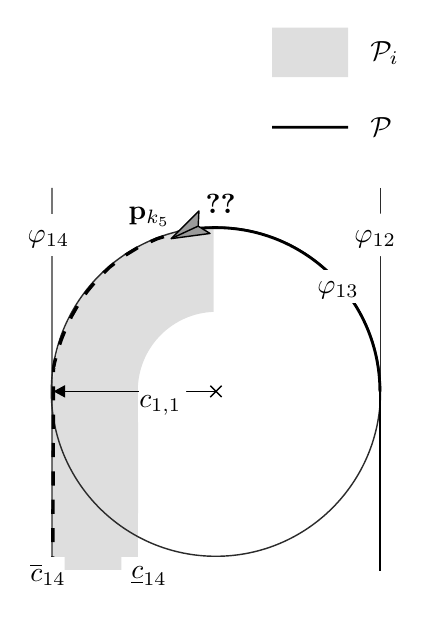
\begin{tikzpicture}[y=0.80pt, x=0.80pt, yscale=-1.2*\globalscale, xscale=1.2*\globalscale, inner sep=0pt, outer sep=0pt]



\path[draw=c2B2B2B,line join=round,line width=0.512pt] (137.9100,95.3391) -- (137.9100,239.5120);



  \path[fill=cFFFFFF,line join=round,line width=0.160pt] (144.6860,105.0630) -- (131.2360,105.0630) -- (131.2360,121.0330) -- (144.6960,121.0670) -- (144.6860,105.0630) -- cycle;



  \path[cm={{1.0,0.0,0.0,1.0,(128.0,118.0)}}] (0.0000,0.0000) node[above right] () {$\varphi_{12}$};



\path[fill=cDEDEDE,line join=round,line width=0.160pt] (14.4062,169.9360) -- (14.4311,169.9360) .. controls (15.3584,137.0320) and (42.0351,110.5710) .. (75.0243,109.9900) -- (75.0243,142.0480) .. controls (59.7109,142.6110) and (47.3600,154.7750) .. (46.5019,170.0120) -- (46.5148,182.6390) -- (46.5019,182.9250) -- (46.5019,183.2150) .. controls (46.5154,183.9430) and (46.6203,184.7000) .. (46.6001,185.4160) -- (46.6055,185.4230) -- (46.6055,187.1950) -- (46.5019,227.3090) -- (46.5019,234.5270) -- (46.4833,234.5270) -- (46.4830,234.6700) -- (46.4723,235.4800) -- (46.5303,239.1710) -- (14.2304,239.1780) .. controls (14.2304,237.5050) and (14.2092,240.8130) .. (14.1991,237.1110) -- (14.1991,235.5690) -- (14.1991,235.2560) -- (14.1991,234.8370) -- (14.1991,234.5320) -- (14.1991,171.8980) -- (14.4062,169.9360) -- cycle;



\path[draw=c2B2B2B,line join=round,line width=0.512pt] (75.8516,172.0930) ellipse (1.7421cm and 1.7421cm);



\path[draw=black,line join=round,line width=0.512pt] (78.0152,174.1270) -- (73.7395,169.8460);



\path[draw=black,line join=round,line width=0.512pt] (73.7417,174.1270) -- (78.0230,169.8460);



\path[draw=c2B2B2B,line join=round,line width=0.512pt] (14.1483,95.3578) -- (14.1477,239.5310);



\path[draw=black,line join=round,line width=0.512pt] (75.9234,172.0190) -- (14.0743,172.0190);



\path[fill=black,line join=round,line width=0.160pt] (19.0789,174.3350) -- (19.0727,169.6190) -- (14.7563,171.9820) -- (19.0789,174.3350) -- cycle;



  \path[fill=cFFFFFF,line join=round,line width=0.160pt,rounded corners=0.0000cm] (8.0901,105.0980) rectangle (20.5396,121.0676);



  \path[cm={{1.0,0.0,0.0,1.0,(5.0,118.0)}}] (0.0000,0.0000) node[above right] () {$\varphi_{14}$};



\path[draw=black,line join=round,line width=1.024pt] (67.5256,111.0380) .. controls (69.2504,110.2990) and (75.8630,110.3510) .. (75.8630,110.3510) .. controls (109.9540,110.3510) and (137.5900,137.9880) .. (137.5900,172.0790);



  \path[fill=cFFFFFF,line join=round,line width=0.160pt,rounded corners=0.0000cm] (115.2640,126.2090) rectangle (131.2335,138.6585);



  \path[cm={{1.0,0.0,0.0,1.0,(114.0,137.0)}}] (0.0000,0.0000) node[above right] () {$\varphi_{13}$};



  \path[fill=cFFFFFF,line join=round,line width=0.160pt] (52.6996,234.3410) -- (40.2501,234.3410) -- (40.2318,246.3700) -- (52.7105,246.3700) -- (52.6996,234.3410) -- cycle;



  \path[cm={{1.0,0.0,0.0,1.0,(44.0,245.0)}}] (0.0000,0.0000) node[above right] () {$\underline{c}_{14}$};



  \path[fill=cFFFFFF,line join=round,line width=0.160pt] (64.6687,169.3940) -- (46.9391,169.3930) -- (46.9391,181.8430) -- (64.6687,181.8430) -- (64.6687,169.3940) -- cycle;



  \path[cm={{1.0,0.0,0.0,1.0,(47.0,181.0)}}] (0.0000,0.0000) node[above right] () {$c_{1,1}$};



\path[fill=black,line join=round,line width=0.256pt] (13.8207,228.7410) -- (13.8435,223.4080) -- (15.1234,223.4140) -- (15.1007,228.7470) -- (13.8207,228.7410) -- cycle(13.8662,218.0750) -- (13.8890,212.7420) -- (15.1690,212.7470) -- (15.1462,218.0800) -- (13.8662,218.0750) -- cycle(13.9117,207.4080) -- (13.9345,202.0750) -- (15.2145,202.0800) -- (15.1917,207.4140) -- (13.9117,207.4080) -- cycle(13.9572,196.7420) -- (13.9800,191.4080) -- (15.2600,191.4140) -- (15.2372,196.7470) -- (13.9572,196.7420) -- cycle(14.0028,186.0750) -- (14.0255,180.7420) -- (15.3055,180.7470) -- (15.2828,186.0810) -- (14.0028,186.0750) -- cycle(14.0483,175.4090) -- (14.0711,170.0750) -- (15.3510,170.0810) -- (15.3283,175.4140) -- (14.0483,175.4090) -- cycle(14.0938,164.7420) -- (14.1004,163.1940) -- (14.1116,163.0700) -- (14.1481,162.9500) -- (14.2078,162.8390) -- (14.2888,162.7440) -- (14.3849,162.6630) -- (14.4954,162.6040) -- (14.6155,162.5680) -- (14.7404,162.5570) -- (14.1975,162.5580) -- (14.4982,161.0400) -- (14.8987,159.3600) -- (16.1499,159.6300) -- (15.7494,161.3100) -- (15.4579,162.7820) -- (14.7404,163.8370) -- (15.3804,163.2000) -- (15.3738,164.7470) -- (14.0938,164.7420) -- cycle(16.4171,154.1910) -- (17.1786,151.9470) -- (18.2993,149.1670) -- (19.5002,149.6100) -- (18.3795,152.3900) -- (17.6397,154.5700) -- (16.4171,154.1910) -- cycle(20.5366,144.2860) -- (20.9681,143.3850) -- (23.1393,139.5830) -- (24.2741,140.1750) -- (22.1029,143.9770) -- (21.7089,144.7990) -- (20.5366,144.2860) -- cycle(26.1128,135.1000) -- (26.8488,134.0250) -- (29.4547,130.8780) -- (30.4785,131.6470) -- (27.8725,134.7930) -- (27.1990,135.7770) -- (26.1128,135.1000) -- cycle(33.1525,126.9590) -- (35.2417,124.9010) -- (37.1822,123.3740) -- (38.0303,124.3330) -- (36.0897,125.8600) -- (34.0975,127.8220) -- (33.1525,126.9590) -- cycle(41.5104,120.1440) -- (46.0624,117.3650) -- (46.7947,118.4150) -- (42.2427,121.1940) -- (41.5104,120.1440) -- cycle(50.9592,115.0720) -- (53.4451,113.9480) -- (56.0106,113.1560) -- (56.4648,114.3530) -- (53.8993,115.1450) -- (51.5589,116.2030) -- (50.9592,115.0720) -- cycle(61.1063,111.5820) -- (61.2085,111.5500) -- (66.4314,110.6160) -- (66.7338,111.8590) -- (61.5109,112.7940) -- (61.5606,112.7790) -- (61.1063,111.5820) -- cycle(13.7752,239.4080) -- (13.7979,234.0750) -- (15.0779,234.0800) -- (15.0552,239.4130) -- (13.7752,239.4080) -- cycle;



\path[cm={{1.0,0.0,0.0,1.0,(43.0,110.0)}}] (0.0000,0.0000) node[above right] () {$\mathbf{p}_{k_5}$};

\path[cm={{1.0,0.0,0.0,1.0,(72.0,105.0)}}] (0.0000,0.0000) node[above right] () {\ref{sth:i}};

  \path[fill=cFFFFFF,line join=round,line width=0.160pt] (18.9147,234.3410) -- (6.4652,234.3410) -- (6.4316,246.4160) -- (18.9102,246.3850) -- (18.9147,234.3410) -- cycle;



  \path[cm={{1.0,0.0,0.0,1.0,(6.0,245.0)}}] (0.0000,0.0000) node[above right] () {$\overline{c}_{14}$};



\path[draw=black,fill=c9B9B9B,line join=round,line width=0.512pt] (58.9895,114.4960) -- (73.6370,112.5410) -- (69.1896,109.7900) -- (69.4587,104.0670) -- (58.9895,114.4960) -- cycle;



\path[draw=black,line join=round,line width=0.512pt] (59.2931,114.3470) -- (69.0932,109.8070);



\path[draw=black,line join=round,line width=1.024pt] (137.5900,239.4500) -- (137.5900,171.8800);



\path[fill=cDEDEDE,line join=round,even odd rule,line width=0.160pt] (97.0260,35.0828) -- (125.6100,35.0831) -- (125.6100,53.6677) -- (97.0260,53.6675) -- (97.0260,35.0828) -- cycle;



\path[cm={{1.0,0.0,0.0,1.0,(134.0,49.0)}}] (0.0000,0.0000) node[above right] () {$\mathcal{P}_i$};



\path[draw=black,line join=round,line width=1.024pt] (97.0260,72.5827) -- (125.6110,72.5829);



\path[cm={{1.0,0.0,0.0,1.0,(134.0,76.0)}}] (0.0000,0.0000) node[above right] () {$\mathcal{P}$};


\end{tikzpicture}


  \caption[Path of a UAV flying a given stage]{.}
  \label{fig:tee1}
\end{figure}
\begin{figure}[h]
  \centering
  
\definecolor{c2B2B2B}{RGB}{43,43,43}
\definecolor{cDEDEDE}{RGB}{222,222,222}
\definecolor{c989898}{RGB}{152,152,152}
\definecolor{cFFFFFF}{RGB}{255,255,255}
\definecolor{c4D4D4D}{RGB}{77,77,77}
\definecolor{c9B9B9B}{RGB}{155,155,155}


\def \globalscale {1.000000}
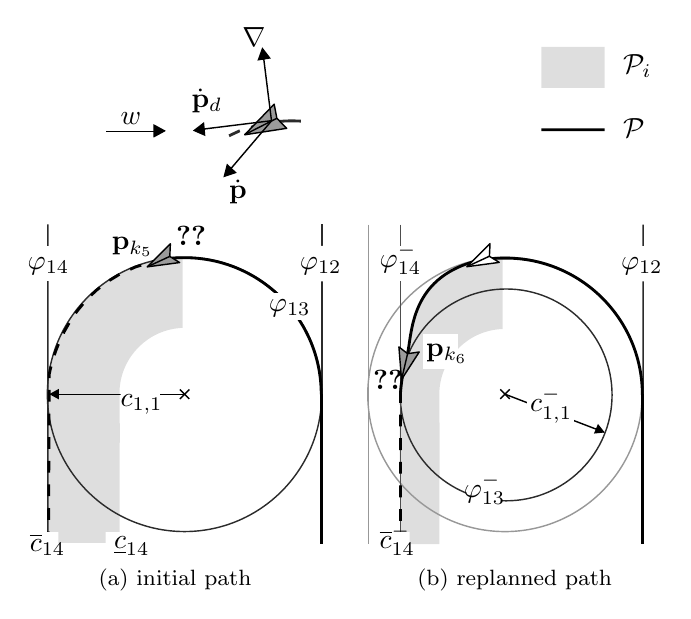
\begin{tikzpicture}[y=0.80pt, x=0.80pt, yscale=-\globalscale, xscale=\globalscale, inner sep=0pt, outer sep=0pt]
\path[fill=c2B2B2B,line join=round,line width=0.256pt] (101.0350,53.6179) -- (96.2027,55.8748) -- (95.7468,54.6788) -- (100.5790,52.4218) -- (101.0350,53.6179) -- cycle(111.1420,50.5445) -- (106.0290,52.0626) -- (105.7610,50.8111) -- (110.8730,49.2930) -- (111.1420,50.5445) -- cycle;



\path[draw=c2B2B2B,line join=round,line width=1.024pt] (128.3820,48.6757) .. controls (127.0480,48.5917) and (125.7060,48.5494) .. (124.3560,48.5494) .. controls (119.7720,48.5494) and (115.2670,49.0390) .. (110.8680,49.9835);



  \path[fill=cDEDEDE,line join=round,even odd rule,line width=0.160pt] (201.2220,113.9290) .. controls (207.0530,111.9750) and (213.0250,110.6150) .. (219.4860,110.5010) -- (219.4860,142.5600) .. controls (204.1730,143.1220) and (191.8220,155.2870) .. (190.9640,170.5230) -- (190.9770,183.1500) -- (190.9640,183.4360) -- (190.9640,183.7260) .. controls (190.9770,184.4540) and (191.0820,185.2110) .. (191.0620,185.9270) -- (191.0670,185.9340) -- (191.0670,187.7060) -- (190.9640,227.8200) -- (190.9640,235.0380) -- (190.9450,235.0380) -- (190.9450,235.1810) -- (190.9340,235.9910) -- (190.9920,239.6820) -- (173.2000,239.6860) .. controls (173.4790,219.6570) and (172.4790,191.1610) .. (173.3370,172.5260) .. controls (173.7560,163.4250) and (175.7760,156.4540) .. (176.3670,154.3980) .. controls (178.5870,146.6790) and (177.0030,123.9390) .. (200.7770,114.0980) -- (201.2220,113.9290) -- cycle;



  \path[draw=c989898,line join=round,line width=0.512pt] (220.5790,172.1070) ellipse (1.7421cm and 1.7421cm);



  \path[draw=black,line join=round,line width=0.512pt] (222.7480,174.1440) -- (218.4670,169.8620);



  \path[draw=c2B2B2B,line join=round,line width=0.512pt] (283.0110,95.4499) -- (283.0100,239.6230);



  \path[draw=black,line join=round,line width=1.024pt] (212.5660,111.2220) .. controls (214.2910,110.4830) and (220.9040,110.5350) .. (220.9040,110.5350) .. controls (254.9950,110.5350) and (282.6310,138.1720) .. (282.6310,172.2630);



  \path[draw=black,line join=round,line width=0.512pt] (218.4680,174.1410) -- (222.7490,169.8600);



    \path[fill=cFFFFFF,line join=round,line width=0.160pt] (289.4020,105.0980) -- (276.9530,105.0980) -- (276.9530,121.0670) -- (289.4080,121.0670) -- (289.4020,105.0980) -- cycle;



    \path[cm={{1.0,0.0,0.0,1.0,(273.0,118.0)}}] (0.0000,0.0000) node[above right] () {$\varphi_{12}$};



  \path[draw=black,line join=round,line width=1.024pt] (282.6300,239.6340) -- (282.6300,172.0640);



  \path[draw=c2B2B2B,line join=round,line width=0.512pt] (221.1170,172.3260) ellipse (1.3451cm and 1.3451cm);



  \path[draw=c4D4D4D,line join=round,line width=0.512pt] (173.4260,95.3725) -- (173.4260,239.5460);



  \path[draw=black,line join=round,line width=0.512pt] (265.2780,189.1390) -- (220.7780,172.0720);



  \path[draw=black,line join=round,line width=1.024pt] (212.0450,110.8620) .. controls (176.5020,117.4390) and (178.8960,145.6300) .. (176.3720,154.4050) .. controls (173.7630,163.4760) and (173.3650,171.9460) .. (173.3650,171.9460) -- (173.3790,172.2110) -- (173.4210,172.6590);



  \path[draw=black,fill=c9B9B9B,line join=round,line width=0.512pt] (173.8510,165.3770) -- (181.8430,152.9480) -- (176.6230,153.7110) -- (172.6800,150.6460) -- (173.8510,165.3770) -- cycle;



  \path[fill=black,line join=round,line width=0.256pt] (172.7330,229.2390) -- (172.7330,223.9060) -- (174.0130,223.9060) -- (174.0130,229.2390) -- (172.7330,229.2390) -- cycle(172.7330,218.5730) -- (172.7330,213.2390) -- (174.0130,213.2390) -- (174.0130,218.5730) -- (172.7330,218.5730) -- cycle(172.7330,207.9060) -- (172.7330,202.5730) -- (174.0130,202.5730) -- (174.0130,207.9060) -- (172.7330,207.9060) -- cycle(172.7330,197.2390) -- (172.7330,191.9060) -- (174.0130,191.9060) -- (174.0130,197.2390) -- (172.7330,197.2390) -- cycle(172.7330,186.5730) -- (172.7330,181.2390) -- (174.0130,181.2390) -- (174.0130,186.5730) -- (172.7330,186.5730) -- cycle(172.7330,175.9060) -- (172.7330,172.3360) -- (174.0130,172.3360) -- (174.0130,175.9060) -- (172.7330,175.9060) -- cycle(172.7330,239.9060) -- (172.7330,234.5730) -- (174.0130,234.5730) -- (174.0130,239.9060) -- (172.7330,239.9060) -- cycle;



    \path[fill=cFFFFFF,line join=round,line width=0.160pt,rounded corners=0.0000cm] (167.3680,105.0980) rectangle (179.8176,121.0676);



    \path[cm={{1.0,0.0,0.0,1.0,(164.0,118.0)}}] (0.0000,0.0000) node[above right] () {$\varphi_{14}^-$};



    \path[fill=cFFFFFF,line join=round,line width=0.160pt] (177.5750,234.3400) -- (165.1260,234.3400) -- (165.0920,246.4150) -- (177.5710,246.3840) -- (177.5750,234.3400) -- cycle;



    \path[cm={{1.0,0.0,0.0,1.0,(164.0,245.0)}}] (0.0000,0.0000) node[above right] () {$\overline{c}_{14}^-$};



    \path[fill=cFFFFFF,line join=round,line width=0.160pt,rounded corners=0.0000cm] (230.3230,173.2320) rectangle (251.5725,189.2016);



    \path[cm={{1.0,0.0,0.0,1.0,(232.0,185.0)}}] (0.0000,0.0000) node[above right] () {$c_{1,1}^-$};



  \path[draw=black,fill=cFFFFFF,line join=round,line width=0.512pt] (203.3560,114.4210) -- (218.0050,112.4770) -- (213.5600,109.7230) -- (213.8340,104.0000) -- (203.3560,114.4210) -- cycle;



    \path[fill=cFFFFFF,line join=round,line width=0.160pt] (199.4770,144.8830) -- (183.5080,144.8830) -- (183.5080,160.8530) -- (199.4770,160.8530) -- (199.4770,144.8830) -- cycle;



    \path[cm={{1.0,0.0,0.0,1.0,(185.0,158.0)}}] (0.0000,0.0000) node[above right] () {$\mathbf{p}_{k_6}$};

    \path[cm={{1.0,0.0,0.0,1.0,(161.0,170.0)}}] (0.0000,0.0000) node[above right] () {\ref{sth:iii}};

    \path[fill=cFFFFFF,line join=round,line width=0.160pt,rounded corners=0.0000cm] (192.4050,96.8819) rectangle (204.8546,109.3314);


  \path[draw=black,line join=round,line width=0.512pt] (203.7170,114.2570) -- (213.5160,109.7120);



  \path[draw=black,line join=round,line width=0.512pt] (174.0250,164.7330) -- (176.5840,153.7760);



    \path[fill=cFFFFFF,line join=round,line width=0.160pt] (219.2260,208.5700) -- (203.2560,208.5700) -- (203.2560,224.5400) -- (219.2260,224.5390) -- (219.2260,208.5700) -- cycle;



    \path[cm={{1.0,0.0,0.0,1.0,(202.0,222.0)}}] (0.0000,0.0000) node[above right] () {$\varphi_{13}^-$};



  \path[draw=c989898,line join=round,line width=0.512pt] (158.8570,95.3893) -- (158.8570,239.5620);



  \path[cm={{1.0,0.0,0.0,1.0,(181.0,261.0)}}] (0.0000,0.0000) node[above right] () {\footnotesize (b) replanned path};



  \path[fill=black,line join=round,line width=0.160pt] (262.5930,185.4440) -- (260.7610,189.7900) -- (265.6570,189.2950) -- (262.5930,185.4440) -- cycle;



\path[draw=c2B2B2B,line join=round,line width=0.512pt] (137.9100,95.3391) -- (137.9100,239.5120);



  \path[fill=cFFFFFF,line join=round,line width=0.160pt] (144.6860,105.0630) -- (131.2360,105.0630) -- (131.2360,121.0330) -- (144.6960,121.0670) -- (144.6860,105.0630) -- cycle;



  \path[cm={{1.0,0.0,0.0,1.0,(128.0,118.0)}}] (0.0000,0.0000) node[above right] () {$\varphi_{12}$};



\path[fill=cDEDEDE,line join=round,line width=0.160pt] (14.4062,169.9360) -- (14.4311,169.9360) .. controls (15.3584,137.0320) and (42.0351,110.5710) .. (75.0243,109.9900) -- (75.0243,142.0480) .. controls (59.7109,142.6110) and (47.3600,154.7750) .. (46.5019,170.0120) -- (46.5148,182.6390) -- (46.5019,182.9250) -- (46.5019,183.2150) .. controls (46.5154,183.9430) and (46.6203,184.7000) .. (46.6001,185.4160) -- (46.6055,185.4230) -- (46.6055,187.1950) -- (46.5019,227.3090) -- (46.5019,234.5270) -- (46.4833,234.5270) -- (46.4830,234.6700) -- (46.4723,235.4800) -- (46.5303,239.1710) -- (14.2304,239.1780) .. controls (14.2304,237.5050) and (14.2092,240.8130) .. (14.1991,237.1110) -- (14.1991,235.5690) -- (14.1991,235.2560) -- (14.1991,234.8370) -- (14.1991,234.5320) -- (14.1991,171.8980) -- (14.4062,169.9360) -- cycle;



\path[draw=c2B2B2B,line join=round,line width=0.512pt] (75.8516,172.0930) ellipse (1.7421cm and 1.7421cm);



\path[draw=black,line join=round,line width=0.512pt] (78.0152,174.1270) -- (73.7395,169.8460);



\path[draw=black,line join=round,line width=0.512pt] (73.7417,174.1270) -- (78.0230,169.8460);



\path[draw=c2B2B2B,line join=round,line width=0.512pt] (14.1483,95.3578) -- (14.1477,239.5310);



\path[draw=black,line join=round,line width=0.512pt] (75.9234,172.0190) -- (14.0743,172.0190);



\path[fill=black,line join=round,line width=0.160pt] (19.0789,174.3350) -- (19.0727,169.6190) -- (14.7563,171.9820) -- (19.0789,174.3350) -- cycle;



  \path[fill=cFFFFFF,line join=round,line width=0.160pt,rounded corners=0.0000cm] (8.0901,105.0980) rectangle (20.5396,121.0676);



  \path[cm={{1.0,0.0,0.0,1.0,(5.0,118.0)}}] (0.0000,0.0000) node[above right] () {$\varphi_{14}$};



\path[draw=black,line join=round,line width=1.024pt] (67.5256,111.0380) .. controls (69.2504,110.2990) and (75.8630,110.3510) .. (75.8630,110.3510) .. controls (109.9540,110.3510) and (137.5900,137.9880) .. (137.5900,172.0790);



  \path[fill=cFFFFFF,line join=round,line width=0.160pt,rounded corners=0.0000cm] (115.2640,126.2090) rectangle (131.2335,138.6585);



  \path[cm={{1.0,0.0,0.0,1.0,(114.0,137.0)}}] (0.0000,0.0000) node[above right] () {$\varphi_{13}$};



  \path[fill=cFFFFFF,line join=round,line width=0.160pt] (52.6996,234.3410) -- (40.2501,234.3410) -- (40.2318,246.3700) -- (52.7105,246.3700) -- (52.6996,234.3410) -- cycle;



  \path[cm={{1.0,0.0,0.0,1.0,(44.0,245.0)}}] (0.0000,0.0000) node[above right] () {$\underline{c}_{14}$};



  \path[fill=cFFFFFF,line join=round,line width=0.160pt] (64.6687,169.3940) -- (46.9391,169.3930) -- (46.9391,181.8430) -- (64.6687,181.8430) -- (64.6687,169.3940) -- cycle;



  \path[cm={{1.0,0.0,0.0,1.0,(47.0,181.0)}}] (0.0000,0.0000) node[above right] () {$c_{1,1}$};



\path[fill=black,line join=round,line width=0.256pt] (13.8207,228.7410) -- (13.8435,223.4080) -- (15.1234,223.4140) -- (15.1007,228.7470) -- (13.8207,228.7410) -- cycle(13.8662,218.0750) -- (13.8890,212.7420) -- (15.1690,212.7470) -- (15.1462,218.0800) -- (13.8662,218.0750) -- cycle(13.9117,207.4080) -- (13.9345,202.0750) -- (15.2145,202.0800) -- (15.1917,207.4140) -- (13.9117,207.4080) -- cycle(13.9572,196.7420) -- (13.9800,191.4080) -- (15.2600,191.4140) -- (15.2372,196.7470) -- (13.9572,196.7420) -- cycle(14.0028,186.0750) -- (14.0255,180.7420) -- (15.3055,180.7470) -- (15.2828,186.0810) -- (14.0028,186.0750) -- cycle(14.0483,175.4090) -- (14.0711,170.0750) -- (15.3510,170.0810) -- (15.3283,175.4140) -- (14.0483,175.4090) -- cycle(14.0938,164.7420) -- (14.1004,163.1940) -- (14.1116,163.0700) -- (14.1481,162.9500) -- (14.2078,162.8390) -- (14.2888,162.7440) -- (14.3849,162.6630) -- (14.4954,162.6040) -- (14.6155,162.5680) -- (14.7404,162.5570) -- (14.1975,162.5580) -- (14.4982,161.0400) -- (14.8987,159.3600) -- (16.1499,159.6300) -- (15.7494,161.3100) -- (15.4579,162.7820) -- (14.7404,163.8370) -- (15.3804,163.2000) -- (15.3738,164.7470) -- (14.0938,164.7420) -- cycle(16.4171,154.1910) -- (17.1786,151.9470) -- (18.2993,149.1670) -- (19.5002,149.6100) -- (18.3795,152.3900) -- (17.6397,154.5700) -- (16.4171,154.1910) -- cycle(20.5366,144.2860) -- (20.9681,143.3850) -- (23.1393,139.5830) -- (24.2741,140.1750) -- (22.1029,143.9770) -- (21.7089,144.7990) -- (20.5366,144.2860) -- cycle(26.1128,135.1000) -- (26.8488,134.0250) -- (29.4547,130.8780) -- (30.4785,131.6470) -- (27.8725,134.7930) -- (27.1990,135.7770) -- (26.1128,135.1000) -- cycle(33.1525,126.9590) -- (35.2417,124.9010) -- (37.1822,123.3740) -- (38.0303,124.3330) -- (36.0897,125.8600) -- (34.0975,127.8220) -- (33.1525,126.9590) -- cycle(41.5104,120.1440) -- (46.0624,117.3650) -- (46.7947,118.4150) -- (42.2427,121.1940) -- (41.5104,120.1440) -- cycle(50.9592,115.0720) -- (53.4451,113.9480) -- (56.0106,113.1560) -- (56.4648,114.3530) -- (53.8993,115.1450) -- (51.5589,116.2030) -- (50.9592,115.0720) -- cycle(61.1063,111.5820) -- (61.2085,111.5500) -- (66.4314,110.6160) -- (66.7338,111.8590) -- (61.5109,112.7940) -- (61.5606,112.7790) -- (61.1063,111.5820) -- cycle(13.7752,239.4080) -- (13.7979,234.0750) -- (15.0779,234.0800) -- (15.0552,239.4130) -- (13.7752,239.4080) -- cycle;



\path[cm={{1.0,0.0,0.0,1.0,(43.0,110.0)}}] (0.0000,0.0000) node[above right] () {$\mathbf{p}_{k_5}$};

\path[cm={{1.0,0.0,0.0,1.0,(72.0,105.0)}}] (0.0000,0.0000) node[above right] () {\ref{sth:i}};

  \path[fill=cFFFFFF,line join=round,line width=0.160pt] (18.9147,234.3410) -- (6.4652,234.3410) -- (6.4316,246.4160) -- (18.9102,246.3850) -- (18.9147,234.3410) -- cycle;



  \path[cm={{1.0,0.0,0.0,1.0,(6.0,245.0)}}] (0.0000,0.0000) node[above right] () {$\overline{c}_{14}$};



\path[draw=black,fill=c9B9B9B,line join=round,line width=0.512pt] (58.9895,114.4960) -- (73.6370,112.5410) -- (69.1896,109.7900) -- (69.4587,104.0670) -- (58.9895,114.4960) -- cycle;



\path[draw=black,line join=round,line width=0.512pt] (59.2931,114.3470) -- (69.0932,109.8070);



\path[cm={{1.0,0.0,0.0,1.0,(37.0,261.0)}}] (0.0000,0.0000) node[above right] () {\footnotesize (a) initial path};



\path[draw=black,line join=round,line width=1.024pt] (137.5900,239.4500) -- (137.5900,171.8800);



\path[fill=cDEDEDE,line join=round,even odd rule,line width=0.160pt] (237.0260,15.0828) -- (265.6100,15.0831) -- (265.6100,33.6677) -- (237.0260,33.6675) -- (237.0260,15.0828) -- cycle;



\path[cm={{1.0,0.0,0.0,1.0,(274.0,29.0)}}] (0.0000,0.0000) node[above right] () {$\mathcal{P}_i$};



\path[draw=black,line join=round,line width=1.024pt] (237.0260,52.5827) -- (265.6110,52.5829);



\path[cm={{1.0,0.0,0.0,1.0,(274.0,56.0)}}] (0.0000,0.0000) node[above right] () {$\mathcal{P}$};



\path[draw=black,fill=c9B9B9B,line join=round,line width=0.512pt] (103.0020,54.8369) -- (121.9910,51.9150) -- (117.5520,47.3939) -- (116.3400,41.0080) -- (103.0020,54.8369) -- cycle;



\path[draw=black,line join=round,line width=0.512pt] (115.1520,48.6445) -- (111.3670,18.4898);



\path[draw=black,line join=round,line width=0.512pt] (115.2340,48.4465) -- (94.3696,72.9709);



\path[cm={{1.0,0.0,0.0,1.0,(102.0,15.0)}}] (0.0000,0.0000) node[above right] () {$\nabla\varPhi$};



\path[cm={{1.0,0.0,0.0,1.0,(96.0,86.0)}}] (0.0000,0.0000) node[above right] () {$\dot{\mathbf{p}}$};



\path[cm={{1.0,0.0,0.0,1.0,(79.0,45.0)}}] (0.0000,0.0000) node[above right] () {$\dot{\mathbf{p}}_d$};



\path[draw=black,line join=round,line width=0.512pt] (117.5520,47.3796) -- (103.1340,54.7265);



\path[fill=black,line join=round,line width=0.160pt] (99.4724,72.0401) -- (94.9925,67.8546) -- (93.3980,74.0506) -- (99.4724,72.0401) -- cycle;



\path[fill=black,line join=round,line width=0.160pt] (108.7830,21.3255) -- (114.8390,20.3742) -- (110.9400,15.3018) -- (108.7830,21.3255) -- cycle;



\path[fill=black,line join=round,line width=0.160pt] (79.6380,52.9767) -- (85.2585,55.4260) -- (84.6922,49.0532) -- (79.6380,52.9767) -- cycle;



\path[draw=black,line join=round,line width=0.512pt] (82.5181,52.4879) -- (114.8620,48.5042);



\path[draw=black,line join=round,line width=0.512pt] (40.3847,53.3572) -- (62.7169,53.3572);



\path[cm={{1.0,0.0,0.0,1.0,(47.0,50.0)}}] (0.0000,0.0000) node[above right] () {$w$};



\path[fill=black,line join=round,line width=0.160pt] (61.8249,50.0137) -- (61.8330,56.1447) -- (67.4450,53.0723) -- (61.8249,50.0137) -- cycle;




\end{tikzpicture}


  \caption[Alteration of the path parameter]{The alteration of the path parameter $c_{1,1}$, the radius of the circle.}
  \label{fig:tee1}
\end{figure}

\begin{figure}[h]
  \centering
  
\definecolor{c2B2B2B}{RGB}{43,43,43}
\definecolor{cDEDEDE}{RGB}{222,222,222}
\definecolor{c989898}{RGB}{152,152,152}
\definecolor{cFFFFFF}{RGB}{255,255,255}
\definecolor{c4D4D4D}{RGB}{77,77,77}
\definecolor{c9B9B9B}{RGB}{155,155,155}


\def \globalscale {1.000000}
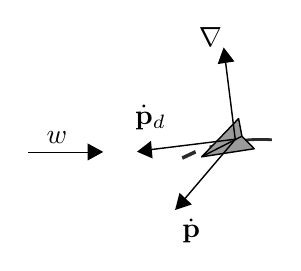
\begin{tikzpicture}[y=0.80pt, x=0.80pt, yscale=-1.25*\globalscale, xscale=1.25*\globalscale, inner sep=0pt, outer sep=0pt]
\path[fill=c2B2B2B,line join=round,line width=0.256pt] (101.0350,53.6179) -- (96.2027,55.8748) -- (95.7468,54.6788) -- (100.5790,52.4218) -- (101.0350,53.6179) -- cycle(111.1420,50.5445) -- (106.0290,52.0626) -- (105.7610,50.8111) -- (110.8730,49.2930) -- (111.1420,50.5445) -- cycle;



\path[draw=c2B2B2B,line join=round,line width=1.024pt] (128.3820,48.6757) .. controls (127.0480,48.5917) and (125.7060,48.5494) .. (124.3560,48.5494) .. controls (119.7720,48.5494) and (115.2670,49.0390) .. (110.8680,49.9835);





\path[draw=black,fill=c9B9B9B,line join=round,line width=0.512pt] (103.0020,54.8369) -- (121.9910,51.9150) -- (117.5520,47.3939) -- (116.3400,41.0080) -- (103.0020,54.8369) -- cycle;



\path[draw=black,line join=round,line width=0.512pt] (115.1520,48.6445) -- (111.3670,18.4898);



\path[draw=black,line join=round,line width=0.512pt] (115.2340,48.4465) -- (94.3696,72.9709);



\path[cm={{1.0,0.0,0.0,1.0,(102.0,15.0)}}] (0.0000,0.0000) node[above right] () {$\nabla\varPhi$};



\path[cm={{1.0,0.0,0.0,1.0,(96.0,86.0)}}] (0.0000,0.0000) node[above right] () {$\dot{\mathbf{p}}$};



\path[cm={{1.0,0.0,0.0,1.0,(79.0,45.0)}}] (0.0000,0.0000) node[above right] () {$\dot{\mathbf{p}}_d$};



\path[draw=black,line join=round,line width=0.512pt] (117.5520,47.3796) -- (103.1340,54.7265);



\path[fill=black,line join=round,line width=0.160pt] (99.4724,72.0401) -- (94.9925,67.8546) -- (93.3980,74.0506) -- (99.4724,72.0401) -- cycle;



\path[fill=black,line join=round,line width=0.160pt] (108.7830,21.3255) -- (114.8390,20.3742) -- (110.9400,15.3018) -- (108.7830,21.3255) -- cycle;



\path[fill=black,line join=round,line width=0.160pt] (79.6380,52.9767) -- (85.2585,55.4260) -- (84.6922,49.0532) -- (79.6380,52.9767) -- cycle;



\path[draw=black,line join=round,line width=0.512pt] (82.5181,52.4879) -- (114.8620,48.5042);



\path[draw=black,line join=round,line width=0.512pt] (40.3847,53.3572) -- (62.7169,53.3572);



\path[cm={{1.0,0.0,0.0,1.0,(47.0,50.0)}}] (0.0000,0.0000) node[above right] () {$w$};



\path[fill=black,line join=round,line width=0.160pt] (61.8249,50.0137) -- (61.8330,56.1447) -- (67.4450,53.0723) -- (61.8249,50.0137) -- cycle;


\end{tikzpicture}


  \caption[External interference on the path]{.}
  \label{fig:tee1}
\end{figure}

%Equation~(\ref{eq:state-control}) accounts for the energy due to the change of parameters $\mathbf{u}_k-\mathbf{u}_{k-1}$. For instance, when the trajectory $\varphi_1$ is a circle (see Figure~\ref{fig:tee1}), a decrement in the trajectory parameter $c_{1,1}$--the radius of the circle--adds a negative contribution. It thus simulates the lowering of instantaneous energy consumption ($\nu_{1,1}c_{1,1}>\nu_{1,1}c_{1,1}^-$) for a given $\nu_{1,1}$, that is then summed to the first coefficient $\alpha_0$ in Equation~(\ref{eq:state-details}), shifting the modeled energy.

The set
\begin{equation}\label{eq:area}
  \mathcal{P}_i:=\{\mathbf{p}_k\mid\varphi_i(\mathbf{p}_k,c_{i}^\rho)\in\mathcal{C}_i\},
\end{equation}
delimits the area where the $i$-th path $\varphi_i$ is free to evolve using the path parameters $c_i^\rho$ (the gray area in \fref{fig:tee1}{Figure}). $\varphi_i$ is a function of the two coordinates and the path parameters, and is equal to zero when a point $\mathbf{p}_k$ is on the path. Physically, this means the UAV is flying exactly over the nominal trajectory. 

The path parameters allows to change the path. They are a way to alter the nominal trajectory in the initial plan and thus alter the energy by changing the flying time in the example in \fref{fig:il-abs}{Figure}.
In fact, the algorithm uses the set from \frefeq{eq:area} to find the path parameters such that the plan consisting of flying $\varphi_i$ has the highest energy, while still respecting the constraints. In \fref{fig:tee1}{Figure}, the parameter radius of the circle $c_{1,1}$ is replanned as, e.g., averse atmospheric conditions do not allow to terminate the plan.

We derive the new position $\mathbf{p}_{k+1}$ computing the vector field 
\begin{equation}
  \nabla\varphi_i:=\begin{bmatrix}\partial\varphi_i/\partial x \\ \partial\varphi_i/\partial y\end{bmatrix},  
\end{equation}
and the direction to follow in the form of velocity vector~\cite{de2017guidance}
\begin{equation}\label{eq:pd}
  \dot{\mathbf{p}}_d(\mathbf{p}_k):=E\nabla\varphi_i-k_e\varphi_i\nabla\varphi_i,
\end{equation}
where $E$ specifies the rotation (it influence the tracking direction). For instance
\begin{equation}
  E=\begin{bmatrix}
    0&1\\-1&0
  \end{bmatrix},
\end{equation}
is the counter clockwise direction, $-E$ the clockwise direction. 

$k_e\in\mathbb{R}_{\geq 0}$ is the gain to adjusts the speed of convergence. The direction the velocity vector $\dot{\mathbf{p}}_d$ is pointing at is generally different from the course heading $\dot{\mathbf{p}}$ due to the atmospheric interferences (wind $w\in\mathbb{R}$ in the top of \fref{fig:tee1}{Figure}).

The scaling factors for the path parameters from \frefeq{eq:state-control} are derived empirically. For the example in \fref{fig:tee1}{Figure}, we can obtain the scaling factor $\nu_{1,1}$ measuring the time needed to compute the path with the lowest configuration $\underline{c}_1$, $\underline{t}$ and the highest $\overline{t}$. 

The variation of the control hence results in an approximate measure of the plans' time variation with factors
\begin{equation}\label{eq:scale-traj}\begin{split}
  \nu_{i,j}&=\left((\overline{t}-\underline{t})/(\overline{c}_{i,j}-\underline{c}_{i,j})\right)/\rho,\\
  \tau_{i,j}&=\left(\underline{c}_{i,j}(\underline{t}-\overline{t})/(\overline{c}_{i,j}-\underline{c}_{i,j})+\underline{t}\right)/\rho,
\end{split}\end{equation} 

$\forall j\in[\rho]^+$. Moreover, let the factors be zero when the parameters set $c_i^\rho=\{\emptyset\}$.

Whenever the trajectory parameters are not equally distributed, one can define $(y_{\overline{c}_i}-y_{\underline{c}_i})$ as a the highest (and lowest) levels of specific trajectory parameters. 

Let us recall from \fref{def:mission}{Definition} that the $i$-th stage $\Gamma_i$ of the plan $\Gamma$ contains the computation parameters which characterize the computations. We estimate the energy cost of these computations using {\small\tt{powprofiler}}, the open-source modeling tool adapted from earlier work on computational energy analysis~\citep{seewald2019coarse, seewald2019component}, and energy estimation of a fixed-wing UAV~\citep{seewald2020mechanical}. 

For this purpose, we assume the UAV carries an embedded board that runs the computations. Our tool measures the instantaneous energy consumption of a subset of possible computation parameters within the computation constraint sets and builds an energy model: a linear interpolation, one per each computation. 

The computations are implemented by software components, e.g., Robot Operating System (ROS) nodes in a ROS-based system~\citep{quigley2009ros}. The user implements these nodes such that they change the computational load according to node-specific ROS parameters--the computation parameters. In a generic software component system, the user maps the computational load to the arguments~\citep{seewald2019component}. In both cases, with ROS~\citep{zamanakos2020energy} or with generic software components system~\citep{seewald2019component}, the tool performs automatic modeling. For instance, if the computation is an object detector, a computation parameter $c_{1,2}$ might correspond to frames-per-second (fps) rate. The tool then measures power according to the detection frequency.

We note that while the path can differ for each stage, the tasks remain the same. However, the user can inhibit or enable a computation varying its computation constraint set.

Let us define $g:\mathbb{Z}_{\geq 0}\rightarrow\mathbb{R}_{\geq 0}$ as the instantaneous computational energy consumption value obtained using the tool.

The scaling factors add the computational energy component to the model in \frefeq{eq:state-perf}. They are derived similarly to \frefeq{eq:scale-traj}
\begin{subequations}\begin{align}
  \nu_{i,j}&=(g(\overline{c}_{i,j})-g(\underline{c}_{i,j}))/(\overline{c}_{i,j}-\underline{c}_{i,j}),\\
  \tau_{i,j}&=\underline{c}_{i,j}(g(\underline{c}_{i,j})-g(\overline{c}_{i,j}))/(\overline{c}_{i,j}-\underline{c}_{i,j})+g(\underline{c}_{i,j}),
\end{align}\end{subequations}
$\forall j\in[\rho+1,\rho+\sigma]$. Moreover, let the factors be zero when the parameters set $c_i^\sigma=\{\emptyset\}$.


\section{\color{red}Contribution}


\section{\color{cyan}Results}

This Section shows and assesses experimental results for the benchmarks, and validates the presented approach.

We now describe the experimental results of the benchmarks previously introduced. A summary of these results is outlined in \fref{tab:benchmark-components}{Table}.

\begin{table}[h]
  \centering
  \begin{tabular}{l|*{3}{c|}c}
    \hline
    \multirow{2}{*}{Component} & ODROID & \multicolumn{3}{c}{NVIDIA} \\
    & XU3 & TK1 & TX2 & Nano \\
    \hline
    \stt{matrix-cpu}    & 5284 J & 4067 J & 2413 J & 2736 J \\
    \stt{matrix-gpu}    & - & 81 J & 45 J & 39 J \\
    \stt{darknet-cpu}   & (-) & (-) & 2400 J & (-) \\
    \stt{darknet-gpu}   & - & - & 5255 J & (-) \\
    \stt{nvidia-matrix} & - & (-) & 4054 J & (-) \\
    \stt{nvidia-quicks} & - & (-) & 1995 J & (-) \\
    \hline
  \end{tabular}
  \caption{The overall energy consumption for each benchmark. Unsupported platforms are indicated by `-' and `(-)' indicates supported but not included in this paper.}
  \label{tab:benchmark-components}
\end{table}

\subsubsection*{\color{cyan}Matrix Exponentiation}
\label{sec:experimental-results:matrix}

Execution of GPU matrix exponentiation, while varying size and exponent parameters, was previously shown in \fref{fig:matrix-exponent}{Figure}. The figure shows the average power as well as overall energy consumption along with the battery depletion as a function of size and exponent parameters. Average power consumption is reported independently of the running time of the component and thus does not reflect the total power consumption. For small problem sizes, the computation terminates before reaching the maximal power level. This effect is visible in \fref{fig:darknet-layer1}{Figure} (also previously shown), where power consumption is low at the beginning and then reaches the maximum, for which reason the average power consumption is low for small problem sizes. Battery depletion is reported in terms of the total amount of energy consumed by the computation for the duration of the execution. The effect of introducing ``scheduling'' in the form of sleep of various durations in between iterations of the matrix computations can be seen in \fref{fig:matrix-sleep}{Figure}. Here, the duration of the sleep affects the total power consumption: the higher the sleep value in between the iterations, the greater the battery depletion.

CPU vs GPU comparison shows, expectedly, that \stt{matrix-gpu} is very performant compared to \stt{matrix-cpu}. While the \stt{matrix-cpu} requires 2~413~J, \stt{matrix-gpu} requires only 45~J for the same operation on the TX2 board. Therefore, running the benchmark on GPU results in 16\% more SoC against the same trial on CPU. Such a high speed-up is observed due to the highly parallelizable nature of the matrix exponentiation and hence cannot be used as a general rule. From our experiments, we additionally observe the power-related effect of running components sequentially versus in parallel on different computational units. Although the CPU and GPU are different computational units, the energy consumed by running components independently (i.e., sequentially in some order) on CPU and GPU is 20\% larger compared to running them in parallel, even when subtracting the base power consumed by the board. Thus %the energy cost of components executing independently on different computational units cannot simply be summed to obtain the energy cost of running them in parallel.
energy can be conserved by running computations in parallel on the CPU and GPU, compared to scheduling them sequentially.


\subsubsection*{\color{cyan}Darknet}
\label{sec:experimental-results:darknet}

We modified the \stt{darknet} component to simulate different scheduling options and evaluated the outcome on a video stream: \stt{darknet} now %. A first modification of the source 
accepts an argument that indicates the amount of sleep between two invocations of the image recognition algorithm. In this way, we were able to simulate different frames-per-second options and assess the power evolution using the model. %Furthermore, the source was extended to support different batching options. Several frames are collected in a queue of defined size so that the image recognition phase process them in batch. In this fashion, a soft-realtime approach can be investigated, for example simulating a requirement that 10 images should be processed every 10 seconds. Evaluating the impact of such scheduling variations is however considered future work. %UPS: having it implemented by having no experiments with this makes no sense, if powprofiler works and the option works, it shouldn't take more than half a day to do this - so let's not mention it for now.

\begin{figure}[t]
  \centering
  %\definecolor{ca0a0a4}{RGB}{160,160,164}
\definecolor{cbfbfbf}{RGB}{191,191,191}
\definecolor{c7f7f7f}{RGB}{127,127,127}
\definecolor{c8d8d8d}{RGB}{141,141,141}
\definecolor{c1a1a1a}{RGB}{26,26,26}
\scriptsize
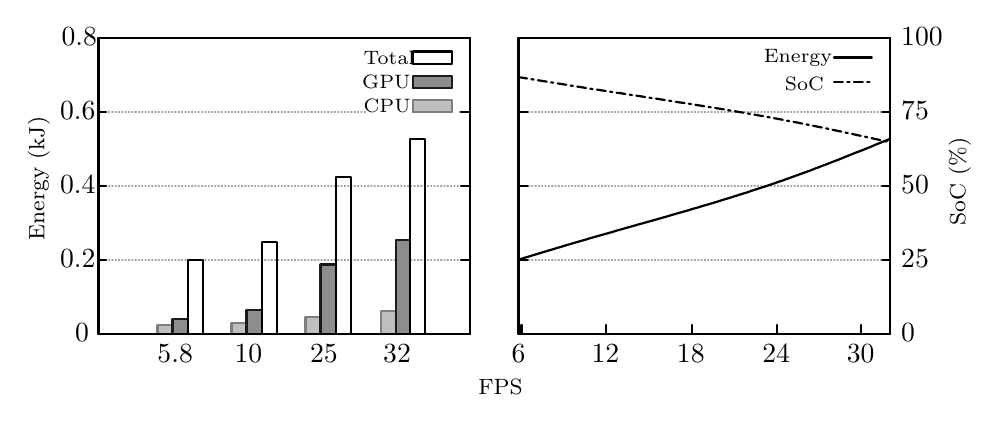
\begin{tikzpicture}[y=0.80pt, x=0.80pt, yscale=-0.680000, xscale=0.680000, inner sep=0pt, outer sep=0pt]
\begin{scope}[draw=black,line join=bevel,line cap=rect,even odd rule,line width=0.800pt]
  \begin{scope}[cm={{1.0,0.0,0.0,1.0,(0.0,0.0)}},draw=black,line join=bevel,line cap=rect,line width=0.800pt]
  \end{scope}
  \begin{scope}[cm={{1.00313,0.0,0.0,1.00313,(0.0,0.0)}},draw=black,line join=bevel,line cap=rect,line width=0.800pt]
  \end{scope}
  \begin{scope}[cm={{1.00313,0.0,0.0,1.00313,(0.0,0.0)}},draw=ca0a0a4,dash pattern=on 0.40pt off 0.80pt,line join=round,line cap=round,line width=0.400pt]
    \path[draw] (64.5000,224.5000) -- (310.5000,224.5000);
  \end{scope}
  \begin{scope}[cm={{1.00313,0.0,0.0,1.00313,(0.0,0.0)}},draw=black,line join=round,line cap=round,line width=0.800pt]
    \path[draw] (64.5000,224.5000) -- (69.5000,224.5000);
    \path[draw] (310.5000,224.5000) -- (304.5000,224.5000);
  \end{scope}
  \begin{scope}[cm={{1.00313,0.0,0.0,1.00313,(0.0,0.0)}},draw=black,line join=bevel,line cap=rect,line width=0.800pt]
  \end{scope}
  \begin{scope}[cm={{1.00313,0.0,0.0,1.00313,(49.1531,230.217)}},draw=black,line join=bevel,line cap=rect,line width=0.800pt]
  \end{scope}
  \begin{scope}[cm={{1.00313,0.0,0.0,1.00313,(49.1531,230.217)}},draw=black,line join=bevel,line cap=rect,line width=0.800pt]
  \end{scope}
  \begin{scope}[cm={{1.00313,0.0,0.0,1.00313,(49.1531,230.217)}},draw=black,line join=bevel,line cap=rect,line width=0.800pt]
  \end{scope}
  \begin{scope}[cm={{1.00313,0.0,0.0,1.00313,(49.1531,230.217)}},draw=black,line join=bevel,line cap=rect,line width=0.800pt]
  \end{scope}
  \begin{scope}[cm={{1.00313,0.0,0.0,1.00313,(49.1531,230.217)}},draw=black,line join=bevel,line cap=rect,line width=0.800pt]
  \end{scope}
  \begin{scope}[cm={{1.00313,0.0,0.0,1.00313,(49.1531,230.217)}},draw=black,line join=bevel,line cap=rect,line width=0.800pt]
    \path[fill=black] (0.0000,0.0000) node[above right] () {0};
  \end{scope}
  \begin{scope}[cm={{1.00313,0.0,0.0,1.00313,(49.1531,230.217)}},draw=black,line join=bevel,line cap=rect,line width=0.800pt]
  \end{scope}
  \begin{scope}[cm={{1.00313,0.0,0.0,1.00313,(0.0,0.0)}},draw=black,line join=bevel,line cap=rect,line width=0.800pt]
  \end{scope}
  \begin{scope}[cm={{1.00313,0.0,0.0,1.00313,(0.0,0.0)}},draw=ca0a0a4,dash pattern=on 0.40pt off 0.80pt,line join=round,line cap=round,line width=0.400pt]
    \path[draw] (64.5000,175.5000) -- (310.5000,175.5000);
  \end{scope}
  \begin{scope}[cm={{1.00313,0.0,0.0,1.00313,(0.0,0.0)}},draw=black,line join=round,line cap=round,line width=0.800pt]
    \path[draw] (64.5000,175.5000) -- (69.5000,175.5000);
    \path[draw] (310.5000,175.5000) -- (304.5000,175.5000);
  \end{scope}
  \begin{scope}[cm={{1.00313,0.0,0.0,1.00313,(0.0,0.0)}},draw=black,line join=bevel,line cap=rect,line width=0.800pt]
  \end{scope}
  \begin{scope}[cm={{1.00313,0.0,0.0,1.00313,(49.1531,181.064)}},draw=black,line join=bevel,line cap=rect,line width=0.800pt]
  \end{scope}
  \begin{scope}[cm={{1.00313,0.0,0.0,1.00313,(49.1531,181.064)}},draw=black,line join=bevel,line cap=rect,line width=0.800pt]
  \end{scope}
  \begin{scope}[cm={{1.00313,0.0,0.0,1.00313,(49.1531,181.064)}},draw=black,line join=bevel,line cap=rect,line width=0.800pt]
  \end{scope}
  \begin{scope}[cm={{1.00313,0.0,0.0,1.00313,(49.1531,181.064)}},draw=black,line join=bevel,line cap=rect,line width=0.800pt]
  \end{scope}
  \begin{scope}[cm={{1.00313,0.0,0.0,1.00313,(49.1531,181.064)}},draw=black,line join=bevel,line cap=rect,line width=0.800pt]
  \end{scope}
  \begin{scope}[cm={{1.00313,0.0,0.0,1.00313,(39.1531,181.064)}},draw=black,line join=bevel,line cap=rect,line width=0.800pt]
    \path[fill=black] (0.0000,0.0000) node[above right] () {0.2};
  \end{scope}
  \begin{scope}[cm={{1.00313,0.0,0.0,1.00313,(49.1531,181.064)}},draw=black,line join=bevel,line cap=rect,line width=0.800pt]
  \end{scope}
  \begin{scope}[cm={{1.00313,0.0,0.0,1.00313,(0.0,0.0)}},draw=black,line join=bevel,line cap=rect,line width=0.800pt]
  \end{scope}
  \begin{scope}[cm={{1.00313,0.0,0.0,1.00313,(0.0,0.0)}},draw=ca0a0a4,dash pattern=on 0.40pt off 0.80pt,line join=round,line cap=round,line width=0.400pt]
    \path[draw] (64.5000,126.5000) -- (310.5000,126.5000);
  \end{scope}
  \begin{scope}[cm={{1.00313,0.0,0.0,1.00313,(0.0,0.0)}},draw=black,line join=round,line cap=round,line width=0.800pt]
    \path[draw] (64.5000,126.5000) -- (69.5000,126.5000);
    \path[draw] (310.5000,126.5000) -- (304.5000,126.5000);
  \end{scope}
  \begin{scope}[cm={{1.00313,0.0,0.0,1.00313,(0.0,0.0)}},draw=black,line join=bevel,line cap=rect,line width=0.800pt]
  \end{scope}
  \begin{scope}[cm={{1.00313,0.0,0.0,1.00313,(49.1531,131.911)}},draw=black,line join=bevel,line cap=rect,line width=0.800pt]
  \end{scope}
  \begin{scope}[cm={{1.00313,0.0,0.0,1.00313,(49.1531,131.911)}},draw=black,line join=bevel,line cap=rect,line width=0.800pt]
  \end{scope}
  \begin{scope}[cm={{1.00313,0.0,0.0,1.00313,(49.1531,131.911)}},draw=black,line join=bevel,line cap=rect,line width=0.800pt]
  \end{scope}
  \begin{scope}[cm={{1.00313,0.0,0.0,1.00313,(49.1531,131.911)}},draw=black,line join=bevel,line cap=rect,line width=0.800pt]
  \end{scope}
  \begin{scope}[cm={{1.00313,0.0,0.0,1.00313,(49.1531,131.911)}},draw=black,line join=bevel,line cap=rect,line width=0.800pt]
  \end{scope}
  \begin{scope}[cm={{1.00313,0.0,0.0,1.00313,(39.1531,131.911)}},draw=black,line join=bevel,line cap=rect,line width=0.800pt]
    \path[fill=black] (0.0000,0.0000) node[above right] () {0.4};
  \end{scope}
  \begin{scope}[cm={{1.00313,0.0,0.0,1.00313,(49.1531,131.911)}},draw=black,line join=bevel,line cap=rect,line width=0.800pt]
  \end{scope}
  \begin{scope}[cm={{1.00313,0.0,0.0,1.00313,(0.0,0.0)}},draw=black,line join=bevel,line cap=rect,line width=0.800pt]
  \end{scope}
  \begin{scope}[cm={{1.00313,0.0,0.0,1.00313,(0.0,0.0)}},draw=ca0a0a4,dash pattern=on 0.40pt off 0.80pt,line join=round,line cap=round,line width=0.400pt]
    \path[draw] (64.5000,77.5000) -- (242.5000,77.5000);
    \path[draw] (303.5000,77.5000) -- (310.5000,77.5000);
  \end{scope}
  \begin{scope}[cm={{1.00313,0.0,0.0,1.00313,(0.0,0.0)}},draw=black,line join=round,line cap=round,line width=0.800pt]
    \path[draw] (64.5000,77.5000) -- (69.5000,77.5000);
    \path[draw] (310.5000,77.5000) -- (304.5000,77.5000);
  \end{scope}
  \begin{scope}[cm={{1.00313,0.0,0.0,1.00313,(0.0,0.0)}},draw=black,line join=bevel,line cap=rect,line width=0.800pt]
  \end{scope}
  \begin{scope}[cm={{1.00313,0.0,0.0,1.00313,(49.1531,82.7578)}},draw=black,line join=bevel,line cap=rect,line width=0.800pt]
  \end{scope}
  \begin{scope}[cm={{1.00313,0.0,0.0,1.00313,(49.1531,82.7578)}},draw=black,line join=bevel,line cap=rect,line width=0.800pt]
  \end{scope}
  \begin{scope}[cm={{1.00313,0.0,0.0,1.00313,(49.1531,82.7578)}},draw=black,line join=bevel,line cap=rect,line width=0.800pt]
  \end{scope}
  \begin{scope}[cm={{1.00313,0.0,0.0,1.00313,(49.1531,82.7578)}},draw=black,line join=bevel,line cap=rect,line width=0.800pt]
  \end{scope}
  \begin{scope}[cm={{1.00313,0.0,0.0,1.00313,(49.1531,82.7578)}},draw=black,line join=bevel,line cap=rect,line width=0.800pt]
  \end{scope}
  \begin{scope}[cm={{1.00313,0.0,0.0,1.00313,(39.1531,82.7578)}},draw=black,line join=bevel,line cap=rect,line width=0.800pt]
    \path[fill=black] (0.0000,0.0000) node[above right] () {0.6};
  \end{scope}
  \begin{scope}[cm={{1.00313,0.0,0.0,1.00313,(49.1531,82.7578)}},draw=black,line join=bevel,line cap=rect,line width=0.800pt]
  \end{scope}
  \begin{scope}[cm={{1.00313,0.0,0.0,1.00313,(0.0,0.0)}},draw=black,line join=bevel,line cap=rect,line width=0.800pt]
  \end{scope}
  \begin{scope}[cm={{1.00313,0.0,0.0,1.00313,(0.0,0.0)}},draw=ca0a0a4,dash pattern=on 0.40pt off 0.80pt,line join=round,line cap=round,line width=0.400pt]
    \path[draw] (64.5000,28.5000) -- (310.5000,28.5000);
  \end{scope}
  \begin{scope}[cm={{1.00313,0.0,0.0,1.00313,(0.0,0.0)}},draw=black,line join=round,line cap=round,line width=0.800pt]
    \path[draw] (64.5000,28.5000) -- (69.5000,28.5000);
    \path[draw] (310.5000,28.5000) -- (304.5000,28.5000);
  \end{scope}
  \begin{scope}[cm={{1.00313,0.0,0.0,1.00313,(0.0,0.0)}},draw=black,line join=bevel,line cap=rect,line width=0.800pt]
  \end{scope}
  \begin{scope}[cm={{1.00313,0.0,0.0,1.00313,(50.1562,33.6047)}},draw=black,line join=bevel,line cap=rect,line width=0.800pt]
  \end{scope}
  \begin{scope}[cm={{1.00313,0.0,0.0,1.00313,(50.1562,33.6047)}},draw=black,line join=bevel,line cap=rect,line width=0.800pt]
  \end{scope}
  \begin{scope}[cm={{1.00313,0.0,0.0,1.00313,(50.1562,33.6047)}},draw=black,line join=bevel,line cap=rect,line width=0.800pt]
  \end{scope}
  \begin{scope}[cm={{1.00313,0.0,0.0,1.00313,(50.1562,33.6047)}},draw=black,line join=bevel,line cap=rect,line width=0.800pt]
  \end{scope}
  \begin{scope}[cm={{1.00313,0.0,0.0,1.00313,(50.1562,33.6047)}},draw=black,line join=bevel,line cap=rect,line width=0.800pt]
  \end{scope}
  \begin{scope}[cm={{1.00313,0.0,0.0,1.00313,(40.1562,33.6047)}},draw=black,line join=bevel,line cap=rect,line width=0.800pt]
    \path[fill=black] (0.0000,0.0000) node[above right] () {0.8};
  \end{scope}
  \begin{scope}[cm={{1.00313,0.0,0.0,1.00313,(50.1562,33.6047)}},draw=black,line join=bevel,line cap=rect,line width=0.800pt]
  \end{scope}
  \begin{scope}[cm={{1.00313,0.0,0.0,1.00313,(0.0,0.0)}},draw=black,line join=bevel,line cap=rect,line width=0.800pt]
  \end{scope}
  \begin{scope}[cm={{1.00313,0.0,0.0,1.00313,(0.0,0.0)}},draw=black,line join=round,line cap=round,line width=0.800pt]
    \path[draw] (113.5000,224.5000) -- (113.5000,224.5000);
  \end{scope}
  \begin{scope}[cm={{1.00313,0.0,0.0,1.00313,(0.0,0.0)}},draw=black,line join=bevel,line cap=rect,line width=0.800pt]
  \end{scope}
  \begin{scope}[cm={{1.00313,0.0,0.0,1.00313,(103.823,244.261)}},draw=black,line join=bevel,line cap=rect,line width=0.800pt]
  \end{scope}
  \begin{scope}[cm={{1.00313,0.0,0.0,1.00313,(103.823,244.261)}},draw=black,line join=bevel,line cap=rect,line width=0.800pt]
  \end{scope}
  \begin{scope}[cm={{1.00313,0.0,0.0,1.00313,(103.823,244.261)}},draw=black,line join=bevel,line cap=rect,line width=0.800pt]
  \end{scope}
  \begin{scope}[cm={{1.00313,0.0,0.0,1.00313,(103.823,244.261)}},draw=black,line join=bevel,line cap=rect,line width=0.800pt]
  \end{scope}
  \begin{scope}[cm={{1.00313,0.0,0.0,1.00313,(103.823,244.261)}},draw=black,line join=bevel,line cap=rect,line width=0.800pt]
  \end{scope}
  \begin{scope}[cm={{1.00313,0.0,0.0,1.00313,(103.823,244.261)}},draw=black,line join=bevel,line cap=rect,line width=0.800pt]
    \path[fill=black] (0.0000,0.0000) node[above right] () {5.8};
  \end{scope}
  \begin{scope}[cm={{1.00313,0.0,0.0,1.00313,(103.823,244.261)}},draw=black,line join=bevel,line cap=rect,line width=0.800pt]
  \end{scope}
  \begin{scope}[cm={{1.00313,0.0,0.0,1.00313,(0.0,0.0)}},draw=black,line join=bevel,line cap=rect,line width=0.800pt]
  \end{scope}
  \begin{scope}[cm={{1.00313,0.0,0.0,1.00313,(0.0,0.0)}},draw=black,line join=round,line cap=round,line width=0.800pt]
    \path[draw] (162.5000,224.5000) -- (162.5000,224.5000);
  \end{scope}
  \begin{scope}[cm={{1.00313,0.0,0.0,1.00313,(0.0,0.0)}},draw=black,line join=bevel,line cap=rect,line width=0.800pt]
  \end{scope}
  \begin{scope}[cm={{1.00313,0.0,0.0,1.00313,(154.983,244.261)}},draw=black,line join=bevel,line cap=rect,line width=0.800pt]
  \end{scope}
  \begin{scope}[cm={{1.00313,0.0,0.0,1.00313,(154.983,244.261)}},draw=black,line join=bevel,line cap=rect,line width=0.800pt]
  \end{scope}
  \begin{scope}[cm={{1.00313,0.0,0.0,1.00313,(154.983,244.261)}},draw=black,line join=bevel,line cap=rect,line width=0.800pt]
  \end{scope}
  \begin{scope}[cm={{1.00313,0.0,0.0,1.00313,(154.983,244.261)}},draw=black,line join=bevel,line cap=rect,line width=0.800pt]
  \end{scope}
  \begin{scope}[cm={{1.00313,0.0,0.0,1.00313,(154.983,244.261)}},draw=black,line join=bevel,line cap=rect,line width=0.800pt]
  \end{scope}
  \begin{scope}[cm={{1.00313,0.0,0.0,1.00313,(154.983,244.261)}},draw=black,line join=bevel,line cap=rect,line width=0.800pt]
    \path[fill=black] (0.0000,0.0000) node[above right] () {10};
  \end{scope}
  \begin{scope}[cm={{1.00313,0.0,0.0,1.00313,(154.983,244.261)}},draw=black,line join=bevel,line cap=rect,line width=0.800pt]
  \end{scope}
  \begin{scope}[cm={{1.00313,0.0,0.0,1.00313,(0.0,0.0)}},draw=black,line join=bevel,line cap=rect,line width=0.800pt]
  \end{scope}
  \begin{scope}[cm={{1.00313,0.0,0.0,1.00313,(0.0,0.0)}},draw=black,line join=round,line cap=round,line width=0.800pt]
    \path[draw] (211.5000,224.5000) -- (211.5000,224.5000);
  \end{scope}
  \begin{scope}[cm={{1.00313,0.0,0.0,1.00313,(0.0,0.0)}},draw=black,line join=bevel,line cap=rect,line width=0.800pt]
  \end{scope}
  \begin{scope}[cm={{1.00313,0.0,0.0,1.00313,(205.139,244.261)}},draw=black,line join=bevel,line cap=rect,line width=0.800pt]
  \end{scope}
  \begin{scope}[cm={{1.00313,0.0,0.0,1.00313,(205.139,244.261)}},draw=black,line join=bevel,line cap=rect,line width=0.800pt]
  \end{scope}
  \begin{scope}[cm={{1.00313,0.0,0.0,1.00313,(205.139,244.261)}},draw=black,line join=bevel,line cap=rect,line width=0.800pt]
  \end{scope}
  \begin{scope}[cm={{1.00313,0.0,0.0,1.00313,(205.139,244.261)}},draw=black,line join=bevel,line cap=rect,line width=0.800pt]
  \end{scope}
  \begin{scope}[cm={{1.00313,0.0,0.0,1.00313,(205.139,244.261)}},draw=black,line join=bevel,line cap=rect,line width=0.800pt]
  \end{scope}
  \begin{scope}[cm={{1.00313,0.0,0.0,1.00313,(205.139,244.261)}},draw=black,line join=bevel,line cap=rect,line width=0.800pt]
    \path[fill=black] (0.0000,0.0000) node[above right] () {25};
  \end{scope}
  \begin{scope}[cm={{1.00313,0.0,0.0,1.00313,(205.139,244.261)}},draw=black,line join=bevel,line cap=rect,line width=0.800pt]
  \end{scope}
  \begin{scope}[cm={{1.00313,0.0,0.0,1.00313,(0.0,0.0)}},draw=black,line join=bevel,line cap=rect,line width=0.800pt]
  \end{scope}
  \begin{scope}[cm={{1.00313,0.0,0.0,1.00313,(0.0,0.0)}},draw=black,line join=round,line cap=round,line width=0.800pt]
    \path[draw] (261.5000,224.5000) -- (261.5000,224.5000);
  \end{scope}
  \begin{scope}[cm={{1.00313,0.0,0.0,1.00313,(0.0,0.0)}},draw=black,line join=bevel,line cap=rect,line width=0.800pt]
  \end{scope}
  \begin{scope}[cm={{1.00313,0.0,0.0,1.00313,(253.791,244.261)}},draw=black,line join=bevel,line cap=rect,line width=0.800pt]
  \end{scope}
  \begin{scope}[cm={{1.00313,0.0,0.0,1.00313,(253.791,244.261)}},draw=black,line join=bevel,line cap=rect,line width=0.800pt]
  \end{scope}
  \begin{scope}[cm={{1.00313,0.0,0.0,1.00313,(253.791,244.261)}},draw=black,line join=bevel,line cap=rect,line width=0.800pt]
  \end{scope}
  \begin{scope}[cm={{1.00313,0.0,0.0,1.00313,(253.791,244.261)}},draw=black,line join=bevel,line cap=rect,line width=0.800pt]
  \end{scope}
  \begin{scope}[cm={{1.00313,0.0,0.0,1.00313,(253.791,244.261)}},draw=black,line join=bevel,line cap=rect,line width=0.800pt]
  \end{scope}
  \begin{scope}[cm={{1.00313,0.0,0.0,1.00313,(253.791,244.261)}},draw=black,line join=bevel,line cap=rect,line width=0.800pt]
    \path[fill=black] (0.0000,0.0000) node[above right] () {32};
  \end{scope}
  \begin{scope}[cm={{1.00313,0.0,0.0,1.00313,(253.791,244.261)}},draw=black,line join=bevel,line cap=rect,line width=0.800pt]
  \end{scope}
  \begin{scope}[cm={{1.00313,0.0,0.0,1.00313,(0.0,0.0)}},draw=black,line join=bevel,line cap=rect,line width=0.800pt]
  \end{scope}
  \begin{scope}[cm={{1.00313,0.0,0.0,1.00313,(0.0,0.0)}},draw=black,line join=round,line cap=round,line width=0.800pt]
    \path[draw] (64.5000,28.5000) -- (64.5000,224.5000) -- (310.5000,224.5000) --
      (310.5000,28.5000) -- (64.5000,28.5000);
  \end{scope}
  \begin{scope}[cm={{1.00313,0.0,0.0,1.00313,(0.0,0.0)}},draw=black,line join=bevel,line cap=rect,line width=0.800pt]
  \end{scope}
  \begin{scope}[cm={{0.0,-1.00313,1.00313,0.0,(31.5984,163.008)}},draw=black,line join=bevel,line cap=rect,line width=0.800pt]
  \end{scope}
  \begin{scope}[cm={{0.0,-1.00313,1.00313,0.0,(31.5984,163.008)}},draw=black,line join=bevel,line cap=rect,line width=0.800pt]
  \end{scope}
  \begin{scope}[cm={{0.0,-1.00313,1.00313,0.0,(31.5984,163.008)}},draw=black,line join=bevel,line cap=rect,line width=0.800pt]
  \end{scope}
  \begin{scope}[cm={{0.0,-1.00313,1.00313,0.0,(31.5984,163.008)}},draw=black,line join=bevel,line cap=rect,line width=0.800pt]
  \end{scope}
  \begin{scope}[cm={{0.0,-1.00313,1.00313,0.0,(31.5984,163.008)}},draw=black,line join=bevel,line cap=rect,line width=0.800pt]
  \end{scope}
  \begin{scope}[cm={{0.0,-1.00313,1.00313,0.0,(17.5984,163.008)}},draw=black,line join=bevel,line cap=rect,line width=0.800pt]
    \path[fill=black] (0.0000,0.0000) node[above right] () {\rotatebox{90}{\footnotesize Energy (kJ)}};
  \end{scope}
  \begin{scope}[cm={{0.0,-1.00313,1.00313,0.0,(31.5984,163.008)}},draw=black,line join=bevel,line cap=rect,line width=0.800pt]
  \end{scope}
  \begin{scope}[cm={{1.00313,0.0,0.0,1.00313,(316.988,265.327)}},draw=black,line join=bevel,line cap=rect,line width=0.800pt]
  \end{scope}
  \begin{scope}[cm={{1.00313,0.0,0.0,1.00313,(316.988,265.327)}},draw=black,line join=bevel,line cap=rect,line width=0.800pt]
  \end{scope}
  \begin{scope}[cm={{1.00313,0.0,0.0,1.00313,(316.988,265.327)}},draw=black,line join=bevel,line cap=rect,line width=0.800pt]
  \end{scope}
  \begin{scope}[cm={{1.00313,0.0,0.0,1.00313,(316.988,265.327)}},draw=black,line join=bevel,line cap=rect,line width=0.800pt]
  \end{scope}
  \begin{scope}[cm={{1.00313,0.0,0.0,1.00313,(316.988,265.327)}},draw=black,line join=bevel,line cap=rect,line width=0.800pt]
  \end{scope}
  \begin{scope}[cm={{1.00313,0.0,0.0,1.00313,(316.988,265.327)}},draw=black,line join=bevel,line cap=rect,line width=0.800pt]
    \path[fill=black] (0.0000,0.0000) node[above right] () {\footnotesize FPS};
  \end{scope}
  \begin{scope}[cm={{1.00313,0.0,0.0,1.00313,(316.988,265.327)}},draw=black,line join=bevel,line cap=rect,line width=0.800pt]
  \end{scope}
  \begin{scope}[cm={{1.00313,0.0,0.0,1.00313,(247.772,78.2438)}},draw=black,line join=bevel,line cap=rect,line width=0.800pt]
  \end{scope}
  \begin{scope}[cm={{1.00313,0.0,0.0,1.00313,(247.772,78.2438)}},draw=black,line join=bevel,line cap=rect,line width=0.800pt]
  \end{scope}
  \begin{scope}[cm={{1.00313,0.0,0.0,1.00313,(247.772,78.2438)}},draw=black,line join=bevel,line cap=rect,line width=0.800pt]
  \end{scope}
  \begin{scope}[cm={{1.00313,0.0,0.0,1.00313,(247.772,78.2438)}},draw=black,line join=bevel,line cap=rect,line width=0.800pt]
  \end{scope}
  \begin{scope}[cm={{1.00313,0.0,0.0,1.00313,(247.772,78.2438)}},draw=black,line join=bevel,line cap=rect,line width=0.800pt]
  \end{scope}
  \begin{scope}[cm={{1.00313,0.0,0.0,1.00313,(240.772,78.2438)}},draw=black,line join=bevel,line cap=rect,line width=0.800pt]
    \path[fill=black] (0.0000,0.0000) node[above right] () {\scriptsize CPU};
  \end{scope}
  \begin{scope}[cm={{1.00313,0.0,0.0,1.00313,(247.772,78.2438)}},draw=black,line join=bevel,line cap=rect,line width=0.800pt]
  \end{scope}
  \begin{scope}[cm={{1.00313,0.0,0.0,1.00313,(0.0,0.0)}},draw=black,line join=bevel,line cap=rect,line width=0.800pt]
  \end{scope}
  \begin{scope}[cm={{1.00313,0.0,0.0,1.00313,(0.0,0.0)}},fill=cbfbfbf]
    \path[fill,rounded corners=0.0000cm] (273.0000,70.0000) rectangle
      (299.0000,78.0000);
  \end{scope}
  \begin{scope}[cm={{1.00313,0.0,0.0,1.00313,(0.0,0.0)}},draw=black,line join=bevel,line cap=rect,line width=0.800pt]
  \end{scope}
  \begin{scope}[cm={{1.00313,0.0,0.0,1.00313,(0.0,0.0)}},draw=black,line join=bevel,line cap=rect,line width=0.800pt]
  \end{scope}
  \begin{scope}[cm={{1.00313,0.0,0.0,1.00313,(0.0,0.0)}},draw=c7f7f7f,line join=round,line cap=round,line width=0.800pt]
    \path[draw,even odd rule] (272.5000,77.5000) -- (298.5000,77.5000) --
      (298.5000,77.5000) -- (298.5000,69.5000) -- (298.5000,69.5000) --
      (272.5000,69.5000) -- (272.5000,69.5000) -- (272.5000,77.5000);
  \end{scope}
  \begin{scope}[cm={{1.00313,0.0,0.0,1.00313,(0.0,0.0)}},draw=black,line join=bevel,line cap=rect,line width=0.800pt]
  \end{scope}
  \begin{scope}[cm={{1.00313,0.0,0.0,1.00313,(0.0,0.0)}},draw=black,line join=bevel,line cap=rect,line width=0.800pt]
  \end{scope}
  \begin{scope}[cm={{1.00313,0.0,0.0,1.00313,(0.0,0.0)}},draw=black,line join=bevel,line cap=rect,line width=0.800pt]
  \end{scope}
  \begin{scope}[cm={{1.00313,0.0,0.0,1.00313,(0.0,0.0)}},draw=black,line join=bevel,line cap=rect,line width=0.800pt]
  \end{scope}
  \begin{scope}[cm={{1.00313,0.0,0.0,1.00313,(0.0,0.0)}},fill=cbfbfbf]
    \path[fill,rounded corners=0.0000cm] (103.0000,219.0000) rectangle
      (113.0000,224.0000);
  \end{scope}
  \begin{scope}[cm={{1.00313,0.0,0.0,1.00313,(0.0,0.0)}},draw=black,line join=bevel,line cap=rect,line width=0.800pt]
  \end{scope}
  \begin{scope}[cm={{1.00313,0.0,0.0,1.00313,(0.0,0.0)}},draw=black,line join=bevel,line cap=rect,line width=0.800pt]
  \end{scope}
  \begin{scope}[cm={{1.00313,0.0,0.0,1.00313,(0.0,0.0)}},draw=c7f7f7f,line join=round,line cap=round,line width=0.800pt]
    \path[draw] (103.5000,224.5000) -- (103.5000,218.5000) -- (113.5000,218.5000) --
      (113.5000,224.5000) -- (103.5000,224.5000);
  \end{scope}
  \begin{scope}[cm={{1.00313,0.0,0.0,1.00313,(0.0,0.0)}},draw=black,line join=bevel,line cap=rect,line width=0.800pt]
  \end{scope}
  \begin{scope}[cm={{1.00313,0.0,0.0,1.00313,(0.0,0.0)}},draw=black,line join=bevel,line cap=rect,line width=0.800pt]
  \end{scope}
  \begin{scope}[cm={{1.00313,0.0,0.0,1.00313,(0.0,0.0)}},fill=cbfbfbf]
    \path[fill,rounded corners=0.0000cm] (153.0000,218.0000) rectangle
      (163.0000,224.0000);
  \end{scope}
  \begin{scope}[cm={{1.00313,0.0,0.0,1.00313,(0.0,0.0)}},draw=black,line join=bevel,line cap=rect,line width=0.800pt]
  \end{scope}
  \begin{scope}[cm={{1.00313,0.0,0.0,1.00313,(0.0,0.0)}},draw=black,line join=bevel,line cap=rect,line width=0.800pt]
  \end{scope}
  \begin{scope}[cm={{1.00313,0.0,0.0,1.00313,(0.0,0.0)}},draw=c7f7f7f,line join=round,line cap=round,line width=0.800pt]
    \path[draw] (152.5000,224.5000) -- (152.5000,217.5000) -- (162.5000,217.5000) --
      (162.5000,224.5000) -- (152.5000,224.5000);
  \end{scope}
  \begin{scope}[cm={{1.00313,0.0,0.0,1.00313,(0.0,0.0)}},draw=black,line join=bevel,line cap=rect,line width=0.800pt]
  \end{scope}
  \begin{scope}[cm={{1.00313,0.0,0.0,1.00313,(0.0,0.0)}},draw=black,line join=bevel,line cap=rect,line width=0.800pt]
  \end{scope}
  \begin{scope}[cm={{1.00313,0.0,0.0,1.00313,(0.0,0.0)}},fill=cbfbfbf]
    \path[fill,rounded corners=0.0000cm] (202.0000,213.0000) rectangle
      (212.0000,224.0000);
  \end{scope}
  \begin{scope}[cm={{1.00313,0.0,0.0,1.00313,(0.0,0.0)}},draw=black,line join=bevel,line cap=rect,line width=0.800pt]
  \end{scope}
  \begin{scope}[cm={{1.00313,0.0,0.0,1.00313,(0.0,0.0)}},draw=black,line join=bevel,line cap=rect,line width=0.800pt]
  \end{scope}
  \begin{scope}[cm={{1.00313,0.0,0.0,1.00313,(0.0,0.0)}},draw=c7f7f7f,line join=round,line cap=round,line width=0.800pt]
    \path[draw] (201.5000,224.5000) -- (201.5000,213.5000) -- (211.5000,213.5000) --
      (211.5000,224.5000) -- (201.5000,224.5000);
  \end{scope}
  \begin{scope}[cm={{1.00313,0.0,0.0,1.00313,(0.0,0.0)}},draw=black,line join=bevel,line cap=rect,line width=0.800pt]
  \end{scope}
  \begin{scope}[cm={{1.00313,0.0,0.0,1.00313,(0.0,0.0)}},draw=black,line join=bevel,line cap=rect,line width=0.800pt]
  \end{scope}
  \begin{scope}[cm={{1.00313,0.0,0.0,1.00313,(0.0,0.0)}},fill=cbfbfbf]
    \path[fill,rounded corners=0.0000cm] (251.0000,209.0000) rectangle
      (261.0000,224.0000);
  \end{scope}
  \begin{scope}[cm={{1.00313,0.0,0.0,1.00313,(0.0,0.0)}},draw=black,line join=bevel,line cap=rect,line width=0.800pt]
  \end{scope}
  \begin{scope}[cm={{1.00313,0.0,0.0,1.00313,(0.0,0.0)}},draw=black,line join=bevel,line cap=rect,line width=0.800pt]
  \end{scope}
  \begin{scope}[cm={{1.00313,0.0,0.0,1.00313,(0.0,0.0)}},draw=c7f7f7f,line join=round,line cap=round,line width=0.800pt]
    \path[draw] (251.5000,224.5000) -- (251.5000,209.5000) -- (261.5000,209.5000) --
      (261.5000,224.5000) -- (251.5000,224.5000);
  \end{scope}
  \begin{scope}[cm={{1.00313,0.0,0.0,1.00313,(0.0,0.0)}},draw=black,line join=bevel,line cap=rect,line width=0.800pt]
  \end{scope}
  \begin{scope}[cm={{1.00313,0.0,0.0,1.00313,(246.769,62.1938)}},draw=black,line join=bevel,line cap=rect,line width=0.800pt]
  \end{scope}
  \begin{scope}[cm={{1.00313,0.0,0.0,1.00313,(246.769,62.1938)}},draw=black,line join=bevel,line cap=rect,line width=0.800pt]
  \end{scope}
  \begin{scope}[cm={{1.00313,0.0,0.0,1.00313,(246.769,62.1938)}},draw=black,line join=bevel,line cap=rect,line width=0.800pt]
  \end{scope}
  \begin{scope}[cm={{1.00313,0.0,0.0,1.00313,(246.769,62.1938)}},draw=black,line join=bevel,line cap=rect,line width=0.800pt]
  \end{scope}
  \begin{scope}[cm={{1.00313,0.0,0.0,1.00313,(246.769,62.1938)}},draw=black,line join=bevel,line cap=rect,line width=0.800pt]
  \end{scope}
  \begin{scope}[cm={{1.00313,0.0,0.0,1.00313,(239.769,62.1938)}},draw=black,line join=bevel,line cap=rect,line width=0.800pt]
    \path[fill=black] (0.0000,0.0000) node[above right] () {\scriptsize GPU};
  \end{scope}
  \begin{scope}[cm={{1.00313,0.0,0.0,1.00313,(246.769,62.1938)}},draw=black,line join=bevel,line cap=rect,line width=0.800pt]
  \end{scope}
  \begin{scope}[cm={{1.00313,0.0,0.0,1.00313,(0.0,0.0)}},draw=black,line join=bevel,line cap=rect,line width=0.800pt]
  \end{scope}
  \begin{scope}[cm={{1.00313,0.0,0.0,1.00313,(0.0,0.0)}},fill=c8d8d8d]
    \path[fill,rounded corners=0.0000cm] (273.0000,54.0000) rectangle
      (299.0000,62.0000);
  \end{scope}
  \begin{scope}[cm={{1.00313,0.0,0.0,1.00313,(0.0,0.0)}},draw=black,line join=bevel,line cap=rect,line width=0.800pt]
  \end{scope}
  \begin{scope}[cm={{1.00313,0.0,0.0,1.00313,(0.0,0.0)}},draw=black,line join=bevel,line cap=rect,line width=0.800pt]
  \end{scope}
  \begin{scope}[cm={{1.00313,0.0,0.0,1.00313,(0.0,0.0)}},draw=c1a1a1a,line join=round,line cap=round,line width=0.800pt]
    \path[draw,even odd rule] (272.5000,61.5000) -- (298.5000,61.5000) --
      (298.5000,61.5000) -- (298.5000,53.5000) -- (298.5000,53.5000) --
      (272.5000,53.5000) -- (272.5000,53.5000) -- (272.5000,61.5000);
  \end{scope}
  \begin{scope}[cm={{1.00313,0.0,0.0,1.00313,(0.0,0.0)}},draw=black,line join=bevel,line cap=rect,line width=0.800pt]
  \end{scope}
  \begin{scope}[cm={{1.00313,0.0,0.0,1.00313,(0.0,0.0)}},draw=black,line join=bevel,line cap=rect,line width=0.800pt]
  \end{scope}
  \begin{scope}[cm={{1.00313,0.0,0.0,1.00313,(0.0,0.0)}},draw=black,line join=bevel,line cap=rect,line width=0.800pt]
  \end{scope}
  \begin{scope}[cm={{1.00313,0.0,0.0,1.00313,(0.0,0.0)}},draw=black,line join=bevel,line cap=rect,line width=0.800pt]
  \end{scope}
  \begin{scope}[cm={{1.00313,0.0,0.0,1.00313,(0.0,0.0)}},fill=c8d8d8d]
    \path[fill,rounded corners=0.0000cm] (113.0000,214.0000) rectangle
      (123.0000,224.0000);
  \end{scope}
  \begin{scope}[cm={{1.00313,0.0,0.0,1.00313,(0.0,0.0)}},draw=black,line join=bevel,line cap=rect,line width=0.800pt]
  \end{scope}
  \begin{scope}[cm={{1.00313,0.0,0.0,1.00313,(0.0,0.0)}},draw=black,line join=bevel,line cap=rect,line width=0.800pt]
  \end{scope}
  \begin{scope}[cm={{1.00313,0.0,0.0,1.00313,(0.0,0.0)}},draw=c1a1a1a,line join=round,line cap=round,line width=0.800pt]
    \path[draw] (113.5000,224.5000) -- (113.5000,214.5000) -- (123.5000,214.5000) --
      (123.5000,224.5000) -- (113.5000,224.5000);
  \end{scope}
  \begin{scope}[cm={{1.00313,0.0,0.0,1.00313,(0.0,0.0)}},draw=black,line join=bevel,line cap=rect,line width=0.800pt]
  \end{scope}
  \begin{scope}[cm={{1.00313,0.0,0.0,1.00313,(0.0,0.0)}},draw=black,line join=bevel,line cap=rect,line width=0.800pt]
  \end{scope}
  \begin{scope}[cm={{1.00313,0.0,0.0,1.00313,(0.0,0.0)}},fill=c8d8d8d]
    \path[fill,rounded corners=0.0000cm] (163.0000,208.0000) rectangle
      (173.0000,224.0000);
  \end{scope}
  \begin{scope}[cm={{1.00313,0.0,0.0,1.00313,(0.0,0.0)}},draw=black,line join=bevel,line cap=rect,line width=0.800pt]
  \end{scope}
  \begin{scope}[cm={{1.00313,0.0,0.0,1.00313,(0.0,0.0)}},draw=black,line join=bevel,line cap=rect,line width=0.800pt]
  \end{scope}
  \begin{scope}[cm={{1.00313,0.0,0.0,1.00313,(0.0,0.0)}},draw=c1a1a1a,line join=round,line cap=round,line width=0.800pt]
    \path[draw] (162.5000,224.5000) -- (162.5000,208.5000) -- (172.5000,208.5000) --
      (172.5000,224.5000) -- (162.5000,224.5000);
  \end{scope}
  \begin{scope}[cm={{1.00313,0.0,0.0,1.00313,(0.0,0.0)}},draw=black,line join=bevel,line cap=rect,line width=0.800pt]
  \end{scope}
  \begin{scope}[cm={{1.00313,0.0,0.0,1.00313,(0.0,0.0)}},draw=black,line join=bevel,line cap=rect,line width=0.800pt]
  \end{scope}
  \begin{scope}[cm={{1.00313,0.0,0.0,1.00313,(0.0,0.0)}},fill=c8d8d8d]
    \path[fill,rounded corners=0.0000cm] (212.0000,179.0000) rectangle
      (222.0000,224.0000);
  \end{scope}
  \begin{scope}[cm={{1.00313,0.0,0.0,1.00313,(0.0,0.0)}},draw=black,line join=bevel,line cap=rect,line width=0.800pt]
  \end{scope}
  \begin{scope}[cm={{1.00313,0.0,0.0,1.00313,(0.0,0.0)}},draw=black,line join=bevel,line cap=rect,line width=0.800pt]
  \end{scope}
  \begin{scope}[cm={{1.00313,0.0,0.0,1.00313,(0.0,0.0)}},draw=c1a1a1a,line join=round,line cap=round,line width=0.800pt]
    \path[draw] (211.5000,224.5000) -- (211.5000,178.5000) -- (221.5000,178.5000) --
      (221.5000,224.5000) -- (211.5000,224.5000);
  \end{scope}
  \begin{scope}[cm={{1.00313,0.0,0.0,1.00313,(0.0,0.0)}},draw=black,line join=bevel,line cap=rect,line width=0.800pt]
  \end{scope}
  \begin{scope}[cm={{1.00313,0.0,0.0,1.00313,(0.0,0.0)}},draw=black,line join=bevel,line cap=rect,line width=0.800pt]
  \end{scope}
  \begin{scope}[cm={{1.00313,0.0,0.0,1.00313,(0.0,0.0)}},fill=c8d8d8d]
    \path[fill,rounded corners=0.0000cm] (261.0000,163.0000) rectangle
      (271.0000,224.0000);
  \end{scope}
  \begin{scope}[cm={{1.00313,0.0,0.0,1.00313,(0.0,0.0)}},draw=black,line join=bevel,line cap=rect,line width=0.800pt]
  \end{scope}
  \begin{scope}[cm={{1.00313,0.0,0.0,1.00313,(0.0,0.0)}},draw=black,line join=bevel,line cap=rect,line width=0.800pt]
  \end{scope}
  \begin{scope}[cm={{1.00313,0.0,0.0,1.00313,(0.0,0.0)}},draw=c1a1a1a,line join=round,line cap=round,line width=0.800pt]
    \path[draw] (261.5000,224.5000) -- (261.5000,162.5000) -- (270.5000,162.5000) --
      (270.5000,224.5000) -- (261.5000,224.5000);
  \end{scope}
  \begin{scope}[cm={{1.00313,0.0,0.0,1.00313,(0.0,0.0)}},draw=black,line join=bevel,line cap=rect,line width=0.800pt]
  \end{scope}
  \begin{scope}[cm={{1.00313,0.0,0.0,1.00313,(244.763,46.1438)}},draw=black,line join=bevel,line cap=rect,line width=0.800pt]
  \end{scope}
  \begin{scope}[cm={{1.00313,0.0,0.0,1.00313,(244.763,46.1438)}},draw=black,line join=bevel,line cap=rect,line width=0.800pt]
  \end{scope}
  \begin{scope}[cm={{1.00313,0.0,0.0,1.00313,(244.763,46.1438)}},draw=black,line join=bevel,line cap=rect,line width=0.800pt]
  \end{scope}
  \begin{scope}[cm={{1.00313,0.0,0.0,1.00313,(244.763,46.1438)}},draw=black,line join=bevel,line cap=rect,line width=0.800pt]
  \end{scope}
  \begin{scope}[cm={{1.00313,0.0,0.0,1.00313,(244.763,46.1438)}},draw=black,line join=bevel,line cap=rect,line width=0.800pt]
  \end{scope}
  \begin{scope}[cm={{1.00313,0.0,0.0,1.00313,(240.763,46.1438)}},draw=black,line join=bevel,line cap=rect,line width=0.800pt]
    \path[fill=black] (0.0000,0.0000) node[above right] () {\scriptsize Total};
  \end{scope}
  \begin{scope}[cm={{1.00313,0.0,0.0,1.00313,(244.763,46.1438)}},draw=black,line join=bevel,line cap=rect,line width=0.800pt]
  \end{scope}
  \begin{scope}[cm={{1.00313,0.0,0.0,1.00313,(0.0,0.0)}},draw=black,line join=bevel,line cap=rect,line width=0.800pt]
  \end{scope}
  \begin{scope}[cm={{1.00313,0.0,0.0,1.00313,(0.0,0.0)}}]
    \path[rounded corners=0.0000cm] (273.0000,38.0000) rectangle (299.0000,46.0000);
  \end{scope}
  \begin{scope}[cm={{1.00313,0.0,0.0,1.00313,(0.0,0.0)}},draw=black,line join=bevel,line cap=rect,line width=0.800pt]
  \end{scope}
  \begin{scope}[cm={{1.00313,0.0,0.0,1.00313,(0.0,0.0)}},draw=black,line join=bevel,line cap=rect,line width=0.800pt]
  \end{scope}
  \begin{scope}[cm={{1.00313,0.0,0.0,1.00313,(0.0,0.0)}},draw=black,line join=round,line cap=round,line width=0.800pt]
    \path[draw,even odd rule] (272.5000,45.5000) -- (298.5000,45.5000) --
      (298.5000,45.5000) -- (298.5000,37.5000) -- (298.5000,37.5000) --
      (272.5000,37.5000) -- (272.5000,37.5000) -- (272.5000,45.5000);
  \end{scope}
  \begin{scope}[cm={{1.00313,0.0,0.0,1.00313,(0.0,0.0)}},draw=black,line join=bevel,line cap=rect,line width=0.800pt]
  \end{scope}
  \begin{scope}[cm={{1.00313,0.0,0.0,1.00313,(0.0,0.0)}},draw=black,line join=bevel,line cap=rect,line width=0.800pt]
  \end{scope}
  \begin{scope}[cm={{1.00313,0.0,0.0,1.00313,(0.0,0.0)}},draw=black,line join=bevel,line cap=rect,line width=0.800pt]
  \end{scope}
  \begin{scope}[cm={{1.00313,0.0,0.0,1.00313,(0.0,0.0)}},draw=black,line join=bevel,line cap=rect,line width=0.800pt]
  \end{scope}
  \begin{scope}[cm={{1.00313,0.0,0.0,1.00313,(0.0,0.0)}}]
    \path[rounded corners=0.0000cm] (123.0000,175.0000) rectangle
      (133.0000,224.0000);
  \end{scope}
  \begin{scope}[cm={{1.00313,0.0,0.0,1.00313,(0.0,0.0)}},draw=black,line join=bevel,line cap=rect,line width=0.800pt]
  \end{scope}
  \begin{scope}[cm={{1.00313,0.0,0.0,1.00313,(0.0,0.0)}},draw=black,line join=bevel,line cap=rect,line width=0.800pt]
  \end{scope}
  \begin{scope}[cm={{1.00313,0.0,0.0,1.00313,(0.0,0.0)}},draw=black,line join=round,line cap=round,line width=0.800pt]
    \path[draw] (123.5000,224.5000) -- (123.5000,175.5000) -- (133.5000,175.5000) --
      (133.5000,224.5000) -- (123.5000,224.5000);
  \end{scope}
  \begin{scope}[cm={{1.00313,0.0,0.0,1.00313,(0.0,0.0)}},draw=black,line join=bevel,line cap=rect,line width=0.800pt]
  \end{scope}
  \begin{scope}[cm={{1.00313,0.0,0.0,1.00313,(0.0,0.0)}},draw=black,line join=bevel,line cap=rect,line width=0.800pt]
  \end{scope}
  \begin{scope}[cm={{1.00313,0.0,0.0,1.00313,(0.0,0.0)}}]
    \path[rounded corners=0.0000cm] (172.0000,163.0000) rectangle
      (182.0000,224.0000);
  \end{scope}
  \begin{scope}[cm={{1.00313,0.0,0.0,1.00313,(0.0,0.0)}},draw=black,line join=bevel,line cap=rect,line width=0.800pt]
  \end{scope}
  \begin{scope}[cm={{1.00313,0.0,0.0,1.00313,(0.0,0.0)}},draw=black,line join=bevel,line cap=rect,line width=0.800pt]
  \end{scope}
  \begin{scope}[cm={{1.00313,0.0,0.0,1.00313,(0.0,0.0)}},draw=black,line join=round,line cap=round,line width=0.800pt]
    \path[draw] (172.5000,224.5000) -- (172.5000,163.5000) -- (182.5000,163.5000) --
      (182.5000,224.5000) -- (172.5000,224.5000);
  \end{scope}
  \begin{scope}[cm={{1.00313,0.0,0.0,1.00313,(0.0,0.0)}},draw=black,line join=bevel,line cap=rect,line width=0.800pt]
  \end{scope}
  \begin{scope}[cm={{1.00313,0.0,0.0,1.00313,(0.0,0.0)}},draw=black,line join=bevel,line cap=rect,line width=0.800pt]
  \end{scope}
  \begin{scope}[cm={{1.00313,0.0,0.0,1.00313,(0.0,0.0)}}]
    \path[rounded corners=0.0000cm] (222.0000,121.0000) rectangle
      (232.0000,224.0000);
  \end{scope}
  \begin{scope}[cm={{1.00313,0.0,0.0,1.00313,(0.0,0.0)}},draw=black,line join=bevel,line cap=rect,line width=0.800pt]
  \end{scope}
  \begin{scope}[cm={{1.00313,0.0,0.0,1.00313,(0.0,0.0)}},draw=black,line join=bevel,line cap=rect,line width=0.800pt]
  \end{scope}
  \begin{scope}[cm={{1.00313,0.0,0.0,1.00313,(0.0,0.0)}},draw=black,line join=round,line cap=round,line width=0.800pt]
    \path[draw] (221.5000,224.5000) -- (221.5000,120.5000) -- (231.5000,120.5000) --
      (231.5000,224.5000) -- (221.5000,224.5000);
  \end{scope}
  \begin{scope}[cm={{1.00313,0.0,0.0,1.00313,(0.0,0.0)}},draw=black,line join=bevel,line cap=rect,line width=0.800pt]
  \end{scope}
  \begin{scope}[cm={{1.00313,0.0,0.0,1.00313,(0.0,0.0)}},draw=black,line join=bevel,line cap=rect,line width=0.800pt]
  \end{scope}
  \begin{scope}[cm={{1.00313,0.0,0.0,1.00313,(0.0,0.0)}}]
    \path[rounded corners=0.0000cm] (271.0000,95.0000) rectangle
      (281.0000,224.0000);
  \end{scope}
  \begin{scope}[cm={{1.00313,0.0,0.0,1.00313,(0.0,0.0)}},draw=black,line join=bevel,line cap=rect,line width=0.800pt]
  \end{scope}
  \begin{scope}[cm={{1.00313,0.0,0.0,1.00313,(0.0,0.0)}},draw=black,line join=bevel,line cap=rect,line width=0.800pt]
  \end{scope}
  \begin{scope}[cm={{1.00313,0.0,0.0,1.00313,(0.0,0.0)}},draw=black,line join=round,line cap=round,line width=0.800pt]
    \path[draw] (270.5000,224.5000) -- (270.5000,95.5000) -- (280.5000,95.5000) --
      (280.5000,224.5000) -- (270.5000,224.5000);
  \end{scope}
  \begin{scope}[cm={{1.00313,0.0,0.0,1.00313,(0.0,0.0)}},draw=black,line join=bevel,line cap=rect,line width=0.800pt]
  \end{scope}
  \begin{scope}[cm={{1.00313,0.0,0.0,1.00313,(0.0,0.0)}},draw=black,line join=bevel,line cap=rect,line width=0.800pt]
  \end{scope}
  \begin{scope}[cm={{1.00313,0.0,0.0,1.00313,(0.0,0.0)}},draw=black,line join=round,line cap=round,line width=0.800pt]
    \path[draw] (64.5000,28.5000) -- (64.5000,224.5000) -- (310.5000,224.5000) --
      (310.5000,28.5000) -- (64.5000,28.5000);
  \end{scope}
  \begin{scope}[cm={{1.00313,0.0,0.0,1.00313,(0.0,0.0)}},draw=ca0a0a4,dash pattern=on 0.40pt off 0.80pt,line join=round,line cap=round,line width=0.400pt]
    \path[draw] (342.5000,224.5000) -- (588.5000,224.5000);
  \end{scope}
  \begin{scope}[cm={{1.00313,0.0,0.0,1.00313,(0.0,0.0)}},draw=black,line join=round,line cap=round,line width=0.800pt]
    \path[draw] (342.5000,224.5000) -- (348.5000,224.5000);
    \path[draw] (588.5000,224.5000) -- (583.5000,224.5000);
  \end{scope}
  \begin{scope}[cm={{1.00313,0.0,0.0,1.00313,(0.0,0.0)}},draw=black,line join=bevel,line cap=rect,line width=0.800pt]
  \end{scope}
  \begin{scope}[cm={{1.00313,0.0,0.0,1.00313,(336.047,224.7)}},draw=black,line join=bevel,line cap=rect,line width=0.800pt]
  \end{scope}
  \begin{scope}[cm={{1.00313,0.0,0.0,1.00313,(336.047,224.7)}},draw=black,line join=bevel,line cap=rect,line width=0.800pt]
  \end{scope}
  \begin{scope}[cm={{1.00313,0.0,0.0,1.00313,(336.047,224.7)}},draw=black,line join=bevel,line cap=rect,line width=0.800pt]
  \end{scope}
  \begin{scope}[cm={{1.00313,0.0,0.0,1.00313,(336.047,224.7)}},draw=black,line join=bevel,line cap=rect,line width=0.800pt]
  \end{scope}
  \begin{scope}[cm={{1.00313,0.0,0.0,1.00313,(336.047,224.7)}},draw=black,line join=bevel,line cap=rect,line width=0.800pt]
  \end{scope}
  \begin{scope}[cm={{1.00313,0.0,0.0,1.00313,(336.047,224.7)}},draw=black,line join=bevel,line cap=rect,line width=0.800pt]
  \end{scope}
  \begin{scope}[cm={{1.00313,0.0,0.0,1.00313,(0.0,0.0)}},draw=black,line join=bevel,line cap=rect,line width=0.800pt]
  \end{scope}
  \begin{scope}[cm={{1.00313,0.0,0.0,1.00313,(0.0,0.0)}},draw=ca0a0a4,dash pattern=on 0.40pt off 0.80pt,line join=round,line cap=round,line width=0.400pt]
    \path[draw] (342.5000,175.5000) -- (588.5000,175.5000);
  \end{scope}
  \begin{scope}[cm={{1.00313,0.0,0.0,1.00313,(0.0,0.0)}},draw=black,line join=round,line cap=round,line width=0.800pt]
    \path[draw] (342.5000,175.5000) -- (348.5000,175.5000);
    \path[draw] (588.5000,175.5000) -- (583.5000,175.5000);
  \end{scope}
  \begin{scope}[cm={{1.00313,0.0,0.0,1.00313,(0.0,0.0)}},draw=black,line join=bevel,line cap=rect,line width=0.800pt]
  \end{scope}
  \begin{scope}[cm={{1.00313,0.0,0.0,1.00313,(336.047,175.547)}},draw=black,line join=bevel,line cap=rect,line width=0.800pt]
  \end{scope}
  \begin{scope}[cm={{1.00313,0.0,0.0,1.00313,(336.047,175.547)}},draw=black,line join=bevel,line cap=rect,line width=0.800pt]
  \end{scope}
  \begin{scope}[cm={{1.00313,0.0,0.0,1.00313,(336.047,175.547)}},draw=black,line join=bevel,line cap=rect,line width=0.800pt]
  \end{scope}
  \begin{scope}[cm={{1.00313,0.0,0.0,1.00313,(336.047,175.547)}},draw=black,line join=bevel,line cap=rect,line width=0.800pt]
  \end{scope}
  \begin{scope}[cm={{1.00313,0.0,0.0,1.00313,(336.047,175.547)}},draw=black,line join=bevel,line cap=rect,line width=0.800pt]
  \end{scope}
  \begin{scope}[cm={{1.00313,0.0,0.0,1.00313,(336.047,175.547)}},draw=black,line join=bevel,line cap=rect,line width=0.800pt]
  \end{scope}
  \begin{scope}[cm={{1.00313,0.0,0.0,1.00313,(0.0,0.0)}},draw=black,line join=bevel,line cap=rect,line width=0.800pt]
  \end{scope}
  \begin{scope}[cm={{1.00313,0.0,0.0,1.00313,(0.0,0.0)}},draw=ca0a0a4,dash pattern=on 0.40pt off 0.80pt,line join=round,line cap=round,line width=0.400pt]
    \path[draw] (342.5000,126.5000) -- (588.5000,126.5000);
  \end{scope}
  \begin{scope}[cm={{1.00313,0.0,0.0,1.00313,(0.0,0.0)}},draw=black,line join=round,line cap=round,line width=0.800pt]
    \path[draw] (342.5000,126.5000) -- (348.5000,126.5000);
    \path[draw] (588.5000,126.5000) -- (583.5000,126.5000);
  \end{scope}
  \begin{scope}[cm={{1.00313,0.0,0.0,1.00313,(0.0,0.0)}},draw=black,line join=bevel,line cap=rect,line width=0.800pt]
  \end{scope}
  \begin{scope}[cm={{1.00313,0.0,0.0,1.00313,(336.047,126.394)}},draw=black,line join=bevel,line cap=rect,line width=0.800pt]
  \end{scope}
  \begin{scope}[cm={{1.00313,0.0,0.0,1.00313,(336.047,126.394)}},draw=black,line join=bevel,line cap=rect,line width=0.800pt]
  \end{scope}
  \begin{scope}[cm={{1.00313,0.0,0.0,1.00313,(336.047,126.394)}},draw=black,line join=bevel,line cap=rect,line width=0.800pt]
  \end{scope}
  \begin{scope}[cm={{1.00313,0.0,0.0,1.00313,(336.047,126.394)}},draw=black,line join=bevel,line cap=rect,line width=0.800pt]
  \end{scope}
  \begin{scope}[cm={{1.00313,0.0,0.0,1.00313,(336.047,126.394)}},draw=black,line join=bevel,line cap=rect,line width=0.800pt]
  \end{scope}
  \begin{scope}[cm={{1.00313,0.0,0.0,1.00313,(336.047,126.394)}},draw=black,line join=bevel,line cap=rect,line width=0.800pt]
  \end{scope}
  \begin{scope}[cm={{1.00313,0.0,0.0,1.00313,(0.0,0.0)}},draw=black,line join=bevel,line cap=rect,line width=0.800pt]
  \end{scope}
  \begin{scope}[cm={{1.00313,0.0,0.0,1.00313,(0.0,0.0)}},draw=ca0a0a4,dash pattern=on 0.40pt off 0.80pt,line join=round,line cap=round,line width=0.400pt]
    \path[draw] (342.5000,77.5000) -- (588.5000,77.5000);
  \end{scope}
  \begin{scope}[cm={{1.00313,0.0,0.0,1.00313,(0.0,0.0)}},draw=black,line join=round,line cap=round,line width=0.800pt]
    \path[draw] (342.5000,77.5000) -- (348.5000,77.5000);
    \path[draw] (588.5000,77.5000) -- (583.5000,77.5000);
  \end{scope}
  \begin{scope}[cm={{1.00313,0.0,0.0,1.00313,(0.0,0.0)}},draw=black,line join=bevel,line cap=rect,line width=0.800pt]
  \end{scope}
  \begin{scope}[cm={{1.00313,0.0,0.0,1.00313,(336.047,77.2406)}},draw=black,line join=bevel,line cap=rect,line width=0.800pt]
  \end{scope}
  \begin{scope}[cm={{1.00313,0.0,0.0,1.00313,(336.047,77.2406)}},draw=black,line join=bevel,line cap=rect,line width=0.800pt]
  \end{scope}
  \begin{scope}[cm={{1.00313,0.0,0.0,1.00313,(336.047,77.2406)}},draw=black,line join=bevel,line cap=rect,line width=0.800pt]
  \end{scope}
  \begin{scope}[cm={{1.00313,0.0,0.0,1.00313,(336.047,77.2406)}},draw=black,line join=bevel,line cap=rect,line width=0.800pt]
  \end{scope}
  \begin{scope}[cm={{1.00313,0.0,0.0,1.00313,(336.047,77.2406)}},draw=black,line join=bevel,line cap=rect,line width=0.800pt]
  \end{scope}
  \begin{scope}[cm={{1.00313,0.0,0.0,1.00313,(336.047,77.2406)}},draw=black,line join=bevel,line cap=rect,line width=0.800pt]
  \end{scope}
  \begin{scope}[cm={{1.00313,0.0,0.0,1.00313,(0.0,0.0)}},draw=black,line join=bevel,line cap=rect,line width=0.800pt]
  \end{scope}
  \begin{scope}[cm={{1.00313,0.0,0.0,1.00313,(0.0,0.0)}},draw=ca0a0a4,dash pattern=on 0.40pt off 0.80pt,line join=round,line cap=round,line width=0.400pt]
    \path[draw] (342.5000,28.5000) -- (588.5000,28.5000);
  \end{scope}
  \begin{scope}[cm={{1.00313,0.0,0.0,1.00313,(0.0,0.0)}},draw=black,line join=round,line cap=round,line width=0.800pt]
    \path[draw] (342.5000,28.5000) -- (348.5000,28.5000);
    \path[draw] (588.5000,28.5000) -- (583.5000,28.5000);
  \end{scope}
  \begin{scope}[cm={{1.00313,0.0,0.0,1.00313,(0.0,0.0)}},draw=black,line join=bevel,line cap=rect,line width=0.800pt]
  \end{scope}
  \begin{scope}[cm={{1.00313,0.0,0.0,1.00313,(336.047,28.0875)}},draw=black,line join=bevel,line cap=rect,line width=0.800pt]
  \end{scope}
  \begin{scope}[cm={{1.00313,0.0,0.0,1.00313,(336.047,28.0875)}},draw=black,line join=bevel,line cap=rect,line width=0.800pt]
  \end{scope}
  \begin{scope}[cm={{1.00313,0.0,0.0,1.00313,(336.047,28.0875)}},draw=black,line join=bevel,line cap=rect,line width=0.800pt]
  \end{scope}
  \begin{scope}[cm={{1.00313,0.0,0.0,1.00313,(336.047,28.0875)}},draw=black,line join=bevel,line cap=rect,line width=0.800pt]
  \end{scope}
  \begin{scope}[cm={{1.00313,0.0,0.0,1.00313,(336.047,28.0875)}},draw=black,line join=bevel,line cap=rect,line width=0.800pt]
  \end{scope}
  \begin{scope}[cm={{1.00313,0.0,0.0,1.00313,(336.047,28.0875)}},draw=black,line join=bevel,line cap=rect,line width=0.800pt]
  \end{scope}
  \begin{scope}[cm={{1.00313,0.0,0.0,1.00313,(0.0,0.0)}},draw=black,line join=bevel,line cap=rect,line width=0.800pt]
  \end{scope}
  \begin{scope}[cm={{1.00313,0.0,0.0,1.00313,(0.0,0.0)}},draw=black,line join=round,line cap=round,line width=0.800pt]
    \path[draw] (344.5000,224.5000) -- (344.5000,218.5000);
  \end{scope}
  \begin{scope}[cm={{1.00313,0.0,0.0,1.00313,(0.0,0.0)}},draw=black,line join=bevel,line cap=rect,line width=0.800pt]
  \end{scope}
  \begin{scope}[cm={{1.00313,0.0,0.0,1.00313,(339.056,244.261)}},draw=black,line join=bevel,line cap=rect,line width=0.800pt]
  \end{scope}
  \begin{scope}[cm={{1.00313,0.0,0.0,1.00313,(339.056,244.261)}},draw=black,line join=bevel,line cap=rect,line width=0.800pt]
  \end{scope}
  \begin{scope}[cm={{1.00313,0.0,0.0,1.00313,(339.056,244.261)}},draw=black,line join=bevel,line cap=rect,line width=0.800pt]
  \end{scope}
  \begin{scope}[cm={{1.00313,0.0,0.0,1.00313,(339.056,244.261)}},draw=black,line join=bevel,line cap=rect,line width=0.800pt]
  \end{scope}
  \begin{scope}[cm={{1.00313,0.0,0.0,1.00313,(339.056,244.261)}},draw=black,line join=bevel,line cap=rect,line width=0.800pt]
  \end{scope}
  \begin{scope}[cm={{1.00313,0.0,0.0,1.00313,(339.056,244.261)}},draw=black,line join=bevel,line cap=rect,line width=0.800pt]
    \path[fill=black] (0.0000,0.0000) node[above right] () {6};
  \end{scope}
  \begin{scope}[cm={{1.00313,0.0,0.0,1.00313,(339.056,244.261)}},draw=black,line join=bevel,line cap=rect,line width=0.800pt]
  \end{scope}
  \begin{scope}[cm={{1.00313,0.0,0.0,1.00313,(0.0,0.0)}},draw=black,line join=bevel,line cap=rect,line width=0.800pt]
  \end{scope}
  \begin{scope}[cm={{1.00313,0.0,0.0,1.00313,(0.0,0.0)}},draw=black,line join=round,line cap=round,line width=0.800pt]
    \path[draw] (400.5000,224.5000) -- (400.5000,218.5000);
  \end{scope}
  \begin{scope}[cm={{1.00313,0.0,0.0,1.00313,(0.0,0.0)}},draw=black,line join=bevel,line cap=rect,line width=0.800pt]
  \end{scope}
  \begin{scope}[cm={{1.00313,0.0,0.0,1.00313,(392.222,244.261)}},draw=black,line join=bevel,line cap=rect,line width=0.800pt]
  \end{scope}
  \begin{scope}[cm={{1.00313,0.0,0.0,1.00313,(392.222,244.261)}},draw=black,line join=bevel,line cap=rect,line width=0.800pt]
  \end{scope}
  \begin{scope}[cm={{1.00313,0.0,0.0,1.00313,(392.222,244.261)}},draw=black,line join=bevel,line cap=rect,line width=0.800pt]
  \end{scope}
  \begin{scope}[cm={{1.00313,0.0,0.0,1.00313,(392.222,244.261)}},draw=black,line join=bevel,line cap=rect,line width=0.800pt]
  \end{scope}
  \begin{scope}[cm={{1.00313,0.0,0.0,1.00313,(392.222,244.261)}},draw=black,line join=bevel,line cap=rect,line width=0.800pt]
  \end{scope}
  \begin{scope}[cm={{1.00313,0.0,0.0,1.00313,(392.222,244.261)}},draw=black,line join=bevel,line cap=rect,line width=0.800pt]
    \path[fill=black] (0.0000,0.0000) node[above right] () {12};
  \end{scope}
  \begin{scope}[cm={{1.00313,0.0,0.0,1.00313,(392.222,244.261)}},draw=black,line join=bevel,line cap=rect,line width=0.800pt]
  \end{scope}
  \begin{scope}[cm={{1.00313,0.0,0.0,1.00313,(0.0,0.0)}},draw=black,line join=bevel,line cap=rect,line width=0.800pt]
  \end{scope}
  \begin{scope}[cm={{1.00313,0.0,0.0,1.00313,(0.0,0.0)}},draw=black,line join=round,line cap=round,line width=0.800pt]
    \path[draw] (457.5000,224.5000) -- (457.5000,218.5000);
  \end{scope}
  \begin{scope}[cm={{1.00313,0.0,0.0,1.00313,(0.0,0.0)}},draw=black,line join=bevel,line cap=rect,line width=0.800pt]
  \end{scope}
  \begin{scope}[cm={{1.00313,0.0,0.0,1.00313,(448.898,244.261)}},draw=black,line join=bevel,line cap=rect,line width=0.800pt]
  \end{scope}
  \begin{scope}[cm={{1.00313,0.0,0.0,1.00313,(448.898,244.261)}},draw=black,line join=bevel,line cap=rect,line width=0.800pt]
  \end{scope}
  \begin{scope}[cm={{1.00313,0.0,0.0,1.00313,(448.898,244.261)}},draw=black,line join=bevel,line cap=rect,line width=0.800pt]
  \end{scope}
  \begin{scope}[cm={{1.00313,0.0,0.0,1.00313,(448.898,244.261)}},draw=black,line join=bevel,line cap=rect,line width=0.800pt]
  \end{scope}
  \begin{scope}[cm={{1.00313,0.0,0.0,1.00313,(448.898,244.261)}},draw=black,line join=bevel,line cap=rect,line width=0.800pt]
  \end{scope}
  \begin{scope}[cm={{1.00313,0.0,0.0,1.00313,(448.898,244.261)}},draw=black,line join=bevel,line cap=rect,line width=0.800pt]
    \path[fill=black] (0.0000,0.0000) node[above right] () {18};
  \end{scope}
  \begin{scope}[cm={{1.00313,0.0,0.0,1.00313,(448.898,244.261)}},draw=black,line join=bevel,line cap=rect,line width=0.800pt]
  \end{scope}
  \begin{scope}[cm={{1.00313,0.0,0.0,1.00313,(0.0,0.0)}},draw=black,line join=bevel,line cap=rect,line width=0.800pt]
  \end{scope}
  \begin{scope}[cm={{1.00313,0.0,0.0,1.00313,(0.0,0.0)}},draw=black,line join=round,line cap=round,line width=0.800pt]
    \path[draw] (513.5000,224.5000) -- (513.5000,218.5000);
  \end{scope}
  \begin{scope}[cm={{1.00313,0.0,0.0,1.00313,(0.0,0.0)}},draw=black,line join=bevel,line cap=rect,line width=0.800pt]
  \end{scope}
  \begin{scope}[cm={{1.00313,0.0,0.0,1.00313,(505.575,244.261)}},draw=black,line join=bevel,line cap=rect,line width=0.800pt]
  \end{scope}
  \begin{scope}[cm={{1.00313,0.0,0.0,1.00313,(505.575,244.261)}},draw=black,line join=bevel,line cap=rect,line width=0.800pt]
  \end{scope}
  \begin{scope}[cm={{1.00313,0.0,0.0,1.00313,(505.575,244.261)}},draw=black,line join=bevel,line cap=rect,line width=0.800pt]
  \end{scope}
  \begin{scope}[cm={{1.00313,0.0,0.0,1.00313,(505.575,244.261)}},draw=black,line join=bevel,line cap=rect,line width=0.800pt]
  \end{scope}
  \begin{scope}[cm={{1.00313,0.0,0.0,1.00313,(505.575,244.261)}},draw=black,line join=bevel,line cap=rect,line width=0.800pt]
  \end{scope}
  \begin{scope}[cm={{1.00313,0.0,0.0,1.00313,(505.575,244.261)}},draw=black,line join=bevel,line cap=rect,line width=0.800pt]
    \path[fill=black] (0.0000,0.0000) node[above right] () {24};
  \end{scope}
  \begin{scope}[cm={{1.00313,0.0,0.0,1.00313,(505.575,244.261)}},draw=black,line join=bevel,line cap=rect,line width=0.800pt]
  \end{scope}
  \begin{scope}[cm={{1.00313,0.0,0.0,1.00313,(0.0,0.0)}},draw=black,line join=bevel,line cap=rect,line width=0.800pt]
  \end{scope}
  \begin{scope}[cm={{1.00313,0.0,0.0,1.00313,(0.0,0.0)}},draw=black,line join=round,line cap=round,line width=0.800pt]
    \path[draw] (569.5000,224.5000) -- (569.5000,218.5000);
  \end{scope}
  \begin{scope}[cm={{1.00313,0.0,0.0,1.00313,(0.0,0.0)}},draw=black,line join=bevel,line cap=rect,line width=0.800pt]
  \end{scope}
  \begin{scope}[cm={{1.00313,0.0,0.0,1.00313,(561.75,244.261)}},draw=black,line join=bevel,line cap=rect,line width=0.800pt]
  \end{scope}
  \begin{scope}[cm={{1.00313,0.0,0.0,1.00313,(561.75,244.261)}},draw=black,line join=bevel,line cap=rect,line width=0.800pt]
  \end{scope}
  \begin{scope}[cm={{1.00313,0.0,0.0,1.00313,(561.75,244.261)}},draw=black,line join=bevel,line cap=rect,line width=0.800pt]
  \end{scope}
  \begin{scope}[cm={{1.00313,0.0,0.0,1.00313,(561.75,244.261)}},draw=black,line join=bevel,line cap=rect,line width=0.800pt]
  \end{scope}
  \begin{scope}[cm={{1.00313,0.0,0.0,1.00313,(561.75,244.261)}},draw=black,line join=bevel,line cap=rect,line width=0.800pt]
  \end{scope}
  \begin{scope}[cm={{1.00313,0.0,0.0,1.00313,(561.75,244.261)}},draw=black,line join=bevel,line cap=rect,line width=0.800pt]
    \path[fill=black] (0.0000,0.0000) node[above right] () {30};
  \end{scope}
  \begin{scope}[cm={{1.00313,0.0,0.0,1.00313,(561.75,244.261)}},draw=black,line join=bevel,line cap=rect,line width=0.800pt]
  \end{scope}
  \begin{scope}[cm={{1.00313,0.0,0.0,1.00313,(0.0,0.0)}},draw=black,line join=bevel,line cap=rect,line width=0.800pt]
  \end{scope}
  \begin{scope}[cm={{1.00313,0.0,0.0,1.00313,(0.0,0.0)}},draw=black,line join=round,line cap=round,line width=0.800pt]
    \path[draw] (588.5000,224.5000) -- (583.5000,224.5000);
  \end{scope}
  \begin{scope}[cm={{1.00313,0.0,0.0,1.00313,(0.0,0.0)}},draw=black,line join=bevel,line cap=rect,line width=0.800pt]
  \end{scope}
  \begin{scope}[cm={{1.00313,0.0,0.0,1.00313,(597.863,230.217)}},draw=black,line join=bevel,line cap=rect,line width=0.800pt]
  \end{scope}
  \begin{scope}[cm={{1.00313,0.0,0.0,1.00313,(597.863,230.217)}},draw=black,line join=bevel,line cap=rect,line width=0.800pt]
  \end{scope}
  \begin{scope}[cm={{1.00313,0.0,0.0,1.00313,(597.863,230.217)}},draw=black,line join=bevel,line cap=rect,line width=0.800pt]
  \end{scope}
  \begin{scope}[cm={{1.00313,0.0,0.0,1.00313,(597.863,230.217)}},draw=black,line join=bevel,line cap=rect,line width=0.800pt]
  \end{scope}
  \begin{scope}[cm={{1.00313,0.0,0.0,1.00313,(597.863,230.217)}},draw=black,line join=bevel,line cap=rect,line width=0.800pt]
  \end{scope}
  \begin{scope}[cm={{1.00313,0.0,0.0,1.00313,(597.863,230.217)}},draw=black,line join=bevel,line cap=rect,line width=0.800pt]
    \path[fill=black] (0.0000,0.0000) node[above right] () {0};
  \end{scope}
  \begin{scope}[cm={{1.00313,0.0,0.0,1.00313,(597.863,230.217)}},draw=black,line join=bevel,line cap=rect,line width=0.800pt]
  \end{scope}
  \begin{scope}[cm={{1.00313,0.0,0.0,1.00313,(0.0,0.0)}},draw=black,line join=bevel,line cap=rect,line width=0.800pt]
  \end{scope}
  \begin{scope}[cm={{1.00313,0.0,0.0,1.00313,(0.0,0.0)}},draw=black,line join=round,line cap=round,line width=0.800pt]
    \path[draw] (588.5000,175.5000) -- (583.5000,175.5000);
  \end{scope}
  \begin{scope}[cm={{1.00313,0.0,0.0,1.00313,(0.0,0.0)}},draw=black,line join=bevel,line cap=rect,line width=0.800pt]
  \end{scope}
  \begin{scope}[cm={{1.00313,0.0,0.0,1.00313,(597.863,181.064)}},draw=black,line join=bevel,line cap=rect,line width=0.800pt]
  \end{scope}
  \begin{scope}[cm={{1.00313,0.0,0.0,1.00313,(597.863,181.064)}},draw=black,line join=bevel,line cap=rect,line width=0.800pt]
  \end{scope}
  \begin{scope}[cm={{1.00313,0.0,0.0,1.00313,(597.863,181.064)}},draw=black,line join=bevel,line cap=rect,line width=0.800pt]
  \end{scope}
  \begin{scope}[cm={{1.00313,0.0,0.0,1.00313,(597.863,181.064)}},draw=black,line join=bevel,line cap=rect,line width=0.800pt]
  \end{scope}
  \begin{scope}[cm={{1.00313,0.0,0.0,1.00313,(597.863,181.064)}},draw=black,line join=bevel,line cap=rect,line width=0.800pt]
  \end{scope}
  \begin{scope}[cm={{1.00313,0.0,0.0,1.00313,(597.863,181.064)}},draw=black,line join=bevel,line cap=rect,line width=0.800pt]
    \path[fill=black] (0.0000,0.0000) node[above right] () {25};
  \end{scope}
  \begin{scope}[cm={{1.00313,0.0,0.0,1.00313,(597.863,181.064)}},draw=black,line join=bevel,line cap=rect,line width=0.800pt]
  \end{scope}
  \begin{scope}[cm={{1.00313,0.0,0.0,1.00313,(0.0,0.0)}},draw=black,line join=bevel,line cap=rect,line width=0.800pt]
  \end{scope}
  \begin{scope}[cm={{1.00313,0.0,0.0,1.00313,(0.0,0.0)}},draw=black,line join=round,line cap=round,line width=0.800pt]
    \path[draw] (588.5000,126.5000) -- (583.5000,126.5000);
  \end{scope}
  \begin{scope}[cm={{1.00313,0.0,0.0,1.00313,(0.0,0.0)}},draw=black,line join=bevel,line cap=rect,line width=0.800pt]
  \end{scope}
  \begin{scope}[cm={{1.00313,0.0,0.0,1.00313,(597.863,131.911)}},draw=black,line join=bevel,line cap=rect,line width=0.800pt]
  \end{scope}
  \begin{scope}[cm={{1.00313,0.0,0.0,1.00313,(597.863,131.911)}},draw=black,line join=bevel,line cap=rect,line width=0.800pt]
  \end{scope}
  \begin{scope}[cm={{1.00313,0.0,0.0,1.00313,(597.863,131.911)}},draw=black,line join=bevel,line cap=rect,line width=0.800pt]
  \end{scope}
  \begin{scope}[cm={{1.00313,0.0,0.0,1.00313,(597.863,131.911)}},draw=black,line join=bevel,line cap=rect,line width=0.800pt]
  \end{scope}
  \begin{scope}[cm={{1.00313,0.0,0.0,1.00313,(597.863,131.911)}},draw=black,line join=bevel,line cap=rect,line width=0.800pt]
  \end{scope}
  \begin{scope}[cm={{1.00313,0.0,0.0,1.00313,(597.863,131.911)}},draw=black,line join=bevel,line cap=rect,line width=0.800pt]
    \path[fill=black] (0.0000,0.0000) node[above right] () {50};
  \end{scope}
  \begin{scope}[cm={{1.00313,0.0,0.0,1.00313,(597.863,131.911)}},draw=black,line join=bevel,line cap=rect,line width=0.800pt]
  \end{scope}
  \begin{scope}[cm={{1.00313,0.0,0.0,1.00313,(0.0,0.0)}},draw=black,line join=bevel,line cap=rect,line width=0.800pt]
  \end{scope}
  \begin{scope}[cm={{1.00313,0.0,0.0,1.00313,(0.0,0.0)}},draw=black,line join=round,line cap=round,line width=0.800pt]
    \path[draw] (588.5000,77.5000) -- (583.5000,77.5000);
  \end{scope}
  \begin{scope}[cm={{1.00313,0.0,0.0,1.00313,(0.0,0.0)}},draw=black,line join=bevel,line cap=rect,line width=0.800pt]
  \end{scope}
  \begin{scope}[cm={{1.00313,0.0,0.0,1.00313,(597.863,82.7578)}},draw=black,line join=bevel,line cap=rect,line width=0.800pt]
  \end{scope}
  \begin{scope}[cm={{1.00313,0.0,0.0,1.00313,(597.863,82.7578)}},draw=black,line join=bevel,line cap=rect,line width=0.800pt]
  \end{scope}
  \begin{scope}[cm={{1.00313,0.0,0.0,1.00313,(597.863,82.7578)}},draw=black,line join=bevel,line cap=rect,line width=0.800pt]
  \end{scope}
  \begin{scope}[cm={{1.00313,0.0,0.0,1.00313,(597.863,82.7578)}},draw=black,line join=bevel,line cap=rect,line width=0.800pt]
  \end{scope}
  \begin{scope}[cm={{1.00313,0.0,0.0,1.00313,(597.863,82.7578)}},draw=black,line join=bevel,line cap=rect,line width=0.800pt]
  \end{scope}
  \begin{scope}[cm={{1.00313,0.0,0.0,1.00313,(597.863,82.7578)}},draw=black,line join=bevel,line cap=rect,line width=0.800pt]
    \path[fill=black] (0.0000,0.0000) node[above right] () {75};
  \end{scope}
  \begin{scope}[cm={{1.00313,0.0,0.0,1.00313,(597.863,82.7578)}},draw=black,line join=bevel,line cap=rect,line width=0.800pt]
  \end{scope}
  \begin{scope}[cm={{1.00313,0.0,0.0,1.00313,(0.0,0.0)}},draw=black,line join=bevel,line cap=rect,line width=0.800pt]
  \end{scope}
  \begin{scope}[cm={{1.00313,0.0,0.0,1.00313,(0.0,0.0)}},draw=black,line join=round,line cap=round,line width=0.800pt]
    \path[draw] (588.5000,28.5000) -- (583.5000,28.5000);
  \end{scope}
  \begin{scope}[cm={{1.00313,0.0,0.0,1.00313,(0.0,0.0)}},draw=black,line join=bevel,line cap=rect,line width=0.800pt]
  \end{scope}
  \begin{scope}[cm={{1.00313,0.0,0.0,1.00313,(597.863,33.6047)}},draw=black,line join=bevel,line cap=rect,line width=0.800pt]
  \end{scope}
  \begin{scope}[cm={{1.00313,0.0,0.0,1.00313,(597.863,33.6047)}},draw=black,line join=bevel,line cap=rect,line width=0.800pt]
  \end{scope}
  \begin{scope}[cm={{1.00313,0.0,0.0,1.00313,(597.863,33.6047)}},draw=black,line join=bevel,line cap=rect,line width=0.800pt]
  \end{scope}
  \begin{scope}[cm={{1.00313,0.0,0.0,1.00313,(597.863,33.6047)}},draw=black,line join=bevel,line cap=rect,line width=0.800pt]
  \end{scope}
  \begin{scope}[cm={{1.00313,0.0,0.0,1.00313,(597.863,33.6047)}},draw=black,line join=bevel,line cap=rect,line width=0.800pt]
  \end{scope}
  \begin{scope}[cm={{1.00313,0.0,0.0,1.00313,(597.863,33.6047)}},draw=black,line join=bevel,line cap=rect,line width=0.800pt]
    \path[fill=black] (0.0000,0.0000) node[above right] () {100};
  \end{scope}
  \begin{scope}[cm={{1.00313,0.0,0.0,1.00313,(597.863,33.6047)}},draw=black,line join=bevel,line cap=rect,line width=0.800pt]
  \end{scope}
  \begin{scope}[cm={{1.00313,0.0,0.0,1.00313,(0.0,0.0)}},draw=black,line join=bevel,line cap=rect,line width=0.800pt]
  \end{scope}
  \begin{scope}[cm={{1.00313,0.0,0.0,1.00313,(0.0,0.0)}},draw=black,line join=round,line cap=round,line width=0.800pt]
    \path[draw] (342.5000,28.5000) -- (342.5000,224.5000) -- (588.5000,224.5000) --
      (588.5000,28.5000) -- (342.5000,28.5000);
  \end{scope}
  \begin{scope}[cm={{1.00313,0.0,0.0,1.00313,(0.0,0.0)}},draw=black,line join=bevel,line cap=rect,line width=0.800pt]
  \end{scope}
  \begin{scope}[cm={{0.0,-1.00313,1.00313,0.0,(629.461,152.977)}},draw=black,line join=bevel,line cap=rect,line width=0.800pt]
  \end{scope}
  \begin{scope}[cm={{0.0,-1.00313,1.00313,0.0,(629.461,152.977)}},draw=black,line join=bevel,line cap=rect,line width=0.800pt]
  \end{scope}
  \begin{scope}[cm={{0.0,-1.00313,1.00313,0.0,(629.461,152.977)}},draw=black,line join=bevel,line cap=rect,line width=0.800pt]
  \end{scope}
  \begin{scope}[cm={{0.0,-1.00313,1.00313,0.0,(629.461,152.977)}},draw=black,line join=bevel,line cap=rect,line width=0.800pt]
  \end{scope}
  \begin{scope}[cm={{0.0,-1.00313,1.00313,0.0,(629.461,152.977)}},draw=black,line join=bevel,line cap=rect,line width=0.800pt]
  \end{scope}
  \begin{scope}[cm={{0.0,-1.00313,1.00313,0.0,(629.461,152.977)}},draw=black,line join=bevel,line cap=rect,line width=0.800pt]
    \path[fill=black] (0.0000,0.0000) node[above right] () {\rotatebox{90}{\footnotesize SoC (\%)}};
  \end{scope}
  \begin{scope}[cm={{0.0,-1.00313,1.00313,0.0,(629.461,152.977)}},draw=black,line join=bevel,line cap=rect,line width=0.800pt]
  \end{scope}
  \begin{scope}[cm={{1.00313,0.0,0.0,1.00313,(513.6,46.1438)}},draw=black,line join=bevel,line cap=rect,line width=0.800pt]
  \end{scope}
  \begin{scope}[cm={{1.00313,0.0,0.0,1.00313,(513.6,46.1438)}},draw=black,line join=bevel,line cap=rect,line width=0.800pt]
  \end{scope}
  \begin{scope}[cm={{1.00313,0.0,0.0,1.00313,(513.6,46.1438)}},draw=black,line join=bevel,line cap=rect,line width=0.800pt]
  \end{scope}
  \begin{scope}[cm={{1.00313,0.0,0.0,1.00313,(513.6,46.1438)}},draw=black,line join=bevel,line cap=rect,line width=0.800pt]
  \end{scope}
  \begin{scope}[cm={{1.00313,0.0,0.0,1.00313,(513.6,46.1438)}},draw=black,line join=bevel,line cap=rect,line width=0.800pt]
  \end{scope}
  \begin{scope}[cm={{1.00313,0.0,0.0,1.00313,(506.6,47.1438)}},draw=black,line join=bevel,line cap=rect,line width=0.800pt]
    \path[fill=black] (0.0000,0.0000) node[above right] () {\scriptsize Energy};
  \end{scope}
  \begin{scope}[cm={{1.00313,0.0,0.0,1.00313,(513.6,46.1438)}},draw=black,line join=bevel,line cap=rect,line width=0.800pt]
  \end{scope}
  \begin{scope}[cm={{1.00313,0.0,0.0,1.00313,(0.0,0.0)}},draw=black,line join=bevel,line cap=rect,line width=0.800pt]
  \end{scope}
  \begin{scope}[cm={{1.00313,0.0,0.0,1.00313,(0.0,0.0)}},draw=black,line join=round,line cap=round,line width=0.800pt]
    \path[draw,even odd rule] (551.5000,41.5000) -- (576.5000,41.5000);
  \end{scope}
  \begin{scope}[cm={{1.00313,0.0,0.0,1.00313,(0.0,0.0)}},draw=black,line join=bevel,line cap=rect,line width=0.800pt]
  \end{scope}
  \begin{scope}[cm={{1.00313,0.0,0.0,1.00313,(0.0,0.0)}},draw=black,line join=bevel,line cap=rect,line width=0.800pt]
  \end{scope}
  \begin{scope}[cm={{1.00313,0.0,0.0,1.00313,(0.0,0.0)}},draw=black,line join=bevel,line cap=rect,line width=0.800pt]
  \end{scope}
  \begin{scope}[cm={{1.00313,0.0,0.0,1.00313,(0.0,0.0)}},draw=black,line join=bevel,line cap=rect,line width=0.800pt]
  \end{scope}
  \begin{scope}[cm={{1.00313,0.0,0.0,1.00313,(0.0,0.0)}},draw=black,line join=round,line cap=round,line width=0.800pt]
    \path[draw] (342.4000,175.3000) -- (342.4000,175.3000) -- (344.9000,174.6000) --
      (347.4000,173.8000) -- (349.9000,173.1000) -- (352.4000,172.3000) --
      (354.8000,171.6000) -- (357.3000,170.8000) -- (359.8000,170.1000) --
      (362.3000,169.3000) -- (364.8000,168.6000) -- (367.3000,167.8000) --
      (369.8000,167.1000) -- (372.3000,166.3000) -- (374.7000,165.6000) --
      (377.2000,164.9000) -- (379.7000,164.1000) -- (382.2000,163.4000) --
      (384.7000,162.7000) -- (387.2000,162.0000) -- (389.7000,161.2000) --
      (392.2000,160.5000) -- (394.6000,159.8000) -- (397.1000,159.1000) --
      (399.6000,158.4000) -- (402.1000,157.7000) -- (404.6000,157.0000) --
      (407.1000,156.2000) -- (409.6000,155.5000) -- (412.1000,154.8000) --
      (414.5000,154.1000) -- (417.0000,153.4000) -- (419.5000,152.7000) --
      (422.0000,152.0000) -- (424.5000,151.3000) -- (427.0000,150.6000) --
      (429.5000,149.9000) -- (432.0000,149.2000) -- (434.5000,148.5000) --
      (436.9000,147.8000) -- (439.4000,147.1000) -- (441.9000,146.4000) --
      (444.4000,145.6000) -- (446.9000,144.9000) -- (449.4000,144.2000) --
      (451.9000,143.5000) -- (454.4000,142.8000) -- (456.8000,142.0000) --
      (459.3000,141.3000) -- (461.8000,140.6000) -- (464.3000,139.8000) --
      (466.8000,139.1000) -- (469.3000,138.4000) -- (471.8000,137.6000) --
      (474.3000,136.9000) -- (476.7000,136.1000) -- (479.2000,135.3000) --
      (481.7000,134.6000) -- (484.2000,133.8000) -- (486.7000,133.0000) --
      (489.2000,132.2000) -- (491.7000,131.4000) -- (494.2000,130.7000) --
      (496.6000,129.8000) -- (499.1000,129.0000) -- (501.6000,128.2000) --
      (504.1000,127.4000) -- (506.6000,126.6000) -- (509.1000,125.7000) --
      (511.6000,124.9000) -- (514.1000,124.0000) -- (516.6000,123.2000) --
      (519.0000,122.3000) -- (521.5000,121.4000) -- (524.0000,120.5000) --
      (526.5000,119.6000) -- (529.0000,118.7000) -- (531.5000,117.8000) --
      (534.0000,116.9000) -- (536.5000,116.0000) -- (538.9000,115.0000) --
      (541.4000,114.1000) -- (543.9000,113.1000) -- (546.4000,112.2000) --
      (548.9000,111.2000) -- (551.4000,110.2000) -- (553.9000,109.3000) --
      (556.4000,108.3000) -- (558.8000,107.3000) -- (561.3000,106.3000) --
      (563.8000,105.3000) -- (566.3000,104.3000) -- (568.8000,103.4000) --
      (571.3000,102.4000) -- (573.8000,101.4000) -- (576.3000,100.4000) --
      (578.7000,99.3000) -- (581.2000,98.3000) -- (583.7000,97.3000) --
      (586.2000,96.3000) -- (588.7000,95.3000);
  \end{scope}
  \begin{scope}[cm={{1.00313,0.0,0.0,1.00313,(0.0,0.0)}},draw=black,line join=bevel,line cap=rect,line width=0.800pt]
  \end{scope}
  \begin{scope}[cm={{1.00313,0.0,0.0,1.00313,(528.647,62.1938)}},draw=black,line join=bevel,line cap=rect,line width=0.800pt]
  \end{scope}
  \begin{scope}[cm={{1.00313,0.0,0.0,1.00313,(528.647,62.1938)}},draw=black,line join=bevel,line cap=rect,line width=0.800pt]
  \end{scope}
  \begin{scope}[cm={{1.00313,0.0,0.0,1.00313,(528.647,62.1938)}},draw=black,line join=bevel,line cap=rect,line width=0.800pt]
  \end{scope}
  \begin{scope}[cm={{1.00313,0.0,0.0,1.00313,(528.647,62.1938)}},draw=black,line join=bevel,line cap=rect,line width=0.800pt]
  \end{scope}
  \begin{scope}[cm={{1.00313,0.0,0.0,1.00313,(528.647,62.1938)}},draw=black,line join=bevel,line cap=rect,line width=0.800pt]
  \end{scope}
  \begin{scope}[cm={{1.00313,0.0,0.0,1.00313,(520.647,63.1938)}},draw=black,line join=bevel,line cap=rect,line width=0.800pt]
    \path[fill=black] (0.0000,0.0000) node[above right] () {\scriptsize SoC};
  \end{scope}
  \begin{scope}[cm={{1.00313,0.0,0.0,1.00313,(528.647,62.1938)}},draw=black,line join=bevel,line cap=rect,line width=0.800pt]
  \end{scope}
  \begin{scope}[cm={{1.00313,0.0,0.0,1.00313,(0.0,0.0)}},draw=black,line join=bevel,line cap=rect,line width=0.800pt]
  \end{scope}
  \begin{scope}[cm={{1.00313,0.0,0.0,1.00313,(0.0,0.0)}},draw=black,dash pattern=on 3.20pt off 1.60pt on 0.80pt off 1.60pt,line join=round,line cap=round,line width=0.800pt]
    \path[draw,even odd rule] (551.5000,57.5000) -- (576.5000,57.5000);
  \end{scope}
  \begin{scope}[cm={{1.00313,0.0,0.0,1.00313,(0.0,0.0)}},draw=black,line join=bevel,line cap=rect,line width=0.800pt]
  \end{scope}
  \begin{scope}[cm={{1.00313,0.0,0.0,1.00313,(0.0,0.0)}},draw=black,line join=bevel,line cap=rect,line width=0.800pt]
  \end{scope}
  \begin{scope}[cm={{1.00313,0.0,0.0,1.00313,(0.0,0.0)}},draw=black,line join=bevel,line cap=rect,line width=0.800pt]
  \end{scope}
  \begin{scope}[cm={{1.00313,0.0,0.0,1.00313,(0.0,0.0)}},draw=black,line join=bevel,line cap=rect,line width=0.800pt]
  \end{scope}
  \begin{scope}[cm={{1.00313,0.0,0.0,1.00313,(0.0,0.0)}},draw=black,dash pattern=on 3.20pt off 1.60pt on 0.80pt off 1.60pt,line join=round,line cap=round,line width=0.800pt]
    \path[draw] (342.4000,54.4000) -- (342.4000,54.4000) -- (344.9000,54.8000) --
      (347.4000,55.2000) -- (349.9000,55.6000) -- (352.4000,56.0000) --
      (354.8000,56.4000) -- (357.3000,56.8000) -- (359.8000,57.2000) --
      (362.3000,57.6000) -- (364.8000,58.0000) -- (367.3000,58.4000) --
      (369.8000,58.8000) -- (372.3000,59.2000) -- (374.7000,59.6000) --
      (377.2000,60.0000) -- (379.7000,60.4000) -- (382.2000,60.8000) --
      (384.7000,61.2000) -- (387.2000,61.6000) -- (389.7000,62.0000) --
      (392.2000,62.4000) -- (394.6000,62.7000) -- (397.1000,63.1000) --
      (399.6000,63.5000) -- (402.1000,63.9000) -- (404.6000,64.3000) --
      (407.1000,64.7000) -- (409.6000,65.0000) -- (412.1000,65.4000) --
      (414.5000,65.8000) -- (417.0000,66.2000) -- (419.5000,66.6000) --
      (422.0000,66.9000) -- (424.5000,67.3000) -- (427.0000,67.7000) --
      (429.5000,68.1000) -- (432.0000,68.5000) -- (434.5000,68.8000) --
      (436.9000,69.2000) -- (439.4000,69.6000) -- (441.9000,70.0000) --
      (444.4000,70.4000) -- (446.9000,70.8000) -- (449.4000,71.2000) --
      (451.9000,71.5000) -- (454.4000,71.9000) -- (456.8000,72.3000) --
      (459.3000,72.7000) -- (461.8000,73.1000) -- (464.3000,73.5000) --
      (466.8000,73.9000) -- (469.3000,74.3000) -- (471.8000,74.7000) --
      (474.3000,75.1000) -- (476.7000,75.5000) -- (479.2000,75.9000) --
      (481.7000,76.4000) -- (484.2000,76.8000) -- (486.7000,77.2000) --
      (489.2000,77.6000) -- (491.7000,78.0000) -- (494.2000,78.5000) --
      (496.6000,78.9000) -- (499.1000,79.3000) -- (501.6000,79.8000) --
      (504.1000,80.2000) -- (506.6000,80.7000) -- (509.1000,81.1000) --
      (511.6000,81.6000) -- (514.1000,82.0000) -- (516.6000,82.5000) --
      (519.0000,83.0000) -- (521.5000,83.5000) -- (524.0000,83.9000) --
      (526.5000,84.4000) -- (529.0000,84.9000) -- (531.5000,85.4000) --
      (534.0000,85.9000) -- (536.5000,86.4000) -- (538.9000,86.9000) --
      (541.4000,87.4000) -- (543.9000,87.9000) -- (546.4000,88.4000) --
      (548.9000,89.0000) -- (551.4000,89.5000) -- (553.9000,90.0000) --
      (556.4000,90.5000) -- (558.8000,91.1000) -- (561.3000,91.6000) --
      (563.8000,92.1000) -- (566.3000,92.7000) -- (568.8000,93.2000) --
      (571.3000,93.7000) -- (573.8000,94.3000) -- (576.3000,94.8000) --
      (578.7000,95.4000) -- (581.2000,95.9000) -- (583.7000,96.5000) --
      (586.2000,97.0000) -- (588.7000,97.5000);
  \end{scope}
  \begin{scope}[cm={{1.00313,0.0,0.0,1.00313,(0.0,0.0)}},draw=black,line join=bevel,line cap=rect,line width=0.800pt]
  \end{scope}
  \begin{scope}[cm={{1.0,0.0,0.0,1.0,(0.0,0.0)}},draw=black,line join=bevel,line cap=rect,line width=0.800pt]
  \end{scope}
\end{scope}

\end{tikzpicture}


  \caption[Layer 2 model of \stt{darknet-gpu} component]{Layer 2 model of \stt{darknet-gpu} component running under four configurations, respectively 5.8, 10, 25 and 32 frames-per-second. The figure shows the per-minute energy consumption in terms of CPU, GPU, and overall. On the right side, energy consumption for any possible frame per second rate is shown along with SoC (the y2-axis, the y-axis is shared with the left side).}
  \label{fig:darknet-layer2}
\end{figure}

%Data obtained from the first modification (see Figure~\ref{fig:darknet-layer2}), 
Our experimental data depicted in Figure~\ref{fig:darknet-layer2} shows that an increment in frames-per-second corresponds to an increased power consumption along with a higher battery depletion. The resulting model can be used to define an appropriate trade-off that represents an acceptable rate of QoS, by i.e., correlating the FPS rate to the battery depletion and hence highlighting the dynamic behavior of a mobile scenario.
%A later trial seems to highlight  %UPS: confusing wording
Moreover, we observe that \stt{darknet-cpu} consumes less energy per minute compared to the \stt{darknet-gpu} component, but is considerably slower: while running \stt{darknet-cpu} for one minute on TX2 board requires 2~400~J, \stt{darknet-gpu} requires 5~255~J. When considering the energy cost per frame the computation is however considerably more efficient on GPU, where it requires just 1.3~J per frame, against the 175~J on GPU. %UPS: missing how many fps was it running on GPU and CPU?

\subsubsection*{\color{cyan}NVIDIA}

%Matrix multiplication (\stt{nvidia-matrix}) and quicksort (\stt{nvidia-quick}) benchmarks from NVIDIA were included in this paper for reproducibility. %UPS: there's no reproducibility since we don't provide any concrete numbers.
The \stt{nvidia-matrix} benchmark differs from \stt{matrix-gpu}, even if both perform matrix multiplication on GPU, since \stt{nvidia-matrix} includes a significant CPU computation after GPU matrix multiplication to check whether the two match. The \stt{matrix-gpu} benchmark was similarly tested during development, but does not perform this test at runtime. We observe that the \stt{nvidia-matrix} benchmark has a similar energy behavior to \stt{matrix-gpu}, with the problem size affecting the overall energy and henceforth battery depletion. Average power consumption on GPU is however higher for \stt{matrix-gpu} while it is approximately the same on CPU for both benchmarks (presumably none of the two benchmarks focus on energy efficiency on CPU). For the quicksort benchmark, as expected energy consumption increases with the problem size, as more operations are performed. Nevertheless quicksort differs from matrix multiplication: %its evolution includes some
there is more noise due to a higher dependence on the random data that is being sorted. %The noise is almost unvisible in matrix multiplication, as the benchmark emphasizes the validity of the multiplication on GPU (multiplication operation itself is rather fast even rising considerably problem size that in the current implementation is limited), thus the fact that the two matrixes are generated randomly affects only marginally the model. 

\subsection{\color{cyan}Validation}
\label{sec:experimental-results:validation}

We validate our approach by: 
\begin{enumerate*}[label={\alph*)},font={\bfseries}]
  \item demonstrating that \powprof{} can be used on a number of heterogeneous platforms,
  \item comparing model generated with internal metrics to external physical measurements on the TX2, and
  \item comparing the model to a fine-grained one.
\end{enumerate*}

A cross-platform comparison shows energy-related behavior of running the same benchmark on different boards. We observed, for instance, that the most energy-efficient board for \stt{matrix-cpu} benchmark is TX2, which consumes 2~413~J to perform the operation, followed by Nano with 2~736~J, TK1 with 4~067~J, and ODROID with 5~284~J.

A %detailed %UPS: I don't think we're "detailed" here...
measurement analysis is used to compare internal against external power metrics on the TX2 board. We observe that both externally and internally measured power models are close one to each other, with an error of less than 3\% measured over one minute. The externally measured power exceeds the internally measured power --- this is natural as the externally measured power also includes the carrier board, which requires additional energy to operate. Moreover, the measurements performed using \powprof{} include the power consumed by \powprof{} itself, while the multimeter setup excludes \powprof{}'s energy from the evaluation. We therefore assume that the tool has a marginal effect on power consumption and that the model is showing realistic behavior.

In a last validation step, we compared our approach to fine-grained energy model of Nunez et al.~\citep{nunez2013enabling} and Nikov et al.~\citep{nikov2015evaluation} for the ODROID-XU3 embedded board. To relate the two approaches for energy-modeling, we used the \stt{matrix-cpu} benchmark component as follows. First, we evaluated the matrix exponentiation benchmark by raising a 512 by 512 matrix to the 30th power ($512^{30}$) to train the fine-grained model. We obtained a value of expected energy per operation that we compared to the measured one and measured a relative error of 3.42\%. Second, we applied an equivalent approach to our model. We sampled some configurations that were distant from the expected one, concretely we ran configurations $512^{x}$ with $x\in \{5,15,25,35,\dots\}$, and we used the approximation method described in \fref{sec:predictive-model:approximation-methos}{Section} to evaluate the energy of the configuration $512^{30}$. This value was then compared to the measured one and we obtained a relative error of 2.25\%. We can conclude that both models produce similar results on this benchmark, and have a similar relative error even if they adopt a different approach towards energy-modeling.

\subsection{\color{cyan}Assessment}
\label{sec:experimental-results:assessment}

We performed a number of experiments on different boards. Most of the data in this paper were obtained from NVIDIA TX2 due to the similarity with TK1 and Nano and the easy accessibility of the internal power measurement units. These data allowed us to validate our model, and to show that different scheduling options can correspond to different energy models. The model can describe energy consumption and instantaneous power, together with the battery depletion.

Coarse-grained whole-system energy modeling can take into account some behaviors that cannot otherwise easily be observed. % by other models.% UPS: begs the question what models, safer to leave that out
As an example, consider the effect of simple scheduling previously shown in \fref{fig:matrix-sleep}{Figure}. Here, we expected that introducing a higher sleep period between executions would result in an energy cost. We used the model to investigate this assumption, and we found that it is not always happening. For instance, a period of 2.5s between two consecutive schedules of $512^{12}$ matrix exponentiation iterated for 12 times is more energy-efficient than executing the whole $512^{144}$ operation. The model can relate these observations, provide information about the battery depletion, and predict the total time the system can operate on a given energy source. It can also highlight battery-specific behaviors since different scheduling options drain battery differently. In particular, Using the \powprof{} tool on the NVIDIA~TX2, we experimentally observe that:
\begin{itemize}
  \item Running a set of components separately, and simply adding their energy consumption (while excluding base energy), leads to a different model versus running them in parallel (\fref{sec:experimental-results:matrix}{Section}). This behavior was observed for matrix exponentiation components running on separate computational units (CPU, GPU).
  \item Scheduling of computations directly impacts the battery drain: processing a computation in its entirety with a steady power load drains the battery less than scheduling that same computation into smaller steps with resulting spikes in the power load (\fref{sec:experimental-results:assessment}{Section}). This behavior was observed for a matrix exponentiation component running on CPU.
\end{itemize}


\section{\color{red}Summary}

